\device{postscript}
\make{gmanual}
\disable{figurecontents}
\style{TopMargin .75 inch, BottomMargin .75 inch, PageNumber {\tt\char`\<}\ii>}
\libraryfile{Garnet}
\string{TitleString = `Garnet Toolkit'}
\use{Bibliography = `garnet.bib'}

\begin{titlepage}
\begin{titlebox}
% \comment{** Logo in the upper left corner of front page **}
\graphic{Postscript=`refman/logo.ps', boundingbox=file, magnify=0.75}
\vspace{0.4 inch}
\bg{The Garnet Reference Manuals
Revised for Version 3.0}
\vspace{0.2 line}
{\bf Brad A. Myers, Dario Giuse, Brad Vander Zanden,
Andrew Mickish, David Kosbie, James A. Landay,
Richard McDaniel, Rajan Parthasarathy, Matthew Goldberg,
Roger B. Dannenberg, Philippe Marchal, Ed Pervin}
\vspace{0.2 line}
\value{date}
CMU-CS-90-117-R5
\end{titlebox}

\begin{center}
School of Computer Science
Carnegie Mellon University
Pittsburgh, PA 15213\end{center}
\vspace{0.4 in}

\begin{text}
\begin{center}
This is a revision which supercedes all previous versions:
CMU-CS-90-117-R4 (October 1993), CMU-CS-90-117-R3 (November 1992),
CMU-CS-90-117-R2 (May 1992), CMU-CS-90-117-R (June 1991),
CMU-CS-90-117 (March, 1990), CMU-CS-89-196 (November, 1989),
and all change documents.\end{center}
\vspace{0.4 in}
\begin{center}
Copyright \j{w} 1990 - Carnegie Mellon University\end{center}

This research was sponsored by the Defense Advanced Research Projects
Agency (DOD), ARPA Order No. 4976, Amendment 20, under contract
F33615-87-C-1499,
monitored by the Avionics Laboratory, Air Force Wright Aeronautical
Laboratories, Aeronautical Systems Division (AFSC), Wright-Patterson AFB,
Ohio 45433-6543.

The views and conclusions contained in this document are
those of the authors and should not be interpreted as representing the
official policies, either expressed or implied, of the Defense Advanced
Research Projects Agency or the US Government.

\end{text}
\end{titlepage}

\newpage
\pageheading{odd, immediate, right = `\value{Page}'}
\pageheading{even, immediate, left = `\value{Page}'}
\vspace{3 in}
\begin{center}
\bg{Abstract}\end{center}
\begin{text}
The Garnet User Interface Development Environment contains a comprehensive
set of tools that make it significantly easier to design and implement
highly-interactive, graphical, direct manipulation user interfaces.
Garnet provides a high level of support, while still being
Look-and-Feel independent and providing the applications with tremendous
flexibility.  The Garnet tools are organized into two layers.
The toolkit layer provides an object-oriented, constraint-based
graphical system that allows properties of graphical objects to be
specified in a simple, declarative manner, and then maintained automatically
by the system.  The dynamic, interactive behavior of the objects can be
specified separately by attaching high-level ``interactor'' objects to the
graphics.  This layer includes two complete widget sets, one with the
Garnet look and feel, and the other with a Motif look and feel.
The higher layer of Garnet includes three tools at this time.  The first
is an interface builder tool, called Gilt, which allows dialog boxes and other
windows to be created.  The second is C32, which is a spreadsheet interface
for editing constraints among objects.
Last is Lapidary, which allows the user interface designer to
draw pictures of {\it all} graphical aspects of the user interface.  Other tools
are currently in production, such as Jade (which creates
dialog boxes from a specification).

The Garnet toolkit layer software is available for unlimited
distribution by anonymous FTP.  Garnet uses
Common Lisp and the X window manager, and is therefore portable across a
wide variety of platforms.  This document contains an overview, tutorial
and a full set of reference manuals for the Garnet System.
\end{text}

\vspace{1 inch}
{\bf Keywords:}  User Interface Development Environments, User
Interface Management Systems, Constraints, Interface Builders,
Object-Oriented Programming, Direct Manipulation, Input/Output, Garnet.


\newpage
\heading{Overall Table of Contents}
\vspace{0.25 inch}
% \begin{comment}
% **********************************************************************
% Strings for all the sections of this manual, used in a number of places in
% this part of the manual.  These should be filled in with the correct page
% numbers where the sections start.
% **********************************************************************
% \end{comment}
\string{overview = `1'} % \comment{26 pages}
\string{overview-first-page = `3'}
\string{apps = `27'} % \comment{12 pages}
\string{apps-first-page = `29'}
\string{tour = `41'} % \comment{20 pages}
\string{tour-first-page = `43'}
\string{tutorial = `61'} % \comment{42 pages}
\string{tutorial-first-page = `63'}
\string{kr = `101'} % \comment{52 pages}
\string{kr-first-page = `103'}
\string{opal = `151'} % \comment{70 pages}
\string{opal-first-page = `153'}
\string{inter = `219'} % \comment{78 pages}
\string{inter-first-page = `221'}
\string{aggregadgets = `295'} % \comment{54 pages}
\string{aggregadgets-first-page = `297'}
\string{gadgets = `347'} % \comment{116 pages}
\string{gadgets-first-page = `349'}
\string{debug = `461'} % \comment{20 pages}
\string{debug-first-page = `463'}
\string{demos = `481'} % \comment{10 pages}
\string{demos-first-page = `483'}
\string{sampleprog = `491'} % \comment{14 pages}
\string{sampleprog-first-page = `493'}
\string{gilt = `505'} % \comment{20 pages}
\string{gilt-first-page = `507'}
\string{c32 = `525'} % \comment{12 pages}
\string{c32-first-page = `527'}
\string{lapidary = `537'} % \comment{36 pages}
\string{lapidary-first-page = `539'}
\string{hints = `573'} % \comment{8 pages}
\string{hints-first-page = `575'}
\string{GlobalIndex = `580'}


% \begin{comment}
% **********************************************************************
% \end{comment}
\begin{tabular}
\tabclear{}\\
\tabset{0.25inch}\\
{\bf Overview of the Garnet System & \value{Overview}}\\
 & {\it Introduction to the toolkit and overview of this technical report.}\\

{\bf Pictures of Applications Using Garnet & \value{Apps}}\\
 & {\it Some flashy color pictures sent in by Garnet users.}\\

{\bf An On-line Tour through Garnet & \value{Tour}}\\
 & {\it A guided tour of some of Garnet's features.}\\

{\bf The Garnet Tutorial & \value{Tutorial}}\\
 & {\it A tutorial to introduce the basic Garnet features.}\\

{\bf KR Reference Manual; Constraint-Based Knowledge Representation & \value{KR}}\\
 & {\it The object and constraint system in Garnet.}\\

{\bf Opal Reference Manual; The Garnet Graphical Object System & \value{Opal}}\\
 & {\it Support for graphical output.}\\

{\bf Interactors Reference Manual; Encapsulating Mouse and Keyboard Behaviors & \value{Inter}}\\
 & {\it Support for input from the user.}\\

{\bf Aggregadgets, Aggrelists, \& Aggregraphs Reference Manual & \value{aggregadgets}}\\
 & {\it Convenient way to create composite objects.  AggreLists and\\
 & Aggregraphs lay out elements automatically.}\\

{\bf Garnet Gadgets Reference Manual & \value{gadgets}}\\
 & {\it A set of pre-defined interaction techniques.}\\

{\bf Debugging Tools for Garnet; Reference Manual & \value{Debug}}\\
 & {\it Tools to help debug Garnet code.}\\

{\bf Garnet Demos & \value{demos}}\\
 & {\it Descriptions of the demonstration programs provided with Garnet.}\\

{\bf A Sample Garnet Program & \value{sampleprog}}\\
 & {\it Actual code for a simple graphical editor.}\\

{\bf Gilt Reference Manual: A Simple Interface Builder for Garnet & \value{gilt}}\\
 & {\it A high-level tool for laying out gadgets using the mouse.}\\

{\bf C32 Reference Manual: A Spreadsheet Interface to Constraints & \value{c32}}\\
 & {\it C32 displays the slots of an object in a scrolling menu, allowing the\\
 & user to type in values directly or define constraints among objects.}\\

{\bf Lapidary Reference Manual & \value{Lapidary}}\\
 & {\it Lapidary allows application-specific graphical objects to be created interactively.}\\

{\bf How to Make Garnet Programs Run Faster & \value{hints}}\\
 & {\it Some hints on making Garnet applications run faster.}\\

{\bf Global Index & \value{globalindex}}\\
 & {\it An index to all the names and procedures in the entire Garnet Toolkit.}\\
\end{tabular}

% \begin{comment}
% %\make{manual}
%\disable{figurecontents}
%\libraryfile{Garnet}
%\string{TitleString = `Garnet Toolkit'}
%\use{Bibliography = `garnet.bib'}

\documentclass{report}

\usepackage{alltt}
\usepackage{url}
\usepackage{epsfig}
\newenvironment{programexample}{\begin{alltt}}{\end{alltt}}

\begin{document}

\begin{titlepage}
%\begin{titlebox}
% \comment{This is to make sure it does not affect the previous page,
%       e.g. putting it at the top of the file won't cut it:}
  \vspace{0.6 inch} \title{Overview of the Garnet System}
  
  \author{Brad A. Myers \and Andrew Mickish}
%\vspace{0.3 line}
%\value{date}
%\end{titlebox}
%\vspace{0.5 inch}

\begin{abstract}
  This article provides an overview of the Garnet system, and a guide
  to this set of manuals.
\end{abstract}
{\bf Abstract}

\vspace{0.7 inch} \begin{center}
Copyright \j{w} 1990 - Carnegie Mellon University\end{center}

This research was sponsored by the Defense Advanced Research Projects
Agency (DOD), ARPA Order No. 4976, Amendment 20, under contract
F33615-87-C-1499,
monitored by the Avionics Laboratory, Air Force Wright Aeronautical
Laboratories, Aeronautical Systems Division (AFSC), Wright-Patterson AFB,
Ohio 45433-6543.

The views and conclusions contained in this document are
those of the authors and should not be interpreted as representing the
official policies, either expressed or implied, of the Defense Advanced
Research Projects Agency or the US Government.

\end{titlepage}



%%% The following should be redone using fancyheadings.sty
%%% [2003/07/02:rpg]

% \comment{ The \PageHeading command is needed because this manual does not use
%           \Chapter, which normally performs this command. }
%\pageheading{Even,Immediate, left `\underline{Page
%    \value{page}\hsp{0.15 in}\value{TitleString} & }'}


%% I need to figure out how to get the pages numbered contiguously...
%% [2003/07/02:rpg] 
%\string{overview = `1'} % \comment{26 pages}
\string{overview-first-page = `3'}
\string{apps = `27'} % \comment{12 pages}
\string{apps-first-page = `29'}
\string{tour = `41'} % \comment{20 pages}
\string{tour-first-page = `43'}
\string{tutorial = `61'} % \comment{42 pages}
\string{tutorial-first-page = `63'}
\string{kr = `101'} % \comment{52 pages}
\string{kr-first-page = `103'}
\string{opal = `151'} % \comment{70 pages}
\string{opal-first-page = `153'}
\string{inter = `219'} % \comment{78 pages}
\string{inter-first-page = `221'}
\string{aggregadgets = `295'} % \comment{54 pages}
\string{aggregadgets-first-page = `297'}
\string{gadgets = `347'} % \comment{116 pages}
\string{gadgets-first-page = `349'}
\string{debug = `461'} % \comment{20 pages}
\string{debug-first-page = `463'}
\string{demos = `481'} % \comment{10 pages}
\string{demos-first-page = `483'}
\string{sampleprog = `491'} % \comment{14 pages}
\string{sampleprog-first-page = `493'}
\string{gilt = `505'} % \comment{20 pages}
\string{gilt-first-page = `507'}
\string{c32 = `525'} % \comment{12 pages}
\string{c32-first-page = `527'}
\string{lapidary = `537'} % \comment{36 pages}
\string{lapidary-first-page = `539'}
\string{hints = `573'} % \comment{8 pages}
\string{hints-first-page = `575'}
\string{GlobalIndex = `580'}

%\set{page=overview-first-page}
\section{Introduction}
The Garnet research project in the School of Computer Science at
Carnegie Mellon University is creating a comprehensive set of tools
which make it significantly easier to create graphical,
highly-interactive user interfaces.  The lower levels of Garnet are
called the ``Garnet Toolkit,'' and these provide mechanisms that allow
programmers to code user interfaces much more easily.  The higher
level tools allow both programmers and non-programmers to create user
interfaces by just drawing pictures of what the interface should look
like.  Garnet stands for {\it G}enerating an {\it A}malgam of {\it
  R}eal-time, {\it N}ovel {\it E}ditors and {\it T}oolkits.

At the time of this writing, the Garnet toolkit is in use by about 80
projects throughout the world.  This document contains an overview,
tutorial, and a full set of reference manuals for the Garnet System.

{\bf This manual describes version 3.0 of Garnet.  It replaces all
  previous versions and the change documents for versions 1.3, 1.4,
  2.0, 2.1, and 2.2.}

Garnet is written in Common Lisp and can be used with either Unix
systems running X windows or on the Mac.  Therefore, Garnet is quite
portable to various environments.  It works in virtually any Common
Lisp environment, including Allegro (Franz), Lucid, CMU, Harlequin,
CLISP, AKCL, and Macintosh Common Lisps.  The computers we know about
it running on include Sun, DEC, HP, Apollo, IBM RT, IBM 6000, TI, SGI,
NeXTs running X/11, PC's running Linux, Macs, and there may be others.
Currently, Garnet supports X/11 R4 through R6 using the standard CLX
interface.  Garnet does {\it not} use the standard Common Lisp Object
System (CLOS) or any X toolkit (such as Xtk or CLIM).

Garnet has also been implemented using the native Macintosh QuickDraw
and operating system.  To run the Macintosh version of Garnet, you
need to have System 7.0 or later, Macintosh Common Lisp (MCL) version
2.0.1 or later, and at least 8Mb of RAM.  The system takes about 10
megabytes of disk space on a Mac, not including the documentation
(which takes an additional 8 megabytes).  We find that performance of
Garnet on MCL is acceptable on Quadra's, and fine on a Quadra 840 A/V.
It is really too slow on a Mac II.  To do anything useful, you
probably need 12mb of memory.  A PowerPC Mac does not work well for
Lisp (see discussion on \texttt{comp.lang.lisp.mcl}).

More details about Garnet are available in the Garnet FAQ:
\url{ftp://a.gp.cs.cmu.edu/usr/garnet/garnet/FAQ} which is
posted periodically.

This document is a technical reference manual for the entire Garnet
system.  There have been many conference and journal papers about
Garnet (see section \ref{articles} for a complete bibliography).  The
best overview of Garnet is \cite{GarnetIEEE}.  Section \ref{articles}
includes instructions for retrieving some Garnet papers via FTP.

\index{amulet} A new project named Amulet is actively developing a
system with features similar to those in Garnet, but implemented in
C++.  Section \ref{future} discusses how to get more information about
the Amulet project.


\section{Garnet Bulletin Board}
\index{bugs (reporting)} \index{garnet-users} \index{bboard}

There is an international bboard for Garnet users named
\texttt{comp.windows.garnet}.  Topics discussed on this bboard include
user questions and software releases.  There is also a mailing list
called \texttt{garnet-usersjcs.cmu.edu} which carries exactly the same
messages as the bboard.  If you cannot read the bboard in your area,
please send mail to \texttt{garnet-users-requestjcs.cmu.edu} to get on the
mailing list.

You can report bugs to \texttt{garnet-bugsjcs.cmu.edu} which is read only
by the Garnet developers.



\section{Important Features of Garnet}
\index{Features} Garnet has been designed as part of a research
project, so it contains a number of novel and unique features.  Some
of these are:
\begin{itemize}
\item The Lapidary tool is the only interactive tool that allows
  application-specific graphics and new widgets to be created without
  programming.
  
\item The Garnet Toolkit is designed to support the {\it entire} user
  interface of an application; both the contents of the application
  window and its menus and dialog boxes.  For example, Garnet directly
  supports selecting graphical objects with the mouse, moving them
  around, and changing their size.
  
\item It is {\it look-and-feel independent}.  Garnet allows the
  programmer to define a new graphical style, and use that throughout
  a system.  Alternatively, a pre-defined or standard style can be
  used, if desired.
  
\item It uses a {\it prototype-instance} object model instead of the
  more conventional class-instance model, so that the programmer can
  create a {\it prototype} of a part of the interface, and then create
  instances of it.  If the prototype is changed, then the instances
  are updated automatically.  Garnet's custom object system is called
  KR.  Garnet does not use CLOS.
  
\item {\it Constraints} are integrated with the object system, so any
  slot (also called an ``instance variable'') of any object can
  contain a formula rather than a value.  When a value that the
  formula references changes, the formula is re-evaluated
  automatically.  Constraints can be used to keep lines attached to
  boxes, labels centered within rectangles, etc. (see Figure
  \ref{toolkit-SampleFig}).  Constraints can also be used to keep
  application-specific values connected with the values of graphical
  objects, menus, scroll bars or gauges in the user interface.
  
\item Objects are {\it automatically refreshed} when they change.
  Pictures are displayed by creating graphical objects which are
  retained.  If a slot of an object is changed, the system
  automatically redraws the object and any other objects that overlap
  it.  Also, the system handles window refresh requests from X and the
  Mac.
  
\item The programmer specifies the handling of input from the user at
  a high level using abstract {\it interactor} objects.  Typical user
  interface behaviors are encapsulated into a few different types of
  interactors, and the programmer need only supply a few parameters to
  get objects to respond to the mouse and keyboard in sophisticated
  ways.
  
\item There is built-in support for laying out objects in {\it rows
    and columns}, for example, for menus, or in {\it graphs or trees},
  for example, to show a directory structure or a dependency graph.
  
\item Two complete sets of {\it gadgets} (also called widgets or
  interaction techniques) are provided to help the programmer get
  started.  These include menus, buttons, scroll bars, sliders,
  circular gauges, graphic selection, scrollable windows, and arrows.
  One set has the Garnet look and feel, and the other has the Motif
  look and feel.  The Motif set is implemented entirely in Lisp on top
  of Garnet, to provide maximum flexibility.  Note: There are no
  Macintosh look-and-feel gadgets.  When you use Garnet on the
  Macintosh, the gadgets will {\it not} look like standard Macintosh
  widgets.
  
\item Garnet is designed to be {\it efficient}.  Even though Garnet
  handles many aspects of the interface automatically, an important
  goal is that it execute quickly and not take too much memory.  We
  are always working to improve the efficiency, but Garnet can
  currently handle dozens of constraints attached to objects that are
  being dragged with the mouse.
  
\item Garnet will automatically produce PostScript for any picture on
  the screen, so the programmer does not have to worry about printing.
  
\item Gesture recognition (such as drawing an `X' over an object to
  delete it) is supported, so designers can explore innovative user
  interface concepts.
\end{itemize}

%\begin{group}
\section{Coverage}
\index{Coverage} Garnet is designed to handle interfaces containing a
number of graphical objects which the user can manipulate with the
mouse and keyboard.

Garnet is suitable for applications of the following kinds:
%\end{group}
\begin{itemize}
\item User interfaces for expert systems and other AI applications.
  
\item Box and arrow diagram editors like Apple Macintosh MacProject
  (which helps with project management).
  
\item Graphical Programming Languages where computer programs can be
  constructed using icons and other pictures (a common example is a
  flowchart).
  
\item Tree and graph editing programs, including editors for semantic
  networks, neural networks, and state transition diagrams.
  
\item Conventional drawing programs such as Apple Macintosh MacDraw.
  
\item Simulation and process monitoring programs where the user
  interface shows the status of the simulation or process being
  monitored, and allows the user to manipulate it.
  
\item User interface construction tools (Garnet was implemented using
  itself).
  
\item Some forms of CAD/CAM programs.
  
\item Icon manipulation programs like the Macintosh Finder (which
  allows users to manipulate files).
  
\item Board game user interfaces, such as Chess.
\end{itemize}

Figure \ref{toolkit-SampleFig} shows a simple Garnet application that
was created from start to finish (including debugging) in three hours.
The code for this application is shown in the sample program manual,
which begins on page \pageref{sampleprog-first-page}.

\begin{figure}
\centerline{\epsfig{figure=toolkitpic.PS}}
\caption{A sample Garnet application.  The code for this application is
  listed the `Sample Garnet Program' section of this manual, starting
  on page \pageref{sampleprog-first-page}.}  \label{fig:toolkit-SampleFig}
\end{figure}

Other examples of applications created using Garnet appear in the
picture section of this manual, starting on page \pageref{apps}.


%\begin{group}
\section{Running Garnet From /afs}

If you are running Garnet in X windows from CMU, or if you have access
to AFS, you can access Garnet directly on the \texttt{/afs} servers.  We
maintain binaries of the official release version in machine- and
lisp-specific subdirectories of \texttt{/afs/cs/project/garnet/}.  If you
are at CMU, you can skip section \ref{retrieving} altogether, and just
start lisp and load Garnet with:

\begin{alltt}
  (load `/afs/cs/project/garnet/garnet-loader.lisp')
  \end{alltt}

The CMU version of \texttt{garnet-loader.lisp} will attempt to determine
what kind of machine and lisp you're using, and load the appropriate
binaries for you.  You will not have to supply or customize any
pathnames.
%\end{group}

\section{How to Retrieve and Install Garnet}
\label{retrieving}
\index{Getting Garnet} \index{retrieving Garnet} \index{installing
  Garnet} \index{compiling Garnet} \index{Address} \index{License}
\index{FTP Instructions}

Garnet is available for free by anonymous FTP.  There are different
instructions for obtaining the software depending on whether it will
be installed on a Mac or a Unix system (the code is the same, but the
packaging is different).

\subsection{Installation on a Mac}
%\vspace{1 line}

{\bf Retrieving the Stuffit Files:}

Garnet 3.0 is available in \texttt{Stuffit} files that include the
sources, the library files, the binary files compiled for Macintosh
Common Lisp 2.0.1, and documentation.  To download the Garnet
collection that includes MCL binaries, use FTP or Fetch (a Mac file
transfer utility) to connect to \texttt{a.gp.cs.cmu.edu}
(\texttt{128.2.242.7}) and login as \texttt{``anonymous''} with your e-mail
address as the password.  Change to `binary' mode for FTP, or stay in
`automatic' mode for Fetch, and download the \texttt{Stuffit} archive
\texttt{/usr/garnet/garnet/mac.sit} Alternatively, you can get
the BinHex version in text mode by retrieving
\texttt{/usr/garnet/garnet/mac.sit.hqx} If you are using
Fetch, it will automatically convert the BinHex file into a binary
\texttt{.sit} file after it is installed on your Mac.  If you used FTP to
get the \texttt{.hqx} file, you will need to BinHex4 Decode the file.  You
should also retrieve one version of the documentation file:
\begin{alltt}
  /usr/garnet/garnet/doc.sit /usr/garnet/garnet/doc.sit.hqx
\end{alltt}

If you do not have a version of \texttt{Stuffit}, you can also download
the copy of \texttt{Stuffit{\tt\char`\_}Expander} from the same directory
to uncompress the Garnet archive.  The \texttt{Stuffit} utility is a
self-extracting archive that you only need to double-click on to
install on your Mac.  Be sure to use binary transfer mode in FTP if
you are retrieving \texttt{StuffIt{\tt\char`\_}Expander{\tt\char`\_}.sea}.

%\begin{group}
  {\bf Unpacking the Stuffit Files:}
  
  Once you have downloaded the \texttt{.sit} or \texttt{.sit.hqx} archives
  (and installed the \texttt{Stuffit{\tt\char`\_}Expander}, if necessary),
  launch the \texttt{Stuffit} utility.  Next, `Expand...' or `Open' the
  \texttt{mac.sit} archive, and choose a folder into which the
  uncompressed Garnet folder will be expanded.  The instructions below
  assume you have installed the uncompressed folder at the top-level
  of your hard drive, and that your hard drive is named `Macintosh HD'
  (i.e., the uncompressed folder will become `Macintosh HD:Garnet:').
  It is a good idea to expand the \texttt{doc.sit} archive in the Garnet
  folder that was created by the first archive.  For further
  instructions about printing the documentation, consult the README
  file in the doc folder.
%\end{group}
%\vspace{1 line}

{\bf Preparing MCL Before Loading Garnet:}

When using Garnet, you may need to increase the amount of memory that
is claimed by the Lisp application.  You can change the memory claimed
by MCL by selecting the MCL application in the Macintosh Finder and
choosing `Get Info' from the Finder's `File' menu.  Most Garnet
applications will require that MCL use at least 6Mb of RAM, and using
at least 12Mb is recommended.  The default `Preferred size' for MCL is
3072K, so you will need to edit that value to be upwards of 6000K.
You are only allowed to change this information when the application
is NOT running, and it should be done before proceeding with the rest
of these instructions.  Note: All Lisp images saved from the MCL
application will retain the new `Preferred size' value.

Before loading Garnet, you will need to compile several MCL library
files that are used by Garnet.  A compiler script for this procedure
is provided in the Garnet collection.  In the fresh MCL listener, load
the file `Macintosh HD:Garnet:compile-mcl-libraries.lisp' (replacing
the hard drive prefix with whatever is appropriate for your machine).
After the script is finished, quit MCL and then launch MCL again.


{\bf Loading Garnet:}

Using the MCL text editor, edit the file \texttt{garnet-loader.lisp} from
the new Garnet folder (choose `File...', `Open...' from the MCL
menubar to edit a file).  Find the definition of the variable
\texttt{Your-Garnet-Pathname} and set its value to the path of the new
Garnet folder you created with \texttt{Stuffit}.  All other subfolders of
Garnet will be computed relative to this pathname.  Save the new
version of the \texttt{garnet-loader.lisp} file.

In the fresh lisp listener, load `Macintosh
HD:Garnet:garnet-loader.lisp' (using whatever prefix is appropriate
instead of `Macintosh HD:Garnet:').  Garnet will inform you as it
loads each module, and will finally return with a prompt.  At this
point, Garnet is fully loaded and you are ready to try the Tour or
some demos as discussed later in this manual.



\subsection{Installation on a Unix System}

When running on X windows, Garnet uses the CLX interface from Lisp to
X/11.  CLX should be supplied with every Lisp, and the following
instructions assume that CLX has been installed correctly on your
system.  If you need help with CLX, you need to contact your Lisp
vendor.  We cannot help you acquire, compile, or install CLX, sorry.


{\bf Retrieving the TAR Files:}

The Garnet software is about 9 megabytes.  In order to make it easy to
copy the files over, we have created TAR files, so to use the
mechanism below requires double the storage area.  Therefore, you
first need to find a machine with enough room, and then create a
directory called \texttt{garnet} wherever you want the system to be:
\begin{programexample}
  \% mkdir garnet
\end{programexample}

\newpage Then, cd to the \texttt{garnet} directory.
\begin{programexample}
  \% cd garnet
\end{programexample}
Now, ftp to \texttt{a.gp.cs.cmu.edu (128.2.242.7)}.  When asked to log in,
use \texttt{anonymous}, and your name as the password.
\begin{programexample}
  \% ftp a.gp.cs.cmu.edu Connected to A.GP.CS.CMU.EDU.  220
  A.GP.CS.CMU.EDU FTP server (Version 4.105 of 10-Jul-90 12:07) ready.
  Name (a.gp.cs.cmu.edu:bam): anonymous 331 Guest login ok, send
  usernamejnode as password.  Password: 230 Filenames can not have
  '/..' in them.
\end{programexample}

Then change to the \texttt{garnet} directory (note the double
\texttt{garnet}'s) and use binary transfer mode:
\begin{programexample}
  ftp> cd /usr/garnet/garnet/ 
  ftp> bin
\end{programexample}

The files have all been combined into TAR format files for your
convenience.  These will create the appropriate sub-directories
automatically.  We have both compressed and uncompressed versions.
For the regular versions, do the following:
\begin{programexample}
  ftp> get src.tar ftp> get lib.tar
  ftp> get doc.tar
\end{programexample}

To get the compressed version, do the following:
\begin{programexample}
  ftp> get src.tar.Z ftp> get lib.tar.Z
  ftp> get doc.tar.Z
\end{programexample}

Now you can quit FTP:
\begin{programexample}
  ftp> quit
\end{programexample}


{\bf Installing the Source Files:}

If you got the compressed versions, you will need to uncompress them:
\begin{programexample}
  \% uncompress src.tar.Z \% uncompress lib.tar.Z \% uncompress
  doc.tar.Z
\end{programexample}

Now, for each tar file, you will need to `untar' it, to get all the
original files:
\begin{programexample}
  \% tar -xvf src.tar \% tar -xvf lib.tar \% tar -xvf doc.tar
\end{programexample}

This will create subdirectories will all the sources in them.  At this
point you can delete the original tar files, which will free up a lot
of space:
\begin{programexample}
  \% rm *.tar
\end{programexample}

Now, copy the files \texttt{garnet-loader.lisp, garnet-compiler.lisp,
  garnet-@{\tt\char`\|}prepare-@{\tt\char`\|}compile.lisp}, and
\texttt{garnet-after-compile} from the src directory into the \texttt{garnet}
directory:
\begin{programexample}
  \% cp src/garnet-* .
\end{programexample}


{\bf Customizing the PathNames:}

The file \texttt{garnet-loader.lisp} contains variables that should be set
with the pathnames of your Garnet directory and the location of CLX
for your lisp.  You will now need to edit \texttt{garnet-loader.lisp} in
an editor, and set these variables.  Comments in the file will direct
you how to do this.  At the top of the file are the two variables you
will need to set: \texttt{Your-Garnet-Pathname} and
\texttt{Your-CLX-Pathname}.  NOTE: If CLX is already loaded in your lisp
image, you do not need to set the CLX variable.


\newpage {\bf Compiling Garnet to Make Binary Files:}

Lisp requires very large address spaces.  We have found on many Unix
systems, that you need to expand the area that it is willing to give
to a process.  The following commands work in many systems.  Type
these commands to the C shell (csh).  You might want to also put these
commands into your \texttt{.login} file.
\begin{programexample}
  \% unlimit datasize \% unlimit stacksize
\end{programexample}

Now, you will need to compile the Garnet source to make your own
binaries.  This is achieved by loading the compiler scripts.  There is
more information on compiling in section \ref{compilinggarnet} below,
and special instructions for compiling Garnet in CLISP are in section
\ref{clisp}.
\begin{programexample}
  {\it ;; Only LispWorks users need to do the next two commands.  See
    section \ref{lispworks}.}  lisp> \#+lispworks (load
  `src/utils/lispworks-processes.lisp') lisp> \#+lispworks
  (guarantee-processes)
  
  lisp> (load `garnet-prepare-compile') lisp>
  (load `garnet-loader') lisp> (load `garnet-compiler')
\end{programexample}

Now Garnet is all compiled and loaded, but a shell script still needs
to be executed to separate the binary files from the source files.  To
set up for the next time, it is best to quit lisp now, and run the
\texttt{garnet-after-compile} shell script.  If your sources are not in a
directory named \texttt{garnet/src} or your binaries should not be in a
directory named \texttt{garnet/bin}, then you will need to edit
\texttt{garnet-after-compile} to set the directories.  Also, if your
compiler produces binary files that do not have one of the following
extensions, then you need to edit the variable \texttt{CompilerExtension}
in \texttt{garnet-after-compile}: `.fasl', `.lbin', `.sbin', `.hbin',
`.sparcf', `.afasl', or `.fas'.  Otherwise, you can just execute the
file as it is supplied (NOTE: this is run from the shell, not from
Lisp).  You should be in the \texttt{garnet} directory.
\begin{programexample}
  \% csh garnet-after-compile
\end{programexample}

Now you can start lisp again, and load Garnet:
\begin{programexample}
  lisp> (load `garnet-loader')
\end{programexample}

Details about how to customize the loading of Garnet are provided in
section \ref{loading-garnet}.

\section{Directory Organization}
\index{Directories} \index{src} \index{doc} \index{garnet-loader}
\index{garnet-version-number}

All of the information about where various files of Garnet are stored
is in the file \texttt{garnet-loader.lisp}.  This file also defines the
Garnet version number:
\begin{programexample}
  * user::Garnet-Version-Number `3.0'
\end{programexample}

You may need to edit the \texttt{garnet-loader} file to tell Garnet where
all the files are.  Normally, there will be a directory called
\texttt{garnet} with sub-directories called \texttt{src}, \texttt{lib} and
\texttt{bin}.  In the \texttt{src} and \texttt{bin} directions will be
sub-directories for all the parts of the Garnet system:
\begin{itemize}
\item \texttt{utils} - Utility files and functions.
  
\item \texttt{kr} - KR object system.
  
\item \texttt{gworld} - Mac routines for off-screen drawing (only used on
  the Mac)
  
\item \texttt{gem} - Garnet's interface to machine-specific graphics
  routines (X and Mac)
  
\item \texttt{opal} - Opal Graphics management system.
  
\item \texttt{inter} - Interactors input handling.
  
\item \texttt{aggregadgets} - Files to handle aggregates and lists.
  
\item \texttt{gadgets} - Pre-defined gadgets, such as menus and scroll
  bars.
  
\item \texttt{gesture} - Tools for handling gestures as input.
  
\item \texttt{ps} - Functions for printing Garnet windows with PostScript.
  
\item \texttt{debug} - Debugging tools.
  
\item \texttt{demos} - Demonstration programs written using Garnet.
  
\item \texttt{gilt} - The Gilt interface builder.
  
\item \texttt{c32} - A spreadsheet for editing constraints among objects.
  
\item \texttt{lapidary} - The Lapidary interactive tool.
  
\item \texttt{contrib} - Files contributed by Garnet users that are not
  supported by the Garnet group, but just provided for your use.
\end{itemize}

\section{Site-Specific Changes}
\index{Site specific changes} \index{Machine-specific features} If you
are transferring Garnet to your site, you will need to make a number
of edits to files in order for Garnet to load, compile and operate
correctly.  All users will need to edit the Garnet pathnames as
discussed in section \ref{pathnames}, but relatively few users should
need the other sections \ref{optimization-settings} - \ref{clisp}.
Garnet has been adjusted to load on the widest possible variety of
lisps and operating systems with minimum modification.

Of course, if you change any \texttt{.lisp} files in the Garnet
subdirectories (not including \texttt{garnet-loader.lisp}), you will need
to recompile them (section \ref{garnet-load}), even if you do not need
to recompile other parts of Garnet.

\subsection{Pathnames}
\label{pathnames}
\index{pathnames} \index{file names} \index{Garnet-loader}
\index{garnet-version}

After you have copied Garnet to your machine and untar'ed the source
files, the top level Garnet directory will contain the file
\texttt{garnet-loader.lisp}.  This one file contains the file names for
all the parts of Garnet.  You should edit this file to put in your own
file names.  The best way to do this is to set the \texttt{Garnet-Version}
to be \texttt{:external} and edit the string at the top of the file called
\texttt{Your-Garnet-Pathname} to say where the files are.  This change is
normally done during the compile procedure, already described in
section \ref{retrieving}.

\subsection{Compiler Optimization Settings}
\label{optimization-settings}

The variable \texttt{user::*default-garnet-proclaim*}, defined in
\texttt{garnet-loader.lisp}, holds a list of compiler optimization flags
and default values.  These flags determine things like the size and
speed of your resulting Garnet binaries.  For example, the default
value of this variable in Allegro is:

\begin{programexample}
  '(optimize (speed 3) (safety 1) (space 0) (debug 3))
\end{programexample}
%\vspace{-1.5 lines}

This optimization causes Allegro to generate compiled binaries that
are as fast and small as possible.  The {\it safety} setting of 1
means that the compiled code will allow keyboard interrupts if you
somehow go into an infinite loop, and the {\it debug} setting of 3
means you will get the most helpful error messages that Allegro can
give you when you are thrown into the debugger.

Different implementations of lisp require different values for the
optimization flags, and \texttt{garnet-loader.lisp} provides values for
Allegro, Lucid, CMUCL, LispWorks, and MCL that we have found work
particularly well.  You can override the default optimizations by
defining the \texttt{*default-garnet-proclaim*} variable before loading
\texttt{garnet-loader.lisp}.  A value of NIL for this variable means that
you want to maintain the declarations that are already in effect for
your lisp.


\subsection{Fonts in X/11}
\index{Fonts} \index{text-fonts.lisp}

In X/11 R4 through R6, there are almost always a full set of fonts
available with standard names.  Garnet relies on these fonts being
available on the standard font paths set up by X/11.  You can try
loading Garnet and see if it finds the standard fonts.

If not, look in the file \texttt{garnet/src/opal/text-fonts.lisp}.  This
file constructs font names according to the standard X/11 format (with
lots of `-*-*-*''s).  You will have to substitute the names of fonts
that are available at your installation.

\subsection{Keyboard Keys}
\index{Keyboard Keys} \index{Key Caps}

If your keyboard has some specially-labeled keys on it, Garnet will
allow you to use these as part of the user interface.  The file
\begin{programexample}
  define-keys.lisp
\end{programexample}
which is in the \texttt{garnet/src/inter} sub-directory, defines the
mappings from the codes that come back from X/11 and the Mac to the
special Lisp characters or atoms that define the keys in Garnet.

For many machines, such as Suns, HP's, DECStations, and Macs, we have
built in mappings for all of the keyboard keys.  Since there are no
Lisp characters for the special keys, they are named with keywords
such as \texttt{:uparrow} and \texttt{:F1}.  If some keys on your keyboard are
not mapped to keywords, you can use the following mechanism to set
this up.

\index{find-key-symbols} \index{define-keys} To find the correct codes
to use for each undefined key, load the Find-Key-Symbols utility with
\begin{programexample}
  (garnet-load `inter-src:find-key-symbols.lisp')
\end{programexample}
After loading this file, simply type the keys you need to find
mappings for while input is focused on the Find-Key-Symbols window
(you may have to click on the window's title-bar to change the input
focus).  Garnet will print out the code number of the keys you type.

Then, you can go into the file \texttt{define-keys.lisp} and edit it so
the codes you found map to appropriate keywords.

Next, you might want to bind these keys to keyboard editing
operations.  If you want these to be global to all Garnet
applications, then you can edit the files \index{textkeyhandling.lisp}
\texttt{textkeyhandling.lisp} and
\texttt{multifont-textinter.lisp} which contain the default
mappings of keyboard keys to text editing operations.  The Interactors
Manual contains full more information on how this works.

{\bf If you surround your changes to all these files with
  \texttt{\#+{\tt\char`\<}your-switch>} and mail them back to us
  (\texttt{garnetjcs.cmu.edu}), then we will incorporate them into future
  versions so you won't need to continually edit the files.}

\subsection{Multiple Screens}
\index{Garnet-Screen-Number} \index{Multiple Screens} \index{Screens}
If you are working on a machine with only one screen, you need not pay
attention to this section.  However, certain machines, such as the
color Sun 3/60, have more than one screen.  The color Sun 3/60 has
both a black-and-white screen (whose display name is `unix:0.0') and a
color screen (whose display name is `unix:0.1').  If you type `echo
\$DISPLAY' in a Unix shell, you will get the display name of the
screen you are working on; that name should look like `unix:0.*' where
* is some integer.

Garnet assumes that the DISPLAY environment variable has this form of
`displayname:displaynumber.screennumber', and extracts the display and
screen numbers from that.  If any fields are missing, then the missing
display or screen number defaults to zero.


\subsection{OpenWindows Window Manager}
\index{OpenWindows} \index{FocusLenience}

If you are running OpenWindows from Sun, you will need to add the
following line to your \texttt{.Xdefaults} file to make text input work
correctly:
\begin{programexample}
  OpenWindows.FocusLenience: True
\end{programexample}


\subsection{LispWorks}
\label{lispworks}
\index{Harlequin} \index{lispworks} \index{guarantee-processes}

LispWorks is the common lisp sold by Harlequin Ltd.  There is one
peculiarity about LispWorks that requires an additional step before
executing the main-@{\tt\char`\|}event-@{\tt\char`\|}loop background
process of Garnet (Garnet uses multiprocessing by default in LispWorks
-- see the Interactors Manual, section `The Main Event Loop' for
details).  You need to perform this step both when {\it compiling} and
{\it loading} Garnet (the appropriate steps are mentioned during the
standard compile procedure in section \ref{retrieving}).

LispWorks has an unconventional `initialization phaze' to
multiprocessing, which requires that a special function be called
before launching a background process.  There are two ways to
initialize multiprocessing in LispWorks.  One way is to start the big
window-oriented LispWorks interface by executing
\texttt{(tools:start-@{\tt\char`\|}lispworks)}.  This will cause a menu to
appear, and you can open a lisp listener as a selection from the menu.
From this listener, you can load \texttt{garnet-loader.lisp}, and Garnet's
main-event-loop process will be launched by default.

If you do not need all the functionality of the LispWorks interface,
you can initialize multiprocessing with much less overhead.  Before
loading Garnet, load the file \texttt{`src/utils/lispworks-process.lisp'}
and execute the function \texttt{guarantee-processes} to start
multiprocessing.  For example, at the LispWorks prompt you could type:

\begin{programexample}
  {\bf >} (garnet-load `utils-src:lispworks-process.lisp') {\bf >}
  (guarantee-processes)
  
  {\it ;; At this point, a new lisp listener has been spawned} {\bf >}
  (load `garnet/garnet-loader')
\end{programexample}

It is {\it important} to realize that when you call
\texttt{guarantee-processes}, a {\it new} lisp listener is spawned, and
all subsequent commands will be typed into the second listener.
Putting the \texttt{guarantee-processes} call at the top of the
\texttt{garnet-loader.lisp} file will not work, because the first listener
will remain hung at the \texttt{guarantee-processes} call, while the
second process is waiting for user input.

On the other hand, it has been reported that putting the special steps
for LispWorks in a \texttt{.lispworks} file may serve to automate the
process a bit.  To automatically initialize multiprocessing whenever
LispWorks is started, put the following lines in your \texttt{.lispworks}
file:
\begin{programexample}
  (progn (load ``\textit{your-garnet-pathname}/src/utils/lispworks-process.lisp'')
  (guarantee-processes))
\end{programexample}
You will not be able to call \texttt{garnet-load} from your
\texttt{.lispworks} file because the function will not have been defined
when the file is read.

Whenever you enter the debugger of the new listener spawned by
\texttt{guarantee-processes}, you will get restart options that include:

\begin{programexample}
  ...  5 (abort) return to level 0.  6 Return to top level 7 Return
  from multiprocessing
\end{programexample}

When you want to exit the debugger, you should choose either `(abort)
return to level 0,' or `Return to top level', since both of these
options will return you to the top-level LispWorks prompt.  If you
ever choose `Return from multiprocessing', then you will kill both the
second listener and the main-event-loop-process, and you will have to
call \texttt{guarantee-processes} and
\texttt{opal:launch-@{\tt\char`\|}main-@{\tt\char`\|}event-@{\tt\char`\|}loop-@{\tt\char`\|}process}
to restart Garnet's main-event-loop process.

It is not necessary to load \texttt{`lispworks-process.lisp'} or execute
\texttt{guarantee-processes} if you instead choose to execute
\texttt{tools:start-lispworks}.



\subsection{CLISP}
\index{clisp}
\label{clisp}

CLISP is a Common Lisp (CLtL1) implementation by Bruno Haible of
Karlsruhe University and Michael Stoll of Munich University, both in
Germany.  There are a couple of additional steps you must take to run
Garnet in CLISP that are not required in other lisps.


{\bf Renaming .lisp files to .lsp}

If you have an older version of CLISP, you will have to rename all of
the source files from `.lisp' to `.lsp' before starting the procedure
to compile Garnet.  A \texttt{/bin/sh} shell script has been provided to
automate this process in the file \texttt{src/utils/rename-for-clisp}.
This script requires that you \texttt{cd} into the \texttt{src} directory and
execute

\begin{alltt}
\% sh utils/rename-for-clisp
\end{alltt}

The script will rename all of the \texttt{`src/*/*.lisp'} files to
\texttt{`.lsp'}, so that they can be read by CLISP.


{\bf Obtaining CLX}

If you are already using CLISP, you may need to additionally retrieve
the CLX module.  CLX for CLISP can be retrieved via \texttt{ftp} from
\texttt{ma2s2.mathematik.uni-karlsruhe.de}, in the file
\texttt{/pub/lisp/clisp/packages/pcl+clx.clisp.tar.z}.


{\bf Making a Garnet image}

Once you have installed the CLX module, you can make a restartable
image of Garnet with the following procedure (NOTE: this is different
from other lisps).  This is the standard procedure for compiling
Garnet, followed by a dump of the lisp image.

\begin{programexample}
  clisp -M somewhere/clx.mem > (load
  `garnet-prepare-compile.lsp') > (load
  `garnet-loader.lsp') > (load `garnet-compiler.lsp')
  > (opal:make-image `garnet.mem' :quit t)
\end{programexample}

The saved image can then be restarted with the command:

\begin{alltt}
clisp -M garnet.mem
\end{alltt}



\subsection{AKCL}

Some of the default parameters for the AKCL lisp image are
insufficient for running Garnet.  You may be able to change some of
these parameters in the active lisp listener, but it is probably
better to rebuild your AKCL image from scratch with the following
parameter values:

\begin{alltt}
  MAXPAGES for AKCL should be at least 10240, and
  
  (SYSTEM:ALLOCATE-RELOCATABLE-PAGES 800)
  (SYSTEM:ALLOCATE-CONTIGUOUS-PAGES 45 T) (SYSTEM:ALLOCATE 'CONS 3500
  t) (SYSTEM:ALLOCATE 'SYMBOL 450 t) (SYSTEM:ALLOCATE 'VECTOR 150 t)
  (SYSTEM:ALLOCATE 'SPICE 300 t) (SYSTEM:ALLOCATE 'STRING 200 t)
\end{alltt}

Garnet runs about half as fast in AKCL as on other Common Lisps.
Increasing the RAM in your machine may help.  Users have reported that
16MB on a Linux-Box 486 yields unacceptable performance.



%\begin{group}
\section{Mac-Specific Issues}

\subsection{Compensating for 31-Character Filenames:}
There are several gadgets files that normally have names that are
longer than 31 characters.  Mac users may continue to specify the
full-length names of these files by using \texttt{user::garnet-load},
described in section \ref{garnet-load}, which translates the regular
names of the gadgets into their truncated 31-character names so they
can be loaded.  It is recommended that \texttt{garnet-load} be used
whenever any Garnet file is loaded, so that typically long and
cumbersome pathnames can be abbreviated by a short prefix.
%\end{group}

\subsection{Directories:}
Unlike the Unix version, the Macintosh version stores all the binary
and source files together in the various subdirectories under `src'.
This difference will not matter when a Garnet application is moved
between Unix and Mac platforms as long as \texttt{garnet-load} is being
used to load Garnet files.  \texttt{Garnet-load} will always knows where
to find the files.

\subsection{Binding Keys:}
We have assigned Lisp keywords for most of the keys on the Macintosh
keyboard.  Thus, to start an interactor when the `F1' key is hit, use
\texttt{:F1} as the interactor's \texttt{:start-event}.  If you want to know
what a key generates, you can use the small utility
\texttt{Find-Key-Symbols} which has been ported to the Mac.  Execute
\texttt{(garnet-load `inter-src:find-key-symbols')} to bring
up a window which can perceive keyboard events and prints out the
resulting characters.  The data you collect from this utility can be
used in the \texttt{:start-where} slot of interactors to describe events
that will start the interactor, and can be used to modify the
characters generated by the keyboard key by editing the file
\texttt{src:inter:mac-define-keys.lisp}.

\subsection{Simulating Multiple Mouse Buttons With the Keyboard:}
Most of the Garnet demos assume a three button mouse.  To simulate
this on the Macintosh, we use keyboard keys to replace a three-button
mouse.  By default, the keys are \texttt{F13}, \texttt{F14}, and \texttt{F15} for
the left, middle, and right mouse buttons, respectively.  The real
mouse button is also mapped to \texttt{:leftdown}.

You can redefine the keys to be any three keys you want by setting
\texttt{inter::*leftdown-key*}, \texttt{inter::*middledown-key*}, and
\texttt{inter::*rightdown-key*} after loading Garnet or by editing the
file \texttt{src:inter:mac-define-keys.lisp} directly.  These variables
should contain numerical key-codes corresponding to your desired keys.
Some key-codes are shown on p. I-251 of {\it Inside Macintosh Volume
  I}, but you can also do \texttt{(garnet-load `inter:find-key-symbols')}
to run a utility program that tells you the key-code for any keyboard
key.  The utility will generate numbers that can be used directly in
\texttt{src:inter:mac-define-keys.lisp}.

\index{mouse-keys.lisp} To facilitate Garnet's use with keyboards not
equipped with function keys, Garnet supplies another utility program
called \texttt{mouse-keys.lisp}, which is in the top-level Garnet
directory in the Mac version (and is in \texttt{src/utils/mouse-keys.lisp}
if you acquired the Unix-packaged version of Garnet).  When loaded,
this utility creates a window that allows you to toggle between using
the function keys and arrow keys for the simulated mouse buttons.  If
you are frequently switching between using Garnet on an Extended
Keyboard and a smaller laptop keyboard, you may use this utility a lot
to tell Garnet which keys should be used for middle-down and
right-down.

%\begin{group}
\subsection{Modifier Keys:}
Like MCL itself, Garnet treats the \texttt{Option} key as the `Meta' key.
Also, you currently cannot get access to the \texttt{Command} (Open-Apple)
key from Garnet.
%\end{group}

\subsection{Things to Keep in Mind When You Want Your Garnet Programs
  to Run on Both X Windows and the Mac:}
\begin{itemize}
\item Use \texttt{user::garnet-load} instead of \texttt{load} when loading
  gadget files
  
\item Only supply \texttt{:face} values for fonts that run on both systems
  -- this typically restricts you to using only the standard faces
  available in Garnet 2.2 and earlier versions.
  
\item The \texttt{\#+apple} and \texttt{\#-apple} reader macros can be used to
  indicate code that should be used only for Macs and only for
  non-Macs, respectively.  When defining fonts, for example, you may
  want to provide the slot description \texttt{(:face \#+apple :underline
    \#-apple :bold)} to indicate that the font will be underlined on
  the Mac but bold in X.
  
\item The default place for windows is at (0,0) which unfortunately
  puts their title bars under the Macintosh menubar, so you cannot
  even move them using the mouse!  (You can still \texttt{s-value} the
  position from the Lisp Listener.)  Therefore, never create a window
  on the Mac with a \texttt{:top} less than 45 or it will not be movable.
  
\item Remember that many Mac screens are much smaller than most
  workstations' screens.  Positioning windows perfectly may not be
  possible, and a better goal may be to simply keep the window
  title-bars within reach of the mouse so that the windows can be
  moved.
\end{itemize}


\section{Compiling Garnet}
\label{compilinggarnet}
\index{Compiling Garnet} \index{garnet-compiler}

After executing the compile procedure in section \ref{retrieving}, the
result should be that all the files are compiled and loaded.  (If
there was a problem and you need to restart the compile procedure,
please see below.)  The compiler scripts do {\it not} check for
compile errors.  We have attempted to make Garnet compile without
errors on all common lisps, but some lisps generate more warnings than
others.

The compiler scripts compile the binaries into the same directories as
the source files.  For example, all the interactor binaries will be in
\texttt{garnet/src/inter/} along with the source (\texttt{.lisp}) files.
Therefore, after the compilation is completed, you will need to move
the binaries into their own directory (e.g., \texttt{garnet/bin/inter}).
To do this, use the c-shell script
\begin{programexample}
  csh garnet-after-compile
\end{programexample}
The \texttt{garnet-after-compile} file will normally be in the top level
garnet directory.  Note that this is typed to the shell, not to Lisp.
Even if you normally run the `regular' (Bourne) shell (sh), the above
command should work.

To prevent certain parts of Garnet from being compiled, set
\texttt{user::compile-}{\it xxx}\texttt{-p} to NIL, where {\it xxx} is
replaced with the part you do not want to compile.  See the comments
at the top of the file \texttt{garnet-prepare-compile} for more
information.

If you ever have to restart the compile process, you do not have to
start from scratch.  If you have not yet moved the binary files out of
the \texttt{src/} directory (i.e., you have not yet run
\texttt{garnet-after-compile}), then you can use the files that have been
compiled already instead of compiling them again.  Restart lisp, and
for each Garnet module that has been compiled, set the variable
\texttt{user::compile-}{\it xxx}\texttt{-p} to NIL to indicate that it should
not be compiled again.  Then load the three script files again in the
usual order.  Note: if a module has been only partially compiled, then
you must recompile the whole module.


\section{Loading Garnet}
\label{loading-garnet}
\index{Loading Garnet} \index{garnet-loader} \index{load-{\it xxx}-p}
\index{Garnet-{\it xxx}-Pathname} \index{Garnet-{\it xxx}-Src}

To load Garnet, it is only necessary to load the file:
\begin{programexample}
  (load `garnet-loader')
\end{programexample}

(Of course, you may have to preface the file name with the directory
path of where it is located.  It is usually in the top level
\texttt{garnet} directory.)

To prevent any of the Garnet sub-systems from being loaded, simply set
the variable \texttt{user::load-}{\it xxx}\texttt{-p} to NIL, where {\it xxx}
is replaced by whatever part you do not want to load. Normally, some
parts of the system are not loaded, such as the gadgets and demos.
This is because you normally do not want to load or use all of these
in a session.  Files that use gadgets will load the appropriate ones
automatically, and the \texttt{demos-controller} program loads the demos
as requested.

It is possible to save an image of lisp after loading Garnet, so that
when you restart lisp, Garnet will already be loaded and you will not
have to load \texttt{garnet-loader.lisp}.  For details about making lisp
images, see the function \texttt{opal:make-image} in the Opal manual.

%\begin{group}
\section{Loader and Compiler Functions}
\label{garnet-load}
\index{loading} \index{compiling} \index{garnet-load}
\index{garnet-compile}

\subsection{Garnet-Load and Garnet-Compile}

There are two functions that allow you to save a lot of typing when
you load and compile files.  When you supply \texttt{garnet-load} and
\texttt{garnet-compile} with the Garnet subdirectory that you want to get
a file from (e.g., `gadgets'), the functions will automatically append
your Garnet pathname to the front of the specified file.

\begin{programexample}
  user::Garnet-Load `{\it prefix}:{\it filename}'\value{function}
  
  user::Garnet-Compile `{\it prefix}:{\it filename}'\value{function}
\end{programexample}

These functions are defined in \texttt{garnet-loader.lisp} and are
internal to the \texttt{user} package.
%\end{group}

%\vspace{1 line}
%\begin{group}
  The {\it prefix} parameter corresponds to one of the Garnet
  subdirectories, and the {\it filename} is a file in that directory.
  A list of the most useful prefixes appear in section
  \ref{garnet-load-alist}, and a full list can be seen by evaluating
  the variable
  \texttt{user::Garnet-@{\tt\char`\|}Load-@{\tt\char`\|}Alist} in your
  lisp (after loading Garnet).  Examples:

\begin{programexample}
  * (garnet-load `gadgets:v-scroll-loader') Loading
  \#p`/afs/cs/project/garnet/bin/gadgets/v-scroll-loader' Loading
  V-Scroll-Bar...  ...Done V-Scroll-Bar.
  
  T * (garnet-compile `opal:aggregates') Compiling
  \#p`/afs/cs/project/garnet/src/opal/aggregates.lisp' for output to
  \#p`/afs/cs/project/garnet/bin/opal/aggregates.fasl' ...  ; Writing
  fasl file `/afs/cs/project/garnet/bin/opal/aggregates.fasl' ; Fasl
  write complete
  
  NIL *
\end{programexample}
%\end{group}
%\vspace{1 line}

There are two groups of prefixes that \texttt{garnet-load} accepts -- the
`bin' prefixes and the `src' prefixes.  \texttt{Garnet-load} assumes that
when you load files, you will want to load the compiled binaries.
Therefore, when you use prefixes like `gadgets', \texttt{garnet-load} uses
the Garnet-Gadgets-Pathname variable to find the file you want.  If
you really want to load a file from your source directory, you should
use the subdirectory name with `-src' tacked on.  For example,

\begin{programexample}
  * (garnet-load `gadgets-src:motif-parts') Loading
  \#p`/afs/cs/project/garnet/src/gadgets/motif-parts' ...
  
  T *
\end{programexample}

\texttt{Garnet-compile} does not accept `-src' prefixes, because it always
assumes that you want to take a lisp file from your source directory,
compile it, and output it to your bin directory.  Note: do not specify
`.lisp' or `.fasl' with your filename -- \texttt{garnet-compile} will
supply suffixes for you.  \texttt{Garnet-compile} attempts to determine
your correct binary extension (`.fasl', `.lbin', etc.) from the kind
of Lisp that you are using.  If \texttt{garnet-compile} ever gets the
extension wrong, you can change it by setting the variable
\texttt{*compiler-extension*}, which is defined in the \texttt{user} package.

%\begin{group}
\subsection{Adding Your Own Pathnames}
\label{garnet-load-alist}

The functions \texttt{user::garnet-load} and \texttt{user::garnet-compile}
look up their prefix parameters in an association list called
\texttt{user::Garnet-Load-Alist}.  Its structure looks like:

\begin{programexample}
  (defparameter Garnet-Load-Alist `((`opal' . Garnet-Opal-Pathname)
  {\it ; For loading the } multifont-loader (`gg' .
  Garnet-Gadgets-PathName) {\it ; For loading gadgets} (`gestures' .
  Garnet-Gestures-PathName) {\it ; For loading } agate (`debug' .
  Garnet-Debug-PathName) {\it ; For loading the } Inspector (`demos' .
  Garnet-Demos-PathName) {\it ; For loading demos} (`gilt' .
  Garnet-Gilt-PathName) {\it ; For loading high-level tools...}
  (`c32' . Garnet-C32-PathName) (`lapidary' .
  Garnet-Lapidary-PathName) ...))
\end{programexample}

This alist is expandable so that you can include your own prefixes and
pathnames.  Prefixes can be added with the following function:

\index{add-garnet-load-prefix}
\begin{programexample}
  user::Add-Garnet-Load-Prefix {\it prefix pathname} \value{function}
\end{programexample}

For example, after executing \texttt{(add-garnet-load-prefix `home'
  `/usr/amickish/')}, you would be able to do \texttt{(garnet-load
  `home:my-file')}.
%\end{group}



\section{Overview of the Parts of Garnet}
\index{Parts of Garnet} \index{Packages in Garnet}

Garnet is composed of a number of sub-systems, some of which can be
loaded and used separately from the others.  Most of the subsystems
also have their own separate packages.  The following list shows the
components of Garnet, the package used by that component, and the page
number of the corresponding section in this manual.

\begin{itemize}
\item \texttt{KR} - Package \texttt{kr}. \index{kr (package)} The object and
  constraint system.  Page \pageref{kr}.
  
\item \texttt{Gem} - Package \texttt{gem}.  \index{gem (package)} Low-level
  graphics routines that allow the system to run on the Mac or on
  X/11.  We do not support user code directly calling Gem, so it is
  not described further in this manual.
  
\item \texttt{Opal} - Package \texttt{opal}. \index{opal (package)} The
  graphical object system.  Page \pageref{Opal}.
  
\item \texttt{Interactors} - Package \texttt{inter}. \index{inter (package)}
  Handling of mouse and keyboard input.  Page \pageref{Inter}.
  
\item \texttt{Gestures} - Package \texttt{inter}.  Code to handle gesture
  recognition and training.  Described in the interactors manual, page
  \pageref{Inter}.
  
\item \texttt{Aggregadgets} - Package \texttt{opal}.  Support for creating
  instances of collections of objects, and for rows or columns of
  objects.  Page \pageref{aggregadgets}.
  
\item \texttt{AggreGraphs} - Package \texttt{opal}.  Support for creating
  graphs and trees of objects.  Also described in the aggregadgets
  manual, page \pageref{aggregadgets}.
  
\item \texttt{Gadgets} - Package \texttt{garnet-gadgets}, nicknamed \texttt{gg}.
  \index{garnet-gadgets (package)} A collection of pre-defined
  gadgets, including menus, buttons, scroll bars, circular gauges,
  graphics selection, etc.  Page \pageref{gadgets}.
  
\item \texttt{Debugging tools} - Package \texttt{garnet-debug}, nicknamed
  \texttt{gd}.  \index{garnet-debug (package)} Useful functions to help
  debug Garnet programs, including the Inspector.  Page \pageref{Debug}.
  
\item \texttt{Demonstration programs} - Each demonstration program is in
  its own package.  Page \pageref{demos}.
  
\item \texttt{Gilt} - Package \texttt{gilt}. \index{gilt (package)} The Garnet
  interface builder.  Page \pageref{gilt}.
  
\item \texttt{C32} - Package \texttt{c32}.  A spreadsheet interface for
  editing constraints.  Page \pageref{c32}.
  
\item \texttt{Lapidary} - Package \texttt{Lapidary}. \index{lapidary
    (package)} A sophisticated interactive design tool.  Page
  \pageref{lapidary}.
  
\item \texttt{Contrib} - A set of file contributed by Garnet users.  These
  have not been tested by the Garnet group, and are not supported.
  Each file should have a comment at the top describing how it works
  and who to contact for help and more information.
\end{itemize}

\section{Overview of this Technical Report}

In addition to the reference manuals for all the parts of the Garnet
toolkit listed above, this technical report also contains:
\begin{itemize}
\item A guided on-line tour of the Garnet system that will help you
  become familiar with a few of the features of the Garnet toolkit.
  Page \pageref{tour}.
  
\item A tutorial to teach you the basic things you need to know to use
  Garnet.  Page \pageref{tutorial}.
  
\item The code for a simple graphical editor, as a sample of code
  written for Garnet.  Page \pageref{sampleprog}.
  
\item The Hints manual starting on page \pageref{hints} includes some
  suggestions that have been collected from the experience of Garnet
  users for making Garnet programs run faster.  If you have ideas for
  things to add to this section, let us know.
\end{itemize}

\section{What You Need To Know}

Although this is a large technical report, you certainly do not need
to know everything in it to use Garnet.  Garnet is designed to support
many different styles of interface.  Therefore, there are many options
and functions that you will probably not need to use.

In fact, to run the {\it Tour} (page \pageref{tour}), it is not
necessary to read any of the reference manuals.  The tour is
self-explanatory.

Next, you should probably read the {\it Tutorial} (page
\pageref{tutorial}), since it tries to provide enough information about
most of Garnet so that you don't need the other manuals right away.

To run the Gilt Interface Builder, you do not need to know about the
rest of the system either.  The Gilt manual should be sufficient.
When you are ready to set some properties of the gadgets, you will
need to look up the particular gadget in the Gadgets manual to see
what the properties do.

Even when you are ready to start programming, you will still not need
most of the information described here.  To start, you should probably
do the following:
\begin{enumerate}
\item Read this overview.
  
\item Run the tour, to get a feel for Garnet programming.
  
\item Read the tutorial.
  
\item You might try creating a few dialog boxes using Gilt.  This will
  familiarize you with the Gadgets.  See the Gilt manual (Page
  \pageref{gilt}).
  
\item After that, you can look at the sample program at the end of
  this technical report, to see what you need more information about.
  
\item You could now try to start writing your own programs, and just
  use the rest of the manuals as reference when you need information.
  
\item Next, look at the introduction and the following functions in
  the KR document: \texttt{gv, gvl, s-value, formula, o-formula,} and
  \texttt{create-instance}.  The KR manual documents the entire KR module,
  but Garnet does not use every feature that KR provides.  Some
  concepts (like demons), will never be used by the typical Garnet
  user.  Once you have gained some familiarity with the system, you
  may want to return to the KR Manual and read about object-oriented
  programming, type-checking, and constants.
  
\item Next, skim the first five chapters of the Opal manual, and look
  at the various graphical objects, so you know what kinds are
  provided.  The primary functions you will use from Opal are:
  \texttt{add-component, update,} and \texttt{destroy}, as well as the various
  types of graphical objects (\texttt{rectangle, line, circle}, etc.),
  drawing styles (\texttt{thin-line, dotted-line, light-gray-fill}, etc.)
  and fonts.
  
\item Next, in the Interactors manual, you will need to skim the first
  four chapters to see how interactors work, and then see which
  interactors there are in the next chapter.  You will probably not
  need to take advantage of the full power provided by the interactors
  system.
  
\item Aggregadgets and Aggrelists are very useful for handling
  collections of objects, so you should read their manual.  They
  support creating instances of groups of objects.
  
\item You should then look at the gadget manual to see all the
  built-in components, so you do not have to re-invent what is already
  supplied.
  
\item User interface code is often difficult to debug, so we have
  provided a number of helpful tools.  The Inspector is mentioned
  briefly in the Tutorial, and it is discussed thoroughly in the
  debugging manual.  You will probably find many debugging features
  very useful.
  
\item The demo programs can be a good source of ideas and coding
  style, so the document describing them might be useful.
\end{enumerate}

If all you want Garnet for is to display menus and gauges that are
supplied in the gadget set, you can probably just read the KR, Gadgets
and Gilt manuals, and skip the rest.


\section{Planned Future Extensions}
\index{Future work}
\label{future}

We expect 3.0 to be the last release of the lisp version of Garnet.
No enhancements of the lisp version are planned.  However, if you need
something and would like to sponsor its development, write to
\texttt{garnetjcs.cmu.edu}.

\index{amulet} The group is now working on a C++ system called Amulet,
which will have many features similar to those found in Garnet.  Watch
for announcements about the Amulet project on \texttt{comp.windows.garnet}
and \texttt{comp.lang.c++}.  To sign up for the new Amulet mailing list,
please send mail to \texttt{amulet-users-requestjcs.cmu.edu}.


\newpage
\section{Garnet Articles}
\label{articles}
\index{articles} \index{papers}

A number of articles about Garnet have been made available for FTP
from the directory \texttt{/usr/garnet/garnet/doc/papers/} on
\texttt{a.gp.cs.cmu.edu}.  There is a README file in that directory,
indicating which \texttt{.ps} files correspond to the Garnet bibliography
citations.

The following is a complete list of articles written about Garnet, as of
September 4, 1994.  There are 40 refereed journal articles, 4 book chapters,
17 tech reports, and 3 articles submitted for publication.


%\vspace{1 line}
{\bf Refereed Journal Articles}

Brad A. Myers. ``User Interface Software Tools.''
{\it ACM Transactions on Computer-Human Interaction}.  To appear.

Brad Vander Zanden, Brad A. Myers, Dario Giuse and Pedro Szekely.
``Integrating Pointer Variables into One-Way Constraint Models,''
{\it ACM Transactions on Computer-Human Interaction}.  Vol. 1, no. 2,
To appear.

Brad A. Myers.  ``Challenges of HCI Design and Implementation,''
{\it ACM Interactions}.  Vol. 1, no. 1.  January, 1994.  pp. 73-83.

Robert J.K. Jacob, John J. Leggett, Brad A. Myers, and Randy Pausch.
``Interaction Styles and Input/Output Devices,'' {\it Behaviour and
Information Technology}.  March-April, 1993. Vol. 12, no. 2.  pp. 69-79.

Dan R. Olsen, Jr., James D. Foley, Scott E. Hudson, James Miller, and
Brad Myers.  ``Research Directions for User Interface Software Tools,''
{\it Behaviour and Information Technology}.  March-April, 1993. Vol. 12,
no. 2. pp. 80-97.

Brad A. Myers and Brad Vander Zanden.  ``Environment for Rapid
Creation of Interactive Design Tools,'' {\it The Visual Computer;
International Journal of Computer Graphics}. Vol 8, No. 2, February,
1992.  pp. 94-116.

Brad A. Myers, Dario A. Giuse, Roger B. Dannenberg, Brad Vander
Zanden, David S. Kosbie, Ed Pervin, Andrew Mickish, and Philippe
Marchal.  ``Garnet; Comprehensive Support for Graphical,
Highly-Interactive User Interfaces,'' {\it IEEE Computer}. Vol. 23, No.
11. November, 1990. pp. 71-85.  Translated into Japanese and reprinted
in {\it Nikkei Electronics}, No. 522, March 18, 1991, pp. 187-205.

Brad A. Myers. ``A New Model for Handling Input,'' {\it ACM Transactions
on Information Systems}.  Vol. 8, No. 3. July, 1990.  pp. 289-320.

Brad Vander Zanden, Brad A. Myers, Dario Giuse and Pedro Szekely.
``Integrating Pointer Variables into One-Way Constraint Models,''
{\it ACM Transactions on Computer-Human Interaction}.  Vol. 1, no.
2, June, 1994. pp. 161-213.



%\vspace{1 line}
{\bf Refereed Conference Articles}

Brad A. Myers. ``The Garnet User Interface Development Environment:
Demonstration Abstract.'' {\it CHI'94 Conference Companion}.  Boston,
MA, Apr. 24-28, 1994. pp. 25-26.

Brad A. Myers and Dan R. Olsen, Jr. ``User Interface Tools: Tutorial
Description'' {\it CHI'94 Conference Companion}.  Boston,
MA, Apr. 24-28, 1994. pp. 421-422.

Brad A. Myers, Dario Giuse, Andrew Mickish, Brad Vander Zanden, David
Kosbie, Richard McDaniel, James Landay, Matthew Goldberg, and Rajan
Parthasarathy. ``The Garnet User Interface Development Environment:
Video Abstract,'' {\it CHI'94 Conference Companion}.  Boston, MA, Apr.
24-28, 1994. pp. 455-456.

Gurminder Singh, Mark Linton, Brad A. Myers, and Marti Szczur. ``From
Research Prototypes to Usable, Useful Systems: Lessons Learned in the
Trenches,'' {\it Proceedings ACM Symposium on User Interface Software
and Technology: UIST'93}. Atlanta, GA, Nov 3-5, 1993.  pp. 139-143.

Brad A. Myers, Richard G. McDaniel, and David S. Kosbie.  ``Marquise:
Creating Complete User Interfaces by Demonstration,'' {\it Proceedings
INTERCHI'93: Human Factors in Computing Systems}.  Amsterdam, The Netherlands,
April 24-29, 1993.  pp. 293-300.

Brad A. Myers, Richard Wolf, Kathy Potosnak, and Chris Graham.
``Heuristics in Real User Interfaces,''  {\it Proceedings
INTERCHI'93: Human Factors in Computing Systems}.  Amsterdam, The
Netherlands, April 24-29, 1993.  pp. 304-307.

James A. Landay and Brad A. Myers. ``Extending an Existing User Interface
Toolkit to Support Gesture Recognition.'' {\it Adjunct Proceedings of
INTERCHI'93}. Amsterdam, The Netherlands, April 24-29, 1993.  pp. 91-92.

Brad A. Myers. ``The Garnet Gilt Interface Builder: Graphical Styles
and Tabs and Techniques for Reducing Call-Back Procedures,''
Application Builder Session, {\it Seventh Annual X Technical
Conference}, Boston, Massachusetts, January 18, 1993.

Osamu Hashimoto and Brad A. Myers. ``Graphical Styles For Building
User Interfaces by Demonstration,'' {\it ACM Symposium on User Interface
Software and Technology}, Monterey, CA, Nov. 16-18, 1992. pp. 117-124.

Brad A. Myers, Dario A. Giuse, and Brad Vander Zanden. ``Declarative
Programming in a Prototype-Instance System: Object-Oriented
Programming Without Writing Methods,'' {\it Proceedings OOPSLA'92: ACM
Conference on Object-Oriented Programming Systems, Languages, and
Applications}.  October 18-22, 1992.  Vancouver, BC, Canada.
{\it SIGPLAN Notices,} vol. 27, no. 10. pp. 184-200.

Brad A. Myers and Mary Beth Rosson.  ``Survey on User Interface
Programming,'' {\it Proceedings SIGCHI'92: Human Factors in Computing
Systems}.  Monterey, CA, May 3-7, 1992.  195-202.

Brad A. Myers. ``Separating Application Code from Toolkits:
Eliminating the Spaghetti of Call-Backs,'' {\it ACM Symposium on User
Interface Software and Technology}, Hilton Head, SC, Nov. 11-13, 1991.
pp. 211-220.

Brad Vander Zanden, Brad A. Myers, Dario Giuse and Pedro Szekely.
``The Importance of Indirect References in Constraint Models,'' {\it ACM
Symposium on User Interface Software and Technology}, Hilton Head, SC,
Nov. 11-13, 1991. pp. 155-164.

Brad A. Myers.  ``Graphical Techniques in a Spreadsheet for Specifying
User Interfaces,'' {\it Proceedings SIGCHI'91: Human Factors in
Computing Systems}.  New Orleans, LA.  April 28-May 2, 1991.  pp.
243-249.

Brad Vander Zanden and Brad A. Myers, ``Automatic, Look-and-Feel
Independent Dialog Creation for Graphical User Interfaces,''
{\it Proceedings SIGCHI '90: Human Factors in Computing Systems}.
Seattle, WA, April 1-5, 1990. pp. 27-34.

Brad A. Myers.  ``Making it Easy to Create Highly-Interactive,
Graphical Applications in Lisp,'' {\it XNextEvent: The Official
Newsletter of XUG, The X User's Group}.  Vol. 3., No. 1. April, 1990.

Brad A. Myers. ``An Object-Oriented, Constraint-Based, User Interface
Development Environment for X in CommonLisp,'' {\it Fourth Annual X
Technical Conference}, Boston, Massachusetts, January 15-17, 1990.

Dario Giuse. ``Efficient Frame Systems,'' {\it Lecture Notes in
Artificial Intelligence, EPIA 1989}.  Vol. 390. J.P. Martins and E.M.
Morgado, eds.  Springer-Verlag, Sep, 1989.

Brad A. Myers, Brad Vander Zanden, and Roger B. Dannenberg. ``Creating
Graphical Interactive Application Objects by Demonstration,'' {\it ACM
Symposium on User Interface Software and Technology}, Williamsburg,
VA, Nov. 13-15, 1989. pp. 95-104.

Charles Wiecha, Stephen Boies, Mark Green, Scott Hudson, and Brad
Myers.  ``Direct Manipulation or Programming: How Should We Design
Interfaces?''  {\it ACM Symposium on User Interface Software and
Technology}, Williamsburg, VA, Nov. 13-15, 1989. pp. 124-126.

Brad A. Myers. ``AI In Demonstrational User Interfaces,'' {\it A New
Generation of Intelligent Interfaces: IJCAI-89 Workshop}, Detroit, MI.
August 22, 1989, pp. 84-91.

Dario Giuse.  ``Efficient Knowledge Representation Systems,''
{\it The Knowledge Engineering Review}, Vol 4, no. 4, 1990.

Brad A. Myers. ``Encapsulating Interactive Behaviors,''
{\it Proceedings SIGCHI '89: Human Factors in Computing Systems}.
Austin, Texas, April 30 - May 4, 1989, pp. 319-324.

Brad A. Myers. ``User Interface Tools: Introduction
and Survey,'' {\it IEEE Software}, Vol. 6, no. 1, Jan, 1989. pp. 15-23. To
be reprinted in {\it Milestones in Software Evolution}, Paul W. Oman and
Ted G. Lewis, ed.  IEEE Computer Society Press.

Pedro Szekely and Brad Myers. ``A User Interface Toolkit Based on
Graphical Objects and Constraints,'' {\it OOPSLA '88: Conference on
Object-Oriented Programming: Systems, Languages and Applications},
San Diego, CA, September 25-30, 1988.
{\it Sigplan Notices}, Vol 23, no. 11, November, 1988. pp. 36 - 45.

Daniel Kuokka and Dario Giuse. ``The Dante Application Interface,''
{\it Proceedings of the 2nd IEEE International Conference on Computer
Workstations}, Clara, California, March 7-10, 1988.

Dario Giuse.  ``Lisp as a Rapid Prototyping Environment: The Chinese Tutor.''
In {\it Lisp and Symbolic Computation - An International Journal},
Kluwer Academic Publishers, May 1987.


%\vspace{1 line}
{\bf Refereed Published Videotapes}

Brad A. Myers, Dario Giuse, Andrew Mickish, Brad Vander Zanden, David
Kosbie, Richard McDaniel, James Landay, Matthew Goldberg, and Rajan
Parthasarathy. {\it The Garnet User Interface Development Environment}.
Technical Video Program of the CHI'94 conference.
{\it SIGGRAPH Video Review}, Issue 97, no. 13.

Brad A. Myers, Andrew Mickish and Osamu Hashimoto.  ``The Garnet Gilt
Interface Builder: Graphical Styles and Tabs and Techniques for
Reducing Call-Back Procedures,'' Application Builder Video Session,
{\it Seventh Annual X Technical Conference}, Boston, Massachusetts,
January 18, 1993.  10 minutes.

Brad Vander Zanden and Brad A. Myers. {\it Creating Graphical
Interactive Application Objects by Demonstration: The Lapidary
Interface Design Tool.} 12 minute videotape.  Technical Video Program
of the SIGCHI'91 conference, New Orleans, LA.  April 28-May 2, 1991.
{\it SIGGRAPH Video Review}, Issue 64, no. 1.

Brad A. Myers. {\it Some of the Widgets}.  17 minute videotape.
Technical Video Program of Interact'90.  Cambridge, England. August
27-31, 1990.

Brad A. Myers. {\it All the Widgets}.  2 hour videotape.  Technical
Video Program of the SIGCHI'90 conference, Seattle, WA.  April 1-4,
1990.  {\it SIGGRAPH Video Review}, Issue 57.



%\vspace{1 line}
{\bf Chapters in Books}


Brad A. Myers. ``User Interface Software,'' {\it Encyclopedia of Computer
Science and Technology}.  Allen Kent and James G. Williams, editors.
New York: Marcel Dekker, Inc., 1994. To appear.

Brad A. Myers. ``State of the Art in User Interface Software Tools,''
{\it Advances in Human-Computer Interaction, Volume 4}.
Edited by H. Rex Hartson and Deborah Hix.  Norwood, NJ: Ablex
Publishing, 1993.  pp. 110-150.

Brad A. Myers.  ``Garnet: Uses of Demonstrational Techniques,''
{\it Watch What I Do: Programming by Demonstration}, Allen Cypher, et. al., eds.
Cambridge, MA: The MIT Press, 1993.  pp. 219-236.

Brad A. Myers.  ``Ideas from Garnet for Future User Interface
Programming Languages,''
{\it Languages for Developing User Interfaces}. Boston: Jones and Bartlett,
1992.  pp. 147-157.


%\vspace{1 line}
{\bf Technical Reports:}


Brad A. Myers.  {\it User Interface Software Tools}. Carnegie Mellon University
School of Computer Science Technical Report, no. CMU-CS-94-182 and
Human Computer Interaction Institute Technical Report CMU-HCII-94-107.
August 1994.

James A. Landay and Brad A. Myers.  {\it Interactive Sketching for the
Early Stages of User Interface Design}.  Carnegie Mellon University
School of Computer Science Technical Report, no. CMU-CS-94-176 and
Human Computer Interaction Institute Technical Report CMU-HCII-94-104.
July 1994.

Brad A. Myers, Dario A. Giuse, Andrew Mickish, and David S. Kosbie.
{\it Making Structured Graphics and Constraints Practical for
Large-Scale Applications}.  Carnegie Mellon University School of
Computer Science Technical Report, no. CMU-CS-94-109 and Human
Computer Interaction Institute Technical Report CMU-HCII-94-100.  May
1994.

Brad A. Myers.  {\it Why are Human-Computer Interfaces
Difficult to Design and Implement?}  Carnegie Mellon University School
of Computer Science Technical Report, no. CMU-CS-93-183.  July 1993.

Brad A. Myers, editor.  {\it The Second Garnet Compendium:
Collected Papers, 1990-1992}.  Carnegie Mellon University School of
Computer Science Technical Report, no. CMU-CS-93-108, February, 1993.

Brad A. Myers, Dario Giuse, Andrew Mickish, Brad Vander Zanden, David
Kosbie, James A. Landay, Richard McDaniel, Rajan Parthasarathy,
Matthew Goldberg, Roger B. Dannenberg, Philippe Marchal, Ed Pervin.
{\it The Garnet Reference Manuals}.  Carnegie Mellon University Computer
Science Department Technical Report, no. CMU-CS-90-117-R5, Sep. 1994.
Revised from CMU-CS-90-117-R4, Oct. 1993, CMU-CS-90-117-R3, Nov. 1992,
CMU-CS-90-117-R2, May 1992,
CMU-CS-90-117-R, June 1991, CMU-CS-90-117, March, 1990, and
CMU-CS-89-196, Nov. 1989.

Bonnie E. John, Philip L. Miller, Brad A. Myers, Christine M.
Neuwirth, and Steven A. Shafer, eds. {\it Human-Computer Interaction in
the School of Computer Science}.  Carnegie Mellon University School of
Computer Science Technical Report, no. CMU-CS-92-193, October, 1992.

Brad A. Myers. {\it State of the Art in User Interface Software Tools}.
Carnegie Mellon University School of Computer Science Technical
Report, no. CMU-CS-92-114, February, 1992.

Brad A. Myers and Mary Beth Rosson.  {\it Survey on User Interface
Programming}.  Carnegie Mellon University School of Computer Science
Technical Report, no. CMU-CS-92-113, February, 1992.  Also published
as IBM Research Report RC17624.

Brad A. Myers, editor.  {\it The Garnet Compendium: Collected Papers,
1989-1990}.  Carnegie Mellon University School of Computer Science
Technical Report, no. CMU-CS-90-154, August, 1990.

David Kosbie, Brad Vander Zanden, Brad A. Myers, and Dario Giuse.
``Automatic Graphical Output Management,'' {\it The Garnet Compendium:
Collected Papers, 1989-1990}, Carnegie Mellon University School of
Computer Science Technical Report, no. CMU-CS-90-154, August, 1990,
pp. 29-43.

Roger B. Dannenberg, Brad A. Myers, Dario Giuse, and David Kosbie.
``Using Aggregates as Prototypes,'' {\it The Garnet Compendium:
Collected Papers, 1989-1990}, Carnegie Mellon University School of
Computer Science Technical Report, no. CMU-CS-90-154, August, 1990,
pp. 79-93.

Dario Giuse. {\it KR: Constraint-Based Knowledge Representation}.
Carnegie Mellon University Computer Science Department Technical Report,
no. CMU-CS-89-142, Apr, 1989.

Brad A. Myers. {\it The Garnet User Interface Development Environment; A
Proposal}.  Carnegie Mellon University Computer Science Department
Technical Report, no. CMU-CS-88-153, Sept, 1988.

Brad A. Myers. {\it Tools for Creating User Interfaces: An Introduction
and Survey,} Carnegie Mellon University Computer Science Department
Technical Report, no. CMU-CS-88-107, Jan, 1988.

Dario Giuse. {\it KR: an Efficient Knowledge Representation System}.
Carnegie Mellon University Robotics Institute Technical Report, no.
CMU-RI-TR-87-23, Oct, 1987.


%\vspace{1 line}
{\bf Submitted for Publication}

James Landay and Brad A. Myers.  ``Interactive Sketching for the Early
Stages of User Interface Design.''

Nobuhisa Yoda and Brad A. Myers.  ``A High Level Architecture with
Reusable Components for Synchronous Groupware Applications.''

Brad Vander Zanden and Brad A. Myers.  ``The Lapidary Graphical
Interface Design Tool.''





\end{document}
% % \device{postscript}
% \make{manual}
%\disable{figurecontents}
%\libraryfile{Garnet}
% \string{TitleString = `Garnet Tour'}
% \use{Bibliography = `garnet.bib'}
\begin{titlepage}
%\begin{titlebox}
\vspace{0.6in}
\begin{center}
  {\Large \textbf{On-line tour through Garnet}}

  {\large {\bf Brad A. Myers}} \\
  \textbf{Revised and translated to LaTeX by Robert P. Goldman}\\
  \vspace{0.3in}
  \today{}
\end{center}
\vspace{\fill}
\begin{center}
{\bf Abstract}\end{center}

This document provides an on-line tour through some of the features of the
Garnet toolkit.  It serves as an introduction to the toolkit and how to
program with it.  This document and tour do {\it not} assume that the reader
has read the reference manuals.  The tour only assumes that the reader is
familiar with CommonLisp and has loaded the Garnet software.

\vspace{0.5in}
\begin{center}
Copyright \j{w} 1990 - Carnegie Mellon University\end{center}

This research was sponsored by the Defense Advanced Research Projects
Agency (DOD), ARPA Order No. 4976, Amendment 20, under contract
F33615-87-C-1499,
monitored by the Avionics Laboratory, Air Force Wright Aeronautical
Laboratories, Aeronautical Systems Division (AFSC), Wright-Patterson AFB,
Ohio 45433-6543.

The views and conclusions contained in this document are
those of the authors and should not be interpreted as representing the
official policies, either expressed or implied, of the Defense Advanced
Research Projects Agency or the US Government.

%\end{text}
\end{titlepage}


%\define{typ=ux}

%\string{overview = `1'} % \comment{26 pages}
\string{overview-first-page = `3'}
\string{apps = `27'} % \comment{12 pages}
\string{apps-first-page = `29'}
\string{tour = `41'} % \comment{20 pages}
\string{tour-first-page = `43'}
\string{tutorial = `61'} % \comment{42 pages}
\string{tutorial-first-page = `63'}
\string{kr = `101'} % \comment{52 pages}
\string{kr-first-page = `103'}
\string{opal = `151'} % \comment{70 pages}
\string{opal-first-page = `153'}
\string{inter = `219'} % \comment{78 pages}
\string{inter-first-page = `221'}
\string{aggregadgets = `295'} % \comment{54 pages}
\string{aggregadgets-first-page = `297'}
\string{gadgets = `347'} % \comment{116 pages}
\string{gadgets-first-page = `349'}
\string{debug = `461'} % \comment{20 pages}
\string{debug-first-page = `463'}
\string{demos = `481'} % \comment{10 pages}
\string{demos-first-page = `483'}
\string{sampleprog = `491'} % \comment{14 pages}
\string{sampleprog-first-page = `493'}
\string{gilt = `505'} % \comment{20 pages}
\string{gilt-first-page = `507'}
\string{c32 = `525'} % \comment{12 pages}
\string{c32-first-page = `527'}
\string{lapidary = `537'} % \comment{36 pages}
\string{lapidary-first-page = `539'}
\string{hints = `573'} % \comment{8 pages}
\string{hints-first-page = `575'}
\string{GlobalIndex = `580'}

%\set{page = tour-first-page}
\chapter{Introduction}
The Garnet User Interface Development Environment contains a comprehensive
set of tools that make it significantly easier to design and implement
highly-interactive, graphical, direct manipulation user interfaces.  The
lower layers of Garnet provide an object-oriented, constraint-based
graphical system that allows properties of graphical objects to be
specified in a simple, declarative manner and then maintained automatically
by the system.  The dynamic, interactive behavior of the objects can be
specified separately by attaching high-level ``interactor'' objects to the
graphics.  The higher layers of Garnet include a number of tools to allow
various parts of the interface to be specified without programming.
The primary tools are Gilt, an interface builder, and Lapidary, a tool which
helps you build gadgets and dialog boxes.

This document will help users get acquainted with the Garnet software by
leading them through a number of exercises on line.  This entire exercise
should take about an hour.  This tour assumes that the user is familiar
with Lisp, although even non-Lispers might be able to type in the
expressions verbatim and get the correct results.

Clearly, in this short tour, a great many parts of Garnet will not be
covered, so the interested reader will need to refer to other parts of this
manual for details.

\chapter{Getting Started}
\label{startlisp}

Garnet is a software package written in CommonLisp for X/11 and the Mac,
so the first thing to do is to run X/11 and lisp on your Unix machine, or
start MCL on your Mac.  At Carnegie Mellon University, the Garnet
software is available on the AFS file server.  Elsewhere, you will
have to copy the software onto your machine, and load it into your
Lisp.  See the discussion in the Overview document for an explanation
of loading Garnet and special considerations for particular machines.


\section{Typing}
\label{typing}

Many of the names in Garnet contain colons ``:'' and hyphens ``-''.  These
are part of the names and must be typed as shown.  For example,
\pr{:filling-style} is a single name, and must be typed exactly.

In this document, the text that the user types (e.g, you) is shown underlined
in the code examples.  Most of the code looks like the following:
\begin{programexample}
* \typ{(+ 3 4)}
7
\end{programexample}
The `*' is the prompt from Lisp to tell you it is ready to accept input
(your Lisp may use a different prompt).
Do not type the `*'.  Type `(+ 3 4)'.  The next line (here \pr{7})
shows what Lisp types as a response.

If you don't like to type, you might have the Appendix of this document
displayed in an editor and just copy the commands into the Lisp
window.  In X, you can use the X cut buffer (copy the lines one-by-one
into the X cut buffer, then paste them into the Lisp window);  on the
Mac, you can edit a file using the MCL editor and do the usual
copy-and-paste operations.
The Appendix contains a list of all the commands you need to
type, to make it easier to copy them.
The appendix code by itself is stored in
the file \pr{tourcommands.lisp} which is stored in the \pr{demos} source
directory (usually \pr{garnet/src/demos/tourcommands.lisp}).
{\it Note: do
not just load \pr{tourcommands}, since it will run all the demos and quickly
quit; just copy-and-paste the commands one-by-one from the file}.

\section{Garbage Collection}

Most CommonLisp implementations use a garbage collection
mechanism that occasionally interrupts
all activity until it is completed.  At various
times during your tour, Lisp will
stop and print something like the following message:
\begin{programexample}
[GC threshold exceeded with 2,593,860 bytes in use.  Commencing GC.]
\end{programexample}
You will then have to wait until it finishes and types something like:
\begin{programexample}
[GC completed with 538,556 bytes retained and 2,055,356 bytes freed.]
[GC will next occur when at least 2,538,556 bytes are in use.]
\end{programexample}
This can happen at any time, and it causes the entire system to freeze
(although the cursor will still track the mouse).  Therefore, if
nothing is responding, Lisp and Garnet may not have crashed.  Wait for
a minute and see if they come back.

\section{Errors, etc.}
It is quite common to end up in the Lisp debugger.  This might be caused by
a bug in Garnet or because you made a small typing error.  To get out of
the debugger, you will need to type the specific command for that version
of CommonLisp (\pr{q} on CMU CommonLisp, \pr{:reset} in Allegro
CommonLisp, and Command-period in MCL).  For special instructions
about the LispWorks debugger, see the section `LispWorks' in the
Overview manual.

Often, you can just try whatever you were doing again.  However, some
errors might cause Garnet or even Lisp to get messed up.  In order of
severity, you can try the following recovery strategies after leaving
the debugger:
\begin{itemize}
\item If Lisp does not seem to be responding, try typing {\texttt \^}C (or whatever your
break character is -- Command-comma in MCL) {\it to the lisp window}
(move the mouse cursor to the Lisp window first).

\item If you typed a line incorrectly, try typing it again the correct way.

\item If that does not work, try destroying the object you were creating and
starting over from where you first started creating the object.  To destroy
an object that you created using \pr{(create-instance 'xxx ...)}, just type
\pr{(opal:destroy xxx)}.  Note that on the \pr{create-instance} there
is a quote mark, but not on the destroy call.

\item If you were in the first part of the tour (section \ref{LearnGarnet}), then
if that does not work, try destroying the window and starting over from the
top: \pr{(opal:destroy MYWINDOW)}.  If you were in the Othello part, try typing
\pr{(stop-othello)}.

\item If that does not work, try quitting Lisp and restarting.  For CMU
CommonLisp, type \pr{(quit)} to get out of Lisp; for Lucid, type
\pr{(system:quit)}; for LispWorks, type \pr{(bye)};  for Allegro,
type \pr{:ex}; and for MCL type \pr{(quit)}.  See section
\ref{startlisp} about how to start Lisp, and section \ref{quitting}
about quitting.

\item Finally, you can always logout and log back in.
\end{itemize}

In the Appendix
of this document is a list of all the commands you are supposed
to type in.  This will be useful if you need to start over and don't want
to have to read through everything to get to where you were.  If you
are starting at the Othello part (section \ref{Othello}), you do not have
to execute any of the commands before that (except to load Garnet and the
tour).

If Lisp seems to be stuck in an infinite loop, you can break out by typing
the break character (often {\texttt \^}C -- control-C) or the abort command in
MCL (Command-comma).  It will throw you into the debugger.

If you start something over, or retype a command, you may see messages
like:
\begin{programexample}
Warning - create-schema is destroying the old \#k<MGE::TRILL>.
\end{programexample}
This is a debugging statement is you can just ignore it.

There are a large number of debugging functions and techniques provided to
help fix Garnet toolkit code, but these are not explained in this tour.
See the debugging manual.

% \begin{comment}
% *****************************
% LOGGING IN
% *****************************
% 
% Ask for user's name and login and e-mail address.
% Automatically send bam the name in a mail message.
% 
% System will also Use-package kr, kr-debug
% 
% \end{comment}
% \begin{comment}
% *****************************
% BASICS
% *****************************
% \end{comment}
\chapter{Learning Garnet}
\label{LearnGarnet}

\section{A Note on Packages}
\index{Packages}\index{KR (Package)}\index{Opal (Package)}
\index{Inter (Package)}\index{Garnet-Gadgets (Package)}
\index{Garnet-Debug (Package)}

The Garnet software is divided into a number of Lisp packages.  A
{\it package} may be thought of as a module containing procedures and
variables that are all associated in some way.  Usually, the
programmer works in the \pr{user} package, and is not aware of
other packages in Lisp.  In Garnet, however, function calls are
frequently accompanied by the name of the package in which the function
was defined.

For example, one of the packages in Garnet is \pr{opal}, which
contains all the objects and procedures dealing with graphics.  To
reference the \pr{rectangle} object, which is defined in \pr{opal},
the user has to explicitly mention the package name, as in
\pr{opal:rectangle}.

On the other hand, the package name may be omitted if the user
calls \pr{use-package} on the package that is to be referenced.  That
is, if the command \pr{(use-package :OPAL)} or \pr{(use-package
`OPAL')} is issued, then the \pr{rectangle} object may be referenced
without naming the \pr{opal} package.

The recommended `Garnet Style' is to \pr{use-package} only one
Garnet package -- \pr{KR} -- and explicitly reference objects in other
packages.  This convention is followed in the code examples below.
The file \pr{tour.lisp} that you loaded contains the line
\pr{(use-package :KR)}, which implements this convention.  You will
probably want to put this line at the top of all your future Garnet
programs as well.

The packages in Garnet include:
\begin{itemize}
\item \pr{KR} - contains the procedures for creating and accessing objects.  This
contains the functions \pr{create-instance}, \pr{gv}, \pr{gvl},
\pr{s-value}, and \pr{o-formula}.

\item \pr{Opal} - contains the graphical objects and some functions for them.

\item \pr{Inter} - contains the interactor objects for handling the mouse.

\item \pr{Garnet-Gadgets} - (nicknamed \pr{gg}) contains a collection of predefined
`gadgets' like menus and scroll bars.

\item \pr{Garnet-Debug} - (nicknamed \pr{gd}) contains a number of debugging
functions.  These are not discussed in this tour, however.
\end{itemize}


\section{A Note on Refresh}
\index{Refreshing windows}
\index{Main-Event-Loop}
In X/11 and Mac QuickDraw, pictures drawn to windows need to be
redrawn if the window is covered and then uncovered.  Garnet handles
this automatically for you by through a background process
which detects this situation and redraws windows when necessary.
In most lisps, Garnet launches this \pr{main-event-loop} process
itself.  On the Mac, MCL runs a background process anyway, and Garnet
supplies the necessary functions that handle graphics redrawing.
This function is also responsible for processing
mouse and keyboard input to Garnet windows.

The \pr{main-event-loop} background process starts without any special
attention in most lisps, including Allegro, Lucid, CMUCL, and MCL.  If
you are running LispWorks, then there is an initialization procedure
for multiprocessing that you must perform before loading Garnet.
Please consult the `LispWorks' section of the Overview Manual, the
first section in this Garnet Reference Manual.

Unfortunately, if you are not running a recent version of Allegro,
Lucid, CMUCL, MCL, or LispWorks, your Lisp may not support background
processes. In this case, you must explicitly run
the function yourself.  If you notice that windows are not refreshing
properly after becoming uncovered (or de-iconified), or that Garnet is
completely ignoring all your keyboard and mouse input, then type the
following into Lisp:
\begin{programexample}
* \typ{(inter:main-event-loop)}
\end{programexample}
This function loops forever, so you then have to hit the
\pr{F1} key while the cursor is in a Garnet window to exit
\pr{main-event-loop}.  Alternatively, you can type {\texttt \^}C or Command-period,
or whatever your operating system break character is,
in the Lisp window.  Also, it is permissible (though unnecessary) to call
\pr{main-event-loop} within a version of Lisp which supports background
processes -- the function first checks if another \pr{main-event-loop}
is already running in the background, and if so, it returns immediately.


\section{Loading Garnet and the Tour}

The Overview document discusses how to load the Garnet software.  In
summary, you will load the file \pr{Garnet-Loader} and this will load all
the standard software.  After that, you need to load the special file
\pr{tour.lisp}, which is in the \pr{src/demos} sub-directory.
For example, if the Garnet files are in the directory
\pr{/usr/xxx/garnet/}, then type the following:

\begin{programexample}
* \typ{(load `/usr/xxx/garnet/garnet-loader')}
\end{programexample}
Which will print out lots of stuff.  Then type:
\begin{programexample}
* \typ{(garnet-load `demos:tour')}
\end{programexample}
Note that \pr{garnet-load}\index{Garnet-Load} is a useful procedure
provided by Garnet to simplify loading Garnet files.  It takes one
argument (in this case \pr{`demos:tour'}), a two-part string consisting of
the a Garnet subdirectory reference (eg, \pr{`demos'}) and
the name of a file (eg, `tour'), separated by a colon.  The procedure
searches the directory associated with that package for a Lisp file (either
compiled or uncompiled) of that name.



\section{Basic Objects}
Now you are going to start creating some Garnet Toolkit objects.

\index{Create-instance}
Garnet is an object-oriented system, and you create objects using the
function \pr{create-instance}, which takes a quoted name for the new
object, the type of object to create, and then some other optional
parameters.  First, you will create a window object.

\index{interactor-window}
Type the text shown underlined to Lisp.  Be sure to start with an open
parenthesis and be careful about where the quotes and colons go.
\begin{programexample}
* \typ{(create-instance 'MYWINDOW inter:interactor-window)}
\#k<MYWINDOW>
\end{programexample}

\index{update}
You won't see anything yet, because Garnet waits for an \pr{update} call
before showing the results.  Now type:
\begin{programexample}
* \typ{(opal:update MYWINDOW)}
\end{programexample}
and the window should appear.

You can move the window around and change its size just like any other
X or Mac window, in whatever way you have your X window manager set up
to do this.

\index{s-value}
\index{aggregate}
Now, you are going to create an ``aggregate'' object to hold all the other
objects you create.  An aggregate holds a collection of other objects; it
does not have any graphic appearance itself.
\begin{programexample}
* \typ{(create-instance 'MYAGG opal:aggregate)}
\#k<MYAGG>
\end{programexample}
This aggregate will be the special top level aggregate in the window, that
will hold all the objects to be displayed in the window.  You will use the
function \pr{s-value} which sets the value of a ``slot'' (also called an
instance variable) of the object.  \pr{S-value} takes the object, the slot
and the new value.  To read the value of the slot, use the function \pr{gv},
which stants for ``get value''.  All slot names in Garnet start
with a colon.
\begin{programexample}
* \typ{(s-value MYWINDOW :aggregate MYAGG)}
\#k<MYAGG>
* \typ{(gv MYWINDOW :aggregate)}
\#k<MYAGG>
\end{programexample}

\index{moving-rectangle}
\index{rectangle}
Now, you will create a rectangle.
\begin{programexample}
* \typ{(create-instance 'MYRECT MOVING-RECTANGLE)}
\#k<MYRECT>
\end{programexample}
\sm{[Note: MOVING-RECTANGLE is defined in the \pr{user} package by
\pr{tour.lisp} as a specialization of the general \pr{opal:rectangle} prototype.]}

\index{add-component}
Again, this is not visible yet.  First, the rectangle must be added to the
aggregate, and then the update procedure must be called.  Adding the
rectangle uses the function
\pr{add-component} which takes the aggregate and the new object to add to
it.
\begin{programexample}
* \typ{(opal:add-component MYAGG MYRECT)}
\#k<MYRECT>
* \typ{(opal:update MYWINDOW)}
NIL
\end{programexample}

The rectangle should now appear in the window.

\index{filling-style}
\index{gray-fill}
All objects have a number of properties,
such as their position, size and color.  So far, all the objects have used
the default values for properties.  You will now change the color of the
rectangle by setting its \pr{:filling-style} slot.  Remember that slot
names begin with a colon, and that nothing happens until you do the
\pr{update}.
\begin{programexample}
* \typ{(s-value MYRECT :filling-style opal:gray-fill)}
\#k<GRAY-FILL>
* \typ{(opal:update MYWINDOW)}
NIL
\end{programexample}

The other filling styles that are available include \pr{opal:light-gray-fill,
opal:dark-gray-fill, opal:black-fill, opal:white-fill}, and
\pr{opal:diamond-fill}.  These are all ``halftone'' shades, which
means that they are created by turning some pixels on and others off.
If you have a color screen, you might also try \pr{opal:red-fill,
opal:blue-fill, opal:green-fill, opal:yellow-fill, opal:purple-fill}, etc.

Now, you will create a text object.  Here, for the first time, you will
supply some extra values for slots when the object is created, rather than
just using \pr{s-value} afterward.  Objects have a large number of slots
and the ones that are not specified use the default values.
To specify a slot at creation time, each name and value is
enclosed in a separate parenthesis pair.  Note that you can type carriage
return where-ever you want.  After the text is created, add it to the
aggregate and update the window.
\index{Hello World}
\index{Cursor-Multi-Text}
\begin{programexample}
* \typ{(create-instance 'MYTEXT opal:text (:left 200)(:top 80)
      (:string `Hello World'))}
\#k<MYTEXT>
* \typ{(opal:add-component MYAGG MYTEXT)}
\#k<MYTEXT>
* \typ{(opal:update MYWINDOW)}
NIL
\end{programexample}
The \pr{:top} of the string is just its \pr{Y} value, and the \pr{:left} is
just the \pr{X} value, and they are, of course, independent.

You can change the position (\pr{:left} and \pr{:top}) and string of
MYTEXT using \pr{s-value} if you want, like the following:
\begin{programexample}
* \typ{(s-value MYTEXT :top 40)}
40
* \typ{(opal:update MYWINDOW)}
NIL
\end{programexample}


\section{Formulas}
\index{formula}
\index{o-formula}
\index{gv}
An important property of Garnet is that properties of objects can be
connected using {\it constraints}.  A constraint is a relationship that is
defined once and maintained automatically by the system.  You
will constrain the string to stay at the top of the rectangle.  Then, when
the rectangle is moved, the string will move automatically.

Constraints in Garnet are expressed as {\it formulas} which are put into the
slots of objects.  Any slot can either have a value in it (like a number or
a string) or a formula which computes the value.  The formula can be an
arbitrary Lisp expression which must be passed to the Garnet function
\pr{o-formula}.  References to other objects in formulas must take a special
form.  To get the slot \pr{slot-name} from the object
\pr{other-object}, use the form \pr{(gv other-object slot-name)}, where
``gv'' stands for ``get value.''  The \pr{gv} function can be used either
inside or outside of formulas.  When used from inside a formula, \pr{gv} will
establish a dependency on the referenced slot, causing the formula to
reevaluate if the value in the referenced slot ever changes.

Now, set the top of the string to be a formula that depends on the
top of the rectangle.

Note that the particular number returned by the \pr{s-value} call will not
be the same as shown below.
\begin{programexample}
* \typ{(s-value MYTEXT :top (o-formula (gv MYRECT :top)))}
\#k<F3875>   {\it the number will be different}
* \typ{(opal:update MYWINDOW)}
NIL
\end{programexample}

After the update, the string should move to be at the top of the rectangle.
If you change the top of the rectangle, {\it both} the rectangle and the string
will now move:
\begin{programexample}
* \typ{(s-value MYRECT :top 50)}
50
* \typ{(opal:update MYWINDOW)}
NIL
\end{programexample}

If you want to experiment with writing your own formulas, the Lisp
arithmetic operators include \pr{+, -, floor} (for divide), and \pr{*} (for
multiply) and they must be in fully parenthesized expressions, as in
\pr{(o-formula (+ (gv MYRECT :top) 7))}.
To get the width and height of an object from inside a
formula, use \pr{(gv {\it obj} :width)} and \pr{(gv {\it obj}
:height)}.  You could try, for example, to get the text to stay centered in
X (\pr{:left}) and Y (\pr{:top}) inside the rectangle.


\section{Interaction}

Now, you will get the objects to respond to input.  To do this, you attach
an {\it interactor} to the object.  Interactors handle the mouse and keyboard
and update graphical objects.

\index{Move-Grow-Interactor}
First, you will have the rectangle move with the mouse.  To do this, you
create a \pr{move-grow-interactor} and tell it to operate on MYRECT.
The interactor will start whenever the mouse is pressed \pr{:in MYRECT},
and the interactor works in MYWINDOW.  The interactor will continue to
run no matter where the mouse is moved while the button is held down.

It is not necessary to call
\pr{update} to get interactors to start working; they start as soon as
they are created.  However, if you are not using a recent version of
CMU, Allegro, LispWorks, Lucid, or MCL CommonLisp, interactors only run
while the \pr{main-event-loop} procedure is operating.
\pr{Main-Event-Loop} does not exit, so you will have to hit the \pr{F1} key
while the cursor is in the Garnet window, or type {\texttt \^}C (or
whatever your operating system break character is) while the cursor is in
the Lisp window, to be able to type further Lisp expressions.

\begin{programexample}
* \typ{(create-instance 'MYMOVER inter:move-grow-interactor
	(:start-where (list :in MYRECT))
	(:window MYWINDOW))}
\#k<MYMOVER>
\end{programexample}
If your Lisp requires it, then type:
\begin{programexample}
* \typ{(inter:main-event-loop)}
\end{programexample}

Now you can press with the left button over the rectangle, and while the
button is held down, move the rectangle around.  (The first time you press
on the rectangle, it may take a while, as Lisp swaps in the appropriate code.)
Notice that the text
string moves up and down also.  The text string does not move left and
right, however, since there is no constraint on the \pr{:left} of the
string, only on the \pr{:top} (unless you have written some extra formulas
other than the one described above).

A different interactor allows you to type into text strings.  This is called a
\pr{text-interactor}.  The code below will cause the text interactor to start
when you press the right mouse button, and stop when you press the right mouse
button again.  This will allow you to type carriage returns into the string
and to move the cursor point by hitting the left button inside the string.
(Before typing these commands, hit the F1 key to exit  \pr{main-event-loop}
if necessary).
\index{Text-Interactor}
\begin{programexample}
* \typ{(create-instance 'MYTYPER inter:text-interactor
	(:start-where (list :in MYTEXT))
	(:window MYWINDOW)
	(:start-event :rightdown)
	(:stop-event :rightdown))}
\#k<MYTYPER>
\end{programexample}
If your Lisp requires it, then type:
\begin{programexample}
* \typ{(inter:main-event-loop)}
\end{programexample}

Now, if you press with the right mouse button on the string, you can change
the string by typing.  The available editing commands include:
\begin{description}
\item[] \pr{{\texttt \^}h, delete, backspace}: delete previous character.

\item[] \pr{{\texttt \^}w, {\texttt \^}backspace, {\texttt \^}delete}: delete previous word.

\item[] \pr{{\texttt \^}d}: delete next character.

\item[] \pr{{\texttt \^}u}: delete entire string.

\item[] \pr{{\texttt \^}b, left-arrow}: go back one character.

\item[] \pr{{\texttt \^}f, right-arrow}: go forward one character.

\item[] \pr{{\texttt \^}n, down-arrow}: go vertically down one line.

\item[] \pr{{\texttt \^}p, up-arrow}: go vertically up one line.

\item[] \pr{{\texttt \^}<, {\texttt \^}comma, home}: go to the beginning of the string.

\item[] \pr{{\texttt \^}>, {\texttt \^}period, end}: go to the end of the string.

\item[] \pr{{\texttt \^}a}: go to beginning of the current line.

\item[] \pr{{\texttt \^}e}: go to end of the current line.

\item[] \pr{{\texttt \^}y, insert}: insert the contents of the X or Mac cut buffer into
the string at the current point.

\item[] \pr{{\texttt \^}c}: copy the current string to the X or Mac cut buffer.

\item[] \pr{enter, return, {\texttt \^}j, {\texttt \^}J}: Go to new line.

\item[] \pr{left button down inside the string}: move the cursor to the
specified point.

\item[] \pr{{\texttt \^}G}: Abort the edits and return the string to the way it was before
editing started.
\end{description}
All other characters go into the string (except other control characters
which beep).  You can also move the cursor with the mouse by clicking in
the string.

(In X, to type to a window, the mouse cursor must be inside the window, so to
type to the ``Hello World'' string, the mouse cursor must be inside the Garnet
window, and to type to Lisp, the cursor should be inside the Lisp
window.  On the Mac, you have to click the mouse on the title-bar of
the window you want to type into, so you will have to click
alternately on the Garnet window and the lisp listener.)


If you make the text string be multiple lines, by typing a carriage
return into it,
then you can control whether the lines are centered, left or right
justified.  This is controlled by the \pr{:justification} slot of
MYTEXT, which can be \pr{:left, :center}, or \pr{:right}.
(Before typing these commands, hit the F1 key to exit  \pr{main-event-loop}
if necessary).
\index{justification}
\begin{programexample}
* \typ{(s-value MYTEXT :justification :right)}
:RIGHT
* \typ{(opal:update MYWINDOW)}
NIL
* \typ{(s-value MYTEXT :justification :center)}
:CENTER
* \typ{(opal:update MYWINDOW)}
NIL
\end{programexample}

Of course, you can type to the string while it is centered or
right-justified, and you can move around the rectangle with the mouse and
the string will still follow.

\section{Higher-level Objects}

Now, you are going to create instances of pre-created objects from the
``Garnet Gadget Set.''  The Gadget Set contains a large collection of menus,
buttons, scroll bars, sliders, and other useful {\it interaction techniques}
(also called ``widgets'').  You will be using a set of ``radio buttons''
and a slider.

First, however, you should make the window bigger (in whatever way you
do this in
your window manager).

\subsection{Buttons}

First, you will create a set of 3 ``radio'' buttons that will determine
whether the text
is centered, left, or right justified.  The parameter that tells the
buttons what the labels should be is called \pr{:Items}.  This slot is
passed a quoted list.  The radio buttons will appear at the right of
the string.
\index{Radio-Button-Panel}
\begin{programexample}
* \typ{(create-instance 'MYBUTTONS gg:radio-button-panel
        (:items '(:center :left :right))
	(:left 350)(:top 20))}
\#k<MYBUTTONS>
* \typ{(opal:add-component MYAGG MYBUTTONS)}
\#k<MYBUTTONS>
* \typ{(opal:update MYWINDOW)}
NIL
\end{programexample}

If your Lisp requires it, then type:
\begin{programexample}
* \typ{(inter:main-event-loop)}
\end{programexample}

Now, you can click on the radio buttons with the left mouse button, and the
dot will move to whichever one you click on.

\index{Value Slot}
Next, you will use a constraint to tie the value of the \pr{:justification}
field of the text object to the value of the radio buttons.  The current
value of the radio buttons is conveniently kept in the \pr{:value} field.
(Before typing these commands, hit the F1 key to exit  \pr{main-event-loop}
if necessary).

\begin{programexample}
* \typ{(s-value MYTEXT :justification (o-formula (gv MYBUTTONS :value)))}
\#k<F2312>   {\it the number will be different}
* \typ{(opal:update MYWINDOW)}
NIL
\end{programexample}
If your Lisp requires it, then type:
\begin{programexample}
* \typ{(inter:main-event-loop)}
\end{programexample}

Now, whenever you press on one of the buttons, the text will re-adjust
itself.

All of the built-in toolkit items have a large number of parameters to
allow users to customize their look and feel.  For example, you can change
the radio buttons to be horizontal instead of vertical:
(From now on, you will have to remember to hit the F1 key to exit
\pr{main-event-loop} if necessary before typing commands without these
reminders).
\begin{programexample}
* \typ{(s-value MYBUTTONS :direction :horizontal)}
:HORIZONTAL
* \typ{(opal:update MYWINDOW)}
NIL
\end{programexample}

Now, change it back to be vertical:
\begin{programexample}
* \typ{(s-value MYBUTTONS :direction :vertical)}
:VERTICAL
* \typ{(opal:update MYWINDOW)}
NIL
\end{programexample}

\subsection{Slider}

Next, you will do a similar thing to get the gray shade of the
rectangle to be attached to an on-screen slider.  First, create a Garnet
vertical slider object:
\index{V-Slider}
\begin{programexample}
* \typ{(create-instance 'MYSLIDER gg:v-slider
	(:left 10)(:top 20))}
\#k<MYSLIDER>
* \typ{(opal:add-component MYAGG MYSLIDER)}
\#k<MYSLIDER>
* \typ{(opal:update MYWINDOW)}
NIL
\end{programexample}
If your Lisp requires it, then type:
\begin{programexample}
* \typ{(inter:main-event-loop)}
\end{programexample}

This slider can be operated in a number of ways, all using the left mouse
button.  Press on the top arrow to move up one unit, and the down arrow to
move down one.  The double arrow buttons move up and down by five (the
increment amount can be changed by using \pr{s-value} on the
\pr{:scr-incr} and \pr{:page-incr} slots of MYSLIDER).  You can
also press on
the black indicator arrow and drag it to a new position.  Finally. you can
press in the top number area, then type a new number value, and then hit
carriage return.

Of course the value returned by the slider does not affect anything yet.
To change the color of the rectangle, you will use the Garnet function
\pr{Halftone}, which takes a number from 0 to 100 and returns a
\pr{:filling-style} that is that percentage black.  Connect the filling
style of the rectangle to the value returned by the slider:

\begin{programexample}
* \typ{(s-value MYRECT :filling-style
		(o-formula (opal:halftone (gv MYSLIDER :value))))}
\#k<F5940>   {\it the number will be different}
* \typ{(opal:update MYWINDOW)}
NIL
\end{programexample}
If your Lisp requires it, then type:
\begin{programexample}
* \typ{(inter:main-event-loop)}
\end{programexample}

Now when you change the value of the slider, the color of the rectangle
will change.  Note that halftone only can generate 17 different gray
colors, so a range of numbers for the slider will generate the same color.

\chapter{Playing Othello}
\label{Othello}
\index{Othello}
\index{start-othello}

Now you can play the Othello game we created using the Garnet Toolkit.

To bring up the game, type:
\begin{programexample}
* \typ{(start-othello)}
T
\end{programexample}
The game board will appear on the
screen.  There are various things you can control in the game.  You can put
new pieces down on the board by just pressing with the left mouse button.
In Othello, you can put a piece in a position where you are next to the
other player's marker, and one of your markers is in a straight line from
where you are going to play.
If you try to place your marker in an illegal place, the
game will beep.  This game does not try to play against you; you must
handle both players (or get someone else to play with you).
If a player does not want to move (or has no legal moves), then the
``Pass'' menu item can be selected.  This implementation does not detect
when the game is over.  The current score (which is the number of squares
that the player controls) is shown in the top left box.

To start over, press on the menu button marked ``Start.''  This will start
a new game with a board that has the number of squares shown by the scroll
bar.  The default is 8 by 8.  To change the scroll bar value, press on the
arrows.  (Changing the scroll bar does not change the current board; it
takes affect the next time you hit ``Start'' from the menu.)

``Stop'' just erases the board, and ``Quit'' exits the game.  (You don't
have to quit before going on to the next section.)

\chapter{Modifying Othello}

We created an editor that allows you to change what the Othello playing
pieces look like.  This is editor is just a small toy program that was
created quickly by David Kosbie in the Garnet group especially for this tour.

If you quit out of the Othello game, bring it back up using \pr{(start-othello)}.

Othello has a tall window on the left side of the screen containing
the current 2 Othello playing  pieces at the top: a white
and a black circle.  Underneath is a command button (``Delete'') and 3
menus.  The top left menu is for different types of objects: rectangles,
rounded rectangles, circles and ovals.  The bottom left menu is for line
styles (the way the outlines of objects are drawn): no outline, dotted
outline, thin, thicker or very thick outline.  The menu on the right is for
how the inside of objects looks: no filling inside, white, grey, black or
various patterns.

Press with the left mouse button over any of the menus to change the
current mode.

To draw a new object in either playing
piece, just use the {\it right} mouse button
to drag out the dimensions for the new object.  Press down the right button
inside whichever piece you want to modify where you want one corner of the
new object to be, move the cursor while holding down, and
release at the other corner.  The type, line styles, and
inside of the new object come from the current values of the menus.

Objects can be selected by pressing over them with the {\it left} mouse
button.  (Some objects require that you press on the edge (border) of the
object, and others allow you to press anywhere inside.)
When an object is selected, 12 small boxes are shown on the borders of
the object.  (The small boxes are on the bounding rectangle of the object, which
may be a little confusing for circles.)
The black boxes can be used to change the object's size, and
the white boxes are used to move the object.  Just press with the left
button over one of the boxes, and then adjust the size or position while
holding down.  The editor will not let you move or grow an object so that
it goes outside the game piece area.

The selected object can also be deleted or changed.  Delete it by just
hitting the Delete button in the menu when the object is selected.  If you
press on a new line style or
filling style while an object is selected, the object's outline and color will
change.  (You can't change an object's type.)  Note that as you select
objects, the menus change to show the object's current styles.

Every time you edit one of the playing pieces, the Othello game display
also changes to reflect the edits.  This is handled automatically by Garnet
using inheritance.


\chapter{Using GarnetDraw}
\index{garnetdraw}

There a useful utility called \pr{GarnetDraw} which is a
relatively simple drawing program written using Garnet.  Using this
application, you can draw pictures with many of the basic Garnet objects
(like circles, rectangles, and lines), and then save the picture to a file.
Since the file format for storing the created objects is simply a Lisp file
which creates aggregadgets, you might be able to use GarnetDraw to prototype
application objects (but Lapidary is probably better for this).

GarnetDraw uses many sophisticated features of Garnet including gridding,
PostScript printing, selection of all objects in a region, moving and growing
of multiple objects, menubars, and the \pr{save-gadget} and \pr{load-gadget}
dialog boxes.

To load and start GarnetDraw, type:
\begin{programexample}
* \typ{(garnet-load `demos:garnetdraw')}

* \typ{(garnetdraw:do-go)}
\end{programexample}

GarnetDraw works like most Garnet programs: select in the palette
with any button, draw in the main window with the right button, and select
objects with the left button.  Select multiple objects with shift-left or
the middle mouse button.  Change the size of objects by pressing on black
handles and move them by pressing on
white handles.  The line style and color and filling color can be
changed for the selected object and for further drawing by clicking on
the icons at the bottom of the palette.

You might want to save a picture to a file, and then bring the file up in
your editor to see the kind of code that GarnetDraw generates.  There should
be a top-level aggregadget that has your drawn objects as components.

To quit GarnetDraw, either select `Quit' from the menubar, or type:

\begin{programexample}
* \typ{(garnetdraw:do-stop)}
\end{programexample}



\chapter{Cleanup}
\label{quitting}

If you are not in a Lisp which supports background processes, and
you are running something in Garnet, then you need to type F1 in a
Garnet window or {\texttt \^}C in your Lisp window to get back to the Lisp
read-eval-print loop.

\index{stop-tour}
To get rid everything at once (MYWINDOW, the Othello game, and the
editor for the game pieces), just type:
\begin{programexample}
* \typ{(stop-tour)}
`Thank you for your interest in the Garnet Project'
\end{programexample}

\index{stop-othello}
Otherwise,
to just get rid of Othello and the editor, you can hit on the ``Quit'' menu
button or type \pr{(stop-othello)} to Lisp.  To just get rid of MYWINDOW,
type \pr{(opal:destroy MYWINDOW)}.

The command that exits Lisp is different for different implementations.
For CMU CommonLisp, type: \verb+* \typ{(quit)}+

for Lucid CommonLisp, type: \verb+* \typ{(system:quit)}+

for LispWorks, type: \verb+* \typ{(bye)}+

for Allegro CommonLisp, type: \verb+* \typ{:ex}+

and for MCL, type: \verb+* (quit)+

This returns you to the shell (or to the finder on the Mac), and you
can log out.  It is not necessary to run \pr{(stop-othello)} or
\pr{(stop-tour)} before quitting Lisp.

If the quit command doesn't work for any reason,
you can probably quit by typing \texttt{\^Z} to pause to the shell and
then kill the lisp process (or just log out).

\chapter{Conclusion}
We hope you have enjoyed your tour through Garnet.  There are, of course,
many features and capabilities that have not been demonstrated.  These are
described fully in the various manuals and papers about the Garnet project
and its parts.  The next step might be to run the Gilt interface
builder, since it does not require that you learn much about how
Garnet works.  See the Gilt manual.

\chapter*{Appendix: List of commands}
This appendix lists all the commands that the tour has you type.  This is
useful as a quick reference if you need to restart due to an error.
These commands are stored in
the file \pr{tourcommands.lisp} which is stored in the \pr{demos} source
directory (usually \pr{garnet/src/demos/tourcommands.lisp}).
If you have this document in a window on the screen, you can
copy 
%% I don't know how to fix these.... [2006/01/08:rpg]
% -@{\texttt \char`\|} 
and 
% -@{\texttt \char`\|} 
paste to move text from below into your Lisp window.
{\it Note: do
not just load \pr{tourcommands}, since it will run all the demos and quickly
quit; just copy the commands one-by-one from the file}.

This listing does not show the prompts or Lisp's responses to these commands.

{\bf First, load the Garnet software.  You will have to replace \pr{xxx}
with your directory path to Garnet:}
\begin{programexample}
(load `/xxx/garnet/garnet-loader)'
(garnet-load `demos:tour')
\end{programexample}


{\bf Start here after Garnet and the tour software is loaded:}
\begin{programexample}
(create-instance 'MYWINDOW inter:interactor-window)
(opal:update MYWINDOW)

(create-instance 'MYAGG opal:aggregate)
(s-value MYWINDOW :aggregate MYAGG)
(gv MYWINDOW :aggregate)
(create-instance 'MYRECT MOVING-RECTANGLE) {\it ; In the USER package}
(opal:add-component MYAGG MYRECT)
(opal:update MYWINDOW)

(s-value MYRECT :filling-style opal:gray-fill)
(opal:update MYWINDOW)

(create-instance 'MYTEXT opal:text (:left 200)(:top 80)
	(:string `Hello World'))
(opal:add-component MYAGG MYTEXT)
(opal:update MYWINDOW)

(s-value MYTEXT :top 40)
(opal:update MYWINDOW)

(s-value MYTEXT :top (o-formula (gv MYRECT :top)))
(opal:update MYWINDOW)

(s-value MYRECT :top 50)
(opal:update MYWINDOW)

(create-instance 'MYMOVER inter:move-grow-interactor
  (:start-where (list :in MYRECT))
  (:window MYWINDOW))
\#-(or cmu allegro lucid lispworks apple)  {\it ;only do this if your Lisp is NOT a recent}
(inter:main-event-loop)                   {\it ;version of CMU, Allegro, Lucid, or LispWorks}
                                          {\it ;type F1 or \^C to exit when finished.}

(create-instance 'MYTYPER inter:text-interactor
  (:start-where (list :in MYTEXT))
  (:window MYWINDOW)
  (:start-event :rightdown)
  (:stop-event :rightdown))
\#-(or cmu allegro lucid lispworks apple)  {\it ;only do this if your Lisp is NOT a recent}
(inter:main-event-loop)                   {\it ;version of CMU, Allegro, Lucid, or LispWorks}
                                          {\it ;type F1 or \^C to exit when finished.}

(s-value MYTEXT :justification :right)
(opal:update MYWINDOW)

(s-value MYTEXT :justification :center)
(opal:update MYWINDOW)

(create-instance 'MYBUTTONS gg:radio-button-panel
  (:items '(:center :left :right))
  (:left 350)(:top 20))
(opal:add-component MYAGG MYBUTTONS)
(opal:update MYWINDOW)
\#-(or cmu allegro lucid lispworks apple)  {\it ;only do this if your Lisp is NOT a recent}
(inter:main-event-loop)                   {\it ;version of CMU, Allegro, Lucid, or LispWorks}
                                          {\it ;type F1 or \^C to exit when finished.}

(s-value MYTEXT :justification (o-formula (gv MYBUTTONS :value)))
(opal:update MYWINDOW)
\#-(or cmu allegro lucid lispworks apple)  {\it ;only do this if your Lisp is NOT a recent}
(inter:main-event-loop)                   {\it ;version of CMU, Allegro, Lucid, or LispWorks}
                                          {\it ;type F1 or \^C to exit when finished.}

(s-value MYBUTTONS :direction :horizontal)
(opal:update MYWINDOW)

(s-value MYBUTTONS :direction :vertical)
(opal:update MYWINDOW)

(create-instance 'MYSLIDER gg:v-slider
  (:left 10)(:top 20))
(opal:add-component MYAGG MYSLIDER)
(opal:update MYWINDOW)
\#-(or cmu allegro lucid lispworks apple)  {\it ;only do this if your Lisp is NOT a recent}
(inter:main-event-loop)                   {\it ;version of CMU, Allegro, Lucid, or LispWorks}
                                          {\it ;type F1 or \^C to exit when finished.}

(s-value MYRECT :filling-style (o-formula
				(opal:halftone (gv MYSLIDER :value))))
(opal:update MYWINDOW)
\#-(or cmu allegro lucid lispworks apple)  {\it ;only do this if your Lisp is NOT a recent}
(inter:main-event-loop)                   {\it ;version of CMU, Allegro, Lucid, or LispWorks}
                                          {\it ;type F1 or \^C to exit when finished.}
\end{programexample}

{\bf To just get Othello to run, execute the following line.
You do not have to enter any of the previous code to run Othello and
the editior (except for the software loading, of course).}
\begin{programexample}

(start-othello)

\end{programexample}


{\bf To just load and run GarnetDraw, execute the following lines.}

\begin{programexample}

(garnet-load `demos:garnetdraw')
(garnetdraw:do-go)

\end{programexample}

{\bf Cleaning up and quitting:}
\begin{programexample}
{\it ;;; * To quit all editors and demos and destroy all windows}

(stop-tour)
(garnetdraw:do-stop)   {\it ; if running}

{\it ;;; * To leave lisp}

\#+cmu   (quit)         {\it ; in CMU CommonLisp}
\#+lucid (system:quit)  {\it ; in Lucid CommonLisp}
\#+allegro :ex          {\it ; in Allegro CommonLisp}
\#+lispworks (bye)      {\it ; in LispWorks CommonLisp}
\#+apple (quit)         {\it ; in MCL}

\end{programexample}


% \begin{comment}
% 
% **********************************************************
% Later, have another section on more details of objects, etc.
% **********************************************************
% 
% 
% **********************************************************
% CREATING A GRAPHICS EDITOR (Optional)
% **********************************************************
% 
% 		left button moves objects
% 		right button edits text
% 		shift-left creates a new object
% 		shift-right deletes object under mouse
% 		scroll bar and menu as before for specifying props of next
% 			new object
% 
% create another window
% create an aggregadget of a rectangle, line, and editable-string as a prototype
% ** or use predefined one; would prefer to do this part using Lapidary****
% 
% create an aggregate to hold the objects
% 
% create a new version of the scroll bar and x-boxes to in another new window
% 
% define the create and delete functions
% 
% create all the interactors
% 
% 
% \end{comment}
% \begin{comment}
% \chapter*{References}
% \bibliography
% \end{comment}

% %\device{postscript}
%\make{manual}
%\disable{figurecontents}
%\libraryfile{Garnet}
%\string{TitleString = `Garnet Tutorial'}
%\use{Bibliography = `garnet.bib'}

\begin{titlepage}
%\begin{titlebox}
\vspace{0.6in}

\centering{\Large{\textbf{Garnet Tutorial}}} \\

\centering{{\bf Andrew Mickish} }
\vspace{0.3in} 
\centering{\today{}}
  % \value{date}
  % \end{titlebox}
  \vspace{0.5in}
  \begin{center} {\bf Abstract}\end{center}
  % \begin{text}
  This tutorial has been designed to introduce the reader to the basic
  concepts of Garnet.  The reader should have already taken the Garnet
  Tour before starting the tutorial.  \vspace{0.5in}
  \begin{center}
Copyright \j{w} 1990 - Carnegie Mellon University\end{center}

This research was sponsored by the Defense Advanced Research Projects
Agency (DOD), ARPA Order No. 4976, Amendment 20, under contract
F33615-87-C-1499,
monitored by the Avionics Laboratory, Air Force Wright Aeronautical
Laboratories, Aeronautical Systems Division (AFSC), Wright-Patterson AFB,
Ohio 45433-6543.

The views and conclusions contained in this document are
those of the authors and should not be interpreted as representing the
official policies, either expressed or implied, of the Defense Advanced
Research Projects Agency or the US Government.

  % \end{center}
  % \end{text}
\end{titlepage}

\tableofcontents{}


% \string{overview = `1'} % \comment{26 pages}
\string{overview-first-page = `3'}
\string{apps = `27'} % \comment{12 pages}
\string{apps-first-page = `29'}
\string{tour = `41'} % \comment{20 pages}
\string{tour-first-page = `43'}
\string{tutorial = `61'} % \comment{42 pages}
\string{tutorial-first-page = `63'}
\string{kr = `101'} % \comment{52 pages}
\string{kr-first-page = `103'}
\string{opal = `151'} % \comment{70 pages}
\string{opal-first-page = `153'}
\string{inter = `219'} % \comment{78 pages}
\string{inter-first-page = `221'}
\string{aggregadgets = `295'} % \comment{54 pages}
\string{aggregadgets-first-page = `297'}
\string{gadgets = `347'} % \comment{116 pages}
\string{gadgets-first-page = `349'}
\string{debug = `461'} % \comment{20 pages}
\string{debug-first-page = `463'}
\string{demos = `481'} % \comment{10 pages}
\string{demos-first-page = `483'}
\string{sampleprog = `491'} % \comment{14 pages}
\string{sampleprog-first-page = `493'}
\string{gilt = `505'} % \comment{20 pages}
\string{gilt-first-page = `507'}
\string{c32 = `525'} % \comment{12 pages}
\string{c32-first-page = `527'}
\string{lapidary = `537'} % \comment{36 pages}
\string{lapidary-first-page = `539'}
\string{hints = `573'} % \comment{8 pages}
\string{hints-first-page = `575'}
\string{GlobalIndex = `580'}

% \set{page = tutorial-first-page}

\chapter{Setting Up}

\section{Take the Tour}

Before beginning this tutorial, you should have already completed the
Garnet Tour, available in a separate document.  The Tour was a series
of exercises intended to acquaint you with a few of the features of
Garnet, while giving you a feel for the interactive programming aspects
of Garnet.  This Tutorial investigates all of those features in
greater depth, while explaining the fundamental principles behind
objects, inheritance, constraints, interactors, and the actual writing
of code.

In the Garnet Tour, you were given some background information about
how to load Garnet, how to access the different Garnet packages,
garbage collection, the main-event-loop for interactors, etc.  It may
be helpful to review this information from the first few sections of
the Tour before starting the Tutorial.


\section{Load Garnet}

Using the instructions from the Tour, load Garnet into your lisp
process.  Also, type in the following line so that references to
the KR package can be eliminated (we will explicitly reference the
other Garnet packages):

\begin{programexample}
(use-package :KR)
\end{programexample}


\chapter{The Prototype-Instance System}

The basic idea behind programming in Garnet is creating objects
and displaying them in windows on the screen.
An object is any of the fundamental data types in Garnet.  Lines,
circles, aggregates and windows are all objects.  These are all
{\it prototype} objects -- you make copies of these objects and
customize the copies to have your desired size and position, as well
as other graphic qualities such as filling styles and line styles.
When you make a customized copy of an object, we say you create an
{\it instance} of the object.  Thus, Garnet is a prototype-instance system.


\section{Inheritance}
\label{inheritance}

When instances are created, an inheritance link is established between
the prototype and the instance.  {\it Inheritance} is the property that
allows instances to get values from their prototypes without specifying
those values in the instances themselves.  For example, if we set the
filling style of a rectangle to be gray, and then we create an
instance of that rectangle, then the instance will also have a gray
filling style.  Naturally, this leads to an inheritance hierarchy
among the objects in the Garnet system.
In fact, there is one root object in Garnet -- the \pr{view-object} -- that
all other objects are instances of (except for interactors, which have
their own root).  Figure \ref{opalInheritance}
shows some of the objects in Garnet and how they fit into the
inheritance hierarchy.  (The average user will never be concerned with
the actual \pr{view-object} or \pr{graphical-object} prototypes.)

% \begin{group}
% \bar{}
\begin{figure}
  \begin{center}
    \epsfig{file=opal-inheritance.ps,width=.9\textwidth}
  \end{center}
\caption{The inheritance hierarchy among some of the Garnet prototype objects.
All of the standard shapes in garnet are instances of the
\pr{graphical-object} prototype.  As an example of inheritance, the
\pr{circle} and \pr{oval} objects are both special types of arcs, and
they inherit most of their properties from the \pr{arc} prototype
object.  The Gadgets (the Garnet widgets) are not pictured in this
hierarchy, but most of them are instances of the \pr{aggregadget} object.}
\tag{opalInheritance}
%\bar{}
\end{figure}
%\end{group}
%\vspace{1 line}

%\begin{group}
To see an example of inheritance, let's create an instance of a window
and look at some of its inherited values.  After you have loaded Garnet,
type in the following code.

\begin{programexample}
(create-instance 'MY-WIN inter:interactor-window
   (:left 800) (:top 100))
(opal:update MY-WIN)  {\it ; To make the window appear}
\end{programexample}
%\end{group}
%\vspace{1 line}

The window should appear in the upper-right corner of your screen.
In the definition of the MY-WIN schema, we gave a value of 800 to the
\pr{:left} slot and a value of 100 to the \pr{:top} slot.  Let's check
these slots in MY-WIN to see if they are correct.  Type in the
following lines.

\begin{programexample}
(gv MY-WIN :left)    {\it ; Should be 800}
(gv MY-WIN :top)     {\it ; Should be 100}
\end{programexample}

The function \pr{gv} gets the values of slots from an object.
If you got the right values for the \pr{:left} and \pr{:top} slots of
MY-WIN, then you see that the values you supplied during the
\pr{create-instance} call are still being used by MY-WIN.  These are values
that are held in the instance itself.  On the other hand, try typing
in the following lines.

\begin{programexample}
(gv MY-WIN :width)
(gv MY-WIN :height)
\end{programexample}

We did not supply values to the \pr{:width} and \pr{:height} slots of
MY-WIN when it was created.  Therefore, these values are {\it inherited}
from the prototype.  That is, they were defined in the
\pr{interactor-window} object when it was created, and now MY-WIN
inherits those values as its own.  We could, however, override these
inherited values.  Let's change the width and height of MY-WIN using
\pr{s-value}, the function that sets the values of slots.

\begin{programexample}
(s-value MY-WIN :width 100)
(s-value MY-WIN :height 400)
(opal:update MY-WIN)  {\it ; To cause the changes to appear}
\end{programexample}

The dimensions of the window should change, reflecting the new values
we have supplied to its \pr{:width} and \pr{:height} slots.  If we
were to now use \pr{gv} to look at the width and height of
MY-WIN, we would get back the new values, since the old ones are no
longer inherited.

The inheritance hierarchy which was partially pictured in Figure
\ref{opalInheritance} is traced from the leaves toward the root
(from right to left) during a search for a value.
Whenever we use \pr{gv} to get the value of a slot, the object
first checks to see if it has a local value for that slot.  If there
is no value for the slot in the object, then the object looks to its
prototype to see if it has a value for the slot.  This search
continues until either a value for the slot is found or the root
object is reached.  When no inherited or local value for the slot is
found, the value NIL is returned (which, by the way, looks just the
same as a user-defined local value of NIL for a slot).

Since we are now finished with the example of MY-WIN, let's destroy it
so it does not interfere with future examples in this tutorial.  Type
in the following line.

\begin{programexample}
(opal:destroy MY-WIN)
\end{programexample}


\section{Prototypes}
\label{prototypes}

When programming in Garnet, inheritance among objects can eliminate a
lot of duplicated code.  If we want to create several objects that
look similar, we could create each of them from scratch and copy all
the values that we need into each object.  However, inheritance allows
us to define these objects more efficiently, by creating several
similar objects as instances of a single prototype.

\begin{figure}
%\bar{}
\begin{center}
  \epsfig{file=proto-rects.ps}
\end{center}
\caption{Three instances created from one prototype rectangle.}
\tag{protoRects}
\end{figure}

To start, look at the picture in Figure \ref{protoRects}.  We are
going to define three rectangles with three different filling styles
and put them in a window.  First, let's create a window with a
top-level aggregate.  (For now, just think of an aggregate as an
object which contains several other objects.)  As we add our objects
to this aggregate, they will be displayed in the window.

\begin{programexample}
(create-instance 'WIN inter:interactor-window
   (:left 750)(:top 80)(:width 200)(:height 400))
(create-instance 'TOP-AGG opal:aggregate)
(s-value WIN :aggregate TOP-AGG)
(opal:update WIN)
\end{programexample}

Now let's consider the design for the rectangles.  The first thing to
notice is that all of the rectangles have the same width and height.
Therefore, we will create a prototype rectangle which has a width of
40 and a height of 20, and then we will create three instances of that
rectangle.  To create the prototype rectangle, type the following.

\begin{programexample}
(create-instance 'PROTO-RECT opal:rectangle
   (:width 40) (:height 20))
\end{programexample}

This rectangle will not appear anywhere, because it will not be added
to the window.  But now we need to create the three actual rectangles
that will be displayed.  Since the prototype has the correct values
for the width and height, we only need to specify the left, top, and
filling styles of our instances.

\begin{programexample}
(create-instance 'R1 PROTO-RECT
   (:left 20) (:top 20)
   (:filling-style opal:white-fill))

(create-instance 'R2 PROTO-RECT
   (:left 40) (:top 30)
   (:filling-style opal:gray-fill))

(create-instance 'R3 PROTO-RECT
   (:left 60) (:top 40)
   (:filling-style opal:black-fill))

(opal:add-components TOP-AGG R1 R2 R3)  {\it ; Give the aggregate three components}
(opal:update WIN)
\end{programexample}

After you update the window, you can see that the instances R1, R2,
and R3 have inherited their \pr{:width} and \pr{:height} from
PROTO-RECT.  You may wish to use \pr{gv} to verify this.  With
these three rectangles still in the window, we are ready to look at
another important use of inheritance.  Try changing the width and
height of the prototype as follows.

\begin{programexample}
(s-value PROTO-RECT :width 30)
(s-value PROTO-RECT :height 40)
(opal:update WIN)
\end{programexample}

The result should look like the rectangles in Figure \ref{changed-proto}.
Just by changing the values in the prototype rectangle, we were able
to change the appearance of all its instances.  This is because the
three instances inherit their width and height from the prototype,
even when the prototype changes.

\begin{figure}
%\bar{}
\begin{center}
  %
%\graphic{Postscript=`tutorial/changed-proto.ps',boundingbox=File}\end{center}
  \epsfig{file=changed-proto.ps}\end{center}
\caption{The instances change whenever the prototype object changes.}
\tag{changed-proto}
%\bar{}
\end{figure}

For our last look at inheritance in this section, let's try to
override the inherited slots in one of the instances.  Suppose we now
want the rectangles to look like Figure \ref{override}.  In this case,
we only want to change the dimensions of one of the instances.  The
following lines should change the appearance of the black rectangle
accordingly.

\begin{programexample}
(s-value R3 :width 100)
(opal:update WIN)
\end{programexample}

The rectangle R3 now has its own value for its \pr{:width} slot, and
no longer inherits it from PROTO-RECT.  If you change the \pr{:width}
of the prototype again, the width of R3 will not be affected.
However, the width of R1 and R2 will change with the prototype,
because they still inherit the values for their \pr{:width} slots.
This shows how inheritance can be used flexibly to make specific
exceptions to the prototype object.

\begin{figure}
%\bar{}
\begin{center}
%\graphic{Postscript=`tutorial/override.ps',boundingbox=File}\end{center}
\epsfig{file=override.ps}
\end{center}
\caption{The width of R3 is overridden, so it is no longer inherited
from the prototype.}
\tag{override}
%\bar{}
\end{figure}


\section{Default Values}

Because of inheritance, all instances of Garnet prototype objects have
reasonable default values when they are created.  As we saw in section
\ref{inheritance}, the
\pr{interactor-window} object has its own \pr{:width}.  So, if an
instance of it is created without an explicitly defined width, the
width of the instance will be inherited from the
prototype, and it can be considered a default value.


\section{The Inspector}
\label{inspector-sec}

An important tool for examining properties of objects is the Inspector.
This tool is loaded with Garnet by default, and resides in the package
\pr{garnet-debug}.  The Inspector is described in detail in the Debugging
Manual that starts on page \value{debug} of this reference manual.

To run the inspector on our example of three rectangles, position the mouse
over R3 (the black rectangle) in the window, and hit the HELP key.  If your
keyboard does not have a HELP key, or hitting it does not seem to do anything,
you can start the Inspector manually by typing \pr{(gd:Inspector R3)} into
the lisp listener.  The Inspector window that appears will look like figure
\ref{inspector}.

\begin{figure}
\begin{center}
%\graphic{Postscript=`tutorial/inspector.ps',boundingbox=File, magnify=.75}\end{center}
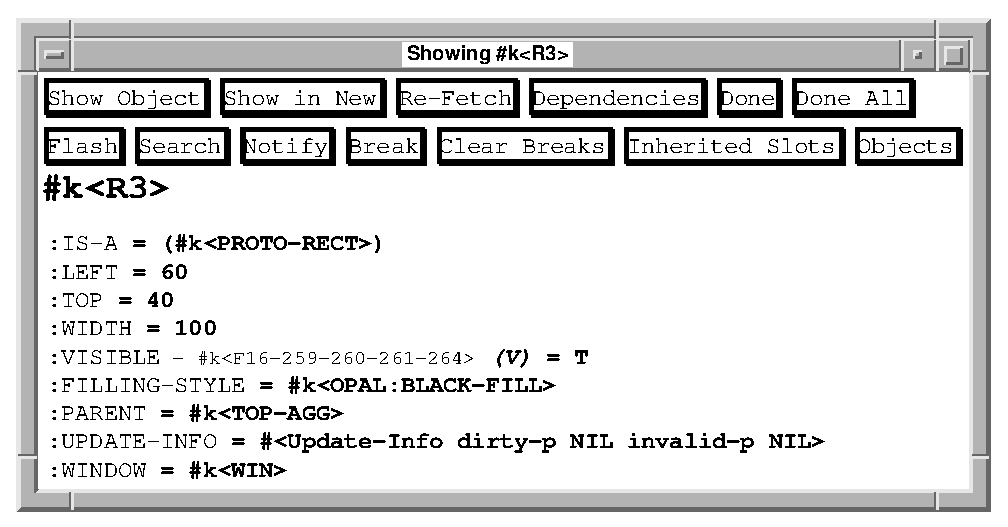
\epsfig{file=inspector.ps}
\end{center}
\caption{The Inspector displaying the slots and values of rectangle R3.}
\tag{inspector}
%\bar{}
\end{figure}

The local slots and values for R3 are shown in the Inspector window.
Inherited slots are not shown, like \pr{:height} or \pr{:line-style} (assuming
that you did not set these slots yourself, installing local values in R3).
If you have a color screen, some slots are red, indicating that these slots
are public `parameters' of the object (we discuss parameters more in
section \ref{parameters}).

It is very easy to change properties of an object with the Inspector.  For
example, to change the \pr{:width} of R3 using the inspector, click the mouse
on the value of the \pr{:width} slot (which is 100 in figure \ref{inspector}).
Use standard Emacs commands to change the value of the slot to something
significantly different, like 20.  When you hit RETURN, the change will appear
instantly in R3.

To add a new local value to R3 -- that is, to override an inherited value with
a new local value -- you have to add an extra line to the Inspector window.
In our example, R3 does not have a local value for \pr{:height}, since its
value is inherited from the prototype PROTO-RECT.  To override this value,
click the cursor at the end of a line, and type \pr{{\tt\char`\^}j} to add a new line
to the display.  Now you can type `\pr{:height = 100}' and hit RETURN to
install the new slot/value pair.  The change should be reflected instantly
in R3.

You can bring up other Inspector windows by positioning the mouse over another
object and hitting HELP again, or you can select text that is already displayed
in the Inspector and using the `\pr{Show Object}' or `\pr{Show in New}'
buttons.  For example, to examine the \pr{opal:black-fill} object that is the
value of R3's \pr{:filling-style} slot, either click-and-drag or double-click
on the \pr{\#k<OPAL:BLACK-FILL>} value and press the `\pr{Show in New}' button.
The object will be displayed in a new window.

When you are finished with the Inspector, you can click on the `\pr{Done}' or
`\pr{Done All}' buttons to make the Inspector windows disappear.

Significantly more detail about the Inspector is included in the Debugging
Manual, including how to explore the Prototype/Instance hierarchy of objects,
and how to use the Inspector for debugging more compilcated examples.


\section{Parameters}
\label{parameters}

Most objects in Garnet have a list of {\it parameters}, which are stored in the
\pr{:parameters} slot.  This is a list of all customizable properties of
the object.  For example, \pr{gv opal:rectangle :parameter} yields:
%\vspace{.5 line}

\begin{programexample}
(:LEFT :TOP :WIDTH :HEIGHT :LINE-STYLE :FILLING-STYLE :DRAW-FUNCTION :VISIBLE)
\end{programexample}

These can be considered the `public' slots of \pr{opal:rectangle}, which can
be given customized values when instances are created.  If values are not
supplied for these slots when instances are created, the default values will
be inherited from the prototype object.

There are other slots that change when instances of \pr{opal:rectangle} are
added to a window, such as the \pr{:window} and \pr{:parent} slots, but these
slots are not intended to be set manually.  Since they are `read-only' slots,
they are not included in the \pr{:parameters} list.

Several tools in Garnet rely heavily on the \pr{:parameters} slot.
As discussed in section \ref{inspector-sec}, the Inspector displays the
parameter slots in red, so that they are easily identified.  The
\pr{gg:prop-sheet} gadget which is used in Gilt and Lapidary looks at the
\pr{:parameters} slot to determine which slots should be displayed for the
user to customize.  These objects are discussed thoroughly in later sections
of this reference manual.

The typical Garnet user will not have to worry much about the \pr{:parameters}
slot.  All of the slots that are in the list are documented in this manual,
so it is really just another way to access the same information about
properties of objects.  For details on defining \pr{:parameters} slots for
your own objects, see the KR Manual.  Unless you are defining your own
list for a special object, the \pr{:parameters} slot should be considered
read-only.


\section{Destroying Objects}
\label{destroying}

Before moving on to the next section, destroy the window so that it
does not interfere with future examples in this tutorial.  Type the
following line.

\begin{programexample}
(opal:destroy WIN)
\end{programexample}
				
Destroying the window will also destroy all of the objects that were
added to its aggregate.  We can no longer manipulate R1, R2, and R3,
since they were destroyed by the previous call.  However, the
PROTO-RECT was never added to the top-level aggregate, and it was not
destroyed.  You could destroy this object now with a \pr{destroy}
call, but we will be using this object again in Section
\ref{destroying}.  So, leave the object residing in memory for now.

When an object is destroyed, its variable name becomes unbound and the
memory space that was allocated to the object is freed.  You can
\pr{destroy} any object, including windows.  If you destroy a window,
all objects inside of it are automatically destroyed.  Similarly, if
you destroy an aggregate, all objects in it are destroyed.  When you
destroy a graphical object (like a line or a circle), it is
automatically removed from any aggregate it might be in and erased
from the screen.

If a prototype object is destroyed (i.e., an object that has had
instances created from it), then all of the instances of that object
will be recursively destroyed.

Occasionally in the course of developing a program, you may (either
accidentally or intentionally) define a new object which happens to
have the same name as an old object.  When the new object is created,
its variable name is set to the new object, and the old object by the
same name is destroyed.  Also, all of the instances of the old object
are recursively destroyed.

For example, in Section \ref{prototypes} above, we created the object
PROTO-RECT, which still exists in memory.  If we now enter the
following new schema definition for an object by the same name, then
the old PROTO-RECT will be destroyed.

\begin{programexample}
(create-instance 'PROTO-RECT opal:rectangle)
\end{programexample}

When the new schema is entered, a warning is given that the old object
is being destroyed.  You can safely ignore this message, assuming that
you intended to override the definition of the old schema.


\section{Unnamed Objects}
\label{unnamed-objects}

Sometimes you will want to create objects that do not have a
particular name.  For example, you may want to write a function that
returns a rectangle, but it will be called repeatedly and should not destroy
previous instances with new ones.  In this case, you should return an
unnamed rectangle from the function which can be used just like the
named objects we have created earlier in this tutorial.

As an example, the following code creates an
unnamed object and internally generates a unique variable name for it.
Instead of supplying a quoted name to \pr{create-instance}, we give it
the value NIL.

\begin{programexample}
(create-instance NIL opal:rectangle
   (:left 10) (:top 10) (:width 75) (:height 50))
\end{programexample}

When you enter this schema definition, the \pr{create-instance} call
will return the generated internal name of the rectangle -- something like
\pr{RECTANGLE-123}.  This name has a unique number as a
suffix that prevents it from being confused with other rectangles in
Garnet.  You can now use the generated name to refer to the object.

\begin{programexample}
(gv RECTANGLE-123 :top)  {\it ; Replace this name with the name of your rectangle.}
\end{programexample}

Usually it is convenient to assign an unnamed object to a local
variable.  The following line creates a circle and assigns it to the
new variable MY-CIRCLE.

\begin{programexample}
(setf MY-CIRCLE (create-instance NIL opal:circle))
\end{programexample}

Now MY-CIRCLE will have the generated circle as its value.  If the
same line were entered again, the old circle would not be destroyed,
but the variable MY-CIRCLE would still point to a new one.  This can
be useful inside a function that uses a \pr{let} clause -- every time
the \pr{let} is executed, new objects are assigned to the local
variables, but the old objects still remain in memory and are not
destroyed. Section \ref{function} contains an example of how unnamed
objects might be used in a function.


\chapter{An Overview of the Objects}

\section{Lines, Rectangles, and Circles}

The Opal package provides different graphical shapes
including circles, rectangles, roundtangles, and lines.  There are
also several different kinds of text, and some special objects like
bitmaps and arrowheads.  Each graphical object has special slots that
determine its appearance, which are documented in the Opal manual.
(For example, the line uses the slots \pr{:x1}, \pr{:y1}, \pr{:x2},
and \pr{:y2}.)
See the section  `Specific Graphical Objects' in the Opal manual for
details of how each object works.  Examples of creating instances of
graphical objects appear throughout this tutorial.


\section{Aggregates}
\label{aggregates}

In order to put a large number of objects into a window, we might
create all of the objects and then add them, one at a time, to the
window.  However, this is usually not how
we organize the objects conceptually.  For example, if we were to
create a sophisticated interface with a scroll bar, several buttons,
and labels for the buttons, we would not want to add each rectangle in
the scroll bar and the buttons individually.  Instead, we would think
of creating the scroll bar from its composite rectangles, then
creating the buttons along with their labels, and then adding the
scroll bar assembly and the button assembly to the window.

Grouping objects together like this is the function of the \pr{aggregate}
object.  Any graphical object can be a component of an aggregate - lines,
circles, rectangles, and even other aggregates.  Usually all of the
components of an aggregate are related in some way, like they are all
parts of the same button.

Two other objects, the \pr{aggregadget} and the
\pr{aggrelist}, are also used to group objects, and usually appear more
often in Garnet programs.  \pr{Aggregadgets} and \pr{aggrelists} are
instances of \pr{aggregate}, and they have special features that make
them very useful in creating objects.  These objects will be discussed
further in Section \ref{aggregadgets}.

The top-level object in a window is always an aggregate.  This
aggregate contains all of the objects in that window.
Therefore, for an object to appear in a window it either has to be a
component of the top-level aggregate, or it has to be a component of
another aggregate which, at the top of its aggregate hierarchy, is a
component of the top-level aggregate.

When aggregates have other aggregates as components, an aggregate hierarchy
is formed.  This hierarchy describes the way that objects are grouped together.
Figure \ref{v-scroll-hierarchy} shows how the objects that comprise a
vertical scroll bar might be conceptually organized.

% \begin{group}
\begin{figure}
%\bar{}
\begin{center}
%\graphic{Postscript=`tutorial/v-scroll-hierarchy.ps',boundingbox=File,magnify=.75}
\epsfig{file=v-scroll-hierarchy.ps}
                 \end{center}
\caption{One possible hierarchy for the objects that make up a scroll bar.}
\tag{v-scroll-hierarchy}
%\bar{}
\end{figure}
% \end{group}

In the scroll bar hierarchy, all of the leaves correspond to shapes
that appear in the scroll bar.  The leaves are always Opal graphic
primitives, like rectangles and text.  The nodes \pr{top-trill-box} and
\pr{bottom-trill-box} are both aggregates, each with two components.
And, of course, the top-level \pr{scroll-bar} node is an aggregate.

This aggregate hierarchy should not be confused with the inheritance
hierarchy that was discussed earlier.  Components of an aggregate do
not inherit values from their parents.  Instead, relationships among
aggregates and components must be explicitly defined using
constraints, a concept which will be discussed shortly in this tutorial.

When an object is added to an aggregate, its \pr{:parent} slot is set
to point to that aggregate.  Therefore, in Figure \ref{v-scroll-hierarchy},
the \pr{:parent} of the \pr{bottom-trill-box} is the \pr{scroll-bar}
aggregate.  This \pr{:parent} slot is called a {\it pointer} slot because
its value is another Garnet object.  Pointer slots are discussed
further in section \ref{aggregadgets}.

The functions \pr{add-component}, \pr{remove-component},
and \pr{move-component} are used to manipulate the components of an
aggregate.  Descriptions of these and other functions for components
may be found in the `Aggregate Objects' section of the Opal manual.


\section{Aggregadgets, Aggrelists, and Aggregraphs}
\label{aggregadgets}

Aggregadgets and aggrelists are types of aggregates.  With these
objects, an aggregate and its components can basically be defined
simultaneously.  In aggregadgets, all the components are defined
with a list in the \pr{:parts} slot.  In an aggrelist, a single object
is defined to be an `item-prototype', and the aggrelist automatically
generates several instances of that object to make its components.
The aggregraph is a type of aggregadget, where all the components are
nodes and arcs that make up a graph.  Figures \ref{opalInheritance}
and \ref{v-scroll-hierarchy} were created using Garnet aggregraphs.
For several examples and a complete discussion of how to use
aggregraphs, see the Aggregadgets, Aggrelists, and Aggregraphs
Reference Manual.


\subsection{Aggregadgets}

When you create an aggregadget, you may list all of the objects that
you want as components of the aggregadget in the \pr{:parts} slot.
The list is specified using the standard Lisp backquote macro, and
there are usually many function calls and objects inside the list that
must be evaluated with a comma.  As an example of an aggregadget, we
will analyze the following schema definition, but it is not necessary
to type it in.  This code contains a few references that have not been
discussed in this tutorial yet, but it serves the purpose of giving us
a plain aggregadget to study.

\begin{programexample}
(create-instance 'AGG opal:aggregadget
   (:left 10) (:top 20)
   (:parts
    `((:my-circle ,opal:circle
                  (:left 60) (:top 70)
                  (:width 100) (:height 100)
                  (:line-style ,opal:dashed-line))
      (:my-rect ,opal:rectangle
                (:left ,(o-formula (gvl :parent :left)))
                (:top ,(o-formula (gvl :parent :top)))
                (:width 80) (:height 40)
                (:filling-style ,opal:black-fill)
                (:line-style NIL)))))
\end{programexample}

The \pr{:parts} slot in the AGG object contains
a list of lists, with each internal list being a definition of a component.
The components of AGG will be a circle and a rectangle, to which we
have given the arbitrary names \pr{:my-circle} and \pr{:my-rect}.
These names, which are preceded by a colon, will be the names of new
slots in the aggregadget.  That is, two {\it pointer} slots will be
created in AGG, named \pr{:my-circle} and \pr{:my-rect}, which will
have the circle and rectangle objects as their values.  We say these are
pointer slots because they point to other objects.

Other pointer slots which are automatically created are the
\pr{:parent} slots of both the circle and the rectangle.  Since these
objects are being added as components to the aggregadget, their
\pr{:parent} slots are set as with aggregates.  Thus, a two-way path
of communication is established between the aggregadget and each of
its components -- the \pr{:parent} slot points up, and the
\pr{:my-circle} slot points down.

Notice that the \pr{:parts} list is backquoted
(with a \pr{`} instead of a \pr{'}).  Using this backquote syntax, we can then
use commas to evaluate the names of objects inside the list.  The
references to be evaluated are the two graphical object prototypes (the
\pr{opal:circle} and the \pr{opal:rectangle}) and the graphical
qualities (\pr{opal:dashed-line} and \pr{opal:black-fill}).
Commas are also used to evaluate the \pr{o-formula} calls, which
establish constraints among objects (constraints are discussed
in Chapter \ref{constraints}).  If the commas were not present inside
the \pr{:parts} list, then the names of all the Garnet objects would not be
dereferenced, and they would be treated as mere atoms, not objects.
Similarly, the calls to \pr{o-formula} would appear as simple quoted
lists instead of function calls.

An important difference between aggregates and aggregadgets is that
when you create an instance of an aggregadget, the instance will
automatically have components that match those in the prototype.  That
is, if we created an instance of AGG, called AGG-INSTANCE, then
AGG-INSTANCE would automatically have a circle and rectangle component
just like AGG.  In contrast, when you create an instance of an
aggregate, the components are not automatically generated, and you
would have to create and add them to the instance manually.

Other examples of aggregadget definitions
can be found in sections \ref{aggregadget-ex} and \ref{big-example} in
this tutorial.

\subsection{Aggrelists}

An aggrelist allows you to create and easily arrange objects into a
nicely formatted graphical list.  The motivation for aggrelists comes
from the arrangement of groups of objects like button panels,
tic-marks, and menu choices, where all the components of an aggregate
are similar and should appear in a vertical or horizontal list.

In an aggrelist, a single item-prototype is defined, and then this
object is automatically copied several times to make the components of
the aggrelist.  The \pr{:left}, \pr{:top}, and other slots of the
components are automatically given values that will neatly lay out the
components in a list, so that the programmer does not have to do any
calculations for the positions of the objects.

As with aggregadgets, aggrelists
use the backquote syntax to define the item prototype.  There are many
customizable aspects of aggrelists, such as whether to orient the
components vertically or horizontally, the distance between each
object, etc.  Since there are so many customizable slots, please see
the Aggregadgets and Aggrelists Reference Manual for a discussion of
how to use aggrelists.  Section \ref{big-example} in this tutorial
includes an example of the definition of an aggrelist.


\section{Windows}

When we want to add an object to a window, what we really mean is that we
want to add the object to the window's top-level aggregate (or to an
aggregate at a lower level in that window's aggregate hierarchy).
Every window has one top-level aggregate, and all objects that appear
in the window are components in its aggregate hierarchy.

Any object must be added to a window in order for it to be shown on
the screen.  Additionally, a window must be updated before any changes
made to it (or the objects in it) will appear.  Windows are updated
when you explicitly issue a call to \pr{opal:update}, and they are
also continuously updated when interactors are running and changing
objects in the window (during the \pr{main-event-loop}, discussed in
Section \ref{interactors}).


\section{Gadgets}

The Garnet gadgets are a set of ready-made widgets that can be treated
as regular graphical objects.  They have slots that can be customized
with user-defined values, and are added to windows just like graphical
objects.  Generally, they are objects that are
commonly found in an interface including scroll bars, menus, buttons
and editable text fields.  In the Tour, you created instances of the
radio button panel and the vertical slider.  There are also more
sophisticated gadgets like scrolling windows, property sheets (to
allow quick editing of the slots of objects), and selection handles
(for moving and growing objects).

Most of the gadgets come in two versions -- one called the Garnet
Style, and one modeled after the OSF/Motif style.  Examples of how to
use the gadgets are found in demonstration programs at the end of each
of the gadget files, which can be executed by commands like
\pr{(garnet-gadgets:menu-go)}.  For detailed descriptions of all the
available gadgets, see the Gadgets Reference Manual.



\chapter{Constraints}
\label{constraints}

In the course of putting objects in a window, it is often desirable to
define relationships among the objects.  For example, you may want
the tops of several objects to be aligned, or you might want a set of
circles to have the same center, or you may want an object to change
color if it is selected.  Constraints are used in Garnet to define
these relationships among objects.

Although all the examples in this section use constraints on the
positions of objects, it should be clear that constraints can be
defined for filling styles, strings, or any other property of a Garnet
object.  Many examples of constraints can be found in other sections
of this tutorial.  Additionally, much of the KR Reference Manual is
devoted to the discussion of constraints among objects.  The sections
`Constraint Maintenance' and `Slot and Value Manipulation Functions'
should be of particular interest.


\section{Formulas}

A formula is an explicit definition of how to calculate the value for
a slot.  If we want to constrain the top of one object to be the same
as another, then we define a formula for the \pr{:top} slot of the dependent
object.  With constraints, the value of one slot always {\it depends} on
the value of one or more other slots, and we say the formula in that
slot has {\it dependencies} on the other slots.

An important point about constraints is that they are constantly
maintained by the system.  That is, they are evaluated once when they
are first created, and then they are continually {\it re-evaluated} when
any of their dependencies change.  Thus, if several objects depend on
the top of a certain rectangle, then all the objects will change
position whenever the rectangle is moved.

\begin{figure}
%\bar{}
\begin{center}
%\graphic{Postscript=`tutorial/align-top.ps',boundingbox=File,magnify=.75}
\epsfig{file=align-top.ps}
\end{center}
\caption{Three objects that are all aligned with the same top.  The
top of the gray rectangle is constrained to the white rectangle, and
the top of the black circle is constrained to the top of the gray rectangle.}
\tag{align-top}
%\bar{}
\end{figure}

As our first example of defining constraints among objects, we will
make the window in Figure \ref{align-top}.  Let's begin by creating
the white rectangle at an absolute position, and then create the other objects
relative to it.  Create the window and the first box with the
following code.

\begin{programexample}
(create-instance 'CONSTRAINTS-WIN inter:interactor-window      {\it ; Create the window}
   (:left 750)(:top 80)(:width 260)(:height 100))
(create-instance 'TOP-AGG opal:aggregate)                      {\it ; Create an aggregate}
(s-value CONSTRAINTS-WIN :aggregate TOP-AGG)                   {\it ; Assign the aggregate to the window}
(opal:update CONSTRAINTS-WIN)                                  {\it ; Make the window appear}

(create-instance 'WHITE-RECT opal:rectangle                    {\it ; Create a rectangle}
   (:left 20) (:top 30)
   (:width 60) (:height 40)
   (:filling-style opal:white-fill))
		
(opal:add-components TOP-AGG WHITE-RECT)                       {\it ; Add the rectangle to the window}
(opal:update CONSTRAINTS-WIN)                                  {\it ; Make changes in the window appear}
\end{programexample}

We are now ready to create the other objects that are aligned with
WHITE-RECT.  We could simply create another rectangle and a circle that
each have their top at 30, but this would lead to extra work if we ever
wanted to change the top of all the objects, since each object's
\pr{:top} slot would have to be changed individually.  If we instead
define a relationship that depends on the top of WHITE-RECT, then
whenever the top of WHITE-RECT changes, the top of the other objects
will automatically change, too.  Define the schema for the gray
rectangle as follows.

\begin{programexample}
(create-instance 'GRAY-RECT opal:rectangle
   (:left 110)
   (:top (o-formula (gv WHITE-RECT :top)))  {\it ; Constrain the top of this rectangle to the top of WHITE-RECT}
   (:width 60) (:height 40)
   (:filling-style opal:gray-fill))

(opal:add-components TOP-AGG GRAY-RECT)
(opal:update CONSTRAINTS-WIN)
\end{programexample}

You can see that without specifying an absolute position for the top
of the gray rectangle, we have constrained it to always have the same
top as the white rectangle.  The formula in the \pr{:top} slot of
the gray rectangle was defined using the functions \pr{o-formula} and
\pr{gv}.  The \pr{o-formula} function is used to declare that an
expression is a constraint.  When \pr{gv} is used inside a formula,
it causes a dependency to be established on the referenced slot, so that
the formula will be reevaluated when the value in the referenced slot
changes.  \footnote{There is another function called \pr{g-value}
that is similar
to \pr{gv}, except that it never causes dependencies to be established.
Older versions of Garnet required that \pr{gv} only be used inside
formulas, and \pr{g-value} to be used ouside.  The \pr{gv} function has
since been enhanced so that it can be used everywhere.  It would be
unusual to ever need to use \pr{g-value}.}

To see if our constraint is working, try changing the
top of the white rectangle with the following instructions and notice
how the gray rectangle moves with it.  Try setting the top to other
values, if you wish.

\begin{programexample}
(s-value WHITE-RECT :top 50)
(opal:update CONSTRAINTS-WIN)
\end{programexample}

The important thing to notice is that the value of the \pr{:top} slot
of GRAY-RECT changes as the top of the WHITE-RECT changes.  This shows
that the formula in GRAY-RECT is being re-evaluated whenever its
depended values change.

Now we are ready to add the black circle to the window.  We have a
choice of whether to constrain the top of the circle to the white
rectangle or the gray rectangle.  Since we are going to be examining
these objects closely in the next few paragraphs, let's constrain the
circle to the gray rectangle, resulting in an indirect relationship with
the white one.  Define the black circle with the following code.

\begin{programexample}
(create-instance 'BLACK-CIRCLE opal:circle
   (:left 200)
   (:top (o-formula (gv GRAY-RECT :top)))
   (:width 40) (:height 40)
   (:filling-style opal:black-fill))

(opal:add-components TOP-AGG BLACK-CIRCLE)
(opal:update CONSTRAINTS-WIN)
\end{programexample}

At this point, you may want to set the \pr{:top} of the white
rectangle again just to see if the black circle follows along with
the gray rectangle.


\section{Cached Values}

An interesting question might have occurred to
you -- what happens if you set the \pr{:top} of the gray rectangle now?
Setting the value of a slot which already has a formula in it does {\it not}
destroy the existing constraint.  However, it does override the
current {\it cached} value of the formula.  Try setting the \pr{:top} of
the gray rectangle now.

\begin{programexample}
(s-value WHITE-RECT :top 30)  {\it ; Return everything to its original position}
(opal:update CONSTRAINTS-WIN)

(s-value GRAY-RECT :top 40)
(opal:update CONSTRAINTS-WIN)
\end{programexample}

The position of WHITE-RECT will remain unchanged, since it was defined with
an absolute position.  However, the new value that we gave for the top
of the gray rectangle has repositioned GRAY-RECT and BLACK-CIRCLE.
Previously, the formula in the \pr{:top} slot of GRAY-RECT had
correctly computed its own top, getting the value from the \pr{:top}
slot of WHITE-RECT.  Now, however, we replaced that cached value
with our absolute value of 40.

To show that the formula is still alive and well in the \pr{:top} slot
of GRAY-RECT, try setting the \pr{:top} slot of WHITE-RECT again.

\begin{programexample}
(s-value WHITE-RECT :top 10)
(opal:update CONSTRAINTS-WIN)
\end{programexample}

Since the top of GRAY-RECT depends on WHITE-RECT, its formula will be
recomputed whenever the top of WHITE-RECT changes.  There is now a new
cached value for the \pr{:top} of GRAY-RECT, a result of re-evaluating
the formula.


\section{Formulas and s-value}

It is important to distinguish the behavior of \pr{s-value} when it is
used on a slot with a formula in it, versus using it on a slot with an
absolute value in it (like the number 5).  Setting the value of a slot that
{\it already} has a formula in it will not destroy the old formula.
Instead, only the cached value of the formula is changed, and the
formula will be re-evaluated if any of its dependencies change.

On the other hand, \pr{s-value} will replace one absolute value with
another absolute value, and the old value will never appear again.
That is, if an object was created with some particular absolute value for a
slot, and we changed that slot with \pr{s-value}, then the new value
will be permanent until the slot is explicitly set again with \pr{s-value}.

The one exception to the above rules is when the new value is a
formula itself.  Using \pr{s-value} to set a new formula will always
obliterate what was previously in the slot, whether it was an absolute
value or a formula.


\section{Using the :obj-over Slot}
\label{obj-over-slot}

When designing an interface, you may want a box to be drawn
around an object to show that it is selected.  In the usual case, you
will want to define only one box that will be drawn around different
objects, and it would be nice if the box changed size when it was over
objects of different size.  The traditional Garnet approach to this
problem is to use constraints in the dimension slots of the selection
box that depend on the dimensions of the object it is over.

\begin{figure}
%\bar{}
\begin{center}
%\graphic{Postscript=`tutorial/obj-over.ps',boundingbox=File, magnify=.75}
\epsfig{file=obj-over.ps}
\end{center}
\caption{A selection box drawn around an object.}
\tag{obj-over}
%\bar{}
\end{figure}

In the traditional approach, we use the slot \pr{:obj-over} in the
selection box to specify which object the selection box should be
drawn around.  The \pr{:obj-over} slot is a pointer slot, since it
contains an object as its value (pointer slots were discussed in
section \ref{aggregadgets}).  Then, we define formulas for the
dimensions of the selection box which depend on the \pr{:obj-over}
slot.  The formulas in the following schema definition should be clear.

\begin{programexample}
(create-instance 'SEL-BOX opal:rectangle
   (:obj-over GRAY-RECT)  {\it ; A pointer slot}
   (:left (o-formula (- (gvl :obj-over :left) 10)))
   (:top (o-formula (- (gvl :obj-over :top) 10)))
   (:width (o-formula (+ 20 (gvl :obj-over :width))))
   (:height (o-formula (+ 20 (gvl :obj-over :height))))
   (:line-style opal:line-4))  {\it ; A line with a thickness of 4 pixels}
		
(opal:add-components TOP-AGG SEL-BOX)
(opal:update CONSTRAINTS-WIN)
\end{programexample}

Now if you set the \pr{:obj-over} slot of the selection box to be a
different object, the position and dimensions of SEL-BOX will change
according to the object.

\begin{programexample}
(s-value SEL-BOX :obj-over BLACK-CIRCLE)
(opal:update CONSTRAINTS-WIN)
\end{programexample}

You may have noticed that we performed computations in the formulas
above, instead of just using values directly as in the GRAY-RECT and
BLACK-CIRCLE objects.  In fact, formulas can contain any lisp
expression.  Also, the formulas above use the function \pr{gvl}
instead of \pr{gv}, which was used earlier.  We use \pr{gvl} here
because we are referencing a slot, \pr{:obj-over}, in the same schema
as the formula.  Previously, we used \pr{gv} to look at a slot in a
different object.

Another point of interest in these formulas is the use of indirect
references.  In the \pr{:left} formula above, the pointer slot \pr{:obj-over}
is referenced, and then its \pr{:left} slot is referenced, in turn.
It is important to distinguish between this case and the case where
a value is stored in the same object as the formula, as in the
following example.

Suppose we want the selection box to become invisible if no object is
currently selected.  Using \pr{s-value}, we can set the \pr{:visible}
slot of SEL-BOX to have a formula which will cause the box to
disappear when its current selection is NIL.  (We could have also
defined this formula in the \pr{create-instance} call.)

\begin{programexample}
(s-value SEL-BOX :visible (o-formula (gvl :obj-over)))
\end{programexample}

Clearly, if \pr{:obj-over} is set to NIL, then the value in the
\pr{:visible} slot will also become NIL, and the box will become
invisible.  When \pr{:obj-over} is again set to be some object, then
the \pr{:visible} slot will have a non-NIL value, and the box will
appear in the appropriate position.  Previously, if we had set
\pr{:obj-over} to NIL, then updating the window would have caused an
error when the formulas tried to access the \pr{:left}, \pr{:top},
\pr{:width}, and \pr{:height} of the non-existent selected object.

We are finished with the objects from this section, but the next
section will continue to use the same window.  So, to remove the old
objects from the window, use the function \pr{remove-components}.

\begin{programexample}
(opal:remove-components TOP-AGG WHITE-RECT GRAY-RECT BLACK-CIRCLE SEL-BOX)
(opal:update CONSTRAINTS-WIN)
\end{programexample}


\section{Constraints in Aggregadgets}
\label{aggregadget-ex}

As mentioned in section \ref{aggregates}, the \pr{:parent} slot of a
component is automatically set to its parent aggregate when it is
attached.  Since aggregadgets are instances of aggregates, all of the
components defined in an aggregadget have their \pr{:parent} slot set
in this way.  In this section, we will examine how this slot can be
used to communicate between components of an aggregadget.

% \vspace{1 line}
%\begin{group}
The aggregadget we will use in this example will make the picture of
concentric circles in Figure \ref{concentric-circles}.  Suppose that
we want to be able to change the size and position of the circles
easily, and that this should be done by setting as few slots as
possible.
% \end{group}
% \vspace{.5 line}

\begin{figure}
%\bar{}
\begin{center}
% graphic{Postscript=`tutorial/con-circles.ps',boundingbox=File}
\epsfig{file=con-circles.ps}\end{center}
\caption{An aggregadget with three circles as components.}
\tag{concentric-circles}
%\bar{}
\end{figure}

From the picture, we see that the dimensions of the black circle are
the same as the dimensions of the entire group of objects.  That is,
if a bounding box were drawn around the black circle, all the other
objects would be inside the bounding box, too.
Therefore, it will be helpful to put slots for the size and position
of this circle in the top-level aggregadget, and have all the circles
reference these top-level values through formulas.

To start, let's create an aggregadget with only one component -- the
black circle -- and then redefine the aggregadget with the other
components later.  The following code creates this one-component
aggregate.

\begin{programexample}
(create-instance 'CON-CIRCLES opal:aggregadget
   (:left 20) (:top 20)
   (:width 100)
   (:height (o-formula (gvl :width)))
   (:parts
    `((:black-circle ,opal:circle
                     (:left ,(o-formula (gvl :parent :left)))
                     (:top ,(o-formula (gvl :parent :top)))
                     (:width ,(o-formula (gvl :parent :width)))
                     (:height ,(o-formula (gvl :width)))
                     (:filling-style ,opal:black-fill)))))

(opal:add-component TOP-AGG CON-CIRCLES)
(opal:update CONSTRAINTS-WIN)
\end{programexample}

All those commas are needed because we want the Opal objects and the
calls to \pr{o-formula} to be evaluated inside the backquoted list.
If the commas were not present, then those forms would become inert
atoms and lists instead of objects and function calls.

The black circle in the aggregadget gets its position and
dimensions from the top-level slots in CON-CIRCLES.  The communication
link used here is the \pr{:parent} slot, which points from the
component to the aggregadget.  The function
\pr{gvl} is used in the formulas for the black circle because the
\pr{:parent} slot is in the same object as the formulas.  Notice that
the black circle does {\it not} `inherit' any values from its parent.
Creating components in an aggregadget sets up an {\it aggregate}
hierarchy, where values travel back-and-forth over constraints,
not inheritance links.  If you want a component to depend on values in
its parent, you have to define constraints.

The other components of CON-CIRCLES will be defined analogously, but with
a little more computation in the formulas to get them to line up properly.
Before typing in the new definition of CON-CIRCLES, remove the old
aggregadget from the window with the following instruction.

\begin{programexample}
(opal:remove-components TOP-AGG CON-CIRCLES)
(opal:update CONSTRAINTS-WIN)
\end{programexample}

And now we are ready to redefine CON-CIRCLES again, this time with an
extra top-level slot to reduce redundant calculations, and of course
with the other two circles.

\begin{programexample}
(create-instance 'CON-CIRCLES opal:aggregadget
   (:left 20) (:top 20)
   (:width 100)
   (:height (o-formula (gvl :width)))
   (:radius/3 (o-formula (round (gvl :width) 6)))
   (:parts
    `((:black-circle ,opal:circle
                     (:left ,(o-formula (gvl :parent :left)))
                     (:top ,(o-formula (gvl :parent :top)))
                     (:width ,(o-formula (gvl :parent :width)))
                     (:height ,(o-formula (gvl :width)))
                     (:filling-style ,opal:black-fill))
      (:gray-circle ,opal:circle
                    (:left ,(o-formula (+ (gvl :parent :left)
					  (gvl :parent :radius/3))))
                    (:top ,(o-formula (+ (gvl :parent :top)
					 (gvl :parent :radius/3))))
                    (:width ,(o-formula (- (gvl :parent :width)
					   (* 2 (gvl :parent :radius/3)))))
                    (:height ,(o-formula (gvl :width)))
                    (:filling-style ,opal:gray-fill))
      (:white-circle ,opal:circle
                     (:left ,(o-formula (+ (gvl :parent :gray-circle :left)
					   (gvl :parent :radius/3))))
                     (:top ,(o-formula (+ (gvl :parent :gray-circle :top)
					  (gvl :parent :radius/3))))
                     (:width ,(o-formula (- (gvl :parent :gray-circle :width)
					    (* 2 (gvl :parent :radius/3)))))
                     (:height ,(o-formula (gvl :width)))
                     (:filling-style ,opal:white-fill)))))

(opal:add-components TOP-AGG CON-CIRCLES)
(opal:update CONSTRAINTS-WIN)
\end{programexample}

The gray circle gets its size and position from the top-level slots
just like the black circle, only it is one-third the size.  The white circle
is the most interesting case, where it gets its position and
dimensions from the gray circle.  Not only does the white circle
communicate with the aggregadget through the \pr{:parent} slot, but it
also uses the slot \pr{:gray-circle} which was automatically created
in the aggregadget (see section \ref{aggregadgets}).  Thus, the
formulas in the white circle trace up the aggregate hierarchy to the
parent aggregadget, and then back down into another component.

To examine these pointer slots more closely, try executing the
following line.

\begin{programexample}
(gv CON-CIRCLES :white-circle)
\end{programexample}

The value returned by this \pr{gv} call is the internally
generated name of the white circle.  This name was generated with a
unique suffix number so that it will not be confused with some other
white circle in Garnet (see Section \ref{unnamed-objects}).  You can
also look at slots of the components directly, by adding slot names to
the end of the \pr{gv} call, like

\begin{programexample}
(gv CON-CIRCLES :white-circle :top)
\end{programexample}

or even

\begin{programexample}
(gv CON-CIRCLES :white-circle :parent)
\end{programexample}

This is the end of the section regarding constraints.  Destroy the window
we have been using to keep it from interfering with future examples in
the tutorial.

\begin{programexample}
(opal:destroy CONSTRAINTS-WIN)
\end{programexample}



\chapter{Interactors}
\label{interactors}

Interactors are used to communicate with the mouse and keyboard.
Sometimes you may just want a function to be executed when the mouse
is clicked, but often you will want changes to occur in the graphics
depending on the actions of the mouse.  Examples include moving
objects around with the mouse, editing text with the mouse and
keyboard, and selecting an object from a given set.

The fundamental way that the interactors communicate with graphical
objects is that they set slots in the objects in response to mouse
movements and keyboard key strokes.  That is, they generate side
effects in the objects that they operate on.  For example, some interactors
set the \pr{:selected} and \pr{:interim-selected} slots to indicate which
object is currently being operated on.  When objects are defined with
formulas that depend on these special slots, the appearance of the
objects (i.e., the graphics of the interface) can change in response
to the mouse.

It is important to note that all of the gadgets come with their
interactors already defined.  Therefore, you do not need to create
interactors that change the gadgets.

In this section we will see some examples of how to change graphics in
conjunction with interactors.  Section \ref{trace-inter} describes how
to use an important debugging function for interactors called
\pr{trace-inter}.   Although this tutorial only gives examples of
using the \pr{button-interactor} and \pr{move-@{\tt\char`\|}grow-@{\tt\char`\|}interactor}, the
Interactors Manual discusses and provides examples for all six types
of Garnet interactors.


\section{Kinds of Interactors}

The design of the interactors is based on the observation that there
are only a few kinds of behaviors that are typically used in graphical
user interfaces.  Currently, Garnet supports seven types of interactive
behavior, which allows a wide variety of user actions in an interface.
Below is a list of the available interactors, which are described in
detail in the Interactors Manual.

\begin{description}
\item[] \pr{Menu-Interactor} - For selecting one or more choices from a set of
items.  Useful in menus, etc., where the mouse may be held down and
dragged while moving over the items to be selected.

\item[] \pr{Button-Interactor} - For selecting one or more choices from a set
of items.  Useful in single buttons and panels of buttons where the
mouse can only select one item per mouse click.

\item[] \pr{Move-Grow-Interactor} - For moving and changing the size of an
object.  Useful in scroll bars and graphics editors.

\item[] \pr{Two-Point-Interactor} - For obtaining one or two points in a
window from the user.  Useful in specifying the size and position of a
new object to be created.

\item[] \pr{Angle-Interactor} - For getting the angle that the mouse moves
around a point.  Useful in circular gauges or for `stirring motions'.

\item[] \pr{Text-Interactor} - For editing strings.  Most useful for small
strings, since Garnet does not support complicated word-processing
applications.

\item[] \pr{Gesture-Interactor} - For recognizing gestures drawn by the user
(e.g., the user draws a rough shape that Garnet recognizes as a square).

\item[] \pr{Animator-Interactor} - For executing a function at regular intervals,
allowing rapid updating of graphics.
\end{description}

There are also several interactors that work with the \pr{multifont-text}
object.  This object and its associated interactors are discussed in
the Opal manual.


\section{The Button Interactor}

In this example, we will perform an elementary operation with an
interactor.  We will create a window with a white rectangle inside,
and then create an interactor that will make it change colors when
the mouse is clicked inside of it.  First, create the window with the
white rectangle.

\begin{programexample}
(create-instance 'INTER-WIN inter:interactor-window
   (:left 750)(:top 80)(:width 250)(:height 250))
(create-instance 'TOP-AGG opal:aggregate)
(s-value INTER-WIN :aggregate TOP-AGG)
(opal:update INTER-WIN)

(create-instance 'CHANGING-RECT opal:rectangle
   (:left 20) (:top 30)
   (:width 60) (:height 40)
   (:filling-style (o-formula (if (gvl :selected)
				  opal:black-fill
				  opal:white-fill)))
   (:selected NIL))  {\it ; Set by the interactor}

(opal:add-components TOP-AGG CHANGING-RECT)
(opal:update INTER-WIN)
\end{programexample}

From the definition of the \pr{:filling-style} formula, you can see
that if the \pr{:selected} slot in CHANGING-RECT were to be set to be
non-NIL, then its color would turn to black.  Conveniently, setting the
\pr{:selected} slot is one of the side effects of the
\pr{button-interactor}. The following code defines an interactor which
will set the \pr{:selected} slot of CHANGING-RECT, which will cause it
to change colors.

\begin{programexample}
(create-instance 'COLOR-INTER inter:button-interactor
   (:window INTER-WIN)
   (:start-where (list :in CHANGING-RECT))
   (:start-event :leftdown))

{\it ; Unless using CMU, Allegro, Lucid, LispWorks, or MCL}
(inter:main-event-loop)
{\it ; Hit F1 while the mouse is in the Garnet window to exit}
\end{programexample}

The \pr{main-event-loop} function causes Garnet to start paying
attention to events (like clicking the mouse) that trigger the interactors.
(A background process in CMU, Allegro, Lucid, LispWorks, and MCL always
pays attention to events.)
Now you can click on the rectangle
repeatedly and it will change from white to black, and back again.
From this observation, and knowing how we defined the
\pr{:filling-style} of CHANGING-RECT, you can conclude that the
\pr{button-interactor} is setting (and clearing) the \pr{:selected}
slot of the object.  This is one of the functions of the
\pr{button-interactor}.
When you are ready to resume typing in the Lisp process, you have to
hit the F1 key while the mouse is in the Garnet window to get a new
prompt.  (You may execute the \pr{main-event-loop} call again at any
Lisp prompt.)

\begin{figure}
%\bar{}
\begin{center}
% graphic{Postscript=`tutorial/inter-white.ps',boundingbox=File}
\epsfig{file=inter-white.ps}  % graphic{Postscript=`tutorial/inter-black.ps',boundingbox=File}
\epsfig{file=inter-black.ps}\end{center}
\caption{The rectangle CHANGING-RECT when its \pr{:selected} slot is NIL
(the default), and when it is set to T by the interactor (when the
mouse is clicked over it).}
%\bar{}
\end{figure}


\section{A Feedback Object with the Button Interactor}
\label{button-feed}

The method we used in the previous section with the
\pr{button-interactor} involved setting the \pr{:selected} slot of the
selected object.  There is another way to use the button interactor
which involves using feedback objects.  A {\it feedback object} is some
object that indicates the currently selected object.  For example, it is
often desirable that the actual selected object not move or change
color, but rather that a separate object follow the mouse or appear
over the selection.

In an earlier example in section \ref{obj-over-slot}, we defined a
selection box which works just like a feedback object.  When the
\pr{:obj-over} slot of the selection box was set to the name of the
selected object, then the box appeared around the selected object.  In this
example, we will redefine the objects from that section and create an
interactor to work on them.

The following code is analogous to what was presented in section
\ref{obj-over-slot}, but here the three selectable objects are defined as
components in an aggregadget.  Type in the following aggregadget and
feedback object, and add them to the current window.  Notice that
because of the \pr{:visible} formula in FEEDBACK-RECT, that rectangle
will be invisible when the window is first updated.

\begin{programexample}
(create-instance 'AGG opal:aggregadget
   (:top 100)
   (:parts
    `((:white-rect ,opal:rectangle
                   (:left 20)
                   (:top ,(o-formula (gvl :parent :top)))
                   (:width 60)
                   (:height 40)
                   (:filling-style ,opal:white-fill))
      (:gray-rect ,opal:rectangle
                  (:left 110)
                  (:top ,(o-formula (gvl :parent :top)))
                  (:width 60)
                  (:height 40)
                  (:filling-style ,opal:gray-fill))
      (:black-circle ,opal:circle
                     (:left 200)
                     (:top ,(o-formula (gvl :parent :top)))
                     (:width 40)
                     (:height 40)
                     (:filling-style ,opal:black-fill)))))

(create-instance 'FEEDBACK-RECT opal:rectangle
   (:obj-over NIL)  {\it ; A pointer slot to be set by the interactor}
   (:visible (o-formula (gvl :obj-over)))
   (:left (o-formula (- (gvl :obj-over :left) 10)))
   (:top (o-formula (- (gvl :obj-over :top) 10)))
   (:width (o-formula (+ 20 (gvl :obj-over :width))))
   (:height (o-formula (+ 20 (gvl :obj-over :height))))
   (:line-style opal:line-4))

(opal:add-components TOP-AGG AGG FEEDBACK-RECT)
(opal:update INTER-WIN)
\end{programexample}

Notice that the \pr{:obj-over} slot of FEEDBACK-RECT is a pointer
slot, as usual.  When \pr{:obj-over} is set with the name of an
object, the FEEDBACK-RECT will appear over the object because of the
way we defined its position and dimension formulas.  In this example,
we will not set \pr{:obj-over} by hand, as we did previously.
Instead, we will create a \pr{button-interactor} to set the slot for us.

The following code defines an interactor which uses the FEEDBACK-RECT
to indicate which object is selected.  Since all of the selectable
objects are in the same aggregate, we can tell the interactor to start
whenever the mouse is clicked over any component of AGG.

\begin{programexample}
(create-instance 'SELECTOR inter:button-interactor
   (:window INTER-WIN)
   (:start-where (o-formula (list :element-of AGG)))  {\it ; Work on the components of AGG}
   (:final-feedback-obj FEEDBACK-RECT)
   (:how-set :toggle))

{\it ; Unless using CMU, Allegro, Lucid, LispWorks, or MCL}
(inter:main-event-loop)
{\it ; Hit F1 while the mouse is in the Garnet window to exit}
\end{programexample}

Now when you click on the objects, the feedback object will appear
over the selected object.  The reason is that the
\pr{button-interactor} sets the \pr{:obj-over} slot of the feedback
object.  Since the interactor is a toggling
interactor (according to its \pr{:how-set} slot), the \pr{:obj-over}
slot will be reset to NIL when the selected object is clicked on again.

If you entered the \pr{main-event-loop}, remember to hit the F1 key
before typing in the next example.


\section{The Move-Grow Interactor}

From the previous example, you can see that it is easy to change the
graphics in the window using the mouse.  We are now going to define several
more objects in the window and create an interactor to move them.

The side effect of the \pr{move-grow-interactor} is that it sets the
\pr{:box} slot of the selected object (as well as the feedback object,
if any) to be a list of four values -- the left, top, width, and
height of the object.  When formulas are defined in the \pr{:left},
\pr{:top}, \pr{:width}, and \pr{:height} slots which depend on
the \pr{:box} slot, then the position and dimensions of the
object will change whenever the \pr{:box} slot changes.

The idea goes like this:  Suppose the current value of the \pr{:box}
slot in a rectangle is '(0 0 40 40).  Since the \pr{:left} and
\pr{:top} slots are constrainted to the \pr{:box} slot, the rectangle
appears at the position (0,0).  To move the object, the user clicks
and drags on the rectangle until it is at position (50,50).  When the
user lets go, then the interactor automatically sets the \pr{:box}
slot to '(50 50 40 40).  Since the \pr{:box} slot has changed, the
formulas in the \pr{:left} and \pr{:top} slot are re-evaluated, and
the rectangle appears at the new position.

The following code creates a prototype circle and several instances of
it.  With a little study, it should be clear how the position and dimension
formulas work with respect to the \pr{:box} slot.  All of the circles
are then added to an aggregate, and this aggregate is added as a
component to the top-level aggregate.

\begin{programexample}
(create-instance 'MOVING-CIRCLE opal:circle
   (:box '(0 0 40 40))  {\it ; This slot will be set by the interactor}
   (:left (o-formula (first (gvl :box))))     {\it ; Get the first value in the list}
   (:top (o-formula (second (gvl :box))))
   (:width (o-formula (third (gvl :box))))
   (:height (o-formula (fourth (gvl :box)))))

(create-instance 'M1 MOVING-CIRCLE
   (:box '(120 30 40 40)))

(create-instance 'M2 MOVING-CIRCLE
   (:box '(30 100 60 60)))

(create-instance 'M3 MOVING-CIRCLE
   (:box '(120 100 80 80)))

(create-instance 'CIRCLE-AGG opal:aggregate)

(opal:add-components CIRCLE-AGG M1 M2 M3)		

(opal:add-components TOP-AGG CIRCLE-AGG)
(opal:update INTER-WIN)
\end{programexample}

If you want to try setting the \pr{:box} slot of any of these objects,
you will see how the position and dimension of each circle depend on
it.  Be sure you set the \pr{:box} slot to be a list of four positive
numbers, or an error will occur!

Now let's create an instance of the \pr{move-grow-interactor}, which
will cause the moving circles to change position.  The following
interactor works on all the components of the aggregate CIRCLE-AGG.
Remember to execute the \pr{inter:main-event-loop} call to start the
interactors working.

\begin{programexample}
(create-instance 'MG-INTER inter:move-grow-interactor
   (:window INTER-WIN)
   (:start-where (list :element-of CIRCLE-AGG)))    {\it ; Work on the components of CIRCLE-AGG}

{\it ; Unless using CMU, Allegro, Lucid, LispWorks, or MCL}
(inter:main-event-loop)
{\it ; Hit F1 while the mouse is in the Garnet window to exit}
\end{programexample}

Now if you press and drag in any of the circles, they will follow the
mouse.  This is because the interactor sets the \pr{:box} slot of the
object that it is pressed over, and the \pr{:left} and \pr{:top} slots
of the objects depend on the \pr{:box} slot.

It is worth noting once again that the \pr{move-grow-interactor} does
{\it not} set the \pr{:left}, \pr{:top}, etc. slots of the selected
object.  It instead sets the {\it \pr{:box}} slot of the selected
object, and the user is required to define formulas that depend on the
\pr{:box} slot.


\section{A Feedback Object with the Move-Grow Interactor}

Now let's add a feedback object to the window that will work with the
moving circles.  In this case, the feedback object will appear
whenever we click on and try to drag a circle.  The mouse will
actually drag the feedback object, and then the real circle will jump
to the final position when the mouse is released.

Our feedback object will be a circle with a dashed line.  The
DASHED-CIRCLE object defined below will have two slots set by the
interactor.  The \pr{:box} slot will be set while the mouse is held
down and dragged, and the \pr{:obj-over} slot will be set to point to the
circle being dragged.  Given our MOVING-CIRCLE prototype, the feedback
object is easy to define.

\begin{programexample}
(create-instance 'DASHED-CIRCLE MOVING-CIRCLE
   {\it ; Inherit all the :left, :top, etc. formulas that depend on the :box slot.}
   (:obj-over NIL)  {\it ; Set by the interactor}
   (:visible (o-formula (gvl :obj-over)))
   (:line-style opal:dashed-line))

(opal:add-components TOP-AGG DASHED-CIRCLE)
\end{programexample}

The \pr{:visible} slot is set with a formula because we only want the
feedback object to be visible when it is being used with the
interactor.  Now, we will redefine the move-grow interactor to use
DASHED-CIRCLE as a feedback object.  (Redefining the MG-INTER will
destroy the old instance, so don't worry if a warning appears.)

\begin{programexample}
(create-instance 'MG-INTER inter:move-grow-interactor
   (:window INTER-WIN)
   (:start-where (list :element-of CIRCLE-AGG))
   (:feedback-obj DASHED-CIRCLE))
\end{programexample}

Now when you move the circles with the mouse, the feedback object will
follow the mouse, instead of the real circle following it directly.

Since we have finished this section on interactors, destroy the window
so that it does not interfere with the next example.  Type the
following line.

\begin{programexample}
(opal:destroy INTER-WIN)
\end{programexample}


\chapter{Programming}

\section{Creating a Panel of Text Buttons}
\label{big-example}

In this section, we will go through a comprehensive example that pulls
together all the concepts that have been discussed in this tutorial.
The final objective will be the panel of text buttons in Figure
\ref{textButtons}.  We will use an aggregadget to assemble a group
of objects into a single button, then use an aggrelist to make
multiple copies of the text button and organize them into a list for
the panel, and finally create a button interactor to manage the panel.


\subsection{The Limitations of Aggregates}

Before starting the aggregadget for this example, let's take a look at the use
of an aggregate.  This will help to demonstrate the usefulness of
aggregadgets.  First, create a window with a top-level aggregate and
update it:

\begin{programexample}
(create-instance 'BUTTON-WIN inter:interactor-window
   (:left 800)(:top 10)(:width 200)(:height 400))
(create-instance 'TOP-AGG opal:aggregate)
(s-value BUTTON-WIN :aggregate TOP-AGG)
(opal:update BUTTON-WIN)
\end{programexample}

The TOP-AGG aggregate is the top-level aggregate for the window.  If
we want any object to appear in the window, it will have to be added
to TOP-AGG, or added to an aggregate further below in TOP-AGG's
aggregate hierarchy.  We will keep TOP-AGG as the top-level aggregate
throughout this example, but we will be changing its components continually.

Now we can begin adding objects to TOP-AGG (throughout this discussion
you should periodically check Figure \ref{textButtons} to see why we
are creating particular objects).  Let's start by assembling a button.
We will first create a couple of rectangles that have a fixed position
so that we get the window in Figure \ref{twoRects}.  Since we
want the rectangles to have the same dimensions, we can make a
prototype object and then create two instances with appropriate
position values.

\begin{programexample}
(create-instance 'PROTO-RECT opal:rectangle
   (:width 100) (:height 50))

(create-instance 'R1 PROTO-RECT
   (:left 40) (:top 40)
   (:filling-style opal:black-fill))

(create-instance 'R2 PROTO-RECT
    (:left 20) (:top 20)
    (:filling-style opal:gray-fill))

(opal:add-components TOP-AGG R1 R2)
(opal:update BUTTON-WIN)
\end{programexample}

\begin{figure}
%\bar{}
\begin{center}
% graphic{Postscript=`tutorial/two-rects.ps',boundingbox=File,magnify=.75}
\epsfig{file=two-rects.ps}\end{center}
\caption{The two rectangles R1 and R2, which are instances of PROTO-RECT.}
\tag{twoRects}
%\bar{}
\end{figure}

Keeping in mind our goal of making a panel of text buttons, one
problem should be immediately clear.  In order to make several
buttons with this method, we will have to calculate the position of
every rectangle in the interface and explicitly create an object for
it.  This will be time consuming, to say the least, and motivates us
to investigate how constraints will help avoid tedious calculations.
So, as the first step in pursuing a more fruitful approach, let's
remove the rectangles from the window and move on to aggregadgets.
To remove the rectangles, execute:

\begin{programexample}
(opal:remove-components TOP-AGG R1 R2)
(opal:update BUTTON-WIN)
\end{programexample}


\subsection{Using an Aggregadget for the Text Button}

When we create an aggregadget, we essentially create an aggregate and
add the components (along with pointer slots) all at once.  Our task
is to build an aggregadget
with two rectangles as components which will look like Figure
\ref{twoRects}.  Since we already know what we want the
rectangles to look like in the window, putting a simple aggregadget
together using our previously defined R1 and R2 rectangles is
straightforward.  However, the key to avoiding tedious
calculations of the positions of our rectangles is to generalize the
code.  That is, we want the positions of our components to be formulas
rather than absolute numbers.

For the present, let's assume that we will always be giving absolute
numbers to our top-level aggregadget (but not its components).  The first
problem we want to address
is how to devise formulas for the positions of the rectangles.
By referring back to Figure \ref{twoRects},
we see that the entire aggregate has its upper-left
coordinate at one corner of the gray rectangle, and its lower-right
coordinate on the shadow.  Therefore, it is a reasonable design
decision to put the left and top of the gray rectangle at the left,
top corner of the aggregadget, and then put the shadow 20 pixels
further below and to the right.  The following code shows the
definition of our new BUTTON aggregadget with formulas defined for the
positions of the rectangle components.

\begin{programexample}
(create-instance 'BUTTON opal:aggregadget
   (:left 20) (:top 20)
   (:shadow-width 100) (:shadow-height 50)
   (:parts
    `((:shadow ,opal:rectangle
	       (:left ,(o-formula (+ 20 (gvl :parent :left))))
	       (:top ,(o-formula (+ 20 (gvl :parent :top))))
	       (:width ,(o-formula (gvl :parent :shadow-width)))
	       (:height ,(o-formula (gvl :parent :shadow-height)))
	       (:filling-style ,opal:black-fill))
      (:gray-rect ,opal:rectangle
		  (:left ,(o-formula (gvl :parent :left)))
		  (:top ,(o-formula (gvl :parent :top)))
		  (:width ,(o-formula (gvl :parent :shadow-width)))
		  (:height ,(o-formula (gvl :parent :shadow-height)))
		  (:filling-style ,opal:gray-fill)))))

(opal:add-components TOP-AGG BUTTON)
(opal:update BUTTON-WIN)
\end{programexample}

After studying the BUTTON schema for a moment, several features stand out.
First, there are two slots called \pr{:shadow-width} and
\pr{:shadow-height} defined in the top-level schema, which are used by
the width and height formulas of the component rectangles.  The
presence of these slots at the top-level will make it easier to change
the appearance of the button in the future -- if we want to make it
wider, we only need to change one slot, \pr{:shadow-width}, instead
of all the components' \pr{:width} slots.

Next, it should be clear that the formulas in the \pr{:left} and
\pr{:top} slots of the components will place the rectangles at the
appropriate positions relative to each other, with the shadow further
down and to the right.  Finally, it is important that the shadow comes
first in the order of defining the components.  Objects are drawn on
the screen in the order that they are added to an aggregate, so we
definitely want the gray rectangle to come after the shadow.

Notice that there is no `inheritance' going on in the BUTTON
aggregadget.  When we want a component to get a value from its parent,
we have to explicitly define a constraint that gets that value.

We have just finished the first step in creating a text button.
Although there is more code in the aggregadget example than in the
previous example with rectangles R1 and R2, the aggregadget code is
simple and flexible.  Also, almost all of the formulas that you will
write in the future will resemble those in this example.  The only
difference will be the names of the slots and the arithmetic that is
appropriate for the situation.

Now we are ready to add more objects to the button.  To do this, we will
not add objects to BUTTON while it is in the window.  Instead, we will
remove the old BUTTON aggregadget from the window and write a new one from
scratch.  Most of the code that we have already written will be reused,
however, and if you still have a copy of the previous example on your screen,
you will be able to cut-and-paste it.  So execute the command that
will remove the button from the top-level aggregate:

\begin{programexample}
(opal:remove-components TOP-AGG BUTTON)
(opal:update BUTTON-WIN)
\end{programexample}


\subsection{Defining Parts Using Prototypes}

Before constructing an aggregadget with additional components, let's
look at another way to define components in aggregadgets.  This method
will make it easier for us to develop the BUTTON aggregadget by
condensing some of the code and eliminating a lot of typing.

In the previous example, the components were instances of rectangles.
Another way to define components is to define them as prototypes
separate from the aggregadget, and then create instances of those
prototypes in the aggregadget \pr{:parts} slot.  The following code
comes from this alternate method for defining aggregadgets.

\begin{programexample}
(create-instance 'SHADOW-PROTO opal:rectangle
   (:left (o-formula (+ 20 (gvl :parent :left))))
   (:top (o-formula (+ 20 (gvl :parent :top))))
   (:width (o-formula (gvl :parent :shadow-width)))
   (:height (o-formula (gvl :parent :shadow-height)))
   (:filling-style opal:black-fill))

(create-instance 'GRAY-PROTO opal:rectangle
   (:left (o-formula (gvl :parent :left)))
   (:top (o-formula (gvl :parent :top)))
   (:width (o-formula (gvl :parent :shadow-width)))
   (:height (o-formula (gvl :parent :shadow-height)))
   (:filling-style opal:gray-fill))

(create-instance 'BUTTON opal:aggregadget
   (:left 20) (:top 20)
   (:shadow-width 100) (:shadow-height 50)
   (:string `Button')
   (:parts
    `((:shadow ,SHADOW-PROTO)
      (:gray-rect ,GRAY-PROTO))))

(opal:add-components TOP-AGG BUTTON)
(opal:update BUTTON-WIN)
\end{programexample}


Notice that this way of looking at aggregadgets is entirely consistent
with the previous aggregadget definition.  In the \pr{:parts} slot of
our new button, we have created instances just like before, but we
have not explicitly defined any slots in the components.  It does not matter
whether we set slots in the prototype objects or in the parts
definitions.  Using this abbreviation method for defining aggregadgets,
we can now avoid retyping the slot definitions for the old components
and move on to talking about new ones.

It should be noted that the SHADOW-PROTO and GRAY-PROTO rectangles can
not be added to a window by themselves.  If you were to try this, you
would get an error when Garnet tried to evaluate any of the formulas
that we defined.  This is because there is no \pr{:parent} for either
the SHADOW-PROTO or the GRAY-PROTO, which is clearly needed by the
formulas.  But when instances of these rectangles are added to the BUTTON
aggregadget, their \pr{:parent} slots are set to be the parent aggregadget.

As usual, remember to remove the current BUTTON from the window using
\pr{remove-components}.


\subsection{The Label of the Button}

Referring to Figure \ref{textButtons} again, we see that the text
button needs a white rectangle to be centered over the gray one, and text
should be centered inside the white rectangle.  We will want the string of
the text object to be a top level slot in the aggregadget so that we
can change it easily.  Thus, we need to place a constraint in the text
object to retrieve it (remember the text object does not `inherit' the
string from its parent just because it is a component).  Other than
that, the addition of the new
components to the BUTTON aggregadget is straightforward.  Using the
abbreviation method for defining aggregadgets, we get the following code
(the components SHADOW-PROTO and GRAY-PROTO were defined above).

\begin{programexample}
(create-instance 'WHITE-PROTO opal:rectangle
   (:left (o-formula (+ 7 (gvl :parent :gray-rect :left))))
   (:top (o-formula (+ 7 (gvl :parent :gray-rect :top))))
   (:width (o-formula (- (gvl :parent :gray-rect :width) 14)))
   (:height (o-formula (- (gvl :parent :gray-rect :height) 14)))
   (:filling-style opal:white-fill))

(create-instance 'TEXT-PROTO opal:text
   (:left (o-formula (+ (gvl :parent :white-rect :left)
			(round (- (gvl :parent :white-rect :width)
				  (gvl :width))
			       2))))
   (:top (o-formula (+ (gvl :parent :white-rect :top)
		       (round (- (gvl :parent :white-rect :height)
				 (gvl :height))
			      2))))
   (:string (o-formula (gvl :parent :string))))

(create-instance 'BUTTON opal:aggregadget
   (:left 20) (:top 20)
   (:shadow-width 100) (:shadow-height 50)
   (:string `Button')
   (:parts
    `((:shadow ,SHADOW-PROTO)
      (:gray-rect ,GRAY-PROTO)
      (:white-rect ,WHITE-PROTO)
      (:text ,TEXT-PROTO))))

(opal:add-components TOP-AGG BUTTON)
(opal:update BUTTON-WIN)
\end{programexample}

Although the centering formulas for the \pr{:left} and \pr{:top} slots
of the text object are a little more complicated, they are basic
calculations that find the proper position of the text based on the
dimensions of the white rectangle.  Another aspect of the formulas is
that they reference not only slots in the parent object, but also
slots in their sibling objects.  Specifically, in the \pr{white-rect}
part, the \pr{:left} formula looks up the aggregate tree to the
\pr{:parent}, and then looks down again into the \pr{gray-rect}.  The
same tracing of the aggregate tree is involved in the \pr{text}
formulas for \pr{:left} and \pr{:top}.


\subsection{Instances of the Button Aggregadget}

It should be clear by now that aggregadgets are particularly useful
for organizing and defining components.  After creating the four
prototype objects by themselves, we were able to define BUTTON with
the compact aggregadget above.  And with our current definition of
BUTTON, we will now see another significant use of aggregadgets.  The
following code creates several instances of the BUTTON aggregadget,
which we can use as a prototype.  When you add these instances to the
window, you see that component rectangles and text are generated
automatically for the instances.

\begin{programexample}
(create-instance 'BUTTON-1 BUTTON
   (:left 130) (:top 80)
   (:shadow-width 60)
   (:string `abcd'))

(create-instance 'BUTTON-2 BUTTON
   (:left 10) (:top 120)
   (:string `Button-2'))

(opal:add-components TOP-AGG BUTTON-1 BUTTON-2)
(opal:update BUTTON-WIN)
\end{programexample}

\begin{figure}
%\bar{}
\begin{center}
% graphic{Postscript=`tutorial/several-buttons.ps',boundingbox=File,magnify=.75}
\epsfig{file=several-buttons.ps}
\end{center}
\caption{The BUTTON object and two instances of it.}
\tag{several-buttons}
%\bar{}
\end{figure}

This feature of aggregadgets means that you do not need to manually
create objects individually and add them to the window.  Instead, you
can create a group of objects, and then create instances of the group.

Before moving to the next section, remember to remove your three button
objects from the window with \pr{remove-components}.


\subsection{Making an Aggrelist of Text Buttons}

Even though instances of the aggregadget will automatically generate
components, the instances BUTTON-1 and BUTTON-2 show that we still
need to manually supply coordinates to the aggregadget in order to
position it.  When we create the finished text button panel in Figure
\ref{textButtons}, we don't want to calculate the position of each
text button in the window.  (Notice that this is similar to the
problem we faced several sections ago -- that we didn't want to
compute the position of each rectangle within a text button.)  The
solution to this problem (as before) is to use a special type of
aggregate that will generate components for us.  This time, we will
use an aggrelist.

Just for a start, let's create a simple itemized aggrelist.  We will
supply an item-prototype and a number to the aggrelist, and it will
generate that number of instances of the item-prototype.
Specifically, we want the aggrelist to make five copies of the BUTTON
aggregadget.  So, let's try the following code.

\begin{programexample}
(create-instance 'PANEL opal:aggrelist
   (:left 30) (:top 10)
   (:items 5)
   (:item-prototype BUTTON))

(opal:add-components TOP-AGG PANEL)
(opal:update BUTTON-WIN)
\end{programexample}

\begin{figure}
\begin{center}
% graphic{Postscript=`tutorial/five-buttons.ps',boundingbox=File,magnify=.75}
\epsfig{file=five-buttons.ps}
\end{center}
\caption{An aggrelist with an \pr{:items} value of 5 and the BUTTON
aggregadget as its \pr{:item-prototype}.}
\tag{five-buttons}
%\bar{}
\end{figure}

By supplying the number 5 in the \pr{:items} slot, we tell the
aggrelist to make five copies of its item-prototype.  And, because
this is an aggrelist, all the copies of the prototype are automatically
appropriate \pr{:left} and \pr{:top} coordinates.  It turns out that
we only had to give the position of the left and top of the aggrelist;
all the calculations for the buttons were handled internally.
There are many customizable slots for aggrelists that change the
appearance of the aggrelist -- like whether to make the panel
horizontal or vertical, how much space to put between the items, etc.
A list of these slots is in the Aggregadgets manual, which you can try
out later.

The next step in the development of our panel is to give each button
an appropriate label.  To do this, we need to supply a list of
labels to the aggrelist.  The proper place to do this is in the
\pr{:items} slot.  As we just saw, if you give the \pr{:items} slot a
number, the aggrelist generates that number of items.  If instead you
give it a list, then it will generate the same number of components as
there are items in the list.  We will also have to change the BUTTON
prototype so that its \pr{:string} slot pays attention to the list of
items we supply.  The following code makes this change to the BUTTON
prototype in the definition of the aggrelist, so we don't have to
redefine the BUTTON aggregadget.

\begin{programexample}
(create-instance 'PANEL opal:aggrelist
   (:left 30) (:top 10)
   (:items '(`Mozart' `Chopin' `Strauss' `Beethoven' `Vivaldi'))
   (:item-prototype
    `(,BUTTON
      (:string ,(o-formula (nth (gvl :rank) (gvl :parent :items)))))))

(opal:add-components TOP-AGG PANEL)
(opal:update BUTTON-WIN)
\end{programexample}

The \pr{:rank} slot in the \pr{:string} formula above is put into each
component generated by the aggrelist.  Even though there is no
\pr{:rank} in our definition of BUTTON, when the aggrelist generates
its components, it ranks the objects in the order that they are
created and stores these ranks in the \pr{:rank} slot (ranks start at 0).
This makes it easy to find the item in the \pr{:items} list that
corresponds to each component.

Since we are going to be redefining objects again, remember to remove
the PANEL object from the window before going on.


\subsection{Adding an Interactor}

We are almost finished with the text button panel.
At this point, the panel that we have written is still a passive
graphical object -- if you press on it with the mouse, it acts just
like a pile of rectangles and does nothing at all.  Therefore, the
next step is to add an interactor that will cause the appearance of
the buttons to change whenever we click the mouse on it.  Suppose we
choose to use a \pr{button-interactor} for our interface between the
mouse and the panel.  By applying the principles discussed in
the interactor section of this tutorial, we can write the following
code for our interactor.

\begin{programexample}
(create-instance 'PRESS-PROTO inter:button-interactor
   (:window (o-formula (gvl :operates-on :window)))
   (:start-where (o-formula (list :element-of (gvl :operates-on))))
   (:start-event :leftdown))
\end{programexample}

The code for this interactor is short and simple.  It is a
prototype object just like the rectangles, but it happens to be an
interactor.  The \pr{:operates-on} reference in the formulas is
analogous to the \pr{:parent} slot in objects, and the slot is
automatically created when the interactor is attached to an
aggregadget or aggrelist.  In interactors, the
\pr{:operates-on} slot points to the aggregadget that it is attached
to, just like the \pr{:parent} slot of a graphical object points to
its aggregate.  Notice that we have supplied values for the two
required slots in an interactor.  The \pr{:window} slot points to the
window of the aggregadget that the interactor will be attached to,
which is reasonable since we want the interactor to work in the same
window that the graphics appear in.  The value in the
\pr{:start-where} slot tells the interactor to start whenever the
mouse is clicked over any component of the aggrelist (that is, over
any button).

Before we attach this interactor to the PANEL aggregadget, we are
going to have to change a few of the formulas in the button and its
components.  The question to ask is -- how should the graphics change
when we press the mouse over the button?  By looking at the full
text-buttons picture in Figure \ref{textButtons}, we see that the
gray rectangle should move down and to the right, settling over the
shadow.  Therefore, we will have to change the formulas for the
\pr{:left} and \pr{:top} of the gray rectangle.  We do not have to
change the \pr{:left} and \pr{:top} slots of the white rectangle or
text because they are already constrained to the gray rectangle's
position.

As you recall from the `Interactors' section of this
tutorial, the \pr{button-interactor} sets the \pr{:selected} slot of
the object it operates on when it is clicked on with the mouse.
Additionally, the interactor will also set the \pr{:interim-selected}
slot of the object while the mouse is being held down over it.  With
this in mind, it would be useful to make the gray rectangle formulas
depend on the \pr{:interim-selected} slot of the aggregadget, since
the gray rectangle should settle over the black rectangle when the
mouse is held down over the button.  A new GRAY-PROTO object that will
respond to the interactor follows.

\begin{programexample}
(create-instance 'GRAY-PROTO opal:rectangle
   (:left (o-formula (if (gvl :parent :interim-selected)
			 (gvl :parent :shadow :left)
			 (gvl :parent :left))))
   (:top (o-formula (if (gvl :parent :interim-selected)
			(gvl :parent :shadow :top)
			(gvl :parent :top))))
   (:width (o-formula (gvl :parent :shadow-width)))
   (:height (o-formula (gvl :parent :shadow-height)))
   (:filling-style opal:gray-fill))
\end{programexample}

The new formulas in the \pr{:left} and \pr{:top} of the new GRAY-PROTO
now look at the \pr{:interim-selected} slot of the button.  When the
mouse is clicked over a button, the button's \pr{:interim-selected}
slot will be set to T, causing the gray rectangle to be moved down and
to the right.  When the mouse is released, the \pr{:interim-selected}
slot will be set back to NIL, and the gray rectangle will return to
its normal position.

If you refer back to the definitions of the other components, you will
see why the gray rectangle is the only component that we had to
change.  The white rectangle depended on the position of the gray
rectangle, and the text was centered inside the white one.  Thus, when
the gray rectangle's position changed, the change was propagated to
all of the dependent formulas, resulting in uniform movement of the
components.

There is one final note to make before we can complete the panel.
When the gray rectangle is pushed down onto the shadow, the dimensions
of the button are going to change.  That is, when the gray
rectangle covers the shadow completely, then the button's aggregate has
smaller dimensions than if the two rectangles are spread out a bit.
If left unchecked, this will cause unexpected behavior because the
aggrelist keeps the components arranged according to their width and
height.  For this reason, we will have to supply our own \pr{:width}
and \pr{:height} values to the BUTTON aggregadget within our
definition of the PANEL.  To see the problem for yourself, you may
want to leave out the \pr{:width} and \pr{:height} values in the
following code just to see what happens.  Then you will certainly want
to try the code again with the values in place.

\begin{programexample}
(create-instance 'BUTTON opal:aggregadget
   (:left 20) (:top 20)
   (:width 120) (:height 70)  {\it ; The dimensions of the two rectangles plus their offset}
   (:shadow-width 100) (:shadow-height 50)
   (:string `Button')
   (:parts
    `((:shadow ,SHADOW-PROTO)
      (:gray-rect ,GRAY-PROTO)
      (:white-rect ,WHITE-PROTO)
      (:text ,TEXT-PROTO))))

(create-instance 'PANEL opal:aggrelist
   (:left 30) (:top 10)
   (:items '(`Mozart' `Chopin' `Strauss' `Beethoven' `Vivaldi'))
   (:item-prototype
    `(,BUTTON
      (:string ,(o-formula (nth (gvl :rank) (gvl :parent :items))))))
   (:interactors
    `((:press ,PRESS-PROTO))))

(opal:add-components TOP-AGG PANEL)
(opal:update BUTTON-WIN)

{\it ; Required if you are not using CMU, Allegro, Lucid, LispWorks, or MCL}
(inter:main-event-loop)  {\it ; To start the interactors.}
                         {\it ; Hit F1 in the Garnet window to exit.}
\end{programexample}

\begin{figure}
\begin{center}
% graphic{Postscript=`tutorial/text-buttons.ps',boundingbox=File,magnify=.75}
\epsfig{file=text-buttons.ps}
\end{center}
\caption{The finished text button panel.}
\tag{textButtons}
%\bar{}
\end{figure}

Once you have entered the \pr{main-event-loop} (not necessary in CMUCL,
Allegro, Lucid, LispWorks, or MCL), you can click on any of the buttons and
they will respond.  The movement comes from the interactor setting the
\pr{:interim-selected} slot of the button that you press on, which
causes the \pr{:left} and \pr{:top} slots of the components to be
re-evaluated.  When you let go, the \pr{:interim-selected} slot is
cleared, and the components return to their original position.

Remember to destroy the window when you are finished with this example.

\begin{programexample}
(opal:destroy BUTTON-WIN)
\end{programexample}


\section{Referencing Objects in Functions}
\label{function}

If a function that returns an object is only going to be called once,
then it is usually appropriate to explicitly name the objects in each
\pr{create-instance} call.  This is the method used in the
demonstration functions that accompany the gadgets.  However, if a
function is called repeatedly and returns objects which will be used
at the same time, then unnamed objects should probably be used.

For example, the function below will create and return windows with
messages in them.  If the window in the function was explicitly named
(say 'WIN or something), then each call to the function would destroy
the previous window instance while creating the new one.

\begin{programexample}
(defun Make-Win (left top string)
  {\it ; Create unnamed objects and assign them to local variables}
  (let ((win (create-instance NIL inter:interactor-window
		(:left left) (:top top)
		(:width 100) (:height 100)))
	(agg (create-instance NIL opal:aggregate))
	(message (create-instance NIL opal:text
		    (:left 20) (:top 40)
		    (:string string))))
    {\it ; Manipulate the objects according to their local names}
    (s-value win :aggregate agg)
    (opal:add-component agg message)
    (opal:update win)
    win))  {\it ; Return the internal name of the new window}

(setf Win-List (list (Make-Win 100 100 `Hello')
		     (Make-Win 190 120 `Window 2')
		     (Make-Win 70 190 `Third Win')))
\end{programexample}

Each time \pr{Make-Win} is called, a window is created, an aggregate
is attached, and a text object is added to the aggregate.  We kept a
list of the internal names of the windows in \pr{Win-List} because we
will want to destroy them later.  Each of the windows in the list can
be manipulated as usual (using \pr{s-value}, etc.) by referring to
their generated names.

\begin{figure}
\begin{center}
% graphic{Postscript=`tutorial/unnamed-windows.ps',boundingbox=File,magnify=.75}
\epsfig{file=unnamed-windows.ps}\end{center}
\caption{Three windows created with the function \pr{Make-Win}.}
\tag{unnamed-windows}
\end{figure}

To clean up the windows generated from \pr{Make-Win}, you could use
\pr{dolist} to destroy the whole list, or manually destroy the windows
individually while referring to their generated names.



\chapter{Hints and Caveats}

There is a small manual devoted to optimizations that can be added to your
Garnet programs that make them smaller and faster.  This section lists a
few suggestions that are sometimes {\it required} by Garnet programs, in
addition to helping your programs be more efficient.


\section{Dimensions of Aggregates}

\subsection{Supply Your Own Formulas to Improve Performance}

Although it is usually not necessary to specify the \pr{:width} and
\pr{:height} of an aggregate, the programmer can almost always define
formulas that will be more efficient than the default formulas for
computing the bounding box.  The default formulas look at all the
components of the aggregate and compute the appropriate bounding box, but
they are completely generic and make no assumptions about the arrangement
of the components.  Since you will know where the components will
appear on the screen, you can usually supply simple formulas that
depend on only a few of the components.

For example, if you created an aggregadget out of nested rectangles,
where there was one outer rectangle and several others inside of it,
then you would want to define dimension formulas for the aggregate that
depend only on the outer rectangle and ignore the inner ones.
Otherwise, the default formulas would check every rectangle before
deciding on the correct width and height of the aggregate.


\subsection{Ignore Feedback Objects in Dimension Formulas}

A good reason to define your own formulas for the \pr{:width} and
\pr{:height} slots of aggregates is that you usually don't want the
feedback object to be considered in the bounding box calculation.


\subsection{Include All Components in the Aggregate's Bounding Box}

Components of aggregates should always be inside the bounding boxes
of the aggregates.  That is, you should not make the \pr{:left} of an
aggregate be 40, and then the left of a component be
(- 40 offset).  This will put the component outside of the bounding
box of the aggregate (too far to the left), and Garnet will not be
able to update the aggregate properly.

The solution here is to make the left of the aggregate be the same as
the leftmost component, and then make the component
inherit that left.  Of course, if you have several components which all
have different lefts, then you will have to add offsets to the lefts
of the other components.


\section{Dimensions of Windows}

Don't make the size of windows depend on the size of the objects
inside.  This will lead to frequent refreshing of the entire window,
causing very poor performance.


\section{Formulas}


\subsection{The Difference Between formula and o-formula}
\label{formula-difference}

The difference between \pr{formula} and \pr{o-formula} is somewhat
confusing.  The preferred form is \pr{(o-formula (expression))}
because the expression will be compiled when the the file is compiled.
Then, at run-time, the expression for the constraint executes as
compiled code when the formula needs to be re-evaluated.  (This works
by expanding the code in-line to create a lambda expression, for which
the compiler generates code.)  When the \pr{(formula '(expression))}
form is used, the expression is interpreted at run-time, so the
constraint executes much slower.

The disadvantage of \pr{o-formula}, however, is that because it is a macro,
variable references do not create lexical closures.  This means that
variables referenced inside an \pr{o-formula} will not be expanded into their
actual value inside the expression.  The variable name will instead remain
inside the expression, and if its value ever changes, the new value will
be reflected when the expression is reevaluated.

On the other hand, using the form \pr{(formula `( ... ,*variable* ...))}
puts the value of \pr{*variable*} permanently in the formula, and eliminates
the reference to \pr{*variable*}.  If all your object references use
\pr{(gvl ...)} to get values out of slots of the object (`paths'
in aggregadgets), then this is not relevant, and you should use
\pr{o-formula}.

As an example, let's start with a global variable and two formulas that use
the variable.  One formula will be an \pr{o-formula}, and one will be a plain
\pr{formula}.  Note: \pr{lisp>} represents the prompt for the lisp listener.

\begin{programexample}
{\bf lisp>} (setf *width* 100)
100
{\bf lisp>} (create-schema 'A
	 (:left 10)
         (:right1 (o-formula (+ (gvl :left) *width*)))
	 (:right2 (formula `(+ (gvl :left) ,*width*))))
Object A

#k<A>
{\bf lisp>} (gv A :right1)
110
{\bf lisp>} (gv A :right2)
110
{\bf lisp>}
\end{programexample}

So in both cases the formula computed the sum of the left and the current
value of \pr{*width*}.  Now, what happens if we change \pr{*width*}?  At first,
it seems that nothing happens.  Just changing the value of the variable will
not cause the formulas to recompute -- only things that are \pr{gv}'ed have
dependencies, and Garnet doesn't know that the variable's value has changed
yet.

\begin{programexample}
{\bf lisp>} (setf *width* 22)
22
{\bf lisp>} (gv A :right1)
110
{\bf lisp>} (gv A :right2)
110
{\bf lisp>}
\end{programexample}

But now let's change the value of the \pr{:left} slot, which will invalidate
both formulas and will cause them to recompute.

\begin{programexample}
{\bf lisp>} (s-value A :left 33)
33
{\bf lisp>} (gv A :right1)
55
{\bf lisp>} (gv A :right2)
133
{\bf lisp>}
\end{programexample}

Now they recomputed, and the difference is obvious.  In the \pr{o-formula},
the \pr{*width*} variable reference was still hanging around, and that
expression used the current value of \pr{*width*}.  A \pr{ps} of the
\pr{o-formula} shows it's still there:

\begin{programexample}
{\bf lisp>} (ps (get-value A :right1))
\{#k<F74>
  lambda:        (+ (gvl :left) *width*)
  cached value:  (55 . T)
  on schema #k<A>, slot :RIGHT1
  \}

NIL
{\bf lisp>}
\end{programexample}

On the other hand, the plain formula got rid of the \pr{*width*} variable when
the `,' dereferenced it.

\begin{programexample}
{\bf lisp>} (ps (get-value A :right2))
\{#k<F73>
  lambda:        (+ (gvl :left) 100)
  cached value:  (133 . T)
  on schema #k<A>, slot :RIGHT2
  \}

NIL
{\bf lisp>}
\end{programexample}

Notice the 100 replaced \pr{*width*} in the definition of the formula.

One occasion where this distinction between \pr{formula} and \pr{o-formula}
comes up is the creation of objects while iterating over a list.  The following
code correctly dereferences the variable \pr{obj} when constructing
formulas.

\begin{programexample}
(dolist (obj objlist)
  (create-instance NIL opal:rectangle
     (:left (formula `(gv ,obj :left)))
  ))
\end{programexample}




\subsection{Avoid Real Number Divide}

In all graphical objects, the position and dimension slots \pr{:left},
\pr{:top}, \pr{:width}, and \pr{:height} all take integer values.
Therefore, the integer divide functions \pr{round}, \pr{floor}, and
\pr{ceiling}, etc. should be used more frequently than \pr{/} for
division.


\section{Feedback Objects}

If all of the components of an aggregate are selectable, then any
feedback object should be put in a separate aggregate so that the
feedback object itself is not selectable.


\chapter{Debugging}

The Debugging Tools Reference Manual documents many functions that are
useful in answering the most common questions that users have when
developing Garnet code.  The functions will help you find objects, explain
the values of particular slots, describe inheritance and aggregate
hierarchies, and inspect constraints and interactors.  This section
describes the most commonly used functions for examining Garnet objects.


\section{The Inspector}

There is a powerful debugging tool called the \pr{Inspector} which allows
you to examine and change slot values of your objects without typing into the
lisp listener.  This tool can be invoked by hitting the HELP key while the
mouse is positioned above the object to be examined.

You can easily try this tool if you have any Garnet window with objects in it.
Sections \ref{prototypes}-\ref{inspector-sec} of this tutorial provide a
simple example window with step-by-step interaction with the Inspector.


\section{PS}

\begin{programexample}
kr:PS {\it object})
\end{programexample}

The function \pr{ps} (which stands for `print schema') is used to examine
individual schemas.  When \pr{ps} is called with a Garnet object, a list
of all the object's slots and values will be printed.  By default, any slot
whose value is inherited from a prototype is not printed unless \pr{gv}
has already been called on that slot.

The \pr{ps} function resides in the KR package, and is fully documented
in the KR manual.  There are several switches and global variables that
control the amount of information that \pr{ps} prints.


\section{Flash}

\begin{programexample}
  (garnet-debug:Flash {\it object} \&optional {\it n})
\end{programexample}

The function \pr{flash}
helps you to visually locate {\it object} in a window by flashing the bounding
box of {\it object} from black to white {\it n} times.  The {\it object} must
already be in a window in order for it to flash.  If \pr{flash} is unable
to flash the object, then the function will try to give you some explanation
of why the object will not flash.


\section{Ident}

\begin{programexample}
garnet-debug:Ident
\end{programexample}

The function \pr{ident} takes no parameters.  After you call \pr{ident},
Garnet waits for the next input event in any Garnet window,
like clicking the mouse.  If you click
over an object, then the name of the object will be printed along with
some other information about the object and the window.

Clearly, this function is useful if there are many objects in a window
and you forget the names of all of them.  A more interesting application is
when there are unnamed objects in the window (that is, they were given
NIL for a name in their schema definition and now have only internal names)
and you want to analyze or manipulate an unnamed object.  Then, \pr{ident}
will return the internal name of the object clicked on, and that name can
be used in \pr{gv} or \pr{s-value} calls as usual.


\section{Trace-Inter}
\label{trace-inter}

\begin{programexample}
inter:Trace-Inter \&optional {\it interactor}\value{function}
inter:Untrace-Inter\value{function}
\end{programexample}

The function \pr{trace-inter} is often used to find out why an
interactor is not working
as you expected.  Interactor problems most often arise from improper
definitions of either the interactors or the objects they work on.
Using \pr{trace-inter} can help to narrow the reasons for the unexpected
behavior.

Executing \pr{untrace-inter} will turn off the tracing for interactors.




% \device{postscript}
\make{manual}
\disable{figurecontents}
\libraryfile{Garnet}
\string{TitleString = `KR'}
\use{Bibliography = `garnet.bib'}
\begin{titlepage}
\begin{titlebox}
\vspace{0.6 inch}
\bg{KR: Constraint-Based Knowledge Representation}

{\bf Dario Giuse}
\vspace{0.3 line}
\value{date}
\end{titlebox}
\vspace{0.1 inch}
\begin{center}
{\bf Abstract}\end{center}
\begin{text}
KR is a very efficient knowledge representation language implemented in
Common Lisp.  It provides powerful frame-based knowledge representation
with user-defined inheritance and relations, and an integrated
object-oriented programming system.  In addition, the system supports a
constraint maintenance mechanism which allows any value to be computed from
a combination of other values.  KR is simple and compact and does not
include some of the more complex functionality often found in other
knowledge representation systems.  Because of its simplicity, however, it
is highly optimized and offers good performance.  These qualities make it
suitable for many applications that require a mixture of good performance
and flexible knowledge representation.


\vspace{0.3 inch}
\begin{center}
Copyright \j{w} 1990 - Carnegie Mellon University\end{center}

This research was sponsored by the Defense Advanced Research Projects
Agency (DOD), ARPA Order No. 4976, Amendment 20, under contract
F33615-87-C-1499,
monitored by the Avionics Laboratory, Air Force Wright Aeronautical
Laboratories, Aeronautical Systems Division (AFSC), Wright-Patterson AFB,
Ohio 45433-6543.

The views and conclusions contained in this document are
those of the authors and should not be interpreted as representing the
official policies, either expressed or implied, of the Defense Advanced
Research Projects Agency or the US Government.

\end{text}
\end{titlepage}



\string{version = `2.3.1'}
\string{nil = `{\sc nil}'}
\string{t = `{\sc t}'}
\string{top = `'}
\string{s-top = `\vspace{0.1 inch}'}
\string{f-top = `\vspace{0.2 inch}'}

\string{overview = `1'} % \comment{26 pages}
\string{overview-first-page = `3'}
\string{apps = `27'} % \comment{12 pages}
\string{apps-first-page = `29'}
\string{tour = `41'} % \comment{20 pages}
\string{tour-first-page = `43'}
\string{tutorial = `61'} % \comment{42 pages}
\string{tutorial-first-page = `63'}
\string{kr = `101'} % \comment{52 pages}
\string{kr-first-page = `103'}
\string{opal = `151'} % \comment{70 pages}
\string{opal-first-page = `153'}
\string{inter = `219'} % \comment{78 pages}
\string{inter-first-page = `221'}
\string{aggregadgets = `295'} % \comment{54 pages}
\string{aggregadgets-first-page = `297'}
\string{gadgets = `347'} % \comment{116 pages}
\string{gadgets-first-page = `349'}
\string{debug = `461'} % \comment{20 pages}
\string{debug-first-page = `463'}
\string{demos = `481'} % \comment{10 pages}
\string{demos-first-page = `483'}
\string{sampleprog = `491'} % \comment{14 pages}
\string{sampleprog-first-page = `493'}
\string{gilt = `505'} % \comment{20 pages}
\string{gilt-first-page = `507'}
\string{c32 = `525'} % \comment{12 pages}
\string{c32-first-page = `527'}
\string{lapidary = `537'} % \comment{36 pages}
\string{lapidary-first-page = `539'}
\string{hints = `573'} % \comment{8 pages}
\string{hints-first-page = `575'}
\string{GlobalIndex = `580'}

\set{page = kr-first-page}

\chapter{Introduction}
\value{top}


This document is the reference manual for the KR system.  KR implements
objects, also known as {\it schemata}, which can contain any amount of
information
and which can be connected in arbitrary ways.  All Garnet objects are
implemented as KR schemata.  KR \cite{kr} can also be used as a very
efficient frame-based representation system.  Simplicity and efficiency are
its main design goals and differentiate it sharply from more
conventional frame systems, as discussed in \cite{KR-KER}.

In addition to the basic representation of knowledge as a network of
schemata, KR provides object-oriented programming and an integrated
constraint maintenance system.  Constraint maintenance is implemented
through {\it formulas}, which constrain certain values to combinations
of other values.  The constraint system is closely integrated with the
basic object system and is part of the same program interface.

Close integration between objects and constraint maintenance yields
several advantages.  First of all, constraint maintenance is seen as a
natural extension of object representation; the same access functions work
on regular values and on values constrained by a formula.  Second, the full
power of the representation language is available in the specification of
constraints.  Third, since the two mechanisms are integrated at a fairly
low level, the constraint maintenance system offers very good performance.
These advantages make the KR constraint maintenance system a
practical tool for the development of applications that require
flexibility, expressive power, and performance comparable to that obtained
with conventional data structures.

In addition to being one of the building blocks of the Garnet project, KR
can be used as a self-contained knowledge representation system.  Besides
Garnet, KR is used in the Chinese Tutor \cite{CHINESE-TUTOR}
\cite{CHINESE-TUTOR-SHANGHAI}, an intelligent tutoring system designed to
teach Chinese to English speakers, and in speech understanding research
\cite{MINDS} currently underway at Carnegie Mellon.

This document describes version \value{version} of KR, which is part of
release 2.2 of the Garnet system.  Several aspects of this version differ
from previous versions of the system, such as the ones described in
previous reports \cite{KRTR2} \cite{KR}.  The present document overrides
all previous descriptions.

The orientation of this manual is for users of KR as an object system.
Users who are more interested in using KR as a knowledge representation
system should consult a previous paper \cite{kr-ker}.  This manual begins
with a description of the features of the system that beginners are most
likely to need.  Some of the less common features are only presented near
the end of the document, in order to avoid obscuring the description with
irrelevant details.  Sections 6 and 7 contain the detailed description of
the program interface of KR.  This is a complete description of the system
and its features.  Most application programs will only need a small number
of features, described in section 6.





\chapter{Structure of the System}
\value{top}

KR is an object system implemented in Common Lisp \cite{CommonLisp}.  It
includes three closely integrated components: {\it object-oriented
programming}, {\it constraint maintenance}, and {\it knowledge representation}.

The first component of KR is an object oriented programming system based on
the prototype-instance paradigm.  Schemata can be used as objects, and
inheritance can be used to determine their properties and behavior.
Objects can be sent {\it messages}, which are implemented as procedural
attachments to certain slots; messages are inherited through the same
mechanism as values.

Instead of the class-instance paradigm, common in object-oriented
programming languages, KR implements the more flexible prototype-instance
paradigm \cite{liebermanprototypes}, which allows properties of instances
to be determined dynamically by their prototypes.  This means that the
class structure of a system can be modified dynamically as needed, without
any need for recompilation.

The second component of KR implements constraint maintenance.  Constraint
maintenance is implemented through {\it formulas}, which may be attached to
slots and determine their values based on the values of other slots in the
system.

Constraint maintenance is closely integrated with the other components.
The user, for example, does not need to know which slots in a schema
contain ordinary values and which ones are constrained by a formula, since
the same access primitives may be used in both cases.

The third component, frame-based knowledge representation, stores knowledge
as a network of chunks of information.  Networks in KR are built out of
unstructured chunks, i.e., {\it schemata}.  Each schema can store
arbitrary pieces of information, and is not restricted to a particular
format or data structure.  Information is encoded via attribute-value
pairs.

Values in a schema can be interpreted as links to other schemata.  This
enables the system to support complex network structures, which can be
freely extended and modified by application programs.  KR provides simple
ways to specify the structure of a network and the relationship among its
components.



\chapter{Basic Concepts}
\value{top}

This section describes the basic elements of KR, i.e., objects.  More
details about the design philosophy of the system and some of the
internal implementation may be found in \cite{KR}, which describes a
previous version of the system that did not support constraint
maintenance.


\section{Main Concepts: Schema, Slot, Value}
\value{s-top}

An object in KR is known as a {\it schema}.  A schema\index{schema} is the
basic unit of representation and consists of an optional {\it name}, a
set of {\it slots}, and a {\it value} for each slot.  The user can
assemble networks of schemata by placing a schema as the value in a slot of
another schema; this causes the two schemata to become linked.

A schema\index{schema names} may be named\index{named schemata} or
unnamed.  Named schemata are readily accessible and are most useful
for interactive situations or as the top levels of a hierarchy, since
their names act as global handles.  Unnamed schemata\index{unnamed
schemata} do not have meaningful external names.  They are, however,
more compact than named schemata and account for the vast majority of
schemata created by most applications.  Unnamed schemata are
automatically garbage-collected when no longer needed, whereas named
schemata have to be destroyed explicitly by the user.

The name of a named schema is a symbol.  When a named schema is created, KR
automatically creates a special variable by the same name \index{schemata
and variables} and assigns the schema itself as the value of the special
variable.  This makes named schemata convenient to use.

A schema may have any number of {\it slots}, which are simply
\index{slot} attribute-value pairs.  The slot name indicates the
attribute name; the slot value (if there is one) indicates its value.  Slot
names \index{slot names} are keywords, and thus always begin with a
colon.  All slots in a schema must have distinct names, but different
schemata may very well have slots with the same name.

Each slot may contain only one value.
A value\index{value} is the actual data item stored in the schema, and may
be of any Lisp type.  KR provides functions to add, delete, and retrieve
the value from a given slot in a schema.

The printed representation of a schema shows the schema name followed by
slot/value pairs, each on a separate line.  The whole schema is surrounded
by curly braces.  For example,
\begin{programexample}
\{\#k{\tt\char`\<}fido{\tt\char`\>}
  :owner =  \#k{\tt\char`\<}john{\tt\char`\>}
  :color =  \#k{\tt\char`\<}brown{\tt\char`\>}
  :age =  5
\}
\end{programexample}

The schema is named FIDO and contains three slots named
\pr{:owner}, \pr{:color}, and \pr{:age}.  The slot \pr{:age} contains one
value, the integer 5.

The default printed name of a schema is of the form {\sc \#k{\tt\char`\<}name>}, where
{\it name} is the actual name of the schema.  This representation makes it
very easy to distinguish KR schemata from other objects.  Note, however,
that this convention is only used when printing, and is not used when
typing the name of a schema.



In order to illustrate the main features of the system, we will repeatedly
use a few schemata.  We present the definition of those schemata at this
point and will later refer to them as needed.  These schemata might be part
of some graphical package, and are used here purely for explanation
purposes.  In practice, there is no need to define such schemata in a
Garnet application, since the Opal component of Garnet (see the Opal
manual) already provides a complete graphical object system.

The following KR code is the complete definition of the example schemata:
\label{kr-examples}

\begin{programexample}
\index{my-graphical-object}
(create-instance 'MY-GRAPHICAL-OBJECT NIL
  (:color :blue))

\index{box-object}
(create-instance 'BOX-OBJECT MY-GRAPHICAL-OBJECT
  (:thickness 1))

\index{rectangle-1}
(create-instance 'RECTANGLE-1 BOX-OBJECT
  (:x 10)
  (:y 20))

\index{rectangle-2}
(create-instance 'RECTANGLE-2 BOX-OBJECT
  (:x 34)
  (:y (o-formula (+ (gvl :left-obj :y) 15)))
  (:left-obj RECTANGLE-1))
\end{programexample}

The exact meaning of the expressions above will become clear after we
describe the functional interface of the system.  Briefly, however,
the example can be summarized as follows.  The schema
{\sc my-graphical-object} is at the top of a hierarchy of graphical
objects.  The schema {\sc box-object} represents an intermediate level
in the hierarchy, and describes the general features of all graphical
objects which are rectangular boxes.  {\sc box-object} is placed below
{\sc my-graphical-object} in the hierarchy, and its \pr{:is-a} slot
points to the schema {\sc my-graphical-object}.  This is done
automatically by the macro create-instance.

Finally, two rectangles ({\sc rectangle-1} and {\sc rectangle-2}) are
created and placed below {\sc box-object} in the hierarchy.  {\sc rectangle-1}
defines the values of the two slots \pr{:x} and \pr{:y} directly, whereas
{\sc rectangle-2} uses a formula for its \pr{:y} slot.  The formula states
that the value of \pr{:y} is constrained to be the \pr{:y} value of another
schema plus 15.  The other schema can be located by following the
\pr{:left-obj} slot of {\sc rectangle-2}, as specified in the formula, and
initially corresponds to {\sc rectangle-1}.

Figure \ref{all-schemata} shows the four schemata after the definitions
above have been executed.  Relations are indicated by an arrow going from a
schema to the ones to which it is related.

\begin{figure}
\bar{}
\begin{center}
\graphic{Postscript = `kr/schemata.ps',magnify=.75,boundingbox=File}\end{center}
\caption{The resulting network of schemata}
\bar{}
\tag{all-schemata}
\end{figure}


Asking the system to print out the
current status of schema {\sc rectangle-2} would produce the following output:
\begin{programexample}
\{\#k{\tt\char`\<}RECTANGLE-2{\tt\char`\>}
  :IS-A =  \#k{\tt\char`\<}BOX-OBJECT{\tt\char`\>}
  :LEFT-OBJ =  \#k{\tt\char`\<}RECTANGLE-1{\tt\char`\>}
  :Y =  \#k{\tt\char`\<}F2289{\tt\char`\>}(NIL . NIL)
  :X =  34
\}
\end{programexample}

Note that slot \pr{:y} contains a formula, which is printed as
`\#k{\tt\char`\<}F2289{\tt\char`\>}(NIL . NIL)'.  This is simply an internal representation for the
formula and will yield the correct value of \pr{:y} when needed.




\section{Inheritance}
\value{s-top}

The primary function of values is to provide information about the object
represented by a schema.  In the previous example, for instance, asking the
system for the \pr{:x} value of {\sc rectangle-1} would simply return the
value \pr{10}.

Values\index{values as links} can also perform another function,
however: They can establish {\it connections between schemata}.
Consider the \pr{:left-obj} slot in the example above: if we interpret
{\sc rectangle-1} as a schema name, then the slot tells us that the
schema {\sc rectangle-2} is somehow related to the schema
{\sc rectangle-1}.  Graphically, this will mean that the position of
{\sc rectangle-2} is partially determined by that of {\sc rectangle-1}.


KR also makes it possible to use values to perform {\it inheritance},
\index{inheritance}
i.e., to control the way information is inherited by a
particular schema from other schemata to which it is connected.
Inheritance allows information to be arranged in a hierarchical fashion,
with lower-level schemata inheriting most of their general features from
higher-level nodes and possibly providing local refinements or
modifications.  A connection that enables inheritance of values is called an
{\it inheritance relation}\index{relation}.  Inheritance relations
always contain a list of values;  in many cases, this is a list of
only one value.

The most common example of inheritance is provided by the \pr{:is-a}
relation\index{is-a relation}.  If schema A is connected to schema B by the
\pr{:is-a} relation,\footnote{In other words, if schema B appears as a value
in the \pr{:is-a} slot of schema A.} then values that are not present in A
may be inherited from B.

Consider the schema {\sc rectangle-1} in our example.  If we were to ask
`What is the color of {\sc rectangle-1}?', we would not be able to find the
answer by just looking at the schema itself.  But since we stated that
{\sc rectangle-1} is a box object, which is itself a graphical object,
the value can be inherited from the schema {\sc my-graphical-object}
through two levels of \pr{:is-a}.  The answer would thus be
`{\sc rectangle-1} is blue.'  Inheritance is possible in this case because
the slot \pr{:is-a} is pre-defined by the system as a relation.





\chapter{Object-Oriented Programming}
\label{object-oriented-prog}
\value{top}


This section describes the object-oriented programming component of KR.
\index{object-oriented programming} This component entails two concepts:
the concept of message sending, and the concept of prototype/instance.

\section{Objects}

The fundamental data structure in KR is the {\it schema}, which is equivalently
referred to as an {\it object}.  Objects consist of data
(represented by values in slots) and methods (represented by
procedural attachments, again stored as values in slots).  Methods are
similar to functions, except that a method can do something different
depending on the object that it is called on.
A procedural attachment is invoked by `sending\index{sending messages} a
message' to an\index{messages} object; this means that a method by the
appropriate name is sought and executed.  Different objects often
provide different methods by the same name, and thus respond to the
same message by performing different actions.

The data and methods associated with an object can be either stored
within the object or inherited.  This allows the behavior of objects
to be built up from that of other objects.  The object-oriented
component of KR allows some combination of methods\index{method
combination}, since a method is allowed to invoke the corresponding
method from an ancestor schema and to explicitly refer to the object
which is handling the message.  Method combination, however, is not as
developed as in full-fledged object-oriented programming systems such
as CLOS \cite{CLOS-X3J13}.


\section{Prototypes vs. Classes}

The notion of \index{prototype/instance} {\it prototype}
\index{prototypes} in KR is superficially similar to that of {\it class} in
conventional object-oriented programming languages, since a prototype
object can be used to partially determine the behavior of other
objects (its {\it instances})\index{instance}.  A prototype, however,
plays a less restricting role than a class.  Unlike classes,
prototypes simply provide a place from which the values of certain
slots may be inherited.  The number and types of slots which actually
appear in an instance is not in any way restricted by the
prototype\index{objects and inheritance}.  The same is true for
methods, which are simply represented as values in a slot.

Prototypes in KR serve two specific functions: they provide an
initialization method\index{object initialization}, and they provide
default\index{default constraints} constraints\index{object constraints}.
When a KR schema is created via the function
\pr{create-instance}\index{create-instance}, and its prototype has an
\pr{:initialize}\index{initialize method} method, the method is invoked
on the instance itself.  This results in a uniform mechanism for handling
object-dependent initialization tasks.


\section{Inheritance of Formulas}
\indexsecondary{Primary=`Formulas', Secondary=`Inheritance'}

If a prototype provides a constraint for a certain slot, and the slot is
not explicitly redefined in an instance, the formula\index{inherited
formulas} which implements the constraint is copied down and installed in
the instance itself.  The formula, however, is not actually copied down until
a value is requested for that slot (e.g., when \pr{gv} is used).
This is a convenient mechanism through which a
prototype may partially determine the behavior of its instances.  Note that
this behavior can be overridden both at instance-creation time (by
explicitly specifying values for the instance) and at any later point in
time.




\chapter{Constraint Maintenance}
\value{top}


This section describes the constraint maintenance component of KR.
The purpose of constraint maintenance is to ensure that changes to a
schema are automatically propagated to other schemata which depend on
it.



\section{Value Propagation}
\value{s-top}

The KR constraint system\index{constraint maintenance} offers two distinct
mechanisms to cause changes in a part of network to propagate to other
parts of the network.  The first mechanism, {\it value propagation}, ensures
that the network is kept in a consistent state after a change.  The second
mechanism, {\it demon invocation}, allows certain actions to be triggered
when parts of a network are modified.  Demons are described in section
\ref{demons}.

Value propagation is based on the notion of {\it dependency} of a value
on another.  Value dependencies are embodied in formulas.  Whenever a
value in a slot is changed, all slots whose values depend on it are
immediately invalidated, although not necessarily re-evaluated.  This
strategy, known as lazy evaluation, does not immediately recompute the
values in the dependent slots, and thus it typically does less
work\index{lazy evaluation} than an
eager\index{eager evaluation} re-evaluation strategy.  The system simply
guarantees that correct
values are recomputed when actually needed.



\section{Formulas}
\value{s-top}
\index{Formulas}

Formulas represent one-directional connections between a
{\it dependent value} and any number of {\it depended values}.  Formulas
specify an expression which computes the dependent value based upon the
depended values, as well as a permanent dependency which causes the
dependent value to be recomputed whenever any of the other values change.

Formulas can contain arbitrary Lisp expressions, which generally
reference at least one particular depended value.  The Lisp
expression is used to recompute the value of the formula whenever a
change in one of the depended values makes it necessary.

Formulas are not recomputed immediately\index{lazy evaluation} when one of
the depended values changes.  This reduces the amount of unnecessary
computation.  Moreover, formulas are not recomputed every time their value
is accessed.  Each formula, instead, keeps a cache of the last value it
computed.  Unless the formula is marked invalid, and thus needs to be
recomputed, the cached value\index{cached values} is simply reused.  This
factor causes a dramatic improvement in the performance of the constraint
maintenance system, since under ordinary circumstances the rate of change
is low and most changes are local in nature.

\begin{figure}
\bar{}
\begin{center}
\graphic{Postscript=`kr/formulas.ps',magnify=.75,boundingbox=file}\end{center}
\caption{Successive changes in depended values}
\bar{}
\tag{formulas}
\end{figure}


Figure \ref{formulas}, part {\bf (a)}, shows an example of a formula
installed on slot \pr{:y} of schema {\sc point-2}.  The formula depends on
two values, i.e., the value of slots \pr{:y1} and \pr{:y2} in schema
{\sc point-1}.  The formula specifies that slot \pr{:y} is constrained to be
the sum of the two values divided by 2, i.e., the average of the two
values.  Figure \ref{formulas}, part {\bf (b)}, shows the internal state of
the formula in a steady-state situation where the formula contains a valid
cached value.  Under these circumstances, any request for the value of slot
\pr{:y} would simply return the cached value, without recomputing the
formula.

Parts {\bf (c)} and {\bf (d)} show the effects of changes to the depended
values.  Changes\index{value propagation} are illustrated by small
rectangles surrounding the modified information.  The first change is to
slot \pr{:y1} and causes the value in the formula to be marked invalid.
Note that the formula is not actually recomputed at this point, and the
cached value is left untouched.  The second change is to slot \pr{:y2} and
does not cause any action to occur, since the formula is already marked
invalid.

Finally, part {\bf (e)} shows what happens when the value in slot \pr{:y} is
eventually needed.  The value of the formula is recomputed and again cached
locally; the cache is marked as valid.  The system is then back to steady
state.  Note that the formula was recomputed only once, when needed, rather
than eagerly after each value changed.



\subsection{Circular Dependencies}

Constraints may involve circular chains\index{circular constraints} of
dependency.  Slot A, for instance, might depend on slot B, which in turn
depends on slot A; see section \ref{degrees} for an example of a situation
where this arises fairly naturally.  Circular dependencies may also be used to
provide a limited emulation of two-way constraint maintenance.

KR is able to deal with circular dependencies without any trouble.  This is
handled during formula evaluation; if a formula is evaluated and requests a
value which depends of the formula itself, the cycle is broken and the
cached value of the formula is used instead.  This algorithm guarantees
that the network is left in a consistent state, even though the final
result may of course depend on where evaluation started from.



\subsection{Dependency Paths}

Typical formulas contain embedded references to other values and
schemata.  The formula in Figure \ref{formulas}, for example, contains
an indirect reference to schema {\sc point-1} through the contents of
the \pr{:other} slot.  Such references are known as
dependency\index{dependency paths} paths\index{paths in formulas}.
Whenever a formula is evaluated, its dependency paths are used to
recompute the updated value.

It is possible for a dependency path to become temporarily unavailable.
This would happen, for instance, if schema {\sc point-1} in Figure
\ref{formulas} was deleted, or if slot \pr{:other} in schema
{\sc point-2} was temporarily set to \value{nil}.  KR handles such
situations automatically.  If a formula needs to be evaluated but one
of its dependency paths is broken, the current cached value of the
formula is simply reused.  This makes it completely safe to modify
schemata that happen to be involved in a dependency path, since the
system handles the situation gracefully.


% \begin{comment}
% \subsection{Constraints and Multiple Values}
% 
% Unlike earlier versions of KR, version \value{version} supports constraints
% on multiple values\index{multiple values} in a slot.  The functional
% interface, however, is not complete and therefore certain operations are
% not fully supported at the time of this writing.  Functions which support
% constraints on multiple values are easily identified because they accept a
% {\it position} parameter which determines what value is affected.
% 
% The interaction between constraints and multiple values will be completely
% specified in future versions of KR.  For the time being, most applications
% should simply be aware that constraints on the first value in a slot are
% supported universally, whereas some of the functionality may be unavailable
% for constraints on values other than the first one.
% \end{comment}
\chapter{Functional Interface: Common Functions}
\value{top}


This section contains a list of the more common functions and macros
exported by the KR interface.  It includes the functionality that most
Garnet users are likely to need and covers schema representation,
object-oriented programming, and constraint maintenance.  Section
\ref{additional-functions} describes parts of the system that are less
commonly used.

All functions and variables are defined and exported by the KR package.
The easiest way to make them accessible to an application program is to
execute the following line:
\programexample{(use-package `KR')}

Throughout this and the following section, we will use the schemata defined
in section \ref{kr-examples} as examples.  All examples assume the initial
state described there.



\section{Schema Manipulation}
\value{s-top}

This group\index{schema manipulation} includes functions that create,
modify, and delete whole schemata.


\value{f-top}
\begin{example}
kr:Create-Instance {\it object-name prototype} \&rest {\it slot-definitions}\value{macro}
\index{create-instance}\index{creating schemata}\index{creating objects}
\end{example}

This macro creates an instance of the {\it prototype} with certain slots
filled in;  if {\it prototype} is \value{nil}, the instance will have no
prototype.  The instance is named {\it object-name}.  If {\it object-name} is
\value{nil}, an unnamed object is created and returned.  If {\it object-name}
is a symbol, a special variable by that name is created and bound to the
new object.

The {\it slot-definitions}, if present, are used to create initial slots and
values for the object.  Each slot definition should be a list whose first
element is the name of a slot, and whose second element is a value for that
slot.

In addition to this basic slot-filling behavior, this macro also performs
three operations that are connected to inheritance and constraint
maintenance.  First of all, create-instance links the newly created
object to the {\it prototype} via the \pr{:is-a} link, thus making it
an instance.

Second, if the {\it prototype} contains any slot with a formula, and the
{\it slot-definitions} do not redefine that slot, create-instance copies
the formula down into the instance.  This means that the {\it prototype} can
conveniently provide default formulas\index{default formulas} for any slot
that is not explicitly defined by its instances.

Third, if either the {\it prototype} or the object itself defines the
\pr{:initialize} method\index{initialize method}, create-instance sends
the newly created object the \pr{:initialize} message.  This is done after
all other operations have been completed, and provides an automatic way to
perform object-dependent initializations.

Example:
\begin{programexample}
(create-instance 'RECTANGLE-4 BOX-OBJECT (:x 14) (:y 15))
\end{programexample}

The following example\index{defining methods} demonstrates the use of the
\pr{:initialize}
method at the prototype\index{prototypes} level\foot{Defining methods
on Garnet objects is seldom necessary in practice, since real Opal
prototypes already have built-in \pr{:initialize} methods.}:
\begin{programexample}
(define-method :initialize BOX-OBJECT (schema)
   (s-value schema :color :RED)
   (format t `{\tt\char`\~}S initialized{\tt\char`\~}\%' schema))

(create-instance 'RECTANGLE-4 BOX-OBJECT (:x 14) (:y 15))
{\it ;; prints out:}
\#k{\tt\char`\<}RECTANGLE-4{\tt\char`\>} initialized
\end{programexample}

Create-instance understands the  {\bf :override} keyword and the
{\bf :name-prefix} keyword; see \ref{create-options} for more details.
The uniform declaration syntax with the {\bf :declare} keyword is used
to define `local only slots', constant slots, and many others (see section
\ref{uniform-syntax}).


\value{f-top}
\begin{example}
kr:PS {\it schema}\value{function}
\end{example}
\index{ps}\index{printing schemata}

This function prints the contents of the {\it schema}.  In its simplest form,
described here, the function is called with the {\it schema} as its sole
argument, and prints out the contents of the schema in a standard format.
Optional arguments also allow you to control precisely what is printed out; the
more complicated form is described in section \ref{print-control-slots}.

The following example shows the simple form of \pr{ps}:
\begin{programexample}
(ps RECTANGLE-1)
{\it ;; prints out:}
\{\#k{\tt\char`\<}RECTANGLE-1{\tt\char`\>}
  :Y =  20
  :X =  10
  :IS-A =  \#k{\tt\char`\<}BOX-OBJECT{\tt\char`\>}
  \}
\end{programexample}



\value{f-top}
\begin{example}
kr:Schema-P {\it thing}\value{function}
\end{example}
\index{schema-p}

This predicate returns \value{t} if {\it thing} is a valid KR schema,
\value{nil} otherwise.  It returns \value{nil} if {\it thing} is a
destroyed schema.  It also returns \value{nil} if {\it thing} is a formula.

\begin{programexample}
(schema-p RECTANGLE-1) =={\tt\char`\>} T
(schema-p 'random) =={\tt\char`\>} NIL
\end{programexample}


\value{f-top}
\begin{example}
kr:Is-A-P {\it schema} {\it thing}\value{function}
\end{example}
\index{is-a-p (function)}

This predicate returns \value{T} if {\it schema} is related to {\it thing}
(another schema) via the \pr{:is-a} relation, either directly or through an
inheritance chain.  It returns \value{nil} otherwise.

Note that {\it thing} may have the special value \value{T}, which is used as
a `super-class' indicator; in this case, \pr{is-a-p} returns \value{T} if
{\it schema} is any schema.  If the {\it schema} is identical to the {\it thing},
\pr{is-a-p} also returns \value{T}.\newline{} Examples:
\begin{programexample}
(is-a-p RECTANGLE-1 BOX-OBJECT) =={\tt\char`\>} T
(is-a-p RECTANGLE-1 MY-GRAPHICAL-OBJECT) =={\tt\char`\>} T
(is-a-p RECTANGLE-1 RECTANGLE-2) =={\tt\char`\>} NIL
(is-a-p RECTANGLE-1 T) =={\tt\char`\>} T
\end{programexample}



\section{Slot and Value Manipulation Functions}
\value{s-top}

This group includes the most commonly used KR functions, i.e., the ones
that retrieve or modify the value in a slot.  This section presents KR value
manipulation functions that deal with constraints.  A different
set of primitive functions, which do not deal with constraints, is
described in Section \ref{additional-functions}.


\subsection{Getting Values with G-Value and GV}
\label{g-value-and-gv}

When called outside of a formula, \pr{g-value} and \pr{gv} behave identically.
When used inside a formula, the function \pr{gv} not only returns the value
of a slot, but also establishes a dependency for the formula on the slot.
This special property of \pr{gv} is discussed in section \ref{gv-in-form}.

Novice Garnet users only need to learn about \pr{gv}, but \pr{g-value} is
supplied for the rare case in which you want to retrieve a slot value from
inside a formula without establishing a dependency.

\begin{example}
kr:Gv {\it object} \&rest {\it slot-names}\value{macro}

kr:G-Value {\it object} \&rest {\it slot-names}\value{macro}
\end{example}
\index{g-value}

These macros return the value in a slot of an object.  If the slot is
empty or not present, they return \value{nil}.  Inheritance may be used
when looking for a value.  \pr{G-value} and \pr{gv} handle constraints
properly:  If a formula is currently installed in the slot, the value is
computed (if needed) and returned.  \pr{G-value} will work in place of \pr{gv}
in any of the following examples:

\begin{programexample}
(gv RECTANGLE-1 :is-a) =={\tt\char`\>} \#k{\tt\char`\<}BOX-OBJECT{\tt\char`\>}
(gv RECTANGLE-1 :thickness) =={\tt\char`\>} 1   {\it ; inherited}
(gv RECTANGLE-1 :color) =={\tt\char`\>} :BLUE
(gv RECTANGLE-2 :y) =={\tt\char`\>} 35          {\it ; computed formula}
\end{programexample}

Although it is common to call \pr{g-value} and \pr{gv} with only one slot name,
these macros may actually be given any number of {\it slot-names}.  The macros
expand into repeated calls to \pr{g-value} and \pr{gv}, where each slot is
used to retrieve another object.  The given slot in the final object (which
is, in general, different from the {\it object}) is then
accessed.  For example:
\begin{programexample}
(gv RECTANGLE-2 :left-obj :x)
\end{programexample}
is equivalent to
\begin{programexample}
(gv (gv RECTANGLE-2 :left-obj) :x)
\end{programexample}

Both expressions return the value of the \pr{:x} slot of the object
which is contained in the \pr{:left-obj} slot of {\sc RECTANGLE-2}.  One can
think of the slot \pr{:left-obj} as providing the name of the place from which
the next slot can be accessed.  Such a slot is often called a
{\it link}, since it provides a link to another object which can be used to
compute values.


\subsection{Setting Values with S-Value}

\value{f-top}
\begin{example}
kr:S-Value {\it object slot} [{\it more-slots}] {\it value}\value{function}
\end{example}
\index{s-value}

This function is used to set a slot with a given value or formula.  The
{\it slot} in the {\it object} is set to contain the {\it value}.  Like with
\pr{g-value}
and \pr{gv}, \pr{s-value} can be given multiple slots in argument list, when
the slot to be set is several levels away from {\it object}.  In the normal
case, {\it value} is an ordinary LISP value and simply supersedes any previous
value in the slot.  If {\it value} is a formula (i.e.  the result of a call
to \pr{o-formula} or \pr{formula}), the formula is installed\index{installing
formulas} in the {\it slot} and internal bookkeeping information is set up
appropriately.

If the {\it slot} already contains a formula, the following two cases arise.
If {\it value} is also a formula, the old formula is replaced and any
dependencies are removed.  If {\it value} is not a formula, the
old formula is kept in place, but the new {\it value} is used as
its new, temporary cached value.  This means that the {\it slot} will keep
the {\it value} until such time as the old formula needs to be re-evaluated
(because some of the values on which it depends are modified).

\pr{S-value} returns the new value of the {\it slot}.

Note that a {\bf setf} form is defined for \pr{gv} and \pr{g-value}, and
expands into
\pr{s-value}.  This allows a variety of LISP constructs to be
used in combination with \pr{gv} and \pr{g-value}, such as the idiom
\programexample{(incf (gv object slot))}
which increments the value of a slot in the object.  For example,
\begin{programexample}
{\it ;; Change value in depended slot from 20 to 21}
(incf (gv RECTANGLE-1 :y))
{\it ;; The constraint is propagated to RECTANGLE-2:}
(gv RECTANGLE-2 :y) =={\tt\char`\>} 36          {\it ; recomputed}
\end{programexample}

Constraint propagation is fully enforced during this operation, just as it
would be in the equivalent expression
\begin{programexample}
(s-value RECTANGLE-1 :y (1+ (gv RECTANGLE-1 :y)))
\end{programexample}


\subsection{Formula and O-Formula}
\label{formula-and-o-formula}

\value{f-top}
\begin{example}
kr:O-Formula {\it form} \&optional {\it initial-value}\value{macro}
\end{example}
\index{o-formula}
\indexsecondary{Primary=`Formulas', Secondary=`O-formula'}

Given a {\it form}, this macro returns a formula (formulas are internally
represented by special structures).  The {\it form} typically consists of Lisp
expressions and \pr{gv} or \pr{gvl} references (see below).\newline{}Examples:
\begin{programexample}
(o-formula (gvl :ABOVE-GADGET :x))
(o-formula (min (gvl :ABOVE-GADGET :x)
                (+ (gvl :OTHER-GADGET :width) 10)))
\end{programexample}
The first example\index{expressions in formulas} creates a formula which
causes the slot on which it is installed to have the same value as slot
\pr{:x} of the object contained in slot {\sc :above-gadget} of the current
object.  The second formula is more complex and constrains the slot on
which it is installed to have as its value the minimum of two values.  One
value is computed as before, and the other is computed by adding 10 to the
\pr{:width} slot of the object contained in slot {\sc :other-gadget} of the
current object.

The {\it form} can also be an existing formula, rather than a Lisp
expression.  In this case, the new formula is linked to the
existing formula, and inherits the expression from it.  No local state is
shared by the two formulas.  This form of the call should be used as often
as possible, since inherited formulas are smaller and more efficient than
top-level formulas.
An illustration of this case is given by the
second call in the following example, which creates a new formula
that inherits its expression from the first one:
\begin{programexample}
(setf f (o-formula (+ (gvl :ABOVE :y)
                      (floor (gvl :ABOVE :height) 2))))
(setf g (o-formula f))
\end{programexample}

\indexsecondary{Primary=`Formulas', Secondary=`Initial values'}
If an {\it initial-value} is specified, it
is used as the initial cached value\index{cached values} for the formula.
This cached value is recorded in the formula but marked invalid, and thus
it is never used under normal circumstances.  The initial value is only
used if the formula is part of a circular dependency, or if one of its
dependency paths is invalid.  Most applications need not be concerned about
this feature.

A reader macro has been defined to abbreviate the definition of o-formulas.
Instead of typing \pr{(o-formula (...))}, you could type \pr{\#f(...)}, which
expands into a call to \pr{o-formula}.  For example, one may write:
\begin{programexample}
   (s-value a :left \#f(gvl :top))
\end{programexample}
instead of the equivalent expression
\begin{programexample}
   (s-value a :left (o-formula (gvl :top)))
\end{programexample}

\value{f-top}
\begin{example}
kr:Formula {\it form} \&optional {\it initial-value}\value{function}
\end{example}
\indexsecondary{Primary=`Formulas', Secondary=`Formula (function)'}

Given a {\it form}, this function returns a formula.  It is similar to
\pr{o-formula}, except that the code in {\it form} is not compiled until
run-time, when the \pr{formula} call is actually executed.

Code that can be compiled early should use \pr{o-formula}, which
yields more efficient formula evaluation and reduces the amount of storage.
\pr{Formula} might be required when local variables are used in {\it form},
and are not set until run-time.  See the `Hints and Caveats' section of
the Tutorial for more discussion of when a
formula created with \pr{formula} might be needed.


\value{f-top}
\begin{example}
kr:Formula-P {\it thing}\value{macro}
\end{example}
\index{formula-p}\index{predicates}
\indexsecondary{Primary=`Formulas', Secondary=`Formula-p'}

A predicate that returns \value{T} if the {\it thing} (any Lisp object) is a
formula created with \pr{o-formula} or \pr{formula}, \value{NIL} otherwise.


\subsection{GV and GVL in Formulas}
\label{gv-in-form}

\value{f-top}
\begin{example}
kr:Gv {\it object} \&rest {\it slot-names}\value{macro}
\end{example}
\index{gv}

This macro, which we saw in section \ref{g-value-and-gv}, serves a special
purpose when used within formulas.
\indexsecondary{Primary=`Formulas', Secondary=`Gv in formulas'}
In addition to returning a value like \pr{g-value}, \pr{gv} records the
dependency\index{value dependency} path and ensures that the formula in
which it is embedded is recomputed whenever the dependency path or the
value changes.

Note that the {\it object} can be any object, not just the one on
which the formula containing \pr{gv} is installed.  Specifying the reserved
name \pr{:self} for {\it object} ensures that the path\index{paths in
formulas} starts from the object on which the formula is installed.  This
can be achieved more simply via \pr{gvl}, as explained below.

The following examples show how to use \pr{gv} within formulas:
\begin{programexample}
(o-formula (gv RECTANGLE-1 :y))
(o-formula (+ (gv :self :x) 15))
(o-formula (equal (gv :self :other :other :color)
                  (gv :self :color)))

\end{programexample}

As a special case, the expression \pr{(gv :self)} (without any slot name) may
be used within a formula to refer to the object to which the formula is
attached.  This is sometimes useful for formulas which need a way to
explicitly reference the object on which they are currently installed.


\value{f-top}
\begin{example}
kr:Gvl {\it slot} \&rest {\it more-slots}\value{macro}
\end{example}
\index{gvl}

This is a useful shorthand notation for \pr{(gv :self {\it slot
more-slots})}.  It may only be used within formulas, since it looks for
{\it slot} in the object on which the surrounding formula is installed.  For
example, the expression \pr{(gvl :color)} returns the current value of the
\pr{:color} slot in the object which contains the formula, and
is equivalent to the expression \pr{(gv :self :color)}.



\section{Object-Oriented Programming}
\value{s-top}

This group includes functions which support objected-oriented
programming\index{object-oriented programming} within KR.


\value{f-top}
\begin{example}
kr:Define-Method {\it slot-name object arg-list} \&rest {\it body}\value{macro}
\end{example}
\index{define-method}

This macro defines a method\index{methods} named {\it slot-name} for the
{\it object}.  While {\it object} can be any object, and in particular any
instance, it is customary to define methods at the level of prototypes;
this allows prototypes to provide methods for all their instances.

The method is defined as a function whose argument list is {\it arg-list} and
whose body is given by the {\it body}.  The method is installed on slot
{\it slot-name}, which is created if needed.  In order to facilitate debugging,
the function which implements the method is given a meaningful name formed
by concatenating the {\it slot-name}, the string `-METHOD-', and the name of the
{\it object}.  Example:
\begin{programexample}
(define-method :print BOX-OBJECT (object)
  (format t `A rectangle at ({\tt\char`\~}D,{\tt\char`\~}D).{\tt\char`\~}\%'
    (gv object :x) (gv object :y)))
\end{programexample}
After this, the \pr{:print} method can be inherited by any instance of
{\sc box-object}.  Sending the message to {\sc rectangle-2}, for example, would
cause the following to happen:
\begin{programexample}
(kr-send RECTANGLE-2 :print RECTANGLE-2)
{\it ;; prints out:}
A rectangle at (34,35).
\end{programexample}
The generated name of the \pr{:print} method, in this example,
would be {\sc print-method-box-object}.



\value{f-top}
\begin{example}
kr:KR-Send {\it object} {\it slot} \&rest {\it arguments}\value{macro}
\end{example}
\index{kr-send}\index{sending messages}

This macro implements the primitive level of message sending.  The
{\it slot} in {\it object} should yield a Lisp function
\index{methods}
object; the function is then called with the arguments specified in
{\it arguments}.  Note that the function may be local to the {\it object}, or
it may be inherited.

If the function, i.e., the value of the expression {\tt (g-value object
slot)}, is \value{NIL}, nothing happens and \pr{kr-send} simply returns
\value{NIL}.  Otherwise, the function is invoked and the value(s) it
returns are returned by \pr{kr-send}.



\value{f-top}
\begin{example}
kr:Call-Prototype-Method \&rest {\it arguments}\value{macro}
\end{example}
\index{call-prototype-method}\index{sending messages}

This macro can be used inside an object's method to invoke the method
attached to the object's prototype.  It can only be used inside object
methods.  If a prototype of the current object (i.e, the one which supplied
the method currently being executed) also defines a method by the same
name, the prototype's method is invoked with {\it arguments} as the list of
arguments.  For example,
\begin{programexample}
(define-method :notify A (object level)
  ;; Execute object-specific code:
  ;; ...
  ;; Now invoke :notify method from prototype, if any:
  (call-prototype-method object level))))

(kr-send A :notify A 10)
\end{programexample}
First of all, \pr{kr-send} invokes the method defined locally by object
{\sc a}.  Since the method itself contains a call to
\pr{call-prototype-method}, the hierarchy is searched for a prototype
of object {\sc a} which also defines the \pr{:notify} method.  If one exists,
that method is invoked.

A method is free to supply a prototype method with any parameters it
wants; this can be accomplished simply by using different values in the
call to \pr{call-prototype-method}.  In the example above, for instance, we
could have written \pr{(call-prototype-method object (+ level 1))}.  It is
customary, however, to invoke \pr{call-prototype-method} with exactly the
same parameters as the original call.

Note that the name of the original object and the message name are not
specified in \pr{call-prototype-method}.  KR automatically provides the
right values.


\value{f-top}
\begin{example}
kr:Apply-Prototype-Method \&rest {\it args}\value{macro}
\end{example}

\index{apply-prototype-method}
The macro \pr{apply-prototype-method} is similar to
\pr{call-prototype-method}, but the method defined by the prototype is
invoked using \pr{apply} rather than \pr{funcall}.  This macro may be
useful for methods that take \pr{\&rest} arguments.



\value{f-top}
\begin{example}
kr:Method-Trace {\it object message-name}\value{macro}
\end{example}
\index{method-trace}\index{methods}\index{tracing methods}

This macro can be used to trace method execution.  Trace information
is printed every time an instance of the {\it object} is sent the message
named {\it message-name}.  Since this expands into a call to the
primitive macro {\bf trace}, the Lisp expression {\bf (untrace)} may
be used later to eliminate trace information.\newline{}Example:
\begin{programexample}
(method-trace BOX-OBJECT :print)
\end{programexample}


\section{Reader Macros}
\index{reader macros}

A reader macro is defined by default for the \pr{\#k{\tt\char`\<}...>} notation, which is
produced by the functions \pr{ps} and \pr{gv} when the variable
\pr{kr::*print-as-structure*} is non-NIL.  This macro allows objects written
with the \pr{\#k} notation to be read back in as a KR object.
If necessary, this feature may be disabled by recompiling KR after
pushing the keyword \pr{:no-kr-reader} onto the \pr{*features*} list.

A second reader macro is defined for convenience, as discussed previously.
This reader macro
allows o-formulas to be entered using the \pr{\#f()} notation, which expands
into a call to \pr{o-formula}.  For example, one may write:
\begin{programexample}
   (s-value a :left \#f(gvl :top))
\end{programexample}
instead of the equivalent expression
\begin{programexample}
   (s-value a :left (o-formula (gvl :top)))
\end{programexample}



\chapter{The Type-Checking System}
\label{type-system}
\index{type-checking}

KR supports complete type-checking for slots.  Any
slot in any object can be declared of a certain type.  Slots can
be declared with one of the pre-defined types Garnet provides, which
cover most of the commonly occurring situations, or new types may be
created as needed using the macro \pr{def-kr-type} (see section
\ref{creating-types}).  Type
expressions use the same syntax as in the Common Lisp type system.
Type declarations are inherited, so it is generally not necessary to
specify types for the slots of an instance (unless, of course, the
instance is to behave differently from the prototype).

Every time the value of a typed slot changes, KR checks that the new
value is compatible with the declared type of the slot.  If not, a
continuable error is generated.  More specifically, the type of a
value is checked against the type specification for a slot under the
following circumstances:
\begin{itemize}
\item when the slot is first created using \pr{create-instance}: if a value
is specified and the value is of the wrong type, an error is
generated;

\item when a slot is set to a certain value using \pr{s-value};

\item when the value in a slot is computed by a formula, and the formula is
evaluated;

\item when the type of a slot that already contains a value is changed using
\pr{s-type} (see below).
\end{itemize}

This mechanism ensures that potential problems are detected
immediately; without type-checking, it would be possible for a bad
value in a slot to cause hard-to-track errors later on.  For example,
if a slot in an object is supposed to contain an integer value, a
formula in another object would typically assume that the value is
correct, and compute an expression such as \pr{(+ 10 (gv obj :left))}.
If the value in the slot \pr{:left} is incorrectly set to NIL, however,
this would not cause an error until much later, when the formula is
actually recomputed and the operator + is given a null value.  When
type-checking is enabled, on the other hand, the user would see an
error immediately when the value is set to NIL, because NIL does not
meet the `integer' declaration.

The KR type-checking mechanism is independent of the lisp type system.
Even if a type is defined with lisp's \pr{deftype}, another corresponding
type must be defined with KR's \pr{def-kr-type}.  The two types may have the
same name.  The important thing is that the new type must be registered with
KR's type system.

Type-checking may be turned off completely, for maximum performance in
finished systems, by setting the variable \pr{kr::*types-enabled*} to
NIL.  However, the performance overhead associated with type-checking
is small, and we recommend that you always keep type-checking enabled.
This ensures early detection of problems that might otherwise be
difficult to track down.


\section{Creating Types}
\label{creating-types}

New types may be declared as needed with the macro \pr{def-kr-type},
which is exported from the KR package.  The syntax of the macro is as
follows:

\value{f-top}
\index{def-kr-type}
\begin{example}
kr:Def-KR-Type {\it name-or-type} \&optional {\it args body doc-string} \value{macro}
\end{example}

This macro defines a new type for KR's type-checking mechanism.  Every
type used in slot declarations must have been defined with
\pr{def-kr-type}.  However, Garnet already predefines the most common
types, so you do not have to worry about those.

The macro may be called in two different styles, one named, one
unnamed.  The first style is used to define types that have a name; you
may then use either the name or the corresponding expression in actual
type declarations.  The second style simply defines a type expression,
which is not named and hence must be used verbatim in type
declarations.  Here are examples of the two styles:

\vspace{1 line}
\begin{programexample}
  (def-kr-type my-type () '(or keyword null))

  (def-kr-type '(or keyword null))
\end{programexample}

The first style uses the same syntax as Lisp's \pr{deftype}; the
{\it body} should be a type expression acceptable to \pr{deftype}, and is
used for typechecking when the name is used.  In the current
implementation of the type system, the {\it args} parameter should
always be NIL.\foot{The presence of the {\it args} parameter is to maintain
consistency of syntax with the standard lisp function \pr{deftype}.  If you
need to pass a parameter to your predicate, then define the predicate using
\pr{satisfies}.}  With either example
above you could then specify some object's type to be \pr{'(or keyword
null)}.  With the first style, however, you could also specify the
type to be \pr{'my-type}, which may be more convenient and easier to
maintain in the long run.

\begin{group}
The named style also allows a {\it doc-string} to be specified.  This is
a human-readable documentation string that is associated with the
type, and is useful for debugging purposes.  For example, the first
call above could be written as:

\vspace{1 line}
\begin{programexample}
  (def-kr-type my-type () '(or keyword null)
     `Either NIL or a keyword')
\end{programexample}
\end{group}


\section{Declaring the Type of a Slot}


Types are associated with slots either statically or dynamically.  The
former mechanism is by far the most common, and is done at object
creation time using the {\sc :declare} option in \pr{create-instance}.
For example, consider the following code:

\vspace{1 line}
\begin{programexample}
(create-instance 'R1 opal:rectangle
  :declare (:type (integer :left :top)
		  ((integer 0) :width :height)
		  ((or keyword null) :link-name))
  (:link-name :PARENT)
  (:left 10) (:height (+ 15 (o-formula (gvl :width)))))
\end{programexample}

The example declares that the values contained in slots \pr{:left} and
\pr{:top} must be integers, the values in slots \pr{:width} and
\pr{:height} must be positive integers, and the value in slot
\pr{:link-name} must be either a keyword or NIL.  Note that this
declaration is legal, as the type \pr{(or keyword null)} was declared
above using \pr{def-kr-type}.  Note also that the declarations for
slots \pr{:left}, \pr{:top}, \pr{:width}, and \pr{:height} are, in fact,
not necessary, as they would normally be inherited from the prototype.


Types can also be associated with slots dynamically, i.e., after
object creation time.  This is done with the function
\index{s-type}
\begin{example}
kr:S-Type {\it object slot type} \&optional ({\it check-p} T) \value{function}
\end{example}

This function changes the type declaration for the {\it slot} in the
{\it object} to the given {\it type}.  If {\it check-p} is non-NIL (the
default), the function signals a continuable error if the value
currently in the {\it slot} does not satisfy the new type.  Setting
{\it check-p} to NIL disables the error; note that this should only be
used with caution, as it may leave the system in an inconsistent state
(i.e., the {\it slot} may in fact contain an illegal value).  The
function returns the {\it type} it was given.


The type associated with a slot can be retrieved by the function
\index{g-type}
\begin{example}
kr:G-Type {\it object slot}	\value{function}
\end{example}
If a type is associated with the slot, it is returned (more precisely,
if the type is named, the name is returned; otherwise, the type
expression is returned).  If there is no type, the function returns
NIL.


\section{Type Documentation Strings}


Given a type (for example, something returned by \pr{g-type}), its
associated documentation string can be retrieved using:
\index{get-type-documentation}
\begin{example}
kr:Get-Type-Documentation {\it type}	\value{function}
\end{example}

This function returns the human-readable type documentation string, or
NIL if there is none.


Given a type, it is also possible to modify its string documentation,
using the function:
\index{set-type-documentation}
\begin{example}
kr:Set-Type-Documentation {\it type doc-string}	\value{function}
\end{example}

This function associates the {\it doc-string} with the {\it type}.  When
an error message which concerns the type is printed, the documentation
string is printed in addition to the raw type.


\begin{group}
\section{Retrieving the Predicate Expression}

When types are named, \pr{g-type} returns just the name of the type, rather
than its associated expression.  Sometimes it is useful to retrieve the
predicate of the type associated with the type name.  The following function
serves this purpose:

\index{get-type-definition}
\begin{example}
kr:Get-Type-Definition {\it type-name} \value{function}
\end{example}

Given a symbol which names a KR type (i.e., a named type defined with
\pr{def-kr-type}), this function returns the type expression that was used
to define the type.  If no such expression is found, the function returns NIL.
\end{group}

\begin{group}
\section{Explicit Type-Checking}

In addition to KR's built-in type checking, which happens when the
value in a slot is changed, it is also possible to check whether a
value is of the right type for a slot.  This can be done with
the function:
\index{check-slot-type}
\begin{example}
kr:Check-Slot-Type {\it object slot value} \&optional ({\it error-p} T) \value{function}
\end{example}

The function checks whether the given {\it value} is of the right type
for the {\it slot} in the {\it object}.  If not, it raises a continuable
error, unless {\it error-p} is set to NIL; in this case, it returns a
string which describes the error.  This function is called
automatically by KR any time a slot is modified, so you normally do
not have to call it explicitly.
\end{group}


\section{Temporarily Disabling Types}

It is possible to execute a piece of code with type-checking
temporarily disabled, using the macro
\index{with-types-disabled}
\begin{example}
kr:With-Types-Disabled \&body {\it body} \value{macro}
\end{example}
This macro is similar to others, such as \pr{with-constants-disabled}.
During the execution of the {\it body}, type-checking is disabled, and
no errors are given if a value does not meet the type specification of
its slot.  Just as with \pr{with-constants-disabled}, this macro should
only be used with caution, as it may leave the system in an
inconsistent state.


\section{System-Defined Types}

The following type predicate can be used to declare types:
\index{is-a-p (type predicate)}
\begin{example}
kr:Is-A-P {\it prototype}	 & [{\it Type Predicate}]
\end{example}
This is a type predicate, NOT a function or macro; it can only be
used within type specifiers.  This predicate declares that the value
in a slot should be an instance of the {\it prototype}, either directly
or indirectly.  The predicate is true of all objects for which a call
to the function \pr{kr:is-a} would return true.  For example, the
following definition can be used as the type of all rectangles:

\vspace{1 line}
\begin{programexample}
(def-kr-type rect-type () '(is-a-p opal:rectangle))
\end{programexample}
\vspace{1 line}

\begin{group}
Garnet defines a number of types, which cover the types of the most
commonly used slots.  This is the list of pre-defined basic types:
\begin{description}
\index{T (type)}
\item[] {\sc T} - Any value satisfies this type.

\index{kr-boolean (type)}
\item[] {\sc kr-boolean} - Same as \pr{T}, but specifically intended for
slots which take a NIL or non-NIL value, often used as boolean variables.

\index{null (type)}
\item[] {\sc null} - Only the value NIL satisfies this type.

\index{string (type)}
\item[] {\sc string} - Strings satisfy this type.

\index{keyword (type)}
\item[] {\sc keyword} - All Lisp keywords satisfy this type.

\index{integer (type)}
\item[] {\sc integer} - All integers (fixnums and bignums) satisfy this type.

\index{number (type)}
\item[] {\sc number} - This type includes all numbers: integers, floating point,
complex numbers, and fractions.

\index{list (type)}
\item[] {\sc list} - Any list satisfies this type.

\index{cons (type)}
\item[] {\sc cons} - Any cons cell (lists and dotted pairs) satisfies this type.

\index{schema (type)}
\item[] {\sc schema} - Any non-destroyed KR object satisfies this type.
\end{description}
\end{group}
\vspace{1 line}


\begin{group}
Garnet also defines many non-basic types, which are typically used
by many objects throughout the system.  The following types do not have a
name.  They are often used for slots in
Opal fonts, line styles, etc.  Because they are predefined, you don't
need to call \pr{def-kr-type} for them.

\vspace{.5 line}
\begin{description}
\item[] '(real 0 1)

\item[] '(integer 0 1)

\item[] '(integer 0)

\item[] '(integer 1)

\item[] '(integer 2)

\item[] '(member 0 1 2 3)

\item[] '(or null integer)

\item[] '(or null (integer 0))

\item[] '(or keyword (integer 0))

\item[] '(or number null)

\item[] '(member :even-odd :winding)

\item[] '(or (member :below :left :right) list)

\item[] '(or keyword character list)

\item[] '(or list string)

\item[] '(or list (member t))

\item[] '(or list (satisfies schema-p))

\item[] '(or string atom)

\item[] '(or string (satisfies schema-p))

\item[] '(or function symbol)

\item[] '(or list integer function symbol)

\item[] '(or null function symbol)

\item[] '(or null keyword character)

\item[] '(or null string)

\item[] '(or null (satisfies schema-p))

\item[] '(or null string keyword (satisfies schema-p))

\item[] '(or string keyword (satisfies schema-p))

\end{description}
\end{group}





\begin{group}
The following non-basic types are named, and have associated documentation
strings.  Users can reference these types anywhere in Garnet programs.
To access each type's own documentation string, use
\pr{get-type-documentation}.

\begin{description}
\index{known-as-type}
\item[] {\sc known-as-type} - a keyword (this type is used in the \pr{:known-as} slot)

\index{aggregate(-or-nil) type}
\item[] {\sc aggregate} - an instance of \pr{opal:aggregate}

\item[] {\sc aggregate-or-nil} - either an instance of \pr{opal:aggregate} or NIL

\index{bitmap(-or-nil) type}
\item[] {\sc bitmap} - an instance of \pr{opal:bitmap}

\item[] {\sc bitmap-or-nil} - either an instance of \pr{opal:bitmap} or NIL

\index{color(-or-nil) type}
\item[] {\sc color} - an instance of \pr{opal:color}

\item[] {\sc color-or-nil} - either an instance of \pr{opal:color} or NIL

\index{font(-...) type}
\item[] {\sc font} - either an instance of \pr{opal:font} or \pr{opal:font-from-file}

\item[] {\sc font-family} - one of \pr{:fixed}, \pr{:serif}, or \pr{:sans-serif}

\item[] {\sc font-face} - one of \pr{:roman}, \pr{:bold}, \pr{:italic}, or
\pr{:bold-italic}

\item[] {\sc font-size} - one of \pr{:small}, \pr{:medium}, \pr{:large}, or
\pr{:very-large}

\index{filling-style(-or-nil) type}
\item[] {\sc filling-style} - an instance of \pr{opal:filling-style}

\item[] {\sc filling-style-or-nil} - either an instance of opal:filling-style or NIL

\index{line-style(-or-nil) type}
\item[] {\sc line-style} - an instance of \pr{opal:line-style}

\item[] {\sc line-style-or-nil} - either an instance of \pr{opal:line-style} or NIL

\index{inter-window-type}
\item[] {\sc inter-window-type} - a single \pr{inter:interactor-window}, or a list of
windows, or T, or NIL.

\index{window(or-nil) type}
\item[] {\sc window} - an instance of \pr{inter:interactor-window}

\item[] {\sc window-or-nil} - either an instance of \pr{inter:interactor-window} or NIL

\index{fill-style type}
\item[] {\sc fill-style} - one of \pr{:solid}, \pr{:stippled}, or \pr{:opaque-stippled}

\index{draw-function type}
{\sc draw-function} - one of \pr{:copy, :xor, :no-op, :or, :clear, :set,
:copy-inverted, :invert, :and, :equiv, :nand, :nor,
\item[] :and-inverted, :and-reverse, :or-inverted, :or-reverse}

\index{h-align type}
\item[] {\sc h-align} - one of \pr{:left}, \pr{:center}, or \pr{:right}

\index{v-align type}
\item[] {\sc v-align} - one of \pr{:top}, \pr{:center}, or \pr{:bottom}

\index{direction(-or-nil) type}
\item[] {\sc direction} - either \pr{:vertical} or \pr{:horizontal}

\item[] {\sc direction-or-nil} - either \pr{:vertical}, \pr{:horizontal}, or NIL

\index{items-type}
\item[] {\sc items-type} - list of items: (`Label2'...)

\index{accelerators-type}
\item[] {\sc accelerators-type} - list of lists: ((\#{\tt\char`\\}r `Alt-r' \#{\tt\char`\\}meta-r)...)

\index{filename-type}
\item[] {\sc filename-type} - a string that represents a pathname

\index{priority-level type}
\item[] {\sc priority-level} - an instance of \pr{inter:priority-level}

\end{description}
\end{group}




\chapter{Functional Interface: Additional Topics}
\value{top}

\label{additional-functions} This section describes features of KR that
are seldom needed by casual Garnet users.  These features are useful for large
application programs, especially ones which manipulate constraints
directly, or for application programs which use the more advanced knowledge
representation features of KR.


\section{Schema Manipulation}
\value{s-top}

\begin{example}
kr:Create-Schema {\it object-name} \&rest {\it slot-definitions}\value{macro}
\end{example}
\index{create-schema}

This macro\index{creating schemata} creates and returns a new object
named\index{object names} {\it object-name}.  It is much more primitive than
create-instance, since it does not copy down formulas from a prototype
and does not call the \pr{:initialize} method.

If {\it object-name} is \value{nil}, an unnamed object is created and
returned.  If {\it object-name} is a symbol, a special variable by that name
is created and bound to the new object.  The {\it slot-definitions}, if
present, are used to create initial slots and values for the object.  Each
slot definition should be a list whose first element is the name of a slot,
and whose second element is the value for that slot.

\pr{Create-schema} understands the {\bf :override} keyword and the
{\bf :name-prefix} keyword; see \ref{create-options} for more details.

Examples:
\begin{programexample}
(create-schema 'RECTANGLE-3 (:is-a BOX-OBJECT) (:x 70))
(create-schema 'RECTANGLE-3 :override (:y 12))   {\it ; add a slot}
(create-schema NIL (:is-a MY-GRAPHICAL-OBJECT))
\end{programexample}



\value{f-top}
\begin{example}
kr:Create-Prototype {\it object} \&rest {\it slot-definitions}\value{macro}
\end{example}
\index{create-prototype}\index{creating schemata}\index{creating objects}

This macro is slightly more primitive than create-instance.  Unlike
create-instance, it does not allow a prototype to be specified
directly.  Moreover, it does not automatically send the \pr{:initialize}
message to the newly created {\it object}.  Like create-instance, it
copies formulas from any prototype into the newly created {\it object}.

The following two examples are roughly equivalent:
\begin{programexample}
(create-instance NIL BOX-OBJECT (:x 12))

;;; The hard way to do the same thing
(let ((a (create-prototype NIL
	   (:is-a BOX-OBJECT) (:x 12))))
  (kr-send a :initialize a))
\end{programexample}

Most applications will find create-instance much more convenient.  The
only case when \pr{create-prototype} should be used is when it is important
that the \pr{:initialize} message {\it not} be sent to an object at creation
time.

\pr{Create-prototype} also understands the  {\bf :override} keyword and the
{\bf :name-prefix} keyword; see \ref{create-options} for more details.



\value{f-top}
\begin{example}
kr:Destroy-Schema {\it object}\value{Function}
\end{example}
\index{destroy-schema}

Destroys the {\it object}.  Returns \value{T} if the object was destroyed,
\value{nil} if it did not exist.  This function takes care of properly
removing all constraint dependencies to and from the {\it object}.  Any
formula installed on any slot of the {\it object} is also destroyed.

Usually, Garnet users do not call this function directly.  Instead, they
use {\tt (opal:destroy object)}, which performs all necessary clean-up
operations and eventually calls \pr{destroy-schema}.



\value{f-top}
\begin{example}
kr:Destroy-Slot {\it object slot}\value{Function}
\end{example}
\index{destroy-slot}

Destroys the {\it slot} from the {\it object}.  The value previously stored in
the slot, if there was one, is lost.  All constraints to and from {\it object}
are modified accordingly.  The invalidate demon is run on the slot before
it is destroyed, ensuring that any changes caused by this action become
visible to formulas that depend on the slot.  Using \pr{destroy-slot} on slots
that are declared constant gives a continuable error.  Continuing from the
error causes the slot to be destroyed anyway.  This behavior can be overridden
by using the macro \pr{with-constants-disabled}.






\value{f-top}
\begin{example}
kr:Name-For-Schema {\it object}\value{function}
\end{example}
\index{name-for-schema}\index{schema names}

Given a {\it object}, this function returns its name as a string.  The
special notation {\it \#k{\tt\char`\<}>} is never used, i.e., the name is the actual name
of the object.  The return value should never be modified by the calling
program.



\begin{group}
\section{Uniform Declaration Syntax}
\label{uniform-syntax}
\index{declare syntax} \index{uniform declaration syntax}

One syntax can be used for all kinds of declarations
associated with slots in an object.  Declarations are generally specified at
object creation time.  In some
cases (notably, in the case of types), it is also meaningful to
modify declarations after an object has been created; in such cases, a
separate function (such as \pr{s-type}) is provided.  (For details on the
type-checking mechanism, see Chapter \ref{type-system}.)
\end{group}
\vspace{1 line}

\begin{group}
The general syntax for declarations in \pr{create-instance} is as follows:
\begin{programexample}
(create-instance instance prototype
  [:DECLARE ((declaration-1 [slot1 slot2 ...])
             (declaration-2 [slot1 ...])
             ...)]
  [:DECLARE ((declaration-3 [slot1 ...])
            ...)]
  slot-specifiers ...)
\end{programexample}
\end{group}
\vspace{1 line}

The keyword {\sc :declare} introduces a list of declarations.  The
keyword may appear more than once, which allows separate groups of
declarations.  Each group of declarations may contain one or more
declarations; if there is only one, a level of parentheses may be
omitted.  Each declaration in a list consists of a keyword, which
specifies what property is being declared, followed by any number of
slot names (including zero).  All slots are declared of the given
property.

Consider the following, rather complex example:
\begin{programexample}
(create-instance 'REC A
  :declare ((:type (vector :BOX)
		   (integer :LEFT :TOP)
		   ((or (satisfies schema-p) null) :PARENT))
	    (:type ((member :yes :no) :VALUE))
	    (:update-slots :LEFT :TOP :WIDTH :HEIGHT :VALUE))
  :declare (:type (list :IS-A-INV))

  (:left (o-formula (+ (gvl :parent :left) (floor (gvl :width) 2))))
  (:top 10))
\end{programexample}

The first declaration group defines types (in two separate lists) and
the list of update-slots for the object.  Slot \pr{:box} is declared as
a Lisp vector; left and top are declared as integers; slot \pr{:parent}
must be either null or a valid KR object; and slot \pr{:value} must
contain either the value :yes or the value :no.  The second
declaration group shows the simplified form, in which only one
declaration is used and therefore the outside parentheses are dropped.

\vspace{1 line}
\begin{group}
The following keywords can be used to declare different slot properties:

\begin{description}
\item[] {\sc :constant} - The slots that follow are declared constant.  Note that (in
this case only) the special value T indicates that the slots in the
prototype's \pr{:maybe-constant} slot should be used.  (See section
\ref{constant-slots}.)

\item[] {\sc :ignored-slots} - The slots that follow will not be printed by the
function \pr{ps}.  (See section \ref{print-control-slots}.)

\item[] {\sc :local-only-slots} - The values that follow should be lists of the form
{\it (slot-name  copy-down-p)}.  The {\it slot-name} specifies the name of a slot
which should be treated as local-only, i.e., should not be inherited by the
object's instances.  If {\it copy-down-p} is NIL, the slot will have value NIL in
the instances.  Otherwise, the value from the object will be copied
down when instances are created and marked as local; this prevents
further inheritance, even if the value in the prototype is changed.
(See section \ref{local-only}.)

\item[] {\sc :maybe-constant} - Specifies the list of slots that can be made constant
in this object's instances simply by specifying the special value T.
(See section \ref{constant-slots}.)

\item[] {\sc :output} - Specifies the list of output slots for the object, i.e., the
slots that are computed by formulas and may provide useful output
values for communication with other objects.

\item[] {\sc :parameters} - Specifies the list of parameters for the object, i.e.,
the slots designed to allow users to customize the appearance or
behavior of the object.  This slot is used extensively in the Garnet Gadgets
to indicate user-settable slots.

\item[] {\sc :sorted-slots} - Specifies the list of slots (in the appropriate order)
that \pr{ps} should always print first.
(See section \ref{print-control-slots}.)

\item[] {\sc :type} - Introduces type declarations for one or more slots.
(See chapter \ref{type-system}.)

\item[] {\sc :update-slots} - The list of update slots for the object, i.e., the
slots that should trigger the \pr{:invalidate-demon} when modified.
(See section \ref{update-slots}.)
\end{description}
\end{group}


\subsection{Declarations in Instances}

Most inherited declarations follow the standard KR scheme, where a
{\sc :maybe-constant} or {\sc :update-slots} declaration in an instance
will completely
override the declaration in the prototype.  One important exception is
the {\sc :type} declaration, which is {\it additive} from prototype to
instance.  That is, all of the types declared in a prototype will be
valid in its instances, along with any new type declarations in the
instance.  So you do not need to repeat type declarations in the
instances of an object.

For other kinds of declarations besides {\sc :type}, a convenient syntax has
been provided for specifying declarations in instances.  If you want all the
declarations in a prototype to be inherited by the
instance along with several new ones, you could either retype all the
declarations in the instance, or you could use the \pr{T} and \pr{:except}
syntax.  For example, it is possible to write
\begin{programexample}
(create-instance 'REC A
  :declare ((:output T :new-slot)
	    (:parameters T :except :left)))
\end{programexample}
to indicate that object REC's list of output slots includes all the
ones declared in object A, plus the \pr{:new-slot}.  Also, the list of
parameter slots is equal to the one in A, minus the slot \pr{:left}.

\vspace{1 line}
\begin{group}
Declarations made in a prototype can be eliminated with an empty
declaration in an instance.  This may be particularly convenient for
declarations such as {\sc :maybe-constant}.  For example, the expression
\begin{programexample}
  :declare ((:TYPE) (:MAYBE-CONSTANT))
\end{programexample}
in a call to \pr{create-instance} would clear the {\sc :maybe-constant}
declarations from the prototype, and eliminate all type declarations.
\end{group}
\vspace{1 line}

However, note that redefining the {\sc :constant} declaration may
not yield the expected results.  When a slot becomes constant in a
prototype, that slot will be constant for all instances.  This makes
sense because any formulas in the prototype that relied on the
constant slot have been eliminated, and cannot be restored in the
instance.  See section \ref{constant-slots} for an elaborate
discussion of constant slots.


\subsection{Examining Slot Declarations}

The following functions may be used to determine what slot
declarations are associated with a particular slot in an object, or to
retrieve all slot declarations for an object.  Note that there is no
function to alter the declaration on an object after the object has
been created, as most properties can only be set meaningfully at
object creation time.


\index{get-declarations}
\value{f-top}
\begin{example}
kr:Get-Declarations {\it object selector}		\value{function}
\end{example}

Returns a list of all the slots in the {\it object} that have associated
declarations of the type given by {\it selector}, which should be one of
the keywords listed above.  If {\it selector} is \pr{:type}, the return value
is a list of lists, such as
\begin{programexample}
((:left (or integer null)) (:top (or integer null)))
\end{programexample}
If {\it selector} is one of other keywords, the function returns a list of all
the slots that have the corresponding declaration.


\index{get-slot-declarations}
\value{f-top}
\begin{example}
kr:Get-Slot-Declarations {\it object slot}		\value{function}
\end{example}

This function returns a list of all the declarations associated with
the {\it slot} in the {\it object}.  The list consists of keywords, such
as {\sc :constant} and {\sc :update-slot}, or (in the case of type declarations)
a list of the form \pr{(:type {\it type-specification})}.



\section{Relations and Slots}
\value{s-top}

KR supports special slots called {\it relations}.  Relations serve two
purposes: allowing inheritance, and automatically creating inverse
connections.  In addition to a handful of predefined relations,
application programs can create new relations as needed via the
function \pr{create-relation} (see below).

Slots such as \pr{:is-a}, which enable knowledge to be inherited from
other parts of a network, are called {\it inheritance relations}.
Inheritance along such relations proceeds depth-first
\index{inheritance search} and may include any number of steps.  The
search terminates if a value is found, or if no other object can be
reached.

Any relation, including user-defined ones, may also be declared to have an
inverse relation\index{inverse relations}.  If this is the case, KR
automatically generates an inverse link any time the relation is used to
connect one object to another.  Imagine, for instance, that we defined
\pr{:part-of} to be a relation having \pr{:has-parts} as its inverse.  Adding
object A to the slot \pr{:part-of} of object B would automatically add B to
the slot \pr{:has-parts} of object A, thereby creating a reverse link.

KR automatically maintains\index{relation maintenance} all relations and
inverse relations, and the application programmer does not
have to worry about them.  In the example above, if slot \pr{:part-of}
in object B is deleted, the value B is also removed from the slot
\pr{:has-parts} of object A.  The same would happen is object B is deleted.
This ensures that the state of the system is consistent at any
point in time, independent of the particular sequence of operations.


The following functions handle user-defined relations and slots:

\value{f-top}
\begin{example}
kr:Create-Relation {\it name inherits-p} \&rest {\it inverses}\value{Macro}
\end{example}
\index{create-relation}

Declares\index{relations} the slot {\it name} to be a
relation.  The new relation will have {\it inverses} (a possibly empty
list of slot names)
as its inverse\index{inverse relations} relations.  If {\it inherits-p} is
non-\value{nil}, {\it name} becomes a relation with inheritance, and
values may be inherited through it.

The following form defines the non-inheritance relation
\pr{:has-parts} and its two inverses, \pr{:part-of} and \pr{:subsystem-of}:
\begin{programexample}
(create-relation :has-parts NIL :part-of :subsystem-of)
\end{programexample}



\value{f-top}
\begin{example}
kr:Relation-P {\it thing}\value{Macro}
\end{example}
\index{relation-p}

This predicate returns \value{nil} if {\it thing} is not a
relation, or a non-\value{nil} value if it is the name of a relation slot.\newline{}
Examples:
\begin{programexample}
(relation-p :is-a) =={\tt\char`\>} non-NIL value
(relation-p :color) =={\tt\char`\>} NIL
\end{programexample}



\value{f-top}
\begin{example}
kr:Has-Slot-P {\it object} {\it slot}\value{function}
\end{example}
\index{has-slot-p}

A predicate that returns \value{T} if the {\it object} contains a slot named
{\it slot}, \value{NIL} otherwise.  Note that {\it slot} must be local to the
{\it object}; inherited slots are not considered.\newline{}
Examples:
\begin{programexample}
(has-slot-p RECTANGLE-1 :is-a)  =={\tt\char`\>} T
(has-slot-p RECTANGLE-1 :thickness) =={\tt\char`\>} NIL   {\it ; not local}
\end{programexample}



\value{f-top}
\begin{example}
kr:DoSlots ({\it slot-var object} \&optional {\it inherited}) \&rest {\it body}\value{Macro}
\end{example}
\index{doslots}

Iterates\index{slot iterator}\index{iterators} the {\it body} over all the
slots of the {\it object}.  The {\it slot-var} is bound to each slot in turn.
The {\it body} is executed purely for side effects, and \pr{doslots} returns
\value{NIL}.  Example:

\begin{programexample}
(doslots (slot RECTANGLE-1)
  (format t `Slot {\tt\char`\~}S has value {\tt\char`\~}A{\tt\char`\~}\%'
          slot (gv RECTANGLE-1 slot)))
{\it ;; prints out:}
Slot :Y has value 20
Slot :X has value 10
Slot :IS-A has value \#k{\tt\char`\<}BOX-OBJECT{\tt\char`\>}
\end{programexample}

By default, \pr{doslots} only iterates over the local slots of {\it object}.
But if the {\it inherited} parameter is T, then all slots that have been
inherited from the {\it object}'s prototype will be iterated over as well.
Note: Only those slots that have actually been inherited will be included
in the list of inherited slots.  If they are merely defined in the prototype
and have not been \pr{gv}'d in the instance, then they will not be
included in the iteration list.  See the description of the function \pr{ps}
in section \ref{print-control-slots} for a way to display all the slots that
could possibly be inherited by the object.



\section{Constraint Maintenance}
\value{s-top}


These functions are concerned with the constraint maintenance part of KR.


\value{f-top}
\begin{example}
kr:Change-Formula {\it object slot} {\it form}\value{function}
\end{example}
\index{change-formula}
\indexsecondary{Primary=`Formulas', Secondary=`Change-formula'}

If the {\it slot} in {\it object} contains a formula, the formula is modified
to contain the {\it form} as its new function.  \pr{change-formula} works
properly on any formula, regardless of whether the old function was local
or inherited from another formula.  If formula inheritance is involved,
this function makes sure that all the links are modified as appropriate.
If the {\it slot} does not contain a formula, nothing happens.

Note that this function cannot be used to install a fixed value on a slot
where a formula used to be; \pr{change-formula} only modifies the expression
within a formula.



\value{f-top}
\begin{example}
kr:Recompute-Formula {\it object slot}\value{function}
\end{example}
\index{recompute-formula}
\indexsecondary{Primary=`Formulas', Secondary=`Recompute-formula'}

This function can be called to force a formula to be recalculated.  It may
be used in situations where a formula depends on values which are outside
of KR (such as application data, for example).  The formula stored in the
{\it slot} of the {\it object} is recalculated.  Formulas which depend on the
{\it slot}, if any, are then marked invalid.



\value{f-top}
\begin{example}
kr:Mark-As-Changed {\it object slot}\value{function}
\end{example}
\index{mark-as-changed}\index{value propagation}
\indexsecondary{Primary=`Formulas', Secondary=`Mark-as-changed'}

This function may be used to trigger constraint propagation for a
{\it object} whose {\it slot} has been modified by means other than
\pr{s-value}.  Some applications may need to use destructive operations on
the value in a slot, and then notify the system that certain values were
changed.  \pr{Mark-as-changed} is used for this purpose.


\value{f-top}
\begin{example}
kr:Copy-Formula {\it formula}\value{function}
\end{example}
\index{change-formula}
\indexsecondary{Primary=`Formulas', Secondary=`Copy-Formula'}

This function returns a copy of the given {\it formula}, which should be a
formula object.  The copy shares the same prototype with the {\it formula}, and
its initial value is the current cached value of the {\it formula}.


\value{f-top}
\begin{example}
kr:Move-Formula {\it from-object from-slot to-object to-slot}\value{function}
\end{example}
\index{move-formula}

This function takes a formula from a
slot in an object and moves it to another slot in another object.  This
function is needed because one cannot move a formula from one slot to
another simply by storing the formula in some temporary variable (this
creates potentially serious problems with formula dependencies).


\value{f-top}
\begin{example}
kr::Make-Into-O-Formula {\it formula} \&optional {\it compile-p}  \value{function}
\end{example}

This function modifies formulas created using the
function \pr{formula} to behave as if they were created using
\pr{o-formula}.  This is useful for tools like Lapidary that need to
construct formulas on the fly.  The converted formulas will be handled
properly by
functions such as \pr{opal:write-gadget}.  It is also possible to specify that
the formula's expression be compiled during the transformation.
If {\it compile-p} is non-NIL, the
{\it formula}'s expression is compiled in the process.


\value{f-top}
\begin{example}
kr:G-Cached-Value {\it object slot}\value{function}
\end{example}
\index{g-cached-value}

This function is similar to \pr{gv} if the {\it slot} contains an
ordinary value.  If the {\it slot} contains a formula, however, the cached
value\index{cached values} of the formula is returned even if the formula
is invalid; the formula itself is never re-evaluated.  Only advanced
applications may need this function, which in some cases
returns out-of-date values and therefore should be used with care.



\value{f-top}
\begin{example}
kr:Destroy-Constraint {\it object slot}\value{function}
\end{example}
\index{destroy-constraint}

If the {\it slot} of the {\it object} contains a formula, the constraint is
removed and replaced by the current value of the formula.  The formula is
discarded and all dependencies are updated.  Dependent formulas are notified
that the formula has been replaced by the formula's value, even if the actual
value does not change.  If the {\it slot} contains an ordinary value, this
function has no effect.

Note that the expression {\tt (s-value object slot (gv object slot))}
cannot be used to simulate \pr{destroy-constraint}.  This is because
\pr{s-value} does not remove a formula when it sets a slot to an ordinary
value, and thus the expression above would simply set the cached value of
the formula without removing the formula itself.


\value{f-top}
\index{with-dependencies-disabled}
\begin{example}
kr::With-Dependencies-Disabled \&body {\it body} \value{macro}
\end{example}
This macro can be used to prevent the evaluation of \pr{gv} and \pr{gvl} inside
formulas from setting up dependencies.  Inside the body of the macro, \pr{gv}
and \pr{gvl}
effectively behave (temporarily) exactly like \pr{g-value}.
This macro should be used with great care, as it may cause formulas
not to be re-evaluated if dependencies are not set up correctly.



\section{Constant Formulas}
\value{s-top}
\label{constant-slots}
\index{constant slots}
It is possible to declare that certain slots are constant, and
cause all formulas that only depend on constant slots to be
eliminated automatically.  The main advantage of this approach is
that it reduces storage and execution time.

A slot in an object can be declared constant at object creation time.
This guarantees that the application program will never change the
value of the slot after the object is created.  When a formula is
evaluated for the first time, KR checks whether it depends exclusively
on constant slots.  If this is the case, the formula is eliminated and
its storage is reused.  The slot on which the formula was originally
installed takes the value that was computed by the formula.

A slot can become constant in one of three ways.  First, the slot may
be declared constant explicitly.  This is done by listing the name of
the slot in the \pr{:constant} slot of an object (see below for more
details), or calling \pr{declare-constant} on the slot after its object has
already been created.  For example, adding the following code to
\pr{create-instance} for object {\it A} will cause slots \pr{:left} and
\pr{:top} to be declared constant in object {\it A}: {\obeyspaces \pr{(:constant '(:left
:top))}}.  Note that it is possible for the value of the \pr{:constant}
slot to be computed by a formula, which is evaluated once at object
creation time.

Second, a slot may become constant because it is declared constant in
the object's prototype.  In the example above, if object {\it B} is created
with {\it A} as its prototype, slots \pr{:left} and \pr{:top} will be declared
constant in {\it B}, even if they are not explicitly mentioned in object {\it B}'s
\pr{:constant} slot.

Third, a slot may become constant because it contains a formula which
depends exclusively on constant slots.  After the formula is removed,
the slot on which it was installed is declared constant.  Thus,
constants propagate recursively through formulas.\foot{In the most elegant
programming style, a minimum number of constants will be declared in an object,
and formulas will be allowed to become constant because of their dependencies
on the constant slots (rather than bluntly declaring the formulas constant).
This is certaintly not a requirement of programming with constants, however.}
If you cannot figure out why a formula is not being eliminated, the function
\pr{garnet-debug:why-not-constant} and related functions in the Debugging Tools
Reference Manual may be useful.

To facilitate the creation of the list of constant slots for an
object, the syntax of the \pr{:constant} slot is extended as follows.
First, a prototype may specify a list of all the slots that its
instances may choose to declare constant.  This is done by specifying
a list of slot names in the prototype, using the slot
\pr{:maybe-constant}.  When this is done in the prototype, an instance
may choose to declare all of those slots constants by simply adding
the value \value{t} to its \pr{:constant} slot.  Note that \value{t}
does {\it not} mean that {\it all} slots are constant; it only means that
all slots in the \pr{:maybe-constant} list become constant.

\index{maybe-constant}
It is also possible for the
instance to add more constant slots as necessary.  Consider the
following example:
\begin{programexample}
(create-instance 'PROTO NIL (:maybe-constant '(:left :x1 :x2 :width)))
(create-instance 'INST PROTO (:constant '(:top :height T)))
\end{programexample}
No slot is declared constant in the prototype, i.e., object PROTO,
because the \pr{:maybe-constant} slot does not act on the object
itself.  However, because object INST includes the value \value{t} in its
\pr{:constant} slot, the list of constant slots in the instance is the
union of the slots that are declared constant locally and the slots
named in the \pr{:maybe-constant} slot of the prototype.  Therefore,
the following slots are constant in INST: \pr{:left, :top, :width,
:height, :x1,} and \pr{:x2}.

The slot \pr{:maybe-constant} is typically used in prototypes to
specify the list of all the parameters of the instances, i.e., the
slots that an instance may customize to obtain gadgets with the
desired appearance.  Consider, for example, the prototype of a gadget.
If the application is such that a gadget instance will never be
changed after it is created, the application programmer may simply
specify {\obeyspaces \pr{(:constant '(T))}}.  This informs the system that all
parameters declared by the creator of the prototype are, in fact,
constant, and formulas that depend on them can be eliminated once the
gadget is created.  All of the standard objects and gadgets supply a
\pr{:maybe-constant} slot.

The syntax of the \pr{:constant} slot also allows certain slots that
appeared in the \pr{:maybe-constant} list to be explicitly excluded from the
constant slots in an object.  This can be done by using the marker
\pr{:except} in the \pr{:constant} slot.  The slots following this marker
are removed from the list that was specified by the prototype.  If a
slot was not mentioned in the prototype's \pr{:maybe-constant} slot,
the \pr{:except} marker has no effect on the slot.  The following is a
comprehensive example of the syntax of the \pr{:constant} slot:
\begin{programexample}
(create-instance 'INST-2 PROTO
   (:CONSTANT '(:top :height T :EXCEPT :width :x2)))
\end{programexample}

As a result, these slots are declared constant in object
INST-2: \pr{:left, :top, :height,} and \pr{:x1}.


It is an error to set slots that have been declared constant.  This
can happen in three cases: a slot may be set using \pr{s-value} after
having been declared constant, a call to \pr{create-instance} may
redefine in the instance a slot that was declared constant in the
prototype, or \pr{destroy-slot} may be used.  In all cases, a
continuable error is signaled.  Note that
this behavior can be overridden by wrapping the code in the macro
\pr{with-constants-disabled} (see below).


\value{f-top}
\begin{example}
kr:Declare-Constant {\it object slot}\value{function}
\end{example}

\index{declare-constant}
The function \pr{declare-constant} may be used to declare slots
constant in an object after creation time.  The function takes an
object and a slot, which is declared constant.  The behavior is the
same as if the slot had been declared in the \pr{:constant} slot at
instance creation time, although of course the change does not affect
formulas which have already been evaluated.  The \pr{:constant} slot
of the object is modified accordingly: the new slot is added, and it
is removed from the \pr{:except} portion if it was originally declared
there.  As a special case, if the second argument is \value{t} all the
slots that appear in the slot \pr{:maybe-constant} (typically
inherited from a prototype) are declared constant.  This is similar to
specifying T in the \pr{:constant} slot at instance creation time.

If \pr{declare-constant} is executed on a slot while constants are disabled
(i.e., inside of a \pr{with-constants-disabled} body), the call will have no
effect and the slot will not become constant.


\value{f-top}
\begin{example}
kr:With-Constants-Disabled \&body {\it body}\value{macro}
\end{example}

\index{with-constants-disabled}
The macro \pr{with-constants-disabled} may be used to cause all
constant declarations to be temporarily ignored.  During the execution
of the body, no error is given when slots are set that are declared
constant.  Additionally, constant declarations have no effect when
\pr{create-instance} is executed inside this macro.  This macro,
therefore, is intended for experienced users only.

Several functions in the \pr{garnet-debug} package (loaded with Garnet by
default) can be helpful in determining which slots in your application should
be declared constant for maximum benefit, and can help you determine why some
slots are not becoming constant.  These functions are documented in the
Debugging Tools Reference Manual, which starts on page \value{debug}:

\begin{programexample}
gd:Record-From-Now\value{function}

gd:Suggest-Constants {\it object} \&key {\it max} ({\it recompute-p} T) ({\it level} 1)\value{function}

gd:Explain-Formulas {\it aggregate} \&optional ({\it limit} 50) {\it eliminate-useless-p}\value{function}

gd:Find-Formulas {\it aggregate} \&optional ({\it only-totals-p} T) ({\it limit} 50) {\it from}\value{function}

gd:Count-Formulas {\it object}\value{function}

gd:Why-Not-Constant {\it object  slot}\value{function}
\end{programexample}


\section{Efficient Path Definitions}
\value{s-top}

\index{kr-path}
The function \pr{kr-path} can be used to improve the efficiency of
formula access to slots that are obtained via indirect links.
Inside formula expressions, macros such as \pr{gv} are used to access a slot
indirectly, traversing a number of objects until the last slot is
obtained.  This is sometimes called a {\it link} or a {\it path}.  For
example, the expression \pr{(gvl :parent :parent :left)} will access
the \pr{:left} slot in the parent's parent.  If the application program
can guarantee that the intermediate path will not change, the
function \pr{kr-path} provides better performance.  The expression
above could be written as:
\begin{programexample}
(gv (kr-path 0 :parent :parent) :left)
\end{programexample}
The call to \pr{kr-path} computes the object's parent's parent
only once, and stores the result as part of the formula.  Subsequent
evaluations of the formula only need to access the \pr{:left}
slot of the target object.  The syntax is:
\vspace{.5 line}
\begin{example}
kr:KR-Path {\it path-number} \&rest {\it slots} & [{\it Macro}]
\end{example}
\vspace{.5 line}
The path-number is a 0-based integer which indicates the number of
this path within the formula expression.  In most cases, a formula
contains only one call to \pr{kr-path}, and path-number is 0.  If more
than one path appears in a formula expression, different numbers
should be used.  For example,

\begin{programexample}
(or (gv (kr-path 0 :parent :parent) :left)
    (gv (kr-path 1 :alternate :parent) :left))
\end{programexample}
Note that \pr{kr-path} can only be used inside a formula expression.


\begin{group}
\section{Tracking Formula Dependencies}

The function \pr{kr::i-depend-on} can be used to find out all the
objects and slots upon which a certain formula depends directly.  The
syntax is:

\index{i-depend-on}
\vspace{.5 line}
\begin{example}
kr::I-Depend-On {\it object slot}  \value{function}
\end{example}
\end{group}
\vspace{.5 line}

If the {\it slot} in the {\it object} does not contain a formula, this
function returns NIL.  Otherwise, the function returns a list of
dotted pairs of the form \pr{(obj . slot)}, which contains all the slots
upon which the formula depends.  Note that this is the list of only
those slots that are used by the formula directly; if some of those
slots contain other formulas, \pr{kr::i-depend-on} does not pursue
those additional formulas' dependencies.

\vspace{1 line}
\begin{group}
Example:
\begin{programexample}
(create-instance 'A NIL (:left 7))
(create-instance 'B A (:left 14) (:top \#f(+ (gvl :left) (gv a :left))))
(gv b :top)	; set up the dependencies

(kr::i-depend-on B :top)
    =={\tt\char`\>} ((B . :LEFT) (A . :LEFT))
\end{programexample}
\end{group}



\section{Formula Meta-Information}
\index{meta-information}

It is possible to associate arbitrary information (sometimes known
as meta-information) with formulas, for example for documentation or
debugging purposes.  Meta-information is internally represented by a
KR object which is associated with the formula; this allows
essentially any slot to be added to formulas.  Meta-information can be
inherited from parent formulas, and is copied appropriately by
functions such as \pr{copy-formula}.

In addition, it is possible to access built-in formula information
(such as the lambda expression that was used to create the formula)
using exactly the same mechanism that is used to access
meta-information.  This provides a single, well-documented way to
access all information associated with a formula.

\subsection{Creating Meta-Information}

Meta-information can be specified statically at formula creation time,
and also dynamically for already existing formulas.  Static
meta-information is specified by additional parameters to the
functions \pr{formula} and \pr{o-formula}.  The additional parameters
are slot specifications, in the style of \pr{create-instance} (except
that, of course, special \pr{create-instance} keywords such as
{\sc :declare} or {\sc :override} are not supported).  For example, the
expression:
\begin{programexample}
 (o-formula (gv a :top) 15
   (:creator 'GILT) (:date `today'))
\end{programexample}
creates a new formula with initial value 15, and two meta-slots named
\pr{:creator} and \pr{:date}.

Note that in order to specify meta-information statically, one has to
specify the default initial value for the formula, which is also an
optional parameter.

\index{s-formula-value}
Meta-information may also be created dynamically, using the function
\begin{example}
kr:S-Formula-Value {\it formula slot value}		\value{function}
\end{example}

This function sets the value of the meta-slot {\it slot} in the
{\it formula} to be the specified {\it value}.  If the {\it formula} does
not already have an associated meta-object, one is created.

It is not possible to use this function to alter one of the built-in
formula slots, such as the formula's lambda expression or its list of
dependencies.


\begin{group}
\subsection{Accessing Meta-Information}
\index{g-formula-value}

Meta-information can be retrieved using the function
\pr{g-formula-value}.  In addition to slots that were specified
explicitly, this function also makes it possible to retrieve the
values of all the special formula slots, such as the formula's parent
or its compiled expression.
\begin{example}
kr:G-Formula-Value {\it formula slot}		\value{function}
\end{example}
\end{group}

The function returns the value of meta-slot {\it slot} for the {\it formula}.
If the latter is not a formula, or the meta-slot is not present, the
function returns NIL.  If the {\it formula} inherits from some other
formula, inheritance is used to find the meta-slot.

\begin{group}
As a convenience, {\it slot} can also be the name of an internal formula
slot, i.e., one of the structure slots used by KR when handling
formulas.  Such slots should be treated strictly as read-only, and should never
be modified by application programs.  The built-in slot names are:

\begin{description}
\item[] {\sc :depends-on} - returns the object, or list of objects, on which the
formula depends.

\item[] {\sc :schema} - returns the object on which the formula is currently installed.

\item[] {\sc :slot} - returns the slot on which the formula is currently installed.

\item[] {\sc :cached-value} - returns the current cached value of the formula,
whether or not the formula is currently valid.

\item[] {\sc :valid} - returns T if the formula is currently valid, NIL otherwise.

\item[] {\sc :path} - returns the path accessor associated with the formula, if any.

\item[] {\sc :is-a} - returns the parent formula, or NIL if none exists.

\item[] {\sc :function} - returns the compiled formula expression.

\item[] {\sc :lambda} - returns the original formula expression, as a lambda list.

\item[] {\sc :is-a-inv} - returns the list of formulas that inherit from the
{\it formula}, or NIL.  If there is only one such formula, a single value
(not a list) is returned.

\item[] {\sc :number} - returns the internal field which encodes the valid/invalid
bit, and the cycle counter.

\item[] {\sc :meta} - returns the entire meta-object associated with the formula, or
NIL if none exists.
\end{description}
\end{group}
\vspace{1 line}

\begin{group}
When the function \pr{ps} is given a formula, it can print
associated meta-information.  The latter is printed as an
object, immediately after the formula itself.  For example:
\begin{programexample}
{\bf lisp>} (create-instance 'A NIL
        (:left (o-formula (gvl :parent :left) 100
                          ;; Supply meta-information here
                          (:name `Funny formula')
                          (:creator `Application-1'))))
\#k{\tt\char`\<}A{\tt\char`\>}

{\bf lisp>} (ps (get-value A :left))           ; prints the following:
\{F8
  lambda:        (gvl :parent :left)
  cached value:  (100 . NIL)
  on schema A, slot :LEFT
  \}
  ---- meta information (S7):
\{S7
  :NAME =  `Funny formula'
  :CREATOR =  `Application-1'
  \}
\end{programexample}
\end{group}




\section{Demons}
\value{s-top}
\label{demons}

The demon mechanism allows an application program to perform a certain
action when a value is modified.  This mechanism, which is totally
controlled by the application program, is independent from value
propagation.  Regular Garnet users do not need to know the contents of
this section, since Garnet already defines all appropriate demons.
Garnet applications should never modify the default demons, which are
defined by Opal and automatically update the graphical representation
of the application's objects.


\subsection{Overview of the Demon Mechanism}

A demon is an application-defined \index{procedural attachments}
procedural attachment to a KR schema.  Demons are user-defined fragments
of code which are invoked when certain actions are performed on a
schema.  Whenever the value of a slot in a schema is modified (either
directly or as the result of value propagation), KR checks whether a
demon should be invoked.  This allows application programs to
be notified every time a change occurs.

Two separate demons invoked at different times allow an application
program to have fine control over the handling of value changes.
These demons are only invoked on slots that are listed in the
{\sc :update-slots} list of a schema (see section \ref{update-slots}).

The first demon is the {\it invalidate demon}\index{invalidate demon}.  This
demon is invoked every
time a formula is invalidated.  At the time the demon is invoked, the
formula has not yet been re-evaluated, and thus it contains the old cached
value.  This demon is contained in the \pr{:invalidate-demon} slot of
an object.  This makes it possible for different objects to provide
customized demons to handle slot invalidation.

\index{pre-set demon}
The second demon is the pre-set demon.  It is
invoked immediately before the value in a formula is actually
modified, and it is passed the new value.  This allows the pre-set
demon to record the difference between the old and the new value, if
needed.  This demon is stored in the variable
\index{*pre-set-demon*} \pr{kr::*PRE-SET-DEMON*}.  Garnet does not use
the pre-set demon.


The relationship between value propagation and demon invocation is best
illustrated by showing the complete sequence of events for the invalidate
demon.  This is what
happens when \pr{s-value} is called to set slot {\bf s} of schema S to value
{\bf v}:
\begin{enumerate}
\item If slot {\bf s} already contains value {\bf v}, nothing happens.

\item Otherwise, if slot {\bf s} should trigger demons, the demon is
invoked.  The demon is called with schema S in its {\it old} state,
which means that slot {\bf s} still contains its old value.

\item The change is recursively propagated.  All slots whose value is a formula
that depends on slot {\bf s} are invalidated.  The process is similar to the
one described in step 2, but there is no check corresponding to step 1 at
this point.  Demons are invoked normally on any slot that is modified
during this phase.

\item The value of slot {\bf s} is finally changed to {\bf v}.
\end{enumerate}

Both the invalidate demon and the pre-set demon should be functions of
three arguments.  The first argument is the schema which is being modified.
The second argument is the name of the slot which is being modified.  The
third argument is always \value{nil} for the invalidate demon.  For the
pre-set demon, the third argument is the new value which is about to be
installed in the slot.  This allows the pre-set demon to examine both the
old value (which is still in the slot) and the new value.


\subsection{The :Update-Slots List}
\label{update-slots}
\index{update-slots}

The KR demons are only invoked on slots that are listed in the
{\sc :update-slots} list of the schema containing them.  For example,
Garnet defines a particular demon that is responsible for redrawing the
objects in a window as the values of their `interesting' slots change.
These `interesting' slots are declared in each object's {\sc :update-slots}
declaration during \pr{create-instance} (the declaration is usually inherited
from the prototype, so that typical Garnet users will never see this
declaration).  The {\sc :update-slots} list contains all the slots in an object
that should cause Opal's special demon to be invoked when they are modified.
When an update-slot is modified, Opal's demon will `invalidate'
the {\it object}, causing it to be redrawn during the next pass of the update
algorithm.

The {\sc :update-slots} list can only be set directly at \pr{create-instance}
time.  That is, after an object is created it is no longer sufficient to
modify the value of the \pr{:update-slots} slot to change whether a slot is an
update-slot or not.  This is because update-slots are internally represented
by a bit associated with the slot, which is set during the \pr{create-instance}
call.  Instead of setting the \pr{:update-slots} slot, you must call the
function:

\index{add-update-slot}
\begin{example}
kr::Add-Update-Slot {\it object slot} \&optional ({\it turn-off} NIL)  \value{function}
\end{example}

If {\it turn-off} is NIL (the default), the {\it slot} in the {\it object}
is declared as an update-slot; if {\it turn-off} is non-NIL, the slot is
no longer an update slot.  In addition to setting or resetting the
internal bit, the function also modifies the {\sc :update-slots} slot
accordingly, by adding or removing the {\it slot} from the list.



\subsection{Examples of Demons}


The following example shows how to define the invalidate demon for an
object, and how the demon is invoked.

\begin{programexample}
;;; Define an invalidate demon
;;;
(defun inv-demon (schema slot v)
  (declare (ignore v))     ; v is not used
  (format t
	  `schema {\tt\char`\~}s, slot {\tt\char`\~}s is being invalidated.{\tt\char`\~}\%'
	  schema slot))

(create-schema 'A (:left 10)
  (:top (o-formula (1+ (gvl :left))))
  (:update-slots '(:top))
  (:invalidate-demon 'inv-demon))

(gv A :top)  =={\tt\char`\>} 11
(s-value A :left 1)
;; prints out:
schema \#k{\tt\char`\<}A{\tt\char`\>}, slot :TOP is being invalidated.
(gv A :top)  =={\tt\char`\>} 2
\end{programexample}


\subsection{Enabling and Disabling Demons}

\value{f-top}
\begin{example}
kr:With-Demons-Disabled \&body {\it body}\value{macro}
\end{example}
\index{with-demons-disabled}

The {\it body} of this macro is executed with demons disabled.  Constraints are
propagated as usual, but demons are not invoked.

This macro is often useful when making temporary changes\index{action
propagation} to schemata which have un update demon.  This happens,
for instance, when a program is changing graphical objects but does
not want to display the changes to the user, or when some of the
intermediate states would be illegal and would cause an error if
demons were to run.  Objects may be freely modified inside the
{\it body} of this macro without interference from the demons.


\value{f-top}
\begin{example}
kr:With-Demon-Disabled {\it demon} \&body {\it body}\value{macro}
\end{example}
\index{with-demon-disabled}

This is similar to \pr{with-demons-disabled}, except that it allows a
specific demon to be disabled.  Normally, when
\pr{with-demons-disabled} is used, all demons are disabled.  This
macro allows all demons except a specific one to execute normally;
only the specific demon is disabled.

The forms in the {\it body} are executed, but the
given {\it demon} is not invoked.  For example, the following will
selectively disable the invalidate demon provided by object FOO:
\begin{programexample}
(with-demon-disabled (gv FOO :invalidate-demon)
  (s-value FOO :left 100))
\end{programexample}
While FOO's own demon is not
executed, formulas in other objects which depend on FOO's
\pr{:left} slot will be invalidated, and the corresponding invalidate
demons will be invoked normally.



\value{f-top}
\begin{example}
kr:With-Demon-Enabled {\it demon} \&body {\it body}\value{macro}
\end{example}
\index{with-demon-enabled}

This macro enables a particular demon if it had been disabled, either
explicitly or with \pr{with-demons-disabled}.





\section{Multiple Inheritance}
\value{s-top}

KR supports multiple inheritance\index{multiple inheritance}: a schema
may inherit values from more than one direct ancestor.  This can be
accomplished in two ways.  The first way is simply to connect the
schema to more than one ancestor schema through a relation.  The
relation slot, in other words, may contain a list of slots.  When
performing inheritance, KR searches each ancestor slot in turn until a
value is found.

The second way to achieve multiple inheritance is by using more than one
relation with inheritance.  Any schema may have several slots defined as
relations with inheritance; in this case, all relations are searched in
turn until a value is found.  The two mechanisms may be combined, of
course.

Application programs should not rely on the order in which KR searches
different relations.  The particular order is implementation-dependent.




% \begin{comment}
% \subsection{Inheritance: Implementation Notes}
% 
% KR uses a mechanism which enables inheritance to behave in the
% dynamic fashion describe above and, at the same time, to provide extremely
% efficient performance.  This mechanism is named {\it eager
% inheritance}\index{eager inheritance}.
% 
% Eager inheritance works as follows.  The first time the value of a slot is
% requested, but the value is not present locally, the value is obtained by
% inheritance as described above.  At this point, however, the value is also
% copied into the local schema (and in any intervening schema, if necessary)
% with a special marker which indicates that the value was inherited.
% 
% The second time the value is requested, inheritance is no longer required
% and the value is immediately found locally.  This makes successive accesses
% to inherited values much faster, and causes inheritance to be essentially
% as efficient as local values, no matter how many levels of inheritance were
% originally used.
% 
% It is vital that inherited values which were copied down into children
% schemata be kept up to date.  Any change in the upper portions
% of the schema hierarchy might change what values can be inherited by the
% lower levels, and inherited values which were copied down must be modified.
% KR performs this task immediately when a value which was inherited is
% changed, thus justifying the term {\it eager inheritance}.  This technique
% ensures minimal overhead for both access and update of inherited values,
% and provides superior performance for the inheritance mechanism.
% \end{comment}
\section{Local Values}
\value{s-top}

This group contains functions which deal with local values in a slot.
Some of these functions do not
treat formulas as special objects, and thus can be used to access formulas
stored in a slot (remember that functions like \pr{gv}, for example,
return the {\it value} of a formula, rather than the formula object itself).


\value{f-top}
\begin{example}
kr:Get-Value {\it object slot}\value{Macro}
\end{example}
\index{get-value}

Returns the value in the {\it slot} from {\it object}.  If the slot is
empty or not present, it returns \value{nil}.  Inheritance may be used when
looking for a value.  Given a slot that contains a formula, \pr{get-value}
returns the formula itself, rather than its value.  Therefore, its use is
limited to applications that manipulate formulas explicitly.

% \begin{comment}
% \value{f-top}
% (GET-VALUES {\it object slot})\value{Macro}
% \index{get-values}
% 
% This macro returns a list of all the values in the {\it slot} of the
% {\it object}.  If the {\it slot} is empty or not present, it returns
% \value{nil}.  Inheritance may be used when looking for values.  This macro
% does not deal with constraints, i.e., it does not cause formulas to be
% evaluated.\newline{}Examples:
% \begin{example}
% (get-values my-graphical-object :is-a-inv) =={\tt\char`\>}
% 	 (\#k{\tt\char`\<}BOX-OBJECT{\tt\char`\>})
% (get-values box-object :is-a-inv) =={\tt\char`\>}
% 	 (\#k{\tt\char`\<}RECTANGLE-2{\tt\char`\>} \#k{\tt\char`\<}RECTANGLE-1{\tt\char`\>})
% \end{example}
% 
% Since \pr{get-values} does not deal with constraints, \pr{dovalues} (see
% below) is the preferred way to access all values in a slot.  An additional
% advantage is that the expression
% \begin{example}
% (dovalues (item object slot) ...)
% \end{example}
% is potentially more efficient than the equivalent idiom
% \begin{example}
% (dolist (item (get-values object slot))  ...)
% \end{example}
% which may create garbage in some situations.
% 
% A {\bf setf} form\index{setf form for \pr{get-values}} is defined for
% \pr{get-values} and expands into a call to \pr{set-values}.
% 
% 
% 
% \value{f-top}
% (SET-VALUES {\it object slot values})\value{Function}
% \index{set-values}
% 
% This function stores a list of values in the {\it slot} of the {\it object}.
% The entire list may subsequently be retrieved with \pr{get-values}, or the
% first value may be retrieved with \pr{g-value}.
% 
% 
% 
% 
% 
% \value{f-top}
% (DOVALUES ({\it variable object slot} \&key {\it local result formulas in-formula}) \&rest {\it body})\value{macro}
% \index{dovalues}
% 
% DOVALUES executes\index{value iterator}\index{iterators} the {\it body} with
% the {\it variable} bound in turn to each value in the {\it slot} of the
% {\it object}.  The {\it body} is executed purely for side effects, and DOVALUES
% normally returns \value{nil}; if the keyword argument \pr{:result} is
% specified, however, the given value is returned.
% The {\it body} of \pr{dovalues} should never alter the contents of the
% {\it slot}, since this may cause unpredictable results.
% 
% If \pr{:local} (default \value{nil}) is non-\value{nil}, DOVALUES only
% considers local values; otherwise, it iterates over inherited values
% if no local values are present.  If {\bf :formulas} is \value{T} (the
% default), any value which is expressed by a formula is computed and
% returned; otherwise, the formula itself is returned.  The latter is
% only useful for more advanced applications.\newline{}Examples:
% \begin{example}
% (set-values rectangle-1 :vertices '(3 6 72))
% 
% (dovalues (v rectangle-1 :vertices)
%    (format t `rectangle-1 has vertex {\tt\char`\~}S{\tt\char`\~}\%' v))
% {\it ;; prints out:}
% rectangle-1 has vertex 3
% rectangle-1 has vertex 6
% rectangle-1 has vertex 72
% \end{example}
% 
% \begin{example}
% (s-value-n rectangle-1 :vertices 2
%    (o-formula (+ (gvl :vertices) 15)))
% (dovalues (v rectangle-1 :vertices)
%    (format t `rectangle-1 has vertex {\tt\char`\~}S{\tt\char`\~}\%' v))
% {\it ;; prints out:}
% rectangle-1 has vertex 3
% rectangle-1 has vertex 6
% rectangle-1 has vertex 18
% 
% ;;; Example of :formulas NIL
% (dovalues (v rectangle-1 :vertices :formulas NIL)
%    (format t `rectangle-1 has vertex {\tt\char`\~}S{\tt\char`\~}\%' v))
% rectangle-1 has vertex 3
% rectangle-1 has vertex 6
% rectangle-1 has vertex \#k{\tt\char`\<}F2297{\tt\char`\>}
% \end{example}
% 
% \pr{dovalues} may also be used inside formulas; in this case,
% \pr{:in-formula} should be set to \value{T}.  The surrounding formula
% is then re-evaluated when any of the values in the {\it slot} is
% changed, or whenever a value is added or deleted.  \pr{dovalues} with a
% non-\value{nil} \pr{:in-formula} option, therefore, behaves more like \pr{gv}
% than like \pr{g-value}.  When \pr{dovalues} is used in this fashion, the
% keyword \pr{:self} may be used to stand for the object to which the
% formula is attached.
% 
% The following is an example of a formula which uses \pr{dovalues} and is
% re-evaluated when one of the values in the \pr{:components} slot changes:\newline{}
% \begin{example}
% (o-formula (let ((is-odd NIL))
% 	    (dovalues (value :SELF :components
% 		       :in-formula T)
% 	      (if (odd value) (setf is-odd T)))
% 	    is-odd))
% \end{example}
% \end{comment}
\value{f-top}
\begin{example}
kr:Get-Local-Value {\it object slot}\value{Macro}
\end{example}
\index{get-local-value}

Returns the value in the {\it slot} from {\it object}.  If the slot is
empty or not present, it returns \value{nil}.  Inheritance is not used, and
only local values are considered.
Given a slot that contains a formula, \pr{get-local-value} returns the
formula itself, rather than the formula's value.  Therefore, use of this
macro is limited to applications that manipulate formulas explicitly.



% \begin{comment}
% \value{f-top}
% (GET-LOCAL-VALUES {\it object slot})\value{Macro}
% \index{get-local-values}\index{inheritance}\index{local values}
% 
% Similar to GET-VALUES, but only local slots are examined and inheritance is
% never used.\newline{}
% Examples:
% \begin{example}
% (get-values rectangle-1 :thickness) =={\tt\char`\>} (1)
% (get-local-values rectangle-1 :thickness) =={\tt\char`\>} NIL {\it ; not local}
% \end{example}
% 
% This macro does not deal with constraints, i.e., it never causes formulas
% to be evaluated.
% \end{comment}
\value{f-top}
\begin{example}
kr:G-Local-Value {\it object} {\it slot} \&rest {\it other-slots}\value{macro}
\end{example}
\index{g-local-value}

This macro is very similar to \pr{g-value}, except that it only considers
local values.  Inheritance is never used when looking for a value.



\value{f-top}
\begin{example}
kr:Gv-Local {\it object slot} \&rest {\it more-slots}\value{macro}
\end{example}
\index{gv-local}

This macro is similar to \pr{gv}, except that it only considers local
values, and it never returns an inherited value.  \pr{Gv-local} should be
used in situations where it is important to only retrieve values that are
local to the {\it object}.



% \begin{comment}
% \value{f-top}
% (APPEND-VALUE {\it object slot value})\value{Function}
% \index{append-value}
% 
% This function adds the {\it value} to the end of the list of values in
% the {\it slot} of the {\it object}.
% 
% 
% 
% \value{f-top}
% (DELETE-VALUE-N {\it object slot position})\value{Function}
% \index{delete-value-n}
% 
% This function deletes the {\it position}-th value from the {\it slot} of the
% {\it object}.  {\it position} is a 0-based non-negative integer.  This function
% does not deal with constraints properly, and should not be used when the
% {\it slot} may contain formulas.
% \end{comment}
\section{Local-only Slots}
\value{s-top}

\label{local-only}
There are cases when certain slots in an object should not be inherited by
any instance of the object.  An example of this situation might be a slot
which is used as a unique identifier; clearly, the slot should never be
inherited, or else errors will occur.  Such slots are called {\it local-only
slots}.

This effect can be achieved in KR by listing the names of all such slots in
the prototype object.  The names are listed in the {\sc :local-only-slots}
declaration (the general declaration syntax is discussed in section
\ref{uniform-syntax}).  This declaration should contain a list of two-element
sub-lists.  The first element in each sub-list specifies the name of a
local-only slot.  The second element can be \value{T} or \value{NIL}.

The value \value{NIL} specifies that the local-only slot is always
initialized to \value{NIL} in any instance which does not define it
explicitly.  The value \value{T}, on the other hand, specifies that the
current value of the local-only slot in the prototype will be used to
initialize the slot in the instance.  The value, however, is physically copied
down into the instance, and thus inheritance is no longer used for that
instance. Modifying the value in the prototype, in particular, will have no
effect on the instance.  This second option is used more rarely than
\value{NIL}.

Note that none of the above applies to slots whose value (in the prototype) is
a formula.  Slots which contain formulas are always inherited, independent
of whether the slot is listed in \pr{:local-only-slots}.



\section{Schema Creation Options}
\value{s-top}

Two special keywords can be used in the macros that create schemata.  These
options are recognized by \pr{create-instance}, \pr{create-schema}, and
\pr{create-prototype}.  They are\label{create-options}:

\value{f-top}
\begin{example}
:OVERRIDE\value{keyword}\end{example}
\index{override}

If the {\it object-name} in one of the object-creating macros names an
existing object, that object is normally deleted, together with its
instances, and replaced by a brand new object.  The default
behavior may be modified by using the keyword {\bf :override} as part of the
{\it slot-definitions}.  This keyword causes the existing object to be
modified in place and contain the union of its previous slots and those
specified by \pr{create-schema}.  Previous slots that are not mentioned in the
call retain whatever values they had before the operation.  For example,

\begin{programexample}
(create-schema 'RECTANGLE-1 :override (:color :magenta))
\end{programexample}
adds a slot to the object RECTANGLE-1 if it already exists.  Without
the \pr{:override} keyword, this would have destroyed the object and created
a new one with a single slot.



\value{f-top}
\begin{example}
:NAME-PREFIX {\it string}\value{keyword}\end{example}
\index{name-prefix}

The keyword {\bf :name-prefix}\index{name-prefix keyword} may be used to
specify a name prefix for unnamed objects.  Unnamed objects are normally
named after the object they are an instance of; this option allows a
specific string to be used as the name prefix.  The option, if specified,
should be immediately followed by a string, which is used as the prefix.
Example:
\begin{programexample}
(create-schema NIL :name-prefix `ORANGE'
  (:left 34)) =={\tt\char`\>} \#k{\tt\char`\<}ORANGE-2261{\tt\char`\>}
\end{programexample}




\section{Print Control}
\value{s-top}

This section describes the slots that control what portions of an object are
printed, and how they are printed.  The need for fine control over printing
arises, for example, when certain slots contain very large data structures
that take a long time to print.

The print control slots are taken from the object which is specified as the
{\it print-control} in the complicated form of \pr{ps}, described below.  In
many cases, the slots are actually inherited by the object being printed.


\value{f-top}
\begin{example}
kr:PS {\it object} \&key {\it types-p  all-p} ({\it control} T) ({\it inherit} NIL) \value{function}
                ({\it indent} 0) ({\it stream} *standard-output*)
\end{example}
\index{ps}\index{printing schemata}

This form of \pr{ps} prints the contents of the {\it object}, and allows fine
control over what to print and how.  A possible behavior is to print out
all slots and all values in {\it object}; this happens when the {\it control}
object is \value{nil}.  It is possible, however, to cause \pr{ps} to ignore
certain slots and to specify that others should be printed in a given
order.  It is also possible to limit the number of elements printed for list
values, thus preventing annoyingly long lists of values.

The function \pr{ps} can print out type information, if desired.  This
can be specified with a non-null value for the new keyword parameter
{\it types-p} (the default value is NIL).  Type declarations are printed in
square brackets.

Supplying a non-NIL value for the {\it all-p} parameter will cause \pr{ps}
to print out all slots of the {\it object}, including slots that do not currently
have any value.  The default for {\it all-p} is NIL.

The value of {\it control}\index{controlling printing} should be one of four
things:
\begin{enumerate}
\item \value{NIL}, which means that the {\it object} is printed in its entirety.

\item \value{t}, the default, which means that the {\it object} itself is used as
the control object.  In most cases, the control slots are inherited from an
ancestor of the {\it object}.  All Opal prototypes, for example, define
appropriate slots which reduce the amount of information that is shown by
\pr{ps}.

\item an object, which is used directly as the control object.

\item the keyword \pr{:default}, which indicates that the KR-supplied default
print control object should be used.  The name of the default print control
object is {\sc print-schema-control} \index{print-schema-control}, an object
in the KR package.  This default object limits the length of lists that
are printed by \pr{ps} to a maximum of ten for ordinary slots, and five for
the \pr{:is-a-inv} slot.
\end{enumerate}

If the {\it inherit} option is \value{nil} (the default), only local slots
are printed.  Otherwise, all inheritable values from all prototypes of
{\it object} are inherited and printed; inherited values are clearly indicated
in the printout.  As discussed in Chapter \ref{object-oriented-prog}, formulas
are not copied down from prototypes until they are requested by \pr{gv} or
\pr{g-value}.  Formulas that have not yet been copied down will not be shown
by \pr{ps}, unless the {\it inherit} parameter is non-\value{nil}.

The \pr{:indent} option is only used by debugging code which needs to
specify an indentation level.  This option is not needed by regular
application programs.

\pr{Ps} prints slots whose value is a formula in a special way.  Besides the
name of the formula, the current cached value of the formula is
printed in parentheses, followed by \value{t} if the cache is valid or
\value{nil} otherwise.  Example:
\begin{programexample}
(create-schema 'A
  (:left 10) (:right (o-formula (+ (gvl :left) 25))))
(gv A :right)  =={\tt\char`\>} 35

(ps A)
{\it ;; prints out:}
\{\#k{\tt\char`\<}A{\tt\char`\>}
  :DEPENDED-SLOTS =  (:LEFT \#k{\tt\char`\<}F2285{\tt\char`\>})
  :RIGHT =  \#k{\tt\char`\<}F2285{\tt\char`\>}(35 . T)
  :LEFT =  10
\}
\end{programexample}

\begin{programexample}
(s-value A :left 50)
(ps A)
{\it ;; prints out:}
\{\#k{\tt\char`\<}A{\tt\char`\>}
  :DEPENDED-SLOTS =  (:LEFT \#k{\tt\char`\<}F2285{\tt\char`\>})
  :RIGHT =  \#k{\tt\char`\<}F2285{\tt\char`\>}(35 . NIL)
  :LEFT =  50
\}
\end{programexample}
The cached value is not correct, of course, but it will be recomputed as
soon as its value is requested because formula \pr{F2285} is marked invalid.

The function \pr{ps} prints the expression of a formula, when given
the formula as argument.  A formula is printed with three pieces
of information: the expression, the cached value (which is printed as
before), and the object and slot on which the formula is installed.

If {\it stream} is specified, it is used for printing to a stream other than
standard output.


\subsection{Print Control Slots}
\label{print-control-slots}

If a control object is specified in a call to \pr{ps}, it should contain (or
inherit) six special slots.  These slots determine what \pr{ps} does.  The
meaning of the print control slots is as follows:

\begin{itemize}
\item \pr{:sorted-slots}\index{sorted-slots slot} contains a list of names
of slots that should be printed before all other slots, in the desired
order.

\item \pr{:ignored-slots}\index{ignored-slots slot} contains a list of names of
slots that should not be printed.  A summary printed at the end of the
object indicates which slots were ignored.

\item \pr{:global-limit-values}\index{global-limit-values slot} contains an
integer, the maximum number of elements that should be printed for each list
that is a value for a slot.
If a list contains more than that many elements, ellipsis are printed after
the given number to indicate that not all elements of the list were actually
displayed.

\item \pr{:limit-values}\index{limit-values slot} allows the same control on a
slot-by-slot basis.  It should contain lists of the form {\tt (slot number)}.
If a slot name appears in one of these lists, the number specified there is
used instead of the one specified in \pr{:global-limit-values}.

\item \pr{:print-as-structure}\index{print-as-structure slot} can be \value{t},
in which case the \#k{\tt\char`\<}{\tt\char`\>} notation is used when printing object names, or
\value{nil}, in which case only pure object names are printed.

\item \pr{:print-slots}\index{print-slots slot} is a list of the slots that are
printed as part of the {\it \#k{\tt\char`\<}>} notation.  It is possible to cause \pr{ps}
to print a few slots from each object, inside the {\it \#k{\tt\char`\<}>} printed
representation; this may make it easier to identify different schemata.
\pr{:print-slots} should contain a list of the names of the slots which
should be printed this way.  Note that this option has no effect if schema
names are not being printed with the {\it \#k{\tt\char`\<}>} notation.
\end{itemize}



The following is a rather comprehensive example of fine control over what
\pr{ps} prints.
\begin{programexample}
{\it ; Use top level of the hierarchy to control printing.}
(create-schema 'TOP-OBJECT
  (:ignored-slots :internal :width))

(create-schema 'COLORED-THING (:color :blue) (:x 10)
  (:is-a TOP-OBJECT) (:width 12.5) (:y 20)
  (:internal `Some information'))

(dotimes (i 20) (create-instance NIL COLORED-THING))
\end{programexample}
Using \pr{ps} with a null {\it control} prints out the whole contents of
the schema:
\begin{programexample}
(ps COLORED-THING :control NIL)
{\it ;; prints out:}
\end{programexample}
\begin{programexample}
\{\#k{\tt\char`\<}COLORED-THING{\tt\char`\>}
  :IS-A-INV =  \#k{\tt\char`\<}COLORED-THING-2265{\tt\char`\>}
    \#k{\tt\char`\<}COLORED-THING-2266{\tt\char`\>} \#k{\tt\char`\<}COLORED-THING-2267{\tt\char`\>}
    \#k{\tt\char`\<}COLORED-THING-2268{\tt\char`\>} \#k{\tt\char`\<}COLORED-THING-2269{\tt\char`\>}
    \#k{\tt\char`\<}COLORED-THING-2270{\tt\char`\>} \#k{\tt\char`\<}COLORED-THING-2271{\tt\char`\>}
    \#k{\tt\char`\<}COLORED-THING-2272{\tt\char`\>} \#k{\tt\char`\<}COLORED-THING-2273{\tt\char`\>}
    \#k{\tt\char`\<}COLORED-THING-2274{\tt\char`\>} \#k{\tt\char`\<}COLORED-THING-2275{\tt\char`\>}
    \#k{\tt\char`\<}COLORED-THING-2276{\tt\char`\>} \#k{\tt\char`\<}COLORED-THING-2277{\tt\char`\>}
    \#k{\tt\char`\<}COLORED-THING-2278{\tt\char`\>} \#k{\tt\char`\<}COLORED-THING-2279{\tt\char`\>}
    \#k{\tt\char`\<}COLORED-THING-2280{\tt\char`\>} \#k{\tt\char`\<}COLORED-THING-2281{\tt\char`\>}
    \#k{\tt\char`\<}COLORED-THING-2282{\tt\char`\>} \#k{\tt\char`\<}COLORED-THING-2283{\tt\char`\>}
    \#k{\tt\char`\<}COLORED-THING-2284{\tt\char`\>}
  :INTERNAL =  `Some information'
  :Y =  20
  :X =  10
  :COLOR =  :BLUE
  :WIDTH =  12.5
  :IS-A =  \#k{\tt\char`\<}TOP-OBJECT{\tt\char`\>}
\}
\end{programexample}
Using the system-supplied default control object reduces the clutter in the
\pr{:is-a-inv} slot, and also eliminates printing of schemata with the
special \#k{\tt\char`\<}{\tt\char`\>} convention:
\begin{programexample}
(ps COLORED-THING :control :default)
\{COLORED-THING
  :WIDTH =  12.5
  :IS-A-INV =  COLORED-THING-2265 COLORED-THING-2266
     COLORED-THING-2267 COLORED-THING-2268
     COLORED-THING-2269 ...
  :INTERNAL =  `Some information'
  :Y =  20
  :X =  10
  :COLOR =  :BLUE
  :IS-A =  TOP-OBJECT
\}
\end{programexample}
We can make things even better by using the object itself to inherit the
control slots.  We add sorting information and a global limit to the number
of elements to be printed for each list.  We do this at the highest level in
the hierarchy, so that every object can inherit the information:
\begin{programexample}
(s-value TOP-OBJECT :global-limit-values 3)
(s-value TOP-OBJECT :sorted-slots
  '(:is-a :color :x :y))

(ps COLORED-THING)
{\it ;; prints out:}
\{COLORED-THING
  :IS-A =  TOP-OBJECT
  :COLOR =  :BLUE
  :X =  10
  :Y =  20
  :IS-A-INV =  COLORED-THING-2265 COLORED-THING-2266
     COLORED-THING-2267 ...
  List of ignored slots:   WIDTH INTERNAL
\}
\end{programexample}



\subsection{Slot Printing Functions}

It is possible to use the basic mechanism used by the function
\pr{ps} to print or format objects in a customized way.  This facility
is used by applications such as the \pr{garnet-@{\tt\char`\|}debug:Inspector},
which need full control
over how objects are displayed.  This mechanism is supported by the
following function.

\index{call-on-ps-slots}
\begin{example}
kr::Call-On-PS-Slots {\it object  function} \&key ({\it control} T) {\it inherit} \value{function}
                     ({\it indent} NIL) {\it types-p  all-p}
\end{example}

The {\it function} is called in turn on each slot that would be printed
by \pr{ps}.  The keyword arguments have exactly the same meaning as in
\pr{ps}.  The {\it function} should take nine arguments, as follows:
\begin{programexample}
(lambda (object slot formula is-inherited valid real-value types-p bits indent limits))
\end{programexample}
When the function is called, the first argument is the object being
displayed; the second argument is bound to each slot in the object, in
turn.  The {\it formula} is set to NIL (for slots that contain
non-formula values), or to the actual formula in the {\it slot}.  The
parameter {\it is-inherited} is T if the value in the {\it slot} was
inherited, NIL if the value was defined locally.  The parameter
{\it valid} is NIL if the {\it slot} contains a formula whose cached value
is invalid; it contains T if the slot contains a valid formula, or any
non-formula value.  The parameter {\it real-value} is whatever g-value
would actually return.  The parameter {\it types-p} is set to T if the
{\it function} should process type information for the {\it slot}; its
value simply reflects the value passed to \pr{kr::call-on-ps-slot}.
The parameter {\it bits} contains the internal bitwise representation of
the slot's features and type, as an integer.  The parameter {\it indent}
is the level of indentation.  The parameter
{\it limits} is a number (the maximum number of values from the {\it slot}
that are to be processed by the {\it function}), or NIL if all values in
the slot should be processed.

\vspace{1 line}
\begin{group}
\index{call-on-one-slot}
A similar function is used when only one slot in an object is to be processed:
\begin{example}
kr::Call-On-One-Slot {\it object slot function}  \value{function}
\end{example}

This function returns T if the slot exists and
the {\it function} was called, and NIL otherwise.
\end{group}




\section{Control Variables}
\value{s-top}


The following variable can be set globally to achieve the same effect as
the slot \pr{:print-as-structure} described above:

\value{f-top}
kr::*PRINT-AS-STRUCTURE*\value{variable}
\index{*print-as-structure*} \index{print-as-structure}

This variable may be used to determine whether schema names are printed
with the notation {\sc \#k{\tt\char`\<}name>} (the default) or simply as {\sc name}.  The
former notation is more perspicuous, since it makes it immediately clear
which objects are KR schemata.  The second notation is more compact, and is
obtained by setting kr::*PRINT-AS-STRUCTURE* to \value{nil}.

\value{f-top}

In addition to kr::*PRINT-AS-STRUCTURE*, other special variables
can be used to control the behavior of the system.  The following
variables are used to control what debugging information is printed.
The default settings are such that very little debugging information
is printed.


\value{f-top}
kr::*PRINT-NEW-INSTANCES*\value{variable}
\index{*print-new-instances*} \index{print-new-instances}

This variable controls whether a notification is printed when
\pr{create-schema} or create-instance are compiled from a file.  The
message is printed when kr::*PRINT-NEW-INSTANCES* is \value{t} (the
default), and may be useful to determine how far into a file compilation
has progressed.  Setting this variable to \value{nil} turns off the
notification.


\value{f-top}
kr::*WARNING-ON-NULL-LINK*\value{variable}
\index{*warning-on-null-link*} \index{warning-on-null-link}

This variable controls whether a notification is printed when a null link
is encountered during the evaluation of a formula.  When the variable is
\value{nil} (the default), the stale value of the formula is simply reused
without any warning.  Setting the variable to \value{t} causes a
notification describing the situation to be printed; the formula then
returns the stale value, as usual.



\value{f-top}
kr::*WARNING-ON-CIRCULARITY*\value{variable}
\index{*warning-on-circularity*} \index{warning-on-circularity}

This variable controls whether a notification is printed when a circularity
is detected during formula evaluation.  When the variable is \value{nil}
(the default), no warnings are generated.  Setting the variable to
\value{t} causes a notification describing the situation to be printed.



\value{f-top}
kr::*WARNING-ON-CREATE-SCHEMA*\value{variable}
\index{warning, create-schema}
\index{*warning-on-create-schema*}

This variable controls whether a notification is printed when
\pr{create-instance} creates an object that has the same name as an old object,
and the old object is destroyed.  If \value{t} (the default), then a
warning will be printed when an object is redefined.


\value{f-top}
kr::*WARNING-ON-EVALUATION*\value{variable}
\index{*warning-on-evaluation*}

This variable controls whether a warning is printed whenever a formula
is evaluated.  If its value is non-\value{nil}, then a warning will
describe the object, slot, and name of any formula that is evaluated.
This can be useful for debugging.


\value{f-top}
kr::*STORE-LAMBDAS*\value{variable}
\index{*store-lambdas*}
\index{store-lambdas}

The variable kr::*STORE-LAMBDAS* (default \value{t}) may be set
to \value{nil} to prevent the expression of a formula from being stored in the
formula itself.  This produces smaller run-time programs, but because
the expression is lost it may be impossible to dump a set of objects
to a file using \pr{opal:write-gadget}.





\chapter{An Example}
\value{top}


This section develops a more comprehensive example than the ones so far,
and highlights the operations with which most users of the system should be
familiar.  Note that this example does not use graphical operations at all;
refer to the Opal manual for examples of graphical applications.

We will first construct a simple example of constraints and show how
constraints work.  The example uses constraints to compute the equivalence
between a temperature expressed in degrees Celsius and in degrees
Fahrenheit.  This first part also illustrates how KR deals with circular
chains of constraints.

The second part of the example shows simple object-oriented programming
techniques, and illustrates many of the dynamic capabilities of KR.  Note
that this example is purely indicative of a certain way to program in KR,
and different programming styles would be possible even for such a simple
task.

\section{The Degrees Schema}
\value{s-top}

First of all, we will create the {\sc degrees} schema\index{degrees
schema} as a demonstration of constraints in KR.  This is a schema with two
slots, namely, \pr{:celsius} and \pr{:fahrenheit}.  The schema can be created
with the following call to \pr{create-schema}:
\begin{programexample}
\label{degrees}
(create-schema 'DEGREES
  (:fahrenheit (o-formula (+ (* (gvl :celsius) 9/5) 32)
                          32))
  (:celsius (o-formula (* (- (gvl :fahrenheit) 32) 5/9)
                       0)))
{\it ;; and now:}
(gv DEGREES :celsius)    =={\tt\char`\>} 0
(gv DEGREES :fahrenheit) =={\tt\char`\>} 32

\end{programexample}

Each of the two slots contains a formula.  The formula in the \pr{:celsius}
slot, for instance, indicates that the value is computed from the value in
the \pr{:fahrenheit} slot, using the appropriate expression.  The initial
value, moreover, is 32.  The formula in the \pr{:fahrenheit} slot,
similarly, is constrained to be a function of the value in the \pr{:celsius}
slot and is initialized with the value 0.

It is clear that this example involves a circular chain of constraints.
The value of \pr{:celsius} depends on the value of \pr{:fahrenheit}, which
itself depends on the value of \pr{:celsius}.  This circularity, however, is
not a problem for KR.  The system is able to detect such circularities and
reacts appropriately by stopping value propagation when necessary.

Consider, for instance, setting the value of the \pr{:celsius} slot:
\begin{programexample}
(s-value DEGREES :celsius 20)
(gv DEGREES :celsius)             =={\tt\char`\>} 20
(gv DEGREES :fahrenheit)          =={\tt\char`\>} 68
\end{programexample}

As the example shows, KR propagates the change to the \pr{:fahrenheit} slot,
which is given the correct value.  Similarly, if we modify the value in the
\pr{:fahrenheit} slot, we have correct propagation in the opposite
direction:
\begin{programexample}
(s-value DEGREES :fahrenheit 212)
(gv DEGREES :celsius)             =={\tt\char`\>} 100
(gv DEGREES :fahrenheit)          =={\tt\char`\>} 212
\end{programexample}


\section{The Thermometer Example}
\value{s-top}

Let us now build an example of a thermometer from which one can read the
temperature in both degrees Celsius and Fahrenheit, and show a more
extensive application of constraints.  This example also shows the role of
inheritance in object-oriented programming, and a simple method
combination.

We begin with {\sc temperature-device}, a simple
prototype\index{temperature-device schema} which contains a
formula to translate degrees Celsius into Fahrenheit (the formula is the
same we used in the previous example) and a \pr{:print} method which prints
out both values:
\begin{programexample}
(create-schema 'TEMPERATURE-DEVICE
  (:fahrenheit
    (o-formula (+ (* (gvl :celsius) 9/5) 32) 32)))


(define-method :print TEMPERATURE-DEVICE (schema)
  (format t `Current temperature: {\tt\char`\~},1F C ({\tt\char`\~},1F F){\tt\char`\~}\%'
	  (gv schema :celsius)
	  (gv schema :fahrenheit)))
\end{programexample}

We now create two objects to hold the current temperature outdoors and
indoors, and we create the schema {\sc thermometer},
\index{thermometer schema}
which will be the basic building block for other
thermometers:
\begin{programexample}
(create-schema 'OUTSIDE
  (:celsius 10))

(create-schema 'INSIDE
  (:celsius 21))

(create-instance 'THERMOMETER TEMPERATURE-DEVICE
  (:celsius (o-formula (gvl :location :celsius))))
\end{programexample}
Note that {\sc thermometer} can act as a prototype, since it provides a
formula which constrains the value of the \pr{:celsius} slot to follow the
value of the \pr{:celsius} slot of a particular location.  Thermometer
schemata created as instances of {\sc thermometer} will then simply track the
value of temperature at the location with which they are associated.  Note
that instances of {\sc thermometer} inherit the \pr{:print} method from
{\sc temperature-device}.
\begin{programexample}
(create-instance 'TH1 THERMOMETER
		 (:location outside))

(create-instance 'TH2 THERMOMETER
		 (:location inside))

(kr-send TH2 :print TH2)
{\it ;; prints out:}
Current temperature: 21.0 C (69.8 F)

(kr-send TH1 :print TH1)
{\it ;; prints out:}
Current temperature: 10.0 C (50.0 F)
\end{programexample}
Since the temperature in the {\sc outside} schema is 10, and thermometer
{\sc th1} is associated with {\sc outside}, it prints out the current
temperature outside.  Changing the slot \pr{:location} of {\sc th1} to
{\sc inside} would automatically change the temperature reading, because of
the dependency built into the formula in that slot.

We now want to specialize\index{prototypes} the {\sc thermometer} in order to
provide a new kind of thermometer that keeps track of minimum and maximum
temperature, as well as the current temperature.  We do this by creating an
instance, {\sc min-max-thermometer}, which inherits all the features of
{\sc thermometer} and defines two new formulas for computing minimum and
maximum temperatures.  Note the initial values in the formulas.  Also, we
create an instance of {\sc min-max-thermometer} named {\sc min-max}, and
send it the \pr{:print} message.
\begin{programexample}
(create-instance 'MIN-MAX-THERMOMETER THERMOMETER
  (:min (o-formula (min (gvl :min)
		        (gvl :location :celsius))
		   100))
  (:max (o-formula (max (gvl :max)
		        (gvl :location :celsius))
		   -100)))

(create-instance 'MIN-MAX MIN-MAX-THERMOMETER
   (:location outside))

(kr-send MIN-MAX :print MIN-MAX)
{\it ;; prints out:}
Current temperature: 10.0 C (50.0 F)
\end{programexample}
The \pr{:print} method inherited from {\sc temperature-device} is not
sufficient for our present purpose, since it does not show minimum and
maximum temperatures.  We thus specialize\index{combining methods} the
\pr{:print} method, but we still use the default \pr{:print} method to print
out the current values.  Let us specialize the method, print out the
current status, change the temperature outside a few times, and then print
out the status again:
\begin{programexample}
(define-method :print MIN-MAX-THERMOMETER (schema)
  ;; print out temperature, as before
  (call-prototype-method schema)
  ;; print out minimum and maximum readings.
  (format t `Minimum and maximum: {\tt\char`\~},1F  {\tt\char`\~},1F{\tt\char`\~}\%'
	  (gv schema :min)
	  (gv schema :max)))

(kr-send MIN-MAX :print MIN-MAX)
{\it ;; prints out:}
Current temperature: 10.0 C (50.0 F)
Minimum and maximum: 10.0  10.0

(s-value OUTSIDE :celsius 14)
(kr-send MIN-MAX :print MIN-MAX)
{\it ;; prints out:}
Current temperature: 14.0 C (57.2 F)
Minimum and maximum: 10.0  14.0

(s-value OUTSIDE :celsius 12)
(kr-send MIN-MAX :print MIN-MAX)
{\it ;; prints out:}
Current temperature: 12.0 C (53.6 F)
Minimum and maximum: 10.0  14.0
\end{programexample}
Note that the \pr{:fahrenheit} slot in any of these schemata can be
accessed normally, and the constraints keep it up to date at all times:
\begin{programexample}
(gv MIN-MAX :fahrenheit)  =={\tt\char`\>} 268/5 {\it (53.6)}
\end{programexample}

Finally, we can add a method to reset the minimum and maximum temperature,
in order to start a new reading.  This is shown in the next fragment of
code:
\begin{programexample}
(define-method :reset MIN-MAX-THERMOMETER (schema)
  (s-value schema :min (gv schema :celsius))
  (s-value schema :max (gv schema :celsius)))

(kr-send MIN-MAX :reset MIN-MAX)  {\it ; reset min, max}

(kr-send MIN-MAX :print MIN-MAX)
{\it ;; prints out:}
Current temperature: 12.0 C (53.6 F)
Minimum and maximum: 12.0  12.0

(s-value OUTSIDE :celsius 14)

(kr-send MIN-MAX :print MIN-MAX)
{\it ;; prints out:}
Current temperature: 14.0 C (57.2 F)
Minimum and maximum: 12.0  14.0
\end{programexample}

Other choices of programming style would have been possible, ranging from
entirely object-oriented (i.e., without using constraints at all) to
entirely demon-based.



\chapter{Summary}
\value{top}


KR provides excellent performance and three powerful paradigms:
object-oriented programming, knowledge representation, and constraint
maintenance.  The system is designed for high performance and has a very
simple program interface, which makes it easy to learn and easy to use.

The object-oriented programming component of KR is based on the
prototype-instance paradigm, which is more flexible than the class-instance
paradigm.  Prototypes are simply
objects from which other objects (called instances) may inherit values or
methods.  This relationship is completely dynamic, and an object can be
made an instance of a different prototype as needed.  Object methods are
implemented as procedural attachments which are stored in an object's
slots.  Methods are inherited through the usual mechanism.

The knowledge representation component of KR offers
multiple inheritance and user-defined relations.  This component provides
completely dynamic specification of a network's characteristics:
inheritance, for example, is determined through user-specified relations,
which the user may modify at run-time as needed.  The performance of this
component is very good and compares favorably with that of basic Lisp data
structures.  Inheritance, in particular, is efficient enough to provide the
basic building block across a wide variety of application programs.

The constraint maintenance component of KR provides integrated, efficient
constraint maintenance and is implemented through formulas, i.e,
expressions which compute the value of a slot based on the values in other
slots.  Constraint maintenance uses lazy evaluation and value caching
to yield excellent performance in a completely transparent way.  Constraint
maintenance is totally integrated with the rest of the system and can be
used even without any knowledge of its internal details.  The same access
functions, in particular, work on both regular values and on values which
are constrained by formulas.

In spite of its power, KR is small and simple.  This makes it easy to
maintain and extend as needed, and also makes it ideally suited for
experimentation on efficient knowledge representation.  The system is
entirely written in portable Common Lisp and can run efficiently on any
machine which supports the language.  These features make KR an attractive
foundation for a number of applications which use a combination of
frame-based knowledge representation, object-oriented programming, and
constraint maintenance.


\chapter*{References}
\bibliography


% \device{postscript}
\make{manual}
\disable{figurecontents}
\libraryfile{Stable}
\libraryfile{Garnet}
\string{TitleString = `Opal'}
\use{Bibliography = `garnet.bib'}
\begin{titlepage}
\begin{titlebox}
\vspace{0.6 inch}
\bg{Opal Reference Manual
The Garnet Graphical Object System}

{\bf Andrew Mickish
Brad A. Myers
David Kosbie
Richard McDaniel
Edward Pervin
Matthew Goldberg}
\vspace{0.3 line}
\value{date}
\end{titlebox}
\vspace{0.5 inch}
\begin{center}
{\bf Abstract}\end{center}
\begin{text}
This document is a reference manual for the graphical object system used by
the Garnet project, which is called Opal.  ``Opal'' stands for the Object
Programming Aggregate Layer.  Opal makes it very simple to create and
manipulate graphical objects.  In particular, Opal automatically handles
object redrawing when properties of objects are changed.

\vspace{0.5 inch}
\begin{center}
Copyright \j{w} 1990 - Carnegie Mellon University\end{center}

This research was sponsored by the Defense Advanced Research Projects
Agency (DOD), ARPA Order No. 4976, Amendment 20, under contract
F33615-87-C-1499,
monitored by the Avionics Laboratory, Air Force Wright Aeronautical
Laboratories, Aeronautical Systems Division (AFSC), Wright-Patterson AFB,
Ohio 45433-6543.

The views and conclusions contained in this document are
those of the authors and should not be interpreted as representing the
official policies, either expressed or implied, of the Defense Advanced
Research Projects Agency or the US Government.

\end{text}
\end{titlepage}


\string{overview = `1'} % \comment{26 pages}
\string{overview-first-page = `3'}
\string{apps = `27'} % \comment{12 pages}
\string{apps-first-page = `29'}
\string{tour = `41'} % \comment{20 pages}
\string{tour-first-page = `43'}
\string{tutorial = `61'} % \comment{42 pages}
\string{tutorial-first-page = `63'}
\string{kr = `101'} % \comment{52 pages}
\string{kr-first-page = `103'}
\string{opal = `151'} % \comment{70 pages}
\string{opal-first-page = `153'}
\string{inter = `219'} % \comment{78 pages}
\string{inter-first-page = `221'}
\string{aggregadgets = `295'} % \comment{54 pages}
\string{aggregadgets-first-page = `297'}
\string{gadgets = `347'} % \comment{116 pages}
\string{gadgets-first-page = `349'}
\string{debug = `461'} % \comment{20 pages}
\string{debug-first-page = `463'}
\string{demos = `481'} % \comment{10 pages}
\string{demos-first-page = `483'}
\string{sampleprog = `491'} % \comment{14 pages}
\string{sampleprog-first-page = `493'}
\string{gilt = `505'} % \comment{20 pages}
\string{gilt-first-page = `507'}
\string{c32 = `525'} % \comment{12 pages}
\string{c32-first-page = `527'}
\string{lapidary = `537'} % \comment{36 pages}
\string{lapidary-first-page = `539'}
\string{hints = `573'} % \comment{8 pages}
\string{hints-first-page = `575'}
\string{GlobalIndex = `580'}

\set{Page = opal-first-page}

\chapter{Introduction}

This document is the reference manual for the Opal graphical object system.
Opal, which stands for the {\it O}bject {\it P}rogramming {\it A}ggregate {\it L}ayer,
is being developed as part of the Garnet project \cite{garnet}.  The
goal of Opal is to make it easy to create and edit graphical objects.  To
this end, Opal provides default values for all of the properties of
objects, so simple objects can be drawn by setting only a few parameters.
If an object is changed, Opal automatically handles refreshing the screen
and redrawing that object and any other objects that may overlap it.  The
algorithm used to handle the automatic update is documented in
\cite{OpalUpdate}.  Objects in Opal can be connected together using
{\it constraints}, which are relations among objects that are declared once
and automatically maintained by the system.  An example of a constraint is
that a line must stay attached to a rectangle.  Constraints are discussed in
the Tutorial and the KR Manual.

Opal is built on top of the Gem module, which is the Graphics and Events
Module that refers to machine-specific functions.  Gem provides an
interface to both X windows and the Macintosh QuickDraw system, so
applications implemented with Opal objects and functions will run on
either platform without modification.

Opal is known to work in virtually any Common Lisp environment on many
different machines (see the Overview section of this manual).
Opal will also work with any window manager on top of X/11, such as
uwm, twm, awm, etc.  Additionally, Opal provides support for color and
gray-scale displays.

Within the Garnet toolkit, Opal forms an intermediary layer.  It uses
facilities provided by the KR object and constraint system
\cite{KRTR2}, and provides graphical objects that comprise the higher
level gadgets.  To use Opal, the programmer should be familiar with
the ideas of objects and constraints presented in the Tour and Tutorial.
Opal does not handle any input from the keyboard or mouse.
That is handled by the separate {\it Interactors} package.  On top of Opal is
also the {\it Aggregadgets} module
which makes it significantly easier to create groups of objects.
A collection of pre-defined interaction techniques, such as menus, scroll
bars, buttons, and sliders, is provided in the Garnet Gadget set which, of
course, use Opal, Interactors, and Aggregadgets.

The highest level of Garnet, built using the toolkit, contains the graphical
construction tools that allow significant parts of application graphics to be
created without programming.  The most sophisticated tool is Lapidary.
When Lapidary is used, the programmer should rarely need to write code that
calls Opal or any other part of the toolkit.



\chapter{Overview of Opal}

\section{Basic Concepts}

The important concepts in Opal are {\it windows}, {\it objects}, and
{\it aggregates}.

X/11 and Macintosh QuickDraw both allow you to create windows on the
screen.  In X they are called `drawables', and in QuickDraw they are
called `views'.  An Opal {\it window} is a schema that contains
pointers to these machine-@{\tt\char`\|}specific structures.  Like in X/11 and
QuickDraw, Opal windows can be nested inside other windows (to form
``sub-windows'').
Windows clip all graphics so they do not extend outside the window's borders.
Also, each window forms a new coordinate system with (0,0) in the upper
left corner.  The coordinate system is one-to-one with the pixels on the
screen (each pixel is one unit of the coordinate system).  Garnet windows are
discussed fully in section \ref{windows}.

The basics of object-oriented programming are beyond the scope of this
manual.  The {\it objects} in Opal use the KR object system \cite{KRTR2}, and
therefore operate as a prototype-instance model.  This means that each
object can serve as a prototype (like a class) for any further instances;
there is (almost) no distinction between classes and instances.  Each
graphic primitive in Opal is implemented as an object.  When the programmer
wants to cause something to be displayed in Opal, it is necessary to create
instances of these graphical objects.  Each instance remembers its
properties so it can be redrawn automatically if the window needs to
be refreshed or if objects change.

\index{components}
\index{parent}
An {\it aggregate} is a special kind of Opal object that holds a collection
of other objects.  Aggregates can hold any kind
of graphic object including other aggregates, but an object can only be in
one aggregate at a time.  Therefore, aggregates form a pure hierarchy.
The objects that are in an aggregate are called {\it components} of that
aggregate, and the aggregate is called the {\it parent} of each of the components.
Each window has associated with it a top-level aggregate.  All objects that
are displayed in the window must be reachable by going through the
components of this aggregate (recursively for any number of levels, in case
any of the components are aggregates themselves).

The prototype inheritance hierarchy for all graphical objects in Opal is
shown in Figure \ref{ObjectSchemata}.

\begin{figure}
\begin{center}
\graphic{Postscript=`opal/opal-objects.ps',boundingbox=File, magnify=.8}\end{center}
\bar{}
\caption{The objects in Opal and their slots.  Each object also inherits slots
from its prototype (the object to its left).  The default
values for the slots are shown.  Those with values like \pr{\#k{\tt\char`\<}F21>} have
formulas in them (refer to the Tutorial and the KR Manual).}
\tag{ObjectSchemata}
\end{figure}


\section{The Opal Package}
\index{Opal Package}
\index{use-package}
Once Garnet is loaded, all the graphical objects reside in the \pr{opal}
package.  We recommend that programmers explicitly reference names
from the \pr{opal} package, for example: \pr{opal:rectangle}, but you
can also get complete access to all exported symbols by doing a
{\obeyspaces \pr{(use-package `OPAL')}}.  All of the symbols referenced in this
document are exported from \pr{opal}, unless otherwise stated.


\section{Simple Displays}

An important goal of Opal is to make it significantly easier to create
pictures, hiding most of the complexity of the X/11 and QuickDraw
graphics models.
Therefore, there are appropriate defaults for all properties of objects
(such as the color, line-thickness, etc.).  These only need to be set if
the user desires to.  All of the complexity of the X/11 and QuickDraw
graphics packages is available to the Opal user, but it is hidden so
that you do not need to deal with it unless it is necessary to your task.

\begin{group}
To get the string `Hello world'
displayed on the screen (and refreshed automatically if the window is
covered and uncovered), you only need the following simple program:

\vspace{.5 line}
\index{Hello World}
\begin{programexample}
(use-package `KR')

;;{\it Create a small window at the upper left corner of the screen}
(create-instance 'WIN inter:interactor-window
  (:left 10)(:top 10)
  (:width 200)(:height 50))

;;{\it create an aggregate for the window}
(s-value WIN :aggregate (create-instance 'AGG opal:aggregate))

;;{\it create the string}
(create-instance 'HELLO opal:text
  (:left 10)(:top 20)
  (:string `Hello World'))

(opal:add-component AGG HELLO) ;{\it add the string to the aggregate}

(opal:update WIN) ;{\it cause the window and string to be displayed}
\end{programexample}
\end{group}
\vspace{.5 line}

Opal also strives to make it easy to change the picture.  To change the
{\it x} position of the rectangle only requires setting the value of the
\pr{:left} slot;  Opal handles the refresh:

\vspace{.2 line}
\begin{programexample}
(s-value HELLO :left 50)  ;{\it change the position}

(opal:update WIN) ;{\it cause the change to be visible}
\end{programexample}
\vspace{.2 line}

Note that the programmer never calls ``draw'' or ``erase'' methods on
objects.  This is a significant difference from other graphical object
systems.  Opal causes the objects to be drawn and erased at the appropriate
times automatically.

Chapter \ref{specificobs} and figure \ref{allobjsfig} present all the kinds
of objects available in Opal.


\section{Object Visibility}

\index{visibility}
Objects are visible if and only if their \pr{:visible} slot is non-{\sc nil} and
they are a component of a visible aggregate that (recursively) is attached
to a window.  (Aggregates are discussed in Chapter \ref{aggregates}.)
Therefore, to make a single object {\it in}visible, its
\pr{:visible} slot can be set to NIL.  To make it visible
again, it is only necessary to set the \pr{:visible} slot to T.
Alternatively, the object can be removed from its aggregate to make it
invisible.

Of course, an object with a non-{\sc nil} \pr{:visible} slot in a visible
aggregate hierarchy might be completely obscured behind another object
so it cannot be seen.

Every object has a default formula in its \pr{:visible} slot that depends
on the visibility of the its parent (the ``parent'' is the aggregate that
it is in).  Therefore, to make an entire aggregate and all its components
invisible, it is only
necessary to set the \pr{:visible} slot of the aggregate.  All the
components will become invisible (in this case, it is important that the
components have the default formula in their \pr{:visible} slot).

If you provide a specific value or formula for the \pr{:visible} slot to
override the default formula, it is important that this value be {\sc nil}
if the object's parent aggregate is not visible.  Otherwise, routines such as
\pr{point-in-gob} may report that a point is inside the object, even though
the object is invisible.

For example, if you want the \pr{:visible} slot of an object to depend
on its own \pr{:selected} slot, you should additionally constrain it
to depend on the visibility of its parent:

\begin{programexample}
(s-value OBJ :visible (o-formula (if (gvl :parent :visible)
                                     (gvl :selected))))
\end{programexample}


\begin{group}
\section{View Objects}
\index{view-object}
At the top of the class hierarchy is the class \pr{opal:view-object}.

\index{left} \index{top} \index{width} \index{height} \index{visible}
\begin{programexample}
(create-instance 'opal:View-Object NIL
  (:left 0)
  (:top 0)
  (:width 0)
  (:height 0)
  (:visible (o-formula ...))
  ...)
\end{programexample}
\end{group}
\vspace{1 line}

Each view object has a bounding box as defined by the left, top corner and
a width and height.  The \pr{:left}, \pr{:top}, \pr{:width}, and \pr{:height}
slots describe the bounding box for the object.  Coordinates are given as
non-negative fixnums, so any formulas must apply \pr{floor} or \pr{round}
to all values that could generate floating point or ratio values.  In
particular, be
careful using `\pr{/}' for division, because that generates ratios or floats
which are not legal values.

With the exception of windows, coordinates of objects are relative to the
window in which the object appears.  (If the window in which an object
appears has borders, then the coordinates of the object are relative to the
{\it inner} edges of the borders.)  Windows coordinates are given in
the coordinate system of the parent of the window, or in the case of top level
windows, given in screen coordinates.

\section{Read-Only Slots}
\index{parent (slot)}
\index{window (slot)}

There are many slots in graphical objects, windows, and interactors that are
set internally by Garnet and should never be set by users.  For example,
the \pr{:parent}, \pr{:window}, and \pr{:components} slots of graphical objects
are set automatically whenever the objects are added to an aggregate using
\pr{opal:add-@{\tt\char`\|}component}, and should not be set manually.

All public slots that are intended to be
read-only are labeled as such in their object's definitions.  Internal slots
of an object (used for data or calculations) that are not documented should
be considered read-only.  Setting these
slots `temporarily' or during initialization can lead to insidious errors
at run-time.


\section{Different Common Lisps}
Running Opal under different implementations of Common Lisp should be
almost the same.  The differences in the locations of files, such the
Opal binary files, and the cursors, bitmaps and fonts, are all handled in
the top level \pr{garnet-loader} file, which defines variables for the
locations of the files.

\index{Allegro CommonLisp}
\index{Lucid CommonLisp}
\index{CMU CommonLisp}
\index{lispworks}
\index{Main-Event-Loop}
\index{Update}
An important difference among Lisp interpreters is the \pr{main-event-loop}.
In CMU CommonLisp, there is a process running in the background that
allows interactors to always run with automatic refresh of Garnet
windows.\foot{Automatic refresh while an interactor is running is
different from updating a window after you manually make a change with
\pr{s-value}.  Unless changes are made by the interactors, you will
still have to call \pr{opal:update} to see the graphics change.}
In Allegro, Lucid, and LispWorks, Garnet creates its own \pr{main-event-loop}
process in the background that does the same thing.  Some Lisp
interpreters have problems running this process in the background,
and you may have to call \pr{inter:main-event-loop} by hand in order
to run the interactors.  Consult the Interactors manual for directions
on how to control the \pr{main-event-loop} process.


\chapter{Slots of All Graphical objects}
This chapter discusses properties shared by all graphical objects.

\begin{programexample}

\index{graphical-object}

(create-instance 'opal:Graphical-Object opal:view-object
  (:left 0)   (:top 0)
  (:width 20) (:height 20)
  (:line-style opal:default-line-style)
  (:filling-style NIL)
  (:draw-function :copy)
  (:select-outline-only NIL)
  (:hit-threshold 0)
  ...)
\end{programexample}

\section{Left, top, width and height}
Graphical objects are objects with graphical properties that can be
displayed in Garnet windows.  They inherit the \pr{:left, :top, :width} and
\pr{:height} slots from \pr{view-objects}, of course.

\section{Line style and filling style}
\index{line-style}
\index{filling-style}
The \pr{:line-style} and \pr{:filling-style} slots hold instances of the
\pr{opal:line-style} prototype and the \pr{opal:filling-style} prototype,
respectively.
These objects parameterize the drawing of graphical objects.  Graphical objects
with a \pr{:line-style} of {\sc nil} will not have an outline.  Those with a
\pr{:filling-style} of {\sc nil} will have no filling.  Otherwise, the
\pr{:line-style} and \pr{:filling-style} control various parameters of the
outline and filling when the object is drawn.
Appropriate values for the \pr{:line-style} and \pr{:filling-style} slots are
described below in Chapter \ref{GraphicQualities}.

\section{Drawing function}
\index{draw-function}
The value of the \pr{:draw-function} slot determines how the object
being drawn will affect the graphics already in the window.  For example,
even though a line may be `black', it could cause objects that it covers
to be `whited-out' if it is drawn with a \pr{:clear} draw-function.
A list of all allowed values for the
\pr{:draw-function} slot is included in Figure \ref{draw-fn-fig}.

Every time an object is displayed in a window, its drawn bits interact with
the bits of the pixels already in the window.  The way the object's bits
(the source bits) interact with the window's current bits (the destination
bits) depends on the draw function.
The \pr{:draw-function} is the bitwise function to use in calculating the
resulting bits.  Opal insures that black pixels pretend to be ``1'' and
white pixels pretend to be ``0'' for the purposes of the drawing functions
(independent of the values of how the actual display works).
Therefore, when using the colors black and white, you can rely on \pr{:or}
to always add to the picture and make it more black, and \pr{:and} to take
things away from the picture and make it more white.

Results of draw-functions on colors other than black and white tend to be
random.  This is because X/11 and Mac QuickDraw initialize the colormap with
colors stored in
an arbitrary order, and a color's index is unlikely to be the same between
Garnet sessions.  So performing a logical operation on two particular colors
will yield a different resulting color in different Garnet sessions.

One of the most useful draw functions is \pr{:xor}, which occurs frequently
in feedback objects.  If a black rectangle is XOR'ed over another object,
the region under the rectangle will appear in inverse video.  This technique
is used in the \pr{gg:text-button}, and many other standard Garnet gadgets.

A fundamental limitation of the PostScript language prevents it from
rendering draw functions properly.  If \pr{opal:make-ps-file} (see Chapter
\ref{printing}) is used to generate a PostScript file from a Garnet window,
the draw functions used in the window will be ignored in the printed image.
Usually the graphics in the window can be reimplemented without using
draw-functions to get the same effect, so that the picture generated by
\pr{opal:make-ps-file} matches the window exactly.


\begin{figure}
\index{clear} \index{copy} \index{no-op} \index{copy-inverted}
\index{invert} \index{or} \index{and} \index{xor}
\index{equiv} \index{nand} \index{nor} \index{and-inverted}
\index{and-reverse} \index{or-inverted} \index{or-reverse}
\standardtable{Name DrawFunction, Columns 2, HeadingBoxed}
\begin{drawfunction}
\tableid{DrawFunction}
\tableheading{Immediate, RowFormat DrawFunctionColumnHeadings,
Line [\pr{Draw-Function} & Function]}

\pr{:clear} & 0

\pr{:set} & 1

\pr{:copy} & src

\pr{:no-op} & dst

\pr{:copy-inverted} & (NOT src)

\pr{:invert} & (NOT dst)

\pr{:or} & src OR dst

\pr{:and} & src AND dst

\pr{:xor} & src XOR dst

\pr{:equiv} & (NOT src) XOR dst

\pr{:nand} & (NOT src) OR (NOT dst)

\pr{:nor} & (NOT src) AND (NOT dst)

\pr{:and-inverted} & (NOT src) and dst

\pr{:and-reverse} & src AND (NOT dst)

\pr{:or-inverted} & (NOT src) OR dst

\pr{:or-reverse} & src OR (NOT dst)

\end{drawfunction}
\caption{Allowed values for the \pr{:draw-function} slot and their logical
counterparts.}
\tag{draw-fn-fig}
\bar{}
\end{figure}

\begin{group}
\section{Select-Outline-Only, Hit-Threshold, and Pretend-To-Be-Leaf}
\index{select-outline-only}
\index{hit-threshold}
\index{pretend-to-be-leaf}
The \pr{:select-outline-only}, \pr{:hit-threshold}, \pr{:pretend-to-be-leaf},
and \pr{:visible} slots are used by functions which search for objects
given a rectangular region or an (x,y) coordinate (see sections
\ref{rect-regions} and \ref{querying-children}).  If the
\pr{:select-outline-only} slot is non-{\sc NIL} then \pr{point-in-gob} will
only report hits only on or near the outline of the object.
Otherwise, the object will be sensitive over the entire region (inside
and on the outline).  The \pr{:select-outline-only} slot defaults to {\sc nil}.
\end{group}
\vspace{1 line}

The \pr{:hit-threshold} slot controls the sensitivity of the internal Opal
\pr{point-in-gob} methods that decide whether an event (like a mouse click)
occurred `inside' an object.  If the \pr{:hit-threshold} is 3, for example,
then an event 3 pixels away from the object will still be interpreted as being
`inside' the object.  When \pr{:select-outline-only} is T, then any event
directly on the outline of the object, or within 3 pixels of the outline,
will be interpreted as a hit on the object.  The default value of
\pr{:hit-threshold} is 0.  {\bf Note:} it is often necessary to set the
\pr{:hit-threshold} slot of all aggregates {\it above} a target object;
if an event occurs `outside' of an aggregate, then the \pr{point-in-gob}
methods will not check the components of that aggregate.  The function
\pr{opal:set-@{\tt\char`\|}aggregate-@{\tt\char`\|}hit-@{\tt\char`\|}threshold} (see section \ref{agg-class})
can simplify this procedure.

When an aggregate's \pr{:pretend-to-be-leaf} slot contains the value
{\sc t}, then the functions \pr{point-to-component} and
\pr{leaf-objects-in-rectangle} will treat that aggregate as a leaf
object (even though the aggregate has components).  This might be
useful in searching for a button aggregate in an aggrelist of buttons.



\chapter{Methods on All View-Objects}
\label{GobMethods}
There are a number of methods defined on all subclasses of
\pr{opal:view-object}.  This section describes these methods and other
accessors defined for all graphical objects.

\section{Standard Functions}

\label{stdfuncs}
The various slots in objects, like \pr{:left, :top, :width, :height,
:visible}, etc. can be set and accessed using the standard
\pr{s-value} and \pr{gv} functions and macros.  Some additional
functions are provided for convenience in accessing and setting the size
and position slots.  Some slots of objects should not be set (although they can
be accessed).  This includes the \pr{:left, :top, :width,} and \pr{:height}
of lines and polylines (since they are computed from the end points), and
the components of aggregates (use the \pr{add-component} and
\pr{remove-component} functions).

\vspace{1 line}
\index{point-in-gob}
\begin{programexample}
opal:Point-In-Gob {\it graphical-object x y}\value{method}
\end{programexample}

This routine determines whether the point \pr{(x,y)} is inside the
graphical object (`gob' stands for graphical object).  This uses an
object-specific method, and is dependent on the setting of the
\pr{:select-outline-only} and \pr{:hit-threshold} slots in the object
as described above.

The \pr{:point-in-gob} methods for \pr{opal:polyline} and \pr{opal:arrowhead}
actually check whether the point is inside the polygon, rather than just
inside the polygon's bounding box.  Additionally, the \pr{:hit-full-interior-p}
slot of a polygon controls which algorithm is used to determine if a point
is inside it (see section \ref{polyline}).
If an object's \pr{:visible} slot is {\sc nil}, then \pr{point-in-gob}
will always return {\sc nil} for that object.

\vspace{1 line}
\index{destroy}
\begin{programexample}
opal:Destroy {\it graphical-object} \&optional {\it erase}\value{method}
\end{programexample}

This causes the object to be removed from an aggregate (if it is in one),
and the storage for the object is deallocated.
You can \pr{destroy} any kind of object, including windows.  If you destroy
a window, all objects inside of it are automatically destroyed.  Similarly,
if you destroy an aggregate, all objects in it are destroyed (recursively).
When you destroy an object, it is automatically removed from any aggregates
it might be in and erased from the screen.  If destroying the object causes
you to go into the debugger (usually due to illegal values in some slots),
you might try passing in the \pr{erase} parameter as {\sc nil} to cause Opal to
not erase the object from the window.  The default for \pr{erase} is T.

Often, it is not necessary to destroy individual objects because they
are destroyed automatically when the window they are in is destroyed.

\vspace{1 line}
\index{rotate}
\begin{programexample}
opal:Rotate {\it graphical-object angle} \&optional {\it center-x center-y}\value{method}
\end{programexample}

The \pr{rotate} method rotates {\it graphical-object} around
{\obeyspaces ({\it center-x}, {\it center-y})} by {\it angle} radians.  It does this by
changing the values of the controlling points (using \pr{s-value}) for the
object (e.g., the
values for \pr{:x1, :y1, :x2,} and \pr{:y2} for lines).  Therefore, it is a
bad idea to call \pr{rotate} when there are formulas in these slots.
If {\it center-x} or
{\it center-y} are not specified, then the geometric center of the object (as
calculated by using the center of its bounding box) is used.  Certain
objects can't be rotated, namely Ovals, Arcs, Roundtangles, and Text.  A
rectangle that is rotated becomes a polygon and remains one even if it is
rotated back into its original position.


\begin{group}
\section{Extended Accessor Functions}
\label{Extended-accessors}

The following macros, functions and \pr{setf} methods are defined to make it
easier to access the slots of graphical objects.

When set, the first set of functions below only change the position of
the graphical object; the width
and height remain the same.  The following are both accessors and valid
place arguments for \pr{setf}.  These use \pr{s-value} and \pr{g-value} so
they should not be used inside of formulas, use the \pr{gv-xxx} forms below
instead inside of formulas.

\index{bottom} \index{right} \index{center-x} \index{center-y}
\begin{programexample}
opal:Bottom {\it graphical-object}\value{function}

opal:Right {\it graphical-object}\value{function}

opal:Center-X {\it graphical-object}\value{function}

opal:Center-Y {\it graphical-object}\value{function}
\end{programexample}
\end{group}

\begin{group}
To use one of these in a \pr{setf}, the form is
\begin{programexample}
(setf (opal:bottom obj) new-value)
\end{programexample}
\end{group}

\begin{group}
In contrast to the above accessors, the four below when set change the
size of the object.  For example, changing the top-side of an object
changes the top and height of the object; the bottom does not change.

\index{top-side} \index{left-side}\index{bottom-side}\index{right-side}
\begin{programexample}
opal:Top-Side {\it graphical-object value}\value{macro}

opal:Left-Side {\it graphical-object value}\value{macro}

opal:Bottom-Side {\it graphical-object value}\value{macro}

opal:Right-Side {\it graphical-object value}\value{macro}
\end{programexample}
\end{group}

\begin{group}
Opal also provides the following accessor functions which set up
dependencies and should only be used inside of formulas.  For more
information on using formulas, see the example section and the KR document.
These should not be used outside of formulas.

\index{gv-bottom} \index{gv-right} \index{gv-center-x} \index{gv-center-y}
\begin{programexample}
opal:Gv-Bottom {\it graphical-object}\value{function}

opal:Gv-Right {\it graphical-object}\value{function}

opal:Gv-Center-X {\it graphical-object}\value{function}

opal:Gv-Center-Y {\it graphical-object}\value{function}
\end{programexample}
\end{group}

\begin{group}
The following functions should be used in the \pr{:left} and \pr{:top} slots
of objects, respectively.  The first returns the value for \pr{:left} such
that {\it (gv-center-x :self)} equals {\it (gv-center-x object)}.

\index{gv-center-x-is-center-of}
\index{gv-center-y-is-center-of}
\begin{programexample}
opal:Gv-Center-X-Is-Center-Of {\it object}\value{function}

opal:Gv-Center-Y-Is-Center-Of {\it object}\value{function}
\end{programexample}

In more concrete terms, if you had two objects OBJ1 and OBJ2, and
you wanted to constrain the \pr{:left} of OBJ1 so that the centers of
OBJ1 and OBJ2 were the same, you would say:

\begin{programexample}
(s-value OBJ1 :left (o-formula (opal:gv-center-x-is-center-of OBJ2)))
\end{programexample}
\end{group}

\begin{group}
The next group of functions are for accessing multiple slots
simultaneously.  These are not \pr{setf}'able.

\index{center} \index{set-center} \index{bounding-box} \index{set-bounding-box}
\index{set-position}\index{set-size}
\begin{programexample}
opal:Center {\it graphical-object}\value{function}
  (declare (values center-x center-y))

opal:Set-Center {\it graphical-object center-x center-y}\value{function}

opal:Bounding-Box {\it graphical-object}\value{function}
  (declare (values left top width height))

opal:Set-Bounding-Box {\it graphical-object left top width height}\value{function}

opal:Set-Position {\it graphical-object left top}\value{function}

opal:Set-Size {\it graphical-object width height}\value{function}
\end{programexample}
\end{group}



\chapter{Graphic Qualities}
\label{GraphicQualities}

\index{Graphic-quality}


Objects that are instances of class \pr{opal:graphic-quality} are used to
specify a number of related drawing qualities at one time.  The
\pr{:line-style} and \pr{:filling-style} slots present in all graphical
objects hold instances of \pr{opal:line-style} and \pr{opal:filling-style}
objects.  The \pr{opal:line-style} object controls many parameters about how
a graphical object's outline is displayed.  Likewise, the
\pr{opal:filling-style} object controls how the filling of
objects are displayed.  Figure \ref{GraphicQualsFig} shows the graphic
qualities provided by Opal.

\begin{figure}
\bar{}
\begin{center}
\graphic{Postscript=`opal/gquality.ps',boundingbox=File, magnify=.85}\end{center}
\caption{The graphic qualities that can be applied to objects.}
\tag{GraphicQualsFig}
\bar{}
\end{figure}

The properties controlled by the \pr{opal:line-style},
\pr{opal:filling-style}, and \pr{opal:font} objects are similar to
PostScript's graphics state (described in section 4.3 in the
PostScript Language Reference Manual) or the XLIB graphics context
(described in the X Window System
Protocol Manual).  The Opal design is simpler since there are
appropriate defaults for all values and you only have to set the ones you
are interested in.
The \pr{:line-style} slot in graphical objects holds an object that
contains all relevant information to parameterize the drawing of lines and
outlines.  Similarly, the \pr{:filling-style} controls the insides of
objects.  The \pr{:font} slot appears only in text and related objects, and
controls the font used in drawing the string.

{\bf Note}: Although the properties of these graphic qualities can be changed
after they are created, for example to make a font change to be italic,
Garnet will not notice the change because the font object itself is
still the same (i.e., the value of the \pr{:font} slot has not changed).
Therefore, line-styles, filling-styles and fonts should be considered
read-only after they are created.  You can make as many as you
want and put them in objects, but if you want to change the property of an
object, insert a {\it new} line-style, filling-style, or font object rather
than changing the slots of the style or font itself.  If a set of objects
should share a changeable graphics quality, then put a formula into each
object that calculates which graphic quality to use, so they will all change
references together, rather than sharing a pointer to a single graphic
quality object that is changed.



\section{Color}

\index{color}
A graphical quality called \pr{opal:color} exists which
is defined as:

\vspace{.5 line}
\index{red} \index{green} \index{blue}
\begin{programexample}
(create-instance 'opal:Color opal:graphic-quality
   (:constant '(:color-p))
   (:color-p ...)  {\it ; Set during initialization according to the display - T if color, NIL otherwise}
   (:red 1.0)
   (:green 1.0)
   (:blue 1.0)
   (:color-name NIL))
\end{programexample}

The following colors are exported from Opal.  They are instances of
\pr{opal:color} with the appropriate values for their \pr{:red}, \pr{:green},
and \pr{:blue} slots as shown:

\index{white} \index{black} \index{yellow} \index{purple}
\index{cyan} \index{orange}
\index{motif-gray} \index{motif-blue} \index{motif-orange}
\index{motif-green}
\vspace{.5 line}
\begin{example}
opal:Red     \dash{:red 1.0}  (:green 0.0)  (:blue 0.0)
opal:Green   \dash{:red 0.0}  (:green 1.0)  (:blue 0.0)
opal:Blue    \dash{:red 0.0}  (:green 0.0)  (:blue 1.0)
opal:Yellow  \dash{:red 1.0}  (:green 1.0)  (:blue 0.0)
opal:Purple  \dash{:red 1.0}  (:green 0.0)  (:blue 1.0)
opal:Cyan    \dash{:red 0.0}  (:green 1.0)  (:blue 1.0)
opal:Orange  \dash{:red 0.75} (:green 0.25) (:blue 0.0)
opal:White   \dash{:red 1.0}  (:green 1.0)  (:blue 1.0)
opal:Black   \dash{:red 0.0}  (:green 0.0)  (:blue 0.0)
\end{example}

The following objects are also instances of \pr{opal:color}, with RGB values
chosen to correspond to standard Motif colors:

\vspace{.5 line}
\begin{text}
opal:Motif-Gray

opal:Motif-Blue

opal:Motif-Green

opal:Motif-Orange

opal:Motif-Light-Gray

opal:Motif-Light-Blue

opal:Motif-Light-Green

opal:Motif-Light-Orange
\end{text}
\vspace{1 line}

Users can create any color they want by creating an
object of type \pr{opal:color}, and setting the \pr{:red}, \pr{:green} and
\pr{:blue} slots to be any real number between 0.0 and 1.0.

\index{color-name}
An \pr{opal:color} can also be created using the \pr{:color-name} slot
instead of the \pr{:red, :green,} and \pr{:blue} slots.  The
\pr{:color-name} slot takes a
string such as {\it `pink'} or atom such as {\it 'pink}.  These names are
looked up by the Xserver, and the appropriate color will be returned.
Usually the list of allowed color names is stored in the
file \pr{/usr/misc/lib/rgb.txt} or
\pr{/usr/misc/.X11/lib/rgb.txt} or \pr{/usr/lib/X11/rgb.txt}.
However, if the Xserver does not find the color, an error will be
raised.  There is apparently no way to ask X whether it understands a
color name.  Thus, code that uses the \pr{:color-name} slot may
not be portable across machines.  Note that the \pr{:red, :green,} and
\pr{:blue} slots of the color are set automatically in color objects
defined with names.

For example:
\begin{programexample}
(create-instance 'FUN-COLOR opal:color (:color-name `papaya whip'))
\end{programexample}

\index{color-p}
The \pr{:color-p} slot of \pr{opal:color} is automatically set to {\sc t} or
{\sc nil} depending on whether or not your screen is color or
black-and-white (it is also {\sc t} if the screen is gray-scale).
This should not be set by hand.  The Motif widget set contains formulas
that change their display mode based on the value of \pr{:color-p}.


\begin{group}
\section{Line-Style Class}
\index{line-style}

\vspace{.5 line}
\begin{programexample}
\index{line-style}
(create-instance 'opal:Line-Style opal:graphic-quality
  (:maybe-constant '(:line-thickness :cap-style :join-style :line-style :dash-pattern
		     :foreground-color :background-color :stipple))
  (:line-thickness 0)
  (:cap-style :butt)
  (:join-style :miter)
  (:line-style :solid)
  (:foreground-color opal:black)
  (:background-color opal:white)
  (:dash-pattern NIL)
  (:stipple NIL))

(create-instance 'opal:Default-Line-Style opal:line-style
   (:constant T))
\end{programexample}
\end{group}
\vspace{.5 line}

Before you read the sordid details below about what all these slots
mean, be aware that most applications will just use the default line
styles provided.

\vspace{.5 line}
\begin{group}
The following line-styles (except \pr{opal:no-line}) are all instances of
\pr{opal:line-style}, with particular values for their \pr{:line-thickness},
\pr{:line-style}, or \pr{:dash-pattern} slots.  Except as noted, they are
identical to \pr{opal:default-@{\tt\char`\|}line-@{\tt\char`\|}style}.  All of them are black.

\index{no-line} \index{default-line-style} \index{thin-line} \index{line-0}
\index{line-1}
\index{line-2} \index{line-4} \index{line-8} \index{dotted-line}
\index{dashed-line}
\begin{description}
\item[] \pr{opal:No-Line} \dash {\sc NIL}

\item[] \pr{opal:Thin-Line} \dash Same as \pr{opal:default-line-style}

\item[] \pr{opal:Line-0} \dash Same as \pr{opal:default-line-style}

\item[] \pr{opal:Line-1} \dash \pr{:line-thickness} = 1

\item[] \pr{opal:Line-2} \dash \pr{:line-thickness} = 2

\item[] \pr{opal:Line-4} \dash \pr{:line-thickness} = 4

\item[] \pr{opal:Line-8} \dash \pr{:line-thickness} = 8

\item[] \pr{opal:Dotted-Line} \dash \pr{:line-style} = \pr{:dash}, and \pr{:dash-pattern} = '(1 1)

\item[] \pr{opal:Dashed-Line} \dash \pr{:line-style} = \pr{:dash}, and \pr{:dash-pattern} = '(4 4)
\end{description}
\end{group}
\vspace{.5 line}

\begin{group}
The following line-styles are all identical to \pr{opal:default-line-style},
except that their \pr{:foreground-@{\tt\char`\|}color} slot is set with the appropriate
instance of \pr{opal:color}.  For example, the \pr{:foreground-@{\tt\char`\|}color} slot
of \pr{opal:red-line} is set to \pr{opal:red}.

\vspace{.5 line}
\begin{text}
opal:Red-Line

opal:Green-Line

opal:Blue-Line

opal:Yellow-Line

opal:Purple-Line

opal:Cyan-Line

opal:Orange-Line

opal:White-Line
\end{text}
\end{group}
\vspace{.5 line}

For each of the predefined line-styles above, you may not customize
any of the normal parameters described below.  These line-styles have
been created with their \pr{:constant} slot set to T for
efficiency, which prohibits the overriding of the default values.
You may use these line-styles as values of any \pr{:line-style} slot,
but you may not create customized instances of them.  Instead, to create
a thick red line-style, for example, you should create your own
instance of \pr{opal:line-style} with appropriate values for
\pr{:line-thickness}, \pr{:foreground-color}, etc.  See the examples at
the end of this section.

\vspace{1 line}
\begin{group}
\index{line-thickness}
The \pr{:line-thickness} slot holds the integer line thickness in pixels.
There may be a subtle difference between lines with thickness zero and
lines with thickness one.  Zero thickness lines are free to use a device
dependent line drawing algorithm, and therefore may be less aesthetically
pleasing.  They are also probably drawn much more efficiently.  Lines with
thickness one are drawn using the same algorithm with which all the thick lines
are drawn.  For this reason, a thickness zero line parallel to a thick line
may not be as aesthetically pleasing as a line with thickness one.
\end{group}
\vspace{1 line}

For objects of the types \pr{opal:rectangle}, \pr{opal:roundtangle},
\pr{opal:circle} and \pr{opal:oval}, increasing the \pr{:line-thickness} of
the \pr{:line-style} will not increase the \pr{:width} or \pr{:height} of
the object; the object will stay the same size, but the solid black
boundary of the object will extend {\it inwards} to occupy more of the
object.  On the other hand, increasing the \pr{:line-thickness} of the
\pr{:line-style} of objects of the types \pr{opal:line},
\pr{opal:polyline} and \pr{opal:arrowhead} will increase the objects'
\pr{:width} and \pr{:height}; for these objects the thickness will extend
{\it outward} on {\it both sides} of the line or arc.

\vspace{1 line}
\begin{group}
\index{cap-style}

The \pr{:cap-style} slot (which is ignored by the Mac) describes how the
endpoints of line segments
are drawn:
\index{butt} \index{not-last}\index{round}\index{projecting}
\standardtable{Name CapStyle, Columns 2, HeadingBoxed}
\begin{capstyle}
\tableid{CapStyle}
\tableheading{Immediate, RowFormat CapStyleColumnHeadings,
Line [\pr{:cap-style} & Result]}

\pr{:butt} & Square at the endpoint (perpendicular to the slope of the line)
with no projection beyond.

\pr{:not-last} & Equivalent to \pr{:butt}, except that for
\pr{:line-thickness} 0 or 1 the final endpoint is not drawn.

\pr{:round} & A circular arc with the diameter equal to the \pr{:line-thickness}
centered on the endpoint.

\pr{:projecting} & Square at the end, but the path continues beyond the
endpoint for a distance equal to half of the \pr{:line-thickness.}

\end{capstyle}
\end{group}
\vspace{1 line}

\begin{group}
\index{join-style}
The \pr{:join-style} slot (which is ignored by the Mac) describes how corners
(where multiple lines come
together) are drawn for thick lines as part of poly-line, polygon, or
rectangle kinds of objects.  This does not affect individual lines
(instances of \pr{opal:line}) that are part of an aggregate, even if they
happen to have the same endpoints.

\vspace{.5 line}
\index{miter}\index{round}\index{bevel}
\standardtable{Name JoinStyle, Columns 2, HeadingBoxed}
\begin{joinstyle}
\tableid{JoinStyle}
\tableheading{Immediate, RowFormat JoinStyleColumnHeadings,
Line [\pr{:join-style} & Result]}
	
\pr{:miter\ \ \ \ \ \ } & The outer edges of the two lines extend to meet at an angle.

\pr{:round} & A circular arc with a diameter equal to the \pr{:line-thickness}
is drawn centered on the join point.

\pr{:bevel} & \pr{:butt} endpoint styles, with the triangular notch filled.

\end{joinstyle}
\end{group}

\vspace{1 line}
\begin{group}
\index{foreground-color}\index{background-color}
The \pr{:foreground-color} slot contains an object of type
\pr{opal:color} which specifies the color in which the line will appear
on a color screen.  The default value is \pr{opal:black}.

The \pr{:background-color} slot contains an object of type
\pr{opal:color} which specifies the color of the `off' dashes of
double-dash lines will appear on a color screen (see below).
The default value is \pr{opal:white}.  It also specifies the color
of the bounding box of a text object whose \pr{:fill-background-p}
slot is set to T.
\end{group}
\vspace{1 line}
\begin{group}
\index{line-style (slot)}\index{double-dash}
The contents of the \pr{:line-style} slot declare whether the line is solid
or dashed. Valid values are \pr{:solid}, \pr{:dash} or \pr{:double-dash.} With
\pr{:dash} only the on dashes are drawn, and nothing is drawn in the off
dashes.  With \pr{:double-dash}, both on and off dashes are drawn; the
on dashes are drawn with the foreground color (usually black) and the
off dashes are drawn with the background color (usually white).
\vspace{1 line}
\index{dash-pattern}
The \pr{:dash-pattern} slot holds an (optionally empty) list of numbers
corresponding to the pattern used when drawing dashes.  Each pair of
elements in the list refers to an on and an off dash.  The numbers are
pixel lengths for each dash.  Thus a \pr{:dash-pattern} of {\obeyspaces (1 1 1 1 3 1)} is
a typical dot-dot-dash line.  A list with an odd number of elements is
equivalent to the list being appended to itself.  Thus, the dash pattern
{\obeyspaces (3 2 1)} is equivalent to {\obeyspaces (3 2 1 3 2 1)}.
\end{group}
\vspace{1 line}

Since Mac QuickDraw does not support drawing real dashed lines, Garnet
simulates dashed lines on the Mac by drawing lines with a stippled pattern.
There is only one stipple pattern available for this simulation, so lines
whose \pr{:line-style} is \pr{:dash} or \pr{:double-dash} have the same
gray stipple.  The \pr{:dash-pattern} slot is ignored on the Mac.
You can supply your own stipple for this simulation in the \pr{:stipple}
slot of the \pr{line-style} object (see below).

\index{stipple}
The \pr{:stipple} slot holds either {\sc nil} or a \pr{opal:bitmap}
object with which the line is to be stippled.  The
\pr{:foreground-color} of the line-style will be used for the `dark'
pixels in the stipple pattern, and the \pr{:background-color} will be
used for the `light' pixels.

\vspace{1 line}
\begin{group}
Some examples:
\begin{programexample}
; black line of thickness 2 pixels
opal:line-2

; black line of thickness 30 pixels
(create-instance 'THICKLINE opal:line-style (:line-thickness 30))

; gray line of thickness 5 pixels
(create-instance 'GRAYLINE opal:line-style
  (:line-thickness 5)
  (:stipple (create-instance NIL opal:bitmap
              (:image (opal:halftone-image 50))))) ; 50\% gray

; dot-dot-dash line, thickness 1
(create-instance 'DOTDOTDASHLINE opal:line-style
  (:line-style :dash)
  (:dash-pattern '(1 1 1 1 3 1)))
\end{programexample}
\end{group}




\section{Filling-Styles}

\vspace{.5 line}
\begin{programexample}
\index{filling-style}
(create-instance 'opal:Filling-Style opal:graphic-quality
  (:foreground-color opal:black)
  (:background-color opal:white)
  (:fill-style :solid)    {\it ;; Transparent or opaque.  See section \ref{other-stipple-slots}}.
  (:fill-rule :even-odd)  {\it ;; For self-intersecting polygons.  See section \ref{other-stipple-slots}}.
  (:stipple NIL))         {\it ;; The pattern.  See section \ref{custom-stipple}}.

(create-instance 'opal:Default-Filling-Style opal:filling-style)
\end{programexample}

Before you read all the sordid details below about what all these slots
mean, be aware that most applications will just use the default filling styles
provided.  There are two basic types of filling-styles: those that rely on
stipple patterns to control their shades of gray, and those that are solid
colors.

\vspace{1 line}
\begin{group}
{\bf Stippled Filling-Styles}

Stippled filling-styles rely on their patterns to control their color shades.
The \pr{:stipple} slot controls the mixing of the \pr{:foreground-color} and
\pr{:background-color} colors, which default to \pr{opal:black} and
\pr{opal:white}, respectively.  Thus, the default stippled filling-styles
are shades of gray, but other colors may be used as well.
Here is a list of pre-defined stippled filling-styles:

\begin{description}
\index{default-filling-style}\item[]  \index{no-fill} \index{black-fill}
\index{white-fill} \index{gray-fill}
\index{light-gray-fill} \index{dark-gray-fill}

\item[] \pr{opal:No-Fill} \dash NIL

\item[] \pr{opal:Black-Fill} \dash Same as \pr{opal:default-filling-style}

\item[] \pr{opal:Gray-Fill} \dash Same as \pr{(opal:halftone 50)}

\item[] \pr{opal:Light-Gray-Fill} \dash Same as \pr{(opal:halftone 25)}

\item[] \pr{opal:Dark-Gray-Fill} \dash Same as \pr{(opal:halftone 75)}

\item[] \pr{opal:Diamond-Fill} \dash A special pattern, defined with
\pr{opal:make-filling-style}.  See section \ref{fancy-stipple}.
\end{description}
\end{group}

\vspace{1 line}
\begin{group}
{\bf Solid Filling-Styles}

The second set of filling-styles are solid colors, and do not rely on stipples.
For these filling-styles, the \pr{:foreground-color} slot of the object is
set with the corresponding instance of \pr{opal:color}.  For example, the
\pr{:foreground-color} slot of \pr{opal:red-fill} is set with \pr{opal:red}.
Otherwise, these filling-styles are all identical to
\pr{opal:default-@{\tt\char`\|}filling-@{\tt\char`\|}style}.

\vspace{1 line}
\index{red-fill} \index{green-fill} \index{blue-fill} \index{yellow-fill}
\index{purple-fill} \index{cyan-fill} \index{orange-fill}
\begin{text}
opal:White-Fill

opal:Red-Fill

opal:Green-Fill

opal:Blue-Fill

opal:Yellow-Fill

opal:Purple-Fill

opal:Cyan-Fill

opal:Orange-Fill
\end{text}

\vspace{1 line}
\index{motif-(light-)gray-fill} \index{motif-(light-)blue-fill}
\index{motif-(light-)green-fill} \index{motif-(light-)orange-fill}
\begin{text}
opal:Motif-Gray-Fill

opal:Motif-Blue-Fill

opal:Motif-Green-Fill

opal:Motif-Orange-Fill

opal:Motif-Light-Gray-Fill

opal:Motif-Light-Blue-Fill

opal:Motif-Light-Green-Fill

opal:Motif-Light-Orange-Fill
\end{text}
\end{group}


\subsection{Creating Your Own Stippled Filling-Styles}
\label{custom-stipple}

\index{stipple}
The \pr{:stipple} slot of a \pr{filling-style} object is used to specify
patterns for mixing the foreground and background colors.  The \pr{:stipple}
slot is either NIL or an \pr{opal:bitmap} object, whose image can be generated
from the \pr{/usr/misc/.X11/bin/bitmap} Unix program (see section
\ref{bitmap-sec}).  Alternatively, there is a Garnet
function supplied for generating halftone bitmaps to get various gray
shades.

\vspace{.5 line}
\index{halftone}
\begin{programexample}
opal:Halftone {\it percentage}\value{function}
\end{programexample}

\label{halftone}
The \pr{halftone} function returns an \pr{opal:filling-style} object.  The
{\it percentage} argument is used to specify the shade of the halftone (0 is
white and 100 is black).  Its halftone is as close as possible to the
{\it percentage} halftone value as can be generated.  Since a range of
{\it percentage} values map onto each halftone shade, two additional
functions are provided to get halftones that are guaranteed to be one
shade darker or one shade lighter than a specified value.

\vspace{.5 line}
\index{halftone-darker}\index{halftone-lighter}
\begin{programexample}
opal:Halftone-Darker {\it percentage}\value{function}

opal:Halftone-Lighter {\it percentage}\value{function}
\end{programexample}

The \pr{halftone-darker} and \pr{halftone-lighter} functions return a stippled
\pr{opal:filling-style} object that is guaranteed to be exactly one shade
different than the halftone object with the specified
{\it percentage}. With these functions you are guaranteed to get a different
darker (or lighter) \pr{filling-style} object.  Currently, there are 17
different halftone shades.

\vspace{1 line}
\begin{group}
Examples of creating rectangles that are: black, 25\% gray, and 33\% gray are:

\begin{programexample}
(create-instance 'BLACKRECT opal:rectangle
   (:left 10)(:top 20)(:width 50)(:height 70)
   (:filling-style opal:black-fill))
(create-instance 'LIGHTGRAYRECT opal:rectangle
   (:left 10)(:top 20)(:width 50)(:height 70)
   (:filling-style opal:light-gray-fill))
(create-instance 'ANOTHERGRAYRECT opal:rectangle
   (:left 10)(:top 20)(:width 50)(:height 70)
   (:filling-style (opal:halftone 33)))
\end{programexample}
\end{group}


\subsection{Fancy Stipple Patterns}
\label{fancy-stipple}

\index{make-filling-style}\index{diamond-fill}
Another way to create your own customized filling styles is to use
the function \pr{opal:make-filling-style}:

\vspace{.5 line}
\begin{programexample}
opal:Make-Filling-Style {\it description} \&key {\it from-file-p} \value{function}
                        ({\it foreground-color} opal:black) ({\it background-color} opal:white)
\end{programexample}

The {\it description} can be a list of lists which represent the bit-mask of the
filling style, or may be the name of a file that contains a bitmap.  The
{\it from-file-p} parameter should be T if a filename is being supplied as the
{\it description}.

As an example, the filling-style \pr{opal:diamond-fill} is defined by:

\begin{programexample}
(setq opal:diamond-fill
      (opal:make-filling-style
       '((1 1 1 1 1 1 1 1 1)
	 (1 1 1 1 0 1 1 1 1)
	 (1 1 1 0 0 0 1 1 1)
	 (1 1 0 0 0 0 0 1 1)
	 (1 0 0 0 0 0 0 0 1)
	 (1 1 0 0 0 0 0 1 1)
	 (1 1 1 0 0 0 1 1 1)
	 (1 1 1 1 0 1 1 1 1)
	 (1 1 1 1 1 1 1 1 1))))
\end{programexample}


\begin{group}
\subsection{Other Slots Affecting Stipple Patterns}
\label{other-stipple-slots}

\index{fill-style}
The \pr{:fill-style} slot specifies the colors used for drawing the
`off' pixels in the stippled pattern of filling-styles.  The `on'
pixels are always drawn with the \pr{:foreground-color} of the filling-style.

\index{solid}\index{stippled}\index{opaque-stippled}
% \comment{*** The \ is to leave enough room for the titles}
\standardtable{Name FillStyle, Columns 2, HeadingBoxed}
\begin{fillstyle}
\tableid{FillStyle}
\tableheading{Immediate, RowFormat FillStyleColumnHeadings,
Line [\pr{:fill-style} & Color used for `off' pixels]}
	
\pr{:solid\ \ \ \ \ } & Color in \pr{:foreground-color}

\pr{:stippled} & Transparent

\pr{:opaque-stippled} & Color in \pr{:background-color}
\end{fillstyle}

\index{even-odd} \index{winding}

\index{fill-rule}
The \pr{:fill-rule} is either \pr{:even-odd} or \pr{:winding}.  These are used
to control the filling for self-intersecting polygons.  For a better
description of these see any reasonable graphics textbook, or the X/11
Protocol Manual.
\end{group}



\section{Fast Redraw Objects}
\label{fast-redraw-objects}
\index{fast-redraw-p}
\index{fast redraw objects}
When an interface contains one or more objects that must be redrawn
frequently, the designer may choose to define these objects as fast
redraw objects.  Such objects could be feedback rectangles
that indicate the current selection, or text strings which are updated
after any character is typed.  Fast redraw objects are redrawn with an
algorithm that is much faster than the standard update procedure for
refreshing Garnet windows.

However, because of certain requirements
that the algorithm makes on fast redraw objects, most objects in an
interface are not candidates for this procedure.  Primarily, fast
redraw objects cannot be covered by other objects, and they must be
either drawn with XOR, or else are guaranteed to be over only a solid
background.  Additionally, aggregates cannot be fast-redraw objects;
only instances of \pr{opal:graphical-object} (those with their own \pr{:draw}
methods) can be fast-redraw objects.

To define an object as a fast redraw object, the \pr{:fast-redraw-p}
slot of the object must be set to one of three allowed values --
\pr{:redraw}, \pr{:rectangle}, or T.  These values determine how the
object should be erased from the window (so that it can be redrawn at
its new position or with its new graphic qualities).  The following
paragraphs describe the functions and requirements of each of these values.

\begin{description}
\item[] \pr{:redraw} -- The object will be erased by drawing it a second time
with the line style and filling style defined in the slots
\pr{:fast-redraw-line-style} and \pr{:fast-redraw-filling-style}.
These styles should be defined to
have the same color as the background behind the object.
Additionally, these styles should have the same structure as the line
and filling styles of the object.  For example, if the object has a
line thickness of 8, then the fast redraw line style must have a
thickness of 8 also.  This value may be used for objects on color screens
where there is a uniform color behind the object.

\item[] \vspace{1 line}
\begin{group}
\pr{:rectangle} -- The object will be erased by drawing a rectangle over
it with the filling style defined in the slot \pr{:fast-redraw-filling-style}.
This filling style should have the same color as the
background behind the object.  Like \pr{:redraw}, this value assumes
that there is a uniform color behind the object.  However, \pr{:rectangle}
is particularly useful for complicated objects like bitmaps and text,
since drawing a rectangle takes less time than drawing these intricate
objects.
\end{group}
\vspace{1 line}

\begin{group}
\pr{T} -- In this case, the object must additionally have its
\pr{:draw-function} slot set to \pr{:xor}.  This will cause the object
to be XOR'ed on top of its background.  To erase the object, the
object is just drawn again, which will cause the two images to cancel out.
This value is most useful when the background is white and the objects
are black (e.g., on a monochrome screen), and can be used with a
feedback object that shows selection by inverse video.
\end{group}

\end{description}



\chapter{Specific Graphical Objects}
\label{specificobs}

This chapter describes a number of specific subclasses of the
\pr{opal:graphical-object} prototype that implement all of the graphic
primitives that can be displayed, such as rectangles, lines, text strings, etc.

For all graphical objects, coordinates are specified as fixnum quantities
from the top, left corner of the window.  All coordinates and distances are
specified in pixels.

Most of these objects can be filled with a filling style, have a border
with a line-style or both.
The default for closed objects is that \pr{:filling-style} is NIL
(not filled) and the \pr{:line-style} is \pr{opal:default-line-style}.

Note that only the slots that are not inherited from view objects and
graphic objects are shown below.  In addition, of course, all of the
objects shown below have the following slots (described in the previous sections):
\index{left}\index{top}\index{width}\index{height}\index{visible}\index{line-style}
\index{filling-style}\index{draw-function}
\index{draw-function}\index{select-outline-only}\index{hit-threshold}
\begin{programexample}
  (:left 0)
  (:top 0)
  (:width 0)
  (:height 0)
  (:visible (o-formula ...))
  (:line-style opal:default-line-style)
  (:filling-style NIL)
  (:draw-function :copy)
  (:select-outline-only NIL)
  (:hit-threshold 0)
\end{programexample}

\index{maybe-constant}\index{constant slots}
Most of the prototypes in this section have a list of slots in their
\pr{:maybe-constant} slot, which generally correspond to the
customizable slots of the object.  This is part of the {\it constant
slots} feature of Garnet which allows advanced users to optimize their
Garnet objects by reusing storage space.  Consult the KR manual for
documentation about how to take advantage of constant slots.

HINT: If you want a
black-filled object, set the line-style to be {\sc nil} or else the object will
take twice as long to draw (since it draws both the border and the inside).

Figure \ref{allobjsfig} shows examples of the basic object types in Opal.

\begin{figure}
\bar{}
\begin{center}
\graphic{Postscript=`opal/allobjspic.PS',boundingbox=File,magnify=.75}\end{center}
\caption{Examples of the types of objects supported by Opal: lines,
rectangles, rounded rectangles, text, multipoints, polylines,
arrowheads, ovals, circles, arcs, and bitmaps, with a
variety of line and filling styles.}
\tag{allobjsfig}
\bar{}
\end{figure}


\section{Line}

\begin{programexample}

\index{line}

(create-instance 'opal:Line opal:graphical-object
  (:maybe-constant '(:x1 :y1 :x2 :y2 :line-style :visible))
  (:x1 0)
  (:y1 0)
  (:x2 0)
  (:y2 0))
\end{programexample}

The \pr{opal:line} class describes an object that displays a line from
(\pr{:x1{\rm ,} :y1}) to (\pr{:x2{\rm ,} :y2}).  The \pr{:left{\rm ,} :top{\rm ,}
:width{\rm , and} :height} reflect the correct bounding box for the line, but
cannot be used to change the line (i.e., {\bf do not set the} \pr{:left},
\pr{:top}, \pr{:width}, {\bf or} \pr{:height} {\bf slots}).  Lines ignore
their \pr{:filling-style} slot.

\section{Rectangles}

\begin{programexample}

\index{rectangle}

(create-instance 'opal:Rectangle opal:graphical-object
  (:maybe-constant '(:left :top :width :height :line-style :filling-style
		     :draw-function :visible)))
\end{programexample}

The \pr{opal:rectangle} class describes an object that displays a rectangle with
top, left corner at (\pr{:left}, \pr{:top}), width of \pr{:width}, and height
of \pr{:height}.


\subsection{Rounded-corner Rectangles}

\begin{programexample}

\index{roundtangle} \index{radius}

(create-instance 'opal:Roundtangle opal:rectangle
  (:maybe-constant '(:left :top :width :height :radius :line-style
		     :filling-style :draw-function :visible))
  (:radius 5))
\end{programexample}

Instances of the \pr{opal:roundtangle} class are rectangles with rounded
corners.  Objects of this class are similar to rectangles,
but contain an additional slot, \pr{:radius}, which specifies the
curvature of the corners.  The values for this slot can be either
\pr{:small}, \pr{:medium}, \pr{:large}, or a numeric value interpreted as the
number of pixels to be used.  The keyword values do not correspond directly
to pixels values, but rather compute a pixel value as a fraction of the
length of the shortest side of the bounding box.

\index{small}\index{medium}\index{large}
\standardtable{Name RoundtangleKeywords, Columns 2, HeadingBoxed}
\begin{roundtanglekeywords}
\tableid{RoundtangleKeywords}
\tableheading{Immediate, RowFormat RoundtangleKeywordsColumnHeadings,
Line [\pr{:radius} & Fraction]}
	
\pr{:small} & 1/5\ \ \ \ \ \ \ \ \ \ \ \ \ \ \ 

\pr{:medium} & 1/4

\pr{:large} & 1/3

\end{roundtanglekeywords}

Figure \ref{Roundtanglefig} demonstrates the meanings of the slots of
roundtangles.  If the value of \pr{:radius} is 0, the roundtangle looks
just like a rectangle.  If the value of \pr{:radius} is more than half
of the minimum of \pr{:width} or \pr{:height}, the roundtangle is drawn as
if the value of \pr{:radius} were half the minimum of \pr{:width} and \pr{:height}.

\begin{figure}
\bar{}
% \comment{l, bot, l->r,b->t}
\begin{center}
\graphic{Postscript=`opal/roundtangle.PS',boundingbox=File,magnify=.75}\end{center}
\caption{The parameters of a roundtangle.}
\tag{Roundtanglefig}
\bar{}
\end{figure}

\section{Polyline and Multipoint}
\label{polyline}
\begin{programexample}

\index{polyline}\index{multipoint}

(create-instance 'opal:MultiPoint opal:graphical-object
  (:maybe-constant '(:point-list :line-style :filling-style :draw-function :visible))
  (:point-list NIL))

(create-instance 'opal:PolyLine opal:multipoint
  (:hit-full-interior-p NIL))
\end{programexample}

The \pr{opal:polyline} prototype provides for multi-segmented lines.  Polygons
can be specified by creating a polyline with the same first and last points.
The point list is a flat list of values ({\it x$_{\hbox{1}}$ y$_{\hbox{1}}$ x$_{\hbox{2}}$ y$_{\hbox{2}}$ ...
x$_{\hbox{n}}$ y$_{\hbox{n}}$}).  If a polyline object has a filling-style, and if the last
point is not the same as the first point, then an invisible
line is drawn between them, and the resulting polygon is filled.

The \pr{:point-in-gob} method for the \pr{opal:polyline}
actually checks whether the point is inside the polygon, rather than just
inside the polygon's bounding box.  If the \pr{:hit-full-interior-p} slot
of a \pr{polyline} is NIL (the default), then the \pr{:point-in-gob} method
will use the `even-odd' rule to determine if a point is inside it.  If the
value of \pr{:hit-full-interior-p} is T, the method will use the `winding'
rule.  The slot \pr{:hit-threshold} has its usual functionality.

The \pr{:left{\rm ,} :top{\rm ,}
:width{\rm , and} :height} slots reflect the correct bounding box for the
polyline, but cannot be used to change the polyline (i.e., {\bf do not
set the} \pr{:left}, \pr{:top}, \pr{:width}, {\bf or} \pr{:height} {\bf slots}).

\vspace{1 line}
\begin{group}
For example:
\begin{programexample}
\begin{center}
\graphic{Postscript=`opal/polyline.PS',boundingbox=File,magnify=.75}\end{center}
(create-instance NIL opal:polyline
   (:point-list '(10 50 50 10 90 10 130 50))
   (:filling-style opal:light-gray-fill)
   (:line-style opal:line-4))
\end{programexample}
\end{group}

A multipoint is like a polyline, but only appears on the screen as
a collection of disconnected points.  The line-style and filling-style
are ignored.

\begin{group}
\section{Arrowheads}

\index{arrowhead}
\begin{programexample}
(create-instance 'opal:ArrowHead opal:polyline
  (:maybe-constant '(:line-style :filling-style :length :diameter :open-p
		     :head-x :head-y :from-x :from-y :visible))
  (:head-x 0) (:head-y 0)
  (:from-x 0) (:from-y 0)
  (:connect-x (o-formula ...))  {\it ; Read-only slot}
  (:connect-y (o-formula ...))  {\it ; Read-only slot}
  (:length 10)
  (:diameter 10)
  (:open-p T)
  ...)
\end{programexaple}
\end{group}

\index{head-x} \index{head-y} \index{from-x} \index{from-y} \index{connect-x}
\index{connect-y} \index{length} \index{diameter} \index{open-p}
The \pr{opal:arrowhead} class provides arrowheads.  Figure \ref{arrowfig}
shows the meaning of the slots for arrowheads. The arrowhead is
oriented with the point at (\pr{:head-x}, \pr{:head-y}) and will point away
from (\pr{:from-x}, \pr{:from-y}).  ({\bf Note:} no line is
drawn from (\pr{:from-x}, \pr{:from-y}) to (\pr{:head-x}, \pr{:head-y}); the
\pr{:from-} point is just used for reference.)  The \pr{:length} slot
determines the distance (in pixels) from the point of the arrow to the base
of the triangle.  The \pr{:diameter} is the distance across the base.  The
\pr{:open-p} slot determines if a line is drawn across the base.

The arrowhead can have both a filling and an outline (by using the standard
\pr{:filling-style} and \pr{:line-style} slots).  Arrowhead objects
also have 2 slots that describe the point at the center of the base to
which one should attach other lines.  This point is (\pr{:connect-x,
:connect-y}) and is set automatically by Opal; do not set these slots.
These slots are useful if the arrow is closed (see Figure
\ref{arrowfig} below).

If you want an arrowhead connected to a line, you might want to use the
\pr{arrow-line} object (with one arrowhead) or \pr{double-arrow-line} (with
arrow-heads optionally at either or both ends) supplied in the Garnet
Gadget Set \cite{GarnetGadgetsManual}.

\begin{figure}
\bar{}
% \comment{l, bot, l->r,b->t}
\begin{center}
\graphic{Postscript=`opal/arrow-illus.PS', boundingbox=File}\end{center}
\begin{tabular}
\tabset{2in, 2.5in, 3in, 3.5in, 4in}\\
\pr{:open-p: & T & NIL & T & NIL & T}\\
\pr{:filling-style: & NIL & NIL & opal:light-gray-fill}\\
\pr{:line-style: & .... opal:line-0 .... & NIL}\\
\Tabclear\\
\vspace{1 line}\\
\end{tabular}
\caption{The slots that define an arrowhead. At the bottom are various
arrowheads with different styles.  Note that a shaft for the arrow must be
drawn by the user.}
\tag{arrowfig}
\bar{}
\end{figure}


\section{Arcs}

\begin{programexample}

\index{arc}

(create-instance 'opal:Arc opal:graphical-object
  (:maybe-constant '(:left :top :width :height :line-style :filling-style
		     :draw-function :angle1 :angle2 :visible))
  (:angle1 0)
  (:angle2 0))
\end{programexample}

The \pr{opal:arc} class provides objects that are arcs, which are pieces of
ovals.  The arc
segment is parameterized by the values of the following slots:
\pr{:left}, \pr{:top}, \pr{:width}, \pr{:height}, \pr{:angle1}, and
\pr{:angle2}.

The arc is a section of an oval centered about the point
{\tt\char`\<}(\pr{center-x {\it arc}}, \pr{center-y {\it arc}}){\tt\char`\>} calculated from the arc's
\pr{:left, :top, :width} and \pr{:height}, with
width \pr{:width} and height \pr{:height}.  The arc runs from \pr{:angle1}
counterclockwise for a distance of \pr{:angle2} radians.  That is,
\pr{:angle1} is measured
from 0 at the center right of the oval, and \pr{:angle2} is measured from
\pr{:angle1} (\pr{:angle2} is relative to \pr{:angle1}).

Arcs are filled as pie pieces to the center of the oval.

\begin{group}
For example:
\begin{programexample}
\begin{center}
\graphic{Postscript=`opal/arcexample.PS',boundingbox=File,magnify=.75}\end{center}
;; the rectangle is just for reference
(create-instance 'MYRECT opal:rectangle
  (:left 10)(:top 10)(:width 100)(:height 50))
(create-instance 'MYARC opal:arc
  (:left 10)(:top 10)
  (:width 100)(:height 50)
  (:angle1 (/ PI 4))
  (:angle2 (/ PI 2))
  (:line-style opal:line-2)
  (:filling-style opal:light-gray-fill))
\end{programexample}
\end{group}



\section{Ovals}

\begin{programexample}

\index{oval}

(create-instance 'opal:Oval opal:arc)
\end{programexample}

Instances of the \pr{:oval} class are closed arcs parameterized by the slots
\pr{:left{\rm ,} :top{\rm ,} :width{\rm , and} :height}.



\section{Circles}

\begin{programexample}

\index{circle}

(create-instance 'opal:Circle opal:arc)
\end{programexample}

The circle is positioned at the top, leftmost part of the bounding box
described with the \pr{:left}. \pr{:top}, \pr{:width}, and \pr{:height} slots.
The circle drawn has diameter equal to the {\it minimum} of the width
and height, though the effective bounding box (used by
\pr{point-in-gob}, for example) will still be defined by the actual
values in \pr{:width} and \pr{:height}.  Both \pr{:width} and
\pr{:height} need to be specified.



\section{Fonts and Text}

\subsection{Fonts}
There are two different ways to get fonts from Garnet.  One way is to
explicitly create your own font object, and supply the object with a
description of the desired font, either with family, face, and size
descriptions, or with a font pathname.  The other way is to use the function
\pr{get-standard-font} which will create a new font object for you if
necessary, or return a previously created font object that you can use again.

There are two different types of font objects -- one which handles the
standard Garnet fonts (described by family, face, and size parameters), and
one which handles fonts specified by a filename.  The \pr{get-standard-font}
function only returns font objects that can be described with the three
standard parameters.  Either kind of font object may be used anywhere a
`font' is called for.

\paragraph{Built in Fonts}

\indexsecondary{Primary=`fonts', Secondary=`prototype'}
\begin{programexample}
(create-instance 'opal:Font opal:graphic-quality
  (:maybe-constant '(:family :face :size))
  (:family :fixed)
  (:face :roman)
  (:size :medium)
   ...)

\index{default-font}
(create-instance 'opal:Default-Font opal:font
   (:constant T))
\end{programexample}

To use the standard Garnet fonts, create an instance of \pr{opal:font} with
your desired values for the \pr{:family}, \pr{:face}, and \pr{:size} slots.
Opal will automatically find the corresponding font for your display.  The
allowed values for each slot are as follows:

\index{family}\index{fixed} \index{serif} \index{sans-serif}
\indexsecondary{Primary=`fonts', Secondary=`family'}

Values for \pr{:family} can be:
\begin{itemize}
\item \pr{:fixed} - a fixed width font, such as Courier.  All characters are the
same width.

\item \pr{:serif} - a variable-width font, with ``serifs'' on the characters,
such as Times.

\item \pr{:sans-serif} - a variable-width font, with no serifs on the characters,
such as Helvetica.
\end{itemize}

\index{face}\index{roman} \index{italic} \index{bold} \index{bold-italic}
\index{plain} \index{condense} \index{extend} \index{outline} \index{shadow}
\index{underline}
\indexsecondary{Primary=`fonts', Secondary=`face'}
Values for \pr{:face} can be a single keword or a list of the following:
\begin{description}
\item[] Faces available for both X windows and the Mac:
\begin{itemize}
\item \pr{:roman}

\item \pr{:italic}

\item \newcolumn{}

\item \pr{:bold}

\item \pr{:bold-italic}
\end{itemize}

\begin{group}
Faces available for the Mac only:
\begin{itemize}
\item \pr{:plain}

\item \pr{:condense}

\item \pr{:extend}

\item \newcolumn{}

\item \pr{:outline}

\item \pr{:shadow}

\item \pr{:underline}
\end{itemize}
\end{group}
\end{description}

\begin{group}
\index{size} \index{small} \index{medium} \index{large}\index{very-large}
\indexsecondary{Primary=`fonts', Secondary=`size'}
Values for \pr{:size} can be:
\begin{itemize}
\item \pr{:small} - a small size, such as 10 points.

\item \pr{:medium} - a normal size, such as 12 points.

\item \pr{:large} - a large size, such as 18 points.

\item \pr{:very-large} - a larger size, such as 24 points.

\end{itemize}
\end{group}

The exported \pr{opal:default-font} object contains the font described by
\pr{:fixed}, \pr{:roman}, and \pr{:medium}.  This object should be
used when a font is required and you want to use the default values.
However, since this object's slots have been made constant for efficiency,
do not create instances of the \pr{opal:default-font} object.
Instead, create instances of the \pr{opal:font} objects with customized
values for the parameters, or use \pr{get-standard-font} (explained below).


\paragraph{Reusing Fonts}
Instead of creating a new font object every time one is needed, you may
use the same font object in multiple applications.  The function
\pr{get-standard-font} remembers what fonts have been created, and will
return a previously created font object if a new font is needed that has
a matching description.  Otherwise, \pr{get-standard-font} will allocate a
new font object and return it, remembering it for later.

\vspace{1 line}
\index{get-standard-font}
\begin{programexample}
opal:Get-Standard-Font {\it family face size}\value{function}
\end{programexample}
The parameters are all the keywords that are allowed for standard fonts.
For example: \pr{(opal:get-standard-font :fixed :italic :medium)}.  In
addition, any of the parameters can be {\sc nil}, which means to use the
defaults (\pr{:fixed :roman :medium}).  It is more efficient to use
this procedure than to repeatedly allocate new font objects.

Since all the font objects returned by \pr{get-standard-font} have
been declared constant for efficiency, you may not change the font
descriptions after the objects have been created.

Note:  \pr{get-standard-font} only remembers those fonts that were allocated
by using \pr{get-@{\tt\char`\|}standard-@{\tt\char`\|}font}.  If a requested font matches an
independently-generated font, \pr{get-@{\tt\char`\|}standard-@{\tt\char`\|}font} will not know about it
and will allocate a new font.



\paragraph{Fonts from Files}

\indexsecondary{Primary=`fonts', Secondary=`font-from-file'}
\index{font-from-file}
\begin{programexample}
(create-instance 'opal:Font-From-File opal:graphic-quality
  (:font-path NIL)
  (:font-name `')
   ...)
\end{programexample}

This allows you to specify a file name to load a font from.

\index{font-path}
\index{font-name}
\indexsecondary{Primary=`fonts', Secondary=`font directories'}
\index{xset}
X/11 keeps a set of font directories, called the current `Font Path'.
You can see what directories are on the font path by typing \pr{xset q}
to the Unix shell, and you can add and remove directories from the
font path by using the \pr{xset fp+} and \pr{xset fp-} commands.

If the \pr{:font-path} slot of a \pr{:font-from-file} is a string
which is a directory, Opal pushes that directory onto
the X font path and then looks up the font.  If the font name is
somewhere on the path already, you can let the \pr{:font-path} slot be {\sc nil}.
You can usually access fonts in the standard system font area (often
\pr{/usr/misc/.X11/lib/fonts/}) without specifying a path name.

For example, for the font \pr{vgi-25.snf} in the default
directory, use:
\begin{programexample}
(create-instance NIL opal:font-from-file
   (:font-name `vgi-25'))
\end{programexample}
If the font was not in the default font path, then use something like:
\begin{programexample}
(create-instance NIL opal:font-from-file
   (:font-path `/usr/misc/.X11/lib/fonts/75dpi/')
   (:font-name `vgi-25'))
\end{programexample}

\index{fonts.dir}
The font name \pr{`vgi-25'} is looked up in a special file in the font
directory called \pr{fonts.dir}.  This file contains a long list of fonts
with the file name of the font on the left and the name for the server to
use on the right.  For example, the entry corresponding to
\pr{opal:default-font} may look like this:

\begin{programexample}
courier12.pcf           -adobe-courier-medium-r-normal--17-120-100-100-m-100-iso8859-1
\end{programexample}

On some displays, this font lookup may not proceed smoothly, and you may have
to supply the long \pr{`-adobe-...'} name as the value of \pr{:font-name}
instead of the more convenient \pr{`courier12'}.  Garnet internally builds
these names for the standard fonts, so font name lookup should never be a
problem for them.


\begin{group}
\paragraph{Opal:Cursor-Font}
\index{cursor-font}

\begin{programexample}
(create-instance 'opal:Cursor-Font opal:font-from-file
  (:constant T)
  (:font-name `cursor'))
\end{programexample}

The \pr{opal:cursor-font} object accesses the
font used by your window manager to display cursors.  This object is an
instance of \pr{opal:font-from-file}, and may not be fully portable on
different machines.  Regular text strings may be printed in this font, but
it is specifically intended for use when changing the cursor of Garnet
windows (see section \ref{the-cursor-slot}).
\end{group}



\paragraph{Functions on Fonts}

\index{string-width}
\index{string-height}
\begin{programexample}
opal:String-Width {\it font-obj string} \&key ({\it start} 0) {\it end}\value{function}

opal:String-Height {\it font-obj string} \&key ({\it actual-heightp} NIL)\value{function}
\end{programexample}
The function \pr{string-width} takes a font object (which can be a
\pr{font} or a \pr{font-from-file}) and a Lisp string, and
returns the width in pixels of that string written in that font.
The {\it start} and {\it end} parameters allow you to specify the beginning and
ending indices of the portion of {\it string} that you want to measure.

The function \pr{string-height} takes a font (or font-from-file) and a Lisp
string, and returns the height in pixels of that string written in that
font.  There is an optional keyword parameter {\it actual-heightp} which
defaults to {\sc nil}, and has exactly the same effect on the return value of
\pr{string-height} that the \pr{:actual-heightp} slot of an \pr{opal:text}
object has on the value of the \pr{:height} slot of that \pr{opal:text}
object (see section \ref{actualheightp}).

\subsection{Text}
\label{text}
\begin{programexample}

\index{text}
\index{string}
\index{actual-heightp}

(create-instance 'opal:Text opal:graphical-object
  (:maybe-constant '(:left :top :string :font :actual-heightp :line-style :visible))
  (:string `')
  (:font opal:default-font)
  (:actual-heightp NIL)
  (:justification :left)
  (:fill-background-p NIL)
  (:line-style opal:default-line-style)
  (:cursor-index NIL))
\end{programexample}

Instances of the \pr{opal:text} class appear as a horizontal string of glyphs
in a certain font.  The \pr{:string} slot holds the string to be displayed,
and can contain multiple lines.  The \pr{:font} slot specifies a font object
as described in the previous section (an instance of \pr{opal:font} or
\pr{opal:font-@{\tt\char`\|}from-@{\tt\char`\|}file}).

\index{line-style}\index{fill-background-p}
The \pr{:line-style} slot can control the color of the object, and can hold
any instance of \pr{opal:line-style}, such as \pr{opal:red-line}.  The
\pr{:foreground-color} slot of the \pr{line-style} object determines the
color of the text.  When the \pr{:fill-background-p} slot is T,
then the background of each glyph of the text is drawn with the color in the
\pr{:background-color} slot of the \pr{line-style}.  If the
\pr{:fill-background-p} slot is {\sc nil}, then the background is unaffected.

\index{justification}
\index{left (justification)}\index{center (justification)}
\index{right (justification)}
The \pr{:justification} slot can
take one of the three values \pr{:left}, \pr{:center}, or \pr{:right},
and tells whether the multiple-line string is left-, center-, or
right-justified.  The default value is \pr{:left}.

A vertical bar cursor before the \pr{:cursor-index}th
character.  If \pr{:cursor-index} is 0, the cursor is at the left of the
string, and if it is {\tt\char`\>}= the length of the string, then it is at the right
of the string.  If \pr{:cursor-index} is {\sc nil}, then the cursor is turned
off.  The \pr{:cursor-index} slot is set by the \pr{inter:text-interactor}
during text editing.

\vspace{1 line}
\index{get-cursor-index}
\begin{programexample}
opal:Get-Cursor-Index {\it string-obj x y}\value{function}
\end{programexample}
This function returns the appropriate cursor-index for the (x,y) location
in the string.  It assumes that the string is displayed on the screen.
This is useful for getting the position in the string when the user presses
over it with the mouse.

\label{actualheightp}
The slot \pr{:actual-heightp} determines whether the height of the string
is the actual height of the characters used, or the maximum height of the
font.  This will make a difference in variable size fonts if you have boxes
around the characters or if you are using a cursor (see section
\ref{text}).  The
default ({\sc nil}) means that the height of the font is used so all strings
that are drawn with the same font will have the same height.

The \pr{:width} and \pr{:height} slots reflect the correct width and height
for the string, but cannot be used to change the size (i.e., {\bf do not
set the} \pr{:width} {\bf or} \pr{:height} {\bf slots}).



\subsection{Scrolling Text Objects}
\label{auto-scroll}

\indexsecondary{Primary=`auto scroll', Secondary=`opal:text'}
When an \pr{opal:text} or \pr{opal:multifont-text} object is used inside a
scrolling-window, there is an option that allows the window to scroll
automatically whenever the cursor is moved out of the top or bottom of
the visible region.  To use this feature, two things need to be done:

\begin{enumerate}
\item The \pr{:scrolling-window} slot of the text object must contain the scrolling
window object.
\index{scrolling-window slot}
\indexsecondary{Primary=`auto scroll', Secondary=`scrolling-window slot'}

\item The text object must also have its \pr{:auto-scroll-p} slot set to T.
\indexsecondary{Primary=`auto scroll', Secondary=`auto-scroll-p slot'}
\end{enumerate}

\indexsecondary{Primary=`auto scroll', Secondary=`vs. word wrap'}
\index{word wrap (in multifont-text)}
NOTE: Auto scroll is NOT the same as word wrap.  If the cursor is
moved out of the right edge of the window, auto-scroll will not do
anything.

\index{demo-multifont}
For an example of how the auto-scroll feature works, look at the code
for Demo-Multifont.  Try the demo with the
\pr{:auto-scroll-p} slot of the object \pr{demo-multifont::text1} set to
both T and NIL.

Auto scroll does not keep track of changes in family, font, size, or
when a segment is cut or pasted.  The \pr{:auto-scroll} method has to be
invoked explicitly in such cases, using the following method:

\programexample{gg:Auto-Scroll {\it text-obj}\value{method}}

For examples of calling \pr{gg:auto-scroll} explicitly, look at the menu
functions in Demo-Multifont.


\section{Bitmaps}
\label{bitmap-sec}

\begin{programexample}
\index{bitmap} \index{image}
(create-instance 'opal:Bitmap opal:graphical-object
  (:maybe-constant '(:left :top :image :filling-style :visible))
  (:image NIL)
  (:filling-style opal:default-filling-style)
  ...)
\end{programexample}
On the Mac, and in the
usual case with X/11, the \pr{:image} slot contains a machine-dependent
structure generated by the function \pr{opal:read-image} (see below).
Under X/11, there are a variety of other CLX image objects that can be
stored in this slot (consult your CLX manual for details on images).

Bitmaps can be any size.  Opal provides a function to read in a bitmap
image from a file:
\index{read-image}
\begin{programexample}
opal:Read-Image {\it file-name}\value{function}
\end{programexample}
The \pr{read-image} function reads a bitmap image from {\it file-name} which
is stored in the default X/11 `.bm' file format.  Files of this format may
be generated by using the Unix program \pr{/usr/misc/.X11/bin/bitmap}.

The \pr{:filling-style} slot can contain any instance of
\pr{opal:filling-style}.  If the \pr{:fill-style} of the bitmap's
\pr{:filling-style} is \pr{:solid} or \pr{:opaque-stippled}, then the bitmap
will appear with that filling-style's foreground-color and background-color.
If, however, the \pr{:fill-style} of the filling-style is \pr{:stippled},
then the bitmap will appear with the filling-style's \pr{:foreground-color},
but its background will be transparent.  For example, the following
code creates a bitmap which will be drawn with a red and white stipple
(because white is the default \pr{:background-color} of
\pr{opal:filling-style}):  \index{stippled}

\begin{programexample}
(create-instance 'RED-ARROW opal:arrow-cursor
   (:filling-style (create-instance NIL opal:filling-style
                      (:foreground-color opal:red)
                      (:fill-style :stippled))))
\end{programexample}


There are several functions supplied for generating halftone images, which
can then be supplied to the \pr{:image} slot of a bitmap object.  These
functions are used to create the filling styles returned by the
\pr{halftone} function (section \ref{halftone}).
\vspace{1 line}
\index{halftone-image}
\begin{programexample}
opal:Halftone-Image {\it percentage}\value{function}
\end{programexample}
The \pr{halftone-image} function returns a image for use in the
\pr{:image} slot of a bitmap object. The {\it percentage} argument is
used to specify the
shade of the halftone (0 is white and 100 black). This image is as close
as possible to the {\it percentage} halftone value as can be generated.
Since a range of {\it percentage} values map onto each halftone image, two
additional functions are provided to get images that are guaranteed to be
one shade different or one shade lighter than a specified value.

\vspace{1 line}

\index{halftone-image-darker}
\index{halftone-image-lighter}
\begin{programexample}
opal:Halftone-Image-Darker {\it percentage}\value{function}

opal:Halftone-Image-Lighter {\it percentage}\value{function}
\end{programexample}

The \pr{halftone-image-darker} and \pr{halftone-image-lighter}
functions return a halftone that is guaranteed to be exactly one shade
darker than the halftone with the specified {\it percentage}. With these
functions you are guaranteed to get a different darker (or lighter)
image.  Currently, there are 17 different halftone shades.

The \pr{:width{\rm , and} :height} slots reflect the correct width and
height for the bitmap, but cannot be used to change the size (i.e.,
{\bf do not set the} \pr{:width} {\bf or} \pr{:height} slots)).



\section{Pixmaps}

\begin{programexample}
\index{pixmap} \index{image}
(create-instance 'opal:pixmap opal:bitmap
  (:image NIL)
  (:line-style opal:default-line-style)
  (:pixarray (o-formula (if (gvl :image)
			    (gem:image-to-array (gv-local :self :window)
						(gvl :image))))))
  ...)

\end{programexample}

This object is similar to the \pr{opal:bitmap} object, except that it handles
images which use more than one bit per pixel.

\index{image}The \pr{:image} slot works exactly like that of
\pr{opal:bitmap}, in conjunction with the function \pr{opal:read-xpm-file}
(see below).

\index{pixarray}
The \pr{:pixarray} slot contains an array of colormap indices.
This is useful if you want to manipulate a pixmap directly,
as in the demo `demo-pixmap'.

The \pr{:width{\rm , and} :height} slots reflect the correct width and
height for the pixmap, but cannot be used to change the size (i.e.,
{\bf do not set the} \pr{:width} {\bf or} \pr{:height} {\bf slots}).


\subsection{Creating a pixmap}
\index{creating pixmaps}

The following routine can be used to create an image for a pixmap.

\index{read-xpm-file}
\begin{programexample}
opal:Read-XPM-File {\it pathname} \value{function}
\end{programexample}

The argument {\it pathname} should be the name of a file containing a C
pixmap image.  \pr{Read-xpm-file} returns an X-specific or Mac-specific
object, which then should be put in the \pr{:image} slot of an
\pr{opal:pixmap}.  The file {\it pathname} containing the C pixmap image
should be in the {\it xpm} format.  Please refer to the X Window System
documentation for more details about that format.

The function \pr{read-xpm-file} will read pixmaps in the XPM1 or XPM2 format.
Files in these formats are produced by the program \pr{ppmtoxpm} and the
OpenLook \pr{IconEditor} utility.  The \pr{ppm} collection of
utilities are useful for converting one format into another.  If you
do not have them, you can {\sc ftp} them from one of the standard sites that
store Unix utilities.

In Unix, to convert the contents of a color window into an {\it xpm} format
file, you can use programs such as \pr{xwd}, \pr{xwdtopnm}, \pr{ppmtoxpm},
etc.  For example, inside a Unix shell, type:

\index{xwd}
\begin{programexample}
xwd {\tt\char`\>} foo.xwd
\end{programexample}

When the cursor changes to a plus, click on the window you want to dump.
Then type:

\index{xwdtopnm} \index{ppmtoxpm} \index{ppm}
\begin{programexample}
xwdtopnm foo.xwd {\tt\char`\>} foo.ppm
ppmtoxpm foo.ppm {\tt\char`\>} foo.xpm
\end{programexample}

This will create a file named `foo.xpm'. % \comment{in the ??? format}
Finally, in Garnet, type:

\begin{programexample}
(create-instance 'FOO opal:pixmap
   (:image (opal:read-xpm-file `foo.xpm')))
\end{programexample}


Here are two more routines that can be used to create images for pixmaps.

\index{create-pixmap-image}
\begin{programexample}
opal:Create-Pixmap-Image {\it width height} \&optional {\it color} \value{Function}
\end{programexample}
This creates a solid color pixmap image.  If you wanted to create a
pixmap whose image was, say, a 20x30 blue rectangle, you
would say:

\begin{programexample}
(create-instance 'BLUE-PIXMAP opal:pixmap
   (:image (opal:create-pixmap-image 20 30 opal:blue)))
\end{programexample}

If no color is given, the color defaults to white.

\index{creating the image of a window}
\index{window-to-pixmap-image}
\begin{programexample}
opal:Window-To-Pixmap-Image {\it window} \&key {\it left top width height} \value{Function}
\end{programexample}
This creates an image containing the contents of a Garnet window,
within a rectangular region specified by the values {\it left},
{\it top}, {\it width}, and {\it height}.  Left and top default to 0.
{\it Width} and {\it height} default to the values of the \pr{:width} and
\pr{:height} slots of the window, respectively.


\begin{group}
\subsection{Storing a pixmap}

\vspace{1 line}
\index{saving pixmaps}
\index{write-xpm-file}
\begin{programexample}
opal:Write-XPM-File {\it pixmap pathname} \&key {\it (xpm-format :xpm1)} \value{Function}
\end{programexample}

This function writes the \pr{:image} of a pixmap object into a C pixmap file
whose name is {\it pathname}.  \pr{Write-xpm-file} will write pixmap files in
either XPM1 or XPM2 format, depending on the value of the {\it xpm-format} key,
which may be either \pr{:xpm1} or \pr{:xpm2}.  By default, the function
generates files in XPM1 format, which can be read by the \pr{xpmtoppm}
utility.
\end{group}



\begin{group}
\chapter{Multifont}
\index{multifont-text}

\begin{programexample}
(create-instance 'opal:Multifont-Text opal:aggregate
   (:left 0)
   (:top 0)
   (:initial-text ...)
   (:word-wrap-p NIL)
   (:text-width 300)
   (:current-font ...)
   (:current-fcolor ...)
   (:current-bcolor ...)
   (:fill-background-p T)
   (:draw-function :copy)
   (:show-marks NIL))
\end{programexample}

The \pr{multifont-text} object is loaded by default, since it is used
by the new \pr{garnet-debug:Inspector}.  If you are not already
loading the \pr{Inspector}, you can load \pr{multifont-text} and all
of its interactors with {\obeyspaces \pr{(garnet-load `opal:multifont-loader')}}.
\end{group}
\vspace{1 line}

\index{word wrap (in multifont-text)}
The \pr{opal:multifont-text} object is designed to allow users to create more
complicated editing applications.  The object is similar to the
\pr{opal:text} object with many added abilities.  As the name implies,
the \pr{opal:multifont-text} object can accept text input in multiple fonts.
Also, the object has a word wrap mode to permit word-processor-like editing as
well as the ability to highlight text for selection.

Positioning the object is
performed with \pr{:left} and \pr{:top} as with most Garnet objects.  The slots
\pr{:width} and \pr{:height} are read-only and can be used to
see the size of the object,
but should not be changed by the user.  The \pr{:initial-text} slot is used to
initialize the contents of the \pr{multifont-text}.  The format of the
\pr{:initial-text} slot is complicated enough that the next section is devoted
to discussing it.  If the user is not particular about the font of the initial
contents, a simple string is sufficient for the
\pr{:initial-text} slot.  The slots
\pr{:word-wrap-p} and \pr{:text-width} control the word wrap mode.
If \pr{:word-wrap-p} is T, the text will wrap at the pixel width given in the
\pr{:text-width} slot.  If \pr{:word-wrap-p} is {\sc NIL}, word wrap mode will
not be activated and no wrapping will occur.  In this case, your
string should contain \pr{\#{\tt\char`\\}newline}s wherever required.
Both \pr{:word-wrap-p} and \pr{:text-width} can be modified at run time.

The \pr{:current-font} slot can
be used to control what font newly added characters will appear as.  Also, the
\pr{:current-font} slot can be polled to determine the last font of the
character the cursor most recently passed over.  The slots \pr{:current-fcolor}
and \pr{:current-bcolor} act similarly for the foreground and background colors
of the text.  The slot
\pr{:fill-background-p} controls the background of the characters.  If
\pr{:fill-background-p} is T, the background of the character will be drawn in
the \pr{:current-bcolor}.  If \pr{:fill-background-p} is {\sc NIL},
the background of the glyphs will not be drawn at all (allowing
whatever is behind the multifont text object to show through).  The slot
\pr{:show-marks} turns on and off the visibility of text marks.  If
\pr{:show-marks} is T, text-marks will be visible, appearing as little carats
pointing to the character to which they are stuck.  When \pr{:show-marks} is
NIL, the marks will be invisible.

Along with the multi-font text object are a pair of special
interactors that make them editable (see section
\ref{multifontinters}).  The font
object and the two interactors are combined into the
\pr{multifont-gadget} gadget for convenience (section
\ref{multifontgadgetsec}).

There are two demos that show off multifont capabilities.  \pr{Demo-text}
shows how to use the \pr{multifont-text} object with the
\pr{multifont-text-interactor}.  \pr{Demo-multifont} shows how to use
multiple text fields in a single window with the
\pr{focus-multifont-textinter} and \pr{selection-interactor}, and
demonstrates the indentation and paren-matching features of lisp mode.

\section{Format of the :initial-text Slot}

The format used in the \pr{:initial-text} slot of \pr{multifont-text}
is also used by many of the procedures and
functions that can be called using the multifont object.

In its simplest form, the \pr{:initial-text} format can be a single
string.  In this form, the default font and colors are used.
The simplest values for \pr{:initial-text} are:

\begin{programexample}
`Here is my example string.'

`An example string
with multiple lines.'
\end{programexample}

All other formats require a list structure.  The outermost list is the list of
lines:  \pr{(list line1 line2 ... )}.  A line can either be a string in which
case the default font and colors are used, or
a line can be a list of fragments:
\pr{(list frag1 frag2 ... )}.  Each line acts as though it ends with a newline
character.  If the \pr{multifont-text} has word wrap activated, each line will
also be broken at places where the length of the text exceeds the
\pr{:text-width}, thus the user need not compute how to break up the text to
be placed in the window.  A fragment is the unit that allows the user to enter
font data into the \pr{:initial-text} format.  A fragment can be
one of the following:
\begin{itemize}
\item a string,  in which case the defaults are used.

\item a `cons'ing of a string with a Garnet font:  \pr{(cons `string' garnet-font)}.

\item a list of a string, font, foreground color, and background color:
\pr{(list `string' font f-color b-color)}.  If {\it font} or
{\it color} is NIL, the default will be used.

\item a \pr{view-object} (see \ref{objects}).

\item a mark, in the form \pr{(list :mark sticky-left name info)} (see \ref{marks}).
\end{itemize}

Note that only the fragment level contains font or color information.
For instance, a single line in bold font may look like this:


\begin{programexample}
 `(((`Here is my example string' . ,(opal:get-standard-font :fixed :bold :medium))))
\end{programexample}

\begin{group}
Here is a set of sample values for the \pr{:initial-text} slot.  Each
of these examples are pictured in Figure \ref{multifont-pix}.  Details
on using fonts, colors, marks, and graphical objects are given in
section \ref{multifont-fns}.

\begin{programexample}
{\it ; Define some fonts for brevity, and a circle to use in a string.}
(setf ITALIC (opal:get-standard-font :fixed :italic :medium))
(setf BOLD   (opal:get-standard-font :fixed :bold :medium))
(create-instance 'MY-CIRCLE opal:circle)

{\it ; A pair of lines.  Both lines are strings.}
'(`An example string' `with multiple lines')

{\it ; Same pair of lines in italics.}
`(((`An example string' . ,ITALIC))
  ((`with multiple lines' . ,ITALIC)))

{\it ; A single line with multiple fragments.  Note fragments can be strings}
{\it ; when default font is desired.}
`((`Here ' (`is' . ,ITALIC) ` my ' (`example' . ,BOLD) ` string.'))

{\it ; A single line containing a graphical object}
`((`Here is a circle:' ,MY-CIRCLE))

{\it ; A single line with colored fragments}
`((`Here is ' (`yellow' ,BOLD ,opal:yellow) ` and ' (`red' ,BOLD ,opal:red) ` text'))

{\it ; A single line with marks.  Note: make marks visible by setting} :show-marks {\it to} T.
`((`The ' (:mark NIL) `(parentheses)' (:mark T) ` are marked')))
\end{programexample}
\end{group}

\begin{figure}
\begin{center}
\graphic{Postscript=`opal/multifont-pix.ps',boundingbox=file,magnify=.75}\end{center}
\caption{Examples of the multifont-text object}
\tag{multifont-pix}
\end{figure}



\section{Functions on Multifont Text}
\label{multifont-fns}

The \pr{opal:multifont-text} differs from most objects in that it has a great
number of functions that operate on it.  The functions range
from mundane cursor movement to complicated operations upon selected
text.  Very few operations can be performed by manipulating the slots of a
multifont object.

\subsection{Functions that Manipulate the Cursor}

\index{set-cursor-visible}
\begin{programexample}
opal:Set-Cursor-Visible {\it text-obj vis}\value{function}
\end{programexample}

This makes the cursor of a \pr{multifont-text} visible or invisible, depending
on whether {\it vis} is {\sc t} or {\sc NIL}.  Having a visible cursor is
not required for entering text, but is recommended for situations
requiring user feedback.  This function does not return any useful value.

\index{set-cursor-to-x-y-position}
\index{set-cursor-to-line-char-position}
\begin{programexample}
opal:Set-Cursor-To-X-Y-Position {\it text-obj x y}\value{function}

opal:Set-Cursor-To-Line-Char-Position {\it text-obj line\# char\#}\value{function}
\end{programexample}

These move the cursor to a specific location in the \pr{multifont-text}.  The
function \pr{set-cursor-to-x-y-position} sets the cursor to the position
nearest the {\tt\char`\<}x, y{\tt\char`\>} pixel location.  The function
\pr{set-cursor-to-line-char-position} tries to place the cursor at the
position indicated (zero-based).  If the line or character
position is not legal, it will
try to find a reasonable approximation of the location given.  Neither
function returns any useful value.

\index{go-to-next-char}
\index{go-to-prev-char}
\index{go-to-next-word}
\index{go-to-prev-word}
\index{go-to-next-line}
\index{go-to-prev-line}
\begin{programexample}
opal:Go-To-Next-Char {\it text-obj}\value{function}

opal:Go-To-Prev-Char {\it text-obj}\value{function}

opal:Go-To-Next-Word {\it text-obj}\value{function}

opal:Go-To-Prev-Word {\it text-obj}\value{function}

opal:Go-To-Next-Line {\it text-obj}\value{function}

opal:Go-To-Prev-Line {\it text-obj}\value{function}
\end{programexample}

These functions move the cursor relative to where it is currently located.
The functions \pr{go-to-next-char} and \pr{go-to-prev-char} move the cursor one
character at a time.  The functions \pr{go-to-next-word} and \pr{go-to-prev-word}
move the cursor one word at a time.  In this case, a word is defined by
non-whitespace characters separated by whitespace.  A whitespace character is
either a space or a newline.  These functions will skip over all
non-whitespace until they reach a whitespace character.  They will then skip
over the whitespace until they find the next non-white character.  The
functions \pr{go-to-next-line} and \pr{go-to-prev-line} moves down and up one
line at a time.  The horizontal position of the cursor will be maintained as
close as possible to its position on the original line.  The functions
\pr{go-to-next-char}, \pr{go-to-prev-char}, \pr{go-to-next-word}, and
\pr{go-to-prev-word} all return the characters that were passed over including
newlines as a simple string.  {\sc NIL} will be returned if the cursor
does not move as a
consequence of being at the beginning or end of the text.  The
functions \pr{go-to-next-line} and \pr{go-to-prev-line} do not return
useful values.

\index{go-to-beginning-of-line}
\index{go-to-end-of-line}
\index{go-to-beginning-of-text}
\index{go-to-end-of-text}
\begin{programexample}
opal:Go-To-Beginning-Of-Line {\it text-obj}\value{function}

opal:Go-To-End-Of-Line {\it text-obj}\value{function}

opal:Go-To-Beginning-Of-Text {\it text-obj}\value{function}

opal:Go-To-End-Of-Text {\it text-obj}\value{function}
\end{programexample}

These functions move the cursor to a position at the beginning or end of
something.  The functions \pr{go-to-beginning-of-line} and
\pr{go-to-end-of-line} move the cursor to the beginning or end of its current
line.  The functions \pr{go-to-beginning-of-text} and \pr{go-to-end-of-text}
move the cursor to the beginning or end of the entire document.  None of these
functions return a useful value.


\subsection{Functions for Text Selection}

\index{toggle-selection}
\begin{programexample}
opal:Toggle-Selection {\it text-obj mode}\value{function}
\end{programexample}

This will turn off and on the selection mode.  When selection mode is on,
moving the cursor will drag the selection highlight to include characters
that it passes over.  Moving the cursor back over selected text will unselect
and unhighlight the text.  Setting {\it mode} to {\sc t} turns on
selection mode, and setting it to {\sc NIL} turns off selection mode.
Turning off selection mode will unhighlight all highlighted text.

\index{set-selection-to-x-y-position}
\index{set-selection-to-line-char-position}
\begin{programexample}
opal:Set-Selection-To-X-Y-Position {\it text-obj  x y}\value{function}

opal:Set-Selection-To-Line-Char-Position {\it text-obj  line\# char\#}\value{function}
\end{programexample}

These functions are similar to the functions \pr{set-cursor-to-x-y-position}
and \pr{set-cursor-to-line-char-position}.  The selection highlight has two
ends.  One end is bound by the cursor; here, the other end is called the
selection end.  To move the cursor end of the highlight, use the cursor
functions.  To move the selection end, use these two functions.  The function
\pr{set-selection-to-x-y-position} sets the selection end based on pixel
position.  The function \pr{set-selection-to-line-char-position} is based on
line and character position.  Neither function returns a useful value.

\index{copy-selected-text}
\index{delete-selection}
\begin{programexample}
opal:Copy-Selected-Text {\it text-obj}\value{function}

opal:Delete-Selection {\it text-obj} \&optional {\it lisp-mode-p} \value{function}
\end{programexample}

These functions are used to manipulate the selected text.  The
\pr{copy-selected-text} function just returns the selected text without affecting
the multifont object.  The function \pr{delete-selection} removes all selected
text from the multifont object and returns it.  Both functions return the text
in the \pr{text} format described above.  The function \pr{delete-selection}
will also automatically turn off selection mode.  Since special bookkeeping
is done to keep track of parentheses and function names in lisp-mode, you must
supply a value of T for {\it lisp-mode-p} when the interactors currently working
on the {\it text-obj} are in lisp-mode.

\index{change-font-of-selection}
\begin{programexample}
opal:Change-Font-Of-Selection {\it text-obj  font} \&key {\it family size italic bold}\value{function}
\end{programexample}

The font of selected text can be updated using this function.  There are two
options.  The new font can be given explicitly using the {\it font} parameter,
or it can be updated by setting {\it font} to {\sc NIL} and using the key
parameters.

Valid values for {\it family} are:
\begin{itemize}
\item \pr{:fixed} - makes font fixed width

\item \pr{:serif} - makes font variable-width with `serifs' on the characters

\item \pr{:sans-serif} - makes font variable-width with no serifs on the characters
\end{itemize}

Values for {\it size} are:
\begin{itemize}
\item \pr{:small} - makes font smallest size

\item \pr{:medium} - makes font medium size

\item \pr{:large} - makes font large size

\item \pr{:very-large} - makes font the largest size

\item \pr{:bigger} - makes font one size larger than it is

\item \pr{:smaller} - makes font one size smaller than it is
\end{itemize}

Values for {\it italic} and {\it bold} are:
\begin{itemize}
\item \pr{T} - makes font italic or bold

\item \pr{NIL} - undoes italic or bold

\item \pr{:toggle} - toggles italic or bold throughout the selected region.

\item \pr{:toggle-first} - looks at the first character of the selection,
and changes the entire region by toggling based on the bold or italic
of that character
\end{itemize}

The function \pr{change-font-of-selection} is also used to change the value
of the slot \pr{:current-font} even if there is no text selected.


\index{change-color-of-selection}
\begin{programexample}
opal:Change-Color-Of-Selection {\it text-obj  foreground-color background-color}\value{function}
\end{programexample}

This function will change the color of the selected text.  If only one of
foreground-color and background-color needs to be changed, the other should
be sent as NIL.  This function also changes the values of the slots \pr{:current-fcolor} and \pr{:current-bcolor}.


\subsection{Functions that Access the Text or Cursor}

\index{get-string}
\index{get-text}
\begin{programexample}
opal:Get-String {\it text-obj}\value{function}

opal:Get-Text {\it text-obj}\value{function}
\end{programexample}

These functions return the entire contents of the \pr{multifont-text} object.
The function \pr{get-string} returns the contents as a single string with
\pr{\#{\tt\char`\\}newline}s separating lines.  The function \pr{get-text} returns the
contents in the \pr{:initial-text} slot format.

\index{get-cursor-line-char-position}
\index{get-selection-line-char-position}
\begin{programexample}
opal:Get-Cursor-Line-Char-Position {\it text-obj}\value{function}

opal:Get-Selection-Line-Char-Position {\it text-obj}\value{function}
\end{programexample}

These return the position of the cursor or the selection end of a highlight.
The values are returned using multiple return values: ({\it values line char}).

\index{fetch-next-char}
\index{fetch-prev-char}
\begin{programexample}
opal:Fetch-Next-Char {\it text-obj}\value{function}

opal:Fetch-Prev-Char {\it text-obj}\value{function}
\end{programexample}

These return the character before or after the cursor.  The function
\pr{fetch-next-char} returns the character after the cursor, and
\pr{fetch-prev-char} returns the character before the cursor.  Neither function
affects the text of the object.  The functions will return {\sc NIL} if the cursor
is at the beginning or end of the text where there is no character before or
after the cursor.


\subsection{Adding and Editing Text}

\index{add-char}
\index{insert-string}
\index{insert-text}
\begin{programexample}
opal:Add-Char {\it text-obj  char} \&optional {\it font  foreground-color  background-color lisp-mode-p}\value{function}

opal:Insert-String {\it text-obj  string} \&optional {\it font  foreground-color  background-color}\value{function}

opal:Insert-Text {\it text-obj  text}\value{function}
\end{programexample}

These functions are used to add text to a multifont object.  The function
\pr{add-char} adds a single character, the function \pr{insert-string} adds
a whole string possibly including newline, and \pr{insert-text} adds
text that is in \pr{:initial-text} slot format.

The optional {\it font} and {\it color} parameters indicate the font and color
of the new text.  If any of these parameters are NIL, the newly added text
will use the value of the \pr{:current-font}, \pr{:current-fcolor}, and/or
\pr{:current-bcolor} slots, which can be set manually or allowed to take on
the font and colors of the character over which the cursor last passed.

The optional {\it lisp-mode-p} argument indicates whether the interactors
currently working on the multifont object are in lisp-mode.  Extra operations
are performed on the string to keep track of parentheses and function names
when in lisp-mode, and this parameter is required to keep the bookkeeping
straight.


\index{delete-char}
\index{delete-prev-char}
\index{delete-word}
\index{delete-prev-word}
\begin{programexample}
opal:Delete-Char {\it text-obj}\value{function}

opal:Delete-Prev-Char {\it text-obj}\value{function}

opal:Delete-Word {\it text-obj}\value{function}

opal:Delete-Prev-Word {\it text-obj}\value{function}
\end{programexample}

These functions are used to delete text from a multifont object.  The functions
\pr{delete-char} and \pr{delete-prev-char} delete a single character after
or before the cursor.  The functions \pr{delete-word} and \pr{delete-prev-word}
delete a single word.  A word is defined the same way as in the functions
\pr{go-to-next-word} and \pr{go-to-prev-word}.  The word will be deleted by
deleting whitespace characters up to the first non-whitespace character and
then deleting all non-whitespace up to the next whitespace character.  The
value returned by these functions is the characters deleted.  {\sc NIL} is returned
if no characters are deleted.

\index{delete-substring}
\index{kill-rest-of-line}
\begin{programexample}
opal:Delete-Substring {\it text-obj start-line\# start-char\# end-line\# end-char\#}\value{function}

opal:Kill-Rest-Of-Line {\it text-obj}\value{function}
\end{programexample}

These functions are used to delete larger portions of text.  The function
\pr{delete-substring} removes all characters within the given range.  If the
start position is after the end position, nothing will happen.  The function
\pr{kill-rest-of-line} deletes all characters from the cursor to the end
of the current line.  When word wrap is on, the end of a wrapped line is where
the wrap occurs.  Both functions return the deleted text as a string.

\index{set-text}
\begin{programexample}
opal:Set-Text {\it text-obj  text}\value{function}
\end{programexample}

This function is used to reset everything in the multifont object.  All
previous text is deleted and the new {\it text} is put in its place.  The
{\it text} parameter uses the \pr{:initial-text} slot format.  The new cursor
position will be at the beginning of the text.  This function does not return
a useful value.


\subsection{Operations on :initial-text Format Lists}

\index{text-to-pure-list}
\index{pure-list-to-text}
\begin{programexample}
opal:Text-To-Pure-List {\it text}\value{function}

opal:Pure-List-To-Text {\it list}\value{function}
\end{programexample}

These functions converts text in the \pr{:initial-text} slot format into a format
that is similar but uses a list representation for fonts, colors,
marks, and view-objects.  Converting the
fonts from Garnet objects to lists makes operations such as reading or writing
text objects to files easier.  To convert from \pr{:initial-text}
format to list use \pr{text-to-pure-list} and to convert back use
\pr{pure-list-to-text}.

\index{text-to-string}
\begin{programexample}
opal:Text-To-String {\it text}\value{function}
\end{programexample}

This function converts text in the \pr{:initial-text} format into a regular
character string, losing all font, color, and mark information.

\index{concatenate-text}
\begin{programexample}
opal:Concatenate-Text {\it text1 text2}\value{function}
\end{programexample}

This function is like the lisp function \pr{concatenate} for arrays.  The
function will return the concatenation of {\it text2} onto the end of
{\it text1}.  The function will not affect {\it text1} or {\it text2}.


\begin{group}
\subsection{Using View-Objects as Text}
\label{objects}
\index{add-object}
\index{get-objects}
\index{notice-resize-object}
\begin{programexample}
opal:Add-Object {\it gob object}\value{function}

opal:Get-Objects {\it gob}\value{function}

opal:Notice-Resize-Object {\it object}\value{function}
\end{programexample}
\end{group}

These functions are useful when you want to include a shape or other
view-object in the multifont text.  The function \pr{add-object} will insert
a view-object at the cursor.  The object will act just like a character;  the
cursor can move over it, and it can be selected, deleted, etc.  The function
\pr{get-objects} will return a list of all the objects currently in the text.
When the size of an object which is in the text changes, the function
\pr{notice-resize-objects} should be used to notify multifont of the change.


\subsection{Using Marks}
\label{marks}
\index{marks}
\index{show-marks}

Another feature of the multifont object is the ability to use text-marks.  The
function \pr{insert-mark} will insert a mark at the cursor.  Marks are
invisible to the cursor as you are typing, and are primarily used as
place-holders in the text.  The lisp-mode feature uses marks to keep
track of parentheses when it is paren-matching.  To make all of the
marks in a multifont object visible (so you can see them), set the
\pr{:show-marks} slot to \pr{T}.

\index{insert-mark}
\begin{programexample}
opal:Insert-Mark {\it gob sticky-left} \&key {\it name info}\value{function}
\end{programexample}

The {\it sticky-left} parameter should be T if the mark should stick to
the character
on its left, and NIL if it should stick to the one on its right.  When
a mark `sticks' to a character, the cursor cannot be inserted between
the character and the mark.  This makes the position of the mark
equivalent to the position of the character, so it is easy to
determine whether the cursor is on the left or right side of the mark.

One implication of `stickiness' is that a mark moves through the
string along with the character that it is stuck to (i.e., if you are
typing with the cursor in front of the mark, the mark will be pushed forward
along with the character in front of it).  Another implication is
that when a character is deleted, the mark(s) stuck to it will be
deleted as well.

The {\it name} parameter is a useful way to differentiate between marks,
and {\it info} can be used to let the mark carry any additional
information that might be useful.

\index{search-for-mark}
\index{search-backwards-for-mark}
\index{between-marks-p}
\begin{programexample}
opal:Search-For-Mark {\it gob} \&key {\it name info}\value{function}

opal:Search-Backwards-For-Mark {\it gob} \&key {\it name info}\value{function}

opal:Between-Marks-P {\it gob} \&key {\it name info}\value{function}
\end{programexample}

The functions \pr{search-for-mark} and
\pr{search-backwards-for-mark} will return the mark which is nearest to the
cursor.  Leaving out the keywords will search for any mark, or include a
{\it name} or {\it info} to search for a specific type of mark.
The function \pr{between-marks-p} can help to use marks as a type of region.
It will search right and left, and  will return T if the mark found to the
left is sticky-left and the one on the right is sticky-right.


\section{Interactors for Multifont Text}
\label{multifontinters}

It may seem strange to find a section about interactors in the Opal chapter,
Since the interactors mentioned here are integral to using the
\pr{opal:multifont-text} object, it was decided to include their description
here, near the description of the \pr{multifont-text}.  If you are not
familiar with the basic principles of interactors, you will be best served
if you read the interactors manual first, particularly the parts about the
\pr{inter:text-interactor} and the slots of all interactors.

There are three interactors for multifont-text objects.  The
\pr{multifont-text-interactor} is similar to the standard
\pr{text-interactor}, and is used in much the same way.  Two other
interactors, the \pr{focus-multifont-textinter} and
\pr{selection-interactor} are designed to work together in more
complicated situations, like when there are two or more multifont
objects being edited in the same window.

The convenient \pr{multifont-gadget} (section \ref{multifontgadgetsec})
combines the \pr{focus-multifont-textinter} and \pr{selection-interactor}
with a \pr{multifont-text} object, so you might be able to use it rather
than explicitly creating the interactors below.   However, the gadget
is only useable when you have exactly one \pr{multifont-text} object in
a window.  If you want more than one text object, then you should
create the interactors explicitly because there should still be only
one pair of {\it interactors} in each window, and the interactors should
be set up so the \pr{:start-where} will return one of the multifont
objects.  So, it could be an \pr{:element-of...} type
specification or a \pr{:list-of...} or whatever that will return
multifonts, just so long that it doesn't return other types of objects.

\subsection{Multifont Text Interactor}
\label{multifontkeyboardcmds}

\begin{programexample}
\index{multifont-text-interactor}

(create-instance 'inter:Multifont-Text-Interactor inter:text-interactor
   (:window NIL)
   (:edit-func \#'inter::MultiFont-Text-Edit-String)
   (:lisp-mode-p NIL)             {\it ; See section \ref{lisp-mode}}
   (:match-parens-p NIL)          {\it ;  `        '          `}
   (:match-obj ...)               {\it ;  '        `          '}
   (:drag-through-selection? T)   {\it ; See below}
   (:button-outside-stop?    T)   {\it ; See the} text-interactor {\it section of the Interactors Manual}
   (:stop-action \#'inter::MultiFont-Text-Int-Stop-Action)
   (:after-cursor-moves-func NIL) {\it ; (lambda (inter text-obj))}
   )
\end{programexample}

This interactor was designed to appeal to people familiar with the
\pr{inter:text-interactor}.  The interactor is started when you click
the mouse on a text object, and it stops when you type the stop-event,
like \#{\tt\char`\\}RETURN.  The editing commands (listed below) are similar to
\pr{inter:text-interactors}'s commands, with many additional ones.

\index{drag-through-selection?}
The new slot \pr{:drag-through-selection?} controls whether dragging
through the string with the mouse will cause the indicated region to
become selected.  You can apply all the standard multifont commands to
a region that is selected this way.  Note: since we use `pending-delete'
like the Macintosh, if you type anything when something is selected,
the selected text is deleted.

\index{font changing keys}  \index{Editing commands for multifont}
The words in upper case are labelings of the keys
(on the Sun keyboard).  If your keyboard has keys labeled differently,
let us know and we will insert them into the code.
\index{key bindings}
\begin{tabular}
    \pr{{\tt\char`\^}f {\tt\char`\^}b {\tt\char`\^}d {\tt\char`\^}h} = forward, backwards, delete forwards, delete backwards char\\
    \pr{leftarrow}, \pr{rightarrow} =  backwards, forwards\\
    \pr{META-f, META-b, META-d, META-h}  = same but by words\\
    \pr{{\tt\char`\^}p} = previous line, \pr{{\tt\char`\^}n} = next line\\
    \pr{uparrow}, \pr{downarrow} = previous line, next line\\
    \pr{{\tt\char`\^},} or \pr{HOME} = beginning of document\\
    \pr{{\tt\char`\^}.} or \pr{END} = end of document\\
    \pr{{\tt\char`\^}a} = beginning of line\\
    \pr{{\tt\char`\^}e} = end of line\\

    \pr{{\tt\char`\^}k} = kill line, \pr{{\tt\char`\^}u} = delete entire string, \pr{{\tt\char`\^}w}, \pr{CUT} = delete selection\\
    \pr{META-w}, \pr{COPY} = copy selection to interactor cut buffer\\
    \pr{{\tt\char`\^}c} = copy entire string to X cut buffer\\
    \pr{{\tt\char`\^}y}, \pr{PASTE} = yank interactor cut buffer or X cut buffer into string\\
    \pr{{\tt\char`\^}Y}, \pr{{\tt\char`\^}PASTE} = yank X buffer\\
    \pr{META-y}, \pr{META-PASTE} = yank interactor cut buffer\\

\begin{group}\\
   The following ones extend the selection while moving:\\
       \pr{{\tt\char`\^}leftarrow}, \pr{{\tt\char`\^}rightarrow} = prev, next char selecting\\
       \pr{META-leftarrow}, \pr{META-rightarrow} = prev, next word selecting\\
       \pr{{\tt\char`\^}uparrow}, \pr{{\tt\char`\^}downarrow} = up-line, down-line selecting\\
       \pr{{\tt\char`\^}HOME}, \pr{{\tt\char`\^}END} = beginning, end of string selecting\\
       \pr{{\tt\char`\^}*} = select all\\
\end{group}\\

\begin{group}\\
   \pr{CONTROL-META} is Lisp stuff if you have lisp mode on (see below):\\
       \pr{{\tt\char`\^}-META-b}, \pr{{\tt\char`\^}-META-leftarrow} = prev lisp expression\\
       \pr{{\tt\char`\^}-META-f}, \pr{{\tt\char`\^}-META-rightarrow} =  next lisp expression\\
       \pr{{\tt\char`\^}-META-h}, \pr{{\tt\char`\^}-META-backspace}, \pr{{\tt\char`\^}-META-delete} = delete prev s-expr\\
       \pr{{\tt\char`\^}-META-d}  = delete next s-expr\\
\end{group}\\

   \pr{{\tt\char`\^}-shift-} is for font stuff:\\
       \pr{{\tt\char`\^}-shift-B} = toggle bold\\
       \pr{{\tt\char`\^}-shift-I} = toggle italic\\
       \pr{{\tt\char`\^}-shift-F} = fixed font (courier)\\
       \pr{{\tt\char`\^}-shift-T} = times font (serif)\\
       \pr{{\tt\char`\^}-shift-H} = helvetica font (sans-serif)\\
       \pr{{\tt\char`\^}-shift-{\tt\char`\<}} = smaller font\\
       \pr{{\tt\char`\^}-shift->} = bigger font\\
       \pr{{\tt\char`\^}1 {\tt\char`\^}2 {\tt\char`\^}3 {\tt\char`\^}4}  = small, medium, large, and very-large fonts\\
\end{tabular}

Of course, you can change the mapping of all these functions, using
the standard \pr{inter:bind-key} mechanism described with the regular
\pr{text-interactor}.

\subsection{Focus Multifont Text Interactor}

\begin{programexample}
\index{focus-multifont-textinter}

(create-instance 'inter:Focus-Multifont-Textinter inter:interactor
   (:window NIL)
   (:obj-to-change NIL)
   (:stop-event NIL)
   (:lisp-mode-p NIL)
   (:match-parens-p NIL)
   (:match-obj ...)
   (:final-function NIL)           {\it ; (lambda (inter obj final-event final-string x y))}
   (:after-cursor-moves-func NIL)  {\it ; (lambda (inter text-obj))}
   )
\end{programexample}

For applications where one wants the user to be able to type text into a
multifont text object without first having to click on the object, the
\pr{focus-multifont-textinter} was created.  This interactor provides
a feel more like a text editor.  The demo \pr{demo-text} shows how to
use the \pr{focus-multifont-textinter} to create and edit \pr{multifont-text}
objects.  The \pr{demo-multifont} text editor shows how to use this
interactor along with the \pr{selection-interactor} described in the
next section.

Unlike other interactors, this interactor never goes into the `running' state.
The interactor can only `start.'  This means that aborting this interactor,
or setting the \pr{:continuous} slot to non-{\sc NIL} is meaningless.  The only
way to stop the interactor is either to deactivate it (set the \pr{:active-p}
slot to {\sc NIL}) or to destroy it.  If two or more of these interactors are in
the same window, all of the interactors will fetch the keyboard events and
send them to their corresponding multifont text objects.  Extreme caution
is urged when having two or more focus interactors in the same window to avoid
having keystrokes go to multiple objects.  Ways to avoid having keystrokes go
to multiple destinations are to have non-overlapping \pr{:start-where}
positions for all the interactors or to make certain that all idle interactors
have their \pr{:obj-to-change} slot set to {\sc NIL}.

Usually this interactor will continue running until it is destroyed, but you may
want to execute a final function whenever a particular key is pressed.
Whenever the user issues the event specified in the \pr{:stop-event} slot
(like \#{\tt\char`\\}RETURN), the function in \pr{:final-function} is executed.
The parameters to the final-function are the same as for the standard
\pr{text-interactor}:
\programexample{(lambda (an-interactor obj-being-edited final-event final-string x y))}

When a \pr{focus-multifont-textinter}
is in a window, all keyboard input will be fed directly into the multifont
text object that is in its \pr{:obj-to-change} slot.  If the
\pr{:obj-to-change} slot is {\sc NIL}, then no multifont text object has
the focus.

The \pr{inter:focus-multifont-textinter} has the same key bindings as the
\pr{inter:multifont-@{\tt\char`\|}text-@{\tt\char`\|}interactor}.

The \pr{inter:focus-multifont-textinter} also has several functions that can
be used on it.  These functions are used mainly to manipulate the multifont
text that the interactor is focused upon.

\index{set-focus}
\begin{programexample}
inter:Set-Focus {\it interactor multifont-text}\value{function}
\end{programexample}

This function changes the focus of a \pr{focus-multifont-textinter} from one
text object to another.  The cursor of the newly activately text object will
become visible indicating that it is ready to accept text.  The cursor of the
previous text object will become invisible and any selected text will become
unselected.  If the {\it multifont-text} parameter is NIL, then the currently
selected text object will become unselected and no object will have the
focus.  This function does not return any useful value.

\index{copy-selection}
\index{cut-selection}
\index{paste-selection}
\begin{programexample}
inter:Copy-Selection {\it interactor}\value{function}

inter:Cut-Selection {\it interactor}\value{function}

inter:Paste-Selection {\it interactor}\value{function}
\end{programexample}

These functions perform cut, copy, and paste operations upon the text object
that currently has the focus.  The \pr{cut-selection} and \pr{copy-selection}
operations copy the selected text into the cut-buffer.  \pr{Cut-selection}
will delete the selected text, but \pr{copy-selection} will leave it
unaffected.  \pr{Paste-selection} inserts the cut buffer at the position of
the cursor.

\subsection{Selection Interactor}

\begin{programexample}
\index{selection-interactor}

(create-instance 'inter:Selection-Interactor inter:interactor
   (:focus-interactor ...)
   (:match-parens-p NIL)
   (:match-obj ...))
\end{programexample}

The \pr{selection-interactor} is a complementary interactor to the
\pr{focus-@{\tt\char`\|}multifont-@{\tt\char`\|}textinter}.  The \pr{selection-interactor} controls
mouse input so that the user may click and drag the mouse in order to select
text and choose a new multifont object to edit.  The \pr{:focus-interactor}
slot must be filled with a valid \pr{inter:focus-multifont-textinter}
interactor.  It is the interactor in that slot that will be used to reset the
focus if a new multifont object is clicked upon.  The \pr{:start-where} slot
must include all possible multifont objects that the \pr{selection-interactor}
operates upon.  If a new multifont object is clicked upon the
\pr{selection-interactor} will reset the focus to the new object and place the
cursor at the point where the mouse was clicked.  If the mouse is clicked in
the multifont object that contains the cursor, the cursor will be moved to
position of the click.  Dragging the mouse across a multifont object will
select the text that was passed over by the mouse.  Clicking the mouse while
holding the shift key (or clicking the mouse with the right button instead
of the left) causes the selection highlight to extend to the newly clicked
position.

The \pr{selection-interactor} uses a key translation table to decode different
types of clicking operations.  The current table translates \pr{:leftdown}
to \pr{:start-selection} and \pr{:shift-leftdown} and \pr{:rightdown} to
\pr{:start-selection-continue}.  These combinations can be changed and other
combinations added by using the \pr{inter:bind-key} function.


\subsection{Lisp Mode}
\label{lisp-mode}
\index{lisp mode in multifont}

Multifont supports a special text-entry mode which is useful for typing
Lisp functions or programs.  This mode can be used by setting the
\pr{:lisp-mode-p} slot of the \pr{multifont-text-interactor} or
\pr{focus-multifont-textinter} to T.  When in lisp mode, lines of text will
tab to the appropriate spot, and semicolon comments will appear in italics.
It is important that the fonts of the text are not changed during lisp-mode,
since certain fonts hold special meaning for tabs and parenthesis-matching.

\vspace{1 line}
\index{indent in lisp-mode}
\begin{programexample}
inter:Indent {\it string how-many how-far}\value{function}
\end{programexample}

This function can be used to define a special indent amount for your
own function.  The
argument {\it string} is the name of the function, {\it how-many} is the number
of arguments (starting with the first) that should be indented the special
amount, and {\it how-far} is an integer signifying how many spaces from the
start of the function name these special arguments should be placed.  If
{\it how-far} is -1, then the indent will line up with the first argument on the
line above it.  The argument following the last special argument will be
placed one space in from the start of the function name, and all following
arguments will line up with the first argument on the line above it.
Here are some examples of the default indentations:

\vspace{1 line}
\begin{text}
(indent `defun' 2 4)

(indent `create-instance' 2 4)

(indent `let' 1 4)

(indent `do' 2 -1)

(indent `cond' 0)

(indent `define-method' 3 4)
\end{text}
\vspace{1 line}

There are several keys which are bound specially during lisp mode:

\begin{description}
\index{key descriptions}
\item[] \pr{{\tt\char`\^}-META-f}, \pr{{\tt\char`\^}-META-rightarrow} = skip forward lisp expression

\item[] \pr{{\tt\char`\^}-META-b}, \pr{{\tt\char`\^}-META-leftarrow} = skip backward lisp expression

\item[] \pr{{\tt\char`\^}-META-d} = delete lisp expression

\item[] \pr{{\tt\char`\^}-META-h}, \pr{{\tt\char`\^}-META-backspace} = delete previous lisp expression
\end{description}

\index{match-parens-p} \index{parenthesis matching}
Also helpful in lisp mode is setting the \pr{:match-parens-p} of the
interactors to T.  When the cursor is next to a close parenthesis, the
corresponding open parenthesis will be highlighted in boldface.  Also, if
the interactors' \pr{:match-obj} is set to another multifont object, that
object's text will be set to the text of the line that the matching
open parenthesis is on.

\index{turn-off-match}
\begin{programexample}
inter:Turn-Off-Match {\it interactor}\value{function}
\end{programexample}

This function can be used to externally turn off a matched parenthesis, since
it will only be automatically turned off when the cursor is moved away from the
close parenthesis.


\index{add-lisp-char}
\index{delete-lisp-region}
\begin{programexample}
inter:Add-Lisp-Char {\it text-obj char} \&optional {\it new-font new-foreground-color new-background-color}\value{function}

inter:Delete-Lisp-Region {\it text-obj}\value{function}
\end{programexample}

Because lisp mode does some extra things during addition and deleting of text,
these special functions should be used when in lisp mode in the place of
\pr{opal:add-char} and \pr{opal:delete-selection}.  If changes are made
externally without using these functions, future tabs and parenthesis-matching
may not work properly.  Note: you can also use the {\it lisp-mode-p} parameter
of \pr{opal:add-char} and \pr{opal:delete-selection} to indicate that the
operation is taking place while lisp-mode is active.

\vspace{1 line}
\index{lispify}
\begin{programexample}
inter:Lispify {\it string}\value{function}
\end{programexample}

This function takes a plain string and will return text which will work in
lisp mode.  The returned text is in \pr{:initial-text} format, and can be used
with functions such as \pr{set-text}.  The text will already be indented and
italicized properly.



\section{Auto-Scrolling Multifont Text Objects}
\indexsecondary{Primary=`Auto scroll', Secondary=`opal:multifont-text'}

A companion to the word-wrap feature is the vertical auto scroll feature.
The auto scroll option can be utilized when a multifont-text object is
used inside a scrolling-window along with a focus-multifont-textinter,
multifont-text-interactor, or selection-interactor.

The interface for auto-scrolling \pr{opal:multifont-text} is the same as for
\pr{opal:text}, which is described in section \ref{auto-scroll}



\begin{group}
\section{After Cursor Moves}
\index{after-cursor-moves-func}
To support lisp-mode, there is a slot of the three multifont
interactors (\pr{multifont-textinter}, \pr{focus-multifont-textinter},
\pr{selection-interactor}) called \pr{:after-cursor-moves-func}.  If
non-NIL, it should be a function called as \pr{(lambda (inter text-obj))}
and will be called whenever the cursor moves, or the
text to the left of the cursor changes.

If the function in this slot is overridden with a user-supplied function,
the new function should do a \pr{(call-prototype-method ...)} to ensure
that the default lisp-mode indentation function is executed, also.
\end{group}



\section{A Multifont Text Gadget}
\label{multifontgadgetsec}

Putting a gadget description into the Opal section is fairly
strange.  Just as the interactors section above, it was decided that the
\pr{multifont-gadget} should be described in the
\pr{multifont-text} section.

\begin{programexample}
\index{multifont-gadget}

(create-instance 'gg:Multifont-Gadget opal:aggregadget
   (:left 0)
   (:top 0)
   (:initial-text (list `'))
   (:fill-background-p NIL)
   (:word-wrap-p NIL)
   (:text-width 300)
   (:stop-event NIL)
   (:selection-function NIL))
\end{programexample}

This gadget is {\it not} automatically loaded by the
\pr{multifont-loader}.  Instead, you should load
\pr{multifont-@{\tt\char`\|}gadget-@{\tt\char`\|}loader} from the gadgets directory to load the
gadget and all of the required multifont files.

The \pr{multifont-gadget} is a conglomeration of a \pr{multifont-text},
a \pr{focus-@{\tt\char`\|}multifont-@{\tt\char`\|}textinter}, and a \pr{selection-interactor}.
These are all put together to take some of the trouble out of assembling the
pieces by hand.  The slots of the gadget are the same as the
\pr{multifont-text}.  To use the gadget just create it and go.  The keyboard
and mouse handling are built in.  The trouble with this gadget is that you
cannot have more than one \pr{multifont-gadget} per window.  If you have more
than one, all the gadgets will receive the same keystrokes; thus, all the
gadgets will respond to the keyboard at the same time.

Usually the gadget will continue running until it is destroyed, but you may
want to execute a selection function whenever a particular key is pressed.
Whenever the user issues the event specified in the \pr{:stop-event} slot
(like \#{\tt\char`\\}RETURN), the function in \pr{:selection-function} is executed.  The
selection function takes the usual parameters (the gadget and its value), where
the value is the pure text representation of the gadget's current string.

There is a small demo of how to use the multifont text gadget in the
gadget file.  To run it, execute {\obeyspaces \pr{(garnet-gadgets:multifont-gadget-go)}}.



\chapter{Aggregate objects}

\label{aggregates}
Aggregate objects hold a collection of
other graphical objects (possibly including other aggregates).  The objects
in an aggregate are called its {\it components} and the aggregate is the
{\it parent} of each component.  An aggregate itself has no filling or
border, although it does have a left, top, width and height.

Note: When you create an aggregate and add components to it, creating an
instance of that aggregate afterwards does {\it not} create instances of the
children.  If you use Aggregadgets instead, then you {\it do} get copies
of all the components.  Aggregadgets also provide a convenient syntax for
defining the components.  Therefore, it is often more appropriate to use
Aggregadgets than aggregates.  See the Aggregadgets manual
\cite{AggregadgetsManual}.

\section{Class Description}
\label{agg-class}
\begin{programexample}

\index{aggregate}

(create-instance 'opal:Aggregate opal:view-object
  (:components NIL)
  (:hit-threshold 0)
  (:overlapping T))
\end{programexample}

\index{components}
The \pr{:components} slot holds a list of the graphical objects that are
components of the aggregate.  {\it This slot should
not be set directly but rather changed using \pr{add-component} and
\pr{remove-component} (section \ref{addremsection}).}
The covering (which is the ordering among children) in the
aggregate is determined by the order of components in the \pr{:components}
slot.  {\it The list of components is stored from bottommost to topmost.}  This
slot cannot be set directly.

\vspace{.5 line}
\index{hit-threshold}
\index{set-aggregate-hit-threshold}
\begin{programexample}
opal:Set-Aggregate-Hit-Threshold {\it agg}\value{function}
\end{programexample}
\vspace{.5 line}
As is the case with graphical objects, the \pr{:hit-threshold} slot of an
aggregate controls the sensitivity of the \pr{point-in-gob} methods to hits
that are near to that aggregate.  The value of the \pr{:hit-threshold} slot
defaults to 0, but calling \pr{set-aggregate-hit-threshold}
sets the \pr{:hit-threshold} of an aggregate to be the maximum of all
its components.

\index{overlapping}
The \pr{:overlapping} slot is used as a hint to the aggregate as to whether
its components overlap.  This property allows the aggregate to redraw it's
components more efficiently.  You can set the \pr{:overlapping} slot to {\sc nil}
when you know that the first level children of this aggregate will never
overlap each other on the screen.  {\it Currently, this slot is not used, but
it may be in the future.}

Aggregates have a bounding box, which, by default, is calculated from the
sizes and positions of all its children.  If you want to have the position
or size of the children depend on that of the parent, it is important to
provide an explicit value for the position or size of the aggregate, and
then provide formulas in the components that depend on the aggregate's
values.  Be careful to avoid circularities: either the aggregate should
depend on the sizes and positions of the children (which is the default)
{\bf or} the children should depend on the parent.  These cannot be easily
mixed in a single aggregate.  It is important that the size and position of
the aggregate correctly reflect the bounding box of all its components, or
else the redisplay and selection routines will not work correctly.


\begin{group}
\section{Insertion and Removal of Graphical Objects}
\label{addremsection}

\vspace{1 line}
\index{add-component}
\begin{programexample}
opal:Add-Component {\it aggregate graphical-object} [[:where] {\it position}[{\it locator}]]\value{method}
\end{programexample}

The method \pr{add-component} adds {\it graphical-object} to {\it aggregate}.  The
{\it position} and {\it locator} arguments can be used to adjust the
placement/covering of {\it graphical-object} with respect to the rest of the
components of {\it aggregate}.
\end{group}
\vspace{1 line}

\index{position} \index{front} \index{back} \index{behind} \index{in-front}
\index{at}
There are five legal values for {\it position}; these are: \pr{:front},
\pr{:back}, \pr{:behind}, \pr{:in-front}, and \pr{:at}.  Putting an object
at the \pr{:front} means that it is not covered by any other objects in
this aggregate, and
at the \pr{:back}, it is covered by all other objects in this aggregate.
Positioning {\it graphical-object} at either \pr{:front} or \pr{:back}
requires no value
for {\it locator}, as these are unique locations.  If position is either
\pr{:behind} or \pr{:in-front} then the value of {\it locator} should be a
graphical object already in the component list of the aggregate, in which
case {\it graphical-object} is placed with respect to {\it locator}.  In the
final case, with {\it position} being \pr{:at}, {\it graphical-object} is placed
at the {\it locator}th position in the component list, where 0 means at
the head of the list (the back of the screen).

If none are supplied, then the new object is
in front of all previous objects.  The \pr{:where} keyword is optional
before the locators, so all of the following are legal calls:
\begin{programexample}
(opal:add-component agg newobj :where :back)
(opal:add-component agg newobj :back)
(opal:add-component agg newobj)       {\it ; adds newobj at the :front}
(opal:add-component agg newobj :behind otherobj)
(opal:add-component agg newobj :at 4)
\end{programexample}

Objects cannot belong to more than one aggregate.  Attempting to add a
component of one aggregate to a second aggregate will cause Opal to signal
an error.  If the {\it locator} for \pr{:behind} or \pr{:in-front} is not a
component of the aggregate Opal will also signal an error.

\vspace{1 line}
\index{add-components}
\begin{programexample}
opal:Add-Components {\it aggregate} \&rest {\it graphical-objects}\value{function}
\end{programexample}

This function adds multiple components to an aggregate.  Calling
this function is equivalent to:

\begin{programexample}
(dolist (gob (list \{{\it graphical-object}\}$^{\hbox{*}}$))
   (add-component {\it aggregate} gob))
\end{programexample}

An example of using \pr{add-components} is:
\begin{programexample}
(opal:add-components agg obj1 obj2 myrect myarc)
\end{programexample}

Note that this has the effect of placing the list of graphical objects from
back to front in {\it aggregate} since it inserts each new object with the
default \pr{:where :front}.

\index{remove-component}
\begin{programexample}
opal:Remove-Component {\it aggregate graphical-object}\value{method}
\end{programexample}

The \pr{remove-component} method removes the
{\it graphical-object} from {\it aggregate}.  If {\it aggregate} is connected to
a window, then {\it graphical-object} will be erased when the window next has
an update message (section \ref{windowfuncs}) sent to it.

\index{remove-components}
\begin{programexample}
opal:Remove-Components {\it aggregate} \&rest {\it graphical-object}\value{function}
\end{programexample}

Removes all the listed components from {\it aggregate}.

\index{move-component}
\begin{programexample}
opal:Move-Component {\it aggregate graphical-object} [[:where] {\it position}[{\it locator}]]\value{method}
\end{programexample}

\pr{Move-component} is used to change the drawing order of objects in an
aggregate, and therefore change their covering (since the order of objects
in an aggregate determines their drawing order).  For example, this function
can be used to move an object to the front or back.  The object should
already be in the aggregate, and it is moved to be at the position specified.
It is like a \pr{remove-component} followed by an \pr{add-component} except
that it is more efficient.  The parameters are the same as \pr{add-component}.


\section{Application of functions to components}

There are two methods defined on aggregates to apply functions to some
subset of the aggregate's components.  The methods work on either the
direct components of the aggregate or all objects that are either direct or
indirect components of the aggregate.

\index{do-components}
\begin{programexample}
opal:Do-Components {\it aggregate function} \&key {\it type self}\value{method}
\end{programexample}

The \pr{do-components} method applies {\it function} to all components of
{\it aggregate} in back-to-front order.  The {\it function} should take one
argument which will be the
component. If a type is specified, the function is only applied to
components that are of that type.  If the call specifies \pr{:self} to be {\sc t}
(the default is {\sc nil}), and the aggregate is of the specified type,
then the function is applied to {\it aggregate} after being applied to
all of the components.

The {\it function} must be non-destructive, since it will be applied to the
components list of {\it aggregate}, not to a copy of the components
list.  For instance, {\it function} cannot call {\it remove-component} on
the components.  If you want to use a {\it function} that is
destructive, you must make a copy of the components list and call
dolist yourself.

\vspace{1 line}
\index{do-all-components}
\begin{programexample}
opal:Do-All-Components {\it aggregate function} \&key {\it type self}\value{method}
\end{programexample}

The \pr{do-all-components} method works similarly to \pr{do-components},
except that in the case that a component is an aggregate,
\pr{do-all-components} is first called recursively on the component
aggregate and then applied to the component aggregate itself.
\pr{Self} determines whether to call the function on the top level
aggregate (default={\sc nil}) after all components.

\section{Finding objects under a given point}
\label{querying-children}

\index{point-to-component}
\vspace{1 line}
\begin{programexample}
opal:Point-To-Component {\it aggregate x y} \&key {\it type}\value{method}

\index{point-to-leaf}
opal:Point-To-Leaf {\it aggregate x y} \&key {\it type}\value{method}
\end{programexample}

\pr{Point-to-component} queries the aggregate for the first generation
children at point ({\it x},{\it y}).  The value of {\it type} can limit the search to
graphical objects of a specific type.  This function returns the topmost
object at the specified point ({\it x},{\it y}).

\pr{Point-to-leaf} is similar except that the query continues to the deepest
children in the aggregate hierarchy (the leaves of the tree).  Sometimes you
will want an aggregate to be treated as a leaf in this search, like a button
aggregate in a collection of button aggregates.  In this case, you should set
the \index{pretend-to-be-leaf} \pr{:pretend-to-be-leaf} slot of each
aggregate that should be treated like a leaf.  The search will not
proceed through the components of such an aggregate, but will return
the aggregate itself.

The {\it type} slot can be either {\sc t} (the default), a type, or a list
of types.
If {\it type} is specified as an atom, only objects that are of that
{\it type} will be tested.  If {\it type} is specified as a list, only
objects whose type belongs to that list will be tested.
The value {\sc t} for {\it type} will match all objects.  If the {\it type} is
specified for a \pr{point-to-leaf} call, and the \pr{type} is a kind of
aggregate, then the search will stop when an aggregate of that type (or
types) is found at the specified (x,y) location, rather than going all
the way to the leaves.  For example:
\begin{programexample}
(create-instance 'MYAGGTYPE opal:aggregate)
(create-instance 'MYAGG MYAGGTYPE)
(create-instance TOP-AGG opal:aggregate)
(opal:add-component TOP-AGG MYAGG)

(create-instance OBJ1 ...)
(create-instance OBJ2 ...)
(opal:add-components MYAGG OBJ1 OBJ2)

(opal:point-to-leaf TOP-AGG x y) ;{\it will return obj1, obj2, or NIL}
(opal:point-to-leaf TOP-AGG x y :type MYAGGTYPE) ;{\it will return MYAGG or NIL}
\end{programexample}

\index{point-in-gob}
\pr{Point-to-leaf} and \pr{point-to-component} always use the function
\pr{point-in-gob} on the components.



\begin{group}
\section{Finding objects inside rectangular regions}
\label{rect-regions}
\index{components-in-rectangle}

\vspace{1 line}
\begin{programexample}
opal:Components-In-Rectangle {\it aggregate  top  left  bottom  right} \&key {\it type  intersect}\value{function}
\end{programexample}

\index{leaf-objects-in-rectangle}
\begin{programexample}
opal:Leaf-Objects-In-Rectangle {\it aggregate  top  left  bottom  right} \&key {\it type  intersect}\value{function}
\end{programexample}

\index{obj-in-rectangle}
\begin{programexample}
opal:Obj-In-Rectangle {\it object  top  left  bottom  right} \&key {\it type intersect}\value{function}
\end{programexample}

The routine \pr{components-in-rectangle} queries the aggregate for the first
generation children that intersect the rectangle bounded by {\it top}, {\it left},
{\it bottom}, and {\it right}.  If {\it intersect} is {\sc nil}, then the
components which
are returned must be completely inside the rectangle, whereas if
{\it intersect} is non-{\sc nil} (the default), then the components need only
intersect the rectangle.  The value of {\it type} can limit the search
to graphical objects of a specific type.
\end{group}
\vspace{1 line}


\pr{Leaf-objects-in-rectangle} is similar except that the query
continues to the deepest children in the aggregate hierarchy (the
leaves of the tree).  Sometimes you will want an aggregate to be
treated as a leaf in this search, like a button aggregate in an
aggregate of buttons.  In this case, you should set the
\index{pretend-to-be-leaf} \pr{:pretend-to-be-leaf} slot of each
aggregate that should be treated like a leaf.  The search will not
proceed through the components of such an aggregate, but will return
the aggregate itself.

\pr{Obj-in-rectangle} tells whether the bounding box of {\it object}
intersects the rectangle bounded by {\it top}, {\it left}, {\it width} and
{\it height}.  If {\it intersect} is non-{\sc nil} (the default)
then {\it object} need only intersect the rectangle, whereas if
{\it intersect} is {\sc nil} then {\it object} must lie completely inside the
rectangle.  If {\it type} is not {\sc t} (the default) then {\it object} must be
of type {\it type}.



\chapter{Virtual-Aggregates}
\index{virtual-aggregates}

{\it Virtual-aggregates} are used when you are going to create a very large
number of objects (e.g., 300 to 50,000) all of which are fairly similar.
For example, they are useful for points in a scatter plot, squares in
a `fat-bits' bitmap editor, line segments in a map, etc.  The virtual
aggregate {\it pretends} to provide an object for each element, but actually
doesn't.  This can save an enormous amount of memory and time, while
still providing an interface consistent with the rest of Garnet.

The primary restriction is that there cannot be references or
constraints from external objects {\it to} or {\it from} any of the
elements of the virtual-aggregate.  Typically, all the constraints
will be internal to each object displayed, and all the properties will
be determined by the values in the \pr{:items} array.

The interface is similar to {\it aggrelists}.  The programmer provides an
item-prototype, used for all the elements, and an (optional) items
list to form the initial value.  To be more efficient, the items list
is actually an array for virtual-aggregates.  The item-prototype can
be an arbitrary object or aggregadget structure, and can use whatever
formulas are desired to calculate the appropriate display based on the
corresponding value of the items list and the object's rank in the
item's list.

We have implemented two styles of virtual-aggregates, with
a third style in planning.
The first style is for arbitrary overlapping objects, and is described
below.  The second style is for non-overlapping 2-D arrays of objects,
such as bitmap-editor tiles.

The third style is like the first, for arbitrary overlapping objects.
However, unlike the first style, it would use more sophisticated
techniques for computing the overlapping of objects, rather than using
linear search like the first style.  For example, it might use
quad trees or whatever.

So far, we have implemented the first and second style only.  Examples
of using these virtual-aggregates are in demo-circle for the first
style and demo-array for the second.

\section{Virtual-Aggregates Slots}

A virtual-aggregate is a graphical object, with its own \pr{:draw},
\pr{:point-to-component}, \pr{:add-item}, and \pr{:remove-item} methods.
It is defined as:
\begin{programexample}
(create-instance 'opal:virtual-aggregate opal:graphical-object
    ...
   (:item-prototype ...)  {\it ;; you must provide this}
   (:point-in-item ...)   {\it ;; you must provide this}
   (:item-array ...)      {\it ;; you may provide this}
   (:dummy-item ...)
   )
\end{programexample}

For example, in demo-circle the virtual-aggregate is:

\begin{programexample}
    (create-instance NIL opal:virtual-aggregate
       (:item-prototype MY-CIRCLE)
       (:point-in-item \#'My-Point-In-Circle))
\end{programexample}

Here are the slots you must provide for a virtual-aggregate.

{\bf :ITEM-PROTOTYPE}\newline{}
In the :item-prototype slot, you put the Garnet object of your choice
(primitive object or aggregadget).  You must, however, have formulas
in your :item-prototype object that depend on its
\pr{:item-values} and/or \pr{:rank} slot.  The \pr{:rank} is set with
the object's rank in the \pr{:items} array.  The \pr{:item-values} is
set with the appropriate data from the \pr{:item-array}.  For instance, in
demo-circle, the item-prototype is:

\begin{programexample}
(create-instance 'MY-CIRCLE opal:circle
   (:filling-style (o-formula (fourth (gvl :item-values))))
   (:radius (o-formula (third (gvl :item-values))))
   (:left (o-formula (- (first (gvl :item-values)) (gvl :radius))))
   (:top (o-formula (- (second (gvl :item-values)) (gvl :radius))))
   (:width (o-formula (* 2 (gvl :radius))))
   (:height (o-formula (gvl :width))))
\end{programexample}

In this case the \pr{:item-values} slot contains a list of four numbers:
the x and y coordinates of the center of the circle, the radius of the
circle, and an Opal color.
For your item-prototype, the format for
the item-values data can be anything you like, and you don't have to
set the \pr{:item-values} slot yourself: Opal will do that for you.

\vspace{1 line}
\begin{group}
{\bf :POINT-IN-ITEM}\newline{}
This slot contains a function of the form
\begin{programexample}
(lambda (virtual-aggregate item-values x y) ...)
\end{programexample}
which returns {\sc t} or {\sc nil} depending on whether the point {\tt\char`\<}x,y{\tt\char`\>} lies within
an \pr{:item-prototype} object with \pr{:item-values} item-values.
Typically, you will be able to compute this function efficiently based
on your knowledge of the how the objects will look.
For instance, in demo-circle, the \pr{:point-in-item} slots contains:
\end{group}

\begin{programexample}
(lambda (virtual-aggregate item-values x y)
  ({\tt\char`\<}= (+ (expt (- x (first item-values)) 2)
         (expt (- y (second item-values)) 2))
      (expt (third item-values) 2)))
\end{programexample}

{\bf :ITEM-ARRAY}\newline{}
This is a slot you {\it may}, but need not provide.  If you don't provide
one, then all of the items will be added using the add-item function, below.
\pr{:item-array} contains either a 1-dimensional array of item-values, ordered
from back to front on your display, or a 2-dimensional array.  So for the
demo-circle example, it will look something like:
\begin{programexample}
\#((304 212 12 \#k{\tt\char`\<}RED-FILL{\tt\char`\>})
  (88 64 11 \#k{\tt\char`\<}GREEN-FILL{\tt\char`\>})
  ...)
\end{programexample}
The array may have {\sc nil}s in it.  Each {\sc nil} represents a gap in this items
list.

\section{Two-dimensional virtual-aggregates}
You can create a virtual-aggregate whose \pr{:item-array} is a {\it two}
dimensional array.  The formulas in the \pr{:dummy-item} of the aggregate
must depend on two slots \pr{:rank1} and \pr{:rank2} instead of the single
slot \pr{:rank}.  This is useful for non-overlapping tables, such as
bitmap editors (fat-bits), spreadsheets, etc.  See the example in
demo-array.


\section{Manipulating the Virtual-Aggregate}
These are the routines exported by Opal that you can use to manipulate
the item array:

\index{add-item}
\begin{programexample}
opal:Add-Item {\it a-virtual-aggregate  item-values}\value{method}
\end{programexample}

This adds a new item to the \pr{:item-array} of {\it a-virtual-aggregate}.
{\it Item-values} is a list containing the values for an \pr{:item-values} slot
of the item-prototype.  \pr{Add-item} returns the rank into the
\pr{:item-array} where the new item was inserted.  The
\pr{:item-array} must be one-dimensional.

\index{remove-item}
\begin{programexample}
opal:Remove-Item {\it a-virtual-aggregate  rank}\value{method}
\end{programexample}
  This removes an item from the \pr{:item-array} of {\it a-virtual-aggregate}.
Actually, it puts a {\sc nil} in the \pr{:item-array} (it does not compress the
array).  The \pr{:item-array} must be one-dimensional.

\index{change-item}
\begin{programexample}
opal:Change-Item {\it a-virtual-aggregate  new-item  rank} \&optional {\it rank2}\value{method}
\end{programexample}
This changes the {\it rank}'th entry of the \pr{:item-array} of the
virtual-aggregate to be {\it new-item}.  (It also marks that item to be
redrawn at the next update).  To manipulate a two-dimensional array, use
{\it rank} and {\it rank2} as the two indices.  Note: you have to use
this function and cannot directly modify the items array after the
virtual-aggregate has been displayed.

\index{point-to-rank}
\begin{programexample}
opal:Point-To-Rank {\it a-virtual-aggregate  x  y}\value{method}
\end{programexample}

Returns the rank of the front-most item in the virtual-aggregate
that contains point {\tt\char`\<}x,y{\tt\char`\>}.  (This is why you had to supply \pr{:point-in-item}.)
The virtual-aggregate must be one-dimensional.

\index{point-to-component}
\begin{programexample}
opal:Point-To-Component {\it a-virtual-aggregate  x  y}\value{method}
\end{programexample}
  This is like \pr{point-to-rank}, but it returns an actual Opal object.
However, the object is actually a dummy object with the appropriate
value placed in its \pr{:item-values} and \pr{:rank} slots.  So you cannot call
Point-to-component twice and hope to hold on the first value.
(The virtual-aggregate must be one-dimensional.)

\index{recalculate-virtual-aggregate-bboxes}
\begin{programexample}
opal:Recalulate-Virtual-Aggregate-Bboxes {\it a-virtual-aggregate}\value{function}
\end{programexample}
  The purpose of this routine is to re-initialize all the bounding
boxes of the items of the virtual-aggregate.  This would come in
handy if, for instance, you created a virtual-aggregate whose items
depended for their position on the position of the virtual-aggregate
itself.  After you changed the \pr{:left} or \pr{:top} of the
virtual-aggregate,
you would call \pr{recalculate-virtual-aggregate-bboxes} to re-calculate
the bounding boxes of the items.


There is a macro for performing operations iteratively on
elements of a 2-dimensional virtual-aggregate:
\index{do-in-clip-rect}
\begin{programexample}
opal:Do-In-Clip-Rect ({\it var1  var2  a-virtual-aggregate  clip-rect}) \&body {\it body}\value{macro}
\end{programexample}
The variables {\it var1} and {\it var2} take on all values for which the item with
\pr{:rank1} = {\it var1} and \pr{:rank2} = {\it var2} intersect the
clip-rectangle {\it clip-rect}.
The {\it clip-rect} is a list of left, top, width, and height -- the kind of
argument that is returned from a two-point-interactor.

As an example, consider the following code borrowed from demo-array:
\begin{programexample}
(defun Whiten-Rectangle (dum clip-rect)
  (declare (ignore dum))
  (do-in-clip-rect (index-1 index-2 the-array clip-rect)
    (change-item the-array 1 index-1 index-2)))

(create-instance 'WHITER inter:two-point-interactor
   (:start-event :leftdown)
   (:continuous T)
   (:start-where `(:in ,The-Array))
   (:window w)
   (:feedback-obj FEED-RECT)
   (:final-function \#'Whiten-Rectangle))
\end{programexample}
The-array is a 2-dimensional virtual-aggregate.  The routine
\pr{Whiten-Rectangle}
performs \pr{opal:change-item} on every element of the-array that is
inside the clip-rect (the second argument to the \pr{:final-function} of
a two-point interactor is always a rectangle).



This is a macro for performing operations iteratively on
elements of a 2-dimensional virtual-aggregate.  The variables {\it var1} and
{\it var2} take on all values for which the item with \pr{:rank1} = {\it var1} and
\pr{:rank2} = {\it var2} intersect the clip-rectangle clip-rect.  The clip-rect
is a list of left, top, width, and height -- the kind of argument
that is returned from a two-point-interactor.





\chapter{Windows}
\label{windows}
\index{window}

Graphical objects can only display themselves in a {\it window}.

\begin{programexample}
(create-instance 'inter:Interactor-Window opal::window
  (:maybe-constant '(:left :top :width :height :visible))
  (:left 0)
  (:top 0)
  (:width 355)
  (:height 277)
  (:border-width 2)
  (:left-border-width ...) (:top-border-width ...)     {\it ;; Read-only slots -- Do not set!}
  (:right-border-width ...) (:bottom-border-width ...) {\it ;; See section \ref{border-widths}.}
  (:max-width NIL) (:max-height NIL)
  (:min-width NIL) (:min-height NIL)
  (:cursor opal:Arrow-Pair)    {\it ;; Shape of the pointer in this window.  (See section \ref{window-cursors}).}
  (:position-by-hand NIL)
  (:title `Opal {\it N}')
  (:omit-title-bar-p NIL)
  (:icon-title `Opal {\it N}')
  (:icon-bitmap NIL)
  (:draw-on-children NIL)
  (:background-color NIL)
  (:double-buffered-p NIL)
  (:save-under NIL)
  (:aggregate NIL)
  (:parent NIL)
  (:visible ...)
  (:modal-p NIL)               {\it ;; Whether to suspend input while visible.  See the Interactors Manual.}
  (:in-progress NIL)           {\it ;; Read by }opal:update-all{\it .  See section \ref{quarantine-slot}.}
  ...)
\end{programexample}

{\bf Caveats:}
\begin{itemize}
\item Garnet windows will not appear on the screen until they are
updated, by calling the functions \pr{opal:update} or \pr{opal:update-all}.
These functions will also cause all of the graphics in the window to be
brought up-to-date.

\item Windows are not usually used as prototypes for other windows.  If a window
is created with its \pr{:visible} slot set to T, then it should be expected
to appear on the screen (even if \pr{opal:update} is not explicitly called
on it).  When similar windows need to be generated, it is recommended that
a function be written (like at the end of the Tutorial) that will return
the window instances.
\end{itemize}


\index{top}\index{left}\index{width}\index{height}
The \pr{:left}, \pr{:top}, \pr{:width}, and \pr{:height} slots of the
window control its position and dimensions.
These slots can be set using \pr{s-value} to change the window's
size and position (which will take affect after the next \pr{update} call).
If the user changes the size or position of a window using the window manager
(e.g., using the mouse), this will {\it usually} be reflected in the values
for these slots.\foot{There are bugs in some window managers that make
this difficult or impossible.}  Some special issues involving the position and
dimensions of Garnet windows when adorned with window manager title bars are
discussed in section \ref{border-widths}.

\index{min-width} \index{max-width}\index{min-height} \index{max-height}
If you create a window with values in its \pr{:max-width}, \pr{:max-height},
\pr{:min-width}, and \pr{:min-height}, then the window manager will make sure
the user doesn't change the
window's size to be outside of those ranges.  However, you can
still \pr{s-value} the \pr{:width} and \pr{:height} of \pr{win} to be
any value.  The slots \pr{:max-width} and \pr{:max-height} can only be
set at creation time.  Furthermore, due to peculiarities in X windows, you
must set {\it both} \pr{:max-width} and \pr{:max-height}
to be non-{\sc nil} at creation time to have any effect.
The slots \pr{:min-width} and \pr{:min-height} behave in the analogous
manner.

\index{title}
The \pr{:title} slot contains a string specifying the title of the Garnet
window.  The default title is `Opal {\it N}', where {\it N} starts at 1, and
increments each time a new window is created in that Lisp.

\index{omit-title-bar-p}
The \pr{:omit-title-bar-p} slot tells whether or not the Garnet window should
have a title bar.  If the slot has value {\sc nil} (the default), and the window
manager permits it, then the window will have a title bar; otherwise the
window will not have a title bar.

\index{icon-title}
The \pr{:icon-title} slot contains a string specifying the icon title
of the window.  The default icon title is the same as the
\pr{:title.}  This is the string that gets displayed when a window is
iconified.

\index{icon-bitmap}
You may set the icon of a window to be an arbitrary bitmap by setting
its \pr{:icon-bitmap} slot.  The value should be a filename which
specifies the location of a bitmap file.

\index{draw-on-children}
In the rare case when you want to have graphics drawn on a parent
window appear over the enclosed (child) windows, you can set the
\pr{:draw-on-children} of the parent to be non-{\sc nil}.
Then any objects that belong to that window will appear on top of
the window's subwindows (rather than being hidden by the subwindows).
Note:  Because of the inability to redraw the graphics in the window and the
subwindows simultaneously, objects that will appear over the subwindows must
be fast-redraw objects drawn with \pr{:xor}
(see section \ref{fast-redraw-objects}).

\index{background-color}
The \pr{:background-color} slot of an \pr{inter:interactor-window} can be set
to be any \pr{opal:color}.  The window will then appear with that as its
background color.  This is more efficient than putting a rectangle
behind all the objects.

\index{double-buffered-p}
When the \pr{:double-buffered-p} slot is T, then an exact copy of the window
will be maintained internally by Garnet.  Then, when the graphics in the window
change, the change occurs first in the copy, and then the changed region is
transferred as a pixmap to the original window.  This has the potential to
reduce flicker in the redrawing of the window.  By default, windows do not use
this feature because of the extra memory required by the internal buffer.

\index{save-under}
When the \pr{:save-under} slot is T, then Garnet internally stores the
contents of the screen under the window.  If the window is made invisible,
then Garnet does not have to redraw any Garnet windows under it, because the
image can simply be redrawn from the saved contents.  This option is used in
the \pr{menubar} and \pr{option-button} gadgets.

\index{aggregate}
The \pr{:aggregate} slot specifies an aggregate object to hold all the
objects to be displayed in the
window.  Each window must contain exactly one aggregate in this slot, and
all objects in the window should be put into this aggregate.  This
slot should be set after the window is created, not during the
\pr{create-instance} call.  This will ensure that the proper demons
are running when the slot is set.
{\bf Performance hint: specify the top, left, width and height of this
aggregate to be formulas depending on the window, rather than using the
default formulas, which depend on all of the objects in the aggregate}.

\index{visible}
The \pr{:visible} slot specifies if the window is currently visible on the
screen or not.  In X terminology, this
determines if the window is mapped or not.  You can set the \pr{:visible}
slot at any time to change the visibility (which will take effect after an
\pr{update} call).

\index{position-by-hand}
If you create a window and set the \pr{:position-by-hand} slot to be
T, then when you call \pr{opal:update} the first time, the cursor on your
screen will change to a
prompt asking you where to position the window, and the initial values of
\pr{:left} and \pr{:top} will be ignored.

\index{parent}
If a window is created with a window object in its \pr{:parent} slot, then
the new window will be a sub-window of the parent window.
Each window sets up its own coordinate system, so the \pr{:left} and
\pr{:top} of the subwindow will be with respect to the parent window.
{\bf The parent window must be updated before the subwindow is created.}
Using {\sc nil} for the \pr{:parent} makes the window be at the top level.  Only
top-level windows can be manipulated by the window manager (i.e, by using
the mouse).



\section{Window Positioning}

When top-level windows first become visible, their \pr{:left} and \pr{:top}
slots may change values slightly to accomodate the title bars added by the
window manager.  When you create a
regular top-level window with a \pr{:top} of 100, for example, the inside
edge of the window will appear at 100.  The window manager frame of
the window (the outside edge) will appear a little higher, depending on
the window manager, but somewhere around 25 pixels higher.
The window manager then notifies Garnet that this frame has been added by
changing the \pr{:top} of the window to 75.  The drawable region of the window
remains at 100.

When the \pr{:top} of the window is changed (via \pr{s-value}) after it is
visible, then it is the outside edge of the window that is being changed,
which is the top of the frame.
You can always determine the height of the window's title bar in the
\pr{:top-@{\tt\char`\|}border-@{\tt\char`\|}width} slot (see section \ref{border-widths}).
There are corresponding slots for \pr{:left-}, \pr{:right-}, and
\pr{:bottom-@{\tt\char`\|}border-@{\tt\char`\|}width}.  All of these slots are read-only,
and are set by Garnet according to your window manager.

When stacking windows in a cascading arrangement, it is
sufficient to be consistent in setting their positions either before or
after updating them.  If the two kinds of position-setting strategies need to
be mixed, then the \pr{:top-@{\tt\char`\|}border-@{\tt\char`\|}width} of the windows that have already
been made visible should be taken into account, versus those that have
never been updated.


\begin{group}
\section{Border Widths}
\label{border-widths}

There are two different meanings of `border widths' in windows.  One involves
the user-settable thickness of subwindows, and the other kind involves
{\it read-only} widths that are determined by the window manager:

\begin{itemize}
\item \index{border-width}
{\bf Subwindow Border Width} - The \pr{:border-width} slot affects the width
of the border on a subwindow.
Setting the \pr{:border-width} slot of a subwindow to 0 during its
\pr{create-instance} call will cause the window to have no border at all,
but setting it to a value larger than the default usually has no effect.
Currently, the border width cannot be changed after the window is created.

\item \index{left-border-width}\index{right-border-width}
\index{top-border-width}\index{bottom-border-width}
{\bf Window Manager Frame Widths} - After a window has been created, the
\pr{:left-@{\tt\char`\|}border-@{\tt\char`\|}width}, \pr{:right-@{\tt\char`\|}border-@{\tt\char`\|}width},
\pr{:top-@{\tt\char`\|}border-@{\tt\char`\|}width}, and
\pr{:bottom-@{\tt\char`\|}border-@{\tt\char`\|}width} slots tell what thicknesses the left, right, top,
and bottom borders of the windows actually have.  These slots are set
by the window manager, and should {\it not} be set by Garnet users.
\end{itemize}
\end{group}


\section{Window Cursors}
\label{window-cursors}
\index{cursor (pointer)}  \index{pointer}

The default cursor shape for Garnet windows is an arrow pointing to the
upper left.  However, it would be nice to change this shape sometimes,
particularly when an application is performing a long computation and you
would like to display an hourglass cursor.  Several functions and objects
make it easy to change the cursors of Garnet windows.

The following sections discuss how to change window cursors, starting with
some background at the lowest level of the cursor interface.  The later
sections, particularly \ref{with-hourglass-sec}, describe the high-level
functions that allow you to change the cursor with a single function call.


\begin{group}
\subsection{The :cursor Slot}
\label{the-cursor-slot}
\index{cursor slot syntax}

At the lowest level, the cursor of a Garnet window is governed by the value
of its \pr{:cursor} slot.  The default value for an
\pr{inter:interactor-window}'s \pr{:cursor} slot is a list of two objects,
\pr{(\#k{\tt\char`\<}OPAL:ARROW-CURSOR> . \#k{\tt\char`\<}OPAL:ARROW-CURSOR-MASK>)}, which are
pre-defined bitmaps whose images are read from the \pr{garnet/lib/bitmaps/}
directory.  The \pr{opal:arrow-cursor} object is the black part of the
pointer, and the \pr{opal:arrow-cursor-mask} is the underlying white part.
\foot{Whenever you change the cursor of a window, it is a good idea to have a
contrasting mask beneath the primary image.  This will keep the cursor
visible even when it is over an object of the same color.}
\end{group}

\vspace{1 line}
The \pr{:cursor} slot permits three different syntaxes which all describe
a cursor/mask pair for the window.  The most basic syntax is used for the
default value:

\programexample{(list {\it bitmap-1 bitmap-2})}

The second syntax allows you to use a font as the source for your cursor,
with the primary image and mask specified by indices into the font:

\programexample{(list {\it my-font  index-1  index-2})}

Most machines come with a font specifically for the window manager cursors,
and this font can be accessed with the \pr{opal:cursor-font} object.
So you could try the syntax above with the \pr{opal:cursor-font} object
and two consecutive indices, like this:

\programexample{(s-value WIN :cursor (list opal:cursor-font 50 51))}

You have to update the window to make the cursor change take effect.
It appears that sequential pairs, like 50 and 51,
reliably yield primary cursors and their masks.
It is easy to experiment to find a nice cursor.

Since so many cursors are created from the cursor font, a third syntax is
provided that is analogous to the previous one:

\programexample{(list :cursor {\it index-1 index-2})}

Any of these three syntaxes can be used to \pr{s-value} the \pr{:cursor}
slot of a window.  Changing the \pr{:cursor} slot of a window changes
it permanently, until you \pr{s-value} the \pr{:cursor} slot again.


\begin{group}
\subsection{Garnet Cursor Objects}
\index{arrow-cursor} \index{hourglass-cursor}

\begin{programexample}
(create-instance 'opal:ARROW-CURSOR opal:bitmap
  (:image (opal:Get-Garnet-Bitmap `garnet.cursor')))

(create-instance 'opal:ARROW-CURSOR-MASK opal:bitmap
  (:image (opal:Get-Garnet-Bitmap `garnet.mask')))

(defparameter opal:Arrow-Pair
              (cons opal:ARROW-CURSOR opal:ARROW-CURSOR-MASK))



(create-instance 'opal:HOURGLASS-CURSOR opal:bitmap
  (:image (opal:Get-Garnet-Bitmap `hourglass.cursor')))

(create-instance 'opal:HOURGLASS-CURSOR-MASK opal:bitmap
  (:image (opal:Get-Garnet-Bitmap `hourglass.mask')))

(defparameter opal:HourGlass-Pair
              (cons opal:HOURGLASS-CURSOR opal:HOURGLASS-CURSOR-MASK))
\end{programexample}
\end{group}
\vspace{1 line}

The arrow-cursors are used for the default value of the \pr{:cursor} slot
in Garnet windows.  The Gilt interface builder and the \pr{save-gadget} use
the hourglass-cursors when they are busy with file I/O and performing long
calculations.  Users are free to use these objects in their own applications.

The variables \pr{opal:Arrow-Pair} and \pr{opal:HourGlass-Pair} are provided
so that users can avoid
cons'ing up the same list repeatedly.  Setting the \pr{:cursor} slot of
a window to be \pr{opal:HourGlass-Pair} and then updating the window
will change the cursor in the window.



\subsection{Temporarily Changing the Cursor}
\label{with-hourglass-sec}

Often when the cursor needs to be changed, we will be changing it back to
the default very soon (e.g., when the application has finished its
computation).
Also, usually we want to change all of the windows in an application, rather
than just one window.  For this situation, the functions
\pr{opal:change-cursors} and
\pr{opal:restore-cursors} were written to change the cursors of multiple
windows {\it without} changing the \pr{:cursor} slots.

\index{change-cursors}
\programexample{opal:Change-Cursors {\it cursor-list} \&optional {\it window-list} \value{function}}

The {\it cursor-list} argument is a pair or triplet that adheres to the syntax
for the \pr{:cursor} slot, discussed in the previous section.  When
{\it window-list} is supplied, the cursor of each window is temporarily set
with a cursor constructed out of the
{\it cursor-list} spec.  When {\it window-list} is NIL (the default), then {\it all}
Garnet windows are set with the temporary cursor.  The value of the
\pr{:cursor} slot of
each window remains unchanged, allowing the window's normal cursor to be
restored with \pr{opal:restore-cursors}.

\index{restore-cursors}
\programexample{opal:Restore-Cursors \&optional {\it window-list} \value{function}}

This function undoes the work of \pr{opal:change-cursors}.  Each window is set
with the cursor described by the value of its \pr{:cursor} slot (which was
not changed by \pr{opal:change-cursors}).


Even the work of calling \pr{opal:change-cursors} and \pr{opal:restore-cursors}
can be abbreviated, by using the following macros instead:

\index{with-cursor} \index{with-hourglass-cursor}
\programexample{opal:With-Cursor {\it cursor} \&body {\it body} \value{macro}}
\programexample{opal:With-HourGlass-Cursor \&body {\it body} \value{macro}}

The {\it cursor} parameter must be a pair or triplet adhering to the \pr{:cursor}
syntax.  These macros change the cursor of all Garnet windows while executing
the {\it body}, and then restore the old cursors.  These are the highest level
functions for changing window cursors.
To test the \pr{opal:with-hourglass-cursor} macro, bring up any Garnet window
(demos are fine) and execute the following instruction:

\programexample{(opal:with-hourglass-cursor (sleep 5))}

While lisp is sleeping, the cursors of all the Garnet windows will change
to hourglass cursors, and then they will change back to normal.



\section{Update Quarantine Slot}
\label{quarantine-slot}
\index{quarantine slot} \index{in-progress}

A `quarantine slot' named \pr{:in-progress} exists in all Garnet windows.
If there was a crash during the last update of the window, then the window
will stop being updated automatically along with the other Garnet windows,
until you can fix the problem and update the window successfully.

Usually when there is an update failure, it is while the main-event-loop
process is running and it is repeatedly calling \pr{opal:update-all}.
Without a quarantine slot, these repeated updates
would keep throwing Garnet into the debugger, even as you tried to figure
out what the problem was with the offending window.  With the quarantine slot,
\pr{opal:update-all} first checks to see if the \pr{:in-progress} slot of
the next window is T.  If so, then the last update to that window must not
have terminated successfully, and the window is skipped.  After you fix
the problem in the window, a successful call to \pr{opal:update} will clear
the slot, and it will resume being updated automatically.

Here is an example of a typical interaction involving the quarantine slot.

\begin{enumerate}
\item Execute \pr{(garnet-load `demos:demo-multiwin')} and
 \pr{(demo-multiwin:do-go)}.

\item Artificially create an error situation by executing
\begin{programexample}
(kr:with-types-disabled
 (kr:s-value demo-multiwin::OBJ1 :left 'x))
\end{programexample}

\item Try to move an object in the demo by clicking on it and dragging with the
mouse.  Even if you did not click on OBJ1 (the rectangle), the main-event-loop
called \pr{opal:update-all}, which caused OBJ1's window to update.  This
caused a crash into the debugger when \pr{'x} was found in the \pr{:left}
slot.  Get out of the debugger with \pr{:reset} or \pr{q} or whatever your
lisp requires.

\item Now move objects again.  As long as your first mouse click is not in the same
window as OBJ1, you will not get the crash again.  You can even drag
objects into and through OBJ1's window, but that window will not be
updated.

\item After you give OBJ1's \pr{:left} slot a reasonable value and do a {\it total}
update on its window -- \pr{(opal:update demo-multiwin::WIN1 T)} -- the window
will be treated normally again.  Note: the total update is sometimes required
because the bad \pr{:left} value can get stored in an internal Opal data
structure.  A total update clears these data structures.
\end{enumerate}

We have found that this feature makes it much easier to find the source
of a problem in a window that cannot update successfully.  Without this
feature, useful tools like the \pr{Inspector} would not be able to run
while there was one broken window, since interacting with the \pr{Inspector}
requires repeated calls to \pr{opal:update-all}.



\section{Windows on other Displays}
\index{windows on other displays}
\index{machines} \index{displays}

An important feature of the X window manager is that it allows you to run a
process on one machine and have its window appear on another machine.  Opal
provides a simple way to do this, although many commands have to be given
to the Unix Shell.

Let's suppose that you want to run Opal on a machine named
\pr{OpalMachine.cs.edu} and you want the windows to appear on a machine
named \pr{WindowMachine.cs.edu} (of course you will substitute your own
full machine names).  Assuming you are sitting at
\pr{WindowMachine.cs.edu}, perform the following steps before starting Garnet:

\begin{itemize}
\item Create an extra Xterm (shell) window and use it to telnet to
\pr{OpalMachine.cs.edu} and then log in.

\item 
Type the following to \pr{OpalMachine.cs.edu} to tell Opal where the
windows should go:
\begin{programexample}
setenv DISPLAY WindowMachine.cs.edu:0.0
\end{programexample}


\item 
Now go to another Xterm (shell) window on \pr{WindowMachine.cs.edu}
and type the following to allow \pr{OpalMachine.cs.edu} to talk to X:
\begin{programexample}
xhost + OpalMachine.cs.edu
\end{programexample}


\item Now go back to the telnet window, and start Lisp and load Garnet and any
programs.  All windows will now appear on \pr{WindowMachine.cs.edu}.
\end{itemize}

\index{*screen-width*} \index{*screen-height*}
The exported variables \pr{opal:*screen-width*} and \pr{opal:*screen-height*}
contain the width and height of the screen of the machine you are using.  Do
not set these variables yourself.

\section{Methods and Functions on Window objects}
\label{windowfuncs}

There are a number of functions that work on window objects, in addition to
the methods described in this section.  All of the extended accessor
functions (\pr{bottom}, \pr{left-side}, \pr{set-center}, etc.) described in
section \ref{Extended-accessors} also work on windows.

\index{update}

\begin{programexample}
opal:Update {\it window} \&optional {\it total-p}\value{method}
\end{programexample}

The \pr{update} method updates the image in {\it window} to reflect
changes to the objects contained inside its aggregate.  If {\it total-p} is a
non-{\sc nil} value, then the window is erased, and all the components of the
window's aggregate are redrawn.  This is useful for when the window is
exposed or when something is messed up in the window (e.g., after a bug).
The default for {\it total-p} is {\sc nil}, so the window only redraws the
changed portions.  \pr{Update} must be called on a newly-created window
before it will be visible.  Updating a window also causes its subwindows to
be updated.

\index{fix-up-window}
If \pr{update} crashes into the debugger, this is usually because there is
an object with an illegal value attached to the window.  In this case, the
debugging function \pr{garnet-debug:fix-up-window} is very useful\dashsee
the Debugging Manual.

\index{destroy}
\begin{programexample}
opal:Destroy {\it window}\value{method}
\end{programexample}

The \pr{destroy} method unmaps and destroys the X
window, destroys the {\it window} object, and calls destroy on the
window's aggregate and the window's subwindows.

\index{update-all}
\begin{programexample}
opal:Update-All \&optional {\it total-p}\value{function}
\end{programexample}

been created but never \pr{update}d (so they are not yet visible).
When {\it total-p} is T, then \pr{opal:update-all} will redraw the entire
contents of all existing Garnet windows.  Since this procedure is expensive,
it should only be used in special situations, like during debugging.


\index{clean-up}
\begin{programexample}
opal:Clean-Up [{\it how-to}]\value{function}
\end{programexample}

This function is useful when debugging for deleting the windows created using
Opal.  It can delete windows in various ways:

\index{orphans-only}\index{clx}
\standardtable{Name CleanUp, Columns 2, HeadingBoxed}
\begin{cleanup}
\tableid{CleanUp}
\tableheading{Immediate, RowFormat CleanUpColumnHeadings,
Line [\pr{How-to} & Result]}

\pr{:orphans-only} & Destroy all orphaned garnet windows.  Orphans are
described below.

\pr{:opal} & Destroy all garnet windows by calling \pr{xlib:destroy-window}
or \pr{ccl:window-close} on orphaned CLX `drawables' and
Mac `views', and \pr{opal:destroy} on non-orphaned windows.

\pr{:opal-set-agg-to-nil} & Same as above, but before calling \pr{opal:destroy},
set the aggregate to {\sc nil} so it won't get destroyed as well.

\pr{:clx} & Destroy all Garnet windows by calling \pr{xlib:destroy-window}
or \pr{ccl:window-close}.  Does not call the \pr{:destroy} method on
the window or its aggregate.


\end{cleanup}

A window is `orphaned' when the Opal name is no longer attached to the
CLX drawable or Mac view.
This can happen, for example, if you create an instance of a window
object, update it, then create another instance of a window with the same
name, and update it as well.  Then the first window will not be
erased and will be orphaned.

\index{fix-up-window}
The default is \pr{orphans-only}.  Another useful value is \pr{:opal}.  The
other options are mainly useful when attempts to use these fail due to
bugs.  See also the function \pr{Fix-Up-Window} in the Garnet Debugging
Manual \cite{Garnetdebugmanual}.

\index{convert-coordinates}
\begin{programexample}
opal:Convert-Coordinates {\it win1 x1 y1} \&optional {\it win2}\value{function}
  (declare (values {\it x2 y2}))
\end{programexample}
This function converts the coordinates \pr{x1} and \pr{y1} which are in
window \pr{win1}'s
coordinate system to be in \pr{win2}'s.  Either window can be {\sc nil}, in which
case the screen is used.

\index{get-x-cut-buffer}\index{set-x-cut-buffer}\index{cut buffer}
\begin{programexample}
opal:Get-X-Cut-Buffer {\it window}\value{function}
opal:Set-X-Cut-Buffer {\it window newstring}\value{function}
\end{programexample}
These manipulate the window manager's cut buffer.  \pr{get-x-cut-buffer}
returns the string that is in the X cut buffer, and \pr{set-x-cut-buffer}
sets the string in the X cut buffer.

\index{Raise-Window}\index{Lower-Window}\index{Iconify-Window}
\begin{programexample}
opal:Raise-Window {\it window}\value{function}
opal:Lower-Window {\it window}\value{function}
opal:Iconify-Window {\it window}\value{function}
opal:Deiconify-Window {\it window}\value{function}
\end{programexample}
\pr{Raise-window} moves a window to the front of the screen, so that
it is not covered by any other window.  \pr{Lower-window} moves a
window to the back of the screen.  \pr{Iconify-window} changes the
window into an icon, and \pr{deiconify-window} changes it back to a window.



\chapter{Printing Garnet Windows}
\label{printing}
\index{make-ps-file} \index{PostScript} \index{printing}

The function \pr{make-ps-file} is used to generate a PostScript file for
Garnet windows.  This file can then be sent directly to any PostScript
printer.  The file is in `Encapsulated PostScript'
format, so that it can also be included in other documents, such as Scribe,
LaTeX and FrameMaker on Unix, and Pagemaker on Macintoshes.

The PostScript files generated by this function will produce pictures that
are prettier, have much smaller file sizes, and work better in color than
those produced by the window utilities like \pr{xwd} and \pr{xpr}.  However,
a limitation of PostScript is that it is not possible to print with XOR.
It is usually possible to change the implementation of Garnet objects or
hand-edit the generated PostScript file to simulate the XOR draw function.

By default, the contents of the window and all subwindows are
reproduced exactly as on the screen, with the image scaled and
centered on the output page.  Other options (see the \pr{clip-p}
parameter) allow this function to be
used to output the entire contents of a window (not just what is on
the screen), so it can be used to do the printing for application data
that might be in a scrolling-window, for example.  This is used in the
demo \pr{demo-arith}.

\vspace{1 line}
\begin{programexample}
opal:Make-PS-File {\it window-or-window-list  filename}\value{function}
                  \&key {\it position-x  position-y  left-margin  right-margin  top-margin  bottom-margin  left  top}
                  {\it scale-x  scale-y  landscape-p  borders-p  clip-p  subwindows-p  color-p  background-color}
                  {\it paper-size  title  creator  for  comment}
\end{programexample}


The only two required parameters to \pr{make-ps-file} are the Garnet window
to be printed and the name of the file in which to store the PostScript
output.  The {\it window-or-window-list} parameter may be either a single window
or a list of
windows.  When multiple windows are printed, the space between the windows is
filled with the color specified by {\it background-color}.

The optional arguments affect the position and appearance of the
picture:

\begin{description}
\item[] {\it position-x} - Either \pr{:left}, \pr{:center}, or \pr{:right}.
Determines the position of the picture on the page horizontally.
Ignored if a value is supplied for {\it left}.  Default is \pr{:center}.

\item[] {\it position-y} - Either \pr{:top}, \pr{:center}, or \pr{:bottom}.
Determines the position of the picture on the page vertically.
Ignored if a value is supplied for {\it top}.  Default is \pr{:center}.

\item[] {\it left-margin, right-margin, top-margin, bottom-margin} - These parameters
specify the minimum distance (in points) from the corresponding edge of the
page to the rendered image.  All four values default to 72,
which is one inch in PostScript.

\item[] {\it left, top} - The distance (in points) from the left and top margins
(offsets from {\it left-margin} and {\it top-margin}) to
the rendered image.  The defaults are {\sc nil}, in which
case the values of {\it position-x} and {\it position-y} are used instead.

\item[] {\it scale-x, scale-y} - Horizontal and vertical scaling for the image.  The
default is {\sc nil}, which will ensure that the image fits within the specified
margins (the scaling will be the same for vertical and horizontal).

\item[] {\it landscape-p} - If {\sc nil} (the default) then the top of the picture will be
parallel to the short side of the page (portrait).
If T, then the picture will be rotated 90 degrees, with the top of the picture
parallel to the long side of the page.

\item[] {\it subwindows-p} - Whether to include the subwindows of the specified window
in the image.  Default is T.

\item[] {\it borders-p} - Whether to draw the outline of the window (and subwindows,
if any).  The allowed values are \pr{T}, \pr{NIL},
\pr{:generic}, and \pr{:motif}.  The default value of \pr{:motif} gives your
image a simulated Motif window manager frame, like the picutres in the Gilt
Reference Manual.  The value of \pr{:generic} puts a plain black frame around
your printed image, with the title of the window centered in the title bar.
The value \pr{T} gives the image a thin black border, and \pr{NIL} yields no
border at all.

\item[] {\it clip-p} - How to clip the objects in the window.  Allowed values are:

\begin{itemize}
\item \pr{T} - This is the default, which means that the printed picture will look
like the screen image.  If the graphics inside the window extend outside the
borders of the window, then they will be clipped in the printed image.

\item \pr{NIL} - This value causes the window in the printed image to be the same
size as the top-level aggregate, whether it is larger or smaller than the
actual window.  That is, if the window is too small to show all of the objects
in its aggregate, then the printed window will be enlarged to show all of the
objects.  Conversely, if the top-level aggregate is smaller than the dimensions
of the window on the screen, then the printed window will be `shrink wrapped'
around the objects.

\item \pr{({\it left top width height})} - A list of screen-relative coordinates that
describe absolute pixel positions for the printed window.  This makes it
possible to clip to a region when you are printing {\it multiple} windows.
Clip regions can be used to make multiple-page PostScript
files -- you have to manually divide the image into its component regions,
and generate one PostScript file for each region.  In the future, we may
attempt to automate the process of multiple-page printing.
\end{itemize}

\item[] {\it color-p} - Whether to generate a file that will print out the real colors
of the window's objects (T), or pretend that all the colors are
black ({\sc nil}).  Default is T.  (Many PostScript printers will
automatically produce half-tones for colors, so usually T will work
even for color pictures printed on black and white printers.)  {\bf Note:}
\index{pixmap} \index{colorimage}
Pixmaps print in full color when they are being displayed on a color
screen and the {\it color-p} parameter is T.  However, older
printers may not know the PostScript command \pr{colorimage} which is
required to render a color pixmap.  This command is only defined on Level 2
printers. If your printer cannot print your pixmap (it crashes with a
`colorimage undefined' error), then try using a {\it color-p} argument of
{\sc NIL}.

\item[] {\it background-color} - When {\it window-or-window-list} is a list of windows,
the space between the windows will be filled with this color.  The value of
this parameter may be any Opal color.  The default is \pr{opal:white}.

\item[] {\it paper-size} - This parameter is provided mainly for users in the
United Kingdom.  Allowed values are \pr{:letter}, \pr{:a4}, or a list
of ({\it width height}).  The default value of \pr{:letter} generates a
PostScript image for 612x792 point size paper.  The \pr{:a4} value generates
an image for 594x842 point size paper, which is commonly used in the UK.

\item[] {\it title, creator, for} - These parameters should take strings to be printed
in the header comments of the PostScript file.  These comments are sometimes
used to print user information on the header sheets of printer output.
The default {\it title} is based on the window's title.  The default {\it creator}
is Garnet, and the default {\it for} is `'.

\item[] {\it comment} - This parameter
allows you to put a single line of text at the top of your PostScript file.
In the generated file, the characters \pr{`\%\%'} are concatenated to the front
of your comment, telling PostScript to ignore the text in the line.  If you
wish to use multiple lines in the comment, you will have to add the \pr{`\%\%'}
to the second line of the string and every line thereafter.

\end{description}


\chapter{Saving and Restoring}
\index{lisp image}
\index{core image}
\index{saving lisp images}
Opal includes the ability to save and restore Garnet core images.
The function \pr{opal:make-image}, described below, can be used to automate
the process of closing the connection to the display server and generating
a core file.  Low-level details are provided below also, in case you need
more control over the saving process.


\section{Saving Lisp Images}
\index{make-image}

\vspace{1 line}
\programexample{opal:Make-Image {\it filename} \&key {\it quit} ({\it verbose} T) ({\it gc} T) \&rest {\it other-args}\value{function}}

The function \pr{opal:make-image} is used to save an image of your current
lisp session.  Without \pr{make-image}, you would have to call
\pr{opal:disconnect-garnet}, use your implementation-@{\tt\char`\|}dependent function
to save your lisp image, and then call \pr{opal:reconnect-garnet} if you
wanted to continue the session.  \pr{Opal:make-image} does all of this for
you, and also does a total garbage collection before the save if the {\it gc}
parameter is T.  If the {\it quit} parameter is T, then your lisp image will
automatically exit after saving itself.  The {\it verbose} parameter controls
whether the function should announce when it is in the stages of garbage
collection, disconnection, saving, and reconnection.

The {\it other-args} parameter is supplied to accomodate the miscellaneous
parameters of each lisp vendor's image-saving function.  For example, with
Allegro's \pr{dumplisp} command, you can supply the keywords \pr{:libfile}
and \pr{:flush-source-info?}.  Since \pr{opal:make-image} calls \pr{dumplisp}
for Allegro, you can supply the extra parameters to \pr{opal:make-image} and
they will be passed on to \pr{dumplisp}.  Therefore, it is not necessary to
call your lisp's image-saving function manually; you can always pass the
additional desired parameters to \pr{opal:make-image}.

When you restart the saved image, it will print a banner indicating the time
at which the image was saved, and will automatically call
\pr{opal:reconnect-@{\tt\char`\|}garnet}.  Some lisps (like Allegro) allow you to restart
the saved image just by executing the binary file, while others (like CMUCL)
require that the binary file is passed as an argument when the standard lisp
image is executed.  Consult your lisp's reference manual for instructions on
restarting your saved image.


\section{Saving Lisp Images Manually in X/11}

It recommended that you use \pr{opal:make-image} whenever possible to save
images of lisp.  In particular, restarted images of MCL containing Garnet that
were created by other means will probably not work right, due to the skipping
of initialization steps that would have been performed automatically if the
image had been saved with \pr{opal:make-image}.

When you do not want to use the function \pr{opal:make-image} to generate
an executable lisp image, and instead want to perform the saving procedure
manually, you can use the functions \pr{opal:disconnect-garnet} and
\pr{opal:reconnect-garnet}, along with your implementation-@{\tt\char`\|}dependent
function for saving lisp images.

\vspace{.5 line}
\begin{programexample}
\index{disconnect-garnet}
opal:Disconnect-Garnet\value{function}

opal:Reconnect-Garnet \&optional {\it display-name} \value{function}
\end{programexample}

Before saving a core image of Garnet, you must first close all connections
to the X server by calling \pr{opal:disconnect-garnet}.  All windows which are
currently visible will disappear (but will reappear when
\pr{opal:reconnect-@{\tt\char`\|}garnet} is executed).

While the connection to the X server is closed, you
may save a core image of Garnet by calling the appropriate Lisp
command.  In Lucid Lisp the command is \pr{(disksave)}, in
Allegro Lisp it is \pr{(excl:dumplisp)}, and in CMU Common Lisp
it is \pr{(ext:save-lisp)}.  Consult your Common Lisp manual to
find the disk save command for your version of Common Lisp, as
well as how to start up a saved Lisp core.

It is usually convenient to specify \pr{opal:reconnect-garnet} as the
{\it restart-function} during your save of lisp.  For example, the following
instruction will cause \pr{opal:reconnect-garnet} to be invoked in
Allegro lisp whenever the saved lisp is restarted:

\begin{programexample}
(excl:dumplisp :name `garnet-image' :restart-function \#'opal:reconnect-garnet)
\end{programexample}

Otherwise, you will need to call \pr{opal:reconnect-garnet} manually when
the lisp image is restarted in order to restore the connection to the server
and make all Garnet windows visible again.

If the {\it display-name} parameter to \pr{opal:reconnect-garnet} is specified,
it should be the name of a machine (e.g., `ecp.garnet.cs.cmu.edu').
If not specified, {\it display-name} defaults to the current machine.



\chapter{Utility Functions}

\begin{group}
\section{Executing Unix Commands}
\index{unix} \index{shell-exec}

\programexample{opal:Shell-Exec {\it command} \value{function}}

The function \pr{opal:shell-exec} is used to spawn a Unix shell and
execute Unix commands.  The {\it command} parameter should be a string of the
Unix command to be executed.  The spawned shell does not read the \pr{.cshrc}
file, in order to save time.  The function returns a string of the output
from the shell.

In Lucid, CMUCL, and LispWorks, the shell spawned by \pr{opal:shell-exec}
is \pr{/bin/sh}.  In Allegro and CLISP, the shell is the user's default.
Executing this function in other lisps, including MCL, causes an error
(please let the Garnet group know how to enhance this function to run in
your lisp).
\end{group}


\begin{group}
\section{Testing Operating System Directories}
\index{directory-p}

This function is used to determine whether a string describes an
existing directory or not.

\programexample{opal:Directory-P {\it string}\value{function}}

The {\it string} should name a potential directory, like \pr{`/usr/garnet/'}.
If your lisp is running on a Unix system, this function spawns a shell and
executes a Unix command to test the directory.
There is no other standard way to test directories on different
lisps and operating systems.  On the Mac, a lisp-specific directory command
is executed.
\end{group}




\chapter{Aggregadgets and Interactors}

\index{aggregadgets}
The {\it Aggregadgets} module makes it much easier to create instances of an
aggregate and all its components.  With an aggregadget, you only have to
define the aggregate and
its components once, and then when you create an instance, it creates all
of the components automatically.  Aggregadgets also allow lists of items to
be created by simply giving a single prototype for all the list elements,
and a controlling value that the list iterates through.  Aggregadgets are
described in their own manual \cite{AggregadgetsManual}.

\index{Interactors}
{\it Interactors} are used to handle all input from the user.  Interactor
objects control input and perform actions on Opal graphical objects.
There are high-level interactor objects to
handle all the common forms of mouse and keyboard input.  Interactors are
described in their own manual \cite{InterManual}.

Together Opal and Interactors should hide all details of X and QuickDraw
from the programmer.  There should never be a need to reference any symbols in
\pr{xlib} or \pr{ccl}.


\chapter{Creating New Graphical Objects}

An interesting feature of object-oriented programming in Garnet is that
users are expected to create new objects only by combining existing
objects, not by writing new methods.  Therefore, you should only need to
use Aggregadgets to create new kinds of graphical objects.  It should never
be necessary to create a new \pr{:draw} method, for example.

If for some reason, a new kind of primitive object is desired (for example,
a spline or some other primitive not currently supplied by X/11), then
contact the Garnet group for information about how this can be done.  Due
to the complexities of X/11, Mac QuickDraw, and automatic update and
redrawing of objects in Opal, it is not particularly easy to create
new primitives.

% \begin{comment}
% *************************************************************
% {\bf BAM: I am not sure this section is correct.}
% 
% Most users of Opal will only use the pre-defined graphical objects, and
% will combine them into aggregates and use formulas to attach them together.
% It will be rare to create new kinds of graphical objects.  This should only
% be needed when new primitives are available, such as splines.
% 
% This chapter discusses how to create new types of graphical objects, should
% that be necessary.
% 
% \section{Internal slots in graphical objects}
% 
% There are numerous extra slots in all graphical objects that are used
% internally by Opal.  This section will attempt to describe these slots and
% their potential uses when designing new graphical objects.
% 
% \subsection{:update-slots}
% \label{opaldemons}
% 
% \index{update-slots}
% The \pr{:update-slots} slot contains an association list of all slots in
% the object that affect the output picture from the object.
% For example:
% 
% \begin{programexample}
% * (gv opal:arc :update-slots)
% ((:VISIBLE) (:LINE-STYLE) (:FILLING-STYLE) (:DRAW-FUNCTION) (:LEFT)
%  (:TOP) (:WIDTH) (:HEIGHT) (:ANGLE1) (:ANGLE2))
% \end{programexample}
% 
% If any of the values of these objects slots in an instance of an
% \pr{opal:arc} object change, the instance will need to be redrawn at the
% next window update.
% 
% \index{demons}
% Anytime a slot on the \pr{:update-slots} list is changed (either with
% \pr{s-value} or by a formula being invalidated) the KR's invalidate demon
% is called with the object, the slot, and the slot's value on the association
% list.
% 
% Opal doesn't use the second value of the association pair, so it should be
% left as {\sc nil}.
% 
% When creating an object that is a specialized instance of a prototype
% object, one should inherit all the slots on the \pr{:update-slots}
% list, and then add any others as necessary.  Commonly this is done by
% something of the form:
% 
% \begin{programexample}
% (create-instance 'opal:arc opal:graphical-object
%   ...
%   (:update-slots
%    (append (gv opal:graphical-object :update-slots)
% 	   '((:left) (:top) (:width) (:height)
% 	     (:angle1) (:angle2))))
%   ...)
% \end{programexample}
% 
% By doing this, you insure that all the necessary slots are inherited, and
% add any new slots as necessary.
% 
% \subsection{:drawable}
% 
% \index{drawable}
% The \pr{:drawable} slot contains a structure that is the CLX drawable
% object that the
% object is to display itself into when it is sent a \pr{draw} message.  This
% object may not be the physical window that the object is to be displayed
% into, it may be a pixmap that is double buffered onto the screen somewhere
% in the update algorithm.  All objects should trust the value in this slot,
% even though is may not correspond to the drawable of their window.  This
% slot may not contain a value until the object (or one of its parents) is
% placed in a Garnet window.
% 
% \subsection{:display-info}
% \index{display-info}
% 
% The \pr{:display-info} slot holds information used by many of the CLX
% primitives for
% computation, and drawing.  Once an object is placed in a window, this slot
% contains an opal structure:
% 
% \begin{programexample}
% 
% (defstruct (display-info
%             (:print-function display-info-printer))
%   display
%   screen
%   root-window
%   default-gcontext)
% 
% \end{programexample}
% 
% The form \pr{(display-info-{\it xxx} (gv {\it object} :display-info))}
% returns the {\it xxx} structure from {\it object}'s \pr{:display-info} slot.
% These fields are useful as follows:
% 
% \index{display-info-display}\index{display}
% \index{display-info-screen}\index{screen}
% \index{display-info-root-window}\index{root-window}
% \index{display-info-default-gcontext}\index{default-gcontext}
% \begin{itemize}
\item \pr{display} is the CLX structure corresponding to the current display
% connection to the X server.  This is used in calls that affect or query the
% server directly, such as {\tt xlib:open-font}, \pr{xlib:display-force-output},
% and {\tt xlib:global-pointer-position}.
% 
% \item \pr{screen} is the CLX structure containing information about the window's
% screen.  This is used most often with structure accessors to get
% information on values for the screen's white and black pixels, width and
% height in pixels or millimeters.
% 
% \item \pr{root-window} is the CLX window that corresponds to \pr{{\obeyspaces (xlib:screen-root {\it screen})}} for use in calls to \pr{xlib:create-window}.
% 
% \item \pr{default-context} is a CLX graphical context structure used all drawing
% requests.  Opal maintains a cache on this object, so it should not be
% changed.  It is acceptable to use this structure in an
% \pr{xlib:with-gcontext} form when it is necessary to modify a gcontext
% outside the bounds of \pr{with-filling-styles {\rm and }with-line-styles}.
% 
% \end{itemize}
% 
% \subsection{:x-tiles}
% 
% \index{x-tiles}
% The \pr{x-tiles} slot contains a formula that computes a pixmap for use in drawing
% tiled lines, or pattern filled regions.  The formula evaluates to a cons
% cell the car of which is the pixmap to use for tiling lines, and the cdr of
% which is a pixmap to use when drawing fillings.  These are computed from
% values in the object's \pr{:line-style {\rm and} :filling-style} slots.
% 
% \subsection{:x-draw-function}
% \index{x-draw-function}
% 
% This slot contains a formula that is used to compute the CLX drawing
% function from the \pr{:draw-function} slot.  It probably won't ever be
% necessary to change the formula in this slot.
% 
% \section{Methods on all graphical objects}
% 
% The following methods are defined on all graphical objects and may be
% specialized upon when creating new classes of graphical objects.
% 
% \index{draw}
% \begin{programexample}
% opal:Draw {\it graphical-object}\value{method}
% \end{programexample}
% 
% The \pr{draw} method on a graphical object causes the object to display
% itself in the window of its aggregate.  This is only called by the update
% methods, never directly by users of Opal.
% 
% \index{initialize}
% \begin{programexample}
% initialize {\it graphical-object}\value{method}
% \end{programexample}
% 
% This method is called immediately after an instance of an object is
% created.  It is passed the new object as its only argument.
% 
% \begin{programexample}
% opal:Point-In-Gob {\it graphical-object x y}\value{method}
% \end{programexample}
% 
% This method should be provided for all new objects.  It is used by
% \pr{point-to-component} and \pr{point-to-leaf} to query an object for a hit.
% The method should return {\sc t} if the object is under the point
% {\obeyspaces ({\it x,y})}.  This function should also take into account the values in the
% \pr{:hit-threshold}, \pr{:select-outline-only}, and \pr{:visible} slots of
% the object, as described in section \ref{stdfuncs}.  Objects that are not
% visible should return {\sc nil}.
% 
% \index{fix-properties}
% \begin{programexample}
% opal::Fix-Properties {\it graphical-object changed-slots}\value{method}
% \end{programexample}
% 
% This method is called on aggregates and windows at the time when the update
% algorithm passes them during an update.  The method is called with an
% object, and a list of slots that have changed since it was last called.
% This function is often useful for calling functions that cannot
% easily be put into formulas.
% 
% Currently \pr{fix-properties} is not called on graphical objects, but this
% functionality can be added to Opal by talking to the maintainer.
% 
% \section{Draw Methods}
% 
% There are several things that are worthy of note when working on \pr{draw}
% methods for new objects.
% 
% Objects {\it must} draw entirely within their bounding box.  The redisplay
% algorithm will not work properly if things are drawn outside of their
% bounding boxes.
% 
% There are two macros for use in writing draw methods that prepare a
% gcontext from the gcontext cache that is appropriate for drawing outlines
% or fillings as described by the values in the \pr{:line-style} and
% \pr{:filling-style} slots of the object.
% 
% \index{with-filling-styles}
% \begin{programexample}
% with-filling-styles ({\it variable graphical-object{\rm )} body }\value{macro}
% \end{programexample}
% 
% This form executes the forms inside {\it body} with {\it variable} bound to a
% CLX gcontext structure suitable for drawing the filling of an object with
% respect to {\it graphical-object}'s filling style object in the slot
% \pr{:filling-style}.
% 
% \index{with-line-styles}
% \begin{programexample}
% with-line-styles ({\it variable graphical-object{\rm )} body }\value{macro}
% \end{programexample}
% 
% This form executes the forms inside {\it body} with {\it variable} bound to a
% CLX gcontext structure suitable for drawing the outline of an object with
% respect to {\it graphical-object}'s line style object in the slot
% \pr{:line-style}.
% 
% These forms are commonly used like this:
% 
% \begin{programexample}
% (define-method :draw opal:polyline (polyline)
%   (let ((point-list (gv polyline :point-list))
% 	(drawable (gv polyline :window :drawable)))
%     (with-filling-styles (gcontext polyline)
%       (xlib:draw-lines drawable gcontext
% 	               point-list :fill-p t))
%     (with-line-styles (gcontext polyline)
%       (xlib:draw-lines drawable gcontext
% 	               point-list))))
% \end{programexample}
% 
% \label{creating-new-gobs}
% *************************************************************
% \end{comment}
\chapter*{References}
\bibliography



% \device{postscript}
\make{manual}
\disable{figurecontents}
\libraryfile{Garnet}
\string{TitleString = `Interactors'}
\use{Bibliography = `garnet.bib'}
\modify{FigureCounter, within unnumbered}
\modify{captionenv, fill, Spaces=Compact, below=0}

\define{programinlist=programexample, LeftMargin +0.5inch, RightMargin 0,
	above 0, below 0}

\begin{titlepage}
\begin{titlebox}
\vspace{0.6 inch}
\bg{Interactors Reference Manual:
Encapsulating Mouse and Keyboard Behaviors}


{\bf Brad A. Myers
James A. Landay
Andrew Mickish}
\vspace{0.3 line}
\value{date}
\end{titlebox}
\vspace{0.5 inch}
\begin{center}
{\bf Abstract}\end{center}
\begin{text}
This document describes a set of objects which encapsulate mouse and
keyboard behaviors.  The motivation is to separate the complexities of
input device handling from the other parts of the user interface.  We have
tried to identify some common mouse and keyboard behaviors and implement them in a
separate place.  There are only a small number of interactor types, but
they are parameterized in a way that will support a wide range of different
interaction techniques.  These interactors form the basis for all
interaction in the Garnet system.

\vspace{0.5 inch}
\begin{center}
Copyright \j{w} 1990 - Carnegie Mellon University\end{center}

This research was sponsored by the Defense Advanced Research Projects
Agency (DOD), ARPA Order No. 4976, Amendment 20, under contract
F33615-87-C-1499,
monitored by the Avionics Laboratory, Air Force Wright Aeronautical
Laboratories, Aeronautical Systems Division (AFSC), Wright-Patterson AFB,
Ohio 45433-6543.

The views and conclusions contained in this document are
those of the authors and should not be interpreted as representing the
official policies, either expressed or implied, of the Defense Advanced
Research Projects Agency or the US Government.

\end{text}
\end{titlepage}


\string{overview = `1'} % \comment{26 pages}
\string{overview-first-page = `3'}
\string{apps = `27'} % \comment{12 pages}
\string{apps-first-page = `29'}
\string{tour = `41'} % \comment{20 pages}
\string{tour-first-page = `43'}
\string{tutorial = `61'} % \comment{42 pages}
\string{tutorial-first-page = `63'}
\string{kr = `101'} % \comment{52 pages}
\string{kr-first-page = `103'}
\string{opal = `151'} % \comment{70 pages}
\string{opal-first-page = `153'}
\string{inter = `219'} % \comment{78 pages}
\string{inter-first-page = `221'}
\string{aggregadgets = `295'} % \comment{54 pages}
\string{aggregadgets-first-page = `297'}
\string{gadgets = `347'} % \comment{116 pages}
\string{gadgets-first-page = `349'}
\string{debug = `461'} % \comment{20 pages}
\string{debug-first-page = `463'}
\string{demos = `481'} % \comment{10 pages}
\string{demos-first-page = `483'}
\string{sampleprog = `491'} % \comment{14 pages}
\string{sampleprog-first-page = `493'}
\string{gilt = `505'} % \comment{20 pages}
\string{gilt-first-page = `507'}
\string{c32 = `525'} % \comment{12 pages}
\string{c32-first-page = `527'}
\string{lapidary = `537'} % \comment{36 pages}
\string{lapidary-first-page = `539'}
\string{hints = `573'} % \comment{8 pages}
\string{hints-first-page = `575'}
\string{GlobalIndex = `580'}

\set{page = inter-first-page}

\chapter{Introduction}

This document is the reference manual for the {\it Interactors} system,
which is part of the Garnet User Interface Development System
\cite{GarnetCHI}.
The Interactors module is responsible for handling all of the input
from the user.  Currently, this includes handling the mouse and
keyboard.

The design of the Interactors is based on the observation that there are
only a few kinds of behaviors that are typically used in graphical user
interfaces.  Examples of these behaviors are selecting one of a set (as in a
menu), moving or growing with the mouse, accepting keyboard typing, etc.
Currently, in Garnet, there are only nine types of interactive behavior,
but these are all that is necessary for the interfaces that Garnet
supports.  These behaviors are provided in Interactor objects.  When the
programmer wants to make a graphical object (created using Opal\dashthe
Garnet graphics package) respond to input, an
interactor object is created and attached to the graphical object.  In
general, the graphics and behavior objects are created and maintained
separately, in order to make the code easier to create and maintain.

This technique of having objects respond to inputs is quite novel, and
different from the normal method in other graphical object systems.  In
others, each type of object is responsible for accepting a stream of mouse
and keyboard events and managing the behavior.  Here, the interactors
handle the events internally, and cause the graphical objects to behave in
the desired way.

The Interactors, like the rest of Garnet, are implemented in CommonLisp for
X/11 and Macintosh QuickDraw.   Interactors are set up to work with the Opal
graphics package and the KR object and constraint systems, which are all
part of Garnet.

The motivation and an overview of the Interactors system is described in
more detail in conference papers \cite{Interactors, InterTOIS}.

Often, interactors will be included in the definition of Aggregadgets.  See
the Aggregadgets manual for a description of how this works.

\section{Advantages of Interactors}

The design for interactors makes creating graphical interfaces
easier.  Other advantages of the interactors are that:
\begin{itemize}
\item They are entirely ``look'' independent; any graphics can be attached to a
particular ``feel.''

\item They allow the details of the behavior of objects to be separated from the
application and from the graphics,
which has long been a goal of user interface software design.

\item They support multiple input devices operating in parallel.

\item They simulate multiple processing.  Different applications can be running
in different windows, and the operations attached to objects in all the
windows will execute whenever the mouse is pressed over them.  The
applications all exist in the same CommonLisp process, but the interactors
insure that the events go to the correct application and that the
correct procedures are called.  If the application is written correctly
(e.g., without global variables), multiple instantiations of the {\it same}
application can exist in the same process.

\item All of the complexities of X and QuickDraw graphics and event handling
are hidden by Opal and the Interactors package.  This makes Garnet
much easier to use than X or QuickDraw, and allows applications written in
Garnet to be run on either Unix or Mac machines without modification.
\end{itemize}


\section{Overview of Interactor Operation}

\index{Inter Package}
The interactors sub-system resides in the \pr{Inter} package.  We
recommend that programmers explicitly reference names from the
\pr{Inter} package, for example: \pr{Inter:Menu-Interactor}, but you
can also get complete access to all exported symbols by doing a
{\obeyspaces \pr{(use-package :INTER)}}.  All of the symbols referenced in this
document are exported.

In a typical mouse-based operation, the end user will press down on a mouse
button to start the operation, move the mouse around with the button
depressed, and then release to confirm the operation.  For example, in a
menu, the user will press down over one menu item to start the operation,
move the mouse to the desired item, and then release.

Consequently, the interactors have two modes: waiting and running.  An
interactor is waiting for its start event (like a mouse button down) and
after that, it is waiting for its stop event, after which it
stops running and goes back to waiting.

In fact, interactors are somewhat more complicated because they can be
aborted at any time and because there are often active regions of the
screen outside of which the interactor does not operate.  The full
description of the operation is presented in section \ref{operation}.

\index{box (slot)}
\index{Selected (slot)}
All the interactors operate by setting specific slots in the graphic
objects.\foot{``Slots'' are the ``instance variables'' of the objects.}
For example, the menu interactor sets a slot called \pr{:selected} to show
which menu item is selected, and the moving and growing interactor sets a
slot called \pr{:box}.  Typically, the objects will contain constraints
that tie appropriate graphical properties to these special slots.  For
example, a movable rectangle would typically contain the following
constraints so it will follow the mouse:
\index{Moving-Rectangle}
\indexsecondary{Primary=`Examples', Secondary=`Moving-Rectangle'}
\indexsecondary{Primary=`Examples', Secondary=`Box (slot}')
\begin{programexample}
(create-instance 'MOVING-RECTANGLE opal:rectangle
   (:box '(80 20 100 150))
   (:left (o-formula (first (gvl :box))))
   (:top (o-formula (second (gvl :box))))
   (:width (o-formula (third (gvl :box))))
   (:height (o-formula (fourth (gvl :box)))))
\end{programexample}
The initial size and position for the rectangle are in the \pr{:box} slot.
When an interactor changed the box slot, the \pr{:left, :top, :width,} and
\pr{:height} slots would change automatically based on constraints.

If the
constraints (formulas) were {\it not} there, the interactor would still
change the \pr{:box} slot, {\it but nothing would change on the screen},
since the rectangle's display is controlled by \pr{:left, :top, :width,} and
\pr{:height}, not by \pr{:box}.
The motivation for setting this extra slot, is to allow application-specific
filtering on the values.  For example, if you do not want the object to
move vertically, you can simply eliminate the formula in the \pr{:top} slot.

\section{Simple Interactor Creation}

\index{create-instance}
\index{Interactor-window}
\index{window}
To use interactors, you need to create {\it interactor-windows} for the
interactors to work in (windows are fully documented in the Opal Manual).
To create an interactor-window, you use the standard KR
\pr{create-instance} function.  For example:
\indexsecondary{Primary=`Examples', Secondary=`Window Creation'}
\indexsecondary{Primary=`Examples', Secondary=`Creating Interactor Window'}
\begin{programexample}
(create-instance 'MYWINDOW inter:interactor-window
   (:left 100)(:top 10)
   (:width 400)(:height 500)
   (:title `My Window'))
(opal:update MYWINDOW)
\end{programexample}

To create interactor objects, you also use the \pr{create-instance}
function.  Each interactor has a large number of optional parameters, which are
described in detail in the rest of this manual.  It must be emphasized,
however, that normally it is not necessary to supply very many of these.
For example, the following code creates an interactor that causes the
MOVING-RECTANGLE (defined above) to move around inside MYWINDOW:
\indexsecondary{Primary=`Examples', Secondary=`Mover for Moving-Rectangle'}
\begin{programexample}
(create-instance 'MYMOVER Inter:Move-Grow-Interactor
   (:start-where (list :in MOVING-RECTANGLE))
   (:window MYWINDOW))
\end{programexample}

This interactor will use the default start and stop events, which are the
left mouse button down and up respectively.  All the other aspects of the
behavior also will use their default values (as described below).

Several implementations of lisp allow interactors to run automatically
(see section \ref{notcmulisp}).  If you are {\it not} running in CMU,
LispWorks, Allegro, Lucid, or MCL Commonlisp, then you need to execute the
following function to make the interactor run:
\begin{programexample}
(inter:main-event-loop)
\end{programexample}
This function does not exit, so you have to type {\tt\char`\^}C (or whatever your
operating system break character is) to the Lisp window when you are
finished (or hit the \pr{F1} key (or whatever your Garnet break key
is\dashsection \ref{Garnetbreakkey})).

As another example, here is a complete, minimal ``Goodbye World'' program, that
creates a window with a button that causes the window to go away (created
from scratch, without using any predefined gadgets).

\label{eventloopexample}
\index{Goodbye World}
\index{Example Program}
\indexsecondary{Primary=`Examples', Secondary=`Goodbye World'}
\indexsecondary{Primary=`Examples', Secondary=`Complete Program'}
\begin{programexample}
;;;{\it using the KR package, but no others, is the `Garnet style'}
(use-package `KR')
;;;{\it first create the graphics; see the Opal manual for explanations}
(create-instance 'MYWINDOW inter:interactor-window
   (:left 100)(:top 10)
   (:width 125)(:height 25)
   (:title `My Window'))
(s-value MYWINDOW :aggregate (create-instance 'MYAGG opal:aggregate))

(create-instance 'MYTEXT opal:text
   (:string `Goodbye World')
   (:left 2)(:top 5))
(opal:add-component MYAGG MYTEXT)
(opal:update MYWINDOW)

;;;{\it now add the interactor}
(create-instance NIL Inter:Button-Interactor
   (:window MYWINDOW)
   (:start-where (list :in MYTEXT))
   (:continuous NIL) ;{\it happen immediately on the downpress}
   (:final-function \#'(lambda (inter final-obj-over)
                        (opal:destroy MYWINDOW)
                        ;; {\it the next line is needed unless you are running CMU Lisp}
			;; {\it or you are running the main-event-loop process in the}
                        ;; {\it background in Allegro, Lucid, or LispWorks}
			\#-or cmu allegro lucid lispworks) (inter:exit-main-event-loop)))
;;;{\it If not CMU Lisp, or if not running the background main-event-loop process in}
;;;{\it Allegro, LispWorks, or Lucid Lisp, then the following is needed to run the interactor:}
\#-(or cmu allegro lucid lispworks) (inter:main-event-loop)
\end{programexample}



\section{Overview of Manual}

This manual is organized as follows.  Section \ref{notcmulisp}
discusses the \pr{main-event-loop}, which allows you to run interactors
while automatically updating the appearance of the windows.
Section \ref{detailsofOper}
describes how interactors work in detail.  Section \ref{accelerators-sec}
describes the definition and operation of global accelerators.  Section
\ref{interslots} lists all the slots that are common to all interactors.
Section \ref{specificinters} describes all the interactors that are provided.
Section \ref{transcripts-sec} describes how to make transcripts of events.
Finally, section \ref{advancedfeatures} describes some advanced features.

Normally, you will not need most of the information in this manual.  To
make an object respond to the mouse, look in section \ref{specificinters}
to find the interactor you need, then check its introduction to see how to
set up the constraints in your graphical objects so that they will respond
to the interactor, and to see what parameters of the interactor you need to
set.  You can usually ignore the advanced customization sections.


\chapter{The Main Event Loop}
\index{CommonLisp}
\index{Lucid}
\index{CMU CommonLisp}
\index{lispworks}
\label{notcmulisp}

CMU CommonLisp \cite{CMUCommonLisp} supports sending events to the
appropriate windows internally.  Therefore, under CMU CommonLisp, the
interactors begin to run immediately when they are created, and run
continuously until they are terminated.  While they are running, you can
still type commands to the Lisp listener (the read-eval-print loop).

To get the same effect on other Lisps, Garnet uses the multiple process
mechanism of Lucid, Allegro, LispWorks, and MCL CommonLisps.  You
usually do not need to worry about the information in this section if you are
using CMU, Allegro, Lucid, or MCL CommonLisp, but you will probably need to go
through an initialization phase for multiprocessing in LispWorks (see the
section `LispWorks' in the Overview Manual).

Note: \pr{Main-Event-Loop} also handles Opal window refreshing, so graphical
objects will not be redrawn automatically in other lisps unless this
function is executing.


\section{Main-Event-Loop}

\index{main-event-loop}
\index{exit-main-event-loop}
\index{Garnet-Break-Key}
\index{*Garnet-Break-Key*}
\index{F1}
\label{Garnetbreakkey}

Under other CommonLisps (like AKCL and CLISP), you need to explicitly
start and stop the main loop that listens for X events.  It is always
OK to call the \pr{main-event-loop} function, because it does nothing
if it is not needed.  Therefore, after
all the objects and interactors have been created, and after the
\pr{opal:update} call has been made, you must call the
\pr{inter:main-event-loop} procedure.  This loops waiting and handling X
events until explicitly stopped by typing \pr{{\tt\char`\^}C} (or whatever is your
operating system break character) to the Lisp listener window, or until you
hit the Garnet break key while the mouse is in a Garnet window.  This
is defined by the global
variable \pr{inter:*Garnet-Break-Key*}, and is bound to \pr{:F1} by
default.  You can simply setf \pr{inter:*Garnet-Break-Key*} to some other
character if you want to use \pr{:F1} for something else.

The other way for a program to exit \pr{Main-Event-Loop} is for it to call
the procedure \pr{inter:exit-main-event-loop}.  Typically,
\pr{inter:main-event-loop} will be called at the end of your set up
routine, and \pr{inter:exit-main-event-loop} will be called from your quit
routine, as in the example of section \ref{eventloopexample}.

\begin{programexample}
inter:Main-Event-Loop \&optional {\it inter-window}\value{function}

inter:Exit-Main-Event-Loop\value{function}
\end{programexample}

The optional window to \pr{Main-Event-Loop} is used to tell which display
to use.  If not supplied, it uses the default Opal display.  You only need
to supply a parameter if you have a single Lisp
process talking to multiple displays.


\section{Main-Event-Loop Process}
By default, Garnet spawns a background process in Allegro, Lucid, and
LispWorks, which will run the interactor's main-event-loop while simultaneously
allowing you to use the ordinary Lisp listener.
This means that you can use the Lisp
listener without having to hit the Garnet break key (usually \pr{:F1}).

Some programs seem to have trouble with this process.  If your system doesn't
work, try killing the main-event-loop process and executing
\pr{(inter:main-event-loop)} explicitly.  In MCL, the background
process is controlled by MCL itself, and cannot be killed.  However,
you might be able to break out of an infinite loop (or otherwise get
MCL's attention) by executing the abort command (Control-comma) or the
reset command (Control-period).


\begin{group}
\subsection{Launching and Killing the Main-Event-Loop-Process}
\index{launch-main-event-loop-process}
\index{kill-main-event-loop-process}

\vspace{1 line}
\begin{programexample}
opal:Launch-Main-Event-Loop-Process \value{function}

opal:Kill-Main-Event-Loop-Process \value{function}
\end{programexample}

These are the top-level functions used for starting and stopping the
main-event-loop process.
You may need to call \pr{launch-@{\tt\char`\|}main-@{\tt\char`\|}event-@{\tt\char`\|}loop-@{\tt\char`\|}process} if the
process is killed explicitly or if the process crashes due to a bug.
\end{group}
\vspace{1 line}

While the main-event-loop background process is running, calling
\pr{(inter:main-event-loop)}, hitting the Garnet break key, and
calling \pr{launch-main-event-loop-process} all have no effect.

You can kill the background main-event-loop process by executing
\pr{kill-@{\tt\char`\|}main-@{\tt\char`\|}event-@{\tt\char`\|}loop-@{\tt\char`\|}process}, but normally you should not
have to, even if you encounter an error and are thrown in the debugger.
If you call it when the main-event-loop process is not running, there
is no effect.

\pr{Launch-main-event-loop-process} and \pr{kill-main-event-loop-process}
belong to the Opal package because \pr{opal:reconnect-garnet} and
\pr{opal:disconnect-garnet} need to call them.


\subsection{Launch-Process-P}
\index{launch-process-p}
In the \pr{garnet-loader}, there is a switch called \pr{user::launch-process-p}
which tells whether or not Garnet should automatically call
\pr{launch-main-event-loop-process} at load time.  You can edit the
\pr{garnet-loader} to change the default value of this variable, or you
can \pr{setf} the variable before loading \pr{garnet-loader}.


\subsection{Main-Event-Loop-Process-Running-P}
\index{main-event-loop-process-running-p}

\begin{programexample}
opal:Main-Event-Loop-Process-Running-P \value{function}
\end{programexample}

This function tells you whether
the parallel main-event-loop process is running, and is not in the debugger.



\chapter{Operation}
\label{detailsofOper}

\section{Creating and Destroying}
For interactors to be used, they must operate on objects that appear in
Garnet windows.  The \pr{inter:interactor-@{\tt\char`\|}window} prototype is described
in the Opal Manual.  To create an interactor window, use:

\begin{programexample}
(create-instance {\it name} inter:interactor-window {\it (slot value)(slot value)...})
\end{programexample}
\index{create-instance}
\index{Interactor-Window}
This creates an interactor window named {\it name} (which will usually be a
quoted symbol like \pr{'MYWINDOW} or NIL).  If {\it name} is NIL, then a
system-supplied name is used.  This returns the new
window.  The \pr{:left}, \pr{:top}, \pr{:width}, and \pr{:height} (and other
parameters) are given just as for all objects.
Note that the window is not visible (``mapped'')
until an \pr{opal:update} call is made on it:
\begin{programexample}
(opal:update {\it an-interactor-window})
\end{programexample}

To create an interactor, use:
\begin{programexample}
(create-instance {\it name} Inter:{\it InteractorType} {\it (slot value) (slot value)...})
\end{programexample}
\index{create-instance}
This creates an interactor named {\it name} (which can be NIL if
a system-supplied name is desired) that is an instance of {\it InteractorType}
(which will be one of the specific types described in section
\ref{specificinters}, such as \pr{button-interactor, menu-interactor,
etc.}  The slots and values are the other parameters to the new
interactor, as described in the rest of this manual.  The create-instance
call returns the interactor.

\vspace{1 line}

\index{Destroy}
\begin{programexample}
opal:Destroy {\it an-interactor} \&optional ({\it erase} T) \value{method}

opal:Destroy {\it an-interactor-window} \value{method}
\end{programexample}
\vspace{1 line}

Invoking this method destroys an interactor or window.  If {\it erase} is T,
then the interactor is aborted and
deallocated.  If {\it erase} is NIL, it is just destroyed.  Use NIL
when the window the interactor is in is going to be destroyed anyway.
Normally, it is not necessary to call this on interactors since they are
destroyed automatically when the window they are associated with is destroyed.

Invoking this method on a window destroys the window, all objects in it,
and all interactors associated with it.


\section{Continuous}
\label{continuous}
\index{Continuous}
Interactors can either be {\it continuous} or not.  A continuous interactor
operates between a start and stop event.  For example, a Move-Grow interactor
might start the object following the mouse when the left button goes down,
and continue to move the object until the button is released.  When the
button is released, the interactor will stop, and the object will stay in
the final place.  Similarly, a menu interactor can be continuous to show
the current selection while the mouse is moving, but only make the final
selection and do the associated action when the button is released.

The programmer might want other interactors to operate only once at the time the
start-event happens.
For example, a non-continuous \pr{Button-Interactor} can be used to
execute some action when the \pr{delete} key is hit on the keyboard.

The \pr{:continuous} slot of an interactor controls whether the interactor
is continuous or not.  The default is T.

Many interactors will do reasonable things for both values of
\pr{:continuous}.  For example, a continuous \pr{button-interactor} would
allow allow the user to press down on the graphical button, and then move
the mouse around.  It would only execute the action if the mouse button is
released over the graphical button.  This is the way Macintosh buttons
work.  A non-continuous button would simply execute as soon as the
mouse-button was hit over the graphical button, and not wait for the release.

\section{Feedback}
\index{Feedback}

When an interactor is continuous, there is usually some feedback to show
the user what is happening.  For example, when an object is being moved
with the mouse, the object usually moves around following the mouse.
Sometimes, it is desirable that the actual object not move, but rather
that a special {\it feedback object} follows the mouse, and then the real
object moves only when the interaction is complete.

\index{Feedback-obj}

The interactors support this through the use of the \pr{:feedback-obj}
slot.  If a graphical object is supplied as the value of this slot, then
the interactor will modify this object while it is running, and only modify
the ``real'' object when the interaction is complete (section \ref{where}
discusses how the interactor finds the ``real'' object).  If no value is
supplied in this slot (or if NIL is specified), then the interactor will
modify the actual object while it is running.  In either case, the
operation can still be aborted, since the interactor saves enough state to
return the objects to their initial configuration if the user requests an
abort.

\index{box (slot)}
Typically, the feedback object will need the same kinds of constraints as
the real object, in order to follow the mouse.  For example, a feedback
object for a \pr{Move-Grow-Interactor} would need formulas to the \pr{:box}
slot.  The sections on the various specific interactors discuss the slots
that the interactors set in the feedback and real objects.

\section{Events}
\label{eventspec}
\index{events}
\index{keyboard keys}
\index{mouse buttons}

An interactor will start running when its {\it start event} occurs and
continue to run until a {\it stop event} occurs.  There may also be an
{\it abort event} that will prematurely cause it to exit and restore the
status as if it had not started.

An ``event'' is usually a transition of a mouse button or keyboard key.
Interactors provide a lot of flexibility as to the kinds of events that
can be used for start, stop and abort.


\subsection{Keyboard and Mouse Events}
\index{leftdown}
\index{middledown}
\index{rightdown}
\index{\#{\tt\char`\\} (character prefix)}
Events can be a mouse button down or up transition, or
any keyboard key.  The names for the mouse buttons are \pr{:leftdown},
\pr{:middledown}, and \pr{:rightdown} (simulating multiple mouse
buttons on the Mac is discussed in section \ref{mac-keys}).  Keyboard
keys are named by their CommonLisp character, such as \pr{\#{\tt\char`\\}g},
\pr{\#{\tt\char`\\}a}, etc.  Note that \pr{\#{\tt\char`\\}g} is lower-case `g' and \pr{\#{\tt\char`\\}G} is
upper case `G' (shift-g).

When specifying shift keys on keyboard events, it is important to be
careful about the `{\tt\char`\\}'.  For example, \pr{:control-g} is {\it upper} case
`G' and \pr{:control-{\tt\char`\\}g} is {\it lower} case `g' (note the extra `{\tt\char`\\}').
You may also use the form \pr{:{\tt\char`\|}CONTROL-g{\tt\char`\|}}, which is equivalent to
\pr{:control-{\tt\char`\\}g} (when using vertical bars, you must put the CONTROL
in upper-case).  It is not legal to use the \pr{shift} modifier with
keyboard keys.

\index{any-leftdown}\index{any-middledown}\index{any-rightdown}
\index{any-leftup}\index{any-middleup}\index{any-rightup}
\index{any-mousedown}\index{any-mouseup}\index{any-keyboard}
Events can also be specified in a more generic manner using
\pr{:any-leftdown}, \pr{:any-middledown}, \pr{:any-rightdown},
\pr{:any-leftup}, \pr{:any-middleup}, \pr{:any-rightup}, \pr{:any-mousedown},
\pr{:any-mouseup}, and \pr{:any-keyboard}.  For these, the event will be
accepted no matter what modifier keys are down.


\subsection{`Middledown' and `Rightdown' on the Mac}
\label{mac-keys}
\index{leftdown}
\index{middledown}
\index{rightdown}
\index{Mac mouse buttons}
To simulate the three-button mouse on the Macintosh, we use keyboard
keys in place of the buttons.  By default, the keys are \pr{F13},
\pr{F14}, and \pr{F15} for the left, middle, and right mouse buttons,
respectively.  The real mouse button is also mapped to \pr{:leftdown},
so you can specify mouse events as usual on the Mac (e.g., \pr{:rightdown}).
The Overview section at the beginning of this manual provides
instructions for customizing the keys that simulate the mouse buttons,
and provides instructions for a small utility that changes the keys to
be used from function keys to arrow keys.


\subsection{Modifiers (Shift, Control, Meta)}
\index{control}
\index{meta}
\index{shift}
\index{command (Mac key)}
Various modifier keys can be specified for the event.  The valid
prefixes are \pr{shift}, \pr{control}, and \pr{meta}.
For example, \pr{:control-meta-leftdown} will only be true
when the left mouse button goes down while both the Control and Meta
keys are held down.  When using a conglomerate keyword like
\pr{:shift-meta-middleup},
the order in which the prefixes are listed matters.  The required order for
the prefixes is: \pr{shift, control, meta}.  For instance,
\pr{:shift-control-leftdown} is legal; \pr{:control-shift-leftdown} is not.

As with MCL itself, the Option key is the `Meta' modifier on the Mac.
There is no way to access the Mac's Command key through Garnet.


\subsection{Window Enter and Leave Events}

\index{Window-Enter event}
\index{Window-Leave event}
Sometimes it is useful to know when the cursor is inside the window.
Garnet has the ability to generate events when the cursor enters and
leaves a window.  To enable this, you must set the
\pr{:want-enter-leave-events} slot of the window to T {\it at window
creation time}.  Changing the value of this slot after the window has
been created will not necessarily work.  If the window has this value as
non-NIL, then when the cursor enters the window, a special event
called \pr{:window-enter} will be generated, and when the cursor
exits, \pr{:window-leave} will be generated.  For example, the
following will change the color of the window to red whenever the
cursor is inside the window:

\begin{programexample}
(create-instance 'MY-WIN inter:interactor-window
  (:want-enter-leave-events T)
  (:aggregate (create-instance NIL opal:aggregate)))
(opal:update MY-WIN)

(create-instance 'SHOW-ENTER-LEAVE inter:button-interactor
  (:start-event '(:window-enter :window-leave))
  (:window MY-WIN)
  (:continuous NIL)
  (:start-where T)
  (:final-function \#'(lambda(inter obj)
		       (declare (ignore obj))
		       (s-value (gv inter :window)
				:background-color
                                {\it ; :start-char is described in section \ref{specialslots}}
				(if (eq :window-enter (gv inter :start-char))
				    opal:red
				    opal:white)))))
\end{programexample}


\subsection{Double-Clicking}
\index{double clicking}
\index{double-click-time}
Garnet also supports double-clicking of the mouse buttons.  When the
variable \pr{inter:*Double-Click-Time*} has a non-NIL value, then it
is the time in milleseconds of how fast clicks must be to be
considered double-clicking.  By default, double clicking is enabled
with a time of 250 milleseconds.
When the user double-clicks, Garnet first reports the first press and
release, and then a \pr{:double-xxx} press and then a {\it regular} release.
For example, the events that will be reported on a double-click of the
left button are: \pr{:leftdown :leftup :double-leftdown :leftup}.
Note that the normal \pr{-up} events are used.  You can use the normal
\pr{:shift, :control,} and \pr{:meta} modifiers in the usual order,
before the \pr{double-}.  For example: \pr{:shift-control-double-middledown}.
If you specify the start-event of a continuous interactor to use a
\pr{:double-} form, then the correct stop event will be generated
automatically.  If you have both single and double click interactors,
then you should be careful that it is OK for the single click one to
run before the double-click one.

\index{triple clicking}
If you want to handle triple-clicks, quadruple-clicks, etc., then you
have to count the clicks yourself.  Garnet will continue to return
\pr{:double-xxx} as long as the clicks are fast enough.  When the user
pauses too long, there will be a regular \pr{:xxxdown} in between.
Therefore, for triple click, the events will be: \pr{:leftdown, :leftup,
:double-leftdown, :leftup, :double-leftdown, :leftup}
whereas for double-click-pause-click, the events will be:
\pr{:leftdown, :leftup, :double-leftdown, :leftup, :leftdown, :leftup}.


\subsection{Function Keys, Arrows Keys, and Others}

The various special keys on the keyboard use special keywords.
For example, \pr{:uparrow}, \pr{:delete}, \pr{:F9}, etc.
The prefixes are added in the same way as for mouse buttons (e.g.,
\pr{:control-F3}).  The arrow keys
are almost always named \pr{:uparrow}, \pr{:downarrow}, \pr{:leftarrow}, and
\pr{:rightarrow} (and so there are no bindings for \pr{:R8} (uparrow),
\pr{:R10} (leftarrow), \pr{:R12} (rightarrow), and \pr{:R14} (downarrow) on
the Sun keyboard).  On the Mac, some users prefer to change their
arrow keys to generate mouse events (see section \ref{mac-keys}).
To see what the Lisp character is for an event, turn on event tracing using
\pr{(Inter:Trace-Inter :event)} and then type the key in some interactor
window, as described in the Garnet Debugging Manual.
If you have keys on your keyboard that are not handled by Garnet, it is
easy to add them.  See the section on ``Keyboard Keys'' in the Overview
Manual, and then please send the bindings to \pr{garnetjcs.cmu.edu}
so we can add them to future versions of Garnet.

\index{*ignore-undefined-keys*}
\index{ignore-undefined-keys}
You can control whether Garnet raises an error when an undefined keyboard
key is hit.  The default for \pr{inter::*ignore-undefined-keys*} is T,
which means that the keys are simply ignored.  If you set this variable to
NIL, then an error will be raised if you hit a key with no definition.


\subsection{Multiple Events}
\index{except}
The event specification can also be a set of events, with an
optional exception list.
In this case, the event descriptor is a list, rather than a single event.
If there are exceptions, these should be at the end of the list after the
keyword \pr{:except}.
For example, the following lists are legal values when an event is called
for (as in the \pr{:start-event} slot):
\indexsecondary{Primary=`Examples', Secondary=`Events'}
\begin{programexample}
   (:any-leftdown :any-rightdown)
   (:any-mousedown \#{\tt\char`\\}RETURN)   ;;{\it any mouse button down or the RETURN key}
   (:any-mousedown :except :leftdown :shift-leftdown)
   (:any-keyboard :any-rightdown :except \#{\tt\char`\\}b \#{\tt\char`\\}a \#{\tt\char`\\}r)
\end{programexample}


\subsection{Special Values T and NIL}

Finally, the event specification can be T or NIL.  T matches any event and
NIL matches no event.  Therefore, if NIL is used for the \pr{:start-event},
then the interactor will never start by itself (which can be useful for
interactors that are explicitly started by a programmer).  If T is used for
the \pr{:start-event}, the interactor will start immediately when it is
created, rather than waiting for an event.  Similarly, if
\pr{stop-event} is NIL, the interactor will never stop by itself.


\section{Values for the ``Where'' slots}
\label{where}
\label{startwhere}

\subsection{Introduction}
\index{where}
\index{backquote}
\index{` (in a ``where'')}
\index{start-where}
In addition to specifying what events cause interactors to start and stop,
you must also specify {\it where} the mouse should be when the interaction
starts using the slot \pr{:start-where}.
The format for the ``where'' arguments is usually a list with a keyword at
the front, and an object afterwards.  For example, \pr{(:in myrect)}.
These lists can be conveniently created either using \pr{list} or
back-quote:
\indexsecondary{Primary=`Examples', Secondary=`Start-Where'}
\indexsecondary{Primary=`Examples', Secondary=`Where'}
\begin{programexample}
(:start-where (list :in MYRECT))
(:start-where `(:in ,MYRECT))
\end{programexample}
For the backquote version, be sure to put a comma before the object names.

The ``where'' specification often serves two purposes: it specifies where
the interaction should start and what object the interaction should work
on.

Unlike some other systems, the Interactors in Garnet will work on any of a
set of objects.  For example, a single menu interactor will handle all the
items of the menu, and a moving interactor will move any of a set of
objects.  Typically, the object to be operated on is chosen by the user
when the start event happens.  For example, the move interactor may move
the object that the mouse is pressed down over.  This one object continues
to move until the mouse is released.

Some of the interactors have an
optional parameter called \pr{:obj-to-change}, where you can specify a
different object to operate on than the one returned by the
\pr{:start-where} specification.

One thing to be careful about is that some slots of the {\it graphical
objects themselves} affect how they are picked, in particular, the
\pr{:hit-threshold}, \pr{:select-outline-only}, and \pr{:pretend-to-be-leaf}
slots.  See section \ref{hitthreshold}.

\subsection{Running-where}
\label{runningwhere}
\index{running-where}

There are actually two ``where'' arguments to each interactor.  One is the
place where the mouse should be for the interaction to start
(\pr{:start-where}).  The other is
the active area for the interaction (\pr{:running-where}).  The default
value for the running-where slot is usually the same as the start-where
slot.  As an example of when you might want them to be different,
with an object that moves with the mouse,
you might want to start moving when the press was over the object itself
(so \pr{:start-where} might be \pr{(:in MY-OBJ)})
but continue moving while the mouse is anywhere over the background
(so \pr{:running-where} might be \pr{(:in MY-BACKGROUND-OBJ)}).

\subsection{Kinds of ``where''}

\index{element (in a ``where'')}
There are a few basic kinds of ``where'' values.
\begin{description}
\item[] {\bf Single object}: These operate on a single object and check if the mouse
is inside of it.

\item[] {\bf Element of an aggregate}: These check if the object is an element of an
aggregate.  Aggregadgets and Aggrelists will also work since they are
subclasses of aggregate.

\item[] {\bf Element of a list}: The list is stored as the value of a slot of some
object.
\end{description}

\index{child vs. leaf}
\index{leaf vs. child}
\index{none}
The last two kinds have a number of varieties:
\begin{description}
\item[] {\bf Immediate child vs. leaf}: Sometimes it is convenient to ask if the
mouse is over a ``leaf'' object.  This is one of the basic types
(rectangle, line, etc.).  This is useful because aggregates often contain
extra white-space (the bounding box of an aggregate includes all of its
children, and all the space in between).  Asking for the mouse to be over a
leaf insures that the mouse is actually over a visible object.

\item[] {\bf Return immediate child or leaf}: If you want the user to have to press
on a leaf object, you may still want the interactor to operate on the top
level object.  Suppose that the movable objects in your system are
aggregates containing a line with an arrowhead and a label.
The user must press on one of the objects directly (so you want leaf), but
the interactor should move the entire aggregate, not just the line.  In
this case, you would use one of the forms that checks the leaf but returns
the element.

\item[] {\bf Or none}.  Sometimes, you might want to know when the user presses over
no objects, for example to turn off selection.  The ``or-none'' option
returns the object normally if you press on it, but if you press on no
object, then it returns the special value \pr{:none}.
\end{description}

Finally, there is a {\bf custom} method that allows you to specify your own
procedure to use.

\subsection{Type Parameter}
\label{leaftype}
\index{Type}
After the specification of the object, an optional \pr{:type} parameter
allows the objects to be further discriminated by type.  For example, you
can look for only the \pr{line}s in an aggregate using
\pr{`(:element-of ,MYAGG :type ,opal:line)}.  Note the comma in front of
\pr{opal:line}.

The type parameter can either be a single type, as shown above, or a list
of types.  In this case, the object must be one of the types listed (the
``or'' of the types).  For example
\begin{programexample}
`(:element-of ,MYAGG :type (,opal:circle ,opal:rectangle))
\end{programexample}
will match any element of \pr{myagg} that is either a circle or a rectangle.

Normally, the \pr{leaf} versions of the functions below only return
primitive (leaf) elements.  However, if the \pr{:type} parameter is given
and it matches an interior (aggregate) object, then that object is checked
and returned instead of a leaf.   For example, if an object is defined as follows:
\indexsecondary{Primary=`Examples', Secondary=`Type in Where'}
\begin{programexample}
(create-instance 'MYAGGTYPE opal:aggregate)

(create-instance 'TOP-AGG opal:aggregate)

(create-instance 'A1 MYAGGTYPE)
(create-instance 'A2 MYAGGTYPE)
(opal:add-components TOP-AGG A1 A2)

;;{\it now add some things to A1 and A2}
\end{programexample}
Then, the description \pr{(:leaf-element-of ,TOP-AGG :type ,MYAGGTYPE)}
will return \pr{A1} or \pr{A2} rather than the leaf elements of \pr{A1} or
\pr{A2}.

\index{pretend-to-be-Leaf}
\index{Leaf Objects}
Another way to prevent the search from going all the way to the actual leaf
objects is to set the \pr{:pretend-to-be-leaf} slot of an intermediate
object.  Note that the
\pr{:pretend-to-be-leaf} slot is set in the Opal objects, not in the
interactor, and it is more fully explained in the Opal manual.

\subsection{Custom}
\index{custom}
\label{customwhere}
The \pr{:custom} option for the \pr{:start-where} field can be used to set up
your own search method.  The format is:
\begin{programexample}
       (list :custom obj \#'function-name arg1 arg2 ...)
\end{programexample}
There can be any number of arguments supplied, even zero.  The function
specified is then called for each event that passes the event
test.  The calling sequence for the function is:
\begin{programexample}
	(lambda (obj an-interactor event arg1 arg2 ...))
\end{programexample}

The arguments are the values in the \pr{-where} list, along with the
interactor itself, and an event.
The \pr{event} is a Garnet event structure, defined in section \ref{Events}.
This function should return NIL if the event does not pass (e.g., if it is
outside the object), or else the object that the interactor should start
over (which will usually be obj itself or some child of obj).  The
implementor of this function should call \pr{opal:point-to-leaf}, or
whatever other method is desired.  The function is also required to check
whether the event occurred in the same window as the object.

For example, if the interactor is in an aggregadget, and we need a
custom checking function which takes the aggregadget and a special parameter
accessed from the aggregadget, the following could be used:
\indexsecondary{Primary=`Examples', Secondary=`Custom (Start-Where}')
\begin{programexample}

;;; First define the testing function
(defun Check-If-Mouse-In-Obj (obj inter event param)
  (if (and (eq (gv obj :window)(inter:event-window event))   {\it ; have to check window}
	   ({\tt\char`\>} (inter:event-x event) (gv obj :left))
	   .....)
      obj  ;{\it then return object}
      NIL))  ;{\it else return NIL}

(create-instance NIL opal:aggregadget
   ... ;{\it various fields}
  (:parameter-val 34)
  (:parts `((....)))
  (:interactors
   `((:start-it ,Inter:Button-Interactor
	 ... ;{\it all the usual fields}
	 (:start-where
	  ,(o-formula (list :custom (gvl :operates-on)
			    \#'Check-If-Mouse-In-Obj
			    (gvl :operates-on :parameter-val))))))))
\end{programexample}


\subsection{Full List of Options for Where}
All of the options for the where fields are concatenated together to form
long keyword names as follows:

\begin{description}
\item[] \pr{T} - anywhere.  This always succeeds.  (The T is not in a list.)  T for
the \pr{:start-where} means the interactor starts whenever the start-event
happens, and T for the \pr{:running-where} means the interactor runs until
the stop event no matter where the mouse goes.

\item[] \pr{NIL} - nowhere.  This never passes the test.  This is useful for
interactors that you want to start explicitly using \pr{Start-Interactor}
(section \ref{startinteractor}).

\item[] \pr{(:in {\tt\char`\<}obj>)}\index{in} - inside {\tt\char`\<}obj{\tt\char`\>}.  Sends the \pr{point-in-gob}
message to the object to ask if it contains the mouse position.

\item[] \pr{(:in-box {\tt\char`\<}obj>)}\index{in-box} - inside the rectangle of {\tt\char`\<}obj{\tt\char`\>}.  This
might be different from \pr{:in} the object since
some objects have special tests for inside.  For example, lines test for
the position to be near the line.  \pr{:In-box} may also be more
efficient than \pr{:in}.

% \begin{comment}
% \pr{(:full-object-in {\tt\char`\<}obj>)}\index{full-object-in} - makes sure the entire
% object being moved is
% inside the object specified here (if a circle is being moved with its
% center connected on the mouse, this will make sure that all of the circle
% is inside the {\tt\char`\<}obj{\tt\char`\>} specified here).  {\bf Not implemented yet.}
% \end{comment}
\item[] \pr{(:in-but-not-on {\tt\char`\<}agg>)}\index{in-but-not-on} - checks if point is
inside the bounding rectangle of {\tt\char`\<}agg{\tt\char`\>}, but not over any of the
children of {\tt\char`\<}agg{\tt\char`\>}.

\item[] \pr{(:element-of {\tt\char`\<}agg> [:type {\tt\char`\<}objtype>])}\index{element-of} - over any
element of the
aggregate {\tt\char`\<}agg{\tt\char`\>}.  If the \pr{:type} keyword is specified, then it searches
the components of {\tt\char`\<}agg{\tt\char`\>} for an element of the specified
type under the mouse.
This uses the Opal message \pr{point-to-component} on the aggregate.

\item[] \pr{(:leaf-element-of {\tt\char`\<}agg> [:type {\tt\char`\<}objtype>])}\index{leaf-element-of} -
over any leaf object of the
aggregate {\tt\char`\<}agg{\tt\char`\>}.  If the \pr{:type} keyword is specified, then it searches
down the hierarchy from {\tt\char`\<}agg{\tt\char`\>} for an element of the specified
type under the mouse.
This uses the Opal message \pr{point-to-leaf} on the aggregate.

\pr{(:element-of-or-none {\tt\char`\<}agg> [:type
\item[] {\tt\char`\<}objtype>])}\index{element-of-or-none} - This returns a non-NIL value whenever
the mouse is over \pr{{\tt\char`\<}agg>}.  If there is an object at the mouse, then it is
returned (as with \pr{:element-of}).  If there is no object, then the special
value \pr{:none} is returned.  If the mouse is not over
the aggregate, then NIL is returned.
This uses the Opal message \pr{point-to-component} on the aggregate.

\item[] \pr{(:leaf-element-of-or-none {\tt\char`\<}agg> [:type {\tt\char`\<}objtype>])}
\index{leaf-element-of-or-none} - Like \pr{:element-of-or-none}, except it
returns leaf children like \pr{:leaf-element-of}.
If there is an object at the mouse, then it is
returned.  If there is no object, then the special
value \pr{:none} is returned.  If the mouse is not over
the aggregate, then NIL is returned.
This uses the Opal message \pr{point-to-leaf} on the aggregate.

\pr{(:list-element-of {\tt\char`\<}obj> {\tt\char`\<}slot> [:type
\item[] {\tt\char`\<}objtype>])}\index{list-element-of} - the contents of the \pr{{\tt\char`\<}slot>} of
\pr{{\tt\char`\<}obj>} should be a list.  Goes through the list to find the object
under the mouse.  Uses \pr{gv} to get the list, so the contents of the
slot can be a formula that computes the list.
If the \pr{:type} keyword is specified, then it searches
the list for an element of the specified type.
This uses the Opal message \pr{point-in-gob} on each element of the list.

\pr{(:list-leaf-element-of {\tt\char`\<}obj> {\tt\char`\<}slot> [:type
\item[] {\tt\char`\<}objtype>])}\index{list-leaf-element-of} - like \pr{:list-element-of}, except if
one of the objects is an aggregate, then returns its leaf element.
The contents of the \pr{{\tt\char`\<}slot>} of \pr{{\tt\char`\<}obj>} should be a list.  Goes
through the list to find the object under the mouse.
Uses \pr{point-in-gob} if the object is {\it not} an aggregate, and uses
\pr{point-to-leaf} if it is an aggregate.

\pr{(:list-element-of-or-none {\tt\char`\<}obj> {\tt\char`\<}slot> [:type
\item[] {\tt\char`\<}objtype>])}\index{list-element-of-or-none} - like \pr{:list-element-of},
except if the event isn't over an object, then returns the special value \pr{:none}.
Note that this never returns NIL.

\pr{(:list-leaf-element-of-or-none {\tt\char`\<}obj> {\tt\char`\<}slot> [:type
\item[] {\tt\char`\<}objtype>])}\index{list-leaf-element-of-or-none} - like \pr{:list-leaf-element-of},
except if the event isn't over an object, then returns the special value \pr{:none}.
Note that this never returns NIL.

\pr{(:check-leaf-but-return-element {\tt\char`\<}agg> [:type
\item[] {\tt\char`\<}objtype>])}\index{check-leaf-but-return-element} -
This is like \pr{:leaf-element-of} except when an object is found, the
immediate component of \pr{{\tt\char`\<}agg>} is returned instead of the leaf element.
If the \pr{:type} keyword is specified, then it searches
the list for an element of the specified type.  This choice is useful, for
example, when the top level aggregate contains aggregates (or aggregadgets)
that mostly contain lines, and the programmer wants the user to have to
select on the lines, but still have the interactor affect the aggregate.

\pr{(:list-check-leaf-but-return-element {\tt\char`\<}obj> {\tt\char`\<}slot> [:type
\item[] {\tt\char`\<}objtype>])}\index{list-check-leaf-but-return-element} - like
\pr{:list-leaf-element-of}, except that it returns the element from the list
itself if a leaf element is hit.

\pr{(:check-leaf-but-return-element-or-none {\tt\char`\<}agg> [:type
\item[] {\tt\char`\<}objtype>])}\index{check-leaf-but-return-element-or-none} -
This is like \pr{:check-leaf-but-return-element} except that if no child is
under the event, but the event is inside the aggregate, then \pr{:none} is
returned.

\pr{(:list-check-leaf-but-return-element-or-none {\tt\char`\<}agg> [:type
\item[] {\tt\char`\<}objtype>])}\index{list-check-leaf-but-return-element-or...} -
This is like \pr{:list-check-leaf-but-return-element} except that if nothing is
found, \pr{:none} is returned instead of NIL.

\item[] \pr{(:custom {\tt\char`\<}obj> 'function-name arg1 arg2 ....)}\index{custom} -
Use a programmer-defined method to search for the object.  See section
\ref{customwhere}.

\end{description}

\subsection{Same Object}
\index{* (in a ``where'')}
A special value for the object can be used when the specification is in the
\pr{:running-where} slot.  Using \pr{*} means ``in the object
that the interactor started over.''  For example, if the start-where is
\pr{(:element-of {\tt\char`\<}agg>)}, a running-where of \pr{'(:in *)} would refer to
whatever object of the \pr{{\tt\char`\<}agg>} the interactor started over.  This \pr{*}
form cannot be used for the \pr{:start-where}.

\subsection{Outside while running}
\label{Outside}
\index{Outside}
\index{Last}
While the interactor is running, the mouse might be moved outside the area
specified by the \pr{:running-where} slot.  The value of the interactor
slot \pr{:outside} determines what happens in this case.  When
\pr{:outside} is NIL, which is the default, the interaction is
temporarily turned off until the mouse moves back inside.
This typically will make the feedback be invisible.  In this case, if the
user gives the stop event while outside, the interactor will be aborted.
For example, for a menu, the \pr{:running-where} will usually be
\pr{(:element-of MENU-AGG)} (same as the \pr{:start-where}).  If the user
moves outside of the menu while the mouse button is depressed, the feedback
will go off, and the mouse button is released outside, then no menu
operation is executed.
This is a convenient way to allow the user to abort an interaction once it
has started.

On the other hand, if you want the interactor to just save the last legal,
inside value, specify \pr{:outside} as \pr{:last}.  In this case, if the user
stops while outside, the last legal value is used.

If you want there to be no area that is outside (so moving everywhere is
legal), then simply set \pr{:running-where} to T, in which case the
\pr{:outside} slot is ignored.

\subsection{Thresholds, Outlines, and Leaves}
\label{hitthreshold}
\index{hit-threshold}
\index{select-outline-only}
\index{pretend-to-be-leaf}
Three slots of Opal objects are useful for controlling the ``where'' for
interactors.  These are \pr{:hit-threshold}, \pr{:select-outline-only},
and \pr{:pretend-to-be-leaf}.  If you set the
\pr{:select-outline-only} slot of an Opal object (note: {\it not} in the
interactor) to T, then all the ``where'' forms (except \pr{:in-box}) will
only notice the object when the mouse is directly over the outline.  The
\pr{:hit-threshold} slot of Opal objects determines how close to the
line or outline you must be (note that you usually have to set the
\pr{:hit-threshold} slot of the aggregate as well as for the
individual objects.)  See the Opal manual for more information on these slots.

An important thing to note is that if you are using one of the \pr{-leaf}
forms, you need to set the \pr{:hit-threshold} slot of {\it all the
aggregates} all the way down to the leaf from the aggregate you put in the
\pr{-where} slot.  This is needed if the object happens to be at the edge
of the aggregate (otherwise, the press will not be considered inside the
aggregate).

The \pr{:pretend-to-be-leaf} slot is used when you want an interactor
to treat an aggregate as a leaf (without it, only the components of an
aggregate are candidates to be leaves).  When you set the
\pr{:pretend-to-be-leaf} slot of an aggregate to T (note: not in the
interactor), then the search
for a leaf will terminate when the aggregate is reached, and the
aggregate will be returned as the current object.


\section{Details of the Operation}
\index{Functions}
\index{States (of interactors)}
\label{operation}

Each interactor runs through a standard set of states as it is running.
First, it starts off {\it waiting} for the start-event to happen over the
start-where.  Once this occurs, the interactor is {\it running} until the
stop-event or abort-event happens, when it goes back to waiting.  While it
is running, the mouse might move {\it outside} the active area (determined by
\pr{:running-where}), and later move {\it back inside}.  Alternatively, the
stop or abort events might happen while the mouse is still outside.
These state changes are implemented as a simple state machine inside each
interactor.

At each state transition, as well as continuously while the interactor is
running, special interactor-specific routines are called to do the actual
work of the interactor.  These routines are supplied with each interactor,
although the programmer is allowed to replace the routines to achieve
customizations that would otherwise not be possible.  The specifics of what
the default routines do, and the parameters if the programmer wants to
override them are discussed in section \ref{specificinters}.

The following table and figure illustrate the working of the state machine
and when the various procedures are called.

\begin{enumerate}
\item If the interactor is not {\it active}, then it waits until a program
explicitly sets the interactor to be active (see section \ref{active}).

\item If active, the interactor waits in the start state for the start-event to
happen while the mouse is over the specified start-where area.

\item When that event happens, if the interactor is {\it not} ``continuous''
(defined in section \ref{continuous}), then it executes the Stop-action
and returns to waiting for the start-event.  If the interactor is
continuous, then it does all of the following steps:
\begin{enumerate}
\item First, the interactor calls the Start-action and goes into the running state.

\item In the running state, it continually calls the running-action routine while
the mouse is in the running-where area.  Typically, the running-action is
called for each incremental mouse movement (so the running-action routine
is not called when the mouse is not moving).

\item If the mouse goes {\it outside} the
running-where area, then outside-action is called once.

\item If the mouse returns from outside running-where to be back inside, then the
back-inside-action is called once.

\item If the abort-event ever happens, then the abort-action is called and the
state changes back to the start state.

\item If the stop-event occurs while the mouse is inside running-where, then the
stop-action is called and the state returns to start.

\item If the stop-event occurs while the mouse is {\it outside}, then if the
\pr{:outside} field has the value \pr{:last}, the the stop-action is called
with the last legal value.  If \pr{:outside} is NIL, then the
abort-action is called.  In either case, the state returns to start.
Note: if \pr{:outside = :last}, and there is no abort-event, then there is
no way to abort an interaction once it has started.
\end{enumerate}
\end{enumerate}

If a program changes the active state to NIL (not active) and the
interactor is running or outside, the interactor is immediately aborted (so
the abort-action is called), and the interactor waits for a program to make
it active again, at which point it is in the start state.  (If the
interactor was in the start state when it became inactive, it simply waits
until it becomes active again.)  This transition is not shown in the
following figure.  Section \ref{active} discusses making an interactor in-active.

\begin{figure}
\bar{}
% \comment{l, bot, l->r,b->t}
\begin{center}
\graphic{Postscript=`inter/interstate.ps',boundingbox=File}\end{center}
\caption{Each Interactor runs the same state machine to control its operation.
The \pr{start-event}, \pr{stop-event} and \pr{abort-event} can be
specified (see section \ref{events}), as can the various
\pr{-action} procedures (section \ref{customroutines}).  Where the mouse
should be for the Interactor to
start (\pr{start-where}), and where it should run (\pr{running-where}) can
also be supplied as parameters (sections \ref{startwhere} and
\ref{runningwhere}).  The \pr{outside-control} parameter
determines whether the interaction is aborted when the user moves outside,
or whether the last legal value is used (section \ref{runningwhere}).
There are default values for all parameters, so the programmer does not
have to specify them.  In addition to the transitions shown, Interactors
can be aborted by the application at any time.}
\bar{}
\tag{StateMachineFig}
\end{figure}


\chapter{Mouse and Keyboard Accelerators}
\label{accelerators-sec}
\index{Accelerators}

The Interactors now have a new mechanism to attach functions to
specific keyboard keys as {\it accelerators}.  These are processed
either before or after interactors, and are either attached to a
particular window, or global to all windows.  If they are {\it after} the
interactors, then the accelerators are only used if no interactor
accepts the event.

(Note: If you are using the \pr{menubar} or \pr{motif-menubar}, then
you can use the slot \pr{:accelerator-windows} of those gadgets to
tell them which windows should have the keyboard accelerators defined
in them.)

By default, a number of {\it global} accelerators are defined:
\begin{programexample}
    :SHIFT-F1 -  raise window
    :SHIFT-F2 -  lower window
    :SHIFT-F3 -  iconify window
    :SHIFT-F4 -  zoom window
    :SHIFT-F5 -  fullzoom window
    :SHIFT-F6 -  refresh window
    :SHIFT-F7 -  destroy window

    :HELP - INSPECTOR object
    :CONTROL-HELP - INSPECTOR next interactor to run
    :SHIFT-HELP - print out object under the mouse (also in inspector.lisp)
\end{programexample}

The last three are processed {\it before} Interactors, and are defined
in the debugging file \pr{inspector.lisp}.
To change these, see the Debugging Reference Manual.
The first 7 are processed {\it after} the interactors.  To change these
bindings, set the variable \pr{*default-global-accelerators*}, which
is initially defined as:
\begin{programexample}
(defvar *default-global-accelerators* '(
    (:SHIFT-F1 .  raise-acc)
    (:SHIFT-F2 .  lower-acc)
    (:SHIFT-F3 .  iconify-acc)
    (:SHIFT-F4 .  zoom-acc)
    (:SHIFT-F5 .  fullzoom-acc)
    (:SHIFT-F6 .  refresh-acc)
    (:SHIFT-F7 .  destroy-acc)))
\end{programexample}

Applications can also set and maintain their own accelerator keys,
using the following functions:
\index{add-global-accelerator}
\index{add-window-accelerator}
\begin{programexample}
inter:Add-Global-Accelerator {\it key fn} \&key {\it replace-existing? first?} \value{function}
inter:Add-Window-Accelerator {\it win key fn} \&key {\it replace-existing? first?} \value{function}
\end{programexample}

Will call the function {\it fn} whenever {\it key} is hit.  If {\it first?}
then the accelerator will be tested before all interactors, otherwise
it will be tested if no interactor uses {\it key}.
{\it Replace-existing}, if non-NIL, will remove any other assignments
for {\it key}.  By using the default NIL value, you can temporarily hide
an accelerator binding.

\vspace{1 line}
\begin{group}
The function {\it fn} is called as:
\begin{programexample}
(lambda (event))
\end{programexample}
where event is the interactor event structure that caused the
accelerator to happen.
\end{group}

\index{remove-global-accelerator}
\index{remove-window-accelerator}
\begin{programexample}
inter:Remove-Global-Accelerator {\it key} \&key {\it remove-all? first?} \value{function}
inter:Remove-Window-Accelerator {\it win key} \&key {\it remove-all? first?} \value{function}
\end{programexample}
Removes the specified accelerator.  If {\it remove-all?} then removes
all the accelerators bound to the {\it key}, otherwise, just removes the
first one.

\index{clear-global-accelerators}
\index{clear-window-accelerators}
\index{default-global-accelerators}
\begin{programexample}
inter:Clear-Global-Accelerators \value{function}
inter:Clear-Window-Accelerators {\it win} \value{function}

inter:Default-Global-Accelerators {\it ;; sets up the default accelerators} \value{function}
\end{programexample}



\chapter{Slots of All Interactors}
\index{Slots (of interactors)}
\label{interslots}

This section lists all the slots common to all interactors.  Most of these
have been explained in the previous sections.  The slots a programmer is most
likely to want to change are listed first.
Some specific interactor types have additional slots, and these are
described in their sections.

The various \pr{-action} procedures are used by the individual interactors
to determine their behavior.  {\it You will rarely need to set these slots.}
See section \ref{customroutines} for how to use the \pr{-action} slots.

The following field {\it must} be supplied:
\begin{description}
\item[] \pr{:start-where}\index{start-where}
- where the mouse should be for this
interactor to start working.  Valid values for \pr{where} are described in
section \ref{where}.
\end{description}

The following fields are optional.  If they are not supplied, then the
default value is used, as described below.  Note that supplying NIL is
{\it not} the same as not supplying a value (since not supplying a value
means to use the default, and NIL often means to not do something).

\begin{description}
\item[] \pr{:window}\index{window}
- the window that the interactor should be connected to.  Usually this is
supplied as a single window, but other options are possible for interactors
that operate on multiple windows.  See section \ref{multiwindow}.

\item[] \pr{:start-event}\index{start-event}
- the event that causes the interactor to start
working.  The default value is \pr{:leftdown}.  NIL means the interactor
never starts by itself (see \ref{startinteractor}).
Using \pr{T} means no event, which
means that the interactor is operating whenever the mouse is over
\pr{:start-where}.  The full syntax for event
specification is described in section \ref{eventspec}.

\item[] \pr{:continuous}\index{continuous}
- if this is T, then the interactor operates continuously
from start-event until stop-event.  If it is NIL, then the interactor
operates exactly once when start-event happens.  The default value
is \pr{T}.  See section \ref{continuous} for more explanation.

\item[] \pr{:stop-event}\index{stop-event}
- This is not used if \pr{:continuous} is NIL.  If \pr{:continuous} is T,
\pr{:stop-event} is the
event that the interaction should stop on.  If not supplied, and the
start-event is a mouse down event (such as \pr{:leftdown}), then
the default \pr{:stop-event} is the corresponding up event (e.g. \pr{:leftup}).
If start-event is a keyboard key, the default stop event is \pr{\#{\tt\char`\\}RETURN}.  If
the \pr{:start-event}
is a list or a special form like \pr{:any-mousedown}, then the default
\pr{:stop-event} is calculated based on the actual start event used.
You only need to define
stop-event if you want some other behavior (e.g. starting on \pr{:leftdown}
and stopping on the next \pr{:leftdown} so you must click twice).  The form
for stop-events is the same as for start-events (see
section \ref{events}).  \pr{T} means no event, so the
interactor never stops (unless it is turned off using \pr{ChangeActive}).

\item[] \pr{:feedback-obj}\index{feedback-obj}
- If supplied, then this is the object to be used to show the feedback while the
interaction is running.  If NIL, then typically the object itself will be
modified.  The default value is NIL.  See the descriptions of the specific
interactors for more information.

\item[] \pr{:running-where}\index{running-where}
- Describes where the interaction should operate if it is continuous.  The
default is usually to use the same value as start-where.  Running-where
will sometimes
need to be different from start-where, however.  For example, with an
object that moves with the mouse,
you might want to start moving when the press was over the object itself.
See section \ref{where} for a complete discussion of this field.

\item[] \pr{:outside}\index{outside}
- Determines what to do when the mouse goes outside of running-where.
Legal values are \pr{:last}, which means to use the last value before the
mouse went outside, or NIL which
means to return to the original value (before the interaction
started).  The default value is NIL.
See section \ref{outside} for more explanation.

\item[] \pr{:abort-event}\index{abort-event}
- This is an event that causes the interaction to terminate prematurely.
If abort-event is NIL, then there is no separate event to cause aborts.
The default value is NIL.  The form for abort-events is the same as for
start-events (see section \ref{events}).

\item[] \pr{:waiting-priority}\index{waiting-priority}
- This determines the priority of the interactor while waiting for the
start event to happen.  See section \ref{priorities} for a description of
priority levels.

\item[] \pr{:running-priority}\index{running-priority}
- This determines the priority of the interactor while it is running
(waiting for the stop event to happen).  See section \ref{priorities} for a
description of priority levels.

\item[] \pr{:final-function}\index{final-function}
- This function is called after the interactor is complete.  The programmer
might supply a function here to cause the application to notice the users
actions.  The particular form for the parameters to this function is
specific to the particular type of the interactor.

\item[] \pr{:stop-action}\index{stop-action}
- This procedure is called once when the \pr{:stop-event} happens,
or if the interactor is {\it not} continuous, then this procedure is called once
when the \pr{:start-event} happens.  The form for the arguments is specific to the
particular interactor sub-class.   Specifying NIL means do no action.
Normally, the \pr{stop-action} procedure (as well as the \pr{start-action,
running-action, etc. below} is {\it not} provided by the programmer, but rather
inherited.  These functions provide the default behavior, such as turning
on and off the feedback object.  In particular the default stop-action
calls the final-function.  See section \ref{customroutines}.

\item[] \pr{:start-action}\index{start-action}
- The action to take place when start-event happens when the mouse is over
start-where
% \comment{** Wrong
% If \pr{:contininuous} is NIL, then this is the only procedure
% that is called.  If \pr{:contininuous} is T (the default), then
% \pr{:running-action}, \pr{:stop-action}, etc. will be called afterwards.
% **}
and continuous is T (if continuous is NIL, then \pr{stop-action}
is called when the start-event happens).
The form for the arguments is specific to the
particular interactor sub-class.
Specifying NIL means do no action.  See section \ref{customroutines}.

\item[] \pr{:running-action}\index{running-action}
- A procedure to be called as the interaction is running.  This is called
repeatedly (typically for each incremental mouse movement) while the mouse
is inside \pr{:running-where} and between when \pr{:start-event} and
\pr{:stop-event} happen.  The form for the arguments is specific to the
particular interactor sub-class.  Specifying NIL means do no action.
See section \ref{customroutines}.

\item[] \pr{:abort-action}\index{abort-action}
- This procedure is called when the interaction is aborted, either by
\pr{:abort-event} or \pr{:stop-event} while outside.
The form for the arguments is specific to the
particular interactor sub-class.  Specifying NIL means do no action.
See section \ref{customroutines}.

\item[] \pr{:outside-action}\index{outside-action}
- This procedure is called once each time the mouse goes from inside
\pr{:running-where} to being outside.  It is {\it not} called repeatedly while
outside (so it is different from \pr{:running-action}).
The form for the arguments is specific to the
particular interactor sub-class.  Specifying NIL means do no action.
See section \ref{customroutines}.

\item[] \pr{:back-inside-action}\index{back-inside-action}
- This is called once each time the mouse goes from outside
\pr{:running-where} to being inside.  Note that
\pr{:running-action} is {\it not} usually called on this point.
The form for the arguments is specific to the
particular interactor sub-class.  Specifying NIL means do no action.
See section \ref{customroutines}.

\item[] \pr{:active}\index{active}
- Normally, an interactor is active (willing to accept its start event)
from the time it is created until it is destroyed.  However, it is
sometimes convenient to make an interactor inactive, so it does not look
for any events, for example, to have different modes in the interface.
This can be achieved by setting the active field of the
interactor.  If the interactor is running, setting \pr{:active} to NIL
causes it to abort, and if the interactor is
not running, then this just keeps it from starting.
This field can be set and changed at any time either using
\pr{s-value} or by having a formula in this slot, but it is safest to use
the \pr{Change-active} procedure, since this guarantees that the interactor
will be aborted immediately if it is running.  Otherwise, if it is running
when the \pr{active} field changes to NIL, then it will abort the next time
there is an event (e.g., when the mouse moves).  See section \ref{active}
for more information.

\item[] \pr{:self-deactivate}\index{self-deactivate}
- Normally, interactors are always active.  If this field is \pr{T}
however, the interactor will become inactive after
it runs once (it will set its own \pr{:active} slot to NIL).
The interactor will then not run again until the \pr{:active}
field is explicitly set to \pr{T}.  If this field is used, it is probably a
bad idea to have a formula in the \pr{:active} slot.

% \begin{comment}
% ************************** NIY **********************************
% \pr{:exception-p}\index{exception}
% - a function to determine whether the current value is illegal.  This
% serves as a temporary way to change what is specified by the \pr{-where}
% parameters.  Illegal
% values add one extra state to the state machine of the figure; the
% interactor goes into the exception state when the mouse goes over an
% illegal item (as determined by this function), and leaves the exception
% state when the mouse goes over a legal item or goes outside.  {\bf Note: Is
% it sufficient to just use the actions for outside and back-inside for
% exceptions, or do we need the following?}
% There are two procedures added for exceptions: \pr{:over-illegal-item} and
% \pr{:leave-illegal-item}, see below.
% Parameters to the exception-p procedure
% are \pr{(an-interactor objUnderMouse)} and it should
% return T or NIL.  Returning \pr{T} means that the value is an exception (is
% illegal), and this is treated as if the mouse went outside.  Returning NIL
% means the value is OK.  The default is for there to be no illegal values.
% The default function for this parameter (use this by supplying T) checks the
% slot \pr{:illegal} in the object under the mouse.
% {\bf This is not implemented yet.}
% 
% \pr{:over-illegal-item}\index{over-illegal-item}
% - Called when go over an illegal item with parameters \pr{(an-interactor
% illegal-obj)}. Default action is to call the \pr{:outside-action} procedure.
% {\bf This is not implemented yet.}
% 
% \pr{:leave-illegal-item}\index{leave-illegal-item}
% - Called when no longer over an illegal item with parameters \pr{(an-interactor
% illegal-obj)}. Default action is to do nothing.
% Note that if the mouse moves from one illegal item to another,
% the \pr{:leave-} and \pr{:over-} procedures will be called.  Also unlike
% back-inside, the \pr{:running-action} procedure is called on the new object
% the mouse goes over.  {\bf This is not implemented yet.}
% 
% \pr{:pop-up}\index{pop-up}
% - If non-NIL, then this interactor controls something that should pop-up
% (become visible) when the interactor starts, and become invisible when the
% interactor completes.
% If NIL, then object that the interactor refers to should be
% visible.  If non-NIL, then the value of pop-up should be a procedure to
% cause the object to be displayed and erased.  It is called with
% \pr{(an-interactor visible-or-erase)}, where \pr{visible-or-erase} is T to
% make it visible, and NIL to erase it.
% The default procedure is to set
% the object's \pr{:visible} slot to T, and to NIL for
% stop-action.  If would be an error to have start-where be the object if it
% was a pop-up, since it would not be visible to press on.  The default value
% for this parameter is NIL.  {\bf This is not implemented yet.}
% ************************** NIY **********************************
% \end{comment}
\end{description}

\string{titstring=`\value{chapter} Specific Interactors'}
\chapter{Specific Interactors}
\label{specificinters}

This section describes the specific interactors that have been defined.
Below is a list of the interactors, and then the following sections
describe them in more detail.  There are also several interactors defined for
the \pr{multifont-text} object.  These are described in the Opal manual.

\begin{description}
\item[] \pr{Inter:Menu-Interactor} \index{Menu-Interactor}
- to handle menu items, where the mouse can choose
among a set of items.  Useful for menus, etc.

\item[] \pr{Inter:Button-Interactor} \index{Button-Interactor}
- to choose a particular button.  The difference
from menus is that when the mouse moves away, the item is deselected,
rather than having a different item selected.  Useful for sets of buttons
like `radio buttons' and `check boxes', and also for single, stand-alone buttons.
This can also be used just to select an object by making
\pr{:continuous} be NIL.

\item[] \pr{Inter:Move-Grow-Interactor} \index{Move-Grow-Interactor}
- move or change the size of
an object or one of a set of objects using the mouse.
There may be feedback to show how the object moves or grows, or the
object itself may
change with the mouse.  If defined over a set of objects, then the
interactor gets the
object to change from where the interaction starts.  Useful for scroll
bars, horizontal and vertical gauges, and for moving and changing
the size of application objects in a graphics editor.  It can change the
bounding box for the objects or the end points for a line.

\item[] \pr{Inter:Two-Point-Interactor} \index{Two-Point-Interactor}
- This is used when there is no original object to
modify, but one or two new points are desired.
A rubber-band feedback object (usually a
rubber-band line or rectangle) will typically be
drawn based on the points specified.

\item[] \pr{Inter:Angle-Interactor} \index{Angle-Interactor}
- Useful for getting the angle the mouse moves from
around some point.  This can be used for circular gauges or for `stirring
motions' for rotating.

\item[] \pr{Inter:Text-Interactor} \index{Text-Interactor}
- Used to input a small edited string of text.  The
text can be one line or multi-line.

\item[] \pr{Inter:Gesture-Interactor} \index{Gesture-Interactor}
- Used to recognize single-path gestures drawn with the mouse.

\item[] \pr{Inter:Animator-Interactor} \index{Animator-Interactor}
- This interactor causes a function to be executed at regular intervals,
allowing rapid updating of graphics for animation.

\end{description}

\vspace{2 lines}
The following interactors are planned but not implemented yet.
\begin{description}
\item[] \pr{Inter:Trace-Interactor} \index{Trace-Interactor}
- This returns all of the points the mouse goes
through between \pr{start-event} and \pr{stop-event}.  This is useful for
inking in a drawing program.  Although this isn't implemented yet, it is
trivial to use a gesture interactor with a \pr{:classifier} of NIL.

\item[] \pr{Inter:Multi-Point-Interactor} \index{Multi-Point-Interactor}
- This is used when there is no original object to
modify, but more than 2 new points are desired.  This is separate from the
\pr{two-point-interactor} because the way the points are stored is usually
different, and the stopping conditions are much more complicated for
multi-points.   {\bf Not implemented yet.  However, there is a gadget in the
gadget set that will do most of this.  See}
\pr{garnet-gadgets:polyline-creator}.

\end{description}


\begin{group}
\section{Menu-Interactor}
\index{Menu-Interactor}
\label{MENUINTER}
\begin{programexample}
(create-instance 'inter:Menu-Interactor inter:interactor
  {\it ;; Slots common to all interactors (see section \ref{interslots})}
  (:start-where NIL)
  (:window NIL)
  (:start-event :leftdown)
  (:continuous T)
  (:stop-event NIL)
  (:running-where NIL)
  (:outside NIL)
  (:abort-event :control-{\tt\char`\\}g)
  (:waiting-priority normal-priority-level)
  (:running-priority running-priority-level)
  (:active T)
  (:self-deactivate NIL)

  {\it ; Slots specific to the menu-interactor (discussed in this section)}
  (:final-function NIL)      {\it ; (lambda (inter final-obj-over))}
  (:how-set :set)            {\it ; How to select new items (toggle selection, etc.)}
  (:feedback-obj NIL)        {\it ; Optional interim feedback object.  The inter will set this object's :obj-over slot.}
  (:final-feedback-obj NIL)  {\it ; The optional object to indicate the final selection}
  (:slots-to-set             {\it ; Names of slots to set in the objects}
   '(:interim-selected       {\it ;   '({\tt\char`\<}interim-selected-slot-name-in-obj>}
     :selected               {\it ;     {\tt\char`\<}selected-slot-name-in-obj>}
     :selected))             {\it ;     {\tt\char`\<}selected-slot-name-in-aggregate>)}
  (:final-feed-inuse NIL)    {\it ; Read-only slot.  A list of final feedback objects (section \ref{menufinalfeedbackobj})}

  {\it ; {\bf Advanced feature:}  Read-only slots.}
  {\it ; See section \ref{specialslots} for details about these slots.}
  (:first-obj-over NIL)     {\it ; Read-only slot.  The object returned from the start-where.}
  (:current-window NIL)     {\it ; Read-only slot.  The window of the last (or current) event.}
  (:start-char NIL)         {\it ; Read-only slot.  The character or keyword of the start event.}

  {\it ; {\bf Advanced feature:} Customizable action routines.}
  {\it ; See sections \ref{interslots} and \ref{menucustomaction} for details about functions in these slots.}
  (:start-action ...)       {\it ; (lambda (inter first-obj-under-mouse))}
  (:running-action ...)     {\it ; (lambda (inter prev-obj-over new-obj-over))}
  (:stop-action ...)        {\it ; (lambda (inter final-obj-over))}
  (:abort-action ...)       {\it ; (lambda (inter last-obj-over))}
  (:outside-action ...)     {\it ; (lambda (inter outside-control prev-obj-over))}
  (:back-inside-action ...) {\it ; (lambda (inter outside-control prev-obj-over new-obj-over))}
...)
\end{programexample}
\end{group}

(Note: If you just want to use a pre-defined menu, it may be sufficient to use
one of the menu objects in the Garnet Gadget Set.)

The menu interactor is used (not surprisingly) mostly for menus.
There is
typically some feedback to show where the mouse is while the interactor is
running.  This is called the {\it interim feedback}.  A separate kind of
feedback might be used to show the final object selected.  This is called
the {\it final feedback}.

Unlike button interactors (see section \ref{buttoninter}), Menu-interactors
allow the user to move from one item to another while the interactor is
running.  For example, the user can press over one menu item, move the
mouse to another menu item, and release, and the second item is the one
that is selected.

There are a number of examples of the use of menu interactors below.  Other
examples can be found in the \pr{menu} gadget in the Garnet
Gadget Set, and in the file \pr{demo-menu.lisp}.

\subsection{Default Operation}

This section describes how the menu interactor works
if the programmer does not remove or override any of the standard
\pr{-action} procedures.  To supply custom action procedures, see section
\ref{Menucustomaction}.

The menu interactor provides many different ways to control how the
feedback graphics are controlled.  In all of these, the interactor sets
special slots in objects, and the graphics must have formulas that depend
on these slots.

\paragraph{Interim Feedback}
\index{Interim Feedback (for menus)}
\label{menuinterimfeedback}
\index{Obj-Over (slot)}
\index{Interim-Selected (slot)}

To signify the object that the mouse is over as {\it interim feedback} (while
the interactor is running), menu-interactors set two different slots.  If
there is a feedback object supplied in the \pr{:feedback-obj} slot of the
interactor, then the \pr{:obj-over} slot of the feedback object is set to
the current menu item
object.  Also, the \pr{:interim-selected} slot of the current menu item is
set to T, and the  \pr{:interim-selected} slots of all other items are set
to NIL.  Note: there is always at most one interim-selected object,
independent of the value of the \pr{:how-set} slot.

This supports two different ways to handle interim feedback:

{\bf A single feedback object.}

\index{feedback-obj}
\index{Obj-Over (slot)}
\index{Visible (slot)}
This object should be supplied in the
\pr{:feedback-obj} slot of the interactor.  The \pr{:obj-over} slot of this
object is set to the menu item that the feedback should appear over, or NIL
if there is no object.  The following is an example of a typical reverse-video black
rectangle as a feedback object:
\index{feedback-rect}
\indexsecondary{Primary=`Examples', Secondary=`Feedback Rectangle'}
\indexsecondary{Primary=`Examples', Secondary=`Obj-Over (slot}')
\begin{programexample}
(create-instance 'FEEDBACK-RECT opal:rectangle
   (:obj-over NIL) ;{\it set by the interactor}
   (:visible (o-formula (gvl :obj-over))) ;{\it this rectangle is visible}
                                          ;{\it only if over something}
   (:left (o-formula (gvl :obj-over :left)))
   (:top (o-formula (gvl :obj-over :top)))
   (:width (o-formula (gvl :obj-over :width)))
   (:height (o-formula (gvl :obj-over :height)))
   (:fast-redraw-p T)
   (:draw-function :xor)
   (:filling-style opal:black-fill)
   (:line-style NIL))
\end{programexample}

The interactor to use it would be something like:
\indexsecondary{Primary=`Examples', Secondary=`Menu Interactor'}
\begin{programexample}
(create-instance 'SELECT-INTER Inter:Menu-Interactor
   (:start-where `(:element-of ,ITEMSAGG))
   (:feedback-obj FEEDBACK-RECT)
   (:window MYWINDOW))
\end{programexample}
The items that can be chosen are elements of an aggregate named ITEMSAGG.

{\bf Multiple feedback objects.}

\index{interim-selected}
\index{Interim-Selected (slot)}
In this case, each item of the menu might have its own feedback object, or
else some property of that menu item object might change as the mouse moves
over it.  Here, you would have formulas that depended on the
\pr{:interim-selected} slot of the menu item.

\vspace{1 line}
\begin{group}
If there are separate objects associated with each menu item that will be
the interim feedback, then their visibility slot can simply be tied to the
\pr{:interim-selected} slot.  An example using an Aggregadget which is
the item-prototype for an AggreList (see the Aggregadgets manual) with an
embedded interactor is:
\index{Aggregadget}\index{Aggrelist}
\indexsecondary{Primary=`Examples', Secondary=`Aggregadget'}
\indexsecondary{Primary=`Examples', Secondary=`Aggrelist'}
\indexsecondary{Primary=`Examples', Secondary=`Menu'}
\begin{programexample}
(create-instance 'MYMENU opal:aggrelist
   (:items '(`One' `Two' `Three'))
   (:item-prototype
    `(opal:aggregadget
      (:width ,(o-formula (gvl :str :width)))
      (:height ,(o-formula (gvl :str :height)))
      (:my-item ,(o-formula (nth (gvl :rank) (gvl :parent :items))))
      (:parts
       `((:str ,opal:text
               (:string ,(o-formula (gvl :parent :my-item)))
               (:left ,(o-formula (gvl :parent :left)))
               (:top ,(o-formula (gvl :parent :top))))
         (:interim-feed ,opal:rectangle
          ;;{\it The next slot causes the feedback to go on at the right time}
                        (:visible ,(o-formula (gvl :parent :interim-selected)))
                        (:left ,(o-formula (gvl :parent :left)))
                        (:top ,(o-formula (gvl :parent :top)))
                        (:width ,(o-formula (gvl :parent :width)))
                        (:height ,(o-formula (gvl :parent :height)))
                        (:fast-redraw-p T)
                        (:draw-function :xor)
                        (:filling-style ,opal:black-fill)
                        (:line-style NIL))))))
   (:interactors
    `((:inter ,Inter:Menu-Interactor
              (:start-where ,(o-formula (list :element-of (gvl :operates-on))))
              (:window ,MYWINDOW)))))
\end{programexample}
\end{group}

\paragraph{Final Feedback}
\index{Final Feedback (for menus)}
\label{menufinalfeedback}

\index{selected}
For some menus, the application just wants to know which item was selected,
and there is no graphics to show the final selection.  In other cases,
there should be {\it final feedback} graphics to show the object the mouse
ends up on.

\index{Selected (slot)}
The Menu-Interactor supplies three ways to have graphics (or applications)
depend on the final selection.  Both the \pr{:selected} slot of the
individual item and the \pr{:selected} slot of the aggregate
the items are in are set.  The item's \pr{:selected} slot is set with T or NIL, as
appropriate, and the aggregate's \pr{:selected} slot is set with the
particular item(s) selected.  The number of items that are
allowed to be selected is controlled by the \pr{:how-set} slot of the
interactor, as described in section \ref{menuhowset}.

Note that the aggregate's \pr{:selected} slot often contains a list of
object names, but the \pr{:selected} slot in the individual items will
always contain T or NIL.
The programmer is responsible for setting up constraints so that the
appropriate final feedback is shown based on the \pr{:selected} field.

If there is no aggregate (because \pr{:start-where} is
something like \pr{(:in xxx)} rather than something
like \pr{(:element-of xxx)}), then the slot of the object is set with T or
NIL.  If the the \pr{:start-where} is one of the ``list'' styles (e.g.
\pr{(:list-element-of obj slot)}, then the
\pr{:selected} slot of the object the list is stored in (here, \pr{obj}) is
set as if that was the aggregate.

The third way to show the final feedback is to use the
\pr{:final-feedback-obj} slot, which is described in the next section.

\paragraph{Final Feedback Objects}
\index{final-feedback-obj}
\label{menufinalfeedbackobj}

The \pr{:feedback-obj} slot can be used for the object to show the
interim-feedback, and the \pr{:final-feedback-obj} slot can be used to hold
the object to show the final feedback.  Garnet will set the \pr{:obj-over} slot
of this object to the object that the interactor finishes on.  If the
\pr{:how-set} field of the interactor is one of the \pr{:list-*} options,
then there might be {\it multiple} final feedback objects needed to show all
the objects selected.  In this case, the interactor creates instances of
object in the \pr{:final-feedback-obj} slot.  Therefore, this object should
{\it not} be an {\it aggregate}; it must be an {\it aggregadget} instead (or
it can be a
single Opal object, such as a rectangle, circle, polyline, etc.).
Furthermore, the
final-feedback object itself should not be a \pr{:part} of an aggregadget,
since you are not allowed to add new objects to an aggregadget with parts.

The \pr{:final-feedback-obj} slot may contain a formula, which might compute
the appropriate feedback
object based on the object selected.  The interactor will
automatically duplicate the appropriate feedback object if more than
one is needed (e.g., if \pr{:how-set} is \pr{:list-toggle}).   One use
of this is to have different kinds of feedback for different kinds of
objects, and another would be to have different feedback objects in
different windows, for an interactor that works across multiple windows.
\index{current-obj-over} \index{current-window}
To aid in this computation, the \pr{:current-obj-over} slot of the
interactor is set with the object the mouse was last over, and the
\pr{:current-window} slot of the interactor is maintained with the
window of the current event.

If the start-where is one of the \pr{...-or-none} forms, then whenever the
user presses in the background, the final feedback objects are all turned off.

For examples of the use of final-feedback-objects, see MENU1 (the month menu)
or MENU2 (the day-of-the-week menu) in \pr{demo-menu.lisp}.

{\bf Useful Functions}

In order to help with final feedback objects, there are a number of
additional, useful functions.  To get the final-feedback objects currently
being displayed by an interactor, you can use:

\index{Return-Final-Selection-Objs}
\begin{programexample}
inter:Return-Final-Selection-Objs {\it inter}\value{function}
\end{programexample}


If you want to reference the current final feedback objects in a
{\it formula}, however,
then you should access the \pr{:final-feed-inuse} slot of the menu
interactor.  This slot contains
a list of the final feedback objects that are in use.  {\it Do not set
this slot}.
This might be useful if you wanted to use the final feedback objects as the
start objects for another interactor (e.g, one to move the object selected
by a final-feedback object):
\index{final-feed-inuse}
\indexsecondary{Primary=`Examples', Secondary=`Final Feedback Objs'}
\begin{programexample}
(create-instance NIL Inter:Move-Grow-Interactor
   ;; {\it start when press on a final-feedback object of SELECT-INTER}
   (:start-where (formula `(list :list-element-of
                                 `,SELECT-INTER :final-feed-inuse)))
   ;;{\it actually move the object which the feedback objects are over.}
   (:obj-to-change (o-formula (gvl :first-obj-over :obj-over)))
   ..... ; {\it all the other slots}
   )
\end{programexample}

\index{SelectObj}
If a program wants to make an object be selected, it can call:
\begin{programexample}
inter:SelectObj {\it inter obj}\value{function}
\end{programexample}
which will cause the object to become selected.  This uses the
\pr{:how-set} slot of the interactor to decide whether to deselect the
other objects (whether single or multiple objects can be selected).  The
\pr{:selected} slots of the object and the aggregate are set, and the
final-feedback objects are handled appropriately.  To de-select an object, use:
\index{DeSelectObj}
\begin{programexample}
inter:DeSelectObj {\it inter obj}\value{function}
\end{programexample}


\paragraph{Items Selected}
\label{menuhowset}
\index{Single selection}
\index{Multiple selection}

The menu interactor will automatically handle control over the {\it number}
of items selected.  A slot of the interactor (\pr{:how-set}) determines
whether a single item can be selected or multiple items.  In addition, this
slot also determines how this interactor will affect the selected items.
For example, if multiple items can be selected, the most common option is
for the interactor to ``toggle'' the selection (so if the item under the
mouse was selected, it becomes de-selected, and if it was not selected,
then it becomes selected).  Another design might use two interactors: one
to select items when the left button is pressed, and another to de-select items
when the right button is pressed.  The \pr{:how-set} slot provides for all
these options.

\index{How-set}
In particular, the legal values for the \pr{:how-set} slot are:
\begin{description}
\item[] \pr{:set} \index{set}\index{Selected (slot)}
- Select the final item.  One item is selectable at a time.
The aggregate's \pr{:selected} slot is set with
this object.  The item's \pr{:selected} slot is set with T.

\item[] \pr{:clear} \index{clear}
- De-select the final item.  At most one item is selectable at a time.
The aggregate's \pr{:selected} slot is set to NIL.
(If some item other than the final item used to be selected, then that
other item becomes de-selected.  I.e., using \pr{:clear} always causes
there to be no selected items.)
The item's \pr{:selected} slot is set to NIL.  (This choice for how-set is
mainly useful when the menu item contains a single item that can be turned
on and off by different
interactors\dashe.g., left button turns it on and right button turns it
off.  With a set of menu items, \pr{:set} is usually more appropriate.)

\item[] \pr{:toggle} \index{toggle}
- Select if not selected, clear if selected.  At most one item
is selectable at a time.  This means that if there are a set of objects and
you select the object that used to be selected, then there becomes no
objects selected.   (This is mainly useful when
there is a single button that can be turned on and off by one
interactor\dasheach press changes the state.  With a set of menu items,
\pr{:list-toggle} or \pr{:set} is usually more appropriate.  However, this
option could be used
with a set of items if you wanted to allow the user to make there be
{\it no} selection.)

\item[] \pr{:list-add} \index{list-add}
- If not in list of selected items, then add it.  Multiple
items are selectable at a time.  The item is added to the aggregate's
\pr{:selected} slot using \pr{pushnew}.
The item's \pr{:selected} slot is set with T.

\item[] \pr{:list-remove} \index{list-remove}
- If in list of selected items, then remove it.  Multiple
items selectable at a time.  The item is removed from the aggregate's
\pr{:selected} slot.  The item's \pr{:selected} slot is set with NIL.

\item[] \pr{:list-toggle} \index{list-toggle}
- If in list of selected items, then remove it, otherwise
add it.  Multiple items are selectable at a time.  The item is removed or
added to the aggregate's \pr{:selected} slot.  The
item's \pr{selected} slot is set with T or NIL.

\item[] {\tt\char`\<}a number{\tt\char`\>} \index{numbers (used in :how-set slot)}
- Increment the \pr{:selected} slot of the item by that amount
(which can be negative).  The aggregate's \pr{:selected} slot is set to
this object.  The value of the item's selected slot should be a number.

\item[] {\tt\char`\<}a list of two numbers{\tt\char`\>}: \pr{(inc mod)} - Increment the
\pr{:selected} slot of the item by the \pr{car} of the list, modulus the
\pr{cadr} of the list.  The aggregate's \pr{:selected} slot is set to
this object.  The value of the item's selected slot should be a number.
\end{description}

The default value for \pr{:how-set} for menus is \pr{:set}, so one item is
selected at a time.

\paragraph{Application Notification}
\label{menufinalfunc}
\index{Selected (slot)}
To have an application notice the effect of the menu-interactor, you can
simply have some slot of some object in the application contain a formula
that depends on the aggregate's \pr{:selected} slot.

Alternatively, the programmer can provide a function to be called when the
interactor is complete by putting the function in the \pr{:final-function}
slot.  This function is called with the following arguments:
\indexsecondary{Primary=`final-function', Secondary=`Menu-Interactor'}
\begin{programexample}
(lambda (an-interactor final-obj-over))
\end{programexample}

\paragraph{Normal Operation}
\index{Selected (slot)}

If the value of \pr{:continuous} is T,
then when the start event happens, the interim feedback is turned on, as
described in section \ref{menuinterimfeedback}.  If the mouse moves to a
different menu item, the interim feedback is changed to that item.  If the
mouse moves outside, the interim feedback is turned off, unless \pr{:outside} is
\pr{:last} (see section \ref{outside}).  If the interactor
aborts, the interim feedback is turned off.  When the stop event happens, the
interim feedback is turned off, and the final \pr{:selected} slots are set
as described in section \ref{menufinalfeedback} based on the value of the
\pr{:how-set} parameter (section \ref{menuhowset}), then the \pr{:obj-over}
field of the final-feedback-obj is set to the final selection (possibly
after creating a new final feedback object, if necessary), as described in
section \ref{menufinalfeedbackobj}.  Then the final-function
(if any) is called (section \ref{menufinalfunc}).

If the interactor is {\it not} continuous, when the start event happens, the
\pr{:selected} slots are set based on the value of the \pr{:how-set} parameter,
the \pr{:obj-over} slot of the final-feedback-obj is set, and then the
final-function is called.


\subsection{Slots-To-Set}
\label{slots-to-set}
\index{slots-to-set}
The button and menu interactors by default set the \pr{:selected}
and \pr{:interim-selected} slots of objects.  This sometimes results
in a conflict when two interactors are attached to the same object.
Therefore, the \pr{:slots-to-set} slot has been provided in which you
may specify what slot names should be used.  Note: it is very
important that once an interactor is started, the slot names for it
should never change.

The \pr{:slots-to-set} slot takes a list of three values:
\begin{programexample}
 ({\tt\char`\<}interim-selected-slot-name-in-obj{\tt\char`\>}
  {\tt\char`\<}selected-slot-name-in-obj{\tt\char`\>}
  {\tt\char`\<}selected-slot-name-in-aggregate{\tt\char`\>} )
\end{programexample}
The default value is \pr{(:interim-selected :selected :selected)}.  If
NIL is supplied for any slot name, then that slot isn't set by the
interactor.

The slots in the object are
set with T or NIL, and the slot in the aggregate is set with the
selected object or a list of the selected objects.


\begin{group}
\section{Button-Interactor}
\index{Button-Interactor}
\label{buttoninter}

\begin{programexample}
(create-instance 'inter:Button-Interactor inter:interactor
  {\it ;; Slots common to all interactors (see section \ref{interslots})}
  (:start-where NIL)
  (:window NIL)
  (:start-event :leftdown)
  (:continuous T)
  (:stop-event NIL)
  (:running-where '(:in *))
  (:outside NIL)
  (:abort-event :control-{\tt\char`\\}g)
  (:waiting-priority normal-priority-level)
  (:running-priority running-priority-level)
  (:active T)
  (:self-deactivate NIL)

  {\it ; Slots common to the menu-interactor and the button-interactor (see section \ref{menuinter})}
  (:final-function NIL)      {\it ; (lambda (inter final-obj-over))}
  (:how-set :list-toggle)    {\it ; How to select new items (toggle selection, etc.)}
  (:feedback-obj NIL)        {\it ; Optional interim feedback object.  The inter will set this object's :obj-over slot.}
  (:final-feedback-obj NIL)  {\it ; The optional object to indicate the final selection}
  (:slots-to-set             {\it ; Names of slots to set in the objects}
   '(:interim-selected       {\it ;   '({\tt\char`\<}interim-selected-slot-name-in-obj>}
     :selected               {\it ;     {\tt\char`\<}selected-slot-name-in-obj>}
     :selected))             {\it ;     {\tt\char`\<}selected-slot-name-in-aggregate>)}
  (:final-feed-inuse NIL)    {\it ; Read-only slot.  A list of final feedback objects (section \ref{menufinalfeedbackobj})}

  {\it ; Slots specific to the button-interactor (discussed in this section)}
  (:timer-repeat-p NIL)        {\it ; when T, then does timer}
  (:timer-initial-wait 0.75)   {\it ; time in seconds}
  (:timer-repeat-wait 0.05)    {\it ; time in seconds}

  {\it ; {\bf Advanced feature:}  Read-only slots.}
  {\it ; See section \ref{specialslots} for details about these slots.}
  (:first-obj-over NIL)     {\it ; Read-only slot.  The object returned from the start-where.}
  (:current-window NIL)     {\it ; Read-only slot.  The window of the last (or current) event.}
  (:start-char NIL)         {\it ; Read-only slot.  The character or keyword of the start event.}

  {\it ; {\bf Advanced feature:} Customizable action routines.}
  {\it ; See sections \ref{interslots} and \ref{buttoncustomaction} for details about functions in these slots.}
  (:start-action ...)       {\it ; (lambda (inter obj-under-mouse))}
  (:stop-action ...)        {\it ; (lambda (inter final-obj-over))}
  (:abort-action ...)       {\it ; (lambda (inter last-obj-over))}
  (:outside-action ...)     {\it ; (lambda (inter last-obj-over))}
  (:back-inside-action ...) {\it ; (lambda (inter new-obj-over))}
...)
\end{programexample}
\end{group}

\vspace{1 line}
(Note: If you
just want to use a pre-defined set of buttons, it may be sufficient to use
the radio buttons or x-button objects from the Garnet Gadget Set.

The button interactor is used (not surprisingly) mostly for buttons.  There is
typically some feedback to show where the mouse is while the interactor is
running.  This is called the {\it interim feedback}.  A separate kind of
feedback might be used to show the final object selected.  This is called
the {\it final feedback}.

Unlike menu interactors (see section \ref{menuinter}), Button-interactors
do not allow the user to move from one item to another while the interactor is
running.  For example, if there are a group of buttons, and the user
presses over one button, moving to a different button in the set does
{\it not} cause the other button to become selected.  Only the first button
that the user presses over can be selected.  This is similar to the way
radio buttons and check boxes work on the Macintosh.

There are a number of examples of the use of button interactors below.  Other
examples can be found in the demos for the \pr{radio-button} and \pr{x-button}
gadgets in the Garnet Gadget Set, and in the file \pr{demo-grow.lisp}.

\subsection{Default Operation}

The button interactor works very similar to the menu interactor (section
\ref{menuinter}).
This section describes how the button interactor works
if the programmer does not remove or override any of the standard
\pr{-action} procedures.  To supply custom action procedures, see section
\ref{buttoncustomaction}.

The button interactor provides the same ways to control the feedback as the
menu interactor.

% \begin{comment}
% *******************************************************************
% \end{comment}
\paragraph{Interim Feedback}
\index{Interim Feedback (for buttons)}
\label{buttoninterimfeedback}

\index{Obj-Over (slot)}
\index{Interim-Selected (slot)}
As with menus, button-interactors set both the \pr{:obj-over} slot of
the object in the \pr{:feedback-obj} slot, and the \pr{:interim-selected}
slot of the current button item.  The \pr{:obj-over} slot is set with the
object that is under the mouse or NIL if none, and the
\pr{:interim-selected} slot is set with T or NIL.  See section
\ref{menuinterimfeedback} for more information.

\paragraph{Final Feedback}
\label{buttonfinalfeedback}
\index{Final Feedback (for buttons)}
\index{Selected (slot)}

\index{selected}
The final feedback for buttons works the same way as for menus:
Both the \pr{:selected} slot of the
individual item and the \pr{:selected} slot of the aggregate
the items are in are set, and the \pr{:obj-over} slot of the object in the
\pr{:final-feedback-obj} slot (if any) is set.
The item's \pr{:selected} slot is set with T or NIL, as
appropriate, and the aggregate's \pr{:selected} slot is set with the
name(s) of the particular item(s) selected.

For more information, see sections \ref{menufinalfeedback} and
\ref{menufinalfeedbackobj}.

\paragraph{Items Selected}
\label{buttonhowset}

As with Menus, the button interactor will automatically handle control over
the {\it number}
of items selected.  A slot of the interactor (\pr{:how-set}) determines
whether a single item can be selected or multiple items.  In addition, this
slot also determines how this interactor will affect the selected items.

The legal values for \pr{:how-set} are exactly the same as for menu (see
section \ref{menuhowset}:
\pr{:set}, \pr{:clear}, \pr{:toggle}, \pr{:list-add}, \pr{:list-remove},
\pr{:list-toggle}, a number, or a list of two numbers).

The default for buttons is \pr{:list-toggle}, however.


\paragraph{Application Notification}
\label{buttonfinalfunc}

\index{Selected (slot)}
As with menus, to have an application notice the effect of the
button-interactor, you can
simply have some slot of some object in the application contain a formula
that depends on the aggregate's \pr{:selected} slot.

Alternatively, the programmer can provide a function to be called when the
interactor is complete by putting the function in the \pr{:final-function}
slot.  This function is called with the following arguments:
\indexsecondary{Primary=`final-function', Secondary=`Button-Interactor'}
\begin{programexample}
(lambda (an-interactor final-obj-over))
\end{programexample}

\paragraph{Normal Operation}

% \begin{comment}
% *******************************************************************
% \end{comment}
\index{Selected (slot)}
If the value of \pr{:continuous} is T,
then when the start event happens, the interim feedback is turned on, as
described in section \ref{buttoninterimfeedback}.  If the mouse moves away
from the item it starts on, the interim feedback goes off.  If the mouse
moves back, the interim feedback goes back on.  If the interactor
aborts, the interim feedback is turned off.  When the stop event happens,
the interim feedback is turned off.
If the mouse is over the item that the interactor started on, the
final \pr{:selected} slots are set
as described in section \ref{buttonfinalfeedback} based on the value of the
\pr{:how-set} parameter (section \ref{buttonhowset}), then the \pr{:obj-over}
field of the final-feedback-obj is set to the final selection (possibly
after creating a new final feedback object, if necessary), as described in
section \ref{menufinalfeedbackobj}.  Then the final-function
(if any) is called (section \ref{buttonfinalfunc}).  Otherwise, when the
stop event happens, the interactor aborts.

The \pr{:last} parameter is ignored by button interactors.

If the interactor is {\it not} continuous, when the start event happens, the
\pr{:selected} slots are set based on the value of the \pr{:how-set} parameter,
the \pr{:obj-over} slot of the final-feedback-obj is set, and then the
final-function is called.

The \pr{:slots-to-set} slot can be used to change the name of the slots
that are set, as described in section \ref{slots-to-set}.



\subsection{Auto-Repeat for Buttons}
\index{Auto-Repeat}

The \pr{button-interactor} can auto-repeat the \pr{:final-function}.
{\it Note: This only works for Allegro, LispWorks, and Lucid lisps
(including Sun and HP CL); {\bf not} for CMU CL, AKCL, etc.}

\index{timer-repeat-p}
\index{timer-initial-wait}
If \pr{:timer-repeat-p} is non-NIL, then after the interactor starts,
if the mouse button is held down more than \pr{:timer-initial-wait}
seconds, then every \pr{:timer-repeat-wait} seconds, the
\pr{:final-function} is called and the appropriate slot (usually
\pr{:selected}) is set into the object the interactor is operating
over (this might be useful, for example, if the \pr{:how-set} was an integer to
cause the value of the \pr{:selected} slot to increment each time).

The various scroll bar and slider gadgets use this feature to cause the
arrows to auto repeat.



\begin{group}
\subsection{Examples}
\paragraph{Single button}
\index{Incrementing Button}
\indexsecondary{Primary=`Examples', Secondary=`Incrementing Button'}
\indexsecondary{Primary=`Examples', Secondary=`Button'}
The button in this example is not continuous, and does not have a final
feedback; it just causes a value to be incremented.
\begin{programexample}
(create-instance 'ARROW-INC opal:aggregadget
   (:parts
    `((:arrow ,opal:polyline
              (:selected 10)
              (:point-list (20 40 20 30 10 30 25 15 40 30 30 30 30 40 20 40)))
      (:label ,opal:text
              (:left 17)(:top 50)
              (:string ,(o-formula (prin1-to-string
				    (gvl :parent :arrow :selected)))))))
   (:interactors
    `((:incrementor ,Inter:Button-Interactor
                    (:continuous NIL)
                    (:start-where ,(o-formula (list :in (gvl :operates-on :arrow))))
                    (:window ,MYWINDOW)
                    (:how-set 3)))))  ; increment by 3
\end{programexample}
\end{group}

\paragraph{Single button with a changing label}
\index{Changing Label Button}
\indexsecondary{Primary=`Examples', Secondary=`Changing Label Button'}
\indexsecondary{Primary=`Examples', Secondary=`Button'}
Here we have an object whose label changes every time the mouse is pressed
over it.  It cycles through a set of labels.
This interactor is not continuous, so the action happens immediately on the
down-press and there is no feedback object.

\begin{programexample}
(create-instance 'CYCLE-STRING opal:aggregadget
  (:parts
   `((:label ,opal:text
             (:left 10)(:top 80)
             (:selected 0)
             (:choices (`USA' `Japan' `Mexico' `Canada'))
             (:string ,(o-formula (nth (gvl :selected) (gvl :choices)))))))
  (:interactors
   `((:incrementor ,Inter:Button-Interactor
	           (:continuous NIL)
		   (:start-where
		     ,(o-formula (list :in (gvl :operates-on :label))))
		   (:window ,MYWINDOW)
		   ;; {\it use a list of 2 numbers and interactor will do MOD}
		   (:how-set
                     ,(o-formula (list 1 (length (gvl :operates-on
                                                      :label :choices)))))))))
\end{programexample}



\begin{group}
\section{Move-Grow-Interactor}
\index{Move-Grow-Interactor}
\label{MOVEGROWINTER}

\begin{programexample}
(create-instance 'inter:Move-Grow-Interactor inter:interactor
  {\it ;; Slots common to all interactors (see section \ref{interslots})}
  (:start-where NIL)
  (:window NIL)
  (:start-event :leftdown)
  (:continuous T)
  (:stop-event NIL)
  (:running-where NIL)
  (:outside NIL)
  (:abort-event :control-{\tt\char`\\}g)
  (:waiting-priority normal-priority-level)
  (:running-priority running-priority-level)
  (:active T)
  (:self-deactivate NIL)

  {\it ; Slots specific to the move-grow-interactor (discussed in this section)}
  (:final-function NIL)      {\it ; (lambda (inter obj-being-changed final-points))}
  (:line-p NIL)              {\it ; If NIL, set :box slot of object.  If T, set :points slot}
  (:grow-p NIL)              {\it ; If T, grow the object instead of move it}
  (:obj-to-change NIL)       {\it ; The object to move or grow (usually this is automatically set to be the object}
                             {\it ; returned from the start-where)}
  (:attach-point :where-hit) {\it ; Where the mouse will attach to the object}
  (:min-width 0)             {\it ; Minimum width for any object being grown}
  (:mih-height 0)            {\it ; Minimum height for any object being grown}
  (:min-length NIL)          {\it ; Minimum length of any line being grown}
  (:feedback-obj NIL)        {\it ; Optional interim feedback object.  The inter will set this object's :obj-over slot}
                             {\it ; and either its :box or :points slot.}
  (:slots-to-set :box)       {\it ; Names of slots to set in the objects. {\bf Note:} :box = :points because of :line-p slot.}
  (:input-filter NIL)        {\it ; Used for gridding}

  {\it ; {\bf Advanced feature:}  Read-only slots.}
  {\it ; See section \ref{specialslots} for details about these slots.}
  (:first-obj-over NIL)     {\it ; Read-only slot.  The object returned from the start-where.}
  (:current-window NIL)     {\it ; Read-only slot.  The window of the last (or current) event.}
  (:start-char NIL)         {\it ; Read-only slot.  The character or keyword of the start event.}

  {\it ; {\bf Advanced feature:} Customizable action routines.}
  {\it ; See sections \ref{interslots} and \ref{movegrowcustomaction} for details about functions in these slots.}
  (:start-action ...)       {\it ; (lambda (inter obj-being-changed first-points))}
  (:running-action ...)     {\it ; (lambda (inter obj-being-changed new-points))}
  (:stop-action ...)        {\it ; (lambda (inter obj-being-changed final-points))}
  (:abort-action ...)       {\it ; (lambda (inter obj-being-changed))}
  (:outside-action ...)     {\it ; (lambda (inter outside-control obj-being-changed))}
  (:back-inside-action ...) {\it ; (lambda (inter outside-control obj-being-changed new-inside-points))}
...)
\end{programexample}
\end{group}

This is used to move or change the size of an object or one of a set
of objects with the mouse.  This is quite a flexible interactor and
will handle many different behaviors including: moving the indicator
in a slider, changing the size of a bar in a thermometer, changing the
size of a rectangle in a graphics editor, changing the position of a
circle, and changing an end-point of a line.

The interactor can either be permanently tied to a particular graphics
object, or it will get the object from where the mouse is when the
interaction starts.  There may be a feedback object to show where the
object will be moved or changed to, or the object itself may change with
the mouse.

There are a number of examples of the use of move-grow-interactors
below.  Other
examples can be found in sections \ref{movegrowexample1},
\ref{movegrowexample2}, and \ref{movegrowexample3}, in
the \pr{graphics-selection} gadget in
the Garnet Gadget Set, and in the files \pr{demo-grow.lisp},
\pr{demo-moveline.lisp}, \pr{demo-scrollbar.lisp} and \pr{demo-manyobjs.lisp}.

\subsection{Default Operation}

This section describes how the \pr{move-grow-interactor} works
if the programmer does not remove or override any of the standard
\pr{-action} procedures.  To supply custom action procedures, see section
\ref{movegrowcustomaction}.

\index{box (slot)}
The feedback object (if any) {\it and}
the object being edited are modified indirectly, by setting slots called
\pr{:box} or \pr{:points}.  The programmer must provide constraints between
these slots and the \pr{:left}, \pr{:top}, \pr{:width}, and
\pr{:height} slots or the \pr{:x1, :y1, :x2,} and \pr{:y2} slots (as
appropriate).  For example, a rectangle that can be moved and changed
size with the mouse might have the following definition:
\label{howobjsdefined}
\index{Moving-Rectangle}
\indexsecondary{Primary=`Examples', Secondary=`Moving-Rectangle'}
\indexsecondary{Primary=`Examples', Secondary=`Box (slot}')
\begin{programexample}
(create-instance 'MOVING-RECTANGLE opal:rectangle
   (:box (list 0 0 10 10))  ;{\it some initial values (x, y, width, height)}
   (:left (o-formula (first (gvl :box))))
   (:top (o-formula (second (gvl :box))))
   (:width (o-formula (third (gvl :box))))
   (:height (o-formula (fourth (gvl :box)))))
\end{programexample}
A movable line could be defined as:
\index{Moving-Line}
\index{Points (slot)}
\index{Box (slot)}
\indexsecondary{Primary=`Examples', Secondary=`Moving-Line'}
\begin{programexample}
(create-instance 'MOVING-LINE opal:line
   (:points (list 0 0 10 10))  ;{\it some initial values (x1 y1 x2 y2)}
   (:x1 (o-formula (first (gvl :points))))
   (:y1 (o-formula (second (gvl :points))))
   (:x2 (o-formula (third (gvl :points))))
   (:y2 (o-formula (fourth (gvl :points)))))
\end{programexample}

The slot \pr{:line-p} tells the interactor whether to change the \pr{:box}
slot or the \pr{:points} slot.
If \pr{:line-p} is NIL (the default), then the interactor changes the
object by setting its
\pr{:box} slot to a list containing the new values for (left, top, width,
height).  If T, then the interactor changes the object by setting its
\pr{:points} slot to a list containing the new values for (x1, y1, x2, y2).
(These are the same slots as used for
\pr{two-point-interactor}\dashsection \ref{twopoint}).

This allows the object to perform any desired filtering on the values
before they are used in the real \pr{:left :top :width :height} or
\pr{:x1 :y1 :x2 :y2} slots.  For example, a scroll bar might be defined as
follows:
\index{Scroll Bar}
\indexsecondary{Primary=`Examples', Secondary=`Scroll Bar'}
\begin{programexample}
(create-instance 'MYSCROLLER opal:aggregadget
   (:parts
    `((:outline ,opal:rectangle
		(:left 100)(:top 10)(:width 20)(:height 200))
      (:indicator ,opal:rectangle
		  (:box (52 12 16 16)) ;;{\it only the second value is used}
		  (:left ,(o-formula (+ 2 (gvl :parent :outline :left))))
		  ;;{\it Clip-And-Map clips the first parameter to keep it}
		  ;;{\it  between the other two parameters, see section \ref{clipandmap}}
		  (:top ,(o-formula
			  (Clip-And-Map (second (gvl :box))
			    12  ;{\it Top of outline + 2}
			    192 ;{\it Bottom of outline - indicator height - 2}
			    )))
		  (:width 16)(:height 16)
		  (:filling-style ,opal:gray-fill)
		  (:line-style NIL)
		  (:fast-redraw-p T)
		  (:draw-function :xor))))
   (:interactors
    `((:move-indicator ,Inter:Move-Grow-Interactor
		       (:start-where
		        ,(o-formula (list :in (gvl :operates-on :indicator))))
		       (:window ,(o-formula (gvl :operates-on :window)))))))
\end{programexample}
		
This interactor will either change the position of the object (if
\pr{:grow-p} is NIL) or the size.  For lines, (if \pr{:line-p} is T),
``growing'' means changing a single end point to follow the mouse while the
other stays fixed, and moving means changing both end points to follow the
mouse so that the line keeps the same length and slope.

Since an object's size can change from the left and
top, in addition to from the right and bottom, and since objects are
defined to by their left, top, width and height, this interactor may have
to change any of the left, top, width and height fields when changing an
object's size.  For example, to
change the size of an object from the left (so that the left moves and the
right side stays fixed), both the \pr{:left} and \pr{:width} fields must be
set.  Therefore, by default, this interactor sets a \pr{:box} field
containing 4 values.  When the interactor is used for moving an object, the
last two values of the \pr{:box} slot are set with the original width and
height of the object.  Similarly, when setting the \pr{:points} slot, all
of the values are set, even though only two of them will change.

When the interaction is running, either the object itself or a separate
{\it feedback} object can follow the mouse.  If a feedback object is used, it
should be specified in the \pr{:feedback-obj} slot of the interactor, and
it will need the same kinds of formulas on \pr{:box} or \pr{:points} as the
actual object.  If
the object itself should change, then \pr{:feedback-obj} should be NIL.
If there is a feedback object, the interactor also sets its
\pr{:obj-over} field to the actual object that is being moved.
This can be used, for example,
to control the visibility of the feedback object or its size.

The object being changed is
either gotten from the \pr{:obj-to-change} slot of the interactor, or if
that is NIL, then from the object returned from \pr{:start-where}.
If the interactor is to work over
multiple objects, then \pr{:obj-to-change} should be NIL, and \pr{:start-where}
will be one of the forms that returns one of a set of objects (e.g.,
\pr{:element-of}).

\paragraph{Attach-Point}
\label{attachpoint}
\index{attach-point}
The \pr{:attach-point} slot of interactors controls where the mouse will
attach to the object.  The legal choices
depend on \pr{:line-p}.

If \pr{:line-p} is T (so the end-point of the line
is changing), and the object is being grown, then legal choices are:
\begin{description}
\item[] \pr{1}: Change the first endpoint of the line (x1, y1).

\item[] \pr{2}: Change the second endpoint of the line (x2, y2).

\item[] \pr{:where-hit}: Change which-ever end point is nearest the
initial press.
\end{description}

If \pr{:line-p} is T and the object is being moved, then legal choices are:
\begin{description}
\item[] \pr{1}: Attach mouse to the first endpoint.

\item[] \pr{2}: Attach mouse to the second endpoint.

\item[] \pr{:center}: Attach mouse to the center of the line.

\item[] \pr{:where-hit}: Attach mouse where pressed on the line.
\end{description}

If \pr{:line-p} is NIL (so the bounding box is changing, either moving or
growing) the choices are:
\begin{description}
\item[] \pr{:N} - Top

\item[] \pr{:S} - Bottom

\item[] \pr{:E} - Right

\item[] \pr{:W} - Left

\item[] \pr{:NE} - Top, right

\item[] \pr{:NW} - Top, left

\item[] \pr{:SE} - Bottom, right

\item[] \pr{:SW} - Bottom, left

\item[] \pr{:center} - Center

\item[] \pr{:where-hit} - The mouse attaches to the object
wherever the mouse was first pressed inside the object.
\end{description}
The default value is \pr{:where-hit} since this works for both \pr{:line-p}
T and NIL.

If growing and \pr{:attach-point} is \pr{:where-hit}, the object
grows from the nearest side or corner (the object is implicitly divided into 9
regions).  If the press is in the center, the object grows from the
\pr{:NW} corner.
% \comment{In the future, we might
% support growing from the center like X10/uwm, where it uses the first
% direction you move in to decide which side or corner of the object to
% change size from.}
The value set into the \pr{:box} slot by this interactor is always the correct value
for the top, left corner, no matter what the value of attach-point (the
interactor does the conversion for you).  Note that the conversion is done
based on the \pr{:left, :top, :width} and \pr{:height} of the actual object being changed; not based on the feedback object.
Therefore, if there is a separate feedback object, either
the feedback object should be the same size as the object being changed, or
\pr{:attach-point} should be \pr{:NW}.
{\bf Possible future enhancement:
allow a list of points, and pick the closest one to the mouse.}

\paragraph{Running where}
Normally, the default value for \pr{:running-where}
is the same as \pr{:start-where}, but for the move-grow-interactor, the
default \pr{:running-where} is T, to allow the mouse to go anywhere.

\paragraph{Extra Parameters}

The extra parameters are:
\begin{description}
\item[] \pr{:line-p}\index{line-p}
- This slot determines whether the object's bounding box or line end points
are set.  If \pr{:line-p} is NIL, then the \pr{:box} slot is set to a list
containing (left top width height) and if \pr{:line-p} is T, then the
\pr{:points} slot is set with a list containing (x1 y1 x2 y2).
The default is NIL.

\item[] \pr{:grow-p}\index{grow-p}
- This slot determines whether the
object moves or changes size.  The
default is NIL, which means to move.  Non-NIL means to change size.

\item[] \pr{:obj-to-change}\index{obj-to-change}
- If an object is supplied as this parameter, then the interactor changes
that object.  Otherwise, the interactor changes the object returned from
\pr{:start-where}.  If the interactor should
change one of a set of objects, then \pr{:obj-to-change} should be NIL and
\pr{:start-where} should be be a form that will return the object to change.
The reason that there may need to be a separate object passed
as the \pr{:obj-to-change}
is that sometimes the interactor cannot get the object to be changed
from the :where fields.  For example, the programmer may want to have a
scroll bar indicator changed whenever the user presses over the background.
The object in the \pr{:obj-to-change} field may be
different from the one in the \pr{:feedback-obj} since the object in the
\pr{:feedback-obj} field is used as the interim feedback.

\item[] \pr{:attach-point}\index{attach-point}
- This tells where the mouse will attach to the object.  Values are
\pr{1, 2, :center} or \pr{:where-hit} if \pr{:line-p} is T, or \pr{:N, :S, :E, :W,
:NW, :NE, :SW, :SE, :center,} or \pr{:where-hit} if \pr{:line-p} is NIL.
The default value is \pr{:where-hit}.
See section \ref{attachpoint} for a full explanation.

\item[] \pr{:min-width}\index{min-width}
- The \pr{:min-width} and \pr{:min-height} fields determine the minimum
legal width and height of the object if \pr{:line-p} is NIL and
\pr{:grow-p} is T.
Default is 0.  If \pr{:min-width} or \pr{:min-height} is NIL, then there is no
minimum width or height.  In this case, the width and height of the object
may become negative values which causes an error (so this is not recommended).
Unlike the \pr{two-point-interactor} (section \ref{twopoint}),
there are no \pr{:flip-if-change-side} or \pr{:abort-if-too-small} slots for
the \pr{move-grow-interactor}.

\item[] \pr{:min-height}\index{min-height}
- See \pr{:min-width}.

\item[] \pr{:min-length}\index{min-length}
- If \pr{:line-p} is T, this specifies the minimum length for lines.  The
default is NIL, for no minimum.  This slot is ignored if \pr{:line-p} is NIL.

\item[] \pr{:input-filter}\index{input-filter}
- Used to support gridding.  See section \ref{gridding}
\end{description}


\paragraph{Application Notification}

Often, it is not necessary to have the application notified of the result
of a move-grow-interactor, if you only want the object to move around.
Otherwise, you can have constraints in the application to the various slots
of the object being changed.

Alternatively, the programmer can provide a function to be called when the
interactor is complete by putting the function in the \pr{:final-function}
slot.  This function is called with the following arguments:
\indexsecondary{Primary=`final-function', Secondary=`Move-Grow-Interactor'}
\begin{programexample}
(lambda (an-interactor object-being-changed final-points))
\end{programexample}
\pr{Final-points} is a list of four values, either the left, top, width and
height if \pr{:line-p} is NIL, or x1, y1, x2, and y2 if \pr{:line-p} is T.

\paragraph{Normal Operation}

\index{Obj-Over (slot)}
If the value of \pr{:continuous} is T,
then when the start event happens, the interactor determines the object to
be changed as
either the value of the \pr{:obj-to-change} slot, or if that is NIL, then
the object returned from the \pr{:start-where}.
The \pr{:obj-over} slot of the object in
the \pr{:feedback-obj} slot of the interactor is set to the object being changed.
Then, for every mouse movement until the stop event happens, the interactor sets
either the \pr{:box} slot or the \pr{:points} slot (depending on the value
of \pr{:line-p}) based on a calculation that depends on the values in the
minimum slots and \pr{:attach-point}.  The object that is modified while
running is either the feedback object if it exists or the object being changed
if there is no feedback object.

\index{visible (slot)}
If the mouse goes outside of \pr{:running-where}, then if \pr{:outside} is
\pr{:last}, nothing happens until the mouse comes back inside or the stop
or abort events happen (the object stays at its last legal inside value).
If \pr{:outside} is NIL, then the feedback
object's \pr{:obj-over} slot is set to NIL (so there should be a formula in
the feedback object's \pr{:visible} slot that depends on \pr{:obj-over}).
If there is no feedback object and the mouse goes outside, then the object
being changed is returned to its original size and position (before the
interactor started).

If the abort event happens, then the feedback
object's \pr{:obj-over} slot is set to NIL, or if there is no feedback
object, then the object being changed is returned to its original size and
position (before the interactor started).

When the stop event happens, the feedback object's \pr{:obj-over} slot is
set to NIL, and the \pr{:box} or \pr{:points} slot of the actual object are
set with the last value, and the final-function
(if any) is called.

If the interactor is {\it not} continuous, when the start event happens, the
\pr{:box} or \pr{:points} slot of the actual object are
set with the initial value, and the final-function
(if any) is called.  This is probably not very useful.

\subsection{Gridding}
\label{gridding}
\index{gridding}\index{gravity}
The \pr{move-grow-interactor} supports arbitrary gridding of the
values.  The slot \pr{:input-filter} can take any of the following
values:
\begin{description}
\item[] \pr{NIL} -  for no filtering.  This is the default.

\item[] a number - grid by that amount in both X and Y with the origin at the
upper left corner of the window.

\item[] a list of four numbers: \pr{(xmod xorigin ymod yorigin)} to allow
non-uniform gridding with a specific origin.

\item[] a function of the form \pr{(lambda(inter x y) ...)} which returns
\pr{(values gridx gridy)}.  This allows arbitrary filtering of the
values, including application-specific gravity to interesting
points of other objects, snap-dragging, etc.
\end{description}

\subsection{Setting Slots}

\index{slots-to-set}\index{box}\index{points}
The \pr{move-grow-interactor} by default sets either the \pr{:box} or
\pr{:points} slots of objects (depending on whether it was a rectangle
or line-type object).  We discovered that there were a large number of
formulas that simply copied the values out of these lists.  Therefore,
in the current version, you can ask the \pr{move-grow-interactor} to
directly set the slots of objects, if you don't need any filtering
on the values.  If you want to use \pr{Clip-and-Map} or other
filtering, you should still use the \pr{:box} slot.  The slot
\pr{:slots-to-set} can be supplied to determine which slots to set.
The values can be:
\begin{description}
\item[] \pr{:box} - if line-p object, then sets
the \pr{:points} slot, otherwise sets the \pr{:box} slot.

\item[] \pr{:points} - same as \pr{:box}.  Note that the interactor ignores the
actual value put in \pr{:slots-to-set} and decides which to use based
on the value of the \pr{:line-p} slot of the object.

\item[] a list of four T's and NILs (representing \pr{(:left :top :width :height)}
or \pr{(:x1 :y1 :x2 :y2)}) - In this case,
the interactor sets the slots of the
object that have T's and doesn't set the slots that are NIL.  For
example, if \pr{:slots-to-set} is \pr{(T T NIL NIL)}, then the
interactor will set the \pr{:x1} and \pr{:y1} slots of objects that
are \pr{:line-p}, and the \pr{:left} and \pr{:top} slots of all other
objects.

\item[] a list of four slot names or NILs - In this case, the values are set
into the specified slots of the object.  Any NILs mean that slot isn't
set.  The specified slots are used whether the object is \pr{:line-p} or
not.  This can be used to map the four values into new slots.
\end{description}



\subsection{Useful Function: Clip-And-Map}
\index{Clip-And-Map}
\label{clipandmap}
It is often useful to take the value returned by the mouse and clip it
within a range.  The function \pr{Clip-And-Map} is provided by the
interactors package to help with this:
\begin{programexample}
inter:Clip-And-Map {\it val  val-1  val-2} \&optional {\it target-val-1  target-val-2}\value{function}
\end{programexample}

If {\it target-val-1} or {\it target-val-2} is NIL or not supplied, then this
function just clips {\it val} to be between {\it val-1} and {\it val-2} (inclusive).

If {\it target-val-1} and {\it target-val-2} are supplied, then this function
clips {\it val} to be in the range {\it val-1} to {\it val-2}, and then
then scales and translates the value (using linear-interpolation) to be between
{\it target-val-1} and {\it target-val-2}.

{\it Target-val-1} and {\it target-val-2} should be integers, but {\it val},
{\it val-1} and {\it val-2} can be any kind of numbers.  {\it Val-1} can
either be less or greater than {\it val-2} and {\it target-val-1} can be less
or greater than {\it target-val-2}.

Examples:
\indexsecondary{Primary=`Examples', Secondary=`Clip-And-Map'}
\begin{programexample}
(clip-and-map 5 0 10) ={\tt\char`\>} 5
(clip-and-map 5 10 0) ={\tt\char`\>} 5
(clip-and-map -5 0 10) ={\tt\char`\>} 0
(clip-and-map 40 0 10) ={\tt\char`\>} 10
(clip-and-map 5 0 10 100 200) ={\tt\char`\>} 150
(clip-and-map -5 0 10 100 200) ={\tt\char`\>} 100
(clip-and-map 0.3 0.0 1.0 0 100) ={\tt\char`\>} 30
(clip-and-map 5 20 0 100 200) ={\tt\char`\>} 175

{\it ;; Formula to put in the :percent slot of a moving scroll bar indicator.
;; Clip the moving indicator position to be between the top and bottom of
;; the slider-shell (minus the height of the indicator to keep it inside),
;; and then map the value to be between 0 and 100.}
(formula `(Clip-and-Map (second (gvl :box))
			(gv ',SLIDER-SHELL :top)
			(- (gv-bottom ',SLIDER-SHELL) (gvl :height) 2)
			0 100))
\end{programexample}


\begin{group}
\section{Two-Point-Interactor}
\index{Two-Point-Interactor}
\label{twopoint}

\begin{programexample}
(create-instance 'inter:Two-Point-Interactor inter:interactor
  {\it ;; Slots common to all interactors (see section \ref{interslots})}
  (:start-where NIL)
  (:window NIL)
  (:start-event :leftdown)
  (:continuous T)
  (:stop-event NIL)
  (:running-where NIL)
  (:outside NIL)
  (:abort-event :control-{\tt\char`\\}g)
  (:waiting-priority normal-priority-level)
  (:running-priority running-priority-level)
  (:active T)
  (:self-deactivate NIL)

  {\it ; Slots specific to the two-point-interactor (discussed in this section)}
  (:final-function NIL)      {\it ; (lambda (inter final-point-list))}
  (:line-p NIL)              {\it ; Whether to set the :box or :points slot of the feedback-obj}
  (:min-width 0)             {\it ; Minimum width for new rectangular region}
  (:mih-height 0)            {\it ; Minimum height for new rectangular region}
  (:min-length NIL)          {\it ; Minimum length for new line}
  (:abort-if-too-small NIL)  {\it ; Whether to draw feedback and execute final function when the selected region}
                             {\it ; is smaller than the minimum}
  (:feedback-obj NIL)        {\it ; Optional interim feedback object.  The inter will set this object's :visible slot}
                             {\it and its :points or :box slot.}
  (:flip-if-change-side T)   {\it ; Whether to flip origin of rectangle when appropriate}
  (:input-filter NIL)        {\it ; Used for gridding (see section \ref{gridding})}

  {\it ; {\bf Advanced feature:}  Read-only slots.}
  {\it ; See section \ref{specialslots} for details about these slots.}
  (:first-obj-over NIL)     {\it ; Read-only slot.  The object returned from the start-where.}
  (:current-window NIL)     {\it ; Read-only slot.  The window of the last (or current) event.}
  (:start-char NIL)         {\it ; Read-only slot.  The character or keyword of the start event.}

  {\it ; {\bf Advanced feature:} Customizable action routines.}
  {\it ; See sections \ref{interslots} and \ref{twopcustomaction} for details about functions in these slots.}
  (:start-action ...)       {\it ; (lambda (inter first-points))}
  (:running-action ...)     {\it ; (lambda (inter new-points))}
  (:stop-action ...)        {\it ; (lambda (inter final-points))}
  (:abort-action ...)       {\it ; (lambda (inter))}
  (:outside-action ...)     {\it ; (lambda (inter outside-control))}
  (:back-inside-action ...) {\it ; (lambda (inter outside-control new-inside-points))}
...)
\end{programexample}
\end{group}

The Two-Point-interactor is used to enter one or two new points, when there
is no existing object to change.  For example, this interactor might be
used when creating a new rectangle or line.  If the new object needs to be
defined by more than two points (for example for polygons), then you would
probably use the \pr{multi-point-interactor} instead, except that
it is not implemented yet.

Since lines and rectangles are defined differently, there are two modes for
this interactor, determined by the \pr{:line-p} slot.  If \pr{:line-p} is NIL, then
rectangle mode is used, so the new object is defined by its left, top, width,
and height.  If \pr{:line-p} is T, then the object is defined by two
points: x1, y1, and x2, y2.  Both of these are stored as a list of four values.

As a convenience, this interactor will handle clipping of the values.  A
minimum size can be supplied, and the object will not be smaller than this.

While the interactor is running, a feedback object, supplied in the
\pr{:feedback-obj} slot is usually modified to show where the new object
will be.  When the interaction is complete, however,
there is no existing object to modify, so this interactor cannot just
set an object field with the final value, like most other interactors.
Therefore, the \pr{final-function} (section \ref{twopapplnotif}) will
usually need to be used for this interactor.

There are a number of examples of the use of two-point-interactors below,
and another in section \ref{twopselectexample}.  Other
examples can be found in the file \pr{demo-twop.lisp}.

\subsection{Default Operation}

This section describes how the two-point interactor works
if the programmer does not remove or override any of the standard
\pr{-action} procedures.  To supply custom action procedures, see section
\ref{twopcustomaction}.

Just as for move-grow-interactors (section \ref{movegrowinter}),
the feedback object (if any) is modified indirectly, by setting slots called
\pr{:box} or \pr{:points}.  The programmer must provide constraints between
the \pr{:left, :top, :width,} and \pr{:height} slots or the \pr{:x1, :y1,
:x2,} and \pr{:y2} slots (as appropriate).  The examples in section
\ref{movegrowinter} show how to define constraints for the feedback object.

The slot \pr{:line-p} tells the interactor whether to change the \pr{:box}
slot or the \pr{:points} slot in the feedback object.
If \pr{:line-p} is NIL (the default), then the interactor changes the
object by setting its
\pr{:box} slot to a list containing the new values for (left, top, width,
height).  If T, then the interactor changes the object by setting its
\pr{:points} slot to a list containing the new values for (x1, y1, x2, y2).
(These are the same slots as used for \pr{move-grow-interactor}).


\paragraph{Minimum sizes}
\label{Minimumsizes}
The two-point interactor will automatically keep objects the same or bigger than a
specified size.  There are two different mechanisms: one if \pr{:line-p} is
NIL (so the object is defined by its \pr{:box}), and another if
\pr{:line-p} is T.

In both modes, the slot \pr{:abort-if-too-small} determines what happens if
the size is smaller than the defined minimum.  The default is NIL, which
means to create the object with the minimum size.  If
\pr{:abort-if-too-small} is T, however, then the feedback object will
disappear if the size is too small, and if the mouse is released, the
final-function will be called with an error value (NIL) so the application will
know not to create the object.

If \pr{:line-p} is NIL, the slots \pr{:min-width} and \pr{:min-height}
define the minimum size of the object.  If both of these are not set, zero is used
as the minimum size (the two-point-interactor will not let the width or
height get to be less than zero).  If the user moves the mouse to the left
or above of the original point, the parameter \pr{:flip-if-change-side}
determines what happens.  If \pr{:flip-if-change-side} is T (the default),
then the box will still be drawn from the initial point to the current
mouse position, and the box will be flipped.  The values put into the
\pr{:box} slot will always be the correct left, top, width and height.
If \pr{:flip-if-change-side} is NIL, then the box will peg at its minimum
value.

If \pr{:line-p} is T, the slot \pr{:min-length} determines the minimum
length.  This length is the actual distance along the line, and the line
will extend from its start point through the current mouse position for the
minimum length.  If not
supplied, then the minimum will be zero. The \pr{:min-width},
\pr{:min-height} and \pr{:flip-if-change-side} slots are ignored for lines.

\paragraph{Extra Parameters}

The extra parameters are:
\begin{description}
\item[] \pr{:line-p}\index{line-p}
- If T, the \pr{:points} slot of the feedback object is set with the list
\pr{(x1 y1 x2 y2)}.  If NIL, the \pr{:box} slot of the feedback object is
set with the list \pr{(left top width height)}.  The values in the list passed to the
final-function is also determined by \pr{:line-p}.
The default is NIL (rectangle mode).

\item[] \pr{:min-width}\index{min-width}
- The \pr{:min-width} and \pr{:min-height} fields determine the minimum
legal width and height of the rectangle or other object if \pr{:line-p} is NIL.
Default is NIL, which means use 0.  Both
\pr{min-width} and \pr{min-height}
must be non-NIL for this to take effect.  \pr{:min-width} and
\pr{:min-height} are ignored if \pr{:line-p} is non-{\sc NIL} (see \pr{:min-length}).

\item[] \pr{:min-height}\index{min-height}
- See \pr{:min-width}.

\item[] \pr{:min-length}\index{min-length}
- If \pr{:line-p} is non-{\sc NIL}, then \pr{:min-width} and
\pr{:min-height} are ignored, and the \pr{:min-length} slot is used
instead.  This slot determines the minimum allowable length for a line (in
pixels).  If NIL (the default), then there is no minimum length.

\item[] \pr{:abort-if-too-small}\index{abort-if-too-small}
- If this is NIL (the default), then if the size is smaller than the
minimum, then the size is made bigger to be the minimum (this works for
both \pr{:line-p} T and NIL).  If
\pr{:abort-if-too-small} is T, then instead, no object is created and no
feedback is shown if the size is smaller than \pr{:min-width} and
\pr{:min-height} or \pr{:min-length}.

\item[] \pr{:flip-if-change-side}\index{flip-if-change-side}
- This only applies if \pr{:line-p} is NIL (rectangle mode).
If \pr{:flip-if-change-side} is T (the default), then if the user moves to
the top or left of the original point, the rectangle will be ``flipped'' so
its top or left is the new point and the width and height is based on the
original point.  If \pr{:flip-if-change-side} is NIL, then the original
point is always the top-left, and if the mouse goes above or to the left of
that, then the minimum legal width or height is used.

\item[] \pr{:input-filter}\index{input-filter}
- Used to support gridding.  See section \ref{gridding}.
\end{description}

\paragraph{Application Notification}
\label{twopapplnotif}

Unlike with other interactors, it is usually necessary to have an
application function called with the result of the two-point-interactor.
The function is put into the \pr{:final-function} slot of the interactor,
and is called with the following arguments:
\indexsecondary{Primary=`final-function', Secondary=`Two-Point-Interactor'}
\begin{programexample}
(lambda (an-interactor final-point-list))
\end{programexample}
The \pr{final-point-list} will either be a list of the
left top width, and height or the x and y of two points, depending on the
setting of the \pr{:line-p} slot.  If the \pr{:abort-if-too-small} slot is
set (section \ref{Minimumsizes}), then the \pr{final-point-list} will be NIL
if the user tries to create an object that is too small.

Therefore, the function
should check to see if \pr{final-point-list} is NIL, and if so, not create
the object.  If you want to access the points anyway, the original point is
available as the \pr{:first-x} and \pr{:first-y} slots of the interactor,
and the final point is available in the \pr{*Current-Event*} as described
in section \ref{twopselectexample}.

{\bf IMPORTANT NOTE: When creating an object using \pr{final-point-list}, the elements
of the list should be accessed individually (e.g, \pr{(first
final-point-list) (second
final-point-list) etc.}) or else the list should be
copied \pr{(copy-list final-point-list)} before they are used in any object
slots, since to avoid consing, the interactor reuses the same list.  Examples:}
\begin{programexample}
(defun Create-New-Object1 (an-interactor points-list)
  (when points-list
    (create-instance NIL opal:rectangle
       (:left (first points-list)) ;{\it access the values in}
       (:top (second points-list)) ; {\it the list individually}
       (:width (third points-list))
       (:height (fourth points-list)))))
{\bf OR}
(defun Create-New-Object2 (an-interactor points-list)
  (when points-list
    (create-instance NIL opal:rectangle
       (:box (copy-list points-list)) ;{\it copy the list}
       (:left (first box))
       (:top (second box))
       (:width (third box))
       (:height (fourth box)))))
\end{programexample}


\paragraph{Normal Operation}
\index{box (slot)}
\index{points (slot)}
\index{visible (slot)}
If the value of \pr{:continuous} is T,
then when the start event happens,
if \pr{:abort-if-too-small} is non-NIL, then nothing happens until the
mouse moves so that the size is big enough.  Otherwise,
if \pr{:line-p} is NIL, then the \pr{:visible} slot of the
\pr{:feedback-obj} is set to T, and its \pr{:box} or \pr{:points} slot is
set with the correct values for the minimum size rectangle or line.  As the
mouse moves, the \pr{:box} or \pr{:points} slot is set with the current
size (or minimum size).  If the size gets to be less than the minimum and
\pr{:abort-if-too-small} is non-NIL, then the \pr{:visible} field of the
feedback object is set to NIL, and it is set to T again when the size gets
equal or bigger than the minimum.

If the mouse goes outside of \pr{:running-where}, then if \pr{:outside} is
\pr{:last}, nothing happens until the mouse comes back inside or the stop
or abort events happen (the object stays at its last legal inside value).
If \pr{:outside} is NIL, then the feedback
object's \pr{:visible} slot is set to NIL.

If the abort event happens, then the feedback
object's \pr{:visible} slot is set to NIL.

When the stop event happens, the feedback
object's \pr{:visible} slot is set to NIL and the final-function is called.

If the value of \pr{:continuous} is NIL, then the final-function is
called immediately on the start event with the \pr{final-point-list}
parameter as NIL if \pr{:abort-if-too-small} is non-NIL, or else a list
calculated based on the minimum size.


\begin{group}
\subsection{Examples}

\paragraph{Creating New Objects}
Create a rectangle when the middle button is pressed down, and a line when
the right button is pressed.
\index{Creating new objects}
\indexsecondary{Primary=`Examples', Secondary=`Creating new objects'}
\indexsecondary{Primary=`Examples', Secondary=`Two-point-interactor'}
\begin{programexample}
(defun Create-New-Object (an-interactor points-list)
  (when points-list
    (let (obj)
      (if (gv an-interactor :line-p)
	  ;;{\it then create a line}
	  (setq obj (create-instance NIL opal:line
                       (:x1 (first points-list))
                       (:y1 (second points-list))
                       (:x2 (third points-list))
                       (:y2 (fourth points-list))))
	  ;;{\it else create a rectangle}
	  (setq obj (create-instance NIL opal:rectangle
                       (:left (first points-list))
                       (:top (second points-list))
                       (:width (third points-list))
                       (:height (fourth points-list)))))
      (opal:add-components MYAGG obj)
      obj)))

(create-instance 'CREATERECT Inter:Two-Point-Interactor
   (:window MYWINDOW)
   (:start-event :middledown)
   (:start-where T)
   (:final-function \#'Create-New-Object)
   (:feedback-obj MOVING-RECTANGLE) ;{\it section \ref{howobjsdefined}}
   (:min-width 20)
   (:min-height 20))
(create-instance 'CREATELINE Inter:Two-Point-Interactor
   (:window MYWINDOW)
   (:start-event :rightdown)
   (:start-where T)
   (:final-function \#'Create-New-Object)
   (:feedback-obj MOVING-LINE) ;{\it section \ref{howobjsdefined}}
   (:line-p T)
   (:min-length 20))
\end{programexample}
\end{group}


\begin{group}
\section{Angle-Interactor}
\index{Angle-Interactor}

\begin{programexample}
(create-instance 'inter:Angle-Interactor inter:interactor
  {\it ;; Slots common to all interactors (see section \ref{interslots})}
  (:start-where NIL)
  (:window NIL)
  (:start-event :leftdown)
  (:continuous T)
  (:stop-event NIL)
  (:running-where NIL)
  (:outside NIL)
  (:abort-event :control-{\tt\char`\\}g)
  (:waiting-priority normal-priority-level)
  (:running-priority running-priority-level)
  (:active T)
  (:self-deactivate NIL)

  {\it ; Slots specific to the move-grow-interactor (discussed in this section)}
  (:final-function NIL)      {\it ; (lambda (inter obj-being-rotated final-angle))}
  (:obj-to-change NIL)       {\it ; The object to change the :angle slot of (if NIL, then the interactor will change}
                             {\it ; the object returned from the start-where)}
  (:feedback-obj NIL)        {\it ; Optional interim feedback object.  The inter will set this object's :obj-over slot}
                             {\it ; and its :angle slot during interim selection}
  (:center-of-rotation NIL)  {\it ; A list (x y) indicating a coordinate around which the objects will be rotated.}
                             {\it ; If NIL, the center of the object is used}

  {\it ; {\bf Advanced feature:}  Read-only slots.}
  {\it ; See section \ref{specialslots} for details about these slots.}
  (:first-obj-over NIL)     {\it ; Read-only slot.  The object returned from the start-where.}
  (:current-window NIL)     {\it ; Read-only slot.  The window of the last (or current) event.}
  (:start-char NIL)         {\it ; Read-only slot.  The character or keyword of the start event.}

  {\it ; {\bf Advanced feature:} Customizable action routines.}
  {\it ; See sections \ref{interslots} and \ref{anglecustomaction} for details about functions in these slots.}
  (:start-action ...)       {\it ; (lambda (inter obj-being-rotated first-angle))}
  (:running-action ...)     {\it ; (lambda (inter obj-being-rotated new-angle angle-delta))}
  (:stop-action ...)        {\it ; (lambda (inter obj-being-rotated final-angle angle-delta))}
  (:abort-action ...)       {\it ; (lambda (inter obj-being-rotated))}
  (:outside-action ...)     {\it ; (lambda (inter outside-control obj-being-rotated))}
  (:back-inside-action ...) {\it ; (lambda (inter outside-control obj-being-rotated new-angle))}
...)
\end{programexample}
\end{group}

This is used to measure the angle the mouse moves around a point.  It can
be used for circular gauges, for rotating objects, or for ``stirring
motions'' for objects. % \comment{ \cite{StirringMotions} }
It operates very much like the \pr{move-grow-interactor} and has
interim and final feedback that work much the same way.

The interactor can either be permanently tied to a particular graphics
object, or it will get the object from where the mouse is when the
interaction starts.  There may be a feedback object to show where the
object will be moved or changed to, or the object itself may change with
the mouse.

There is an example of the use of the angle-interactor below.  Other
examples can be found in
the \pr{Gauge} gadget in
the Garnet Gadget Set, and in the files \pr{demo-angle.lisp} and
\pr{demo-clock.lisp}.

\subsection{Default Operation}

This section describes how the angle interactor works
if the programmer does not remove or override any of the standard
\pr{-action} procedures.  To supply custom action procedures, see section
\ref{anglecustomaction}.

\index{angle (slot)}
The feedback object (if any) {\it and}
the object being edited are modified indirectly, by setting a slot called
\pr{:angle}.  The programmer must provide constraints to this slot.
If there is a feedback object, the interactor also sets its
\pr{:obj-over} field to the actual object that is being moved.
This can be used, for example,
to control the visibility of the feedback object or its size.

The angle slot is set with a value in radians measured counter-clockwise
from the far right.  Therefore, straight up is \pr{(/ PI 2.0)}, straight left
is \pr{PI}, and straight down is \pr{(* PI 1.5)}.

The object being changed is
either gotten from the \pr{:obj-to-change} slot of the interactor, or if
that is NIL, then from the object returned from \pr{:start-where}.

The interactor needs to be told where the center of rotation should be.
The slot \pr{:center-of-rotation} can contain a point as a list of
\pr{(x y)}.  If  \pr{:center-of-rotation} is NIL (the default), then the
center of the object being rotated is used.

For example, a line that can be rotated around an endpoint might have
the following definition:
\index{Rotating Line}
\indexsecondary{Primary=`Examples', Secondary=`Rotating Line'}
\begin{programexample}
(create-instance 'ROTATING-LINE opal:line
   (:angle (/ PI 4))  ;{\it initial value = 45 degrees up}
   (:line-length 50)
   (:x1 70)
   (:y1 170)
   (:x2 (o-formula (+ (gvl :x1)
                      (round (* (gvl :line-length)
				(cos (gvl :angle)))))))
   (:y2 (o-formula (- (gvl :y1)
		      (round (* (gvl :line-length)
				(sin (gvl :angle))))))))

(create-instance 'MYROTATOR Inter:Angle-Interactor
   (:start-where T)
   (:obj-to-change ROTATING-LINE)
   (:center-of-rotation (o-formula (list (gvl :obj-to-change :x1)
					 (gvl :obj-to-change :y1))))
   (:window MYWINDOW))
\end{programexample}



\paragraph{Extra Parameters}

The extra parameters are:
\begin{description}
\item[] \pr{:obj-to-change}\index{obj-to-change}
- If an object is supplied here, then the interactor modifies the
\pr{:angle} slot of that object.  If \pr{:obj-to-change} is NIL, then the
interactor operates on whatever is returned from \pr{:start-where}.
The default value is NIL.

\item[] \pr{:center-of-rotation}\index{center-of-rotation}
- This is the center of rotation for the interaction.  It should be a list
of \pr{(x y)}.  If NIL, then the center of the real object being rotated
(note: {\it not} the feedback object) is used.  The default value is NIL.
\end{description}

\paragraph{Application Notification}

\index{angle (slot)}
Often, it is not necessary to have the application notified of the result
of a angle-interactor, if you only want the object to rotate around.
Otherwise, you can have constraints in the application to the \pr{:angle} slot.

Alternatively, the programmer can provide a function to be called when the
interactor is complete by putting the function in the \pr{:final-function}
slot.  This function is called with the following arguments:
\indexsecondary{Primary=`final-function', Secondary=`Angle-Interactor'}
\begin{programexample}
(lambda (an-interactor object-being-rotated final-angle))
\end{programexample}

\paragraph{Normal Operation}

\index{Obj-Over (slot)}
\index{angle (slot)}
If the value of \pr{:continuous} is T,
then when the start event happens, the interactor determines the object to
be changed as
either the value of the \pr{:obj-to-change} slot, or if that is NIL, then
the object returned from the \pr{:start-where}.
The \pr{:obj-over} slot of the object in
the \pr{:feedback-obj} slot of the interactor is set to the object being changed.
Then, for every mouse movement until the stop event happens, the interactor sets
the \pr{:angle} slot.  The object that is modified while
running is either the feedback object if it exists or the object being changed
if there is no feedback object.

If the mouse goes outside of \pr{:running-where}, then if \pr{:outside} is
\pr{:last}, nothing happens until the mouse comes back inside or the stop
or abort events happen (the object stays at its last legal inside value).
If \pr{:outside} is NIL, then the feedback
object's \pr{:obj-over} slot is set to NIL.
If there is no feedback object and the mouse goes outside, then the object
being changed is returned to its original angle (before the
interactor started).

If the abort event happens, then the feedback
object's \pr{:obj-over} slot is set to NIL, or if there is no feedback
object, then the object being rotated is returned to its original angle
(before the interactor started).

When the stop event happens, the feedback object's \pr{:obj-over} slot is
set to NIL, and the \pr{:angle} slot of the actual object is
set with the last value, and the final-function
(if any) is called.

If the interactor is {\it not} continuous, when the start event happens, the
\pr{:angle} slot of the actual object is
set with the initial value, and the final-function
(if any) is called.

\begin{group}
\section{Text-interactor}
\index{Text-interactor}

\begin{programexample}
(create-instance 'inter:Text-Interactor inter:interactor
  {\it ;; Slots common to all interactors (see section \ref{interslots})}
  (:start-where NIL)
  (:window NIL)
  (:start-event :leftdown)
  (:continuous T)
  (:stop-event NIL)
  (:running-where T)
  (:outside NIL)
  (:abort-event '(:control-{\tt\char`\\}g :control-g))
  (:waiting-priority normal-priority-level)
  (:running-priority running-priority-level)
  (:active T)
  (:self-deactivate NIL)

  {\it ; Slots specific to the text-interactor (discussed in this section)}
  (:final-function NIL)      {\it ; (lambda (inter obj-being-edited final-event final-string x y))}
  (:obj-to-change NIL)       {\it ; The object to change the :string slot of (if NIL, then the interactor will change}
                             {\it ; the object returned from the start-where)}

  (:feedback-obj NIL)        {\it ; Optional interim feedback object.  The inter will set this object's :string, :cursor-index,}
                             {\it ; :obj-over, and :box slots}
  (:cursor-where-press T)    {\it ; Whether to position the cursor under the mouse or at the end of the string}
  (:input-filter NIL)        {\it ; Used for gridding (see section \ref{gridding})}
  (:button-outside-stop? T)  {\it ; Whether a click outside the string should stop editing (see section \ref{extra-text-parameters})}

  {\it ; {\bf Advanced feature:}  Read-only slots.}
  {\it ; See section \ref{specialslots} for details about these slots.}
  (:first-obj-over NIL)     {\it ; Read-only slot.  The object returned from the start-where.}
  (:current-window NIL)     {\it ; Read-only slot.  The window of the last (or current) event.}
  (:start-char NIL)         {\it ; Read-only slot.  The character or keyword of the start event.}

  {\it ; {\bf Advanced feature:} Customizable action routines.}
  {\it ; See sections \ref{interslots} and \ref{textcustomaction} for details about functions in these slots.}
  (:start-action ...)       {\it ; (lambda (inter new-obj-over start-event))}
  (:running-action ...)     {\it ; (lambda (inter obj-over event))}
  (:stop-action ...)        {\it ; (lambda (inter obj-over stop-event))}
  (:abort-action ...)       {\it ; (lambda (inter obj-over abort-event))}
  (:outside-action ...)     {\it ; (lambda (inter obj-over))}
  (:back-inside-action ...) {\it ; (lambda (inter obj-over event))}
...)
\end{programexample}
\end{group}


If you want to use multi-font, multi-line text objects, you will probably
want to use the special interactors defined for them, which are described
in the Opal manual.

The \pr{text-interactor} will input a one-line or multi-line string of text,
while allowing editing on the string.  A fairly complete set of editing
operations is supported, and the programmer or user can add new ones or
change the bindings of the default operations.
The intention is that this be used for string entry in text forms, for file
names, object names, numbers, labels for pictures, etc.  The strings can be
in any font, but the entire string must be in the same font.  More complex editing
capabilities are clearly possible, but not implemented here.

\index{Text}
Text-interactors work on \pr{opal:text} objects.
The interactor can either be permanently tied to a particular text
object, or it will get the object from where the mouse is when the
interaction starts.  There may be a feedback object to show the edits, with
the final object changed only when the editing is complete, or else the
object itself can be edited.  (Feedback objects are actually not very
useful for text-interactors.)
Both the feedback and the main object should be an \pr{opal:text} object.

There is an example of the use of the text-interactor below.  Other
examples can be found in
the top type-in area in the \pr{v-slider} gadget in
the Garnet Gadget Set, and in the file \pr{demo-text.lisp}.

\subsection{Default Editing Commands}
\label{defaulteditingcommands}
\index{Text Editing Commands}
\index{Editing Commands}
There is a default set of editing commands provided with text interactors.
These are based on the EMACS command set.  The programmer change this and
can create his own mappings and functions (see section \ref{keytranslations}).
In the following, keys like `\pr{insert}' and `\pr{home}' are the
specially labeled keys on the IBM/RT or Sun keyboard.  If your keyboard has
some keys you would like to work as editing commands, see section \ref{eventspec}.

\begin{description}
\item[] \pr{{\tt\char`\^}h, delete, backspace}: delete previous character.

\item[] \pr{{\tt\char`\^}w, {\tt\char`\^}backspace, {\tt\char`\^}delete}: delete previous word.

\item[] \pr{{\tt\char`\^}d}: delete next character.

\item[] \pr{{\tt\char`\^}u}: delete entire string.

\item[] \pr{{\tt\char`\^}k}: delete to end of line.

\item[] \pr{{\tt\char`\^}b, left-arrow}: go back one character.

\item[] \pr{{\tt\char`\^}f, right-arrow}: go forward one character.

\item[] \pr{{\tt\char`\^}n, down-arrow}: go vertically down one line (for multi-line strings).

\item[] \pr{{\tt\char`\^}p, up-arrow}: go vertically up one line (for multi-line strings).

\item[] \pr{{\tt\char`\^}{\tt\char`\<}, {\tt\char`\^}comma, home}: go to the beginning of the string.

\item[] \pr{{\tt\char`\^}>, {\tt\char`\^}period, end}: go to the end of the string.

\item[] \pr{{\tt\char`\^}a}: go to beginning of the current line (different from \pr{{\tt\char`\^}{\tt\char`\<}} for
multi-line strings).

\item[] \pr{{\tt\char`\^}e}: go to end of the current line (different from \pr{{\tt\char`\^}>} for
multi-line strings).

\item[] \pr{{\tt\char`\^}y, insert}: insert the contents of the cut buffer into the string at the
current point.

\item[] \pr{{\tt\char`\^}c}: copy the current string to the cut buffer.

\item[] \pr{enter, return, {\tt\char`\^}j, {\tt\char`\^}J}: Add a new line.

\item[] \pr{{\tt\char`\^}o}: Insert a new line after the cursor.

\item[] \pr{any mouse button down inside the string}: move the cursor to the
specified point.  This only works if the \pr{:cursor-where-press} slot of
the interactor is non-NIL.
\end{description}

In addition, the numeric keypad is mapped to normal numbers and symbols.

Note: if you manage to get an illegal character into the string, the string
will only be displayed up to the first illegal character.  The rest will be
invisible (but still in the \pr{:string} slot).

The interactor's \pr{:stop-event} and \pr{:abort-event} override the above
operations.  For example, if the \pr{:stop-event} is \pr{:any-mousedown},
then when you press in the string, editing will stop rather than causing
the cursor to move.  Similarly, if \pr{\#{\tt\char`\\}RETURN} is the
\pr{:stop-event}, then it
cannot be inserted into the string for a multi-line string, and if
\pr{:control-{\tt\char`\\}c} is the \pr{:abort-event}, it cannot be used to copy to the
X cut buffer.  Therefore, you need to pick the \pr{:stop-event} and
\pr{:abort-event} appropriately, or change the bindings (see section
\ref{keytranslations})

\subsection{Default Operation}

This section describes how the text interactor works
if the programmer does not remove or override any of the standard
\pr{-action} procedures.  To supply custom action procedures, see section
\ref{textcustomaction}.

\index{string (slot)}
\index{cursor-index (slot)}
Unlike other interactors, the feedback object (if any) and
the object being edited are modified directly, by setting the \pr{:string}
and \pr{:cursor-index} fields (that control the value displayed and the
position of the cursor in the string).  If there is a feedback object, the
interactor also sets the first two values of its \pr{:box} field to be the
position where the start event happened.  This might be used to put the
feedback object at the mouse position when the user presses to start a new string.

In general, feedback objects are mainly useful when you want to create new
strings as a result of the event.

The object being changed is
either gotten from the \pr{:obj-to-change} slot of the interactor, or if
that is NIL, then from the object returned from \pr{:start-where}.

\paragraph{Multi-line text strings}
The default stop event for text interactors is \pr{\#{\tt\char`\\}RETURN}, which is fine
for one-line strings, but does not work for multi-line strings.  For those,
you probably want to specify a stop event as something like
\pr{:any-mousedown} so
that \pr{\#{\tt\char`\\}RETURN}s can be typed into the string (actually, the character
in the string that makes it go to the next line is \#{\tt\char`\\}NEWLINE; the
interactor maps the return key to \#{\tt\char`\\}NEWLINE).  Also \pr{:any-mousedown}
would be a bad choice for the stop event if you wanted to allow the mouse
to be used for changing the text insert cursor position.

Note that the stop event is {\it not} edited into the string.

The \pr{:outside} slot is ignored.

The default \pr{:running-where}
is T for text-interactors.

\paragraph{Extra Parameters}
\label{extra-text-parameters}

The extra parameters are:
\begin{description}
\item[] \pr{:obj-to-change}\index{obj-to-change}
- If an object is supplied here, then the interactor modifies the
\pr{:string} and \pr{:cursor-index} slots of that object.  If
\pr{:obj-to-change} is NIL, then the
interactor operates on whatever is returned from \pr{:start-where}.  The
default value is NIL.

\item[] \pr{:cursor-where-press}\index{cursor-where-press}
- If this slot is non-NIL, then the initial position of the
text editing cursor is underneath the mouse cursor (i.e, the user begins
editing the string on the character under where the mouse was pressed).
This is the default.  If \pr{:cursor-where-press} is specified as NIL,
however, the cursor always starts at the end of the string.
This slot also controls whether the mouse is allowed to move the cursor
while the string is being edited.  If \pr{:cursor-where-press} is NIL, then
mouse presses are ignored while editing (unless they are the \pr{:stop-} or
\pr{:abort-} events), otherwise, presses can be used to move the cursor.

\item[] \pr{:input-filter}
- Used to support gridding.  See section \ref{gridding}.

\item[] \pr{:button-outside-stop?}\index{button-outside-stop?}\index{outside stop}
- Whether a mouse click {\it outside} the string should stop editing,
but still do the action it would have
done if text wasn't being edited.  This means, for example, that you
typically won't have to type RETURN before hitting the OK
button, since the down press will stop editing {\it and} still operate the
OK button.  By default this feature is enabled, but you can turn
it off by setting the \pr{:button-outside-stop?} parameter to NIL.

\end{description}



\paragraph{Application Notification}

Often, it is not necessary to have the application notified of the result
of a text-interactor, if you only want the string object to be changed, it
will happen automatically.

Alternatively, the programmer can provide a function to be called when the
interactor is complete by putting the function in the \pr{:final-function}
slot.  This function is called with the following arguments:
\indexsecondary{Primary=`final-function', Secondary=`Text-Interactor'}
\begin{programexample}
(lambda (an-interactor obj-being-edited final-event final-string x y))
\end{programexample}
The definition of the type for \pr{final-event} is in section \ref{Events}.
(It is a Lisp structure containing the particular key hit.)
The \pr{final-string} is the final value for the entire string.  {\it It is
important that you copy the string (with \pr{copy-seq}) before using it,
since it will be shared with the feedback object.}
The \pr{x} and \pr{y} parameters are the {\it initial} positions put into the
feedback object's \pr{:box} slot (which might be used as the position of the
new object).  The values of \pr{x} and \pr{y} are {\it filtered} values computed
via the \pr{:input-filter} given to the interactor (see section
\ref{gridding}).


\paragraph{Normal Operation}
\index{box (slot)}
\index{cursor-index (slot)}
\index{visible (slot)}
If the value of \pr{:continuous} is T,
then when the start event happens, if there is a feedback object, then its
\pr{:box} slot is set to the position of the start-event, and its
\pr{:obj-over} slot is set to \pr{:obj-to-change} or the result of the
\pr{:start-where}.  Its \pr{:cursor-index} is set to the
position of the start-event (if \pr{:cursor-where-press} is T) or to the
end of the string (so the cursor becomes visible).  If there is no
\pr{:feedback-obj}, then the \pr{:obj-to-change} or if that is NIL, then
the object returned from \pr{:start-where} has its cursor turned on at the
appropriate place.  If the start event was a keyboard character, it is then
edited into the string.  Therefore, you can have a text interactor start on
\pr{:any-keyboard} and have the first character typed entered into the string.

Then, for every subsequent keyboard down-press, the key is either entered
into the string, or if it is an editing command, then it is performed.

If the mouse goes outside of \pr{:running-where}, then the cursor is turned
off, and it is turned back on when the mouse goes back inside.  Events
other than the stop event and the abort event are ignored until the mouse
goes back inside.  Note: this
is usually not used because \pr{:running-where} is usually T for
text-interactors.  If
it is desirable to only edit while the mouse is
over the object, then \pr{:running-where} can be specified as \pr{'(:in *)}
which means that the interactor will work only when the mouse is over the
object it started over.

\index{string (slot)}
\index{visible (slot)}
\index{cursor-index (slot)}
If the abort event happens, then the feedback object's \pr{:string} is set with
its initial value, its \pr{:cursor-index} is set to NIL, and its
\pr{:obj-over} is set to NIL.  If there is no feedback object, then the main
object's \pr{:string} is set to its original value and its
\pr{:cursor-index} is set to NIL.

When the stop event happens, if there is a feedback object, then its
\pr{:visible} slot is set with NIL, the main object is set with
feedback object's \pr{:string}, and the \pr{:cursor-index} is set to NIL.
If there is no feedback object, then the \pr{:cursor-index} of the main
object is set to NIL.  Note that the stop event is {\it not} edited into the
string.  Finally, the final-function (if any) is called.

If the interactor is {\it not} continuous, when the start event happens, the
actions described above for the stop event are done.


\subsection{Useful Functions}

\index{Insert-Text-Into-String}
\begin{programexample}
inter:Insert-Text-Into-String {\it text-obj} {\it new-string} \&optional {\it (move-back-cursor 0)}\value{function}
\end{programexample}
The function \pr{Insert-Text-Into-String} inserts a string {\it new-string} into
an \pr{opal:text} object {\it text-obj} at the current cursor point.  This can
be used even while the text-interactor is
running.  For example, an on-screen button might insert some text into a
string.  After the text is inserted, the cursor is moved to the end of the
new text, minus the optional offset {\it move-back-cursor} (which should be
a non-negative integer).  For example, to insert the string \pr{`(+ foo
5)'} and leave the cursor between the \pr{`5'} and the \pr{`)'}, you could call:
\begin{programexample}
(Insert-Text-Into-String MYTEXT `(+ foo 5)' 1)
\end{programexample}


\subsection{Examples}

\paragraph{Editing a particular string}
\index{String}
\index{Editable String}
\indexsecondary{Primary=`Examples', Secondary=`Aggregadget'}
\indexsecondary{Primary=`Examples', Secondary=`Editable String'}
This creates an aggregadget containing a single-line text object and an
interactor to edit it when the right mouse button is pressed.
\begin{programexample}
(create-instance 'EDITABLE-STRING opal:aggregadget
   (:left 10)
   (:top 200)
   (:parts
    `((:txt ,opal:text
	    (:left ,(o-formula (gvl :parent :left)))
	    (:top ,(o-formula (gvl :parent :top)))
	    (:string `Hello World')))) ;{\it default initial value}
   (:interactors
    `((:editor ,Inter:Text-Interactor
	       (:start-where ,(o-formula (list :in (gvl :operates-on :txt))))
	       (:window ,(o-formula (gvl :operates-on :window)))
	       (:stop-event (:any-mousedown \#{\tt\char`\\}RETURN)) ;{\it either}
	       (:start-event :rightdown)))))
\end{programexample}

\paragraph{Editing an existing or new string}
\label{editstringexample}
Here, the right button will create a new multi-line string object when the
user presses on
the background, and it will edit an existing object if the user presses on
top of it, as in Macintosh MacDraw.

Note: This uses a formula in the \pr{:feedback-obj} slot that depends on
the \pr{:first-obj-over} slot of the interactor.  This slot, which holds the
object the interactor starts over, is explained in section \ref{specialslots}.
\indexsecondary{Primary=`Examples', Secondary=`Feedback'}
\indexsecondary{Primary=`Examples', Secondary=`Text'}
\indexsecondary{Primary=`Examples', Secondary=`Create or edit string'}
\begin{programexample}
(create-instance 'THE-FEEDBACK-OBJ opal:text
   (:string `')
   (:visible NIL)
   (:left (formula '(first (gvl :box))))
   (:top (formula '(second (gvl :box)))))

;;;{\it Assume there is a top level aggregate in the window called} top-agg.
;;;{\it Create an aggregate to hold all the strings.  This aggregate must have a fixed}
;;;{\it    size so user can press inside even when it does not contain any objects.}
(create-instance 'OBJECT-AGG opal:aggregate
   (:left 0)(:top 0)
   (:width (o-formula (gvl :window :width)))
   (:height (o-formula (gvl :window :height))))

(opal:add-components TOP-AGG THE-FEEDBACK-OBJ OBJECT-AGG)
(opal:update MYWINDOW)

(create-instance 'CREATE-OR-EDIT Inter:Text-Interactor
    (:feedback-obj (o-formula
		    (if (eq :none (gvl :first-obj-over))
			;{\it then create a new object, so use feedback-obj}
			THE-FEEDBACK-OBJ
			;{\it else use object returned by mouse}
			NIL)))
    (:start-where `(:element-of-or-none ,OBJECT-AGG))
    (:window MYWINDOW)
    (:start-event :any-rightdown)
    (:stop-event '(:any-mousedown :control-{\tt\char`\\}j)) ;{\it either one stops}
    (:final-function
     \#'(lambda (an-interactor obj-being-edited stop-event final-string x y)
	 (declare (ignore an-interactor stop-event))
	 (when (eq :none obj-being-edited)
	   ;;{\it then create a new string and add to aggregate.}
	   ;;{\it Note that it is important to copy the string.}
	   (let ((new-str (create-instance NIL opal:text
			     (:string (copy-seq final-string))
			     (:left x)(:top y))))
	     (opal:add-component OBJECT-AGG new-str)
	     (s-value THE-FEEDBACK-OBJ :string `') ;{\it so starts empty next time}
	     )))))
\end{programexample}

\subsection{Key Translation Tables}
\index{Key Translation Tables}
\index{Key Bindings}
\label{keytranslations}

The programmer can change the bindings of keyboard keys to editing
operations, and even add new editing operations in a straightforward
manner.

Each text interactor can have its own {\it key translation table}.  The default
table is stored in the top-level \pr{Text-Interactor} object, and so
text-interactor instances will inherit it automatically.  If you want to
change the bindings, you need to use \pr{Bind-key}, \pr{Unbind-key},
\pr{Unbind-All-Keys}, or \pr{Set-Default-Key-Translations} (these functions
are defined below).

If you want to change the binding for all of your text interactors, you can
edit the bindings of the top-level \pr{Text-Interactor} object.  If you
want a binding to be different for a particular interactor instance, just
modify the table for that instance.  What happens in this case is that the
inherited table is copied first, and then modified.  That way, other
interactors that also inherit from the default table will not be affected.
This copy is performed automatically by the first call to one of these
functions.

Bindings can be changed while the interactor is running, and they will take
effect immediately.

\index{Bind-Key}
\begin{programexample}
inter:Bind-Key {\it key} {\it val} {\it an-interactor}\value{function}
\end{programexample}
\pr{Bind-Key} sets the binding for {\it key} to be {\it val} for
{\it an-interactor}.   The {\it key} can either be a Lisp character (like
\pr{:control-{\tt\char`\\}t}) or a special keyword
that is returned when a key is hit (like \pr{:uparrow}).   If the key used
to have some other binding, the old binding is removed.  It is fine to bind
multiple keys to the same value, however (e.g., both \pr{{\tt\char`\^}p} and
\pr{:uparrow} are bound to \pr{:upline}).

The second parameter ({\it val}) can be any one of the following four
forms:
\begin{enumerate}
\item A character to map into.  This allows special keys to map to regular keys.
So, for example, you can have \pr{:super-4} map to \pr{\#{\tt\char`\\}4}.

\item A string.  This allows the key to act like an abbreviation and expand into a
string.  For example, \pr{(inter:bind-key :F2 `long string' MYINTER)} will
insert `long string' whenever F2 is hit.
Unfortunately, the string must be constant and cannot, for example, be
computed by a formula.

\item 
One of the built-in editing operations which are keywords.  These are
implemented internally to the text interactor, but the user can decide which
key(s) causes them to happen.  The keywords that are available are:
\begin{itemize}
\item \pr{:prev-char} - move cursor to previous character.

\item \pr{:next-char} - move cursor to next character.

\item \pr{:up-line} - move cursor up one line.

\item \pr{:down-line} - move cursor down one line.

\item \pr{:delete-prev-char} - delete character to left of cursor.
		
\pr{:delete-prev-word} - delete word to left of cursor.
		
\pr{:delete-next-char} - delete character to right of cursor.

\item \pr{:kill-line} - delete to end of line.

\item \pr{:insert-lf-after} - add new line after cursor.
		
\pr{:delete-string} - delete entire string.

\item \pr{:beginning-of-string} - move cursor to beginning of string.

\item \pr{:beginning-of-line} - move cursor to beginning of line.
		
\pr{:end-of-string} - move cursor to end of string.

\item \pr{:end-of-line} - move cursor to end of line.

\item \pr{:copy-to-X-cut-buffer} - copy entire string to cut buffer.

\item \pr{:copy-from-X-cut-buffer} - insert cut buffer at current cursor.
\end{itemize}
For example, \pr{(inter:bind-key :F4 :upline MYINTER)} will make the F4 key
move the cursor up one line.


\item 
A function that performs an edit.  The function should be of the following
form:
\begin{programexample}
(lambda (an-interactor text-obj event))
\end{programexample}
The interactor will be the text-interactor, the text object is the one
being edited, and the event is an Interactor event structure (see section
\ref{events}). Note: {\it not} a lisp character; the character is a field in
the event.  This function can do arbitrary manipulations of the \pr{:string} slot
and the \pr{:cursor-index} slot of the \pr{text-obj}.  For example,
the following code could be used to implement the ``swap previous two
character'' operation from EMACS:
\indexsecondary{Primary=`Examples', Secondary=`Binding Keys'}
\begin{programexample}
;;{\it first define the function}
(defun flip (inter str event) ;{\it swap the two characters to the left of the cursor}
  (let ((index (gv str :cursor-index)) ;{\it get the old values}
	(s (gv str :string)))
    (when ({\tt\char`\>} index 1)  ;{\it make sure there are 2 chars to the left of the cursor}
      (let ((oldsecondchar (elt s (1- index)))) ;{\it do the swap in place in the str}
	(setf (elt s (1- index)) (elt s (- index 2)))
	(setf (elt s (- index 2)) oldsecondchar)
	(mark-as-changed str :string ))))) ;{\it since we modified the string value}
				; {\it of the object in place, we have to let KR know}
				; {\it it has been modified.}
;;{\it now bind it to {\tt\char`\^}t for a particular text-interactor called} my-text-inter.
(inter:bind-key :control-{\tt\char`\\}t \#'flip MY-TEXT-INTER) ; lower case t
\end{programexample}

\end{enumerate}




\index{Unbind-Key}
The function \pr{Unbind-Key} removes the binding of {\it key} for
{\it an-interactor}.  All keys that
are not bound to something either insert themselves into the string (if
they are printable characters), or else cause the interactor to beep when typed.

\index{Unbind-All-Keys}
\begin{programexample}
inter:Unbind-Key {\it key} {\it an-interactor}\value{function}

inter:Unbind-All-Keys {\it an-interactor}\value{function}
\end{programexample}
\pr{Unbind-All-Keys} unbinds all keys for {\it an-interactor}.  This
would usually be followed by binding some of the keys in a different way.

\index{Set-Default-Key-Translations}
\begin{programexample}
inter:Set-Default-Key-Translations {\it an-interactor}\value{function}
\end{programexample}
This sets up {\it an-interactor} with the default key bindings presented in
section \ref{defaulteditingcommands}.  This might be useful to restore an
interactor after the other functions above were used to change the bindings.

\subsection{Editing Function}
\index{Edit-Func}

If you need even more flexibility than changing the key translations
offers, then you can override the entire editing function, which is
implemented as a method.  Simply set the \pr{:edit-func} slot of the text
interactor with a function as follows:
\begin{programexample}
lambda (an-interactor string-object event)
\end{programexample}
It is expected to perform the modifications of the string-object based on
the \pr{event}, which is a Garnet event structure (section \ref{events}).


\begin{group}
\section{Gesture-Interactor}
\index{gesture-interactor}
\label{gesture}

\begin{programexample}
(create-instance 'inter:Gesture-Interactor inter:interactor
  {\it ;; Slots common to all interactors (see section \ref{interslots})}
  (:start-where NIL)
  (:window NIL)
  (:start-event :leftdown)
  (:continuous T)                {\it ; Must be T for gesture-interactor}
  (:stop-event NIL)
  (:running-where T)
  (:outside NIL)
  (:abort-event '(:control-{\tt\char`\\}g :control-g))
  (:waiting-priority normal-priority-level)
  (:running-priority running-priority-level)
  (:active T)
  (:self-deactivate NIL)

  {\it ; Slots specific to the gesture-interactor (discussed in this section)}
  (:final-function NIL)          {\it ; (lambda (inter first-obj-over gesture-name attribs points-array nap dist))}
  (:classifier NIL)              {\it ; classifier to use}
  (:show-trace T)                {\it ; show trace of gesture?}
  (:min-non-ambig-prob nil)      {\it ; non-ambiguity probability}
  (:max-dist-to-mean nil)        {\it ; distance to class mean}
  (:went-outside NIL)            {\it ; Read-only slot.  Set in outside action function}

  {\it ; {\bf Advanced feature:}  Read-only slots.}
  {\it ; See section \ref{specialslots} for details about these slots.}
  (:first-obj-over NIL)     {\it ; Read-only slot.  The object returned from the start-where.}
  (:current-window NIL)     {\it ; Read-only slot.  The window of the last (or current) event.}
  (:start-char NIL)         {\it ; Read-only slot.  The character or keyword of the start event.}

  {\it ; {\bf Advanced feature:} Customizable action routines.}
  {\it ; See sections \ref{interslots} and \ref{gestcustomaction} for details about functions in these slots.}
  (:start-action ...)       {\it ; (lambda (inter obj-under-mouse point))}
  (:running-action ...)     {\it ; (lambda (inter new-obj-over point))}
  (:stop-action ...)        {\it ; (lambda (inter final-obj-over point))}
  (:abort-action ...)       {\it ; (lambda (inter))}
  (:outside-action ...)     {\it ; (lambda (inter prev-obj-over))}
  (:back-inside-action ...) {\it ; (lambda (inter new-obj-over))}
...)
\end{programexample}
\end{group}


The Gesture-interactor is used to recognize single-path gestures that are
drawn with the mouse.  For example, this interactor might be used to allow
the user to create circles and rectangles by drawing an ellipse for a
circle and an ``L'' shape for a rectangle with the mouse.  A
{\it classifier} will be created for these two gestures.  A
``classifier'' is a data structure that holds the information the
gesture interactor needs to differentiate the gestures.  Classifiers
are created by using a special training program to give several
examples of each kind of gesture that will be recognized.  For
instance, you might use Agate (section \ref{agate}), the Garnet
gesture trainer, to give 15 examples of the ellipses and 15 of the ``L''
shape.
Each gesture is named with a keyword (here, \pr{:circle} and \pr{:rectangle}
might be used).
Then, the classifier will be written to a file.  The gesture
interactor will then read this file and know how to recognize the
specified gestures.

The classification algorithm is based on Rubine's gesture
recognition algorithm \cite{rubine, rubinesiggraph}.  It uses a
statistical technique.

There is one example of the gesture-interactor below. Other
examples can be found in the files \pr{demo-arith.lisp} and
\pr{demo-gesture.lisp}.

Unlike other interactors, Gestures are not automatically loaded when
you load Garnet.  To load gestures, use:
\begin{programexample}
(load Garnet-Gesture-Loader)
\end{programexample}


\subsection{Default Operation}

This section describes how the gesture-interactor works
if the programmer does not remove or override any of the standard
\pr{-action} procedures.  To supply custom action procedures, see section
\ref{gestcustomaction}.

The interactor is used by specifying a classifier to use and a
\pr{final-function} (\ref{gestapplnotif}) to call with the result of the
classification.

The \pr{:classifier} slot should be set to the value of a gesture
classifier.  Classifiers trained and saved by Agate can be read with
\pr{inter:gest-classifier-read}.  The \pr{:final-function}
slot should be set to a function to call with the result of the gesture
classification.

Since the programmer may or not want the trace of the gesture to be
shown, there are two drawing modes for the interactor, determined by the
\pr{:show-trace} slot.  If \pr{:show-trace} is non-NIL (the default), then the
points making up the gesture will be displayed as the gesture is drawn
and erased when it is finished.

\paragraph{Rejecting Gestures}
\label{rejecting-gestures}
If the gesture-interactor is unable to classify the gesture, it will
call the \pr{final-function} with a value of NIL for the classified
gesture name. Often,
the gesture will be ambiguous, in that it is similar to more than one
known gesture.  By setting the \pr{:min-non-ambig-prob} slot, the
programmer can specify the minimum non-ambiguous probability below which
gestures will be rejected. Empirically, a value of .95 has been found to
be a reasonable value for a number of gesture sets \cite{rubine}.

Also, the gesture may be an outlier, different from any of the expected
gestures. An approximation of the Mahalanobis distance from the features
of the given gesture to the features of the gesture it was classified as
gives a good indication of this.  By setting the \pr{:max-dist-to-mean}
slot, the programmer can specify the maximum distance above which
gestures will be rejected. Rubine shows that a value of 60 (for our
feature set) is a good compromise between accepting obvious outliers and
rejecting reasonable gestures.

NIL for either parameter means that that kind of checking is not performed.

\paragraph{Extra Parameters}

The extra parameters are:
\begin{description}
\item[] \pr{:classifier}\index{classifier}
 - This field determines which classifier to use when recognizing
gestures.  If NIL (the default), the gesture-interactor will call the
\pr{final-function} with a result of NIL.

\item[] \pr{:show-trace}\index{show-trace}
 - If non-NIL (the default), the points making up the gesture are displayed in
the supplied interactor window as the gesture is drawn.  If NIL, no points
are displayed.

\item[] \pr{:min-non-ambig-prob}\index{min-non-ambig-prob}
 - This field determines the minimum non-ambiguous probability below which
gestures will be rejected.  The default value of NIL causes the
interactor to not make this calculation and pass NIL as the \pr{nap}
parameter to \pr{final-function}.

\item[] \pr{:max-dist-to-mean}\index{max-dist-to-mean}
 - This field determines the maximum distance to the classified
gesture from the given gesture.  Any gesture with a distance above
this value will be rejected.
The default value of NIL causes the interactor to not make this
calculation and pass NIL as the \pr{dist} parameter to \pr{final-function}.
\end{description}

\paragraph{Application Notification}
\label{gestapplnotif}

Like the two-point-interactor, it is always necessary to have an
application function called with the result of the gesture-interactor.
The function is put into the \pr{:final-function} slot of the interactor,
and is called with the following arguments:
\indexsecondary{Primary=`final-function', Secondary=`Gesture-Interactor'}
\begin{programexample}
(lambda (an-interactor first-obj-over gesture-name attribs points-array nap dist))
\end{programexample}

The \pr{gesture-name} will be set to the name the drawn gesture was
recognized as.  These names are stored in the classifier as keyword
parameters (e.g., \pr{:circle}).  If the gesture could not be recognized
this will be set to NIL.

The \pr{attribs} will be set to a structure of gesture attributes that may
be useful to the application.  For example, the bounding box of the gesture
is one of these attributes.  The following function calls can be used to
access these attributes:
\index{gest-attributes-startx}
\index{gest-attributes-starty}
\index{gest-attributes-initial-sin}
\index{gest-attributes-initial-cos}
\index{gest-attributes-dx2}
\index{gest-attributes-dy2}
\index{gest-attributes-magsq2}
\index{gest-attributes-endx}
\index{gest-attributes-endy}
\index{gest-attributes-minx}
\index{gest-attributes-maxx}
\index{gest-attributes-miny}
\index{gest-attributes-maxy}
\index{gest-attributes-path-r}
\index{gest-attributes-path-th}
\index{gest-attributes-abs-th}
\index{gest-attributes-sharpness}
\begin{programexample}
(gest-attributes-startx attribs)        ;{\it first point}
(gest-attributes-starty attribs)

(gest-attributes-initial-sin attribs)   ;{\it initial angle to the x axis}
(gest-attributes-initial-cos attribs)

(gest-attributes-dx2 attribs)           ;{\it differences: endx - prevx}
(gest-attributes-dy2 attribs)           ;{\it                    endy - prevy}
(gest-attributes-magsq2 attribs)        ;{\it (dx2 * dx2) + (dy2 * dy2)}

(gest-attributes-endx attribs)          ;{\it last point}
(gest-attributes-endy attribs)

(gest-attributes-minx attribs)          ;{\it bounding box}
(gest-attributes-maxx attribs)
(gest-attributes-miny attribs)
(gest-attributes-maxy attribs)

(gest-attributes-path-r attribs)        ;{\it total path length (in rads)}
(gest-attributes-path-th attribs)       ;{\it total rotation (in rads)}
(gest-attributes-abs-th attribs)        ;{\it sum of absolute values of path angles}
(gest-attributes-sharpness attribs)     ;{\it sum of non-linear function of absolute values}
                                        ;{\it of path angles counting acute angles heavier}
\end{programexample}

The \pr{points-array} will be set to an array (of the form
[x1 y1 x2 y2...]) containing the points in the gesture. This array can
be used along with a NIL classifier to use the gesture-interactor as a
trace-interactor.  A trace-interactor returns all the points the
mouse goes through between the \pr{start-event} and the \pr{stop-event}.
This is useful for inking in a drawing program.

{\bf IMPORTANT NOTE:} The elements of the \pr{attribs} structure and the
\pr{points-array} should be accessed individually
(e.g., \pr{(gest-attributes-minx attribs) (aref points-array 0) etc.})
or else they should be copied
(e.g., \pr{(copy-gest-attributes attribs) (copy-seq points-array)})
before they are used in any object slots.  This is necessary because
the interactor reuses the \pr{attribs} structure and the \pr{points-array}
in order to avoid extra memory allocation.

If \pr{:min-non-ambig-prob} is not NIL, the \pr{nap} parameter will be
set to the calculated non-ambiguous probability of the entered gesture.

If \pr{:max-dist-to-mean} is not NIL, the \pr{dist} parameter will be
set to the calculated distance of the entered gesture from the
classification.

\paragraph{Normal Operation}
\index{show-trace}
\index{classifier (slot)}
When the start event happens, if \pr{:show-trace} is non-NIL, a trace
following the mouse pointer will be displayed.  If \pr{:show-trace}
is NIL, no trace will be seen.

If the mouse goes outside of \pr{:running-where}, then the system will
beep and if \pr{:show-trace} is non-NIL, the trace will be erased.

If the abort event happens and if \pr{:show-trace} is non-NIL, the trace
will be erased.

When the stop event happens, if \pr{:show-trace} is non-NIL, the trace
will be erased. Then, the final-function is called with the result of
classifying the given gesture with the classifier supplied in the
\pr{:classifier} slot.

An error will be generated if the \pr{:continuous} slot is anything
other than T, the default.

\begin{group}
\subsection{Example - Creating new Objects}
Create a rectangle when an ``L'' shape is drawn and create a circle when
a circle is drawn.
\vspace{1 line}
\index{creating new objects}
\indexsecondary{Primary=`examples', Secondary=`creating new objects'}
\indexsecondary{Primary=`examples', Secondary=`Gesture-Interactor'}
\begin{programexample}
; {\it load the gesture interactor, unless already loaded (Garnet does NOT load the gesture-interactor by default)}
(defvar DEMO-GESTURE-INIT
    (load Garnet-Gesture-Loader))

; {\it handle-gesture is called by the gesture interactor after it classifies a gesture}
(defun Handle-Gesture (inter first-obj-over gesture-name attribs
                       points-array nap dist)
    (declare (ignore inter first-obj-over points-array nap dist))
    (case gesture-name
        (:CIRCLE
            ; {\it create a circle with the same `radius' as the gesture and with the same upper left of the gesture}
            (opal:add-components SHAPE-AGG
                (create-instance NIL opal:circle
                   (:left (inter:gest-attributes-minx attribs))
                   (:top (inter:gest-attributes-miny attribs))
                   (:width (- (inter:gest-attributes-maxx attribs)
                              (inter:gest-attributes-minx attribs)))
                   (:height (- (inter:gest-attributes-maxx attribs)
                               (inter:gest-attributes-minx attribs)))))
        )
        (:RECTANGLE
            ; {\it create a rectangle with the same height and width as the gesture and with the same upper left of the gesture}
            (opal:add-components SHAPE-AGG
                (create-instance NIL opal:rectangle
                   (:left (inter:gest-attributes-minx attribs))
                   (:top (inter:gest-attributes-miny attribs))
                   (:width (- (inter:gest-attributes-maxx attribs)
                              (inter:gest-attributes-minx attribs)))
                   (:height (- (inter:gest-attributes-maxy attribs)
                               (inter:gest-attributes-miny attribs)))))
        )
        (otherwise
            (format T `Can not handle this gesture ...{\tt\char`\~}\%{\tt\char`\~}\%')
        )
    )
    (opal:update TOP-WIN)
)

; {\it create top-level window}
(create-instance 'TOP-WIN inter:interactor-window
   (:left 750) (:top 80) (:width 520) (:height 400)
)

; {\it create the top level aggregate in the window}
(s-value TOP-WIN :aggregate (create-instance 'TOP-AGG opal:aggregate))

; {\it create an aggregate to hold the shapes we will create}
(create-instance 'SHAPE-AGG opal:aggregate)
(opal:add-components TOP-AGG SHAPE-AGG)
(opal:update TOP-WIN)

; {\it create a gesture interactor that will allow us to create circles and rectangles}
(create-instance 'GESTURE-INTER inter:gesture-interactor
   (:window TOP-WIN)
   (:start-where (list :in TOP-WIN))
   (:running-where (list :in TOP-WIN))
   (:start-event :any-mousedown)
   (:classifier (inter:gest-classifier-read
                    (merge-pathnames `demo-gesture.classifier'
                        \#+cmu `gesture-data:'
                        \#-cmu user::Garnet-Gesture-Data-Pathname)))
   (:final-function \#'Handle-Gesture)
   (:min-non-ambig-prob .95)
   (:max-dist-to-mean 60)
)
\end{programexample}
\end{group}

\subsection{Agate}
\label{agate}
\index{agate}
\index{training gestures}
\indexsecondary{Primary=`gestures', Secondary=`training new gestures'}

Agate is a Garnet application that is used to train gestures for use
with the gesture interactor.  Agate stands for {\it A}
{\it G}esture-recognizer {\it A}nd {\it T}rainer by {\it E}xample.
Agate is in the \pr{gesture} subdirectory, and can be loaded using
\pr{(garnet-load `gestures:agate')}.  Then type \pr{(agate:do-go)} to begin.

\begin{figure}
\bar{}
\begin{center}
\graphic{Postscript=`inter/agate-pix.ps',boundingbox=file,magnify=.75}\end{center}
\caption{An example session with the Agate gesture trainer}
\tag{agate-pix}
\bar{}
\end{figure}

\begin{group}
\paragraph{End-User Interface}

To train a gesture classifier, the user first types a gesture name into
the \pr{Gesture Class Name} field and then demonstrates approximately
15 examples of the gesture by drawing on the \pr{Canvas} window with
one of the mouse buttons pressed.  To train another gesture class the
user can press on the \pr{New Class} button, type in the new gesture
name, and give some examples of the gesture. This is done repeatedly for
each of the gestures that the user would like the classifier to
recognize.
\end{group}
\vspace{1 line}

At any point, the user can try out the gestures trained so far by
switching to \pr{Recognize} mode by clicking on the \pr{Recognize}
toggle button.  After demonstrating a gesture in \pr{Recognize} mode,
Agate will print the name of the gesture in the \pr{Gesture Class
Name} field, along with numbers that represent the non-ambiguity
probability and distance of the example from the mean (see section
\ref{rejecting-gestures}).

When the gesture classifier performs as desired, it can be saved to a
file by clicking on the \pr{Save Classifier} button.  Existing
classifiers can be modified by first loading them into Agate by
clicking on the \pr{Load Classifier} button.  Then the user can add
more examples to existing gestures or add entirely new gestures to the
classifier.

A gesture example can be deleted by first selecting the example (a
full-sized version of the gesture will be displayed on the Canvas) and
then clicking on the \pr{Delete Example} button.  Similarly, an entire
class can be deleted by selecting the class (all of the examples
will be displayed in the \pr{Examples} window) and then clicking on
the \pr{Delete Class} button.  A gesture class can be renamed by
selecting the class and then editing the name in the \pr{Gesture Class
Name} field.

The current gesture classifier can be cleared out by clicking on
the \pr{New Classifier}.  The user will be prompted to save the
classifier if it has not been previously saved.

\paragraph{Programming Interface}

Agate V2.0 is a self-contained interface tool that can be integrated within
another Garnet application.  A designer can call \pr{agate:do-go} with
parameters for an initial classifier, an initial name to be
displayed in the \pr{Gesture Class Name} field, and a final function
to call when the user quits Agate.

\begin{programexample}
agate:Do-Go \&key {\it dont-enter-main-event-loop  double-buffered-p}\value{function}
                 {\it initial-classifier  initial-examples  initial-gesture-name final-function}
\end{programexample}

\pr{Do-go} creates the necessary windows and Garnet objects, and
then starts the application.  The parameters to \pr{do-go} are as follows:

\begin{description}
\item[] {\it dont-enter-main-event-loop} - if T, don't enter the main event loop

\item[] {\it double-buffered-p} - if T, use double buffered windows

\item[] {\it initial-classifier} - initial classifier to use

\item[] {\it initial-examples} - initial examples to display

\item[] {\it initial-gesture-name} - name to fill in gesture class name field

\item[] {\it final-function} - function to call on quit
\end{description}

The final function takes five parameters:

\begin{description}
\item[] {\it last-saved-filename} - the last filename saved to

\item[] {\it cur-classifier} - the current classifier (as of last training)

\item[] {\it cur-examples} - the current examples (if untrained, will not
necessarily correspond to the cur-classifier)

\item[] {\it saved-p} - has the current classifier been saved?

\item[] {\it trained-p} - has the current classifier been trained?
\end{description}


\subsection{Gesture Demos}

There are two demos that show how gestures can be used in an application.
Demo-gesture allows you to draw rough approximations of circles and
rectangles, which become perfect shapes in the window.  Demo-unidraw is
a gesture-based text editor which uses a gesture shorthand for entering
characters.  Both of these demos are discussed in the Demos section of
this manual, starting on page \value{demos-first-page}.


\begin{group}
\section{Animator-Interactor}
\index{animator-interactor}
\label{animation}

\begin{programexample}
(create-instance 'inter:Animator-Interactor inter:interactor
  {\it ;; Slots common to all interactors (see section \ref{interslots})}
  (:window NIL)
  (:active T)

  {\it ; Slots specific to the button-interactor (discussed in this section)}
  (:timer-handler NIL)         {\it ; (lambda (inter))  ;; function to execute}
  (:timer-repeat-wait 0.2)     {\it ; time in seconds}
...)
\end{programexample}
\end{group}


The \pr{animator-interactor} has been implemented using the
multiple process mechanism of Allegro, LispWorks, Lucid (also Sun and
HP) Common Lisp.  {\bf It does not
work under CMU Common Lisp, AKCL, CLISP, etc.; sorry.}

The \pr{animator-interactor} works quite differently from other
interactors.  In particular, it is more procedural.
You provide a function to be called at a fixed rate in the \pr{:timer-handler}
slot, and a time interval in the slot \pr{:timer-repeat-wait} at which this
function will be executed.
\index{timer-handler slot (animation)}
The \pr{:timer-handler} function takes as a parameter the animation
interactor and should update the appropriate graphics.

Unlike other interactors, the animation interactor does {\it not} start
immediately when created.  You must explicitly start it operating with
\pr{inter:Start-Animator} and stop it with \pr{inter:Stop-Animator}:
\index{Start-Animator}
\index{Stop-Animator}
\begin{programexample}
inter:Start-Animator {\it animator-inter}\value{function}

inter:Stop-Animator {\it animator-inter}\value{function}
\end{programexample}
After starting, the interactor will call the \pr{:timer-handler} every
\pr{:timer-repeat-wait} seconds until you explicitly stop the
interactor.  It is OK for the \pr{:timer-handler} itself to call
\pr{stop-animator}.

Two special-purpose animator interactors have been supplied that have
built-in timer functions (so you don't have to supply the
\pr{:timer-handler} for these):
\index{animator-bounce}
\index{animator-wrap}
\index{timer functions}
\begin{programexample}
(create-instance 'inter:Animator-Bounce inter:animator-interactor
  (:x-inc 2)
  (:y-inc 2)
  (:timer-repeat-wait 0.2)  {\it ; seconds}
  (:obj-to-change NIL)      {\it ; fill this in}
  ...)

(create-instance 'inter:Animator-Wrap inter:animator-interactor
  (:x-inc 2)
  (:y-inc 2)
  (:timer-repeat-wait 0.2) {\it ; seconds}
  (:obj-to-change NIL)     {\it ; fill this in}
  ...)
\end{programexample}

\pr{Animator-bounce} will move the object supplied in the
\pr{:obj-to-change} by \pr{:x-inc} pixels in the x direction and
\pr{:y-inc} pixels in the y direction every \pr{:timer-repeat-wait}
seconds.  The object is modified by directly setting its \pr{:left}
and \pr{:top}. (Note: {\it not} its \pr{:box} slot.)
When the object comes to the edge of its window, it will
bounce and change direction.

\pr{Animator-wrap} moves an object the same way except that when it
gets to an edge, it re-appears at the opposite edge of the window.

See the demo \pr{demo-animator} for examples.






% \begin{comment}
% +++++++++++++++++++++++++++++++++++++++++++++++++++++++++++++++++++++++++++++++
%           All the interactors that are not yet implemented
% +++++++++++++++++++++++++++++++++++++++++++++++++++++++++++++++++++++++++++++++
% 
% \section{Button-Trill-Interactor}
% {\it Performs the action once when the interactor starts, then after a
% specified delay, does the action repeatedly at a particular rate until
% stop-event}.
% 
% {\it This section not yet written or implemented.}
% 
% \section{Trace-Interactor}
% {\it This section not yet written or implemented.}
% 
% \section{Multi-Point-Interactor}
% 
% Stopping conditions: One of a set of other interactors wants to run, or two
% points in the same place, or last point same as first point, or some other
% special event, or event while outside.
% 
% {\it This section not yet written or implemented.}
% 
% +++++++++++++++++++++++++++++++++++++++++++++++++++++++++++++++++++++++++++++++
% \end{comment}
\chapter{Transcripts}
\label{transcripts-sec}
\index{Transcripts}
\index{Recording}
\index{Playback}

Garnet will create a transcript of all mouse and keyboard events in a file, and
allow the file to be replayed later as if the user had executed
all events again.  This can be used for demonstrations, human factors testing,
and/or debugging.  Using the transcript mechanism is very easy.  The
procedure to start saving events is:
\index{Transcript-Events-To-File}
\begin{programexample}
inter:Transcript-Events-To-File {\it filename  window-list}\value{function}
				\&key ({\it motion} T) ({\it if-exists} :supersede)
                                     ({\it wait-elapsed-time} T) ({\it verbose} T)
\end{programexample}
Events are then written to file {\it filename}.  The {\it window-list} is a
list of windows that events should be saved for.  It is also allowed to be
a single window.  (Note: subwindows of windows on the window list are also
handled automatically, and do {\it not} have to be specified.)
If the \pr{:motion} parameter is specified as NIL, then
mouse movement events are not saved to the file, which can significantly
decrease the file size.  The \pr{:if-exists} parameter is used in the Lisp
\pr{open} command when opening a file, and takes the same values (see
the Common Lisp book).  If specified as \pr{:append}, then the new events
are appended to the end of an existing file.  The transcript is a textual
file, where each event has its own line.

When you are finished making the transcript, call
\index{Close-Transcript}
\begin{programexample}
inter:Close-Transcript\value{function}
\end{programexample}

To replay a transcript, use:
\index{Transcript-Events-From-File}
\begin{programexample}
inter:Transcript-Events-From-File {\it filename window-list} \&key ({\it wait-elapsed-time} T)\value{function}
\end{programexample}
The {\it filename} is the file to read from.  {\it Wait-elapsed-time}
determines if the replay should wait for the correct time so the replay
goes about the same speed as the original user went, or else (if NIL)
whether the replay should just go as fast as possible.  (Each event in the
transcript has a timestamp in it.)

It is important that the {\it window-list} passed to
\pr{Transcript-Events-From-File} be windows that are the same type
and in the same order as the windows passed to the
\pr{Transcript-Events-To-File} call that made
the transcript.  Garnet maps each event from the transcript into the
corresponding window in the specified window-list.  The windows do not have
to be in the same places (all events are window-relative), however.

A typical example would be to create a bunch of windows, call
\pr{Transcript-Events-To-File}, do some operations, call
\pr{Close-Transcript}, then sometime later, create new windows the
same way, then call \pr{Transcript-Events-From-File}.

\index{Garnet-Break-Key}
\index{*Garnet-Break-Key*}
During playback, all mouse and keyboard events are ignored, except
\pr{inter:*Garnet-Break-Key*}, which is normally bound to \pr{:F1}.
This aborts
the transcript playback.  Window refresh events are handled while
replaying, however.


\chapter{Advanced Features}
\label{advancedfeatures}

This chapter describes a number of special features that will help
experienced Interactor users achieve some necessary effects.  The features
described in this chapter are:
\begin{description}
\item[] {\it Priorities}:  Interactors can be put at different priority levels, to help
control which ones start and stop with events.

\item[] {\it Modes}:  The priority levels and the \pr{:active} slots can be used for
local or global modes.

\item[] {\it Events}:  The \pr{event} structure that describes the user's event
can be useful.

\item[] {\it Start-interactor} and {\it Abort-Interactor}:  These functions can be used
to explicitly start and stop an
interactor without waiting for its events.

\item[] {\it Special slots of interactors}:  There are a number of slots of
interactors that are maintained by the system that can be used by
programmers in formulas or custom action routines.

\item[] {\it Multiple windows}:  Interactors can be made to work over multiple
windows.

\item[] {\it Waiting for interaction to complete}:  To support synchronous interfaces.

\item[] {\it Custom Action Routines}:  Some advice about how to write your own action
routines, when necessary.
\end{description}

\section{Priority Levels}
\index{Priorities}
\label{priorities}
Normally, when events arrive from the user, they are processed by {\it all}
the interactors that are waiting for events.  This means that if two
interactors are waiting for the same event (e.g. \pr{:leftdown}) they may
both start if the mouse location passes both of their \pr{:start-where}s.

The interactors do not know about object covering, so that even if an
object is covered by some other object, the mouse can still be in that
object.  For example, you might have an interactor that starts when you
press over the indicator of a scroll bar, and a different interactor that
starts when you press on the background of the scroll bar.  However, if
these interactors both start with the same event, they will both start when
the user presses on the indicator, because it is also inside the
background.  Priority levels can be used to solve this problem.
The higher-priority interactors get to process events and run first, and if
they accept the event, then lower-priority interactors can be set up so
they do not run.  Garnet normally uses three priority levels, but you can
but you can add more priority levels for your interactors as you need them
(see below).

By default, interactors wait at ``normal'' priority for their
start event to happen, and then are elevated to a higher priority while
they are running.  This means that the stop event for the running
interactor will not be seen by other interactors.  The programmer has full
control over the priorities of interactors, however.  There are two slots of
interactors that control this:
\begin{description}
\item[] \pr{:waiting-priority}\index{waiting-priority}
- the priority of the interactor while waiting for its start event.
The default value is \pr{inter:normal-priority-level}.

\item[] \pr{:running-priority}\index{running-priority}
- the priority of the interactor while running (waiting for the stop
event).
The default value is \pr{inter:running-priority-level}.
\end{description}

There are a list of priority levels, each of which contains a list of
interactors.  The events from the user are first processed by all the
interactors in the highest priority level.  All the interactors at this level
are given the event.  After they are finished, then lower level priorities
may be given the event (controlled by the \pr{:stop-when} slot of the
priority level that has just finished running, see below).
Thus, all the interactors at the same priority level get to process the
events that any of them get.

\index{priority-level-list}
\index{priority-level}
There is a list of priorities stored in the variable
\pr{inter:priority-level-list}.  The first element of this list has the
highest priority, and the second element has the second priority, etc.
This list is exported so programs can use the standard list manipulation
routines to modify it.

The elements of this list must be
instances of \pr{inter:priority-level}, which is a KR schema with the
following slots:
\begin{description}
\item[] \pr{:interactors}\index{interactors (slot of priority-level)}
- List of interactors at this priority level.  This slot is maintained
automatically based on the values in the interactor's
\pr{:waiting-priority} and \pr{:running-priority} slots.  {\it Do not set
or modify this slot directly.}

\item[] \pr{:active}\index{active (slot of priority-level)}
- Determines whether this priority level and all the interactors in it are
active.  The default value is T.
For an interactor to be usable, both the interactor's \pr{:active}
slot and the priority-level's \pr{:active} slot must be non-NIL.
If this slot is NIL, then this level is totally ignored, including its
\pr{:stop-when} field (see below).  The value of the \pr{:active} slot can
be a formula, but
if it changes to be NIL, the interactors will not be automatically aborted.  Use
the \pr{change-active} function to get the priority level and all its
interactors to be aborted immediately (see section \ref{active}).
Note: It is a really bad idea to make
the \pr{:active} slot of any {\it running}-priority levels be NIL, since
interactors will start but never complete.

\item[] \pr{:stop-when}\index{stop-when (slot of priority-level)}
- This slot controls what happens after the event has been processed by the
interactors at this priority level.  This slot can take one of three
values:
\begin{description}
\item[] \pr{:always}\index{always}
- Always stop after handling this level.  This means that the event is
never seen by interactors at lower levels.  Pushing a new priority level
with \pr{:stop-when} as \pr{:always} on the front of \pr{:priority-level-list}
is a convenient way to set up a special mode where the interactors in the
new priority level are processed and all other ones are ignored.  The
priority level can be popped or de-activated (by setting its \pr{:active}
slot to NIL) to turn this mode off.

\item[] \pr{:if-any}\index{if-any}
- If any of the interactors at this level accept the event, then do not
pass the event down to lower levels.  If no interactors at this level want
the event, then {\it do} pass it through to lower levels.  This is used, for
example, for the \pr{:stop-when} of the default
\pr{running-priority-level} to keep the stop-event of a running interactor
from starting a different interactor.

\item[] \pr{NIL}
- If \pr{:stop-when} is NIL, then the events are always passed through.
This might be useful if you want to control the order of interactors
running, or if you want to set the \pr{:active} slots of the priority
levels independently.
\end{description}

\item[] \pr{:sorted-interactors} - See section \ref{sorted-sec}.
\end{description}

Three priority levels are supplied by default.  These are:
\begin{description}
\item[] \pr{inter:running-priority-level}\index{running-priority-level}
- The highest default priority is for interactors that are running.   It is
defined with \pr{:stop-when} as \pr{:if-any}.

\item[] \pr{inter:high-priority-level}\index{high-priority-level}
- A high-priority level for use by programs.  It is
defined with \pr{:stop-when} as \pr{:if-any}.

\item[] \pr{inter:normal-priority-level}\index{normal-priority-level}
- The normal priority for use by interactors that are waiting to run.
\pr{:Stop-when} is NIL.
\end{description}

The initial value of \pr{priority-level-list} is:
\begin{programexample}
(list running-priority-level high-priority-level normal-priority-level)
\end{programexample}

The programmer can create new priority levels (using
\pr{(create-instance NIL inter:priority-level ...)} and add them to this
list (using the standard CommonLisp list manipulation routines).
The new priorities can be at any level.  Priorities can also be removed at
any time, but {\it do not remove the three default priority levels}.
There is nothing special about the pre-defined priorities.  They are just
used as the defaults for interactors that do not define a waiting and
running priority.  For example, it is acceptable to use the pre-defined
\pr{inter:running-priority-level} as the \pr{:waiting-priority} for an
interactor, or to use \pr{inter:high-priority-level} as the
\pr{:running-priority} of another interactor.

It is acceptable for an interactor to use the same priority level for its
\pr{:waiting-priority} and \pr{:running-priority}, but it is a bad idea for
the  \pr{:running-priority} to be {\it lower} than the \pr{:waiting-priority}.
Therefore, if you create a new priority level above the
\pr{running-priority-level}
and use it as the \pr{:waiting-priority} of an interactor, be sure to
create an even higher priority level for use as the \pr{:running-priority}
of the interactor (or use the same priority level as both the waiting and
running priorities).

\subsection{Example}
\label{movegrowexample1}

Consider the scroll bar.  The interactor
that moves the indicator might have higher priority than the one that
operates on the background.
\index{scroll bar}
\indexsecondary{Primary=`Examples', Secondary=`Scroll Bar'}
\indexsecondary{Primary=`Examples', Secondary=`Priority Levels'}
\begin{programexample}
(create-instance NIL Inter:Move-Grow-Interactor
   (:window MYWINDOW)
   (:start-where (list :in-box INDICATOR))
   (:running-where (list :in-box SLIDER-SHELL))
   (:outside :last)
   (:attach-point :center)
   (:waiting-priority inter:high-priority-level))

(create-instance NIL Inter:Move-Grow-Interactor
   (:continuous NIL)
   (:window MYWINDOW)
   (:start-event :leftdown)
   (:start-where (list :in-box SLIDER-SHELL))
   (:obj-to-change indicator)
   (:attach-point :center))
\end{programexample}


\subsection{Sorted-Order Priority Levels}
\label{sorted-sec}
\index{priority levels}

As an experiment, and to support the Marquise tool which is in
progress, there is an alternative way to control which interactors run.
You can mark an interactor priority level as having
\pr{:sorted-interactors}.  When this slot of a priority level is
non-NIL, then the interactors in that level run in sorted order by the
number in the \pr{:sort-order} slot of each interactor (which can be an
integer or float, negative or positive).  The lowest numbered
interactor runs first.  Then, if that interactor has a value in its
\pr{:exclusivity-value} slot, then no other interactor with the same value
in that slot will be run, but interactors with a different value in
that slot will be run in their sorted order.  Interactors with NIL in
their \pr{:sort-order} and/or \pr{:exclusivity-value} slot will run after all
other interactors are run.  Note that multiple interactors with the
same number in the \pr{:sort-order} slot will run in an indeterminate order
(or if they have the same \pr{:exclusivity-value}, then only one of them
will run, but no telling which one).  The \pr{:stop-when} slot of the
priority-level works as always to determine what happens when the
interactors in that level are finished.



\section{Modes and Change-Active}
\label{active}
\index{Modes}

In order to implement ``Modes'' in a user interface, you need to have
interactors turn off sometimes.  This can be done in several ways.  Section
\ref{modal-p} below discusses how to restrict all interactor input to a
single window (like a dialog box) while suspending the interactors in all
other windows.  Section \ref{change-active} below discusses how to turn off
particular interactors or groups of interactors.


\subsection{Modal Windows}
\label{modal-p}
\index{modal windows}

When the \pr{:modal-p} slot of an \pr{interactor-window} is T,
then interaction in all other Garnet windows
will be suspended until the window goes away (e.g., the user clicks an `OK'
button).  Any input directed to a non-modal window will
cause a beep.  If more than one modal window is visible at the same time,
then input can be directed at any of them (this allows stacking of modal
windows).  The \pr{:modal-p} slot can be calculated by a formula.
Typically, however, the \pr{:modal-p} slot will stay T, and you will
simply set the window to be visible or invisible.

The \pr{:modal-p} slot is often used in conjunction with
\pr{wait-interaction-complete}, a function which suspends all lisp activity
until \pr{interaction-complete} is called.  An example application would make
a modal window visible, then call \pr{wait-interaction-complete}.  The user
would be unable to interact with the rest of the interface until the modal
window was addressed.  Then, when the user clicks on the `OK' button in the
modal window, the window becomes invisible and \pr{interaction-complete} is
called.  Interaction then resumes as usual in the interface.
See section \ref{w-i-c} for a discussion of \pr{wait-interaction-complete}.

The \pr{error-gadget} and \pr{query-gadget} dialog boxes use this feature
exactly as in the example above.  They
ensure that the user responds to the error message before continuing any
action in the rest of the interface.  The property sheet gadget display
routines and the \pr{gilt:show-in-window} routine have an optional modal
parameter which uses this feature.  You may be able to implement your design
using these gadgets and routines, rather than using the \pr{:modal-p} slot
explicitly.



\subsection{Change-Active}
\index{Change-Active}
\index{active}
\label{change-active}
Interactors can either be turned on and off individually using
the \pr{:active} slot in each interactor, or you can put a group of
interactors together in a priority level (see section \ref{priorities})
and turn on and off the entire group using the priority level's \pr{:active}
slot.

The \pr{:active} slot of an interactor may be \pr{s-value}'d explicitly,
causing the interactor to abort immediately.  But to change the activity of
a priority level, you should use the function \pr{Change-Active}:

\begin{programexample}
inter:Change-Active {\it an-interactor-or-priority-level new-value}\value{function}
\end{programexample}
\index{Change-Active}
This makes the interactor or priority-level be active (if {\it new-value} is T)
or inactive (if {\it new-value} is NIL).  When \pr{change-active} makes a
priority level not active, then all interactors on the priority level will
abort immediately.  Interactors are not guaranteed to abort immediately
if their priority level's \pr{:active} slot is simply set to NIL.



\section{Events}
\index{Events}
\label{Events}

Some functions, such as \pr{Start-Interactor} (see section
\ref{startinteractor}) take an ``event'' as a
parameter.  You might also want to look at an event to provide extra
features.

\pr{Inter:Event} is an interactor-defined structure (a regular Lisp
structure, not a KR schema), and is not the same as
the events created by the X window manager or Mac QuickDraw.
Normally, programs do not need to ever look at the event structure,
but it is exported from interactors in case you need it.

\pr{Inter:Event} has the following fields:
\begin{description}
\item[] \pr{Window}\index{window}\index{event-window}
- The Interactor window that the event occurred in.

\item[] \pr{Char}\index{Char}\index{event-Char}
- The Lisp character that the event corresponds to.  If this is a mouse
event, then the \pr{Char} field will actually hold a keyword like \pr{:leftdown}.

\item[] \pr{Code}\index{Code}\index{event-Code}
- The X/11 or MCL internal code for the event.

\item[] \pr{Mousep}\index{Mousep}\index{event-Mousep}
- Whether the event is a mouse event or not.

\item[] \pr{Downp}\index{Downp}\index{event-Downp}
- If a mouse event, whether it is a down-transition or not.

\item[] \pr{X}\index{X}\index{event-X}
- The X position of the mouse when the event happened.

\item[] \pr{Y}\index{Y}\index{event-Y}
- The Y position of the mouse when the event happened.

\item[] \pr{Timestamp}\index{Timestamp}\index{event-Timestamp}
- The X/11 or MCL timestamp for the event.
\end{description}

Each of the fields has a corresponding accessor and setf function:
\begin{programexample}
(event-window event)     (setf (event-window event) w)
(event-char event)       (setf (event-char event) c)
(event-code event)       (setf (event-code event) c)
(event-mousep event)     (setf (event-mousep event) T)
(event-downp event)      (setf (event-downp event) T)
(event-x event)          (setf (event-x event) 0)
(event-y event)          (setf (event-y event) 0)
(event-timestamp event)  (setf (event-timestamp event) 0)
\end{programexample}


\index{Make-Event}
You can create new events (for example, to pass to the
\pr{Start-Interactor} function), using the standard structure creation
function \pr{Make-Event}.
\begin{programexample}
inter:Make-Event \&key ({\it window} NIL) ({\it char} :leftdown) ({\it code} 1) ({\it mousep} T) \value{function}
                        ({\it downp} T) ({\it x} 0) ({\it y} 0) ({\it timestamp} 0))
\end{programexample}

\index{*Current-event*}\index{Current-event}
The last event that was processed by the interactors system is stored in
the variable \pr{Inter:*Current-Event*}.  This is often useful for
functions that need to know where the mouse is or what actual mouse or
keyboard key was hit.  Note that two of the fields of this event (window and
char) are copied into the slots of the interactor (see section
\ref{specialslots}) and can be more easily accessed from there.

\subsection{Example of using an event}
\label{twopselectexample}
\index{selecting in a rectangle}
The two-point interactor calls the final-function with a NIL parameter if
the rectangle is smaller than a specified size (see section
\ref{twopapplnotif}).  This feature can be used to allow the end user to
pick an object under the mouse if the user presses and releases, but to
select everything inside a rectangle if the user presses and moves (in this
case, moves more than 5 pixels).

Assume the objects to be selected are stored in the aggregate \pr{all-obj-agg}.
\index{Select objects inside a box}
\indexsecondary{Primary=`Examples', Secondary=`Select objects inside a box'}
\indexsecondary{Primary=`Examples', Secondary=`Events'}
\indexsecondary{Primary=`Examples', Secondary=`Two-Point-Interactor'}
\begin{programexample}
(create-instance 'SELECT-POINT-OR-BOX Inter:Two-Point-Interactor
  (:start-where T)
  (:start-event :leftdown)
  (:abort-if-too-small T)
  (:min-width 5)
  (:min-height 5)
  (:line-p NIL)
  (:flip-if-change-sides T)
  (:final-function
   \#'(lambda (an-interactor final-point-list)
       (if (null final-point-list)
	   ; {\it then select object at point.  Get point from}
	   ; {\it  the *Current-event* structure, and use it in the}
	   ; {\it  standard point-to-component routine.}
	   (setf selected-object
		 (opal:point-to-component ALL-OBJ-AGG
					  (inter:event-x inter:*Current-event*)
					  (inter:event-y inter:*Current-event*)))
	   ; {\it else we have to find all objects inside the rectangle.}
	   ; {\it  There is no standard function to do this.}
	   (setf selected-object
		 (My-Find-Objs-In-Rectangle ALL-OBJ-AGG final-point-list))))))
\end{programexample}


\section{Starting and Stopping Interactors Explicitly}
\index{Start-interactor}
\label{startinteractor}

Normally an interactor will start operating (go into the ``running'' state)
after its start-event happens over its start-where.  However, sometimes it
is useful to explicitly start an interactor without waiting for its start
event.  You can do this using the function \pr{Start-interactor}.
For example, if a menu selection should cause a sub-menu to start
operating, or if after creating a new rectangle you want to immediately
start editing a text string that is the label for that rectangle.

\begin{programexample}
inter:Start-Interactor {\it an-interactor} \&optional ({\it event} T)\value{function}
\end{programexample}

This function does nothing if the interactor is already running or if it is
not active.
If an event is passed in, then this is used as the x and y location to
start with.  This may be important for selecting which object the
interactor operates on, for example if the \pr{:start-where} of the
interactor is \pr{(:element-of {\tt\char`\<}agg>)}, the choice of which element is made
based on the value of x and y in the event.
(See section \ref{events} for a description of the event).  If
the event parameter is T (the default), then the last event that
was processed is re-used.  The event is also used to calculate
the appropriate default stop event (needed if the start-event is
a list or something like \pr{:any-mousedown} and the stop-event is not supplied).
If the event is specified as NIL or the x and y in the event do not pass
\pr{:start-where}, the interactor is still started, but the initial object
will be NIL, which might be a problem (especially for button-interactors,
for example).  NOTE: If you want the interactor to never start by itself,
then its \pr{:start-where} or \pr{:start-event} can be set to NIL.

Examples of using \pr{start-interactor} are in the file \pr{demo-sequence.lisp}.

\index{Abort-interactor}
Similarly, it is sometimes useful to abort an interactor explicitly.  This
can be done with the function:
\begin{programexample}
inter:Abort-Interactor {\it an-interactor}\value{function}
\end{programexample}
If the interactor is running, it is aborted (as if the abort event had occurred).

\index{Stop-Interactor}
\pr{Stop-Interactor} can be called to stop an interactor as if the stop
event had happened.
\begin{programexample}
inter:Stop-Interactor {\it an-interactor}\value{function}
\end{programexample}
It reuses the last object the interactor was operating on, and the current event is
ignored.  This function is useful if you want to have the interactor
stopped due to some other external action.
For example, to stop a text-interactor when the user chooses a menu item,
simply call stop-interactor on the text-interactor from the final-function
of the menu.

\section{Special slots of interactors}
\label{specialslots}

There are a number of slots of
interactors that are maintained by the system that can be used by
programmers in formulas or custom action routines.  These are:
\begin{description}
\item[] \pr{:first-obj-over} - this is set to the object that is returned from
\pr{:start-where}.  This might be useful if you want a formula in the
\pr{:obj-to-change} slot that will depend on which object is pressed on
(see the examples below and in section \ref{editstringexample}).  Note that
if the \pr{:start-where} is T, then
\pr{:first-obj-over} will be T, rather than an object.  The value in
\pr{:first-obj-over} does not change as the interactor is running (it is
only set once at the beginning).

\item[] \pr{:current-obj-over} - this slot is set with the object that the mouse
was last over (see section \ref{menufinalfeedbackobj}).

\item[] \pr{:current-window} - this is set with the actual window of the last (or
current) input event. This might be useful for multi-window interactors (see
section \ref{multiwindow}).  The \pr{:current-window} slot is set
repeatedly while the interactor is running.

\item[] \pr{:start-char} - The Lisp character (or keyword if a mouse event) of the
actual start event.  This
might be useful, for example, if the start event can be one of a set of
things, and some parameter of the interactor depends on which one.  See the
example below.  The value in
\pr{:start-char} does not change as the interactor is running (it is
only set once at the beginning).

\end{description}

\subsection{Example of using the special slots}

This example uses two slots of the interactor in formulas.  A formula in the
\pr{:grow-p} slot determines whether to move or grow an object based on
whether the user starts with a left or right mouse button
(\pr{:start-char}).  A formula in
the \pr{:line-p} slot decides whether to change this object as a line or a
rectangle based on
whether the object started on (\pr{:first-obj-over}) is a line or not.
Similarly, a formula in the feedback slot chooses the correct type of
object (line or rectangle).

The application creates a set of objects and stores them in an
aggregate called \pr{all-object-agg}.

\label{movegrowexample2}
\indexsecondary{Primary=`Examples', Secondary=`Move or Change Size'}
\indexsecondary{Primary=`Examples', Secondary=`Special Slots'}
\begin{programexample}
(create-instance 'MOVE-OR-GROWER Inter:Move-Grow-Interactor
   (:start-event '(:leftdown :rightdown))  ;{\it either left or right}
   (:grow-p (o-formula (eq :rightdown (gvl :start-char)))) ;{\it grow if right button}
   (:line-p (o-formula (is-a-p (gvl :first-obj-over) opal:line)))
   (:feedback-obj (o-formula
		   (if (gvl :line-p)
		       MY-LINE-FEEDBACK-OBJ
		       MY-RECTANGLE-FEEDBACK-OBJ)))
   (:start-where `(:element-of ,ALL-OBJECT-AGG))
   (:window MYWINDOW))
\end{programexample}

\section{Multiple Windows}
\index{Multiple Windows}
\label{multiwindow}
\index{window}
Interactors can be made to work over multiple windows.  The \pr{:window}
slot of an interactor can contain a single window (the normal case), a list
of windows, or T which means all Interactor windows (this is rather
inefficient).  If one of the last
two options is used, then the interactor will operate over all the
specified windows.   This means that as the interactor is running, mouse
movement events are processed for all windows that are referenced.  Also,
when the last of the windows referenced is deleted, then the interactor is
automatically destroyed.

This is mainly useful if you want to have an object move among various
windows.  If you want an object to track the mouse as it changes windows,
however, you have to explicitly change the aggregate that the object is in
as it follows the mouse, since each window has a single top-level aggregate
and aggregates cannot be connected to multiple windows.  You will probably
need a custom \pr{:running-action} routine to do this (see section
\ref{customroutines}).  This is true of the feedback object as well as the
main object.

You can look at the demonstration program
\pr{demo-multiwin.lisp} to see how this might be done.


\section{Wait-Interaction-Complete}
\label{w-i-c}

Interactors supplies a pair of functions which can be used to suspend
Lisp processing while waiting for the user to complete an action.
It is a little complicated to do this at the Interactors level,
but there is a convenient function for Gilt-created dialog boxes called
\pr{gilt:Show-In-Window-And-Wait} (see the Gilt manual).  Also,
\pr{garnet-gadgets:display-error-and-wait} and
\pr{garnet-gadgets:@{\tt\char`\|}display-query-and-wait} can be used to pop up
message windows and wait for the user's response (see the
\pr{error-gadget} in the Gadgets manual).

\index{wait-interaction-complete}
For other applications, you can call:
\begin{programexample}
inter:Wait-Interaction-Complete \&optional {\it window-to-raise}\value{function}
\end{programexample}
which does not return until an interactor executes:
\index{interaction-complete}
\begin{programexample}
inter:Interaction-Complete \&optional {\it val}\value{function}
\end{programexample}
If a {\it val} is supplied, then this is returned as the value of
\pr{Inter:Wait-Interaction-Complete}.  The {\it window-to-raise} parameter is
provided to avoid a race condition that occurs when you call update on a
window and
immediately call \pr{wait-interaction-complete}.  If you have problems with
this function, then try supplying your window as the optional argument.
\pr{Wait-interaction-complete} will then raise your window to the top and
update it for you.


Typically, \pr{Inter:Interaction-Complete} will be called in the
final-function of the interactor (or the selection-function of the gadget)
that should cause a value to be returned, such as a value associated with
the `OK' button of a dialog box.  Note that you must use some other mechanism
of interactors to make sure that only the interactors you care about are
executable; \pr{Wait-Interaction-Complete} allows {\it all} interactors in
{\it all} windows to run.




\section{Useful Procedures}

\index{bell}\index{beep}
The text interactor beeps (makes a sound) when you hit an illegal
character.  The function
to cause the sound is exported as
\begin{programexample}
inter:Beep\value{function}
\end{programexample}
which can be used anywhere in application code also.

\index{warp-pointer}
The Interactors package exports the function
\begin{programexample}
inter:Warp-Pointer {\it window x y}\value{function}
\end{programexample}
which moves the position of the mouse cursor to the specified point
in the specified window.  The result is the same as if the user had moved
the mouse to position {\tt\char`\<}x,y{\tt\char`\>}.



\section{Custom Action Routines}
\index{Custom Action Routines}
\index{Action Routines}
\label{customroutines}

We have found that the interactors supply sufficient flexibility to support
almost all kinds of interactive behaviors.  There are many parameters that
you can set in each kind of interactor, and you can use formulas
to determine values for these dynamically.  The \pr{final-function} can be used for
application notification if necessary.

However, sometimes a programmer may find that special actions are required
for one or more of the action routines.  In this case, it is easy to
override the default behavior and supply your own functions.  As described
in section \ref{interslots}, the action routines are:
\begin{description}
\item[] \pr{:stop-action}

\item[] \pr{:start-action}

\item[] \pr{:running-action}

\item[] \pr{:abort-action}

\item[] \pr{:outside-action}

\item[] \pr{:back-inside-action}
\end{description}

Each of the interactor types has its own functions supplied in each of
these slots.

If you want the default behavior {\it in addition to} your own custom behavior, then
you can use the KR function \pr{Call-Prototype-Method} to call the standard
function from your function.  The parameters are the same as for your function.

For example, the \pr{:running-action} for Move-Grow interactors is defined
(in section \ref{movegrowcustomaction}) as:
\begin{programexample}
(lambda (an-interactor object-being-changed new-points))
\end{programexample}
so to create an interactor with a custom action as well as the default
action, you might do:
\label{movegrowexample3}
\indexsecondary{Primary=`Examples', Secondary=`Running-action'}
\begin{programexample}
(create-instance NIL Inter:Move-Grow-Interactor
   ... {\it the other usual slots}
   (:running-action
    \#'(lambda (an-interactor object-being-changed new-points)
	(call-prototype-method an-interactor object-being-changed new-points)
	({\it Do-My-Custom-Stuff}))))
\end{programexample}

The parameters to all the action procedures for all the interactor types
are defined in the following sections.

\subsection{Menu Action Routines}
\indexsecondary{Primary=`Action Routines', Secondary=`Menu'}
\index{Menu action routines}
\label{Menucustomaction}
\index{Menu action routines}

The parameters to the action routines of menu interactors are:

\begin{description}

\pr{:Start-action} -
\begin{programinlist}
(lambda (an-interactor first-object-under-mouse))
\end{programinlist}
Note that \pr{:running-action} is not called until the
mouse is moved to a different object (it is not called on this first object
which is passed as \pr{first-object-under-mouse}).



\pr{:Running-action} -
\begin{programinlist}
(lambda (an-interactor prev-obj-over new-obj-over))
\end{programinlist}
This is called once each time the object under the mouse changes (not each
time the mouse moves).



\pr{:Outside-action} -
\begin{programinlist}
(lambda (an-interactor outside-control prev-obj-over))
\end{programinlist}
This is called when the mouse moves out of the entire menu.
% \comment{ (or over one of the exception items)}
\pr{Outside-Control} is simply the value of the \pr{:outside} slot.



\pr{:Back-inside-action} -
\begin{programinlist}
(lambda (an-interactor outside-control prev-obj-over new-obj-over))
\end{programinlist}
Called when the mouse was outside all items and then moved back inside.
\pr{Prev-obj-over} is the last object the mouse was over before it went
outside.  This is used to remove feedback from it if \pr{:outside} is
\pr{:last}.



\pr{:Stop-action} -
\begin{programinlist}
(lambda (an-interactor final-obj-over))
\end{programinlist}
The interactor guarantees that \pr{:running-action} {\it has} been called on
\pr{final-obj-over} before the \pr{:stop-action} procedure is called.



\pr{:Abort-action} -
\begin{programinlist}
(lambda (an-interactor last-obj-over))
\end{programinlist}

\end{description}

\subsection{Button Action Routines}
\indexsecondary{Primary=`Action Routines', Secondary=`Button'}
\index{Button action routines}
\label{buttoncustomaction}

The parameters to the action routines of button interactors are:

\begin{description}

\pr{:Start-action} -
\begin{programinlist}
(lambda (an-interactor object-under-mouse))
\end{programinlist}
Note that \pr{back-inside-action} is not called this first time.



\pr{:Running-action} -
This is not used by this interactor.
\pr{:Back-inside-action} and \pr{:Outside-action} are used instead.



\pr{:Back-inside-action} -
\begin{programinlist}
(lambda (an-interactor new-obj-over))
\end{programinlist}
This is called each time the mouse comes back to the original object.



\pr{:Outside-action} -
\begin{programinlist}
(lambda (an-interactor last-obj-over))
\end{programinlist}
This is called if the mouse moves outside of
\pr{:running-where} before stop-event.  The default \pr{:running-where} is
\pr{'(:in *)} which means in the object that the interactor started on.



\pr{:Stop-action} -
\begin{programinlist}
(lambda (an-interactor final-obj-over))
\end{programinlist}



\pr{:Abort-action} -
\begin{programinlist}
(lambda (an-interactor obj-over))
\end{programinlist}
Obj-over will be the object originally pressed on, or NIL if outside
when aborted.


\end{description}


\subsection{Move-Grow Action Routines}
\indexsecondary{Primary=`Action Routines', Secondary=`Move-Grow'}
\index{Move-Grow action routines}
\label{movegrowcustomaction}

The parameters to the action routines of move-grow interactors are:

\begin{description}

\pr{:Start-action} -
\begin{programinlist}
(lambda (an-interactor object-being-changed first-points))
\end{programinlist}
\pr{First-points} is a list of the original left, top, width and
height for the object, or the original X1, Y1, X2, Y2, depending on the
setting of \pr{:line-p}.  The \pr{object-being-changed} is the actual object
to change, not the feedback object.  Note that \pr{:running-action} is not
called on this first point; it will not be called
until the mouse moves to a new point.



\pr{:Running-action} -
\begin{programinlist}
(lambda (an-interactor object-being-changed new-points))
\end{programinlist}
The \pr{object-being-changed} is the actual object
to change, not the feedback object.



\pr{:Outside-action} -
\begin{programinlist}
(lambda (an-interactor outside-control object-being-changed))
\end{programinlist}
The \pr{object-being-changed} is the actual object
to change, not the feedback object.  \pr{Outside-control} is set with the
value of \pr{:outside}.



\pr{:Back-inside-action} -
\begin{programinlist}
(lambda (an-interactor outside-control object-being-changed new-inside-points))
\end{programinlist}
The \pr{object-being-changed} is the actual object
to change, not the feedback object.  Note that
the running-action procedure is not called on the point passed to this
procedure.



\pr{:Stop-action} -
\begin{programinlist}
(lambda (an-interactor object-being-changed final-points))
\end{programinlist}
The \pr{object-being-changed} is the actual object
to change, not the feedback object.  \pr{:Running-action} was not
necessarily called on the point passed to this procedure.



\pr{:Abort-action} -
\begin{programinlist}
(lambda (an-interactor object-being-changed))
\end{programinlist}
The \pr{object-being-changed} is the actual object
to change, not the feedback object.


\end{description}


\subsection{Two-Point Action Routines}
\indexsecondary{Primary=`Action Routines', Secondary=`Two-Point'}
\index{Two-Point action routines}
\label{twopcustomaction}

The parameters to the action routines of two-point interactors are:

\begin{description}

\pr{:Start-action} -
\begin{programinlist}
(lambda (an-interactor first-points))
\end{programinlist}
The \pr{first-points} is a list of the initial box or 2 points for the object
(the form is determined by the \pr{:line-p} parameter).  If
\pr{:abort-if-too-small} is non-NIL, then \pr{first-points} will be NIL.
Otherwise, the width and height of the object will be the \pr{:min-width} and
\pr{:min-height} or 0 if there are no minimums.
Note that \pr{:running-action} is not
called on this first point; it will not be called
until the mouse moves to a new point.



\pr{:Running-action} -
\begin{programinlist}
(lambda (an-interactor new-points))
\end{programinlist}
\pr{New-points} may be NIL if \pr{:abort-if-too-small} and
the size is too small.



\pr{:Outside-action} -
\begin{programinlist}
(lambda (an-interactor outside-control))
\end{programinlist}
\pr{Outside-control} is set with the value of \pr{:outside}.



\pr{:Back-inside-action} -
\begin{programinlist}
(lambda (an-interactor outside-control new-inside-points))
\end{programinlist}
Note that the running-action procedure is not called on the point passed to this
procedure.  \pr{New-inside-points} may be NIL if \pr{:abort-if-too-small}
is non-NIL.



\pr{:Stop-action} -
\begin{programinlist}
(lambda (an-interactor final-points))
\end{programinlist}
\pr{:Running-action} was not
necessarily called on the point passed to this procedure.
\pr{Final-points} may be NIL if \pr{:abort-if-too-small} is non-NIL.



\pr{:Abort-action} -
\begin{programinlist}
(lambda (an-interactor))
\end{programinlist}


\end{description}

\subsection{Angle Action Routines}
\indexsecondary{Primary=`Action Routines', Secondary=`Angle'}
\index{Angle action routines}
\label{anglecustomaction}

In addition to the standard measure of the angle, the
procedures below also provide an incremental measurement of the difference
between the current and last values.  This might be used if you just want
to have the user give circular gestures to have something rotated.  Then,
you would just want to know the angle differences.  An example of this is in
\pr{demo-angle.lisp}.

The parameters to the action routines of angle interactors are:

\begin{description}

\pr{:Start-action} -
\begin{programinlist}
(lambda (an-interactor object-being-rotated first-angle))
\end{programinlist}
The
\pr{first-angle} is the angle from directly to the right of the
\pr{:center-of-rotation} that the mouse presses.  This angle is in
radians.  The \pr{object-being-rotated} is the actual object
to move, not the feedback object.  Note that \pr{:running-action} is not
called on \pr{first-angle}; it will not be called
until the mouse moves to a new angle.



\pr{:Running-action} -
\begin{programinlist}
(lambda (an-interactor object-being-rotated new-angle angle-delta))
\end{programinlist}
The \pr{object-being-rotated} is the actual object
to move, not the feedback object.  \pr{Angle-delta} is the difference
between the current angle and the last angle.  It will either be positive
or negative, with positive being counter-clockwise.  Note that it is always
ambiguous which way the mouse is rotating from sampled points, and the
system does not {\it yet} implement any hysteresis, so if the user rotates
the mouse swiftly (or too close around the center point), the delta may
oscillate between positive and negative values, since it will guess wrong
about which way the user is going.  {\it In the future, this could be fixed
by keeping a history of the last few points and assuming the user is going
in the same direction as previously.}



\pr{:Outside-action} -
\begin{programinlist}
(lambda (an-interactor outside-control object-being-rotated))
\end{programinlist}
The \pr{object-being-rotated} is the actual object
to move, not the feedback object.  \pr{Outside-control} is set with the
value of \pr{:outside}.



\pr{:Back-inside-action} -
\begin{programinlist}
(lambda (an-interactor outside-control object-being-rotated new-angle))
\end{programinlist}
The \pr{object-being-rotated} is the actual object
to move, not the feedback object.  Note that
the running-action procedure is not called on the point passed to this
procedure.  There is no \pr{angle-delta} since it would be zero if
\pr{:outside-control} was \pr{NIL} and it would probably be inaccurate for
\pr{:last} anyway.



\pr{:Stop-action} -
\begin{programinlist}
(lambda (an-interactor object-being-rotated final-angle angle-delta))
\end{programinlist}
The \pr{object-being-rotated} is the actual object
to move, not the feedback object.  \pr{:Running-action} was not
necessarily called on the angle passed to this procedure.  \pr{Angle-delta}
is the difference from the last call to \pr{:running-action}.



\pr{:Abort-action} -
\begin{programinlist}
(lambda (an-interactor object-being-rotated))
\end{programinlist}
The \pr{object-being-rotated} is the actual object
to move, not the feedback object.


\end{description}


\subsection{Text Action Routines}
\indexsecondary{Primary=`Action Routines', Secondary=`Text'}
\index{Text action routines}
\label{textcustomaction}

The parameters to the action routines of text interactors are:

\begin{description}

\pr{:Start-action} -
\begin{programinlist}
(lambda (an-interactor new-obj-over start-event))
\end{programinlist}
\pr{New-Obj-over} is the
object to edit, either \pr{:obj-to-change} if it is supplied, or if
\pr{:obj-to-change} is NIL, then the object returned from \pr{:start-where}.
The definition of \pr{event}s is in section \ref{events}.



\pr{:Running-action} -
\begin{programinlist}
(lambda (an-interactor obj-over event))
\end{programinlist}



\pr{:Outside-action} -
\begin{programinlist}
(lambda (an-interactor obj-over))
\end{programinlist}
Often, \pr{:running-where} will be T so that this is never called.



\pr{:Back-Inside-action} -
\begin{programinlist}
(lambda (an-interactor obj-over event))
\end{programinlist}



\pr{:Stop-action} -
\begin{programinlist}
(lambda (an-interactor obj-over stop-event))
\end{programinlist}



\pr{:Abort-action} -
\begin{programinlist}
(lambda (an-interactor obj-over abort-event))
\end{programinlist}


\end{description}



\subsection{Gesture Action Routines}
\indexsecondary{Primary=`action routines', Secondary=`Gesture'}
\index{gesture action routines}
\label{gestcustomaction}

The parameters to the action routines of gesture interactors are:

\begin{description}

\pr{:Start-action} -
\begin{programinlist}
(lambda (an-interactor object-under-mouse point))
\end{programinlist}
The \pr{point} is the first point of the gesture.




\pr{:Running-action} -
\begin{programinlist}
(lambda (an-interactor new-obj-over point))
\end{programinlist}



\pr{:Outside-action} -
\begin{programinlist}
(lambda (an-interactor prev-obj-over))
\end{programinlist}
This beeps and erases the trace if \pr{show-trace} is non-NIL. It also
sets \pr{:went-outside} to T.



\pr{:Back-inside-action} -
\begin{programinlist}
(lambda (an-interactor new-obj-over))
\end{programinlist}
This currently does nothing.



\pr{:Stop-action} -
\begin{programinlist}
(lambda (an-interactor final-obj-over point))
\end{programinlist}
\pr{:Running-action} was not necessarily called on the point passed to this
procedure, so it is added to \pr{*points*}.  This procedure calls
\pr{gest-classify} with the points in the trace, \pr{*points*}, and
the classifier given by \pr{:classifier}.




\pr{:Abort-action} -
\begin{programinlist}
(lambda (an-interactor))
\end{programinlist}
This erases the trace if \pr{:show-trace} is non-NIL and
\pr{:went-outside} is NIL.


\end{description}


\subsection{Animation Action Routines}

The \pr{animator-interactor} does not use these action slots.  All of the
work is done by the function supplied in the \pr{:timer-handler} slot.




\string{titstring=`\value{chapter} Debugging'}
\chapter{Debugging}
\index{Debugging}

There are a number of useful functions that help the programmer debug
interactor code.  Since these are most useful in conjunction with the tools
that help debug KR structures and Opal graphical objects, all of these are
described in a separate Garnet Debugging Manual.

In summary, the functions provided include:

\begin{itemize}
\item \index{PS}
Interactors are KR objects so they can be printed using
\pr{kr:ps} and \pr{hemlock-schemas}.

\item \index{Trace-Inter}
The \pr{Inter:Trace-Inter} routine is
useful for turning on and off tracing output that tells what interactors
are running.  Type \pr{(describe 'inter:trace-inter)} for a description.
{\it This function is only available when the \pr{garnet-debug} compiling
switch is on (the default).}

\item \index{Ident}
\pr{(garnet-debug:ident)} will tell the name of the next event
(keyboard key or mouse button) you hit.

\item \index{Look-inter}
\pr{(garnet-debug:look-inter \&optional parameter)} describes the active
interactors, or a particular interactor, or the interactors that affect a
particular graphic object.

\item \index{Print-Inter-Levels}
\pr{(inter:Print-Inter-Levels)}
will print the names of all of the active interactors in all priority levels.

\item \index{Print-Inter-Windows}\index{Windows (debugging function)}
\pr{(inter:Print-Inter-Windows)} will print the names of all the interactor
windows, and \pr{(garnet-debug:Windows)} will print all Opal and Interactor
windows.

\item \index{clean-up}
Destroying the interactor windows will normally get rid of interactors.
You can use \pr{(opal:clean-up :opal)} to delete all interactor windows.

\item 
If for some reason, an interactor is not
deleted (for example, because it is not attached to a window), then
\index{Reset-Inter-Levels}
\begin{programexample}
inter:Reset-Inter-Levels \&optional {\it level}\value{function}
\end{programexample}
will remove {\it all} the existing interactors by simply resetting the queues (it
does not destroy the existing interactors, but they will never be
executed).  If a level is specified, then only interactors on that level
are destroyed.  If level is NIL (the default), then all levels are reset.
This procedure should not be used in applications\dashonly for debugging.
It is pretty drastic.

\end{itemize}

% \begin{comment}
% ====================================================
% \string{titstring=`\value{chapter} Issues'}
% \chapter{Issues}
% 
% How handle sliding out of a menu and having a sub-menu appear?
% 
% Should we increase the number of interactors and decrease the number of
% parameters to each?
% 
% What other specific interactors are needed?
% 
% Need trill button also?
% 
% Can we eliminate some of these interactors if we make interactors simpler?
% For example, use a timer interactor and a regular button interactor
% together to make a trill.
% 
% Can Menu and Button interactors be combined?
% 
% How to make the feedback object have the same properties as the real
% object, e.g., with respect to constraints on movement (grids, only in X,
% etc.).  Want to be able to get them dynamically from the object and/or from
% the particular interactor or parameters to the interactor (e.g., when press
% here, only move in X)  Solutions: extra parameters w/filters passed to the
% interactors, have a `move-object' function (like create-function in twop)
% that is passed either the feedback-obj or the real object (but this is
% similar to the running-action and stop-action), somehow copy the
% constraints into the feedback object (may require creating a new object
% and/or new constraint objects), or leave as is so user defines own
% running-action and stop-action procedures.
% ====================================================
% \end{comment}
\chapter*{References}
\bibliography

% \device{postscript}
\make{manual}
\disable{figurecontents}
\libraryfile{Garnet}
\use{Bibliography = `garnet.bib'}

\pageheading{immediate} % \comment{no header on title page}
\string{TitleString = `Aggregadgets'}
\begin{titlepage}
\begin{titlebox}
\vspace{0.6 inch}
\bg{Aggregadgets, Aggrelists,
\& Aggregraphs
Reference Manual}

{\bf Andrew Mickish
Roger B. Dannenberg
Philippe Marchal
David Kosbie
A. Bryan Loyall}
\vspace{0.3 line}
\value{date}
\end{titlebox}
\begin{center}
{\bf Abstract}\end{center}
\begin{text}
Aggregadgets and aggrelists are objects used to define natural hierarchies
of other objects in the Garnet system.  They allow the interface designer to
group graphical objects and associated behaviors into a single prototype
object by declaring the structure of the components.
Aggrelists are particularly useful in the creation of menu-type objects,
whose components are a sequence of similar items corresponding to a list
of elements.  Aggrelists will automatically maintain the layout of the
graphical list of objects.  Aggregraphs are similarly used to create and
maintain graph structures.

\vspace{0.5 inch}
\begin{center}
Copyright \j{w} 1990 - Carnegie Mellon University\end{center}

This research was sponsored by the Defense Advanced Research Projects
Agency (DOD), ARPA Order No. 4976, Amendment 20, under contract
F33615-87-C-1499,
monitored by the Avionics Laboratory, Air Force Wright Aeronautical
Laboratories, Aeronautical Systems Division (AFSC), Wright-Patterson AFB,
Ohio 45433-6543.

The views and conclusions contained in this document are
those of the authors and should not be interpreted as representing the
official policies, either expressed or implied, of the Defense Advanced
Research Projects Agency or the US Government.

\end{text}
\end{titlepage}


\string{overview = `1'} % \comment{26 pages}
\string{overview-first-page = `3'}
\string{apps = `27'} % \comment{12 pages}
\string{apps-first-page = `29'}
\string{tour = `41'} % \comment{20 pages}
\string{tour-first-page = `43'}
\string{tutorial = `61'} % \comment{42 pages}
\string{tutorial-first-page = `63'}
\string{kr = `101'} % \comment{52 pages}
\string{kr-first-page = `103'}
\string{opal = `151'} % \comment{70 pages}
\string{opal-first-page = `153'}
\string{inter = `219'} % \comment{78 pages}
\string{inter-first-page = `221'}
\string{aggregadgets = `295'} % \comment{54 pages}
\string{aggregadgets-first-page = `297'}
\string{gadgets = `347'} % \comment{116 pages}
\string{gadgets-first-page = `349'}
\string{debug = `461'} % \comment{20 pages}
\string{debug-first-page = `463'}
\string{demos = `481'} % \comment{10 pages}
\string{demos-first-page = `483'}
\string{sampleprog = `491'} % \comment{14 pages}
\string{sampleprog-first-page = `493'}
\string{gilt = `505'} % \comment{20 pages}
\string{gilt-first-page = `507'}
\string{c32 = `525'} % \comment{12 pages}
\string{c32-first-page = `527'}
\string{lapidary = `537'} % \comment{36 pages}
\string{lapidary-first-page = `539'}
\string{hints = `573'} % \comment{8 pages}
\string{hints-first-page = `575'}
\string{GlobalIndex = `580'}

\set{Page = aggregadgets-first-page}

\chapter{Aggregadgets}

\section{Accessing Aggregadgets and Aggrelists}
\index{loading aggregadgets}
The aggregadgets and aggrelists files are automatically loaded when the
file \pr{garnet-loader.lisp} is used to load Garnet.  The
\pr{garnet-loader} file uses one loader file for both aggregadgets
and aggrelists called \pr{aggregadgets-loader.lisp}.  Loading this file
causes the KR, Opal, and Interactors files to be loaded also.

Aggregadgets and aggrelists reside in the \pr{Opal} package.
All identifiers in this manual are exported from the \pr{Opal} package unless
another package name is explicitly given.  These identifiers can be
referenced by using the \pr{opal} prefix, e.g. \pr{opal:aggregadget};
the package name may be dropped if the line
\programexample{(use-package `OPAL')}
is executed before referring to any object in that package.

\section{Aggregadgets}

During the construction of a complicated Garnet interface, the designer will
frequently be required to arrange sets of objects into groups
that are easy to manipulate.  These sets may have intricate dependencies among
the objects, or possess a hierarchical structure that suggests a further
subgrouping of the individual objects.  Interactors may also be associated with
the objects that should intuitively be defined along with the objects
themselves.

Aggregadgets provide the designer with a straightforward method for the
definition and use of sets of Garnet objects and interactors.  When an
aggregadget is supplied
with a list of object definitions, Garnet will internally create instances
of those objects and add them to the aggregadget as components.  If the
objects are given names, Garnet will create slots in the aggregadget
which point to the objects, granting easy access to the components.
Interactors that manipulate the components of
the aggregadget may be similarly defined.

By creating instances of aggregadgets, the designer actually groups the
objects and interactors under a single prototype (class) name.  The defined
prototype may be used repeatedly to create more instances of the defined
group.  To illustrate this feature of aggregadgets, consider the schemata
shown below:
\begin{programexample}
(create-instance 'MY-GROUP opal:aggregadget
   (:parts
           ...)       {\it ; some group of graphical objects}
   (:interactors
           ...))      {\it ; some group of interactors}

(create-instance 'GROUP-1 MY-GROUP)

(create-instance 'GROUP-2 MY-GROUP
   ...)               {\it ; definition of more slots}
\end{programexample}

The schema MY-GROUP defines a set of associated graphical objects and
interactors using an instance of the \pr{opal:aggregadget} object.  The
schemata \pr{group-1} and \pr{group-2} are instances of the \pr{my-group}
prototype which inherit all of the parts and behaviors defined in the
prototype.  The \pr{group-2} schema additionally defines new slots in the
aggregadget for some special purpose.


\subsection{How to Use Aggregadgets}
\label{what-an-agg}
\label{parts-syntax-sec}
\index{aggregadget}
\index{parts in aggregadgets}
In order to group a set of objects together as components of an aggregadget,
the designer must define the objects in the \pr{:parts} slot of the
aggregadget.

The syntax of the \pr{:parts} slot is a backquoted list of lists, where
each inner list defines one component of the aggregadget.
The definition of each component includes a keyword that will be used as a
name for that part
(or NIL if the part is to be unnamed), the prototype of that part, and a
set of slot definitions that customize the component from the prototype.

The aggregadget will internally convert this list of parts into components of
the aggregadget, with each part named by the keyword provided (or unnamed,
if the keyword is NIL).

Everything inside the backquote that should be evaluated immediately must be
preceded by a comma.  Usually the following will need commas:
the prototype of the component, variable names, calls to \pr{formula}
and \pr{o-formula}, etc.

After an aggregadget is created, the designer should not refer to the
\pr{:parts} slot.  Each component may be accessed by name as a slot of the
aggregadget.  Additionally, all components are listed in the
\pr{:components} slot just as in aggregates.
\index{components slot}  As with aggregates, components are listed
in display order, that is, {\it from back to front}.

A short example of an aggregadget definition
is shown in figure \ref{check-mark}, and the picture of this
aggregadget is in figure \ref{simple-expl-pict-ref}.

\begin{figure}
\begin{programexample}
(create-instance 'CHECK-MARK opal:aggregadget
   (:parts
    `((:left-line ,opal:line
                  (:x1 70)
                  (:y1 45)
                  (:x2 95)
                  (:y2 70))
      (:right-line ,opal:line
                   (:x1 95)
                   (:y1 70)
                   (:x2 120)
                   (:y2 30)))))
\end{programexample}
\caption{A simple CHECK-MARK aggregadget.}
\tag{check-mark}
\end{figure}

\begin{figure}
\begin{center}
\graphic{PostScript=`aggregadgets/agg-check-mark.ps',magnify=.75, BoundingBox=File}\end{center}

\caption{The picture of the CHECK-MARK aggregadget.}
\tag{simple-expl-pict-ref}
\end{figure}

Of course, the designer may define other slots in the aggregadget besides the
\pr{:parts} slot.  One convenient programming style involves the
definition of several slots in the top-level aggregadget (such as
\pr{:left}, \pr{:top}, etc.) with formulas in several components that refer
to these values, thereby allowing a change in one top-level slot to
propagate to all dependent slots in the components.  Slots of components may
also contain formulas that refer to other components (see section
\ref{agg-dependencies}).


\subsection{Named Components}

When keywords are given in the \pr{:parts} list that correspond to each
component, those keywords are used as names for the components.  In figure
\ref{check-mark}, the names are \pr{:left-line} and \pr{:right-line}.
Since these names were supplied, the slots \pr{:left-line} and \pr{:right-line}
are set in the CHECK-MARK aggregadget with the components themselves as values.
That is, \pr{(gv CHECK-MARK :left-line)} yields the actual component that
was created from the \pr{:parts} description.

The slot \pr{:known-as} in the component is also set with the name of the
component.  In the example above, \pr{(gv CHECK-MARK :left-line :known-as)}
yields \pr{:left-line}.  Another way to look at these slots and objects is
shown in figures \ref{agg-ps-ref} and \ref{part-ps-ref}.

When adding a new component to an aggregadget, you can set the \pr{:known-as}
slot of the component with a keyword name, which will be used in the top-level
aggregadget as a slot name that points directly to the new component.  The
example at the end of section \ref{constants-and-aggregadgets} illustrates
the idea of setting the \pr{:known-as} slot.

\begin{group}
\begin{figure}
\bar{}
\begin{programexample}

{\bf lisp>} (ps CHECK-MARK)

\{\#k{\tt\char`\<}CHECK-MARK{\tt\char`\>}
  :RIGHT-LINE = \#k{\tt\char`\<}KR-DEBUG:RIGHT-LINE-226{\tt\char`\>}
  :LEFT-LINE = \#k{\tt\char`\<}KR-DEBUG:LEFT-LINE-220{\tt\char`\>}
  :COMPONENTS = \#k{\tt\char`\<}KR-DEBUG:LEFT-LINE-220{\tt\char`\>} \#k{\tt\char`\<}KR-DEBUG:RIGHT-LINE-226{\tt\char`\>}
  ...
  :PARTS = ((:LEFT-LINE \#k{\tt\char`\<}OPAL:LINE{\tt\char`\>}
                        (:X1 70) (:Y1 45) (:X2 95) (:Y2 70))
            (:RIGHT-LINE \#k{\tt\char`\<}OPAL:LINE{\tt\char`\>}
                         (:X1 95) (:Y1 70) (:X2 120) (:Y2 30)))
  ...
  :IS-A = \#k{\tt\char`\<}OPAL:AGGREGADGET{\tt\char`\>}
\}
NIL
{\bf lisp>}
\end{programexample}
\caption{The printout of the CHECK-MARK aggregadget.}
\tag{agg-ps-ref}
\end{figure}
\index{components slot}
\end{group}

\bar{}

\begin{figure}
\begin{programexample}

{\bf lisp>} (ps (gv CHECK-MARK :right-line))

\{\#k{\tt\char`\<}KR-DEBUG:RIGHT-LINE-226{\tt\char`\>}
  :PARENT =  \#k{\tt\char`\<}CHECK-MARK{\tt\char`\>}
  :KNOWN-AS =  :RIGHT-LINE
  ...
  :Y2 =  30
  :X2 =  120
  :Y1 =  70
  :X1 =  95
  :IS-A =  \#k{\tt\char`\<}OPAL:LINE{\tt\char`\>}
\}
NIL
{\bf lisp>}

\end{programexample}
\caption{The \pr{:right-line} component of CHECK-MARK.}
\tag{part-ps-ref}
\bar{}
\end{figure}

As shown in figure \ref{agg-ps-ref}, CHECK-MARK has two components:
RIGHT-LINE-226 which is a line created according to the definition of
\pr{:right-line} in the \pr{:parts} slot of the CHECK-MARK
aggregadget, and LEFT-LINE-220 corresponding to the definition of the
\pr{:left-line} part.  The CHECK-MARK
aggregadget also has two slots, \pr{:right-line} and \pr{:left-line}, whose
values are the corresponding components.


\begin{group}
\subsection{Destroying Aggregadgets}

\index{destroy}
\pr{opal:Destroy} {\it gadget}\value{method}

\index{destroy-me}
\pr{opal:Destroy-Me} {\it gadget}\value{method}

The \pr{destroy} method destroys an aggregadget or aggrelist
and its instances.
To destroy a gadget means to destroy its interactors, components,
and item-prototype-object as well as the gadget schema itself.
The \pr{destroy-me} method for
aggregadgets and aggrelists destroys the prototype but not its
instances.  {\bf Note:} users of gadgets should call \pr{destroy};
implementors of subclasses should override \pr{destroy-me}.
\end{group}


\subsection{Constants and Aggregadgets}
\index{constants in aggregadgets}
\label{constants-and-aggregadgets}
The ability to define constant slots is an advanced feature of Garnet that is
discussed in detail in the KR manual.  However, the aggregadgets use
some of the features of constant slots by default.

All aggregadgets created with an initial \pr{:parts} list have
constant \pr{:components}.  That is, after the aggregadget has
been created with all of its parts, the \pr{:components} slot becomes
constant automatically, and the components of the aggregadget are
not normally modifiable.  Also, the \pr{:known-as} slot of each part
and the slot in the aggregadget corresponding to the name of each
part is constant.  By declaring these slots constant, Garnet is able
to automatically get rid of the greatest number of formulas possible,
thereby freeing up memory for other objects.

For example, given the following instance of an \pr{aggregadget},
\begin{programexample}
(create-instance 'MY-AGG opal:aggregadget
  (:parts
   `((:obj1 ,opal:rectangle
            (:left 20) (:top 40))
     (:obj2 ,opal:circle
            (:left 50) (:top 10)))))
\end{programexample}
the slots \pr{:components}, \pr{:obj1}, and \pr{:obj2} will be
constant in MY-AGG.  The result is that you cannot remove components
or add new components to this aggregadget without disabling the
constant mechanism.

If you really want to add another component to the aggregadget, you
could use the macro \pr{with-constants-disabled}, which is described
in the KR Manual:
\begin{programexample}
(with-constants-disabled
  (opal:add-component MY-AGG (create-instance NIL opal:roundtangle
                               (:known-as :obj3)  {\it ; will become a constant slot}
                               (:left 40) (:top 20))))
\end{programexample}
Adding components to a constant aggregadget is discouraged because
the aggregadget's dimension formulas that
were already thrown away (if they were evaluated) will not be updated with the
dimensions of the new components.  That is, if OBJ3 in the example
above is outside of the original bounding box of MY-AGG
(calculated by the formulas in MY-AGG's \pr{:left}, \pr{:top}, \pr{:width},
and \pr{:height} slots), then Opal will fail to display the new
component correctly because it only updates the area enclosed by
MY-AGG's bounding box.

A better solution than forcibly adding components is to create a
non-constant aggregadget to begin with.  Since only aggregadgets that
are created with a \pr{:parts} slot are constant, you should start with an
aggregadget without a \pr{:parts} list, and add your components using
\pr{add-component}.  Thus, the better way to build the aggregadet above is:
\begin{programexample}
(create-instance 'MY-AGG opal:aggregadget)
(opal:add-components MY-AGG (create-instance NIL opal:rectangle
                              (:known-as :obj1)
                              (:left 20) (:top 40))
                            (create-instance NIL opal:circle
                              (:known-as :obj2)
                              (:left 50) (:top 10)))
{\it ; Then later...}
(opal:add-component MY-AGG (create-instance NIL opal:roundtangle
                             (:known-as :obj3)
                             (:left 40) (:top 20)))
\end{programexample}
Note that you will have to supply your own \pr{:known-as} slots in the
components if you want the aggregadet to have slots referring to those
components.


\subsection{Implementation of Aggregadgets}
\label{known-as-sec}
An aggregadget is an instance of the prototype \pr{opal:aggregate},
with an initialize method that interprets the \pr{:parts} slot
and provides other functions.
This initialize method performs the following tasks:

\begin{itemize}
\item an instance of every part is created,

\item all these instances are added (with \pr{add-component}) as the components
of the aggregadget,

\item for each part, a slot is created in the aggregate. The name of this slot is
the name of the part, and its value is the instance of the corresponding
part.

\item The slot \pr{:known-as} in the part is set with the part's name.

\item In some cases (described in detail later), some or all of the
structure of the prototype aggregadget is inherited by the new instance.
\end{itemize}


\subsection{Dependencies Among Components}
\label{agg-dependencies}
\index{dependencies}
\indexsecondary{Primary=`Formulas', Secondary=`in aggregadgets'}
\index{o-formula}

Aggregadgets are designed to facilitate the definition of dependencies among
their components.  When a slot of one component depends on the value of a
slot in another component of the same aggregadget, that dependency is
expressed using a formula.

The aggregadget is considered the parent of
the components, and the components are all siblings within the aggregadget.
Thus, the \pr{:parent} slot of each component can be used to travel up the
hierarchy, and the slot names of the aggregadget and its components can be
used to travel down.

Consider the following modification to the CHECK-MARK schema
defined in section \ref{what-an-agg}.  In figure \ref{check-mark}, the
\pr{:x1} and \pr{:y1} slots of the \pr{:right-line} object are the same as
the \pr{:x2} and \pr{:y2} slots of the \pr{:left-line} object so that
the two lines meet at a common point.  Rather than explicitly
repeating these coordinates in the \pr{:right-line} object, dependencies
can be defined in the \pr{:right-line} object that cause its origin to always
be the terminus of the \pr{:left-line}.  Figure \ref{modified-check-mark}
shows the definition of this modified schema.

\begin{figure}
\begin{programexample}
(create-instance 'MODIFIED-CHECK-MARK opal:aggregadget
   (:parts
    `((:left-line ,opal:line
                  (:x1 70)
                  (:y1 45)
                  (:x2 95)
                  (:y2 70))
      (:right-line ,opal:line
                   (:x1 ,(o-formula (gvl :parent :left-line :x2)))
                   (:y1 ,(o-formula (gvl :parent :left-line :y2)))
                   (:x2 120)
                   (:y2 30)))))
\end{programexample}
\caption{A modified CHECK-MARK schema.}
\tag{modified-check-mark}
\end{figure}

\index{commas}
Commas must precede the calls to \pr{o-formula} and the references to the
\pr{opal:line} prototype because these items must be evaluated
immediately.  Without commas,
the \pr{o-formula} call, for example, would
be interpreted as a quoted list due to the backquoted \pr{:parts} list.

The macro \pr{gvl-sibling} is provided to abbreviate references between
the sibling components of an aggregadget:

\index{gvl-sibling}
\pr{opal:Gvl-Sibling} {\it sibling-name} \pr{\&rest} {\it slots} \value{macro}

For example, the \pr{:x1} slot of the \pr{:right-line} object in figure
\ref{modified-check-mark} may be
given the equivalent value
\begin{programexample}
,(o-formula (opal:gvl-sibling :left-line :x2))
\end{programexample}

\subsection{Multi-level Aggregadgets}

Aggregadgets can be used to define more complicated objects with a
multi-level hierarchical structure.  Consider the picture of a check-box
shown in figure \ref{check-box-pict-ref}.

\begin{figure}
\begin{center}
\graphic{PostScript=`aggregadgets/agg-check-box.PS',BoundingBox=file,magnify=.75}\end{center}
\caption{A picture of a check-box.}
\tag{check-box-pict-ref}
\end{figure}

The check-box can be considered a hierarchy of objects:  the CHECK-MARK
object defined in figure \ref{check-mark}, and a box.  This
hierarchy is illustrated in figure \ref{check-box-hier-ref}.

\begin{figure}
\begin{programexample}

                             check-box
                               /  {\tt\char`\\}
                              /    {\tt\char`\\}
                            box  check-mark
                                    /  {\tt\char`\\}
                                   /    {\tt\char`\\}
                            left-line   right-line
\end{programexample}
\caption{The hierarchical structure of a check-box.}
\tag{check-box-hier-ref}
\end{figure}

The CHECK-BOX hierarchy is implemented through aggregadgets in figure
\ref{check-box-def-ref}.  Although the CHECK-BOX schema defines the
\pr{:box} component explicitly, the details of the \pr{:mark} object have
been defined elsewhere in the CHECK-MARK schema (see
figure \ref{check-mark}).
The aggregadget definition for the CHECK-MARK part could have been
written out explicitly, as in the more complicated CHECK-BOX schema of
figure \ref{custom-check-box1}.  However, the CHECK-BOX definition
presented here uses a modular approach that allows the reuse of the
CHECK-MARK schema in other applications.

\begin{figure}
\begin{programexample}
(create-instance 'CHECK-BOX opal:aggregadget
   (:parts
    `((:box ,opal:rectangle
            (:left 75)
            (:top 25)
            (:width 50)
            (:height 50))
      (:mark ,CHECK-MARK))))
\end{programexample}
\caption{The definition of a check-box.}
\tag{check-box-def-ref}
\end{figure}

See section \ref{Custom-check-box2} for another example of a modularized
multi-level aggregadget, and see section \ref{instances-sec} for
information about inheriting structure from other multi-level aggregadgets.

\subsection{Nested Part Expressions for Aggregadgets}
Recall that parts are specified in a \pr{:parts} slot and
that the syntax for a part is
\begin{display}
({\it name} {\it prototype} \{{\it slot  value}\}$^{\hbox{*}}$)
\end{display}
where {\it name} is either a keyword or NIL, {\it prototype} is a prototype
for the part, and {\it slots} is a list of local slot definitions.
If {\it prototype} is an aggregadget, then {\it slots} may contain
another parts slot; thus, an entire aggregadget tree can be specified
by nested \pr{:parts} slots.

For example, figure \ref{x-box-fig} implements a box containing an X.
Notice how the \pr{:mark} part of X-BOX is an aggregadget containing
its own parts.
\begin{figure}
\begin{center}
\graphic{PostScript=`aggregadgets/xbox-fig.PS',BoundingBox=File,magnify=.75}\end{center}
\begin{programexample}

;;; compute vertical position in :box according to a proportion
(defun vert-prop (frac)
  (+ (gvl :parent :parent :box :top)
     (round (* (gvl :parent :parent :box :height)
	       frac))))

;;; compute horizontal position in :box according to a proportion
(defun horiz-prop (frac)
  (+ (gvl :parent :parent :box :left)
     (round (* (gvl :parent :parent :box :width)
	       frac))))

(create-instance 'X-BOX opal:aggregadget
   (:left 20)
   (:top 20)
   (:width 50)
   (:height 50)
   (:parts
    `((:box ,opal:rectangle
	    (:left ,(o-formula (gvl :parent :left)))
	    (:top  ,(o-formula (gvl :parent :top)))
	    (:width  ,(o-formula (gvl :parent :width)))
	    (:height ,(o-formula (gvl :parent :height))))
      (:mark ,opal:aggregadget
	     (:parts
	      ((:line1 ,opal:line
		       (:x1 ,(o-formula (horiz-prop 0.3)))
		       (:y1 ,(o-formula (vert-prop 0.3)))
		       (:x2 ,(o-formula (horiz-prop 0.7)))
		       (:y2 ,(o-formula (vert-prop 0.7))))
	       (:line2 ,opal:line
		       (:x1 ,(o-formula (horiz-prop 0.7)))
		       (:y1 ,(o-formula (vert-prop 0.3)))
		       (:x2 ,(o-formula (horiz-prop 0.3)))
		       (:y2 ,(o-formula (vert-prop 0.7)))))))))))

\end{programexample}
\caption{A box with an X, illustrating nested parts.}
\tag{x-box-fig}
\end{figure}


\begin{group}
\subsection{Creating a Part with a Function}
\indexsecondary{Primary=`Part-generating functions', Secondary=`Single parts'}
\indexsecondary{Primary=`Functions for parts', Secondary=`Single parts'}
\label{creating-part-fn}

Instead of defining a prototype as a part, the designer may specify a
function which will be called in order to generate the part.  This
feature can be useful when you plan to create several instances of an
aggregadget that are similar, but with different objects as parts.
For example, the aggregadgets in figure \ref{single-part-fn} all have
the same prototype.

\vspace{0.25 inch}
\begin{figure}
\begin{center}
\graphic{PostScript=`aggregadgets/single-part-fn.ps',magnify=.75,BoundingBox=File}\end{center}
\caption{Aggregadgets that generate a part through a function.}
\tag{single-part-fn}
\end{figure}
\end{group}

The syntax for generating a part with a function is to specify a
function within the \pr{:parts} list where a prototype for the part
would usually go.  The function must take one argument, which is the
aggregadget whose part is being generated.  Slots of the aggregadget
may be accessed at any time inside the function.

The purpose of the function is to return an
object that will be a component of the aggregadget.  You should
{\it not} add the part to the aggregadget yourself in the function.
However, you must be careful to always return an object that can be
used directly as a component.  For example, the \pr{opal:circle} object
would not be a suitable object to return, since it is the prototype of
many other objects.  Instead, you would return an {\it instance} of
\pr{opal:circle}.

Additionally, you must be careful to consider the case where the
object to be used has already been used before.  That is, if you wanted
the function to return a rectangle more than once, the function must be
smart enough to return a particular rectangle the first time, and return
a different rectangle the second time and every time thereafter.
Usually it is sufficient to look at the \pr{:parent} slot of the
object to check if it is already part of another aggregadget.  The
following code, which generates the figure in \ref{single-part-fn},
takes this multiple usage of an object into consideration.

\begin{programexample}
(defun Get-Label (agg)
  (let* ((item (gv agg :item))
         {\it ;; Item may be an object or a string}
	 (new-label (if (schema-p item)
			(if (gv item :parent)
			    {\it ;; The item has been used already --}
			    {\it ;; Use it as a prototype}
			    (create-instance NIL item)
			    {\it ;; Use the item itself}
			    item)
		        (create-instance NIL opal:text
			  (:string item)
			  (:font (opal:get-standard-font
                                  :sans-serif :bold :very-large))))))
    (s-value new-label :left (o-formula (opal:gv-center-x-is-center-of (gvl :parent))))
    (s-value new-label :top (o-formula (opal:gv-center-y-is-center-of (gvl :parent))))
    new-label))

(create-instance 'AGG-PROTO opal:aggregadget
  (:item `Text')
  (:top 20) (:width 60) (:height 80)
  (:parts
   `((:frame ,opal:rectangle
	     (:left ,(o-formula (gvl :parent :left)))
	     (:top ,(o-formula (gvl :parent :top)))
	     (:width ,(o-formula (gvl :parent :width)))
	     (:height ,(o-formula (gvl :parent :height))))
     (:label ,\#'Get-Label))))

(create-instance 'CIRCLE-LABEL opal:circle
  (:width 30) (:height 30)
  (:line-style NIL)
  (:filling-style opal:black-fill))

(create-instance 'SQUARE-LABEL opal:rectangle
  (:width 30) (:height 30)
  (:line-style NIL)
  (:filling-style opal:black-fill))

(create-instance 'AGG1 AGG-PROTO
  (:left 10)
  (:item CIRCLE-LABEL))

(create-instance 'AGG2 AGG-PROTO
  (:left 90)
  (:item SQUARE-LABEL))

(create-instance 'AGG3 AGG-PROTO
  (:left 170)
  (:item `W'))
\end{programexample}

Some of the functionality provided by a part-generating function is
overlapped by the customization syntax for aggregadget instances
described in section \ref{overriding-slots}.  For example, the labels
in figure \ref{single-part-fn} could have been customized from the
prototype by supplying prototypes in the local \pr{:parts} list of
each instance.  However, for some applications using aggrelists, this
feature is indespensable (see section \ref{multi-parts-fn}).


\begin{group}
\subsection{Creating All of the Parts with a Function}
\indexsecondary{Primary=`Part-generating functions', Secondary=`All parts'}
\indexsecondary{Primary=`Functions for parts', Secondary=`All parts'}
\label{run-time}

As an alternative to supplying a list of component definitions in the
\pr{:parts} slot, the designer may instead specify a function which will
generate the parts of the aggregadget during its initialization.
This feature is useful when the components of the aggregadget are related in
some respect that is easily described by a function procedure, as in figure
\ref{multi-line-pict-ref}.

\vspace{0.25 inch}
\begin{figure}
\begin{center}
\graphic{PostScript=`aggregadgets/agg-multi-line.ps',magnify=.75,BoundingBox=File}\end{center}
\caption{The multi-line picture.}
\tag{multi-line-pict-ref}
\end{figure}
\end{group}

This feature of aggregadgets is not usually used since, in most cases,
aggrelists supply the same functionality.  When all the components of an
aggregadget are instances of the same prototype, the designer should
consider implementing an itemized aggrelist, discussed in chapter
\ref{aggrelists}.

The function may be specified in the \pr{:parts} slot as either a
previously defined function or a lambda expression.
The function must take one parameter:  the aggregadget whose parts are being
created.  The function must return a list of the created parts (e.g., a
list of instances of \pr{opal:line}) and,
optionally, a list of the names of the parts.  If supplied, the names must
be keywords
which will become slot names for the aggregadget, providing access to the
individual components (see section \ref{agg-dependencies}).  ({\bf Note:} The
standard lisp function \pr{values} may be used to return two arguments from the
generating function.)
\index{values (lisp function)}

\index{multi-line}
Figure \ref{multi-line1-ref} shows how to create an aggregadget made
of multiple lines, with the end-points of the lines given in the
special slot \pr{:line-end-points}.  The figure creates the object on
the left of figure \ref{multi-line-pict-ref}.

\begin{figure}
\begin{programexample}
(create-instance 'MULTI-LINE opal:aggregadget
   (:parts
    `(,\#'(lambda (self)
	   (let ((lines NIL))
	     (dolist (line-ends (gv self :lines-end-points))
	       (setf lines (cons (create-instance NIL opal:line
				   (:x1 (first line-ends))
				   (:y1 (second line-ends))
				   (:x2 (third line-ends))
				   (:y2 (fourth line-ends)))
				 lines)))
	     (reverse lines)))))
   (:lines-end-points '((10 10 100 100)
			(10 100 100 10)
			(55 10 55 100)
			(10 55 100 55))))
\end{programexample}

\caption{An aggregadget with a function to create the parts.}
\tag{multi-line1-ref}
\end{figure}


Figure \ref{multi-line2-ref} shows how to create the same aggregadgets as in
figure \ref{multi-line-pict-ref}, but with a separately defined function rather
than a lambda expression.
In addition, this function returns the list of the names of
the parts.  Two instances of the aggregadget are created, with only one of
these instances having names for the lines.

\begin{figure}
\begin{programexample}
(defun Make-Lines (lines-agg)
  (let ((lines NIL))
    (dolist (line-ends (gv lines-agg :lines-end-points))
      (setf lines (cons (create-instance NIL opal:line
			   (:x1 (first line-ends))
			   (:y1 (second line-ends))
		           (:x2 (third line-ends))
			   (:y2 (fourth line-ends)))
			lines)))
    (values (reverse lines) (gv lines-agg :lines-names))))

(create-instance 'MY-MULTI-LINE1 opal:aggregadget
   (:parts `(,\#'Make-Lines))
   (:lines-end-points '((10 10 100 100)
                        (10 100 100 10)
                        (55 10 55 100)
                        (10 55 100 55)))
   (:lines-names
    '(:down-diagonal :up-diagonal :vertical :horizontal)))

(create-instance 'MY-MULTI-LINE2 opal:aggregadget
   (:parts `(,\#'Make-Lines))
   (:lines-end-points '((120 100 170 10)
                        (170 10 220 100)
                        (220 100 150 100))))
\end{programexample}

\caption{An aggregadget with a function to create named parts.}
\tag{multi-line2-ref}
\end{figure}

It should be noted that the use of a function to create parts is {\it not}
inherited.  If the \pr{:parts} slot is omitted, then the actual parts (not
the function that created the parts) are inherited from the prototype.  It
is possible to override the \pr{:initialize} method to obtain a different
instantiation convention, but probably it is simplest just always to specify
the \pr{:parts} slot indicating the function that creates parts.


\section{Interactors in Aggregadgets}
\label{agg-interactors}
\index{interactors}

Interactors may be grouped in aggregadgets in precisely the same way that
objects are grouped.  The slot \pr{:interactors} is analogous to the
\pr{:parts} slot, and may contain a list of interactor definitions that
will be attached to the aggregadget.

As with the \pr{:parts} slot, \pr{:interactors} must contain a backquoted
list of lists with commas preceding everything that should be evaluated
immediately\value{dash}prototypes, function calls, variable references, etc.
The name of a function that generates a set of interactors can also be
given with the same parameters and functionality as the \pr{:parts}
function described in section \ref{run-time}.
\index{function for :interactors}
\index{interactors function}

\index{behaviors slot}
If a keyword is supplied as the name for an interactor, then a slot with
that name will be
automatically created in the aggregadget, and the value of that slot will
be the interactor.  For example, in figure \ref{framed-text}, a slot
called \pr{:text-inter} will be created in the aggregadget to refer to
the text interactor.
The system will also add to the aggregadget a \pr{:behaviors} slot, containing
a list of pointers to the interactors.  This slot is analogous to the
\pr{:components} slot for graphical objects.


\index{operates-on}
Each interactor will be given a new \pr{:operates-on} slot which is
analogous to the \pr{:parent} slot for component objects.  The
\pr{:operates-on} slot contains a pointer to the aggregadget that the
interactor belongs to.  This slot should be used when referring to the
aggregadget from within interactors.

\index{windows for interactors}
In order to activate any interactor in Garnet, its \pr{:window} slot must
contain a pointer to the window in which the interactor operates.
In most cases, the window for the interactor will be found in
the \pr{:window} slot of the aggregadget, which is internally
maintained by aggregates.  Hence, the following slot definition should be
included in all interactors defined in an aggregadget:
\begin{programexample}
(:window ,(o-formula (gv-local :self :operates-on :window)))
\end{programexample}
{\bf Note:} in this formula, \pr{gv-local} is used to follow local
links \pr{:operates-on} and \pr{:window}.  Using \pr{gv-local} instead of
\pr{gv} or \pr{gvl} when referring to these slots helps avoid accidental
references to these slots in the aggregdagets' prototype.
Most values for the \pr{:window} slots of aggregadget interactors will
resemble this formula.

The interactors are independent of the parts, and either feature
may be used with or without the other.  When using both parts and
interactors, any object may refer to any other using the methods described
in section \ref{agg-dependencies}.

Figure \ref{framed-text} shows how to create a ``framed-text'' aggregadget
that allows the input and display of text. This aggregadget is made of two
parts, a frame (a rectangle) and a text object, and one interactor
(a text-interactor).  Figure \ref{agg-inter-ps-ref} is a partial printout of
the FRAMED-TEXT aggregadget with its built-in interactor, illustrating the
slots created by the system.  A picture of the aggregadget is shown in
figure
\ref{framed-text-pix}.
\index{framed-text example}

\begin{figure}
\bar{}
\begin{programexample}
(create-instance 'FRAMED-TEXT opal:aggregadget
   (:left 0)      {\it ; Set these slots to determine}
   (:top 0)       {\it ; the position of the aggregadget.}
   (:parts
    `((:frame ,opal:rectangle
          (:left ,(o-formula (gvl :parent :left)))
          (:top ,(o-formula (gvl :parent :top)))
          (:width ,(o-formula (+ (gvl :parent :text :width) 4)))
          (:height ,(o-formula (+ (gvl :parent :text :height) 4))))
      (:text ,opal:text
          (:left ,(o-formula (+ (gvl :parent :left) 2)))
          (:top ,(o-formula (+ (gvl :parent :top) 2)))
          (:cursor-index NIL)
          (:string `'))))
   (:interactors
     {\it ; Press on the text object (inside the frame) to edit the string}
    `((:text-inter ,inter:text-interactor
	  (:window ,(o-formula (gv-local :self :operates-on :window)))
          (:feedback-obj NIL)
          (:start-where ,(o-formula
                          (list :in (gvl :operates-on :text))))
          (:abort-event \#{\tt\char`\\}control-{\tt\char`\\}g)
          (:stop-event (:leftdown \#{\tt\char`\\}RETURN))))))
\end{programexample}
\caption{Definition of an aggregadget with a built-in interactor.}
\tag{framed-text}
\end{figure}

\bar{}

\begin{figure}
\begin{programexample}

{\bf lisp>} (ps FRAMED-TEXT)
\{\#k{\tt\char`\<}FRAMED-TEXT{\tt\char`\>}
  ...
  :COMPONENTS =  \#k{\tt\char`\<}KR-DEBUG:FRAME-205{\tt\char`\>} \#k{\tt\char`\<}KR-DEBUG:TEXT-207{\tt\char`\>}
  :FRAME =  \#k{\tt\char`\<}KR-DEBUG:FRAME-205{\tt\char`\>}
  :TEXT =  \#k{\tt\char`\<}KR-DEBUG:TEXT-207{\tt\char`\>}
  :BEHAVIORS =  \#k{\tt\char`\<}KR-DEBUG:TEXT-INTER-214{\tt\char`\>}
  :TEXT-INTER =  \#k{\tt\char`\<}KR-DEBUG:TEXT-INTER-214{\tt\char`\>}
  ...
  :IS-A =  \#k{\tt\char`\<}OPAL:AGGREGADGET{\tt\char`\>}
\}
NIL
{\bf lisp>} (ps (gv FRAMED-TEXT :text-inter))

\{\#k{\tt\char`\<}KR-DEBUG:TEXT-INTER-214{\tt\char`\>}
  ...
  :OPERATES-ON =  \#k{\tt\char`\<}FRAMED-TEXT{\tt\char`\>}
  ...
  :IS-A =  \#k{\tt\char`\<}INTERACTORS:TEXT-INTERACTOR{\tt\char`\>}
\}
NIL
{\bf lisp>}

\end{programexample}
\caption{The printouts of an aggregadget and its attached interactor.}
\tag{agg-inter-ps-ref}
\end{figure}


\begin{figure}
\begin{center}
\graphic{Postscript=`aggregadgets/framed-text-pix.PS',boundingbox=File,magnify=.75}\end{center}
\caption{A picture of the FRAMED-TEXT aggregadget.}
\tag{framed-text-pix}
\end{figure}



\section{Instances of Aggregadgets}
\label{agg-insts}
The preceding chapter discussed the use of the \pr{:parts} slot
to define the structure of new aggregadgets.  Once an aggregadget
is created, the structure will be inherited by instances.  The
\pr{:parts} slot can be used to extend or override this default
structure.

\subsection{Default Instances of Aggregadgets}
\label{instances-sec}
By default, when an instance of an aggregadget is created,
an instance of each component and interactor is also created.
Figure
\ref{instance-fig} illustrates an aggregadget on the left and its instance
on the right.  Notice that each object within the prototype aggregadget
serves as a prototype for each corresponding object in the instance
aggregadget.  The structure of the instance aggregate matches the structure
of the prototype, including ``external'' references to objects not in either
aggregate, as illustrated by the reference from C to D.  Since D is external
to the aggregate, there is no D', and the reference to D is inherited by C'.


\begin{figure}
\begin{center}
\graphic{postscript = `aggregadgets/instance-fig.ps',magnify=.75,boundingbox=File}\end{center}
\caption{A prototype aggregate and one instance.  The dashed lines
go from instances to their prototypes, solid lines
join children to parents, and the dotted line from C to D represents
a formula dependence which is inherited by C'.}
\tag{instance-fig}
\end{figure}

When creating instances, it is possible to override slots and parts
of the prototype aggregadget, provided that these slots were not declared
constant in the prototype.

\subsection{Overriding Slots and Structure}
\label{overriding-slots}
Just as instances of
KR objects can override slots with local values, aggregadgets can override
slots or even entire parts (objects) with local values.  The \pr{:parts}
and \pr{:interactors} syntax is used to override details of an
aggregadget when constructing an instance.

When creating an instance of an aggregadget that already has components,
there are several variations of the \pr{:parts} syntax that can be used
to inherit components.  As illustrated in these examples, if {\it any} parts
are listed in
a \pr{:parts} list, then {\it all} parts should be listed.  This is
explained further in section \ref{more-syntax-sec}:
\begin{enumerate}
\item If the entire \pr{:parts} slot is omitted, then the components are
instantiated in the default manner described above.  For example,
\begin{programexample}
(create-instance 'NEW-X-BOX X-BOX (:left 100))
\end{programexample}
will instantiate the \pr{:box} and \pr{:mark} parts of \pr{x-box}
by default.

\item Any element in the list of parts may be a keyword rather than a list.
The keyword must name a component of the prototype, and an instance
of that component is created.  Parts are always added in the order
they are listed, regardless of their order in the prototype.
For example:
\begin{programexample}
(:parts `(:shadow :box :feedback))
\end{programexample}

\item \index{omit (keyword in aggregadgets)}
Any element in the list of parts may be a list of the form
\pr{({\it name} :omit)}, where {\it name} is the name of a component
in the prototype, and \pr{:omit} indicates that an instance of that
part is not included in the instance aggregadget.  For example:
\begin{programexample}
(:parts `((:shadow :omit)
	  :box
	  :feedback))
\end{programexample}

\item \index{modify (keyboard in aggregadgets)}
Any element in the list of parts may be a list of the form
\index{modify (keyword)}
\pr{({\it name} :modify {\it slots})}, where {\it name} is the part name,
\pr{:modify} means to use the default prototype, and {\it slots} is a
standard list of slot names and values which override slots inherited
from the prototype.  Only the changed slots
need to be listed; the others are inherited from the prototype.  [Note:
this is different from the \pr{:parts} slot, where you must list all the
parts if you are changing any of them.]
If the object is an aggregadget, then one of the
slots may be a \pr{:parts} list to further specify components.
For example:
\begin{programexample}
(:parts `((:shadow :modify (:offset 5))
	  :box
	  :feedback))
\end{programexample}

\item Any element of the list of parts may be a list of the form
\pr{({\it name} {\it prototype} {\it slots})}, as described in section
\ref{parts-syntax-sec}.  This indicates that the part should be added
to the instance aggregadget.
If {\it name} names an existing component in the aggregadget, then
the new part will override the part that would otherwise be inherited.
\end{enumerate}


\subsection{Simulated Multiple Inheritance}
In some cases, it is desirable to inherit particular slots from
a default prototype object, but to override the actual prototype.
For example, one might want to change rectangles in a prototype
into circles but still inherit the \pr{:top} and \pr{:left} slots.
Alternatively, one might want to replace a number box with a dial
but still inherit a \pr{:color} slot from the prototype number box.

The \pr{:parts} syntax has a special variation to accomplish this form
of multiple inheritance.  If the keyword \pr{:inherit} occurs at the
top level in the {\it slots} list, then the next element of {\it slots}
must be a list of slot names.  All the slots not mentioned in the
\pr{:inherit} clause are inherited from the new prototype (the circle in
the example below).  For example:
\begin{programexample}
(:parts `((:shadow ,opal:circle
	    (:offset 5)
	    :inherit (:left :top :width :height :filling-style))
	  :box
	  :feedback))
\end{programexample}


\subsection{Instance Examples}
Figure \ref{circle-x-box-fig} illustrates how to override and inherit
parts from an aggregadget.  The prototype aggregadget is the \pr{x-box}
aggregadget shown in figure \ref{x-box-fig}.  In the instance named
CIRCLE-X-BOX, a circle has been inserted between the box and the ``X''
mark, and the box has a gray fill.

\begin{figure}
\begin{center}
\graphic{PostScript=`aggregadgets/circle-xbox-fig.PS',
                BoundingBox=File,magnify=.75}\end{center}
\begin{programexample}

(create-instance 'CIRCLE-X-BOX X-BOX
   (:left 150)
   (:top 160)
   (:parts
    `((:box :modify (:filling-style ,opal:gray-fill))
      (:circle ,opal:circle
	       (:left ,(o-formula (+ (gvl :parent :left) 2)))
	       (:top ,(o-formula (+ (gvl :parent :top) 2)))
	       (:width ,(o-formula (- (gvl :parent :width) 4)))
	       (:height ,(o-formula (- (gvl :parent :height) 4)))
	       (:filling-style ,opal:white-fill))
      :mark))))
\end{programexample}
\caption{Adding a circle and changing the filling style in an instance
of the X-BOX aggregadget.}
\tag{circle-x-box-fig}
\end{figure}

In figure \ref{circle-box-fig}, the CIRCLE-X-BOX aggregadget is
further modified by replacing the ``X'' with a circle.

\begin{figure}
\begin{center}
\graphic{PostScript=`aggregadgets/circle-box-fig.PS',
                BoundingBox=File,magnify=.75}\end{center}
\begin{programexample}

(defun circle-box-test ()
  (create-instance 'CIRCLE-BOX CIRCLE-X-BOX
   (:left 150)
   (:top 220)
   (:parts
    `(:box
      :circle
      (:mark :omit)
      (:inner-circle ,opal:circle
	     (:left ,(o-formula (+ (gvl :parent :left) 10)))
	     (:top ,(o-formula (+ (gvl :parent :top) 10)))
	     (:width ,(o-formula (- (gvl :parent :width) 20)))
	     (:height ,(o-formula (- (gvl :parent :height) 20))))))))
\end{programexample}
\caption{Omitting the ``X'' and adding an inner circle to the
CIRCLE-X-BOX aggregadget.}
\tag{circle-box-fig}
\end{figure}

\subsection{More Syntax: Extending an Aggregadget}
\label{more-syntax-sec}
Normally, each part of a prototype should be explicitly mentioned
in the \pr{:parts} list.  This is perhaps tedious, but it makes the
code clear.  There is one exception
that is provided to make it simple to add things to existing prototypes.

If {\it none} of the parts of a prototype are mentioned in the parts list,
then instances of {\it all} of the prototype's parts are included in
the instance aggregadget.  If additional parts are specified, they
are added after the default parts, so they will appear graphically on
top.  {\it It is
an error to mention some but not all of a prototype's parts in a \pr{:parts}
list.}  (The current implementation only looks to see if the {\it first}
part of the prototype is mentioned in the \pr{:parts} list in order to
decide whether or not to include all of the prototype parts.)

Figure \ref{x-sq-box-fig} illustrates the extension of
the \pr{:mark} part of the \pr{x-box} prototype with
a rectangle.  Since parts \pr{:line1}
and \pr{:line2} are not mentioned, they are included in the \pr{:mark}
part automatically.

\begin{figure}
\begin{center}
\graphic{PostScript=`aggregadgets/x-sq-box-fig.PS',
                BoundingBox=File,magnify=.75}\end{center}
\begin{programexample}

(defun x-sq-box-test ()
  (create-instance 'X-SQ-BOX X-BOX
    (:left 210)
    (:top 20)
    (:parts
     `(:box		; inherit the box with no change
       (:mark :modify	; modify the mark
	(:parts		; since :line1 and :line2 are not mentioned,
			; they are inherited as is
	 ((:square ,opal:rectangle	; add a new part to the mark
	      (:left ,(o-formula (horiz-prop 0.2)))
	      (:width ,(o-formula (- (horiz-prop 0.8)
				     (horiz-prop 0.2))))
	      (:top ,(o-formula (vert-prop 0.2)))
	      (:height ,(o-formula (- (vert-prop 0.8)
				      (vert-prop 0.2))))))))))))
\end{programexample}
\caption{Extending the x-box prototype with a new rectangle in the mark
part.}
\tag{x-sq-box-fig}
\end{figure}

\section{Aggrelists}
\index{aggrelists}
\label{aggrelists}

Many interfaces require the arrangement of a set of objects in a graphical
list, such as menus and parallel lines.  Aggrelists are designed to
facilitate the arrangement of objects in graphical lists while providing
many customizable slots that determine the appearance of the list.  The
methods \pr{add-component} and \pr{remove-component} can be used to alter
the components in the list after the aggrelist has been instantiated.
(See section \ref{aggrelist-manipulation-sec}.)

\index{itemized aggrelists}
A special style of aggrelists, called ``itemized aggrelists'', may be used
when the items of the list are all instances of the same prototype (e.g., all
items in a menu are text strings).
These aggrelists use the methods \pr{add-item} and \pr{remove-item}
to manipulate the components of the list.

Aggrelists are independent of aggregadgets and may be used separately or
inside aggregadgets.  Aggrelists may also have aggregadgets as components
in order to create objects such as menus or choice lists.

Interactors may be defined for aggrelists using the same methods that
implement interactors in aggregadgets (section \ref{agg-interactors}).

\begin{group}
\subsection{How to Use Aggrelists}

\vspace{1 line}
The definition of the \pr{aggrelist} prototype in Opal is:
\vspace{1 line}

\begin{programexample}
(create-instance 'opal:aggrelist opal:aggregate
 (:maybe-constant '(:left :top :width :height :direction :h-spacing :v-spacing
		    :indent :h-align :v-align :max-width :max-height
		    :fixed-width-p :fixed-height-p :fixed-width-size
		    :fixed-height-size :rank-margin :pixel-margin :items :visible))
 (:left 0)
 (:top 0)
 (:width (o-formula ...))
 (:height (o-formula ...))
 (:direction :vertical)	      {\it ; Can be :horizontal, :vertical, or NIL}
 (:h-spacing 5)		      {\it ; Pixels between horizontal elements}
 (:v-spacing 5)		      {\it ; Pixels between vertical elements}
 (:indent 0)		      {\it ; How much to indent on wraparound}
 (:h-align :left)	      {\it ; Can be :left, :center, or :right}
 (:v-align :top)	      {\it ; Can be :top, :center, or :bottom}
 (:max-width  (o-formula (...)))
 (:max-height (o-formula (...)))
 (:fixed-width-p NIL)	      {\it ; Whether to use fixed-width-size}
 (:fixed-height-p NIL)        {\it ; Whether to use fixed-height-size}
 (:fixed-width-size NIL)      {\it ; The width of all components}
 (:fixed-height-size NIL)     {\it ; The height of all components}
 (:rank-margin NIL)           {\it ; If non-NIL, the number of components in each row/column}
 (:pixel-margin NIL)          {\it ; Same as :rank-margin, but with pixels}
 (:head NIL)                  {\it ; The first component (read-only slot)}
 (:tail NIL)                  {\it ; The last component (read-only slot)}
 (:items NIL)                 {\it ; List of the items or a number}
 (:item-prototype NIL)        {\it ; Specification of prototype of the items (when itemized)}
 (:item-prototype-object NIL) {\it ; The actual object, set internally (read-only slot)}
 ...)
\end{programexample}
\end{group}

Aggrelists are easily customized by providing values for the controlling
slots.  Any slot listed below may be given a value during the definition
of an aggrelist.  The slots can also be modified (using the KR function
\pr{s-value}) after the aggrelist is displayed to change the appearance of
the objects.  However, each slot has a default value and the designer
may choose to ignore most of the slots.

\index{constants in aggrelists}
The list in \pr{:maybe-constant} contains those slots that will be
declared constant in an aggrelist whose \pr{:constant} slot contains T.
That is, when you create an aggrelist with the slot {\obeyspaces \pr{(:constant T)}},
then all of these slots are guaranteed not to change, and all formulas
that depend on those slots will be removed and replaced by absolute
values.  This removal of formulas has the potential to save a large amount
of storage space.

The following slots are available for customization of aggrelists:

\begin{description}
\item[] \pr{:left} \value{shortdash} The leftmost coordinate of the aggrelist
(default is 0).

\item[] \pr{:top} \value{shortdash} The topmost coordinate of the aggrelist
(default is 0).

\item[] \pr{:items} \value{shortdash} A number (indicating the number of items
in the aggrelist) or a list of values that will be used by the components.
If the value is a list, then do not destructively modify the value;
instead, set the value with a new list (using \pr{list}) or use \pr{copy-list}.

\item[] \pr{:item-prototype} \value{shortdash} Either a schema or a
description of a schema (see section \ref{the-i-p-slot}).

\index{direction}
\item[] \pr{:direction} \value{shortdash} Either :\pr{horizontal},
\pr{:vertical} or NIL.  If the value is either \pr{:horizontal} or
\pr{:vertical}, the system will install values in the \pr{:left} and
\pr{:top} slots of each component, in order to lay out the
list properly according to the direction.  If the value is NIL, then the
designer must provide formulas for the \pr{:left} and \pr{:top}
slots of each component (default is \pr{:vertical}).

\index{v-spacing}
\item[] \pr{:v-spacing} \value{shortdash} Vertical spacing between elements
(default is 5).

\index{h-spacing}
\item[] \pr{:h-spacing} \value{shortdash} Horizontal spacing between elements
(default is 5).

\index{fixed-width-p}
\item[] \pr{:fixed-width-p} \value{shortdash} If set to T, all the components
will be placed in fields of constant width.  These fields will be of
the size of the widest component, unless the slot
\pr{:fixed-width-size} is non-NIL, in which case it will default to
the value stored there (default is NIL).

\index{fixed-width-size}
\item[] \pr{:fixed-width-size} \value{shortdash} The width of all components,
if \pr{:fixed-width-p} is T (default is NIL).

\index{fixed-height-p}
\item[] \pr{:fixed-height-p} \value{shortdash} If set to T, all the components
will be placed in fields of constant height.  These fields will be of
the size of the tallest component, unless the slot
\pr{:fixed-height-size} is non-NIL, in which case it will default to
the value stored there (default is NIL).

\index{fixed-height-size}
\item[] \pr{:fixed-height-size} \value{shortdash} The height of all components, if
\pr{:fixed-width-p} is T (default is NIL).

\index{h-align}
\item[] \pr{:h-align} \value{shortdash} The type of horizontal alignment to use within
a field (only applicable if \pr{fixed-width-p} is T).  Allowed values are
 \pr{:left}, \pr{:center}, or \pr{:right} (default is \pr{:left}).

\index{v-align}
\item[] \pr{:v-align} \value{shortdash} The type of vertical alignment to use within
a field (only applicable is \pr{fixed-height-p} is T).  Allowed values are
 \pr{:top}, \pr{:center}, or \pr{:bottom} (default is \pr{:top}).

\index{rank-margin}
\item[] \pr{:rank-margin} \value{shortdash} If non-NIL, then after this many
components, a new row will be started for horizontal lists, or a new
column for vertical lists (default is NIL).

\index{pixel-margin}
\item[] \pr{:pixel-margin} \value{shortdash} If non-NIL, then this acts as an
absolute position in pixels in the window; if adding the next component would
result in extending beyond this value, then a new row or column is started
(default is NIL).

\index{indent}
\item[] \pr{:indent} \value{shortdash} The amount to indent upon starting a new row/column (in pixels)
(default is 0).
\end{description}


\subsection{Itemized Aggrelists}
\index{itemized aggrelists}
When all the components of an aggrelist are instances of the same prototype,
the aggrelist is referred to as an itemized aggrelist.  This type of
aggrelist provides for the automatic generation of the components from a
specified item prototype.  This feature is convenient when creating objects
such as menus or button panels, whose components are all similar.
(In a non-itemized aggrelist, the components may be of several types,
though they still take advantage of the layout mechanisms of
aggrelists, as in section \ref{non-itemized-sec}.)

To cause an aggrelist to generate its components from a prototype, the
\pr{:item-prototype} and the \pr{:items} slot may be set.

\paragraph{The :item-prototype Slot}
\index{item-prototype}
\label{the-i-p-slot}
The \pr{:item-prototype} slot contains a description of the
prototype object that will be used to create the items.  This slot is
analogous to the \pr{:parts} slot for aggregadgets.
Garnet builds an object from the \pr{:item-prototype} description and stores
this object in the \pr{:item-prototype-object} slot of the aggrelist.
{\bf Do not specify or set the} \pr{:item-prototype-object} {\bf slot}.

The prototype may be any Garnet object, including
aggregadgets, and may be given either as an existing schema name
or as a quoted list holding an object definition, as in
\begin{programexample}
(:item-prototype `(,opal:rectangle (:width 100)
                                   (:height 50)))
\end{programexample}
The keyword \pr{:modify} \index{modify (keyword)}
may be used to indicate changes to an inherited item prototype, as in
\begin{programexample}
(:item-prototype `(:modify (:width 100)
                           (:height 50)))
\end{programexample}
The prototype for the \pr{:item-prototype-object} in this case will be
the \pr{:item-prototype-object}
of the prototype of the aggrelist being specified.
This form would be used to modify the default in some way (see section
\ref{modify-item-sec}).

If no local \pr{:item-prototype} slot is specified, the default is
to create an instance of the \pr{:item-prototype-object} of the
prototype aggrelist.  If there is no \pr{:item-prototype-object},
then this is not an itemized aggrelist (see section \ref{non-itemized-sec}).

\paragraph{The :items Slot}
\index{items}
The \pr{:items} slot holds either a number or a list.  If it is a
number {\it n}, then {\it n} identical instances of \pr{:item-prototype-object}
will be created and added to the aggrelist.  If it is a list of {\it n}
elements, {\it n} instances of \pr{:item-prototype-object} will be
created and added to the aggrelist.

When \pr{:items} is a list of elements, the designer must define a formula
in the \pr{:item-prototype} that extracts the desired element from the list
for each component.  In a menu, for example, the \pr{:items} slot will
usually be a list of strings.  Components should index their individual
strings from the \pr{:items} list according to their \pr{:rank}.  The
following slot
definition, to be included in the \pr{:item-prototype}, would yield this
functionality:
\begin{programexample}
\pr{(:string (o-formula (nth (gvl :rank) (gvl :parent :items))))}
\end{programexample}
This formula assigns the {\it n}th string in the \pr{:items} list to the
{\it n}th component of the aggrelist.

The \pr{:items} slot may also hold a nested list so that the components
can extract more than one value from it.  For example, if the components
of a menu are characterized both by a label and a function (to be called
when the item is selected), the \pr{:item} slot of the menu will be a list
of pairs '(({\it label} {\it function}) ...), and the components will
access their strings and associated functions with formulas such as:
\begin{programexample}
(:string (o-formula (first (nth (gvl :rank) (gvl :parent :items)))))
(:function (o-formula (second (nth (gvl :rank)
                                   (gvl :parent :items)))))
\end{programexample}

The list in the \pr{:items} list may not be destructively modified.  If you
need to modify the current value of the slot, you should create a new list
(e.g., with \pr{list}) or use \pr{copy-list} on the current value and modify
the resulting copied list.


\paragraph{Aggrelist Components}
\index{components of aggrelists}

When the value of \pr{:items} changes, the number of components corresponding
to the change will be adjusted automatically during the next call to
\pr{opal:update}.  In most cases, users will never have to do anything
special to cause the components to become consistent with the \pr{:items} list.

In some cases, an application might need to refer to the new components
(or the new positions of the components) {\it before} calling \pr{opal:update}.
It is possible to explicitly adjust the number of components in the aggrelist
after setting the \pr{:items} list by calling:

\index{notice-items-changed}
\pr{opal:Notice-Items-Changed} {\it aggrelist}\value{method}

where {\it aggrelist} is the aggrelist whose \pr{:items} slot has changed.
This function will additionally execute the layout function on the components,
so that they will have up-to-date \pr{:left} and \pr{:top} values.


\paragraph{Constants and Aggrelists}
\label{constants-in-aggrelists}
\index{constants in aggrelists}

\vspace{1 line}
{\bf Constant :items and :components}

All aggrelists created with a constant \pr{:items} slot have a constant
\pr{:components} slot automatically.  That is, after the
aggrelist has been created with all of its components according to its
\pr{:items} list, the \pr{:components} slot becomes constant by
default, and the items and components become unmodifiable (with the
two exceptions below).  In addition, the \pr{:head} and \pr{:tail}
slots of the aggrelist, which point to the first and last component,
also become constant.  By declaring these slots constant, Garnet is
able to automatically get rid of the greatest number of formulas possible.

If you really want to add another item to a constant aggrelist, you
could wrap a call to \pr{add-item} in \pr{with-constants-disabled},
which disables the protective constant mechanism, and is described
fully in the KR Manual.  However, just as with aggregadgets (discussed
in section \ref{constants-and-aggregadgets}), this is discouraged
due to the likelihood that the dimension formulas of the aggrelist
will have already been evaluated and thrown away before the new item
is added, resulting in an incorrect bounding box for the aggrelist.

A better solution is to create a non-constant aggrelist to begin with.
If you plan to change the \pr{:items} slot, then do not include it in the
\pr{:constant} list.  If you are using T in the constant list, be sure
to \pr{:except} the \pr{:items} slot.

\vspace{2 lines}
{\bf Constant :left and :top in Components}

The \pr{:left} and \pr{:top} slots of each component are set during the
layout of the aggrelist.  If all of the slots controlling the layout are
constant in the aggrelist, then the \pr{:left} and \pr{:top} slots of the
components will be declared constant after they are set.  The slots controlling
the layout are:

\vspace{1 line}
\begin{text}
:left

:top

:items

:direction

:v-spacing

:h-spacing

:indent

:v-align

:h-align

:fixed-width-p

:fixed-height-p

:fixed-width-size

:fixed-height-size

:rank-margin

:pixel-margin
\end{text}
\vspace{1 line}

Even if you do not supply customized values for these slots, you will still
need to declare them constant for the desired effect.  They are all included
in the aggrelist's \pr{:maybe-constant} list, so it is easy to declare them
all constant with a \pr{:constant} value of T.

Since the aggrelist layout function sets the \pr{:left} and \pr{:top} slots
of each component, it is important {\it not} to declare these slots constant
yourself, unless you do so after the aggrelist has already been laid out.


\paragraph{A Simple Aggrelist Example}
\label{aggitem-expl-ref}
The following code is a short example of an itemized aggrelist
composed of text strings, and the picture of this aggrelist is in
figure \ref{aggitem-expl-pict}.  Note that the \pr{:left} and
\pr{:top} slots of the \pr{:item-prototype} have been left undefined.
The aggrelist will fill these slots with the appropriate values
automatically.

\begin{programexample}
(create-instance 'MY-AGG opal:aggrelist
   (:left 10) (:top 10)
   (:direction :horizontal)
   (:items '(`This' `is' `an' `example'))
   (:item-prototype
    `(,opal:text
      (:string ,(formula '(nth (gvl :rank) (gvl :parent :items)))))))
\end{programexample}

\begin{figure}
\begin{center}
\graphic{PostScript=`aggregadgets/agg-list-item.PS',
                BoundingBox=file,magnify=.75}\end{center}
\caption{The picture of an itemized aggrelist.}
\tag{aggitem-expl-pict}
\end{figure}


\paragraph{An Aggrelist with an Interactor}
As another example of an itemized aggrelist, consider the schema
FRAMED-TEXT-LIST defined in figure \ref{framed-text-list}.
A picture of the FRAMED-TEXT-LIST aggrelist appears in figure
\ref{framed-text-list-pix}.

\begin{figure}
\begin{programexample}
(create-instance 'FRAMED-TEXT-LIST opal:aggrelist
   (:left 0) (:top 0)
   (:items '(`An aggrelist' `using an' `aggregate'
	     `as an' `item-prototype'))
   (:item-prototype
    `(,opal:aggregadget
      (:parts
       ((:frame ,opal:rectangle
	   (:left ,(o-formula (gvl :parent :left)))
	   (:top ,(o-formula (gvl :parent :top)))
	   (:width ,(o-formula (+ (gvl :parent :text :width) 4)))
	   (:height ,(o-formula (+ (gvl :parent :text :height) 4))))
	(:text ,opal:text
	   (:left ,(o-formula (+ (gvl :parent :left) 2)))
	   (:top ,(o-formula (+ (gvl :parent :top) 2)))
	   (:cursor-index NIL)
	   (:string ,(o-formula
		      (nth (gvl :parent :rank)
		      (gvl :parent :parent :items)))))))
      (:interactors
       ((:text-inter ,inter:text-interactor
	   (:window ,(o-formula
		      (gv-local :self :operates-on :window)))
	   (:feedback-obj NIL)
	   (:start-where ,(o-formula
	     (list :in (gvl :operates-on :text))))
	   (:abort-event \#{\tt\char`\\}control-{\tt\char`\\}g)
	   (:stop-event (:leftdown \#{\tt\char`\\}RETURN))
	   (:final-function
	    ,\#'(lambda (inter text event string x y)
		 (let ((elem (gv inter :operates-on)))
		   (change-item (gv elem :parent)
				string
				(gv elem :rank))))) ))))))
\end{programexample}
\caption{An aggrelist using an aggregadget as the \pr{:item-prototype}.}
\tag{framed-text-list}
\end{figure}

\begin{figure}
\begin{center}
\graphic{Postscript=`aggregadgets/framed-text-list-pix.PS',boundingbox=File,magnify=.75}\end{center}
\caption{A picture of the FRAMED-TEXT-LIST aggrelist.}
\tag{framed-text-list-pix}
\end{figure}

This
aggrelist explicitly defines an aggregadget as the \pr{:item-prototype}.
This aggregadget is similar to the FRAMED-TEXT schema defined
in figure \ref{framed-text}, but there is an additional \pr{:final-function}
slot (see figure \ref{framed-text-list}).  The purpose of the
\pr{:final-function} is to keep the strings in the
\pr{:items} list consistent with the strings in the components.

Interaction works as follows:  Each item is an aggregadget with
its own \pr{text-interactor} behavior and \pr{text} component.
The cursor text \pr{:string} slot is constrained to the corresponding
element in the FRAMED-TEXT-LIST's \pr{:items} slot, but this
is a one-way constraint.
The text interactor modifies the \pr{:string} slot of the
cursor text using \pr{s-value}, which leaves the formula in place,
but temporarily changes the slot value.  At this point, the \pr{:items}
slot and the cursor text \pr{:string} slots are inconsistent, and
any change to \pr{:items} would cause all \pr{:string} slot formulas
to re-evaluate, possibly losing the string data set by the interactor.
To avoid this problem, the \pr{:final-function} of the
text interactor directly sets the \pr{:items}
slot using \pr{change-item} to be consistent with the formula.  This
initiates a re-evaluation, but because all values are consistent,
no data is lost.  Furthermore, if the FRAMED-TEXT-LIST is saved
(see section \ref{write-gadget-sec}), the \pr{:items} list will have
the current set of strings, and what is written will match what is
displayed.

\begin{group}
Since the aggregadget defined here is similar to the
FRAMED-TEXT schema defined in figure \ref{framed-text}, the
\pr{:item-prototype} slot definition could be replaced with
\begin{programexample}
(:item-prototype
 `(,FRAMED-TEXT
   (:parts
    (:frame
     (:text :modify
	(:string ,(o-formula (nth (gvl :parent :rank)
				  (gvl :parent :parent :items)))))))
   (:interactors
    ((:text-inter :modify
		  (:final-function
		   ,\#'(lambda (inter text event string x y)
			(let ((elem (gv inter :operates-on)))
			  (change-item (gv elem :parent)
				       string
				       (gv elem :rank))))))))))
\end{programexample}
provided that the definition for the FRAMED-TEXT schema preceded the
FRAMED-TEXT-LIST definition.

See section \ref{Menu-Aggrelist-Example} for an example of a menu
made with an itemized aggrelist.
\end{group}


\paragraph{An Aggrelist with a Part-Generating Function}
\label{multi-parts-fn}
\indexsecondary{Primary=`Part-generating functions', Secondary=`Aggrelists'}

Section \ref{creating-part-fn} discussed a feature of aggregadgets
that allows you to create parts of an aggregadget by specifying
part-generating functions.  This feature of aggregadgets can be
especially useful when an aggregadget is the \pr{:item-prototype} of
an aggrelist.  While the same principles hold for aggregadgets whether
they are solitary or used in aggrelists, there is a special
consideration regarding the \pr{:item-prototype-object} that warrants
further discussion.

A typical application of aggrelists that would involve a
part-generating function might specify a list of objects in its
\pr{:items} list and generate components that have those objects as
parts.  Such an application is pictured in figure \ref{esp-cards}.
The \pr{:item-prototype} for this aggrelist is an aggregadget with a
part-generating function that determines its label.  The definition of
the aggrelist, along with its part-generating function appears below.

\begin{figure}
\begin{center}
\graphic{Postscript=`aggregadgets/esp-cards-pix.ps',boundingbox=File,magnify=.75}\end{center}
\caption{An aggrelist that uses a part-generating function in its
:item-prototype}
\tag{esp-cards}
\end{figure}

\begin{programexample}
(defun Get-Label-In-Aggrelist (agg)
  (let ((alist (gv agg :parent)))
    (if alist  {\it ;; The item-prototype has no parent}
	(let* ((item (gv agg :item))
	       (new-label (if (schema-p item)
			      (if (gv item :parent)
				  {\it ;; The item has been used already --}
				  {\it ;; Use it as a prototype}
				  (create-instance NIL item)
				  {\it ;; Use the item itself}
				  item)
			      (create-instance NIL opal:text
				(:string item)
				(:font (opal:get-standard-font
					:sans-serif :bold :very-large))))))
	  (s-value new-label :left
		   (o-formula (+ (gvl :parent :left)
				 (round (- (gvl :parent :width)
					   (gvl :width)) 2))))
	  (s-value new-label :top
		   (o-formula (+ (gvl :parent :top)
				 (round (- (gvl :parent :height)
					   (gvl :height)) 2))))
	  new-label)
        ;; Give the item-prototype a bogus part
        (create-instance NIL opal:null-object))))
\end{programexample}

\begin{programexample}
(create-instance 'CIRCLE-LABEL opal:circle
  (:width 30) (:height 30)
  (:line-style NIL)
  (:filling-style opal:black-fill))

(create-instance 'SQUARE-LABEL opal:rectangle
  (:width 30) (:height 30)
  (:line-style NIL)
  (:filling-style opal:black-fill))
\end{programexample}

\begin{programexample}
(create-instance 'PLUS-LABEL opal:aggregadget
  (:width 30) (:height 30)
  (:parts
   `((:rect1 ,opal:rectangle
      (:left ,(o-formula (+ 10 (gvl :parent :left))))
      (:top ,(o-formula (gvl :parent :top)))
      (:width 10) (:height 30)
      (:line-style NIL) (:filling-style ,opal:black-fill))
     (:rect2 ,opal:rectangle
      (:left ,(o-formula (gvl :parent :left)))
      (:top ,(o-formula (+ 10 (gvl :parent :top))))
      (:width 30) (:height 10)
      (:line-style NIL) (:filling-style ,opal:black-fill)))))
\end{programexample}

\begin{programexample}
(create-instance 'STAR-LABEL opal:polyline
  (:width 30) (:height 30)
  (:point-list (o-formula
		(let* ((width (gvl :width))    (width/5 (round width 5))
		       (height (gvl :height))  (x1 (gvl :left))
		       (x2 (+ x1 width/5))     (x3 (+ x1 (round width 2)))
		       (x5 (+ x1 width))       (x4 (- x5 width/5))
		       (y1 (gvl :top))         (y2 (+ y1 (round height 3)))
		       (y3 (+ y1 height)))
		  (list x3 y1  x2 y3  x5 y2  x1 y2  x4 y3  x3 y1))))
  (:line-style opal:line-2))
\end{programexample}

\begin{programexample}
(create-instance 'ALIST opal:aggrelist
  (:left 10) (:top 20)
  (:items (list CIRCLE-LABEL SQUARE-LABEL `W' PLUS-LABEL STAR-LABEL))
  (:direction :horizontal)
  (:item-prototype
   `(,opal:aggregadget
     (:item ,(o-formula (nth (gvl :rank) (gvl :parent :items))))
     (:width 60) (:height 80)
     (:parts
      ((:frame ,opal:rectangle
	       (:left ,(o-formula (gvl :parent :left)))
	       (:top ,(o-formula (gvl :parent :top)))
	       (:width ,(o-formula (gvl :parent :width)))
	       (:height ,(o-formula (gvl :parent :height))))
       (:label ,\#'Get-Label-In-Aggrelist))))))
\end{programexample}

The parts-generating function Get-Label-In-Aggrelist takes into
account the aggregadget that will be generated for the
\pr{:item-prototype-object} in ALIST.  In this example, we are
concerned about reserving our label prototypes solely for use in the
visible components.  We could ignore this case, but then one of our prototypes
(like CIRCLE-LABEL) would become a component of the \pr{:item-prototype-object}
which never appears in the window.  (Additionally, problems could
arise if we destroyed the aggrelist along with its \pr{:item-prototype-object}
and still expected to use the label as a prototype).  Instead, we
specifically check if we are generating a part for the
\pr{:item-prototype-object} and return a bogus object, saving our real
labels for the visible instances.

The gadgets that use aggrelists (like the button panels and menus) all
use this feature, so you can have Garnet objects in the \pr{:items}
list of a gadget.  See the Gadgets manual for further details.


\subsection{Non-Itemized Aggrelists}
\label{non-itemized-sec}
\index{parts in aggrelists}
Non-itemized aggrelists may be specified with the \pr{:parts} slot,
just as in aggregadgets, except aggrelists will automatically set the
\pr{:left} and \pr{:top} slots (among others).  Figure \ref{parts-list-fig}
creates an aggrelist with three components, and a picture of this
aggrelist is shown in figure \ref{agglist-expl-ref}.

\begin{figure}
\begin{programexample}
(create-instance 'MY-AGG opal:aggrelist
  (:left 10) (:top 10)
  (:parts
   `((:obj1 ,opal:rectangle (:width 60) (:height 30))
     (:obj2 ,opal:oval (:width 60) (:height 30))
     (:obj3 ,opal:roundtangle (:width 60) (:height 30)))))
\end{programexample}
\caption{Example of an aggrelist with a parts slot.}
\tag{parts-list-fig}
\end{figure}

\begin{figure}
\begin{center}
\graphic{PostScript=`aggregadgets/agg-list.PS',BoundingBox=file,magnify=.75}\end{center}

\caption{The picture of an aggrelist with three components.}
\tag{agglist-expl-pict}
\end{figure}

Instances of aggrelists are similar to instances of aggregadgets except
for the handling of default components and the \pr{:item-prototype-object}
slot.  Unlike aggregadgets, components that were generated by a
\pr{:parts} list are not automatically inherited, so an aggrelist with
an empty \pr{:parts} slot will {\it not} inherit the parts of its
prototype.  The only way to inherit these components is to
name them in the prototype and to list each name as one of the instance's
\pr{:parts}.  For example, the following instance of MY-AGG (defined
above) will inherit the parts defined in the prototype:
\begin{programexample}
(create-instance 'MY-INST MY-AGG
  (:left 100)
  (:parts '(:obj1 :obj2 :obj3)))
\end{programexample}

Note that this syntax is consistent with the rules for customizing the
parts of aggregadgets described in section \ref{agg-insts}.

\index{constants in aggrelists}
Like aggregadgets, aggrelists created with a \pr{:parts} slot
have constant \pr{:components} by default.  To cause the \pr{:left} and
\pr{:top} slots of the components to become constant after the aggrelist
is laid out, all of the layout parameters listed in section
\ref{constants-in-aggrelists} (including the \pr{:items} slot) must be declared
constant.


\section{Instances of Aggrelists}
\label{modify-item-sec}
When an instance is made of an itemized aggrelist,
components are automatically created as instances of the item prototype
object according to the local or inherited \pr{:items} slot.

A consequence of these rules for making instances is that a default instance
of a non-itemized aggrelist will typically have no components, while a default
instance of an itemized aggrelist will typically have the same component
structure as its prototype due to the inherited \pr{:items} slot.

\subsection{Overriding the Item Prototype Object}
For itemized aggrelists, an instance of the item prototype object is made
automatically and stored in the \pr{:item-prototype-object} slot of the
instance aggrelist.  The same syntax used in the \pr{:parts} slot can be
used to override slots of the item prototype object.  For example, figure
\ref{modify-item-fig} illustrates a variation on the text list in figure
\ref{framed-text-list}.  Here, the \pr{:frame} component is inherited and
modified to be gray and relatively wider than its prototype, a new
component, \pr{:white-box} is added, and the \pr{:text} component is
inherited and modified to be centered in the new larger surrounding
\pr{:frame}.  The text interactor is inherited without modification by
default.

{\bf Note:} The \pr{:items} list, if left unspecified, would be shared
with FRAMED-TEXT-LIST.  It is generally a good idea to specify
the \pr{:items} to avoid sharing.

\begin{figure}
\begin{center}
\graphic{Postscript=`aggregadgets/boxed-text-list-pix.PS',
	boundingbox=File,magnify=.75}\end{center}
\begin{programexample}

(create-instance 'BOXED-TEXT-LIST FRAMED-TEXT-LIST
   (:items '(`An aggrelist' `using an' `inherited'
	     `but modified' `item-prototype'))
   (:left 120)
   (:top 0)
   (:item-prototype
    `(:modify
      (:parts
       ((:frame :modify
	   ; make the frame gray
	   (:filling-style ,opal:gray-fill)
	   ; make the frame wider
	   (:width ,(o-formula (+ (gvl-sibling :text :width) 16)))
	   ; make the frame taller
	   (:height ,(o-formula (+ (gvl-sibling :text :height) 16))))
	(:white-box ,opal:rectangle
	   (:filling-style ,opal:white-fill)
	   (:left ,(o-formula (+ (gvl :parent :left) 4)))
	   (:top ,(o-formula (+ (gvl :parent :top) 4)))
	   (:width ,(o-formula (+ (gvl-sibling :text :width) 8)))
	   (:height ,(o-formula (+ (gvl-sibling :text :height) 8))))
	(:text :modify  ; move the text to allow for the border
	   (:left ,(o-formula (+ (gvl :parent :left) 8)))
	   (:top ,(o-formula (+ (gvl :parent :top) 8)))))))))
\end{programexample}
\caption{An aggrelist that overrides parts of an inherited
\pr{:item-prototype}.  The prototype FRAMED-TEXT-LIST was defined in
figure \ref{framed-text-list}.}
\bar{}
\tag{modify-item-fig}
\end{figure}

\section{Manipulating Gadgets Procedurally}

A collection of functions is available to alter aggregadget and
aggrelist prototypes.  When the prototype is altered, the changes
propagate down to instances of the prototype.  Inheritance of slots
is a standard feature of KR, but inheritance of structural changes
is unique to aggregadgets and aggrelists and is implemented by
the functions and methods described in this chapter.

The philosophy behind structural inheritance is simply stated:
{\it changing a prototype and then making an instance should be
equivalent to making an instance and then changing the prototype.}
In practice, this equivalence is difficult to achieve completely;
exceptions will be noted.

\subsection{Copying Gadgets}
\index{copy-gadget}
\pr{opal:Copy-Gadget} {\it gadget}\value{function}

This function copies an aggregadget, aggrelist, aggregate, or Opal graphical
object.  The copy will have the same structure as the original.  This is
different from (and more expensive than) creating an instance because
nothing will be inherited from the original.

When copying an itemized aggrelist, components are not copied, because they
inherit from the local items-prototype-object.  Instead, the \pr{:items}
slot and the item-prototype-object are copied, and new components are generated
accordingly.


\begin{group}
\subsection{Aggregadget Manipulation}
\paragraph{Add-Component}
\label{add-component-sec}

\vspace{1 line}
\index{add-component}
\pr{opal:Add-Component} {\it gadget} {\it element} [[\pr{:where}] {\it position} [{\it locator}]]\value{method}
\end{group}
\vspace{1 line}

This function behaves just like the \pr{add-component} method for
aggregates (see the {\it Opal Reference
Manual}) except that,
\begin{itemize}
\item if {\it gadget} is a prototype, then instances of
{\it element} are also added to instances of {\it gadget}.  This is recursive
so that instances of instances, etc., are also affected;

\item if {\it element} has slot \pr{:known-as} with value {\it name}, then the
{\it name} slot of {\it gadget} is set to be {\it element}.  This creates
the standard link from {\it gadget} to {\it element} (see Section
\ref{known-as-sec}).  Ordinarily, the \pr{:known-as} slot of {\it element}
should be set before calling \pr{add-component}.
\end{itemize}

{\bf Note:}  Names of components and interactors
must be unique within their parent.  For
example, there must not be two components named \pr{:box}.

The
{\it position} and {\it locator} arguments can be used to adjust the
placement of {\it graphical-object} with respect to the rest of the
components of {\it gadget}.

{\it position} can be any of these five values:
\begin{tabular}
 \tabset{0.5 in, 1.3 in, 2.1 in, 2.9 in, 3.7 in}\\
 & \pr{:front}  & \pr{:back}  & \pr{:behind}  & \pr{:in-front}  & \pr{:at}\\
or any of the following aliases:\\
 & \pr{:tail}  & \pr{:head}  & \pr{:before}  & \pr{:after}  & \pr{:at}\\
\end{tabular}

The keyword \pr{:where} is optional; for example,
\begin{programexample}
(add-component aggrelist new-component :where :head)

(add-component aggrelist new-component :head)
\end{programexample}
are valid and equivalent calls to \pr{add-component}.
The default value for \pr{:where} is \pr{:tail}
(add to the end of the list, which is graphically
on top or at the front).

If {\it position} is either \pr{:before}/\pr{:behind} or
\pr{:after}/\pr{:in-front}
then the value of {\it locator} should be a graphical object already in the
component list of the aggregate, in which case {\it graphical-object} is placed
with respect to {\it locator}.

If {\it position} is \pr{:at}, {\it graphical-object} is placed at the
{\it locator}th position in the component list, where
the zeroth position is the head of the list.

{\bf Note:} The \pr{add-component} method will always add the component at
the most reasonable position if the specified location does not exist.
For example, if \pr{add-component} is asked to add a component after another
one that does not exist, the new component will be added at the tail.

Instances of {\it element} are created and added to instances of {\it gadget}
using recursive calls to \pr{add-component}.  Since instances of
{\it gadget} may not have the same structure as {\it gadget},
it is not always obvious where to add a component.
In particular, a given {\it locator} object will never exist
in instances, so a new instance {\it locator} must be inferred from
the prototype {\it locator} as follows:
\begin{itemize}
\item If the instance gadget has a component that is an instance of the
prototype {\it locator}, then that component is the instance {\it locator}.

\item Otherwise, if the instance gadget has a component with the same
{\it name} (\pr{:known-as}) as the prototype {\it locator}, then that
component is the instance {\it locator}.

\item Otherwise, a warning is printed, and there is no locator.
\end{itemize}

Given this procedure for finding an instance {\it locator},
the insert point is determined as follows:
\begin{itemize}
\item The default position is \pr{:front}.

\item If the {\it position} is specified as \pr{:front} or \pr{:tail}, always insert
the component at the \pr{:front}.

\item If the {\it position} is specified as \pr{:back} or \pr{:head}, always insert
the component at the \pr{:back}.

\item If the {\it position} is \pr{:behind} or \pr{:before} {\it locator}, and
an instance {\it locator} is found, then insert \pr{:behind} the instance
{\it locator}, otherwise insert at the \pr{:front} (the rationale here
is to err toward the front, making errors immediately visible).

\item If the {\it position} is \pr{:in-front} or \pr{:after} {\it locator}, and
an instance {\it locator} is found, then insert \pr{:in-front} of the instance
{\it locator}, otherwise insert at the \pr{:front}.

\item If the {\it position} is \pr{:at}, then {\it locator} is an index.  Use
the same index to insert an {\it element} instance in each {\it gadget}
instance.
\end{itemize}

\paragraph{Remove Component}
\label{remove-component-sec}

\index{remove-component}
\pr{opal:Remove-Component} {\it gadget element} [ {\it destroy?} ]\value{Method}

The \pr{remove-component} method removes the
{\it element} from {\it gadget}.  If {\it gadget} is connected to
a window, then {\it element} will be erased when the
window next has an update message sent to it.


Because aggregadgets allow
even the prototype of a component to be overridden in an instance,
determining what components to remove is not always straightforward.
First, \pr{remove-component} removes all instances of {\it component}
from their parents {\it if} the parent \pr{is-a-p} the {\it gadget} argument.
(This avoids breaking up aggregates that use instances of components but
which are not instances of {\it gadget}.)  Then, \pr{remove-component}
removes all parts of instances of {\it gadget}
that have a \pr{:known-as} slot that matches that of
the {\it component}.  Components are removed with recursive calls to
\pr{remove-component} to affect the entire instance tree.

If {\it destroy?} is not NIL (the default is NIL), then the removed objects
are destroyed.


\paragraph{Add-Interactor}
Interactors can be added by calling

\index{add-interactor}
\pr{opal:Add-Interactor} {\it gadget} {\it interactor}\value{method}

where {\it gadget} is an aggregadget or aggrelist.  If the
interactor has a \pr{:known-as} slot, then this becomes the
name of the interactor.  The \pr{:operates-on}
slot in the interactor is set to the gadget.

An instance of {\it interactor} is added to each instance of
{\it gadget} using a recursive call to \pr{add-interactor}.

{\bf Note:} {\it gadget} should not have an interactor or component
with the same name (\pr{:known-as} slot) already.  Otherwise,
an inconsistent gadget will result.


\paragraph{Remove-Interactor}
\index{remove-interactor}
\pr{opal:Remove-Interactor} {\it gadget} {\it interactor} [{\it destroy?}]\value{method}

is used to remove an interactor.  The interactor \pr{:operates-on}
slot is destroyed, as is the link from {\it gadget} to the {\it interactor}
(determined by the value of the {\it interactor}'s \pr{:known-as} slot).
In addition, the {\it interactor}'s \pr{:active} slot is set to NIL.
The {\it interactor} is also destroyed if the optional {\it destroy?}
parameter is not NIL.

Instances of {\it interactor} that belong to instances of {\it gadget}
(as determined by the \pr{:operates-on} slot) are recursively
removed.
As with \pr{remove-component},
interactors that have the same name as {\it interactor}
are removed from instances of {\it gadget}.  (This will only have
an effect if, in an instance of {\it gadget}, the default inherited
interactor has been overridden or replaced by a different one.)

{\bf Note:} Since a call to \pr{remove-interactor} will deactivate
the interactor, be sure to set the \pr{:active} slot appropriately if
the interactor is subsequently added to a gadget.

\paragraph{Take-Default-Component}
\index{take-default-component}
\pr{opal:Take-Default-Component} {\it gadget} {\it name} [{\it destroy?}]\value{method}

This function removes a local component named by {\it name}, e.g. \pr{:box},
and replaces it with an instance of the corresponding component in
{\it gadget}'s prototype.  The removed component is destroyed if and only if
the optional {\it destroy} argument is not NIL.

The placement of the new component is inherited as well as the component
itself.  As with \pr{add-component}, ``inherited position'' is not
well defined when the structure of {\it gadget} does not match
the structure of its prototype.  The algorithm for choosing the
position is as follows:
If the prototype component is the first one, then the instance
becomes the first component of {\it gadget}.  Otherwise, a locator (see
\pr{add-component}) is found
in the prototype such that the locator is ``\pr{:in-front}'' of the
prototype component.  If this locator has an instance in {\it gadget},
the instance is used as a locator in a
call to \pr{add-component}, with the {\it position} parameter being
\pr{:in-front}.  If the locator does not exist in {\it gadget}, then the
{\it position} used is \pr{:front}, so at least any error should become
visibly apparent.

Changes are propagated to instances of {\it gadget}.

\subsection{Itemized Aggrelist Manipulation}

\paragraph{Add-Item}
\index{add-item}
\pr{opal:Add-Item} {\it aggrelist} [{\it item}] [[\pr{:where}] {\it position} [{\it locator}] [\pr{:key} {\it function-name}]] \value{method}

If supplied, {\it item} will be added to the \pr{:items} slot of
{\it aggrelist}, and a new instance of \pr{:item-prototype-object} will
be added to the components of {\it aggrelist}.  The \pr{add-item} method will
perform the necessary bookkeeping to maintain the appearance of the list.

It is an error (actually, a continuable break condition) to add an
item to an aggrelist whose \pr{:items} slot is constant.  To work around
this error, consult section \ref{constants-and-aggregadgets}.

The {\it position}, {\it locator} and {\it function-name} arguments can be used to
adjust the
placement of {\it item} with respect to the rest of the items
of {\it aggrelist}.

{\it position} can be any of these five values:
\begin{tabular}
 \tabset{0.5 in, 1.3 in, 2.1 in, 2.9 in, 3.7 in}\\
 & \pr{:front}  & \pr{:back}  & \pr{:behind}  & \pr{:in-front}  & \pr{:at}\\
or any of the following aliases:\\
 & \pr{:tail}  & \pr{:head}  & \pr{:before}  & \pr{:after}  & \pr{:at}\\
\end{tabular}
{\bf Note:} the graphically {\it front} object is at the {\it tail} of the
components list, etc.
If position is either \pr{:before}/\pr{:behind} or \pr{:after}/\pr{:in-front}
then the value of {\it locator} should be an item already in the
\pr{:items} slot of the aggrelist, in which case {\it item} is placed
with respect to {\it locator}.

For example, the following line will add a new item to the aggrelist
defined in section \ref{aggitem-expl-ref}:
\begin{prexample}
(opal:add-item MY-AGG `really' :after `is')
\end{prexample}
The string `really' will be added to \pr{my-agg} with the resulting
aggrelist appearing as `This is really an example'.

Furthermore, if the \pr{:items} slot holds a nested list, {\it :key
function-name} can be used to match {\it locator} only with the result
of {\it function-name} applied to each element of \pr{:items}.
For example, if the \pr{:items} slot of \pr{an-aggrelist} is
\pr{((`foo' 4) (`bar' 2) (`foo' 7))},
\begin{programexample}
(add-item an-aggrelist '(`foobar' 3) :after `foo' :key \#'car)
\end{programexample} will
compare `foo' only to the \pr{car}s of the list, and therefore will add
the new item as the second element of the list.  The line
\begin{programexample}
(add-item an-aggrelist '(`barfoo' 5) :before 7 :key \#'cadr)
\end{programexample}
will add the new item just before the last one.

{\bf Note:} \pr{add-item} will add the item at the most reasonable position
if the specified position does not exist.  For example, if
\pr{add-item} is asked to add a component after another
one that does not exist, the new component will be added at the tail.

\paragraph{Remove-Item}
\index{remove-item}
\pr{opal:Remove-Item} {\it aggrelist} [{\it item} [\pr{:key} {\it function-name}]] \value{Method}

The method \pr{remove-item} removes {\it item} from the \pr{:items} list and
the \pr{:components} list of {\it aggrelist}.

It is an error (actually, a continuable break condition) to add an
item to an aggrelist whose \pr{:items} slot is constant.  To work around
this error, consult section \ref{constants-and-aggregadgets}.

If the \pr{:items} slot holds a nested list, {\it :key function-name}
can be used to specify to try to match {\it item} only with the result
of {\it function-name} applied to each element of \pr{:items}.
For example, if the \pr{:items} slot of \pr{an-aggrelist} is
\pr{((`foo' 4) (`bar' 2) (`foo' 7))},
\begin{programexample}
(remove-item AN-AGGRELIST `foo' :key \#'car)
\end{programexample}
removes the first item, while
\begin{programexample}
(remove-item AN-AGGRELIST '(`foo' 7))
\end{programexample}
removes the last one.

\paragraph{Remove-Nth-Item}
\index{remove-nth-item}

\pr{opal:Remove-Nth-Item} {\it aggrelist} {\it n}\value{method}

To remove an item by position rather than by content, use
\pr{remove-nth-item}.  The {\it n}$^{\hbox{th}}$ item is removed from
the \pr{:items} slot of {\it aggrelist}, and the component corresponding
to that item will be removed during the next call to \pr{opal:update}.

It is an error to add an
item to an aggrelist whose \pr{:items} slot is constant.  To work around
this error, consult section \ref{constants-and-aggregadgets}.


\paragraph{Change-Item}
\index{change-item}

To change just one item in the \pr{:items} list, call

\index{change-item}
\pr{opal:Change-Item} {\it aggrelist item n}\value{method}

where {\it aggrelist} is the aggrelist to be modified, {\it item} is a
new value for the \pr{:items} list, and {\it n} is the index of the
item to be changed (the index of the first item is zero).

This function is potentially more efficient than calling \pr{add-item} and
\pr{remove-item}, because it ensures that the component corresponding to the
changed item will be reused if possible, instead of destroying and reallocating
a new component.


\paragraph{Replace-Item-Prototype-Object}
\index{replace-item-prototype-object}

\pr{opal:Replace-Item-Prototype-Object} {\it aggrelist} {\it item-proto}\value{method}

This function is used to replace the \pr{:item-prototype-object} slot of
an itemized aggrelist.  Any aggrelists which inherit
the slot from this one will also be affected.  The components of affected
aggrelists are replaced with instances of the new
\pr{:item-prototype-object}.

For example, suppose an application uses a number of instances
of  radio buttons,
an aggrelist whose item prototype object
determines the appearance of a single button.  By calling
\pr{replace-item-prototype-object} on the radio buttons prototype,
all button throughout the application will change to reflect the
new style.

\subsection{Ordinary Aggrelist Manipulation}
\label{aggrelist-manipulation-sec}

\paragraph{Add-Component}
\index{add-component}

The \pr{add-component}, defined in section \ref{add-component-sec} can also
be used to add components to an aggrelist.  The system automatically adjusts
the appearance of the aggrelist to accommodate the changes in the list of
components.

In addition to adding {\it graphical-object} to {\it aggrelist},
\pr{add-component} will add some slots to {\it graphical-object}, or modify
existing slots.  The slots created or modified by \pr{add-component} are:

\begin{description}
\item[] \pr{:left, :top} \value{shortdash} Unless the \pr{:direction} slot of
{\it aggrelist} is NIL, the system will set these slots with integers that
arrange {\it graphical-object} neatly in the layout of the aggrelist components.

\item[] \pr{:rank} \value{shortdash} This slot is set with a number that indicates
the position of this component in the list (the head has rank 0).  If this
component is not visible, then this value has no meaning.

\item[] \pr{:prev} \value{shortdash} This contains the previous component in the list,
regardless of what is visible.

\item[] \pr{:next} \value{shortdash} This contains the next component in the list,
regardless of what is visible.

\end{description}

{\bf Note:} \pr{add-components} (plural) can be used to add several
components to an aggrelist.

An alternative implementation of figure \ref{parts-list-fig} is shown in
figure \ref{agglist-expl-ref}.  In each component of the aggrelist, the
\pr{:left} and \pr{:top} slots have been left undefined.  The aggrelist will
fill these slots with the appropriate values automatically.

\begin{figure}
\begin{programexample}
(create-instance 'MY-AGG opal:aggrelist (:top 10) (:left 10))
(create-instance 'MY-RECT opal:rectangle
   (:width 100) (:height 30))
(create-instance 'MY-OVAL opal:oval
   (:width 100) (:height 30))
(create-instance 'MY-ROUND opal:roundtangle
   (:width 100) (:height 30))
(add-components MY-AGG MY-RECT MY-OVAL MY-ROUND)

\end{programexample}
\caption{Example of an aggrelist built using add-component.}
\tag{agglist-expl-ref}
\end{figure}


\paragraph{Remove-Component}

See section \ref{remove-component-sec} for a description of this method.

\index{null-object}
{\bf Useful hint:} It is possible to make components of an aggrelist
temporarily disappear by simply
setting their \pr{:visible} slot to NIL \y{N} the list will adjust itself so
that there is no gap where the item once was.  If a gap is desired, then an
\pr{opal:null-object} may be inserted into the list \y{N} this is an
\pr{opal:view-object} that has its \pr{:visible} slot set to T, but has no
draw method.


\paragraph{Remove-Nth-Component}
\index{remove-nth-component}

\vspace{1 line}
\pr{opal:Remove-Nth-Component} {\it aggrelist n}\value{method}

The {\it n}$^{\hbox{th}}$ component of {\it aggrelist} is removed by
invoking \pr{remove-local-component}.  Instances of {\it aggrelist}
are {\it not} affected.


\subsection{Local Modification}
A number of functions exist to modify gadgets without changing their
instances.  Their behavior is exactly like the corresponding
recursive version described earlier, except that changes are
not propagated to instances.

\index{add-local-component}
\pr{opal:Add-Local-Component} {\it gadget} {\it element} [[\pr{:where}] {\it position} [{\it locator}]]\value{method}

\index{remove-local-component}
\pr{opal:Remove-Local-Component} {\it gadget element} [ {\it destroy?} ]\value{Method}

\index{add-local-interactor}
\pr{opal:Add-Local-Interactor} {\it gadget} {\it interactor}\value{method}

\index{remove-local-interactor}
\pr{opal:Remove-Local-Interactor} {\it gadget} {\it interactor} [{\it destroy?}]\value{method}

\index{add-local-item}
\pr{opal:Add-Local-Item} {\it aggrelist} [{\it item}] [[\pr{:where}] {\it position} [{\it locator}] [\pr{:key} {\it function-name}]] \value{method}

\index{remove-local-item}
\pr{opal:Remove-Local-Item} {\it aggrelist} [{\it item} [\pr{:key} {\it function-name}]] \value{Method}


\section{Reading and Writing Aggregadgets and Aggrelists}
\index{write-gadget}\index{saving aggregadgets}
An aggregadget or aggrelist may be written to a file.  This creates
a compilable lisp program that can be reloaded to recreate the object
that was saved.  To save an aggregadget, use the \pr{opal:write-gadget}
function:

\subsection{Write-Gadget}
\label{write-gadget-sec}

\vspace{1 line}
\index{write-gadget}
\pr{opal:Write-Gadget} {\it gadget} {\it file-name} \&optional {\it initialize?}\value{function}

where {\it gadget} is a graphical object, an
aggregadget or an aggrelist (or a list of these), and {\it file-name}
is the file name (a string) to be written, or \pr{t} to write
to \pr{*standard-output*}.  If several calls are made to \pr{write-gadget}
to output a sequence of
gadgets to the same stream, set the {\it initialize?} flag
to NIL after the first call.  The default value of {\it initialize?} is T.

If the gadget has any references to
gadgets that are not part of the standard set of Opal objects or
Interactors, then a warning is printed.   {\bf Note:} {\it gadget}
must not be a symbol or list of symbols:
\begin{programexample}
(write-gadget (list BUTTON SLIDER) `misc.lisp')  @!{\it ; RIGHT!}
(write-gadget '(BUTTON SLIDER) `misc.lisp')@/{\it ; WRONG!}
\end{programexample}

Slots that are ordinarily created automatically are not written
by \pr{write-gadget}.  For example, the \pr{:is-a-inv} slot
(maintained by KR) and the \pr{:update-slots-values} slot (maintained
by Opal) are not written.  The slots to ignore are found in the
\index{do-not-dump-slots}
\pr{:do-not-dump-slots} slot, which is normally inherited.  In some
cases, it may be desirable to suppress the output of certain slots,
e.g. bookkeeping information, and this can be done by setting
\pr{:do-not-dump-slots} as follows:
\begin{programexample}
(s-value {\it my-proto}
         :do-not-dump-slots
         (append {\it list-of-slots} (gv {\it my-proto} :do-not-dump-slots)))
\end{programexample}
Do not destructively modify \pr{:do-not-dump-slots}!  Putting
the slot name \pr{:do-not-dump-slots} on the list will prevent the
\pr{:do-not-dump-slots} slot from being written.  This is probably
not a good idea, since if the object is written and reloaded, the
local \pr{:do-not-dump-slots} information will be lost.

\paragraph{Avoiding Deeply Nested Parts Slots}
One would expect an instance of a standard gadget (see the {\it Garnet
Gadgets Reference Manual}) to have a very concise output representation;
however, once the instance is manipulated, various slots are set
by interactors.  Often, these slots are deeply nested in the gadget
structure, and the output has correspondingly deeply nested \pr{:parts}
slots.  This is a consequence of the fact that Garnet maintains
little separation
between the gadget definition and local state information.

One solution is to carefully install slot names on the
\pr{:do-not-dump-slots} slot to suppress the output of slots for
which the default inherited value is acceptable.  Another, more
drastic, solution is to set the \index{do-not-dump-objects}
\pr{:do-not-dump-objects} slot
in selected objects.  This slot may have one of three values:
\begin{itemize}
\item NIL \value{shortdash} The default; write out all slots and parts
that differ from the prototype.

\item \pr{:me}\index{me} \value{shortdash} Assume that all components and
interactors are inherited without modification, so there is
no need to write \pr{:parts}, \pr{:interactors}, or \pr{:item-prototype}
slots at this level.  Other slots, such as \pr{:left} and \pr{:top}
should be written.

\item \pr{:children}\index{children}
\value{shortdash} Write out \pr{:parts}, \pr{:interactors}
and \pr{:item-prototype} slots, but do not allow further nesting.  This
is equivalent to setting the \pr{:do-not-dump-objects} slot of each
component, interactor, and the item-prototype to \pr{:me}.
\end{itemize}

\paragraph{More Details}
The \pr{write-gadget}
function makes no attempt to write out objects that are needed
as prototypes or that are referenced by formulas.
It is the user's responsibility to make sure these objects are loaded
before loading a gadget; otherwise, an ``unbound symbol'' error is
likely to occur.
If the {\it gadget} argument is a list, then each aggregadget or aggrelist
of the list is written in sequence to the file.

To load a gadget after it has been written, the standard lisp loader
(\pr{load}) should be used.

When an aggregadget is written that uses a function to create parts
(see section \ref{run-time}), the created parts are written explicitly
and in full, as opposed to simply writing out the original \pr{:parts}
slot.  This guarantees that any modifications to the aggregadget after
it was created will be correctly written.

\index{verbose-write-gadget}
\index{*verbose-write-gadget*}
\pr{opal:*verbose-write-gadget*}\value{variable}

If \pr{*verbose-write-gadget*} is non-NIL,
objects will be printed to \pr{*error-output*}
as they are visited by \pr{write-gadget}.  Indentation indicates the
level of the object in the aggregate hierarchy.  {\bf Note:} objects will
be printed even if, due to inheritance, nothing needs to be written.

\paragraph{Writing to Streams}
The \pr{write-gadget} function can be used as is for simple applications,
but it is sometimes desirable to write a header to a file and perhaps
embed code written by \pr{write-gadget} into a function definition.
This is done by temporarily re-binding \pr{*standard-output*} as in the
following example:
\begin{programexample}
(with-open-file (*standard-output* `my-file.lisp'
		 :direction :output :if-exists :supersede)
    {\it ;; write header to standard output:}
    (format T `... file header info goes here ...')
    {\it ;; write a gadget:}
    (write-gadget my-gadget t)
    {\it ;; if there are more gadgets, call with initialize? set to NIL:}
    (write-gadget another-gadget T NIL))
\end{programexample}

\paragraph{References to External Objects}
Gadgets may contain references to ``external objects'', that is,
objects that are not part of the gadget.
When an external object is written,
A warning is ordinarily
printed  to notify the user that
the object must be present when the gadget code is loaded.

\index{standard-names}
\index{*standard-names*}
\pr{opal:*standard-names*}\value{variable}

Many objects, including standard Opal objects, standard Interactors, and
objects in the Garnet Gadget library, are considered part of the Garnet
environment, so no warning is written for these references.  The list
\pr{*standard-names*} tells \pr{write-gadget} what object symbols to assume
will be defined when the gadget is loaded.  This list can be extended
with new new names before calling \pr{write-gadget}.

\index{defined-names}\index{*defined-names*}
\pr{opal:*defined-names*}\value{variable}

The global variable \pr{*defined-names*} is initialized to
\pr{*standard-names*}
when you call \pr{write-gadget}.  As gadgets are written, their names are
pushed onto \pr{*defined-names*}, so if a list of gadgets is written
and the second references the first, no warning will be printed.
\pr{*defined-names*} (not \pr{*standard-names*}) is what \pr{write-gadgets}
actually searches to see if a name is defined.

\index{required-names}
\index{*required-names*}
\pr{opal:*required-names*}\value{variable}

The variable \pr{*required-names*}
is initialized to NIL when you call \pr{write-gadget}.
Whenever a name is written that is not on \pr{*defined-names*}, it
is pushed onto \pr{*required-names*} and a warning is printed.
Inspecting the value of \pr{*required-names*} after calling
\pr{write-gadget} can give the caller information about what
additional gadgets should be saved.

The initialization of \pr{*defined-names*} and \pr{*required-names*}
is suppressed when the {\it initialize?} argument to \pr{write-gadget}
is set to NIL.


\paragraph{References to Graphic Qualities}

A reference to an \pr{opal:graphic-quality} object is handled as a
special case.  Graphic qualities include \pr{opal:filling-style},
\pr{opal:line-style}, \pr{opal:color}, \pr{opal:font}, and
\pr{opal:font-from-file}.  Although these are objects, they are
treated more like record structures throughout the Garnet system.
For example, changing a slot in a graphic quality will not
automatically cause an update; only replacing a graphic quality
with a new one (or faking it with a call to \pr{kr:mark-as-changed})
will cause the update.

Because of the way graphic qualities are used, it is best to
think of graphic qualities as values rather than shared objects.
Consequently, \pr{write-gadget} writes out graphic qualities
by calling \pr{create-instance} to construct an equivalent object
rather than by writing an external reference that is likely to be
undefined when the file is loaded.

For example, here is a rectangle with a special color, and the output
generated by \pr{write-gadget}:
\begin{programexample}
(create-instance 'MY-RED RED
   (:red 0.5))

(create-instance 'MY-RECT RECTANGLE
   (:color my-red))

* (write-gadget MY-RECT T)
(create-instance 'MY-RECT RECTANGLE
   (:COLOR (create-instance NIL COLOR
              (:BLUE 0.0)
	      (:GREEN 0.0)
	      (:RED 0.5))))
\end{programexample}


\paragraph{Saving References From Within Formulas}
Writing direct references from within \pr{o-formula}'s
to other objects is not possible (in a lisp implementation-independent
way) because \pr{o-formula} builds a closure, and bindings within the
closure are not externally visible.  For example, in
\begin{programexample}
(let ((thermometer THERMOMETER-1))
  (o-formula (gv thermometer :temperature)))
\end{programexample}
the variable {\it thermometer} is bound inside the \pr{let} and is not
accessible to any routine that would write the formula.  Even though
the expression \pr{(gv thermometer :temperature)} is saved
in the formula in the current KR implementation, this does not
reveal the binding needed to reconstruct the formula.

Fortunately,
aggregadgets and aggrelists rarely make direct references to objects.
Typically, references to objects take the form of paths in formulas,
for example, \pr{(gvl :parent :box :left)}.  However, there may be
occasions when a direct reference is required, for example, when an
aggregadget depends upon the value of some separate application object.

There are several ways to avoid problems associated with direct references
from formulas:
\begin{itemize}
\item Use \pr{formula} instead of \pr{o-formula}.  The \pr{formula} function
interprets its expression, so expressions with embedded references
can be constructed at run-time.  For example, the thermometer example
could be written as:
\begin{programexample}
(formula `(gv ',thermometer :temperature))
\end{programexample}
embedding the actual reference directly into the expression.  This
expression can be written and read back in without problems.
However, since formula expressions are interpreted, re-evaluation of the
formula will be much slower than the corresponding o-formula.

\item Put the object reference into a slot, avoiding direct references altogether.
For example, to create a dependency on the \pr{:temperature} slot of object
THERMOMETER-1, set the \pr{:thermometer} slot of the gadget to
THERMOMETER-1, and reference the slot from the formula:
\begin{programexample}
(o-formula (gvl :thermometer :temperature))
\end{programexample}
Since the reference to THERMOMETER-1 is now a slot value rather
than a hidden binding in a closure, it can be written and read back in
without problems.  The only performance penalty of this approach
will be the extra slot access, which should not add much overhead.
There is, however, the added problem of choosing slot names so as not
to interfere with other formulas.
\end{itemize}



% \begin{comment}
% Use an \pr{e-formula}, described below.  This provides the functionality
% and speed of \pr{o-formula} as well as the ability to save to files
% at the expense of a little more work for the programmer and some
% extra function definitions.
% 
% \subsection{The e-formula function}
% \index{e-formula}
% \pr{e-formula} {\it expression}\value{function}
% 
% The argument to \pr{e-formula} is an expression that, when evaluated,
% will return a formula.  The expression is retained so that the
% original \pr{e-formula} expression can be reconstructed when the
% formula is written to a file.  Returning once again to the thermometer
% example, here is how the problem would be solved using \pr{e-formula}:
% \begin{programexample}
% (defun temperature-formula (thermometer)
%    (o-formula (gv thermometer :temperature)))
% 
% (create-instance 'DISPLAY-1 DISPLAY
%    (:value (e-formula `(temperature-formula ',THERMOMETER-1)))
% \end{programexample}
% The first expression defines
% an auxiliary (compiled) function \pr{temperature-formula}.
% The second expression creates an instance of the prototype
% \pr{display} (not implemented here) whose \pr{:value} slot holds
% the desired formula.
% 
% When the \pr{e-formula} expression is evaluated, the argument,
% \begin{programexample}
% (temperature-formula '\#k{\tt\char`\<}THERMOMETER-1{\tt\char`\>})
% \end{programexample}
% is evaluated.  The \pr{temperature-formula} function in turn produces
% an \pr{o-formula} in which the reference to \pr{\#k{\tt\char`\<}thermometer-1>} is
% captured by a compiled closure.  Because the \pr{o-formula} is based
% on a compiled closure, it will evaluate quickly.  Note that the
% Lisp interpreter is invoked only to {\it create} the formula, not to evaluate
% it.
% 
% When \pr{display-1} is written to a file, \pr{write-gadget} will
% write
% \begin{programexample}
% (e-formula `(temperature-formula ',THERMOMETER-1))
% \end{programexample}
% which is the same expression used to create the original formula.
% A warning will be issued when the THERMOMETER-1 is written:
% \begin{programexample}
% Warning: non-standard schema written as THERMOMETER-1
% \end{programexample}
% to warn that a direct reference to THERMOMETER-1 was written
% and must be defined when the schema is reloaded.
% In order to reload this formula, the function \pr{temperature-formula}
% must be also be defined.
% \end{comment}
\section{More Examples}

\subsection{A Customizable Check-Box}
\label{Custom-check-box1}

Figure \ref{example-1} shows the definition of a
check-box whose position and size can be determined by the
programmer when it is used as a prototype object.

The \pr{:parts} slot
defines the \pr{:box} object as an instance of \pr{opal:rectangle} with
coordinates dependent on the parent aggregadget.  Similarly, the \pr{:mark}
object is an \pr{opal:aggregadget} itself, and its components are dependent
on slots in the top-level aggregadget.

Two instances of CHECK-BOX are created \y{N} the first one using the
default values for the coordinates and the second one using both default
and custom coordinates.  Both are pictured in figure
\ref{example-1-pic}.

\begin{figure}
\begin{programexample}
(create-instance 'CHECK-BOX opal:aggregadget
   (:left 20)
   (:top 20)
   (:width 50)
   (:height 50)
   (:parts
    `((:box ,opal:rectangle
         (:left ,(o-formula (gvl :parent :left)))
         (:top ,(o-formula (gvl :parent :top)))
         (:width ,(o-formula (gvl :parent :width)))
         (:height ,(o-formula (gvl :parent :height))))
      (:mark ,opal:aggregadget
         (:parts
          ((:left-line ,opal:line
              (:x1 ,(o-formula (+ (gvl :parent :parent :left)
                     (floor (gvl :parent :parent :width) 10))))
              (:y1 ,(o-formula (+ (gvl :parent :parent :top)
                     (floor (gvl :parent :parent :height) 2))))
              (:x2 ,(o-formula (+ (gvl :parent :parent :left)
                     (floor (gvl :parent :parent :width) 2))))
              (:y2 ,(o-formula (+ (gvl :parent :parent :top)
                     (floor (* (gvl :parent :parent :height) 9)
			    10))))
              (:line-style ,opal:line-2))
          (:right-line ,opal:line
              (:x1 ,(o-formula
		     (opal:gvl-sibling :left-line :x2)))
              (:y1 ,(o-formula
		     (opal:gvl-sibling :left-line :y2)))
              (:x2 ,(o-formula (+ (gvl :parent :parent :left)
                     (floor (* (gvl :parent :parent :width) 9)
			    10))))
              (:y2 ,(o-formula (+ (gvl :parent :parent :top)
                     (floor (gvl :parent :parent :height) 10))))
              (:line-style ,opal:line-2))))))))

(create-instance 'CB1 CHECK-BOX)

(create-instance 'CB2 CHECK-BOX (:left 90) (:width 100) (:height 60))
\end{programexample}
\caption{The definition of a customizable check-box.}
\tag{example-1}
\end{figure}

\begin{figure}
\begin{center}
\graphic{PostScript=`aggregadgets/agg-custom-cb.ps',BoundingBox=File,magnify=.75}\end{center}

\caption{Instances of the customizable check-box.}
\tag{example-1-pic}
\end{figure}


\subsection{Hierarchical Implementation of a Customizable Check-Box}
\label{custom-check-box2}

Figure \ref{example-2} shows the definition of a
customizable check-box as in figure \ref{example-1}.  However, this
second CHECK-BOX definition exploits the hierarchical structure of the
check box to modularize the definition of the schema.  The modular style
allows for the reuse of previously defined code \y{N} the CHECK-MARK schema
may now be used for other applications as well.

\begin{figure}
\begin{programexample}
(create-instance 'CHECK-MARK opal:aggregadget
  (:parts
   `((:left-line ,opal:line
      (:x1 ,(o-formula (+ (gvl :parent :parent :left)
			  (floor (gvl :parent :parent :width) 10))))
      (:y1 ,(o-formula (+ (gvl :parent :parent :top)
			  (floor (gvl :parent :parent :height) 2))))
      (:x2 ,(o-formula (+ (gvl :parent :parent :left)
			  (floor (gvl :parent :parent :width) 2))))
      (:y2 ,(o-formula (+ (gvl :parent :parent :top)
			  (floor (* (gvl :parent :parent :height) 9) 10))))
      (:line-style ,opal:line-2))
     (:right-line ,opal:line
      (:x1 ,(o-formula (opal:gvl-sibling :left-line :x2)))
      (:y1 ,(o-formula (opal:gvl-sibling :left-line :y2)))
      (:x2 ,(o-formula (+ (gvl :parent :parent :left)
			  (floor (* (gvl :parent :parent :width) 9) 10))))
      (:y2 ,(o-formula (+ (gvl :parent :parent :top)
			  (floor (gvl :parent :parent :height) 10))))
      (:line-style ,opal:line-2)))))

(create-instance 'CHECK-BOX opal:aggregadget
  (:left 20)
  (:top 20)
  (:width 50)
  (:height 50)
  (:parts
   `((:box ,opal:rectangle
      (:left ,(o-formula (gvl :parent :left)))
      (:top ,(o-formula (gvl :parent :top)))
      (:width ,(o-formula (gvl :parent :width)))
      (:height ,(o-formula (gvl :parent :height))))
     (:mark ,check-mark))))
\end{programexample}
\caption{A hierarchical implementation of a customizable check-box.}
\tag{example-2}
\end{figure}


\subsection{Menu Aggregadget with built-in interactor, using Aggrelists}
\label{Menu-Aggrelist-Example}

The figure \ref{menu-aggrelist-ref} shows how to create a menu aggregadget,
by using itemized aggrelist to create the items of the menu.
This example also shows how to attach an interactor to such an object.
The menu is made of four parts: a frame, a shadow, a feedback
and an items-agg, which is an aggrelist containing the items
of the menu.  Each item is an instance of the prototype \pr{menu-item}.
The items are created according to the labels and notify-functions given in
the \pr{:items} slot of the menu. The menu also contains a built-in interactor which, when
activated, will call the functions associated to the selected item.

The figure \ref{menu-aggrelist2-ref} shows how to create an instance
of the menu. A picture of these menus (the prototype and its instance)
is shown in figure \ref{menu-aggitem-pict}.

\begin{figure}
\begin{center}
\graphic{PostScript=`aggregadgets/agg-list-item-menu.PS',
                BoundingBox=file,magnify=.75}\end{center}
\caption{The two menus (prototype and instance) made with itemized aggrelist.}
\tag{menu-aggitem-pict}
\end{figure}

\begin{figure}
\begin{programexample}
(defun my-cut () (format T `{\tt\char`\~}\%Function CUT called{\tt\char`\~}\%'))
(defun my-copy () (format T `{\tt\char`\~}\%Function COPY called{\tt\char`\~}\%'))
(defun my-paste () (format T `{\tt\char`\~}\%Function PASTE called{\tt\char`\~}\%'))
(defun my-undo () (format T `{\tt\char`\~}\%Function UNDO called{\tt\char`\~}\%'))

(create-instance 'MENU-ITEM opal:text
   (:string (o-formula (car (nth (gvl :rank) (gvl :parent :items)))))
   (:action (o-formula (cadr (nth (gvl :rank)
				  (gvl :parent :items))))))

(create-instance 'MENU opal:aggregadget
   (:left 20) (:top 20)
   (:items '((`Cut' (my-cut)) (`Copy' (my-copy))
             (`Paste' (my-paste)) (`Undo' (my-undo))))
   (:parts
    `((:shadow ,opal:rectangle
	(:filling-style ,opal:gray-fill)
	(:left ,(o-formula (+ (gvl :parent :frame :left) 8)))
	(:top ,(o-formula (+ (gvl :parent :frame :top) 8)))
	(:width ,(o-formula (gvl :parent :frame :width)))
	(:height ,(o-formula (gvl :parent :frame :height))))
      (:frame ,opal:rectangle
	(:filling-style ,opal:white-fill)
	(:left ,(o-formula (gvl :parent :left)))
	(:top ,(o-formula (gvl :parent :top)))
	(:width ,(o-formula (+ (gvl :parent :items-agg :width) 8)))
	(:height ,(o-formula (+ (gvl :parent :items-agg :height) 8))))
      (:feedback ,opal:rectangle
	(:left ,(o-formula (- (gvl :obj-over :left) 2)))
	(:top ,(o-formula (- (gvl :obj-over :top) 2)))
	(:width ,(o-formula (+ (gvl :obj-over :width) 4)))
	(:height ,(o-formula (+ (gvl :obj-over :height) 4)))
	(:visible ,(o-formula (gvl :obj-over)))
	(:draw-function :xor))
      (:items-agg ,opal:aggrelist
	(:fixed-width-p T)
	(:h-align :center)
	(:left ,(o-formula (+ (gvl :parent :left) 4)))
	(:top ,(o-formula (+ (gvl :parent :top) 4)))
	(:items ,(o-formula (gvl :parent :items)))
	(:item-prototype ,menu-item))))
   (:interactors
    `((:press ,inter:menu-interactor
	(:window ,(o-formula (gv-local :self :operates-on :window)))
	(:start-where ,(o-formula (list :element-of
			(gvl :operates-on :items-agg))))
	(:feedback-obj ,(o-formula (gvl :operates-on :feedback)))
	(:final-function
	  ,\#'(lambda (interactor final-obj-over)
		(eval (gv final-obj-over :action))))))))
\end{programexample}
\caption{Definition of a menu with built-in interactor and itemized aggrelist.}
\tag{menu-aggrelist-ref}
\end{figure}

\begin{figure}
\begin{programexample}
(defun my-read () (format T `{\tt\char`\~}\%Function READ called{\tt\char`\~}\%'))
(defun my-save () (format T `{\tt\char`\~}\%Function SAVE called{\tt\char`\~}\%'))
(defun my-cancel () (format T `{\tt\char`\~}\%Function CANCEL called{\tt\char`\~}\%'))

(create-instance 'MY-MENU MENU
   (:left 100) (:top 20)
   (:items '((`Read' (my-read)) (`Save' (my-save))
             (`Cancel' (my-cancel)))))
\end{programexample}
\caption{Creation of an instance of MENU.}
\tag{menu-aggrelist2-ref}
\end{figure}


\begin{group}
\chapter{Aggregraphs}
\label{aggregraphs}
\index{aggregraphs}

The purpose of Aggregraphs is to allow the easy
creation and manipulation of graph objects, analogous to the
creation and manipulation of lists by Aggrelists.  In addition to the standard
\pr{aggregraph}, Opal provides the \pr{scalable-aggregraph} which will fit
inside dimensions supplied by the programmer, and the
\pr{scalable-@{\tt\char`\|}aggregraph-@{\tt\char`\|}image} which changes appearance in response to
changes in the original graph.


\section{Using Aggregraphs}
\index{graph-node}
\index{source-node}

In order to generate an aggregraph from a source graph, the source graph must
be described by defining its roots (a graph may have more than one root) and
a function to generate children from parent nodes.  When the
aggregraph is initialized, the generating function is first called on the
root(s), then on the children of the roots, and so on.  For each
{\it source-node} in the original graph, a new {\it graph-node} is created and
added to the aggregraph.  Graphical links are also created which connect the
graph-nodes appropriately.  The layout function (which can be specified by the
user) is then called to layout the graph in a pleasing manner.
The resulting aggregraph instance can then be displayed and manipulated
like any other Garnet object.

Although most
programmers will be satisfied with the graphs generated by the default layout
function, section \ref{layout-graph} contains a discussion of how to
customize the function used to compute the locations for the nodes in the
graph.

See the file \pr{demo-graph.lisp} for a complete interface that uses many
features of aggregraphs.
\end{group}

\subsection{Accessing Aggregraphs}
\index{garnet-aggregraphs-loader}

The aggregraph files are {\it not} automatically loaded when the file
\pr{garnet-loader.lisp} is used to load Garnet.  There is a separate file
called \pr{aggregraphs-loader.lisp} that is used to load all the aggregraphs
files.  This file is loaded when the line
\programexample{(load Garnet-Aggregraphs-Loader)}
is executed after Garnet has been loaded with \pr{garnet-loader.lisp}.

Aggregraphs reside in the \pr{Opal} package.  We recommend that programmers
explicitly reference the \pr{Opal} package when creating instances of
aggregraphs, as in \pr{opal:aggregraph}.  However, the package name may be
dropped if the line
\programexample{(use-package 'opal)}
is executed before referring to any object in that package.


\subsection{Overview}
\index{children-function}
\index{info-function}
\index{source-roots}

In general, programmers will be able to ignore most of the aggregraph slots
described in the following sections, since they are used to customize the
layout function of the aggregraph.  However, three slots must be set before
before any aggregraph can be initialized:

\begin{itemize}
\item \pr{:children-function} -- This slot should contain a function that generates
a list of child nodes from a parent node.  The function takes the parameters
\programexample{(lambda (source-node depth))}
where {\it depth} is a number maintained internally by aggregraphs that
corresponds to the distance of the current node from the root,
and {\it source-node} is an
object in the source graph to be expanded.  The function should return a list
of the children of {\it source-node} in the source graph, or NIL to indicate the
node either has no children or should not be expanded (when depth {\tt\char`\>} 1, for
example).

\item \pr{:info-function} -- The function in this slot should take the parameter
\programexample{(lambda (source-node))}
where {\it source-node} is an object in the source graph.  It should return a
string associated with the {\it source-node} so that a label can be placed on
its corresponding graph node in the aggregraph.  (If the node-prototype is
customized by the programmer, then this function might return some other
identifying object instead of a string.)  The value returned by the function
is stored in the \pr{:info} slot of the graph node.

\item \pr{:source-roots} -- A list of roots in the source graph.
\end{itemize}

{\bf Caveats:}

The source nodes must be distinguishable by one of the tests
\pr{\#'eq}, \pr{\#'eql}, or \pr{\#'equal}.  The default is \pr{\#'eql}.
(Refer to the \pr{:test-to-distinguish-source-nodes} slot in section
\ref{aggregraph-slots}.)

Instances of aggregraphs can be used as prototypes for other aggregraphs
without providing values for all the required slots in the prototype.


\subsection{Aggregraph Nodes}
\label{node-slots}
\index{node}
\index{graph-node}
\index{node-prototype}
\index{link-prototype}

Each type of aggregraph has its own type of node and link prototypes.  For the
\pr{aggregraph}, the prototypes are \pr{aggregraph-node-prototype} and
\pr{aggregraph-link-prototype}, which are defined in the slots
\pr{:node-prototype} and \pr{:link-prototype}.  To change the look of the nodes
or the links in an aggregraph, the programmer will need to define new
prototype objects in these slots.  Section \ref{aggregraph-with-interactor}
contains an example aggregraph schema that modifies the node prototype.

The node and link prototypes for \pr{scalable-aggregraph} are
\pr{scalable-@{\tt\char`\|}aggregraph-@{\tt\char`\|}node-prototype} and
\pr{scalable-@{\tt\char`\|}aggregraph-@{\tt\char`\|}link-prototype}.  The prototypes for
\pr{scalable-@{\tt\char`\|}aggregraph-@{\tt\char`\|}image} are
\pr{scalable-@{\tt\char`\|}aggregraph-@{\tt\char`\|}image-@{\tt\char`\|}node-prototype} and
\pr{scalable-@{\tt\char`\|}aggregraph-@{\tt\char`\|}image-@{\tt\char`\|}link-prototype}.

The actual nodes and links of the aggregraph are kept in `sub-aggregates' of
the aggregraph.  The aggregates in the \pr{:nodes} and \pr{:links} slots of
the top-level aggregraph have the nodes and links as their components.  To
access the individual links and nodes, look at the
\pr{:components} slot of these aggregates.  For example, the instruction
\begin{programexample}
(opal:do-components (gv graph :nodes)
                    \#'(lambda (node)
                        (format T `{\tt\char`\~}A{\tt\char`\~}\%' (gv node :info))))
\end{programexample}
will print out the names of all the nodes in the graph.

\index{back-pointer}
As each graph-node is created, a pointer to the corresponding
source-node is put in the slot \pr{:source-node} of the graph-node.
This allows access to the source node from the graph-node.  If
desired, a user can supply a function in the slot
\pr{:add-back-pointer-to-nodes-function}.  This function will be called on each
source-node/graph-node pair, and should put a pointer to the
graph-node in the source-node data structure.  This can be used to
establish back pointers in the programmer's data structure.

The function in the slot \pr{:source-to-graph-node} can be useful in finding
a particular node in the graph.  When this method is given a source-node, it
will return the corresponding graph-node if one already exists in the graph.


Useful slots in the node objects include:

\begin{description}
\item[] \pr{:left} and \pr{:top} -- These slots must be set either directly by the
layout function or indirectly through formulas (probably dependent on other
slots in the node that are set by the layout function).

\item[] \pr{:width} and \pr{:height} -- Dimensions of the node.

\item[] \pr{:links-to-me} and \pr{:links-from-me} -- Each slot contains a list of
links that point to or from the given node.  To get the nodes on the other side
of the links, reference the \pr{:from} and \pr{:to} slots of the links,
respectively.

\item[] \pr{:source-node} -- A pointer to the corresponding node in the source graph
(i.e., the source-node of this graph-node).  See
\pr{:add-@{\tt\char`\|}back-@{\tt\char`\|}pointer-@{\tt\char`\|}to-@{\tt\char`\|}nodes-@{\tt\char`\|}function} for back-pointers from the
source-node to the graph-node.

\item[] \pr{:layout-info-...} -- Several slots that begin with `\pr{:layout-info-}'
are reserved for bookkeeping by the layout function.  Do not set these slots
except as part of a customized layout function.

\end{description}



\begin{group}
\subsection{A Simple Example}
\vspace{1 line}

\begin{programexample}
(create-instance 'SCHEMA-GRAPH opal:aggregraph
   (:children-function \#'(lambda (source-node depth)
			   (if ({\tt\char`\>} depth 1)
			       NIL
			       (gv source-node :is-a-inv))))
   (:info-function \#'(lambda (source-node)
		       (string-capitalize
			(kr:name-for-schema source-node))))
   (:source-roots (list opal:view-object)))
\end{programexample}
\end{group}

\begin{figure}
\begin{center}
\graphic{Postscript=`aggregadgets/schema-graph.ps',boundingbox=File,magnify=.75}\end{center}
\caption{Graph generated by SCHEMA-GRAPH}
\tag{schema-graph-pix}
\end{figure}

The graph pictured in figure \ref{schema-graph-pix} is a result of the
definition of the SCHEMA-GRAPH object above.  The aggregraph was given
a description of the Garnet inheritance hierarchy just by defining the root
of the graph and a child-generating function.

The generating function in the \pr{:children-function} slot is defined to
return the instances of a given schema until the aggregraph reaches a certain
depth in the graph.  In this case, if the function is given a node that is
more than one link away from the root, then the function will return NIL.

The function in the \pr{:info-function} slot returns the string name of
a Garnet schema.


\begin{group}
\subsection{An Example With an Interactor}
\label{aggregraph-with-interactor}
\vspace{1 line}

\begin{programexample}
(create-instance 'SCHEMA-GRAPH-2 opal:aggregraph
   (:children-function \#'(lambda (source-node depth)
			   (when ({\tt\char`\<} depth 1)
			     (gv source-node :is-a-inv))))
   (:info-function \#'(lambda (source-node)
		       (string-capitalize
			(kr:name-for-schema source))))
   (:source-roots (list opal:view-object))
   {\it ; Change the node prototype so that it will go black}
   {\it ; when the interactor sets} :interim-selected {\it to T}
   (:node-prototype
    (create-instance NIL opal:aggregraph-node-prototype
       (:interim-selected NIL)  {\it ; Set by interactor}
       (:parts
	`((:box :modify
	   (:filling-style ,(o-formula (if (gvl :parent :interim-selected)
					   opal:black-fill
					   opal:white-fill)))
	   (:draw-function :xor) (:fast-redraw-p T))
	  :text-al))))
   {\it ; Now define an interactor to work on all nodes of the graph}
   (:interactors
    `((:press ,inter:menu-interactor
       (:window ,(o-formula (gv-local :self :operates-on :window)))
       (:start-where ,(o-formula (list :element-of
                                       (gvl :operates-on :nodes))))
       (:final-function
	,\#'(lambda (inter node)
	     (let* ((graph (gv node :parent :parent))
		    (source-node (gv node :source-node)))
	       (format T `{\tt\char`\~}\%{\tt\char`\~}\% ***** Clicked on {\tt\char`\~}S *****{\tt\char`\~}\%' source-node)
	       (kr:ps source-node))))))))
\end{programexample}
\end{group}

\begin{figure}
\begin{center}
\graphic{Postscript=`aggregadgets/schema-graph-2.ps',boundingbox=File,magnify=.75}\end{center}
\caption{Graph generated by SCHEMA-GRAPH-2}
\tag{schema-graph-2-pix}
\end{figure}

The graph of figure \ref{schema-graph-2-pix} comes from the definition of
SCHEMA-GRAPH-2.  This aggregraph models the same Garnet hierarchy as in the
previous example, but it also modifies the node-prototype for the
aggregraph and adds an interactor to operate on the graph.

The \pr{:node-prototype} slot must contain a Garnet object that can be used
to display the nodes of the graph.  In this case, the customized
node-prototype is an instance of the default node-prototype (which is an
aggregadget) with some changes in the roundtangle part.
The formula for the \pr{:filling-style} will make the node black
when the user presses on it with the mouse.

The interactor is defined as in aggregadgets and aggrelists.
Note that the \pr{:start-where} slot looks at the
components of the \pr{:nodes} aggregate in the top-level aggregraph.

Aggregadget nodes can be moved easily with an \pr{inter:move-grow-interactor}.
By setting the \pr{:slots-to-set} slot of the interactor to
\pr{(list T T NIL NIL)}, you can change the \pr{:left} and \pr{:top} of the
aggregraph nodes as you click and drag on them.


\section{Aggregraph}
\label{aggregraph-slots}
\index{aggregraph slots}

Features and operation of an Aggregraph
        \begin{itemize}
\item                 Creates a graph in which each node determines its own
                size based on information to be displayed in it.
                (The information is determined by the function
                \pr{:info-function}.)

\item                 The user must supply a list of source-nodes to be the
                root of the graph, a children-function which can
                be used to walk the user's graph, and an info-function to
                determine what will be displayed in each graph node.

\item                 It is an instance of aggregadget, and interactors can be
                defined as in aggregadgets.
        \end{itemize}

{\bf Customizable slots}
        \begin{description}
\item[]                 \pr{:left}, \pr{:top} -- The position of the aggregraph.
                Default is 0,0.

\item[]                 \pr{:source-roots} -- List of source nodes to be used as the
                roots of the graph.

\item[]                 \pr{:children-function} -- A function which takes a source
                node and the depth from the root and
                returns a list of children.  The children are treated
                as unordered by the default layout-function.

\item[]                 \pr{:info-function} -- A function which takes a source node and
                returns information to be used in the display of the
                node prototype.  The result is put in the \pr{:info} slot
                of the corresponding graph-node.  The default node-prototype
                expects a string to be returned.

\item[]                 \pr{:add-back-pointer-to-nodes-function} -- A function or NIL.
                The function, if present, will be called on every
                source-node graph-node pair.  The result of the
                function is ignored.  This allows pointers to be
                put in the source-nodes for corresponding graph-nodes.

\item[]                 \pr{:node-prototype} -- A Garnet object for node prototype, or
                list of prototypes (in which case a
                \pr{:node-prototype-selector-function} must be
                provided--see below).  In the
                instances, the \pr{:info} slot is set with the result of the
                info-function called on the corresponding source-node.  The
		\pr{:source-node} slot is set to the corresponding source node.
                And, the \pr{:links-to-me} and \pr{:links-from-me} slots are
                set to
                lists of graph links pointing to the node and from the node
                respectively.  The slots whose names begin with
`\pr{:layout-info}' are reserved for use by the layout functions for internal
bookkeeping and so should not be set by the user (unless writing a new
layout or associated methods). If any \pr{scalable-aggregraph-image} graphs are
made of this graph, the \pr{:image-nodes} slot is set to a list containing the
nodes that correspond to this node.  The default prototype expects a string in
the \pr{:info} slot, and displays the string with a white-filled
roundtangle surrounding it.

\item[]                 \pr{:link-prototype} -- Garnet object for link prototype, or
list of prototypes (in which case a \pr{:link-prototype-selector-function}
must be provided--see below).
                The \pr{:from} and \pr{:to} slots are set to the graph-nodes
                that this link connects.  The \pr{:image-links} slot is set to
a list of corresponding links to this one in associated
\pr{scalable-aggregraph-image} graphs.  The default prototype is a
                line between these two graph nodes.  (It is connected
                to the center of the right side of the \pr{:from} node and
                to the center of the left side of the \pr{:to} node.  This
                assumes a left to right layout of the graph for
                pleasing display.  For other layout strategies, a
                different prototype may be desired.)  For directed
                graphs, a link prototype with an arrowhead may be desired.

\item[] \pr{:node-prototype-selector-function} -- A function which takes a source node and the list
of prototypes provided in the \pr{:node-prototype} slot and returns one of the
prototypes.  Will only be used if the value in the \pr{:node-prototype} slot is a
list.

\item[] \pr{:link-prototype-selector-function} -- A function which takes a `from' graph-node, a `to'
graph-node and the list of prototypes provided in the \pr{:link-prototype} slot and
returns one of the prototypes.  Will only be used if the value in the
\pr{:link-prototype} slot is a list.

\item[]                 \pr{:h-spacing} -- The minimum distance in pixels
                between nodes horizontally if using default layout-function.
                The default value is 20.

\item[]                 \pr{:v-spacing} -- The minimum distance in pixels
                between nodes vertically if using default layout-function.  The
                default value is 5.

\item[] \pr{:test-to-distinguish-source-nodes} -- Must be one of \pr{\#'eq}, \pr{\#'eql},
or \pr{\#'equal}.  The default is \pr{\#'eql}.

\item[]                 \pr{:interactors} -- Specified in the same format as
		aggregadgets.

\item[] \pr{:layout-info-...} -- Several slots that begin with `\pr{:layout-info-}'
are reserved for bookkeeping by the layout function.  Do not set these slots
except as part of a customized layout function.

\end{description}



{\bf Read-only slots}

\begin{description}
\item[] \pr{:nodes} -- The aggregate which contains all of the graph-node objects.

\item[] \pr{:links} -- The aggregate which contains all of the graph link objects.

\item[] \pr{:graph-roots} -- The list of graph nodes corresponding to the
\pr{:source-roots}.

\item[] \pr{:image-graphs} -- The list of \pr{scalable-aggregraph-image} graphs that
                      are images of this graph.
\end{description}


{\bf Methods} (can be overridden)

        \begin{description}
\item[]                 \pr{:layout-graph} -- a function which is called to determine
                the locations for all of the nodes in the graph.  Takes
                the graph object as input and sets appropriate slots in
each node to position the node (usually \pr{:left} and \pr{:top} slots.)
Automatically called when graph is initially created.

\item[]                 \pr{:delete-node} -- Takes the graph object and a graph node
and deletes it and all links attached to it.  If a node is deleted that
is a root of the graph, then it is removed from \pr{:graph-roots} and the
corresponding source-node is removed from \pr{:source-roots}.

\item[]                 \pr{:add-node} -- The arguments are the graph object, a
                source-node, a list of
                parent graph-nodes, and a list of children
                graph-nodes.  It creates a new graph node and places
                it in the graph positioning it appropriately.  Returns NIL.

\item[]                 \pr{:delete-link} -- Takes the graph object and a graph link
and removes the link from the graph.

\item[]                 \pr{:add-link} -- Takes the graph object and two graph nodes
and creates a link from the first node to the second.

\item[]                 \pr{:source-to-graph-node} -- Takes the graph object and a
source node and returns the corresponding graph-node.

\item[]                 \pr{:find-link} -- Takes the graph object and two graph-nodes
and returns the list of
                graph link-objects from the first to the second.

\item[] \pr{:make-root} -- Takes the graph object and a graph node of the graph and
adds the graph node to the root lists of the graph.

\item[] \pr{:remove-root} -- Takes the graph object and a graph node and removes the
node from the root lists of the graph.

\item[]       
\item[] Note that these eight methods depend on each other for
intelligent layout. If one is changed it will either
have to keep certain bookkeeping information, or other
functions will have to be changed as well.

\item[] The functions which add and delete nodes and links all
attempt to minimally change the graph.  The relayout
function may dramatically change it.

\item[] \section{Scalable Aggregraph}
\index{scalable aggregraph}

\item[] Features and operation of a Scalable Aggregraph
        \begin{itemize}
\item                 This object is similar to the normal aggregraph
                except that it can be scaled by the user.
                Text will be displayed only if it will fit within the
                scaled size of the graph nodes with the default prototypes.
		The scale factor is set by the \pr{:scale-factor} slot.

\item                 The scalable aggregraph will automatically resize if the
                \pr{:scale-factor} slot is changed.

\item                 It is an instance of aggregadget, and interactors can be
                defined as in aggregadgets.
        \end{itemize}

\item[] {\bf Customizable slots} (same as for \pr{aggregraphs} except for the following):

        \begin{description}
\item[]                 \pr{:scale-factor} -- A multiplier of full size which determines
                the final size of the graph (e.g. 1 causes the graph to be
                full size, 0.5 causes the graph to be half of full size, etc.)
The full size of the graph is determined by the size of the node prototypes and
layout of the nodes.

\item[]                 \pr{:node-prototype} -- Must be able to set the \pr{:width} and
                \pr{:height}, otherwise the same as in aggregraph.  These slots must
have initial values which will be used as their default value (i.e. the width
and height of the nodes is \pr{:scale-factor} * the values in \pr{:height} and \pr{:width}
slots respectively.

\item[]                 \pr{:link-prototype} -- Position and size must depend on the nodes
it is attached to (by the \pr{:from} and \pr{:to} slots) with formulas.

\item[] \pr{:h-spacing} and \pr{:v-spacing} are the default
values.  The actual values are \pr{:scale-factor} * these values.
        \end{description}

\item[] {\bf Read-only slots}

\item[] The same read-only slots are available as with \pr{aggregraph}
(see section \ref{aggregraph-slots}).

\item[] {\bf Methods} (can be overridden)

\item[] The same methods are available as with \pr{aggregraph} (see section
\ref{aggregraph-slots}).

\item[] \section{Scalable Aggregraph Image}
\index{scalable aggregraph image}

\item[] Features and operation of Scalable Aggregraph Image
        \begin{itemize}
\item                 This is designed to show another view of an
                existing aggregraph.  This image is created with the
                same shape as the original, i.e. the size of nodes and
                relative positions are in proportion to the original.
                The proportion is determined by the \pr{:scale-factor} or
                \pr{:desired-height} and \pr{:desired-width} slots.

\item                 The size and shape are determined by Garnet formulas.
                This has the effect of maintaining the likeness to the
                original even as the original is manipulated and
                changed.

\item                 The default prototypes (in particular the node
                prototype), are designed for the image to be used as
                an overview of a graph which perhaps doesn't fit on
                the screen.  This is why no text is displayed in
                nodes, for example.  This is not the only use of the
                gadget, especially if the prototypes are changed.
        \end{itemize}

\item[] {\bf Customizable slots}

        \begin{description}
\item[]                 \pr{:left}, \pr{:top} -- The position of the aggregraph.
                Default is 0,0.

\item[]                 \pr{:desired-width} and \pr{:desired-height} -- Desired width
                and height of the entire graph.  The graph will be
                scaled to fit inside these maximums.

\item[]                 \pr{:source-aggregraph} -- The aggregraph to make an image of.

\item[]                 \pr{:scale-factor} -- A multiplier of full size which
		determines
                the final size of the graph (e.g. 1 causes the graph to be
                the same size as the source aggregraph, 0.5 causes the graph to
		be half the size, etc.)
                Scale-factor overrides the \pr{:desired-width} and
                \pr{:desired-height} slots if all are specified.
                The default value is 1.

\item[]                 \pr{:node-prototype} -- Garnet object for node prototype, or a list
of prototypes (in which case a \pr{:node-prototype-selector-function} must be
provided--see below).  The \pr{:width}, \pr{:height}, \pr{:left} and \pr{:top}
slots must all be
settable, and the node size and position must depend on these slots.  They will
all be overridden with formulas in the created instances.
                The \pr{:corresponding-node} slot is set to the corresponding node
                in the source aggregraph.  The default
                node-prototype is a roundtangle proportional to the bounding
                box of the corresponding node in the source aggregraph
(because of the formulas).

\item[]                 \pr{:link-prototype} -- Same as in aggregraph, except the
                \pr{:corresponding-link} slot is set to the corresponding link in
                the source aggregraph and there is no \pr{:from} or \pr{:to} slot.  The
\pr{:x1}, \pr{:y1}, \pr{:x2} and \pr{:y2} slots of the link must all be
settable, and the link
endpoints must depend on their values.  They will all be overridden with
formulas in the created instances.  The default link-prototype is a line.

\item[] \pr{:node-prototype-selector-function} -- A function which takes the appropriate
corresponding-node and the list of prototypes provided in the \pr{:node-prototype}
slot and returns one of the prototypes.  Will only be used if the value in the
\pr{:node-prototype} slot is a list.

\item[] \pr{:link-prototype-selector-function} -- A function which takes the
corresponding-link and the list of prototypes provided in
the \pr{:link-prototype} slot and returns one of the prototypes.
Will only be used if the value in the \pr{:link-prototype} slot is a list.

\item[]                 \pr{:interactors} -- Specified in the same format as
		aggregadgets.
        \end{description}

\item[] {\bf Read-only slots}

\item[] The same read-only slots are available as with \pr{aggregraph} except
\pr{:graph-roots} (see section \ref{aggregraph-slots}).

\item[] {\bf Methods} (probably shouldn't be overridden)

\item[] The methods of a \pr{scalable-aggregraph-image} call the methods of the source
aggregraph, and changes are reflected in the image.  If the methods of the
source graph are called directly, the changes will also be reflected.

\item[] When this aggregraph image is created, pointers are created in the source
aggregraph and all of its nodes and links to the corresponding image graph,
nodes and links.  These pointers are added to a list in the slot
\pr{:image-graphs}, \pr{:image-nodes} and \pr{:image-links}
of the aggregraph, nodes and links.  Pointers from the image
to the source are in the slots \pr{:source-aggregraph},
\pr{:source-node} and \pr{:source-link} as indicated below.
These links are used by the methods (both in this
gadget and in the two gadgets described above) to maintain the image.

\item[] \section{Customizing the :layout-graph Function}
\label{layout-graph}
\index{layout-graph}
\index{layout function}

\item[] {\bf NOTE:}  Writing a customized layout function is a formidable task that
few users will want to try.  This section is provided for programmers whose
aggregraph application requires a graph layout that is not suited to the
default tree layout function.

\item[] The function stored in \pr{:layout-graph} computes the locations for all of
the nodes and links of the graph.
It takes the graph as its argument, and the returned value is ignored.
All nodes have been created with their height and width, and are
connected to the appropriate links and nodes, before the function is called.

\item[] The default layout function is \pr{layout-tree} defined in \pr{Opal}.
This function can be called repeatedly
on the graph, but may drastically change the look of the graph (if a series
of adds and deletes were done before the relayout).  Features of
\pr{layout-tree} are:

\begin{itemize}
\item It works best for trees and DAGs which are tree-like
(i.e. DAGs in which the width becomes larger toward the leaves).

\item It takes linear time in the number of nodes.

\item Children are treated as unordered.

\item Add and delete (both nodes and links) attempt to minimally change the
graph.
\end{itemize}

\item[] If a new layout function is written without regard to the bookkeeping
slots or the various methods associated with the aggregraph, the other methods
will work with the new layout function but will probably not keep the graph
looking as nice as possible.

\item[] With the default link prototypes it is only necessary to place the nodes,
because the links attach to the nodes automatically with Garnet formulas.
(Note that the default links are designed for a left to right layout of the
graph.  If a different layout is desired another prototype may be desired.  Of
course, formulas can still be used rather than explicitly placing each link.)

\item[] In general, the other graph methods may need to maintain or use the same
bookkeeping information as the layout function.  For example, \pr{add-node} and
\pr{delete-node}
both affect the `\pr{:layout-info-}' slots used by the default layout function.
(Specifically they add or delete rectangles respectively from the object
stored in the \pr{:layout-info-rect-conflict-object} slot of the graph object.
This object keeps track of all rectangles (nodes) placed on the graph and when
queried with a new rectangle returns any stored rectangles that it overlaps.)
When redefining the layout function, it may be necessary to redefine these
functions.

% \comment{page break untilodd so index will be on an odd page}
\begin{text}
\item[] \end{text}

% \device{postscript}
\make{manual}
\disable{figurecontents}
\libraryfile{Garnet}
\string{TitleString = `Gadgets'}
\use{Bibliography = `garnet.bib'}
\begin{titlepage}
\begin{titlebox}
\vspace{0.6 inch}
\bg{Garnet Gadgets
Reference Manual}

{\bf Andrew Mickish
Brad A. Myers
Rajan Parthasarathy}
\vspace{0.3 line}
\value{date}
\end{titlebox}
\vspace{0.5 inch}
\begin{center}
{\bf Abstract}\end{center}
\begin{text}
The Garnet Gadget Set contains common user interface objects which can
be customized for use in an interface.  Because the objects
are extremely versatile, they may be employed in a wide range of applications
with a minimum of modification.  Examples of provided gadgets include menus,
buttons, scroll bars, sliders, and gauges.


\vspace{0.5 inch}
\begin{center}
Copyright \j{w} 1990 - Carnegie Mellon University\end{center}

This research was sponsored by the Defense Advanced Research Projects
Agency (DOD), ARPA Order No. 4976, Amendment 20, under contract
F33615-87-C-1499,
monitored by the Avionics Laboratory, Air Force Wright Aeronautical
Laboratories, Aeronautical Systems Division (AFSC), Wright-Patterson AFB,
Ohio 45433-6543.

The views and conclusions contained in this document are
those of the authors and should not be interpreted as representing the
official policies, either expressed or implied, of the Defense Advanced
Research Projects Agency or the US Government.

\end{text}
\end{titlepage}


\string{overview = `1'} % \comment{26 pages}
\string{overview-first-page = `3'}
\string{apps = `27'} % \comment{12 pages}
\string{apps-first-page = `29'}
\string{tour = `41'} % \comment{20 pages}
\string{tour-first-page = `43'}
\string{tutorial = `61'} % \comment{42 pages}
\string{tutorial-first-page = `63'}
\string{kr = `101'} % \comment{52 pages}
\string{kr-first-page = `103'}
\string{opal = `151'} % \comment{70 pages}
\string{opal-first-page = `153'}
\string{inter = `219'} % \comment{78 pages}
\string{inter-first-page = `221'}
\string{aggregadgets = `295'} % \comment{54 pages}
\string{aggregadgets-first-page = `297'}
\string{gadgets = `347'} % \comment{116 pages}
\string{gadgets-first-page = `349'}
\string{debug = `461'} % \comment{20 pages}
\string{debug-first-page = `463'}
\string{demos = `481'} % \comment{10 pages}
\string{demos-first-page = `483'}
\string{sampleprog = `491'} % \comment{14 pages}
\string{sampleprog-first-page = `493'}
\string{gilt = `505'} % \comment{20 pages}
\string{gilt-first-page = `507'}
\string{c32 = `525'} % \comment{12 pages}
\string{c32-first-page = `527'}
\string{lapidary = `537'} % \comment{36 pages}
\string{lapidary-first-page = `539'}
\string{hints = `573'} % \comment{8 pages}
\string{hints-first-page = `575'}
\string{GlobalIndex = `580'}

\set{page = gadgets-first-page}

\chapter{Introduction}
Many user interfaces that span a wide variety of applications usually have
several elements in common.  Menus and scroll bars, for example, are used so
frequently that an interface designer would waste considerable time and effort
recreating those objects each time they were required in an application.

The intent of the Garnet Gadget Set is to supply several frequently used objects
that can be easily customized by the designer.  By importing these
pre-constructed objects into a larger Garnet interface, the designer is able
to specify in detail the desired appearance and behavior of the interface, while
avoiding the programming that this specification would otherwise entail.

This document is a guide to using the Gadget Set.  The objects
were constructed using the complete Garnet system, and their descriptions assume
that the reader has some knowledge of KR, Opal, Interactors, and Aggregadgets.


\section{Current Gadgets}

Most of the gadgets described in this manual are pictured in figures
\ref{scroll-group} through \ref{db-group}

\begin{figure}
\begin{center}
\graphic{Postscript=`gadgets/scroll-group-pix.ps',magnify=.75,boundingbox=File}\graphic{Postscript=`gadgets/motif-scroll-group-pix.ps',magnify=.75,boundingbox=File}\end{center}
\caption{The Garnet-style and Motif-style scroll bars, sliders, and gauges.
\pr{{\bf (a)} v-scroll-bar},\newline{}\pr{{\bf (b)} v-slider}, \pr{{\bf (c)} gauge},
\pr{{\bf (d)} trill-device}, \pr{{\bf (e)} h-scroll-bar},
\pr{{\bf (f)} h-slider},
\newline{}\pr{{\bf (g)} motif-v-scroll-bar}, \pr{{\bf (h)} motif-slider},
\pr{{\bf (i)} motif-gauge}, \pr{{\bf (j)} motif-\newline{}trill-device},
\pr{{\bf (k)} motif-slider}}
\tag{scroll-group}
\end{figure}


\begin{itemize}
\item {\bf Gadgets used to choose a value from a range of values}
\begin{description}
\item[] \pr{v-scroll-bar} -  Vertical scroll bar (p. \pageref{scroll-bars})

\item[] \pr{v-slider} -  Vertical slider (same idea as a scroll bar, but with a
tic-marked shaft rather than a rectangular bounding box) (p. \pageref{sliders})

\item[] \pr{gauge} -  Semi-circular gauge (the needle on the gauge may be
moved to select a value) (p. \pageref{gauge})

\item[] \pr{trill-device} -  Number input box with increment/decrement trill
boxes (p. \pageref{trill-device})

\item[] \pr{h-scroll-bar} -  Horizontal scroll bar (p. \pageref{scroll-bars})

\item[] \pr{h-slider} -  Horizontal slider (p. \pageref{sliders})

\item[] \pr{motif-v-scroll-bar} - Vertical scroll bar (p. \pageref{motif-scroll-bars})

\item[] \pr{motif-slider} - Vertical slider (same idea as a scroll bar, but with text
beside the indicator showing the current value) (p. \pageref{motif-slider})

\item[] \pr{motif-gauge} - Semi-circular gauge (p. \pageref{motif-gauge})

\item[] \pr{motif-trill-device} - Number input with trill boxes
(p. \pageref{motif-trill-device})

\item[] \pr{motif-h-scroll-bar} - Horizontal scroll bar
(p. \pageref{motif-scroll-bars})

\end{description}
\end{itemize}



\begin{figure}
\begin{center}
\graphic{Postscript=`gadgets/menu-group-pix.ps',magnify=.75,boundingbox=File}\graphic{Postscript=`gadgets/motif-menu-group-pix.ps',magnify=.75,boundingbox=File}\end{center}
\caption{The Garnet-style and Motif-style buttons and menus.
{\bf (a)} \pr{menubar},\newline{}
{\bf (b)} \pr{popup-@{\tt\char`\|}menu-@{\tt\char`\|}button}, {\bf (c)} \pr{menu},
{\bf (d)} \pr{scrolling-menu}, {\bf (e)} \pr{text-button-panel},\newline{}
{\bf (f)} \pr{x-button-panel}, {\bf (g)} \pr{radio-button-panel},
{\bf (h)} \pr{option-button},\newline{}
{\bf (i)} \pr{motif-menubar}, {\bf (j)} \pr{motif-menu},
{\bf (k)} \pr{motif-scrolling-menu},\newline{}
{\bf (l)} \pr{motif-text-button-panel},
{\bf (m)} \pr{motif-@{\tt\char`\|}check-@{\tt\char`\|}button-@{\tt\char`\|}panel},\newline{}
{\bf (n)} \pr{motif-radio-button-panel},
{\bf (o)} \pr{motif-option-button} in its unselected and selected state}
\tag{menu-group}
\end{figure}


\begin{itemize}
\item {\bf Gadgets used to choose items from a list of possible choices}
\begin{description}
\item[] \pr{menubar} - A pull-down menu (p. \pageref{menubar})

\item[] \pr{popup-menu-button} - A button which pops up a menu when pressed.  The
appearance of the button does not change with the selection.
(p. \pageref{popup-menu-button})

\item[] \pr{menu} -  Vertical menu, single selection (p. \pageref{menu})

\item[] \pr{scrolling-menu} -  A menu with a scroll bar on one side, which allows a
subset of all items in the menu to be viewed. (single or multiple selection)
(p. \pageref{scrolling-menu})

\item[] \pr{text-buttons} -  A panel of rectangular buttons, each with a choice
centered inside the button.  As an option, the currently selected choice
may appear in inverse video.  (single selection) (p. \pageref{buttons} and
\pageref{text-buttons})

\item[] \pr{x-buttons} -  A panel of square buttons, each with a choice beside the
button.  An `X' appears inside each currently selected button.  (multiple
selection)  (p. \pageref{buttons} and \pageref{x-buttons})

\item[] \pr{radio-buttons} -  A panel of circular buttons, each with a choice beside
the button.  A black circle appears inside the currently selected button.
(single selection)  (p. \pageref{buttons} and \pageref{radio-buttons})

\item[] \pr{option-button} - A button which pops up a menu when pressed.  Selection of
a choice from the menu causes that item to appear as the new label of the
button.  (p. \pageref{option-button})

\item[] \pr{motif-menubar} - A pull-down menu.  (p. \pageref{motif-menubar})

\item[] \pr{motif-menu} - Vertical menu, single selection  (p. \pageref{motif-menu})

\item[] \pr{motif-scrolling-menu} - A menu with an attached scroll bar.
(p. \pageref{motif-scrolling-menu})

\item[] \pr{motif-text-buttons} - A panel of rectangular buttons, each with a
choice appearing inside the button.  (single selection)
(p. \pageref{motif-buttons} and \pageref{motif-text-buttons})

\item[] \pr{motif-check-buttons} - A panel of square buttons, each with a
choice beside the buttons.  (multiple selection)
(p. \pageref{motif-buttons} and \pageref{motif-check-buttons})

\item[] \pr{motif-radio-buttons} - A panel of diamond buttons, each with a
choice beside the button.  (single selection)
(p. \pageref{motif-buttons} and \pageref{motif-radio-buttons})

\item[] \pr{motif-option-button} - A button which pops up a menu when pressed.
Selection of a choice from the menu causes that item to appear as the new
label of the button. (p. \pageref{motif-option-button})

\end{description}
\end{itemize}




\begin{group}
\begin{figure}
\begin{center}
\graphic{Postscript=`gadgets/text-group-pix.ps',magnify=.65,boundingbox=File} \graphic{Postscript=`gadgets/multifont-gadget-pix.ps',magnify=.65,boundingbox=File}\end{center}
\caption{Text gadgets.  {\bf (a)} \pr{labeled-box},
{\bf (b)} \pr{scrolling-labeled-box},\newline{}{\bf (c)} \pr{scrolling-input-string},
{\bf (d)} \pr{motif-scrolling-labeled-box},\newline{}{\bf (e)} \pr{multifont-gadget}}
\tag{text-group}
\end{figure}

\begin{itemize}
\item {\bf Gadgets used to handle text input}
\begin{description}
\item[] \pr{labeled-box} -  A framed text object that may be edited.  As the string
gets longer, the frame expands.  (p. \pageref{labeled-box})

\item[] \pr{scrolling-labeled-box} - A scrolling input string in a box with a label.
The frame stays fixed, and the string scrolls.
(p. \pageref{scrolling-labeled-box})

\item[] \pr{scrolling-input-string} - Input a text string, but using a fixed width
area and scroll the string horizontally if necessary.
(p. \pageref{scrolling-input-string})

\item[] \pr{motif-scrolling-labeled-box} - A labeled box with text inside that may
be edited.  (p. \pageref{motif-scrolling-labeled-box})

\item[] \pr{multifont-gadget} - A text editing gadget that includes word wrap,
text selection, and many functions that allow manipulation of the
text.  This gadget is discussed in the Opal manual.

\end{description}
\end{itemize}
\end{group}



\begin{figure}
\begin{center}
\graphic{Postscript=`gadgets/dialog-box-pix.ps',magnify=.7,boundingbox=File}\end{center}
\caption{Garnet dialog boxes.  {\bf (a)} \pr{motif-save-gadget},
{\bf (b)} \pr{error-gadget},\newline{}{\bf (c)} \pr{motif-query-gadget},
{\bf (d)} \pr{motif-prop-sheet-with-OK}}
\tag{db-group}
\end{figure}

\begin{group}
\begin{itemize}
\item {\bf Dialog boxes for reading and writing to files} (the \pr{motif-save-gadget} is
pictured in figure \ref{db-group})
\begin{description}
\item[] \pr{save-gadget} - Saves a file in a directory whose contents are displayed
in a scrolling menu.  (p. \pageref{save-gadget})

\item[] \pr{load-gadget} - Loads a file from a directory whose contents are displayed
in a scrolling menu.  (p. \pageref{load-gadget})

\item[] \pr{motif-save-gadget} - Saves a file in a directory whose contents are
displayed in a Motif style scrolling menu.  (p. \pageref{motif-save-gadget})

\item[] \pr{motif-load-gadget} - Loads a file from a directory whose contents are
displayed in a Motif style scrolling menu.  (p. \pageref{motif-load-gadget})
\end{description}
\end{itemize}
\end{group}

\begin{group}
\begin{itemize}
\item {\bf Dialog boxes for reporting errors to the user and asking for user
input}  (the \pr{error-gadget} and \pr{motif-query-gadget} are pictured
in figure \ref{db-group}).
\begin{description}
\item[] \pr{error-gadget} - Used to display error messages in a window with an
`OK' button (p. \pageref{error-gadget})

\item[] \pr{query-gadget} - A dialog box like the \pr{error-gadget}, but with
multiple buttons and the ability to return values.
(p. \pageref{query-gadget})

\item[] \pr{motif-error-gadget} - A dialog box used to display error messages
with an `OK' button in the Motif style.
(p. \pageref{motif-error-gadget})

\item[] \pr{motif-query-gadget} - A Motif style dialog box with multiple buttons.
(p. \pageref{motif-query-gadget})

\end{description}
\end{itemize}
\end{group}


\begin{itemize}
\item {\bf Property sheet gadgets} (a Motif property sheet is pictured in figure
\ref{db-group})
\begin{description}
\item[] \pr{prop-sheet} - Displays a set of labels and values and allows the values
to be edited.  This gadget can be easily displayed in its own window.
(p. \pageref{propertysheets})

\item[] \pr{prop-sheet-for-obj} - A property sheet designed to display the slots
in a Garnet object.  (p. \pageref{propsheetforobj})

\item[] \pr{prop-sheet-with-OK} - A property sheet with OK-Cancel buttons.
(p. \pageref{propsheetwithok})

\item[] \pr{prop-sheet-for-obj-with-OK} - A property sheet designed to display the
slots in a Garnet object with attached OK-Cancel buttons.
(p. \pageref{propsheetforobjwithok})

\item[] \pr{motif-prop-sheet-with-OK} - A property sheet with OK-Cancel buttons
in the Motif style.  (p. \pageref{motif-prop-sheets})

\item[] \pr{motif-propt-sheet-for-obj-with-OK} - A Motif style property sheet designed
to display the slots in a Garnet object with attached OK-Cancel buttons.
(p. \pageref{motif-prop-sheet-for-obj-with-ok})
\end{description}

\item \begin{group}
{\bf Scrolling windows}
\begin{description}
\item[] \pr{scrolling-window} - Supports a scrollable window
(p. \pageref{scrolling-windows})

\item[] \pr{scrolling-window-with-bars} - Scrolling window complete with scroll bars.
(p. \pageref{scrolling-windows})

\item[] \pr{motif-scrolling-window-with-bars} - Motif style scrolling window
(p. \pageref{motif-scrolling-window})
\end{description}
\end{group}

\item \begin{group}
{\bf Special gadgets}
\begin{description}
\item[] \pr{arrow-line} - A line with an arrowhead at one end
(p. \pageref{arrow-line})

\item[] \pr{double-arrow-line} - A line with arrowheads at both ends
(p. \pageref{double-arrow-line})

\item[] \pr{browser-gadget} - Used to examine structures and hierarchies
(p. \pageref{browser-gadget})

\item[] \pr{graphics-selection} - Bounding boxes and
interactors to move and change the size of other graphical objects.
(p. \pageref{graphics-selection})

\item[] \pr{multi-graphics-selection} - Same as \pr{graphics-selection}, but for
multiple objects.  (p. \pageref{multi-gs})

\item[] \pr{polyline-creator} - For creating and editing polylines.
(p. \pageref{polyline-creator})

\item[] \pr{MouseLine} and \pr{MouseLinePopup} - A gadget that pops up a `help' string,
informing the user about the object that the mouse is held over.

\item[] \pr{standard-edit} - A module of predefined `cut' and `paste' procedures,
and many other common editing functions.  (p. \pageref{standardeditsec})
\end{description}
\end{group}
\end{itemize}



\section{Customization}
\index{customization} The most important feature of the Garnet Gadgets
is the ability to create a variety of interface styles from a small
collection of prototype objects.  Each gadget includes many parameters
which may be customized by the designer, providing a great deal of
flexibility in the behavior of the gadgets.  The designer may,
however, choose to leave many of the default values unchanged, while
modifying only those parameters that integrate the object into the
larger user interface.

The location, size, functionality, etc., of a gadget is determined by
the values in each of its slots.  When instances of gadgets are
created, the instances inherit all of the slots and slot values from
the prototype object except those slots which are specifically
assigned values by the designer.  The slot values in the prototype can
thus be considered `default' values for the instances, which may be
overridden when instances are created.\foot{See the KR manual for a
more detailed discussion of inheritance.}  The designer may also add
new slots not defined in the gadget prototype for use by special
applications in the larger interface.
\index{slots}
\index{inheritance}
Slot values may be changed after the instances are
created by using the KR function \pr{s-value}.

\section{Using Gadget Objects}
\index{garnet-gadgets package} \index{gg nickname}
\index{use-package}
The gadget objects reside in the \pr{GARNET-GADGETS} package, which
has the nickname `GG'.  We recommend that programmers explicitly
reference the name of the package when creating instances of the
gadgets, as in \pr{garnet-gadgets:v-scroll-bar} or \pr{gg:v-scroll-bar}.
However, the package name may be dropped if the line \pr{(use-package
`GARNET-GADGETS')} is executed before referring to gadget objects.

Before creating instances of gadget objects, a set of component
modules must be loaded.  These modules are loaded in the correct order
when the `-loader' files corresponding to the desired gadgets are used
(see Chapter \ref{accessing}).
\index{loader files}

Since each top-level object is exported from the \pr{GARNET-GADGETS}
package, creating instances of gadget objects is as easy as
instantiating any other Garnet objects.  To use a gadget, an instance
of the prototype must be defined and added to an interactor window.
The following lines will display a vertical scroll bar in a window:
\begin{group}
\begin{programexample}
(create-instance 'MY-WIN inter:interactor-window
   (:left 0) (:top 0) (:width 300) (:height 500))
(create-instance 'MY-AGG opal:aggregate)
(s-value my-win :aggregate my-agg)
(create-instance 'MY-SCROLL-BAR garnet-gadgets:v-scroll-bar)
(opal:add-component my-agg my-scroll-bar)
(opal:update my-win)
\end{programexample}
\end{group}
\index{v-scroll-bar}
\index{displaying objects} The first two instructions create an
interactor window named \pr{my-win} and an aggregate named
\pr{my-agg}.  The third instruction sets the \pr{:aggregate} slot of
\pr{my-win} to \pr{my-agg}, so that all graphical objects attached to
\pr{my-agg} will be shown in \pr{my-win}.  The next two instructions
create an instance of the \pr{v-scroll-bar} object named
\pr{my-scroll-bar} and add it as a component of \pr{my-agg}.  The last
instruction causes \pr{my-win} to become visible with
\pr{my-scroll-bar} inside.

In most cases, the use of a gadget will follow the same form as the
preceding example.  The important difference will be in the
instantiation of the gadget object (the fifth instruction above),
where slots may be given values that override the default values
defined in the gadget prototype.  The following example illustrates
such a customization of the vertical scroll bar.

Suppose that we would like to create a vertical scroll bar whose
values span the interval [0..30], with its upper-left coordinate at
(25,50).  This vertical scroll bar may be created by:
\begin{programexample}
(create-instance 'CUSTOM-BAR garnet-gadgets:v-scroll-bar
   (:left 25)
   (:top 50)
   (:val-1 0)
   (:val-2 30))
\end{programexample}
\index{customization} This instruction creates an object called
CUSTOM-BAR which is an instance of \pr{v-scroll-bar}.  The
vertical scroll bar CUSTOM-BAR has inherited all of the slots
that were declared in the \pr{v-scroll-bar} prototype along with their
default values, except for the coordinate and range values which have
been specified in this schema definition (see section
\ref{scroll-bars} for a list of customizable slots in the scroll bar
objects).


\begin{group}
\section{Application Interface}

There are several ways that the gadgets can interface with your
application.  This section describes several ways the you can get the
gadgets to `do something' to your application.

\subsection{The :value slot}
\index{value slot}
\label{value-slot}
In most gadgets, there is a top-level \pr{:value}
slot.  This slot is updated automatically after a user changes the
value or position of some part of the gadget.  This is therefore the
main slot through which the designer perceives action on the part of
the user.
\end{group}

The \pr{:value} slot may be accessed directly (by the KR functions
\pr{gv} and \pr{gvl})
order to make other objects in the larger interface dependent on the
actions of the user.  The slot may also be set directly by the KR
function \pr{s-value} to change the current value or selection
displayed by the gadget (except in the scrolling menu gadget, where
the \pr{:selected-ranks} slot must be set).

\index{initial value}
An instance of a gadget can be given initial
values by setting the \pr{:value} slot after the instance has been
created.  In most gadgets, this slot may
{\it not} be given a value in the \pr{create-instance} call, since this
would override the formula in the slot.  Therefore, the general
procedure for selecting an initial value in a gadget is to create the
instance, access the \pr{:value} slot using \pr{gv} (to
initialize the formula in the slot and establish dependencies), and
then use \pr{s-value} to set the slot to the desired initial value.

See sections \ref{use-value} and \ref{sel-buttons} for examples of the
\pr{:value} slot in use.

\subsection{The :selection-function slot}
\label{sel-fn}
\index{selection-function}
In most gadgets there is a
\pr{:selection-function} slot which holds the name of a function to be
called whenever the \pr{:value} slot changes due to action by the user
(such as the pressing of a button).  The \pr{:selection-function} is
not automatically called when the designer's interface sets the
\pr{:value} slot directly.

This is probably the most important link between the gadgets and your
application.  By supplying a gadget with a selection function, then
the gadget can execute some application-@{\tt\char`\|}specific procedure when the
user operates it.

In the scroll bars, sliders, trill device, and gauge, this function is
called after the user changes the value by moving the indicator or
typing in a new value (the function is called repeatedly while the
user drags an indicator).  In buttons and menus, it is called when the
user changes the currently selected item or set of items, and it
precedes the function attached locally to the item.  In the labeled
box, scrolling-input-string and scrolling-labeled-box, it is called
after the user has finished editing the text (i.e., after a carriage
return).  In the \pr{:graphics-selection} gadget, it is called
whenever the user selects a new object or deselects the current
object.

In the scrolling menu gadget, there are two selection functions, named
\pr{:scroll-selection-function} and \pr{:menu-selection-function}
which are called independently when the user moves the scroll bar or
selects a menu item, respectively.

The function must take two parameters: the top-level gadget itself and the
value of the top-level \pr{:value} slot:
\begin{programexample}
(lambda (gadget-object value))
\end{programexample}
In x-buttons, the parameter \pr{value} will be a
list of strings.  The scrolling menu sends the menu item (a Garnet
schema) on which the user just clicked as its \pr{value}.  Other
gadgets will have only a single number or string as their \pr{value}.
\index{selection-function}

An example use of \pr{:selection-function} is in section \ref{use-selection}.


\begin{group}
\subsection{The :items slot}
\index{items slot}
\label{items-slot}
The button and menu gadgets are built up from items supplied by the designer.
These items are supplied as a list in the \pr{:items} slot of the gadgets.
{\bf Note:} Do not destructively modify the \pr{:items} list; instead, create
a new list using \pr{list} or copy the old value with \pr{copy-list} and
modify the copy.
\end{group}

\paragraph{Item functions}
\index{item functions}
\index{atoms}
There are several ways to specify items:

\begin{itemize}
\item {\bf List of strings} - This is the obvious case, such as \pr{'(`Open' `Close'
`Erase')}.

\item {\bf List of atoms} - In Garnet, the values of slots are often specified
by atoms -- symbols preceded by a colon (e.g., \pr{:center}).  If a
formula in the larger interface depends upon the \pr{:value} slot of
the button panel, then the designer may wish the items to be actual
atoms rather than strings, so that the value is immediately used
without being coerced.  Such a list would look like \pr{'(:left
:center :right)}.  The items will appear to the user as capitalized
strings without colons.

\item {\bf List of objects} - In addition to string labels, the gadgets can have
labels that are objects (like circles and rectangles).  Such a list might
look like \pr{`(,MY-CIRCLE ,MY-SQUARE ,OBJ3)}.  Objects, strings, and atoms
can be mixed together in any \pr{:items} list.  Most of the demo functions
for the gadgets use at least one object in the example.

\item {\bf List of label/function pairs} - This mode is
useful when the designer wishes to execute a specific function upon
selection of a button.  If the \pr{:items} slot contained the list
\pr{'((`Cut' My-Cut) (`Paste' My-Paste))}, then the function
\pr{My-Cut} would be executed when the button labeled `Cut' becomes
selected.  The designer must define these functions with two parameters:
\begin{programexample}
(lambda (gadget-object item-string))
\end{programexample}
The {\it gadget-object} is the top-level gadget
(such as a \pr{text-button-panel}) and the {\it item-string} is the
string (or atom) of the item that was just selected.
\end{itemize}

The item functions are executed along with the selection function
whenever the user operates the gadget.  These functions are different,
however, because the selection function is executed when {\it any} item
is selected, and the item functions are only executed when the item
associated with them is selected.

The gadgets always assume that if an element of the \pr{:items} list is
a list, then the first element in the item is a label and the second element
is a function.  If you intend to use the \pr{:items} list for storing
application-specific data, you should avoid storing data in these reserved
positions of the item elements.  It is fine to store arbitrary data in the
third and subsequent elements of an item list.

Section \ref{use-item-fn} shows an example implementation of item
functions.


\paragraph{Adding and removing items}
\indexsecondary{Primary=`Add-item',Secondary=`Gadgets'}
\index{notice-items-changed}
There are two ways to add and remove items from a button or menu gadget:
use \pr{add-item} and \pr{remove-item} to change the \pr{:items} list,
or set the \pr{:items} slot by hand using \pr{s-value}.
Both ways to change items are shown in the example below.

The various methods for changing items are

\begin{programexample}
opal:Add-Item {\it gadget item} [[:where] {\it position[locator]} [:key {\it function-name}]]\value{method}

opal:Remove-Item {\it gadget} [{\it item} [:key {\it function-name}]]\value{method}

opal:Remove-Nth-Item {\it gadget} {\it n}\value{method}

opal:Change-Item {\it gadget item n}\value{method}
\end{programexample}

These methods are described in the Aggregadgets manual.
\pr{Add-item} will add {\it item} to the \pr{:items} list of {\it gadget}, and
will place it in the list according to the {\it position}, {\it locator}, and
{\it key} parameters.

All gadgets that have an \pr{:items} slot support \pr{add-item} and the other
methods (except for the \pr{browser-gadget}, which has other
item maintenance functions).  The documentation for the \pr{menubar} and
\pr{motif-menu} describes special features supported by those gadgets.

For example, consider adding an item to the X-BUTTONS-OBJ in the
\pr{x-button-panel} demo.
\begin{programexample}
{\it ; Use opal:add-item in one step}
(opal:add-item gg:X-BUTTONS-OBJ `newitem-1')

{\it ; Use s-value (directly or indirectly)}
(push `newitem-2' (gv gg:X-BUTTONS-OBJ :items))
\end{programexample}

The \pr{push} function uses \pr{s-value} indirectly.
\pr{S-value} may also be used explicitly.  After changing the \pr{:items} list
with \pr{s-value}, the components of the gadget
(like the individual buttons in a button panel) will be adjusted during the
next call to \pr{opal:update}.  If information about the gadget (like its new
dimensions) is required {\it before} the next update, the components can be
adjusted manually with a call to \pr{opal:notice-items-changed} with the
gadget as a parameter.  See the Aggregadgets Manual for more information about
\pr{opal:notice-items-changed}.

Because of internal references to the \pr{:items} slot, destructive
modification of the \pr{:items} list is not allowed.  If you change the list
in the \pr{:items} slot, you should create a new list (e.g., with \pr{list}),
or use \pr{copy-list} on the original, and destructively modify the copy.


\section{Constants with the Gadgets}
\indexsecondary{Primary=`Constants', Secondary=`Gadgets'}
\index{maybe-constant}
At the top of most gadget definitions, there is a slot called
\pr{:maybe-constant} with a list of slots as its value.  These are the
slots that will be declared constant in an instance of a gadget, if
the instance was created with its \pr{:constant} slot set to T.  By
declaring a slot constant, the user promises that the value of that
slot will never change, and all formulas that depend on it can be
thrown away and replaced by absolute values.

Removing formulas that depend on constant slots can free up a large
amount of storage space.  Therefore, users who have finished designing
part of an interface may want to go back through their gadget
instances and delclare constant as many slots as possible.

In addition to using the special T value in a \pr{:constant} list,
you can selectively declare slots constant by listing them
explicitly (e.g., \pr{(:constant '(:left :top))}).
You can also use the \pr{:except} keyword, as in the following schema:
\begin{programexample}
(create-instance NIL gg:motif-radio-button-panel
   (:constant '(T :except :active-p))
   (:left 10)(:top 30)
   (:items '(`Start' `Pause' `Quit')))
\end{programexample}
In this example, the user declares constant all of the slots in the
\pr{:maybe-constant} list, with the exception of \pr{:active-p}.  This
allows the value of the \pr{:active-p} slot to change, and retains all
the formulas that depend on it (so that the gadget will update its
appearance correctly when the value is toggled).

Constants are discussed in detail in the KR manual.


\chapter{Accessing the Gadgets}
\label{accessing}

\section{Gadgets Modules} The schemata definitions in the gadgets
package are modularized so that one schema may be used by several
objects.  For example, trill boxes with arrows pointing to the left
and right are used in the horizontal scroll bar, the horizontal
slider, and the trill device.  As a result, all of the code for the
gadget objects has a consistent style, and the gadgets themselves have
a uniform look and feel.
\index{modules}


\section{Loading the Gadgets}

Since much of the gadget code is shared
by the top-level objects, a set of `parts' modules must be loaded
before some of the top-level gadgets.  The required modules are loaded
in the proper order when the loader files corresponding to the desired
gadgets are used.  The standard gadgets and their associated loader
files are listed in figure \ref{loader-files-figure}.  The motif
gadgets and loader files appear in figure
\ref{motif-loader-files-figure}.  It is safe to load the
`xxx-loader' files multiple times\dashthey will not re-load the
objects the second time.\index{loader files}

\begin{figure}
\bar{}
\begin{description}
\item[] \pr{arrow-line} - `arrow-line-loader'

\item[] \pr{browser-gadget} - `browser-gadget-loader'

\item[] \pr{double-arrow-line} - `arrow-line-loader'

\item[] \pr{error-gadget} - `error-gadget-loader'

\item[] \pr{gauge} - `gauge-loader'

\item[] \pr{graphics-selection} - `graphics-loader'

\item[] \pr{h-scroll-bar} - `h-scroll-loader'

\item[] \pr{h-slider} - `h-slider-loader'

\item[] \pr{labeled-box} - `labeled-box-loader'

\item[] \pr{load-gadget} - `save-gadget-loader'

\item[] \pr{menu} - `menu-loader'

\item[] \pr{menubar} - `menubar-loader'

\item[] \pr{MouseLine} and \pr{MouseLinePopup} - `mouseline-loader'

\item[] \pr{multifont-gadget} - `multifont-loader'

\item[] \pr{multi-graphics-selection} - `multi-selection-loader'

\item[] \pr{option-button} - `option-button-loader'

\item[] \pr{popup-menu-button} - `popup-menu-button-loader'

\item[] \pr{prop-sheet} - `prop-sheet-loader'

\item[] \pr{prop-sheet-for-obj} - `prop-sheet-loader'

\item[] \pr{prop-sheet-for-obj-with-OK} - `prop-sheet-win-loader'

\item[] \pr{prop-sheet-with-OK} - `prop-sheet-win-loader'

\item[] \pr{query-gadget} - `error-gadget-loader'

\item[] \pr{radio-button} - `radio-buttons-loader'

\item[] \pr{radio-button-panel} - `radio-buttons-loader'

\item[] \pr{save-gadget} - `save-gadget-loader'

\item[] \pr{scrolling-input-string} - `scrolling-input-string-loader'

\item[] \pr{scrolling-labeled-box} - `scrolling-labeled-box-loader'.

\item[] \pr{scrolling-menu} - `scrolling-menu-loader'

\item[] \pr{scrolling-window} - `scrolling-window-loader'

\item[] \pr{scrolling-window-with-bars} - `scrolling-window-loader'

\item[] \pr{standard-edit} - `standard-edit-loader'

\item[] \pr{text-button} - `text-buttons-loader'

\item[] \pr{text-button-panel} - `text-buttons-loader'

\item[] \pr{trill-device} - `trill-device-loader'

\item[] \pr{v-scroll-bar} - `v-scroll-loader'

\item[] \pr{v-slider} - `v-slider-loader'

\item[] \pr{x-button} - `x-buttons-loader'

\item[] \pr{x-button-panel} - `x-buttons-loader'

\end{description}
\caption{Loader files for Garnet Gadgets}
\tag{loader-files-figure}
\bar{}
\end{figure}


\begin{figure}
\bar{}
\begin{description}
\item[] \pr{motif-check-button} - `motif-check-buttons-loader'

\item[] \pr{motif-check-button-panel} - `motif-check-buttons-loader'

\item[] \pr{motif-error-gadget} - `motif-error-gadget-loader'

\item[] \pr{motif-gauge} - `motif-gauge-loader'

\item[] \pr{motif-h-scroll-bar} - `motif-h-scroll-loader'

\item[] \pr{motif-load-gadget} - `motif-save-gadget-loader')

\item[] \pr{motif-menu} - `motif-menu-loader'

\item[] \pr{motif-menubar} - `motif-menubar-loader'

\item[] \pr{motif-option-button} - `motif-option-button-loader'

\item[] \pr{motif-prop-sheet-...} - `motif-prop-sheet-win-loader'

\item[] \pr{motif-query-gadget} - `motif-error-gadget-loader'

\item[] \pr{motif-radio-button} - `motif-radio-buttons-loader'

\item[] \pr{motif-radio-button-panel} - `motif-radio-buttons-loader'

\item[] \pr{motif-save-gadget} - `motif-save-gadget-loader'

\item[] \pr{motif-scrolling-labeled-box} - `motif-scrolling-labeled-box-loader'

\item[] \pr{motif-scrolling-menu} - `motif-scrolling-menu-loader'

\item[] \pr{motif-scrolling-window-with-bars} - `motif-scrolling-window-loader'

\item[] \pr{motif-slider} - `motif-slider'

\item[] \pr{motif-text-button} - `motif-text-buttons-loader'

\item[] \pr{motif-text-button-panel} - `motif-text-buttons-loader'

\item[] \pr{motif-trill-device} - `motif-trill-device-loader'

\item[] \pr{motif-v-scroll-bar} - `motif-v-scroll-loader'

\end{description}
\caption{Loader files for Motif Gadgets}
\tag{motif-loader-files-figure}
\bar{}
\end{figure}

\index{garnet-gadgets-loader}
To load the entire Gadget Set, execute
\pr{(load Garnet-Gadgets-Loader}) after loading the
\pr{Garnet-Loader}. {\it This is not recommended, since there are so
many gadgets, and you will only need a few of them!}  To load
particular objects, such as the \pr{v-slider} and \pr{menu} gadgets,
load the specific loader files:
\begin{programexample}
(garnet-load `gadgets:v-slider-loader')
(garnet-load `gadgets:menu-loader')
\end{programexample}
For a discussion of the \pr{garnet-load} function, see the Overview at the
beginning of this reference manual.

\section{Gadget Files}

There are several gadgets files that
normally have names that are longer than 31 characters.  Since the Mac
restricts the length of filenames to 31 characters, some gadget files have
their names truncated on the Mac.  Mac users may
continue to specify the full-length names of these files by using
\pr{user::garnet-load}, described in the Overview section of this manual,
which translates the regular names of the gadgets into their truncated
31-character names so they can be loaded.  It is recommended that
\pr{garnet-load} be used
whenever any Garnet file is loaded, so that typically long and cumbersome
pathnames can be abbreviated by a short prefix.

\section{Gadget Demos}

Most gadgets have small demo functions that are loaded along with their
schema definitions.\foot{Unless the \pr{:garnet-debug} key was removed from
from the \pr{*features*} list when the Garnet software was compiled or
loaded (see the Hints manual).}  For example, after loading the
\pr{`v-slider-loader'}, you can do \pr{gg:v-slider-go} to see a demo of the
vertical slider.

A complete list of all gadget demos is included in the Demonstration Programs
section of this reference manual.  The names of all gadget demos are also
mentioned at the top of each section in this Gadget manual.



\chapter{The Standard Gadget Objects}
\label{Standard-Gadgets}

Each of the objects in the Gadget Set is an interface mechanism
through which the designer obtains chosen values from the user.  The
scroll bars, sliders, gauge, and trill device all have a `continuous'
flavor, and are used to obtain values between maximum and minimum
allowed values.  The buttons and menus are more `discrete', and allow
the selection of a single choice from several alternatives.

The sections of this chapter describe the gadgets in detail.  Each
object contains many customizable slots, but the designer may choose
to ignore most of them in any given application.  If slot values are
not specified when instances are created, then the default values will
be used.

Each description begins with a list of the customizable slots and
default values for the gadget object.

\begin{group}
\section{Scroll Bars}
\label{scroll-bars}
\index{v-scroll-bar}
\index{h-scroll-bar}
\index{scroll-bars}

\begin{programexample}
(create-instance 'gg:V-Scroll-Bar opal:aggregadget
   (:maybe-constant '(:left :top :height :min-width :val-1 :val-2 :scr-trill-p
                      :page-trill-p :indicator-text-p :page-incr :scr-incr
                      :int-feedback-p :scroll-p :format-string :indicator-font
                      :visible))
   (:left 0)
   (:top 0)
   (:height 250)
   (:min-width 20)
   (:val-1 0)
   (:val-2 100)
   (:scr-incr 1)
   (:page-incr 5)
   (:scr-trill-p T)
   (:page-trill-p T)
   (:indicator-text-p T)
   (:int-feedback-p T)
   (:scroll-p T)
   (:indicator-font (opal:get-standard-font :fixed :roman :small))
   (:value (o-formula ...))
   (:format-string `{\tt\char`\~}a')
   (:selection-function NIL)   {\it ; (lambda (gadget value))}
   )
\end{programexample}
\end{group}
\vspace{1 line}

\begin{programexample}
\begin{group}
(create-instance 'gg:H-Scroll-Bar opal:aggregadget
   (:maybe-constant '(:left :top :width :min-height :val-1 :val-2 :scr-trill-p
                      :page-trill-p :indicator-text-p :page-incr :scr-incr
                      :int-feedback-p :scroll-p :format-string :indicator-font :visible))
   (:left 0)
   (:top 0)
   (:width 250)
   (:min-height 20)
   (:val-1 0)
   (:val-2 100)
   (:scr-incr 1)
   (:page-incr 5)
   (:scr-trill-p T)
   (:page-trill-p T)
   (:indicator-text-p T)
   (:int-feedback-p T)
   (:scroll-p T)
   (:indicator-font (create-instance NIL opal:font (:size :small)))
   (:value (o-formula ...))
   (:format-string `{\tt\char`\~}a')
   (:selection-function NIL)   {\it ; (lambda (gadget value))}
   )
\end{group}
\end{programexample}

\begin{figure}
\begin{center}
\graphic{Postscript=`gadgets/scroll-pix.ps',magnify=.75,boundingbox=File}\end{center}
\caption{Vertical and horizontal scroll bars}
\end{figure}

The loader file for the \pr{v-scroll-bar} is `v-scroll-loader'.  The
loader file for the \pr{h-scroll-bar} is `h-scroll-loader'.

The scroll bar is a common interface object used to specify a desired
position somewhere in a range of possible values.  The distance of the
indicator from the top and bottom of its bounding box is a graphical
representation of the currently chosen value, relative to the minimum
and maximum allowed values.

The scroll bars in the Gadget Set, \pr{v-scroll-bar} and
\pr{h-scroll-bar}, allow the interface designer to specify the minimum
and maximum values of a range, while the \pr{:value} slot is a report
of the currently chosen value in the range.  The interval is
determined by the values in \pr{:val-1} and \pr{:val-2}, and either
slot may be the minimum or maximum of the range.  The value in
\pr{:val-1} will correspond to the top of the vertical scroll bar and
the left of the horizontal scroll bar.  The \pr{:value} slot may be
accessed directly by some function in the larger interface, and other
formulas in the interface may depend on it.  If the \pr{:value} slot
is set directly, then the appearance of the scroll bar will be updated
accordingly.


The trill boxes at each end of the scroll bar allow the user to
increment and decrement \pr{:value} by precise amounts.  The intent of
the two sets of boxes is to give the user a choice between increment
values -- either a conventional scroll of \pr{:scr-incr} in the single
arrow box or \pr{:page-incr} in the double arrow box.  There is no
restriction on whether one value must be larger or smaller than the
other.
\index{scr-incr} \index{trill-incr}
\index{trill boxes}

In fact, the designer may choose to leave the trill boxes out
completely.  The slots \pr{:scr-trill-p} and \pr{:page-trill-p} may be
set to NIL in order to prevent the appearance of the scroll boxes or
page boxes, respectively.
\index{scr-trill-p} \index{page-trill-p}

The indicator may also be moved directly by mouse movements.  Dragging
the indicator while the left mouse button is pressed will cause a
thick lined box to follow the mouse.  The indicator then moves to the
position of this feedback box when the mouse button is released.  If
\pr{:int-feedback-p} is set to NIL, the thick lined box will not
appear, and the indicator itself will follow the mouse.  A click of
the left mouse button in the background of the scroll bar will cause
the indicator to jump to the position of the mouse.
\index{indicator}
\index{int-feedback-p}

With each change of the indicator position, the \pr{:value} slot is
updated automatically to reflect the new position.  The current value
is reported as a text string inside the indicator unless the slot
\pr{:indicator-text-p} is set to NIL.

Since the scroll bar must be wide enough to accommodate the widest
text string in its range of values, the width of the vertical scroll
bar (and similarly the height of the horizontal scroll bar) is the
maximum of the width of the widest value and the \pr{:min-width}.  The
\pr{:min-width} will be used if there is no indicator text (i.e.,
\pr{:indicator-text-p} is NIL), or if the \pr{:min-width} is greater
than the width of the widest value.

The slot \pr{:scroll-p} is used to enable and disable the scrolling
feature of the scroll bar.  When \pr{:scroll-p} is set to NIL, the
trill boxes of the scroll bar become inactive and the background turns
white.  This ability to disable scrolling is useful in applications
where the range of the scroll bar is not fixed.  For example, in the
\pr{scrolling-menu} gadget, the scroll bar is disabled there are not
enough items to fill the entire menu.

The font in which \pr{:value} is reported in the indicator may be set
in the slot \pr{:indicator-font}.


\begin{group}
\section{Sliders}
\label{sliders}
\index{v-slider}
\index{h-slider}
\index{sliders}

\begin{programexample}
(create-instance 'gg:V-Slider opal:aggregadget
   (:maybe-constant '(:left :top :height :shaft-width :scr-incr :page-incr :val-1 :val-2
                      :num-marks :scr-trill-p :page-trill-p :tic-marks-p :enumerate-p
                      :value-feedback-p :scroll-p :value-feedback-font :enum-font
                      :format-string :enum-format-string :visible))
   (:left 0)
   (:top 0)
   (:height 250)
   (:shaft-width 20)
   (:scr-incr 1)
   (:page-incr 5)
   (:val-1 0)
   (:val-2 100)
   (:num-marks 11)
   (:scr-trill-p T)
   (:page-trill-p T)
   (:tic-marks-p T)
   (:enumerate-p T)
   (:value-feedback-p T)
   (:scroll-p T)
   (:value-feedback-font opal:default-font)
   (:enum-font (create-instance NIL opal:font (:size :small)))
   (:format-string `{\tt\char`\~}a')
   (:enum-format-string `{\tt\char`\~}a')
   (:value (o-formula ...))
   (:selection-function NIL)   {\it ; (lambda (gadget value))}
   )
\end{programexample}
\end{group}
\vspace{1 line}

\begin{programexample}
\begin{group}
(create-instance 'gg:H-Slider opal:aggregadget
   (:maybe-constant '(:left :top :width :shaft-height :scr-incr :page-incr :val-1 :val-2
                      :num-marks :tic-marks-p :enumerate-p :scr-trill-p :page-trill-p
                      :scroll-p :value-feedback-p :value-feedback-font :enum-font
                      :format-string :enum-format-string :visible))
   (:left 0)
   (:top 0)
   (:width 300)
   (:shaft-height 20)
   (:scr-incr 1)
   (:page-incr 5)
   (:val-1 0)
   (:val-2 100)
   (:num-marks 11)
   (:tic-marks-p T)
   (:enumerate-p T)
   (:scr-trill-p T)
   (:page-trill-p T)
   (:value-feedback-p T)
   (:scroll-p T)
   (:value-feedback-font opal:default-font)
   (:enum-font (create-instance NIL opal:font (:size :small)))
   (:format-string `{\tt\char`\~}a')
   (:enum-format-string `{\tt\char`\~}a')
   (:value (o-formula ...))
   (:selection-function NIL)   {\it ; (lambda (gadget value))}
   )
\end{group}
\end{programexample}

\begin{center}
\graphic{Postscript=`gadgets/slider-pix.ps',magnify=.75,boundingbox=File}\end{center}

\begin{group} The loader file for the \pr{v-slider} is `v-slider-loader'.
The loader file for the \pr{h-slider} is `h-slider-loader'.
\end{group}
\vspace{1 line}

The \pr{v-slider} and \pr{h-slider} gadgets have the same
functionality as scroll bars, but they are used when the context
requires a different style.  The slider is comprised of a shaft with
perpendicular tic-marks and an indicator which points to the current
chosen value.  Optional trill boxes appear at each end of the slider,
and the indicator can be moved with the same mouse commands as the
scroll bar.  The vertical slider has an optional feedback box above
the shaft where the current value is displayed (this box is to the
left of the horizontal slider).  The value that appears in the
feedback box may be edited directly by the user by pressing in the
text box with the left mouse button and entering a new
number.\foot{Backspace and several editing commands are provided
through Interactors.  See `Text-Interactor' in the Interactors
Manual.}

The slots \pr{:value}, \pr{:val-1}, \pr{:val-2}, \pr{:scr-incr},
\pr{:page-incr}, \pr{:scr-trill-p}, and \pr{:page-trill-p} all have
the same functionality as in scroll bars (see section \ref{scroll-bars}).

The designer may specify the number of tic-marks to appear on the
shaft in the slot \pr{:num-marks}.  This number includes the tic-marks
at each end of the shaft in addition to the internal tic-marks.
Tic-marks may be left out by setting the \pr{:tic-marks-p} slot to
NIL.  If the slot \pr{:enumerate-p} is set to T, then each tic-mark
will be identified by its position in the range of allowed values.
Also, numbers may appear without tic-marks marks by setting
\pr{:enumerate-p} to T and \pr{:tic-marks-p} to NIL.  The slot in
which to specify the font for the tic-mark numbers is \pr{:enum-font}.

The slot \pr{:shaft-width} in the vertical slider (analogously,
\pr{:shaft-height} in the horizontal slider) is used to specify the
width of the trill boxes at the end of the shaft.  This determines the
dimensions of the (invisible) bounding box for the interactors which
manipulate the indicator.

The slot \pr{:scroll-p} is used to enable and disable the scrolling
feature of the sliders, just as in the scroll bars.  When
\pr{:scroll-p} is set to NIL, the trill boxes of the slider become
inactive, and the indicator ceases to move.

The font for the feedback of the current value (which appears at the
end of the shaft) may be specified in \pr{:value-feedback-font}.  The
value feedback may be left out completely by setting
\pr{:value-feedback-p} to NIL.

The \pr{:format-string} and \pr{:enum-format-string} slots allow you to
control the formatting of the text strings, in case the standard formatting
is not appropriate.  This is mainly useful for floating point numbers.
The slots should each contain a string that can be passed to the lisp function
\pr{format}.  The default string is \pr{`{\tt\char`\~}a'}.

\begin{group}
\section{Trill Device}
\label{trill-device}
\index{trill-device}\index{Number input}
\begin{programexample}
(create-instance 'gg:Trill-Device opal:aggregadget
   (:maybe-constant '(:left :top :min-frame-width :min-height :scr-incr :page-incr
                      :val-1 :val-2 :scr-trill-p :page-trill-p :scroll-p
                      :value-feedback-p :format-string :value-feedback-font :visible))
   (:left 0)
   (:top 0)
   (:min-frame-width 20)
   (:min-height 20)
   (:scr-incr 1)
   (:page-incr 5)
   (:val-1 0) (:val-2 100)
   (:scr-trill-p T)
   (:page-trill-p T)
   (:scroll-p T)
   (:value-feedback-p T)
   (:value-feedback-font opal:default-font)
   (:value 20)
   (:format-string `{\tt\char`\~}a')
   (:selection-function NIL)   {\it ; (lambda (gadget value))}
   )
\end{programexample}
\end{group}

\begin{center}
\graphic{Postscript=`gadgets/trill-pix.ps',magnify=.75,boundingbox=File}\end{center}

The loader file for the \pr{trill-device} is `trill-device-loader'.

The \pr{trill-device} is a compact gadget which allows a value to be
incremented and decremented over a range as in the scroll bars and
sliders, but with only the numerical value as feedback.  All slots
function exactly as in horizontal sliders, but without the shaft and
tic-mark features.  As with sliders, the feedback value may be edited
by the user.

A unique feature of the trill box is that either or both \pr{:val-1}
or \pr{:val-2} may be NIL, implying no lower or upper bound on the
input value, respectively.  If numerical values for both slots are
supplied, then clipping of the input value into the specified range
occurs as usual.  Otherwise, \pr{:val-1} is assumed to be the minimum
value, and clipping will not occur at the NIL endpoints of the
interval.

The width of the trill device may be either static or dynamic.  If
both \pr{:val-1} and \pr{:val-2} are specified, then the width of the
value frame is the maximum of the widest allowed value and the
\pr{:min-frame-width}.  Otherwise, the value frame will expand with
the width of the value, while never falling below
\pr{:min-frame-width}.

The height of the trill device is the maximum of the greatest string
height of all values in the range and the value of the slot
\pr{:min-height}.  The \pr{:min-height} will be used if there is no
indicator text or if the \pr{:min-height} is greater than the height
of the tallest value.

\vspace{1 line}
\begin{group}
The \pr{:format-string} slot allows you to control the formatting of
the text string, in case the standard formatting is not appropriate.
This is mainly useful for floating point numbers.  This slot takes a
string that can be passed to the lisp function \pr{format}.  The
default string is \pr{`{\tt\char`\~}a'}.  For example:

\begin{programexample}
(create-instance 'TRILL garnet-gadgets:trill-device
   (:left 35)(:top 70)(:val-1 0.0)(:val-2 1.0)(:scr-incr 0.01)
   (:page-incr 0.1)(:format-string `{\tt\char`\~}4,2F'))
\end{programexample}
\end{group}


\begin{group}
\section{Gauge}
\label{gauge}
\index{Circular gauge}

\begin{center}
\graphic{Postscript=`gadgets/gauge-pix.ps',magnify=.75,boundingbox=File}\end{center}
\end{group}

\index{gauge}

\begin{programexample}
\begin{group}
(create-instance 'gg:Gauge opal:aggregadget
   (:maybe-constant '(:left :top :width :polygon-needle-p :int-feedback-p
		      :title :title-font :value-font :enum-font :num-marks
		      :tic-marks-p :enumerate-p :value-feedback-p :text-offset
		      :val-1 :val-2 :visible))
   (:left 0)
   (:top 0)
   (:width 230)
   (:val-1 0)
   (:val-2 180)
   (:num-marks 10)
   (:tic-marks-p T)
   (:enumerate-p T)
   (:value-feedback-p T)
   (:polygon-needle-p T)
   (:int-feedback-p T)
   (:text-offset 5)
   (:title `Gauge')
   (:title-font opal:default-font)
   (:value-font opal:default-font)
   (:enum-font (create-instance NIL opal:font (:size :small)))
   (:value (o-formula ...))
   (:format-string `{\tt\char`\~}a')       {\it ; How to print the feedback value}
   (:enum-format-string `{\tt\char`\~}a')  {\it ; How to print the tic-mark values}
   (:selection-function NIL)   {\it ; (lambda (gadget value))}
   )
\end{group}
\end{programexample}

The loader file for the \pr{gauge} is `gauge-loader'.

The \pr{gauge} object is a semi-circular meter with tic-marks around
the perimeter.  As with scroll bars and sliders, this object allows
the user to specify a value between minimum and maximum values.  A
needle points to the currently chosen value, and may either be a bare
arrow or a thick, arrow-shaped polygon with a gray filling.  The
needle may be rotated by dragging it with the left mouse button
pressed.  Text below the gauge reports the current value to which the
needle is pointing.

If the slot \pr{:polygon-needle-p} is T, then the needle will be thick
with a gray filling.  If NIL, then the needle will be a bare arrow.

If \pr{:int-feedback-p} is T, then the needle will not follow the
mouse directly, but instead a short line will appear and be rotated.
When the mouse button is released, the large needle will swing over to
rest at the new location.  The needle will follow the mouse directly
if \pr{:int-feedback-p} is set to NIL.

The slots \pr{:num-marks}, \pr{:tic-marks-p}, \pr{:enumerate-p}, \pr{:val-1},
\pr{:val-2}, and \pr{:enum-font} are implemented as in the sliders
(see section \ref{sliders}).  The value in \pr{:val-1} corresponds to
the right side of the gauge.

The title of the gauge is specified in \pr{:title}.  No title will
appear if \pr{:title} is NIL.  The fonts for the title of the gauge
and the current chosen value are specified in \pr{:title-font} and
\pr{:value-font}, respectively.

If \pr{:value-feedback-p} is T, then numerical text will appear below the
gauge indicating the currently chosen value.  The value in \pr{:text-offset}
determines the distance between the gauge and the title string, and between
the title string and the value feedback.

The \pr{:format-string} and \pr{:enum-format-string} slots allow you to
control the formatting of the text strings, in case the standard formatting
is not appropriate.  This is mainly useful for floating point numbers.
The slots should each contain a string that can be passed to the lisp function
\pr{format}.  The default string is \pr{`{\tt\char`\~}a'}.



\section{Buttons}
\index{buttons}
\label{buttons}

The button objects in the Garnet Gadgets can be either a single
stand-alone button, or a panel of buttons.  Each button in the set is
related to the others by common interactors and constraints on both
the sizes of the buttons and the text beside (or inside) the buttons.

The button objects all have several common features.

\begin{enumerate}
\item When used as a panel, the buttons are implemented
with aggrelists, so all slots that can be customized in an aggrelist
can be customized in the button panels.\foot{See the Aggregadgets
manual for greater detail.}  These slots are:
\index{aggrelists}
\begin{description}
\item[] \pr{:direction} \dash \pr{:vertical} or \pr{:horizontal} (default \pr{:vertical})

\item[] \pr{:v-spacing} \dash distance between buttons, if vertical orientation (default 5)

\item[] \pr{:h-spacing} \dash same, if horizontal orientation

\item[] \pr{:fixed-width-p} \dash whether all the buttons should have the width of
the value in \pr{:fixed-width-size}, or the width of each button
should be determined by the width of the string associated with that
button (default T)

\item[] \pr{:fixed-height-p} \dash same, but with heights

\item[] \pr{:fixed-width-size} \dash width of all components (default is the width
of the widest button, as determined by the widest string)

\item[] \pr{:fixed-height-size} \dash same, but with heights

\item[] \pr{:h-align} \dash How to align buttons, if vertical orientation.
Allowed values are \pr{:left}, \pr{:center}, or \pr{:right}. (default
\pr{:right} for radio-buttons and x-buttons, \pr{:center} for
text-buttons)

\item[] \pr{:rank-margin} \dash after this many buttons, a new row (or column)
will be started (default NIL)

\item[] \pr{:pixel-margin} \dash absolute position in pixels after which a new row
(or column) will be started (default NIL)

\item[] \pr{:indent} \dash amount to indent the new row (or column) in pixels
(default 0)
\end{description}

\item In the button and menu objects, the \pr{:value} slot contains to the
string or atom of the currently selected item (in the
\pr{x-button-panel} this value is a list of selected items).  The
currently selected object is named in the \pr{:value-obj} slot.  In
order to set an item to be selected, either the \pr{:value} slot of
the button panel must be set with the desired string or atom from the
\pr{:items} list, or the \pr{:value-obj} slot must be set with the
desired button object (see section \ref{sel-buttons} for examples of
selecting buttons).
\index{value slot}
\index{value-obj}

\item The \pr{:width} of the buttons is determined by the width of the
longest item, and therefore cannot be specified by the designer.
However, the \pr{:width} is computed internally and may be accessed
after the object is instantiated.  (The :height is computed
similarly.)

\item The shadow below each button has the effect of simulating a floating
three-dimensional button.  When the left mouse button is clicked on
one of the gadget buttons, the button frame moves onto the shadow and
appears to be depressed.  The slot \pr{:shadow-offset} specifies the
amount of shadow that appears under the button when it is not pressed.
A value of zero implies that no shadow will appear (i.e., no floating
effect).

\item There is a gray border in the frame of each of the buttons, the width
of which may be specified in the slot \pr{:gray-width}.

\item The strings or atoms associated with each button are specified in the
\pr{:items} slot.  See section \ref{items-slot} for a discussion of
specifying items and item functions.
\index{items slot}
\index{item functions}

\item The font in which the button labels appear may be specified in the
\pr{:font} slot.

\item Most of the buttons and button panels have a \pr{:toggle-p} slot.
When the value of this slot is T, then the button will become
deselected if it is clicked a second time.  Otherwise, after the
button is selected the first time, it is always selected (though its
\pr{:selection-function} and associated item functions will continue
to be executed each time it is pressed.
\end{enumerate}

\begin{figure}
\begin{center}
\graphic{Postscript=`gadgets/button-pix.ps',magnify=.75,boundingbox=File}\end{center}
\caption{Text buttons, radio buttons, and x-buttons}
\tag{button-pix}
\end{figure}
\index{buttons}

\begin{group}
\subsection{Text Buttons}
\label{text-buttons}
\index{text-button}
\begin{programexample}
(create-instance 'gg:Text-Button opal:aggregadget
   (:maybe-constant '(:left :top :shadow-offset :text-offset :gray-width
		      :string :toggle-p :font :final-feedback-p :visible))
   (:left 0)
   (:top 0)
   (:shadow-offset 10)
   (:text-offset 5)
   (:gray-width 5)
   (:string `Text Button')
   (:toggle-p T)
   (:font opal:default-font)
   (:final-feedback-p T)
   (:value (o-formula (if (gvl :selected) (gvl :string))))
   (:selected (o-formula (gvl :value)))   ;{\it  This slot is set by the interactor}
   (:selection-function NIL)   {\it ; (lambda (gadget value))}
   )
\end{programexample}
\end{group}
\vspace{1 line}

\begin{group}
\index{text-button-panel}
\begin{programexample}
(create-instance 'gg:Text-Button-Panel opal:aggregadget
   (:maybe-constant '(:left :top :direction :v-spacing :h-spacing :h-align
		      :fixed-width-p :fixed-width-size :fixed-height-p
		      :fixed-height-size :indent :rank-margin :pixel-margin
		      :shadow-offset :text-offset :gray-width :final-feedback-p
		      :toggle-p :font :items :visible))
   (:left 0)
   (:top 0)
   (:shadow-offset 10)
   (:text-offset 5)
   (:gray-width 5)
   (:final-feedback-p T)
   (:toggle-p NIL)
   (:font opal:default-font)
   (:items '(`Text 1' `Text 2' `Text 3' `Text 4'))
   (:value-obj NIL)
   (:value (o-formula (gvl :value-obj :string)))
   (:selection-function NIL)   {\it ; (lambda (gadget value))}
   {\tt\char`\<}All customizable slots of an aggrelist{\tt\char`\>})
\end{programexample}
\end{group}

\vspace{1 line}
The loader file for the \pr{text-button} and
\pr{text-button-panel} is `text-buttons-loader'.

The \pr{text-button-panel} object is a set of rectangular buttons,
with the string or atom associated with each button centered inside.
When a button is pressed, the text of the button will appear in
inverse video if \pr{:final-feedback-p} is T.  The \pr{text-button} is
just a single button.

The distance from the beginning of the longest label to the inside
edge of the button frame is specified in \pr{:text-offset}.  The value
in \pr{:text-offset} will affect the height and width of every button
when specified.

\begin{group}
\subsection{X Buttons}
\label{x-buttons}
\index{x-button}
\begin{programexample}
(create-instance 'gg:X-Button opal:aggregadget
   (:maybe-constant '(:left :top :button-width :button-height
		      :shadow-offset :text-offset :gray-width
		      :text-on-left-p :toggle-p :string :font :visible))
   (:left 0)
   (:top 0)
   (:button-width 20)
   (:button-height 20)
   (:shadow-offset 5)
   (:text-offset 5)
   (:gray-width 3)
   (:text-on-left-p T)
   (:string `X Button')
   (:toggle-p T)
   (:font opal:default-font)
   (:value (o-formula (if (gvl :selected) (gvl :string))))
   (:selected (o-formula (gvl :value))) {\it ; Set by interactor}
   (:selection-function NIL)            {\it ; (lambda (gadget value))}
   )
\end{programexample}
\vspace{1 line}

\index{x-button-panel}
\begin{programexample}
(create-instance 'gg:X-Button-Panel opal:aggregadget
   (:maybe-constant '(:left :top :direction :v-spacing :h-spacing :h-align
		      :fixed-width-p :fixed-width-size :fixed-height-p :fixed-height-size
                      :indent :rank-margin :pixel-margin :button-width :button-height
                      :shadow-offset :text-offset :gray-width :text-on-left-p
		      :font :items :visible))
   (:left 0)
   (:top 0)
   (:button-width 20)
   (:button-height 20)
   (:shadow-offset 5)
   (:text-offset 5)
   (:gray-width 3)
   (:text-on-left-p T)
   (:font opal:default-font)
   (:items '(`X-label 1' `X-label 2' `X-label 3'))
   (:value-obj NIL)
   (:value (o-formula (mapcar \#'(lambda (object)
				  (gv object :string))
			      (gvl :value-obj))))
   (:selection-function NIL)  {\it ; (lambda (gadget value))}
   {\tt\char`\<}All customizable slots of an aggrelist{\tt\char`\>})
\end{programexample}
\end{group}

\vspace{1 line}
The loader file for the \pr{x-button} and \pr{x-button-panel} is
`x-buttons-loader'.

The \pr{x-button-panel} object is also a set of rectangular buttons,
but the item associated with each button appears either to the left or
to the right of the button.  Any number of buttons may be selected at
one time, and clicking on a selected button de-selects it.  Currently
selected buttons are graphically indicated by the presence of a large
`X' in the button frames.  The \pr{x-button} is just a single button.

Since the \pr{x-button-panel} allows selection of several items at
once, the \pr{:value} slot is a list of strings (or atoms), rather
than a single string.  Similarly, \pr{:value-obj} is a list of
objects.

The slot \pr{:text-on-left-p} specifies whether the text will appear
on the right or left of the x-buttons.  A NIL value indicates the text
should appear on the right.  When text appears on the right, the designer
will probably want to set \pr{:h-align} to \pr{:left} in order to left-justify
the text against the buttons.

The distance from the labels to the buttons is specified in
\pr{:text-offset}.

The slots \pr{:button-width} and \pr{:button-height} specify the width
and height of the x-buttons.  The `X' will stretch to accommodate
these dimensions.

\begin{group}
\subsection{Radio Buttons}
\label{radio-buttons}
\index{radio-button}
\begin{programexample}
(create-instance 'gg:Radio-Button opal:aggregadget
   (:maybe-constant '(:left :top :button-diameter :shadow-offset :text-offset
                      :gray-width :string :text-on-left-p :toggle-p :font :visible))
   (:left 0) (:top 0)
   (:button-diameter 23)
   (:shadow-offset 5) (:text-offset 5) (:gray-width 3)
   (:string `Radio button')
   (:toggle-p T)
   (:text-on-left-p T)
   (:font opal:default-font)
   (:value (o-formula (if (gvl :selected) (gvl :string))))
   (:selected (o-formula (gvl :value))) {\it ; Set by interactor}
   (:selection-function NIL)            {\it ; (lambda (gadget value))}
   )
\end{programexample}
\end{group}
\vspace{1 line}

\begin{group}
\index{radio-button-panel}
\begin{programexample}
(create-instance 'gg:Radio-Button-Panel opal:aggregadget
   (:maybe-constant '(:left :top :direction :v-spacing :h-spacing :h-align
                      :fixed-width-p :fixed-width-size :fixed-height-p :fixed-height-size
                      :indent :rank-margin :pixel-margin :button-diameter :shadow-offset
                      :text-offset :gray-width :text-on-left-p :toggle-p :font
                      :items :visible))
   (:left 0)
   (:top 0)
   (:button-diameter 23)
   (:shadow-offset 5)
   (:text-offset 5)
   (:gray-width 3)
   (:text-on-left-p T)
   (:toggle-p T)
   (:font opal:default-font)
   (:items '(`Radio-text 1' `Radio-text 2' `Radio-text 3' `Radio-text 4'))
   (:value-obj NIL)
   (:value (o-formula (gvl :value-obj :string)))
   (:selection-function NIL)   {\it ; (lambda (gadget value))}
   {\tt\char`\<}All customizable slots of an aggrelist{\tt\char`\>})
\end{programexample}
\end{group}

\vspace{1 line}
The loader file for the \pr{radio-button} and \pr{radio-button-panel} is
`radio-buttons-loader'.

The \pr{radio-button-panel} is a set of circular buttons with items
appearing to either the left or right of the buttons (implementation
of \pr{:text-on-left-p} and \pr{:text-offset} is identical to
x-buttons).  Only one button may be selected at a time, with an
inverse circle indicating the currently selected button.  A
\pr{radio-button} is a single button.


\begin{group}
\section{Option Button}
\label{option-button}
\index{option-button}

\begin{programexample}
(create-instance 'gg:Option-Button opal:aggregadget
  (:maybe-constant '(:left :top :text-offset :label :button-offset :button-shadow-offset
                     :items :initial-item :button-font :label-font :button-fixed-width-p
                     :v-spacing :keep-menu-in-screen-p :menu-h-align))
  (:left 40) (:top 40)
  (:text-offset 4)
  (:label `Option button:')
  (:button-offset 10)
  (:button-shadow-offset 5)
  (:items '(`Item 1' `Item 2' `Item 3' `Item 4'))
  (:initial-item (o-formula (first (gvl :items))))
  (:button-font opal:default-font)
  (:label-font (opal:get-standard-font NIL :bold NIL))
  (:value (o-formula (gvl :option-text-button :string)))
  (:button-fixed-width-p T)
  (:v-spacing 0)
  (:menu-h-align :left)
  (:keep-menu-in-screen-p T)
  (:selection-function NIL)   {\it ; (lambda (gadget value))}
  ...)
\end{programexample}
\end{group}

\tabclear
\tabset{0.8 inch, 3.8 inch}
\begin{figure}
 & \graphic{Postscript=`gadgets/option-button-normal.ps',boundingbox=File,
magnify=.75} & \graphic{Postscript=`gadgets/option-button-pressed.ps',boundingbox=File,
magnify=.75}
\caption{An option button in its normal state (left), and showing the
available options after the button is pressed (right).}
\tag{option-button-tag}
\end{figure}

The loader file for the \pr{option-button} is `option-button-loader'.

When the left mouse button
is clicked and held on an option button, a menu will pop up, from
which items can be selected by moving the pointer to the desired item
and releasing the mouse button.
Figure \ref{option-button-tag} shows an option button in its normal
state (on the left) and when the button is pressed.

The \pr{:items} slot is a list of strings or Garnet objects, which will
appear in the menu.  The \pr{:initial-item} slot contains the initial item
that will appear in the button.  This slot MUST be non-NIL, and should contain
either an element of the \pr{:items} list, or a formula to calculate the same.

The \pr{:text-offset} slot specifies how far from the frame the text should
begin.  The slot \pr{:button-offset} specifies how far from the label the
button should begin.  The \pr{:button-shadow-offset} contains the size of the
button's shadow.

The \pr{:label} slot contains a string that appears before the option
button.  If no label is desired, this slot can be set to the empty string, `'.

The \pr{:button-font} and \pr{:label-font} slots specify the fonts to use
in the button and the label.  The font of the items in the menu is the
same as the font in the \pr{:button-font} slot.

The \pr{:value} slot contains the currently selected item, which is the
same as the value in the \pr{:string} slot of the button.

The \pr{:button-fixed-width-p} slot specifies whether to keep the button's
width constant or not.  If it is set to T, the button's width will be
the width of the longest string in the \pr{:items} slot.  If it is set to
NIL, the width of the button will be the width of the currently
selected item.

The value in \pr{:v-spacing} specifies the amount of space between each menu
item.

The \pr{:menu-h-align} slot should be either \pr{:left}, \pr{:center}, or
\pr{:right}, and specifies the justification of the menu items.

If the \pr{:keep-menu-in-screen-p} slot is T, then the menu will never pop
out of the screen, i.e., the top of the menu will never be less than
the screen's top, and the bottom of the menu will never be greater
than the screen's bottom.  If this slot is set to NIL, the menu may
pop out of the top or out of the bottom of the screen.
NOTE: If the number of items in the menu makes it so that both the top
of the menu and the bottom of the menu are out of the screen, this
slot will be disregarded.



\begin{group}
\section{Popup-Menu-Button}
\label{popup-menu-button}
\index{popup-menu-button}
\begin{center}
\graphic{Postscript=`gadgets/popupmenubutton.PS',boundingbox=file,magnify=.75}\end{center}

\begin{programexample}
(create-instance 'gg:Popup-Menu-Button gg:text-button
  (:left 0)
  (:top 0)
  (:string gg:lines-bitmap)
  (:items '(`Item 1' `Item 2' `Item 3' `Item 4'))
  (:v-spacing 0)
  (:h-align :LEFT)
  (:item-font opal:default-font)
  (:item-to-string-function
   \#'(lambda (item)
       (if item
	   (if (or (stringp item) (schema-p item))
	       item
	       (string-capitalize (string-trim `:' item)))
	   `')))
  (:min-menu-width 0)
  (:shadow-offset 2)
  (:text-offset 3)
  (:gray-width 2)
  (:selection-function NIL)   {\it ; (lambda (gadget value))}
  (:value (o-formula ...))
  (:position :below)
  (:keep-menu-in-screen-p T)
\end{programexample}
\end{group}

The loader file for the \pr{popup-menu-button} is
\pr{popup-menu-button-loader}, and you can see a demo by executing
\pr{(gg:popup-menu-button-go)}.  (Sorry, there isn't a Motif version
yet.)

This is a combination of a button and a popup menu.  When you press on
the button, the menu is shown, and then you can select something from
the menu, and then the menu disappears.  If you release outside of the
menu, the menu just goes away and keeps its current value.  The button
itself can show a string or an arbitrary Garnet object (e.g., a
bitmap, as shown here).

The \pr{:left} and \pr{:top} determine when the button goes.

\index{lines-bitmap}
\index{downarrow-bitmap}
The \pr{:string} slot determines what is shown in the button.  It can
be a regular string (e.g., \pr{`Value'}) or an arbitrary Garnet
object.  The default value is the \pr{gg:lines-bitmap} shown above.
Another bitmap provided is \pr{gg:downarrow-bitmap} which looks like
\graphic{Postscript=`gadgets/downarrowpopup.PS',boundingbox=file}.

The \pr{:items} slot holds the items that are shown in the popup menu.
It can have the standard format for items (e.g., a list of strings,
objects, pairs of strings and functions, etc.).  See section \ref{items-slot}
for more information.

The \pr{:v-spacing, :h-align,} and \pr{:item-font} control the display
of the menu items.  See the Gadgets manual for menus for more information.

The \pr{:min-menu-width} slot can contain a minimum width for the popup menu.
You might use this to make the menu line up with a text entry field.

The \pr{:item-to-string-function} can be used to convert the values in
the \pr{:items} list into strings.

The \pr{:shadow-offset}, \pr{:text-offset} and \pr{:gray-width}
parameters control the appearance of the button itself.

When the user selects a menu item, the \pr{:selection-function} is
called with parameters:\newline{} \pr{(lambda (gadget value))}, where the gadget is
the popup-menu-button and the value is the appropriate item from
\pr{:items}.  The \pr{:value} slot will also be set with the
appropriate item.

The position of the menu with respect to the button is controlled by
the \pr{:position} parameter.  Legal options are:
\begin{description}
\item[] \pr{:below} - the menu is below and left justified with the button
(the default).

\item[] \pr{:left} - the menu will be centered vertically at the left of the button.

\item[] \pr{:right} - the menu will be centered vertically at the right of the button.

\item[] a list of two numbers (x y) - the menu will be at this location.  The
\pr{:position} slot can contain a formula that calculates these
numbers.
\end{description}

If \pr{:keep-menu-in-screen-p} is non-NIL, then the position computed
based on the \pr{:position} argument will be adjusted so the menu
always stays in the screen.  Otherwise, the menu might extend off the
screen edges.



\begin{group}
\section{Menu}
\label{menu}
\index{Menu}
\begin{programexample}
(create-instance 'gg:Menu opal:aggregadget
   (:maybe-constant '(:left :top :v-spacing :h-align :shadow-offset
		      :text-offset :title :title-font :items :item-font
		      :item-to-string-function :visible))
   (:left 0)
   (:top 0)
   (:v-spacing 0)
   (:h-align :left)
   (:shadow-offset 5)
   (:text-offset 4)
   (:min-menu-width 0)
   (:title NIL)
   (:title-font (create-instance NIL opal:font
                   (:family :serif)
		   (:size :large)
		   (:face :roman)))
   (:items '(`Item 1' `Item 2' `Item 3' `Item 4'))
   (:item-font opal:default-font)
   (:item-to-string-function \#'(lambda (item)
				 (if item
				     (if (or (stringp item) (schema-p item))
					 item
				       (string-capitalize (string-trim `:' item)))
				   `')))
   (:selection-function NIL)   {\it ; (lambda (gadget value))}
   (:value-obj NIL)
   (:value (o-formula (gvl :value-obj :string))))
\end{programexample}
\end{group}


\begin{center}
\graphic{Postscript=`gadgets/menu-pix.ps',magnify=.75,boundingbox=File}\end{center}

The loader file for the \pr{menu} is `menu-loader'.

The \pr{menu} object is a set of text items surrounded by a
rectangular frame, with an optional title above the items in inverse
video.  When an item is selected, a box is momentarily drawn around
the item and associated item functions and global functions are
executed.

The \pr{:items} slot may be a list of strings, atoms, string/function
pairs or atom/function pairs, as with buttons (see section
\ref{buttons}).  If this slot is \pr{s-value}'d with a new list of items,
the components of the gadget will be adjusted automatically during the next
call to \pr{opal:update}.

The amount of shadow that appears below the menu frame (the menu frame
is stationary) is specified in \pr{:shadow-offset}.  A value of zero
implies that no shadow will appear.

The slot \pr{:h-align} determines how the menu items are justified in
the frame.  Allowed values are \pr{:left}, \pr{:center} and
\pr{:right}.

The slot \pr{:text-offset} is the margin spacing -- the distance from
the frame to the longest string.

The slot \pr{:item-font} determines the font in which the items will
appear.

A title for the menu may be specified as a string in the \pr{:title}
slot.  If \pr{:title} is NIL, then no title will appear.  The font in
which the title should appear is specified in \pr{:title-font}.


\index{item-to-string-function} The \pr{:items} slot may be a list of
any objects, including strings, atoms, schemas, string/function pairs,
etc.  The default scrolling menu assumes that \pr{:items} contains a
list as described in section \ref{buttons}, but this can be easily
changed by the designer.  A function defined in
\pr{:item-to-string-function} takes an item (or the first element of
an item pair) and returns a string corresponding to that item for
display in the menu.  The default function for this slot is

\begin{programexample}
(lambda (item)
  (if item
      (if (stringp item)
	  item
	  (string-capitalize (string-trim `:' item)))
      `'))
\end{programexample}

This function takes an item and returns it if it is a string, or
coerces it into a string if it was an atom.  See section \ref{sm-ex}
for an example where the \pr{:items} list is composed of Garnet
schemas.

\begin{group}
\section{Scrolling Menu}
\label{scrolling-menu}
\index{Scrolling menu}
\begin{center}
\graphic{Postscript=`gadgets/scrolling-menu-pix.ps',magnify=.75,boundingbox=File}\end{center}
\end{group}

\begin{programexample}
\begin{group}

(create-instance 'gg:Scrolling-Menu opal:aggregadget
   (:maybe-constant '(:left :top :scroll-on-left-p :min-scroll-bar-width :scr-trill-p
                      :page-trill-p :indicator-text-p :scr-incr :page-incr
                      :int-scroll-feedback-p :indicator-font :min-frame-width :v-spacing
                      :h-align :multiple-p :items :item-to-string-function :item-font
                      :num-visible :int-menu-feedback-p :final-feedback-p :text-offset
                      :title :title-font :visible))
   (:left 0) (:top 0)

   {\it ;; Scroll bar slots}
   (:scroll-on-left-p T)
   (:min-scroll-bar-width 20)
   (:scr-trill-p T)
   (:page-trill-p T)
   (:indicator-text-p NIL)
   (:scr-incr 1)
   (:page-incr 5)
   (:int-scroll-feedback-p NIL)
   (:indicator-font (create-instance NIL opal:font (:size :small)))
   (:scroll-selection-function NIL)

   {\it ;; Menu slots}
   (:min-frame-width 0)
   (:v-spacing 6)
   (:h-align :left)
   (:multiple-p T)
   (:toggle-p T)
   (:items '(`Item 1' `Item 2' `Item 3' ... `Item 20'))
   (:item-to-string-function
       \#'(lambda (item)
           (if item
               (if (stringp item)
                   item
                   (string-capitalize (string-trim `:' item)))
               `')))
   (:item-font opal:default-font)
   (:num-visible 5)
   (:int-menu-feedback-p T)
   (:final-feedback-p T)
   (:text-offset 4)
   (:title NIL)
   (:title-font (create-instance NIL opal:font
		   (:family :serif)
		   (:size :large)
		   (:face :roman)))
   (:menu-selection-function NIL)
   (:selected-ranks NIL)
   (:value (o-formula ...)))
\end{group}
\end{programexample}

The loader file for the \pr{scrolling-menu} gadget is `scrolling-menu-loader'.

The \pr{scrolling-menu} object is a combination of a vertical scroll
bar and a menu which allows the user to only see a subset of the
available choices in a menu at one time.  The set of visible choices
is changed by moving the scroll bar, which causes the choices to
scroll up or down in the menu.

\subsection{Scroll Bar Control} If the slot \pr{:scroll-on-left-p} is
T, then the scroll bar will appear on the left side of the menu.
Otherwise, the scroll bar will be on the right.

The slot \pr{:min-scroll-bar-width} determines the minimum width of
the scroll bar.  The scroll bar will be wider than this width only if
the indicator text is too wide to fit into this width.

The interim feedback of the scroll bar is controlled by the slot
\pr{:int-scroll-feedback-p}.  If this slot is set to T, then a
thick-lined box will follow the mouse when the user drags the
indicator.  Otherwise, the indicator will follow the mouse directly.

A function may be specified in \pr{:scroll-selection-function} to be
executed whenever the user changes the scroll bar, either by clicking
on the trill boxes or by dragging the indicator.  The function takes
the same parameters as the usual selection function described in
section \ref{sel-fn}.

The slots \pr{:scr-trill-p}, \pr{:page-trill-p}, \pr{:scr-incr},
\pr{:page-incr}, \pr{:indicator-text-p}, and \pr{:indicator-font} are
all used for the scroll bar in the scrolling menu in the same way as
the vertical scroll bar described in section \ref{scroll-bars}.

\subsection{Menu Control} The minimum width of the scrolling menu
frame is determined by \pr{:min-frame-width}.  The scrolling menu will
appear wider than this value only if the title or the longest item
string will not fit in a menu of this width.

The \pr{:v-spacing} slot determines the distance between each item in
the menu.

The justification of the items in the menu is determined by the slot
\pr{:h-align} which may be either \pr{:left}, \pr{:center}, or
\pr{:right}.

If the value of \pr{:multiple-p} is T, then the user may make multiple
selections in the menu by clicking on items while holding down the
shift key.  If this slot is NIL, then only single selections are
permitted.

The \pr{:toggle-p} slot specifies whether to toggle the current selection when
it is clicked on again.  If \pr{:toggle-p} is NIL, then a selected item can
be clicked upon for any number of times and it will stay selected.  If the
\pr{:toggle-p} slot is set to T (the default), clicking on an already selected
item will cause the item to become unselected.  NOTE: Clicking on a selected
item while doing multiple selections will always toggle the selection,
regardless of the value of the \pr{:toggle-p} slot.

The \pr{:item-to-string-function} slot is identical in operation to the one
described for the \pr{gg:menu} in section \ref{menu}.
If the \pr{:items} slot does not contain a list of the usual items or
item/function pairs, then this function should return the conversion of each
element into a valid item.
The default \pr{:item-to-string-function} assumes that the \pr{:items} list
is composed of the usual items or item/function pairs.

The slot \pr{:num-visible} determines how many items should be visible
in the menu at one time.

A box will appear around the item being selected while the mouse
button is held down if the slot \pr{:int-menu-feedback-p} is T.

Selected items will appear in inverse video if the slot
\pr{:final-feedback-p} is set to T.

The slot \pr{:text-offset} determines the distance from each string to
the menu frame.

A title will appear above the menu if a title string is specified in
\pr{:title}.  If \pr{:title} is NIL, then no title will appear.  The
font of the title is in \pr{:title-font}.

The font of the items is in \pr{:item-font}.

The \pr{:selected-ranks} slot is used by the designer to select items
in the menu.  The slot contains a list of indices which correspond to
the ranks of the selected items in the \pr{:items} list.  The ranks
are zero-based.  For example, if the \pr{:selected-ranks} slot
contained \pr{'(0 3)}, then the first and fourth items (not
necessarily visible) in the scrolling menu will be selected.

A function defined in \pr{:menu-selection-function} will be executed
whenever the user selects an item from the menu.  This function takes
two parameters,
\begin{programexample}
(lambda (gadget scrolling-menu-item))
\end{programexample}
 where {\it gadget} is the programmer's instance of
the \pr{scrolling-menu} and {\it scrolling-menu-item} is the object just
selected by the user.  The item associated with the user's selection
can be obtained through the \pr{:item} slot of the
{\it scrolling-menu-item}:
\begin{programexample}
(gv scrolling-menu-item :item) {\it --> The item just selected}
\end{programexample}


\begin{group}
\section{Menubar}
\label{menubar}
\index{pull-down menus}
\index{menubar}
\index{bar-item}
\index{submenu-item}

\begin{programexample}
(create-instance 'gg:Menubar opal:aggrelist
   (:left 0)(:top 0)
   (:items NIL)
   (:title-font (create-instance NIL opal:font (:size :large)))
   (:item-font (create-instance NIL opal:font (:face :italic)))
   (:selection-function NIL)   {\it ; (lambda (gadget value))}
   )
\end{programexample}
\end{group}

\begin{figure}
\begin{center}
\graphic{Postscript=`gadgets/menubar-pix.ps',boundingbox=File,magnify=.75}\end{center}
\caption{Picture of a pull-down menu (an instance of \pr{menubar})}
\tag{menubar-pix-1}
\end{figure}

The \pr{menubar} gadget is a set of pull down menus that is similar to
the Macintosh design.  When the user clicks on an inverse bar item,
a submenu pops up and the user can then choose one of the displayed
items.

{\bf NOTE:}  There is no \pr{:value} slot in this gadget.  The designer should
define functions in the \pr{:selection-function} or \pr{:items} slots to
propagate the user's selections to the rest of the interface (see below).

The complete \pr{menubar} gadget is a collection of three objects.
In addition to the top-level \pr{menubar} object, there are \pr{bar-item}
and \pr{submenu-item} objects.  The \pr{menubar} is an aggrelist of
\pr{bar-item} objects, which are the inverse-video text objects that appear
horizontally at the top of the window.  The \pr{submenu-item} objects are
vertically arranged in an aggrelist within each \pr{bar-item}.

The programmer may approach the \pr{menubar} from two perspectives:  the
traditional Garnet way which involves setting the \pr{:items} slot and allowing
the gadget to maintain its own components, or from a bottom-up approach which
involves creating the sub-objects and manually adding (and removing) them
from the \pr{menubar} instance.

Programmers who choose the Garnet approach can ignore most of the functions
described below, since interaction with the \pr{menubar} will
almost exclusively involve setting the \pr{:items} slot.  The other approach
requires creating instances of \pr{bar-item} and \pr{submenu-item} gadgets
and adding them as components to a \pr{menubar} using the support functions.


\subsection{Item Selection Functions}
\label{item-selection-functions}

There are three levels of functions in the \pr{menubar} gadget that may be
called when the user makes a selection.  Functions
can be attached to individual submenu-items, whole submenus, or the top-level
\pr{menubar}.  All three types of functions take the parameters
\programexample{(lambda (gadget menu-item submenu-item))}

When a function is supplied in the \pr{:selection-function} slot of the
\pr{menubar}, it will be executed whenever any item is selected from any
of the submenus.  If a function is attached to a submenu (e.g., it is the
value for {\it m1func} in the \pr{:items} syntax of section
\ref{garnet-menubar-programming}), then it is executed when any item is
chosen from that submenu.  If a function is attached to a submenu-item
(e.g., {\it mX,Yfunc}), then it is executed only when that submenu-item is
selected.

The order for calling these functions is:  first, the submenu function is
called, then the submenu-item function is called, and finally the
\pr{:selection-function} is called.



\subsection{Programming the Menubar in the Traditional Garnet Way}
\label{garnet-menubar-programming}

The \pr{:items} slot of the \pr{menubar} is a complicated list with the
following format:
\begin{programexample}
(:items '((`m1' m1func ((`m1,1' [m1,1func])...(`m1,N' [m1,Nfunc])))
          (`m2' m2func ((`m2,1' [m2,1func])...(`m2,N' [m2,Nfunc])))
          ...))
\end{programexample}
where {\it `mN'} is a string or atom that is the title of a menu (atoms
appear as capitalized strings in the submenu titles),
{\it `mX,Y'}
is a string or atom in menu X, row Y, {\it mNfunc} is executed when any item in
menu N is selected, and {\it mX,Yfunc} is executed when item {\it `mX,Y'} is
selected.  See section \ref{item-selection-functions} for the parameters of
these functions.  NOTE:  the syntax above requires that the submenu-items be
described with lists, even when no submenu-item functions are supplied (i.e.,
the list \pr{(`m1,1')} is required instead of just the string \pr{`m1,1'}).

In order to maintain the syntax of the sublists, the submenu functions
({\it m1func} and {\it m2func} above) must always be supplied.
Thus, NIL should be placed in this position if no function is
to be executed for the submenu.  The submenu-item functions ({\it m1,1func} etc.
above) are optional and may be omitted.

The \pr{:title-font} is the font for the \pr{bar-item} objects which appear
in inverse video, and the \pr{:item-font} is the font for the
\pr{submenu-item} objects arranged vertically in the pop-up menus.


\begin{group}
\paragraph{An example}

\begin{figure}
\begin{programexample}

(create-instance 'WIN inter:interactor-window
   (:left 750)(:top 80)(:width 200)(:height 200)
   (:title `Menubar Example'))
(s-value WIN :aggregate (create-instance 'TOP-AGG opal:aggregate))
(opal:update WIN)

(defun Fixed-Fn (gadget menu-item submenu-item)
  (format t `Calling Fixed-Fn with {\tt\char`\~}S {\tt\char`\~}S {\tt\char`\~}S.{\tt\char`\~}\%' gadget menu-item submenu-item))

(defun Face-Fn (gadget menu-item submenu-item)
  (format t `Calling Face-Fn with {\tt\char`\~}S {\tt\char`\~}S {\tt\char`\~}S.{\tt\char`\~}\%' gadget menu-item submenu-item))

(create-instance 'DEMO-MENUBAR garnet-gadgets:menubar
   (:items
    '((`family' NIL
       ((`fixed' Fixed-Fn)(`serif')(`sans-serif')))
      (`face' Face-Fn
       ((`roman')(`bold')(`italic')(`bold-italic')))
      (`size' NIL
       ((`small')(`medium')(`large')(`very-large'))))))

(opal:add-component TOP-AGG DEMO-MENUBAR)
(opal:update WIN)

\end{programexample}
\caption{The code to generate the picture in Figure \ref{menubar-pix-1}}
\tag{menubar-code-1}
\end{figure}

The code in Figure \ref{menubar-code-1} creates the \pr{menubar} picture
shown in Figure \ref{menubar-pix-1}.  It illustrates the Garnet method for
handling the \pr{menubar} gadget.
\end{group}

\paragraph{Adding items to the menubar}
\indexsecondary{Primary=`Add-item', Secondary=`Menubar'}
\index{add-submenu-item}

There are two types of items that can be added to a \pr{menubar}:  an entire
submenu can be added to the top-level \pr{menubar}, or single submenu-item can
be added to a submenu.

The \pr{add-item} method for the \pr{menubar} can be used to add submenus --
\programexample{opal:Add-Item {\it menubar submenu} [[:where] {\it position [locator]} [:key {\it index-function}]]\value{method}}
Using the standard Garnet method, the {\it submenu}
parameter should be a sublist of a top-level items list,
\newline{} (e.g., \pr{'(`underline' NIL ((`none') (`single') (`double')))}.
The remaining
optional parameters follow the standard \pr{add-item} definition described in
the Aggregadgets manual, and refer to the placement of the new submenu among
the existing submenus.  {\it Locator} should be some element of the current
{\it :items} list, or may be the title of a submenu when the {\it index-function}
is \pr{\#'car} (see examples below).

For example, each of the following lines will add a new submenu to
DEMO-MENUBAR in Figure \ref{menubar-code-1}:
\begin{programexample}
(opal:add-item DEMO-MENUBAR '(`font-name' NIL ((`courier') (`times') (`geneva'))))
(opal:add-item DEMO-MENUBAR
               '(`other-fonts' NIL ((`helvetica') (`chicago')))
	       :after '(`family' NIL ((`fixed' Fixed-Fn)(`serif')(`sans-serif'))))
(opal:add-item DEMO-MENUBAR
               '(`symbols' NIL ((`mathematical') (`greek')))
	       :before `face' :key \#'car)
\end{programexample}

Individual submenu-items can be added to a \pr{menubar} with the following
function:
\begin{programexample}
add-submenu-item {\it menubar submenu-title submenu-item} [[:where] {\it position [locator]} [:key {\it index-function}]])
\end{programexample}
This function adds the new {\it submenu-item} to the menubar, and places it in
the submenu named by {\it submenu-title}.  The new {\it submenu-item} description
should be a list containing a string (or atom) and an optional function
(e.g., \pr{'(`italic')} or \pr{'(`italic' italic-fn)}).

For example, the following lines will add new submenu-items to the
DEMO-MENUBAR in Figure \ref{menubar-code-1}:
\begin{programexample}
(garnet-gadgets:add-submenu-item DEMO-MENUBAR `face' '(`outline'))
(garnet-gadgets:add-submenu-item DEMO-MENUBAR `size' '(`very small')
                                              :before `small' :key \#'car)
\end{programexample}
As shown in the second example, the {\it position} and {\it locator} parameters
should correspond to existing submenu items.


\paragraph{Removing items from the menubar}
\index{remove-item}
\index{remove-submenu-item}

Just as submenus and submenu-items can be added to the \pr{menubar}, these
two types of items can be removed.

\programexample{opal:Remove-Item {\it menubar submenu}\value{method}}
This function removes the {\it submenu} from {\it menubar}.  For traditional
Garnet programming, the {\it submenu} should be a sublist of the top-level
\pr{:items} list, or just the title of a submenu (a string or atom).

For example, the following lines will remove an item from the DEMO-MENUBAR
in Figure \ref{menubar-code-1}:
\begin{programexample}
(opal:remove-item DEMO-MENUBAR
                  '(`face' Face-Fn ((`roman')(`bold')(`italic')(`bold-italic'))))
(opal:remove-item DEMO-MENUBAR `size')
\end{programexample}

The following function is used to remove submenu-items from a \pr{menubar}:

\programexample{gg:Remove-Submenu-Item {\it menubar submenu-title submenu-item}\value{function}}
{\it Submenu-item} may either be the list description of the submenu-item
(i.e., \pr{(`italic')}) or just the string (or atom) of the submenu-item
(i.e., \pr{`italic'}).

For example,
\programexample{(garnet-gadgets:remove-submenu-item DEMO-MENUBAR `size' `small')}


\subsection{Programming the Menubar with Components}

In the bottom-up approach to programming the \pr{menubar}, the user must
create components of the \pr{menubar} (i.e., instances of \pr{bar-item} and
\pr{submenu-item} gadgets) and attach them piece-by-@{\tt\char`\|}piece.  This design is
loosely based on the interface to the Macintosh menubar in Macintosh Common
Lisp.  The functions
for creating the components are described in section
\ref{creating-menubar-components}.  Section
\ref{adding-menubar-components} explains how to attach these components to
the \pr{menubar}.


\paragraph{An example}

\begin{figure}
\begin{programexample}

(create-instance 'WIN inter:interactor-window
   (:left 750)(:top 80)(:width 200)(:height 200)
   (:title `Menubar Example'))
(s-value WIN :aggregate (create-instance 'TOP-AGG opal:aggregate))
(opal:update WIN)

{\it ; Create the menubar and the bar-item}
(setf demo-menubar (garnet-gadgets:make-menubar))
(setf mac-bar (garnet-gadgets:make-bar-item :title `Mac Fonts'))

{\it ; Create submenu-items}
(setf sub-1 (garnet-gadgets:make-submenu-item :desc '(`Gothic')))
(setf sub-2 (garnet-gadgets:make-submenu-item :desc '(`Venice')))
(setf sub-3 (garnet-gadgets:make-submenu-item :desc '(`Old English')))

{\it ; Add the submenu-items to the bar-item}
(opal:add-item mac-bar sub-1)
(opal:add-item mac-bar sub-2 :before sub-1)
(opal:add-item mac-bar sub-3 :after `Venice' :key \#'car)
	
{\it ; Add the menubar to the top-level aggregate}
(opal:add-component TOP-AGG demo-menubar)

{\it ; Add the bar-item to the menubar and update the window}
(opal:add-item demo-menubar mac-bar)
(opal:update WIN)

\end{programexample}
\caption{The creation of a menubar and its components}
\tag{menubar-code-2}
\end{figure}

The code in Figure \ref{menubar-code-2} creates a \pr{menubar} and several
component pieces, and then attaches the components to the \pr{menubar}.  This
illustrates the bottom-up approach to programming the \pr{menubar}.

Notice that the \pr{menubar} instance must be added to the top-level aggregate
before any bar-items are attached.  This ensures that the \pr{menubar} will
be initialized with the proper main window before new submenu windows are
added.


\paragraph{Creating components of the menubar}
\label{creating-menubar-components}

The functions in this section are used to create the three types of components
that comprise a pull-down menu -- the \pr{menubar} (the top-level part),
the \pr{bar-item} (which contains a submenu), and the \pr{submenu-item}.
Once the parts of the pull-down menu are created, they are attached using
the functions of section \ref{adding-menubar-components}.  Please see section
\ref{adding-menubar-components} for examples of the creation functions
and attachment functions together.

\index{make-menubar}
\programexample{gg:Make-Menubar & [{\it Function}]}
Returns an instance of \pr{menubar}.

\index{make-bar-item}
\programexample{gg:Make-Bar-Item \&key {\it desc font title} & [{\it Function}]}
This function returns an instance of \pr{bar-item}.  If any of the keys are
supplied, then the corresponding slots of the \pr{bar-item} instance are
set with those values.  The {\it desc} parameter is the description of a
submenu (e.g., \pr{'(`underline' NIL ((`none')(`single')(`double')))}).
The {\it font} is the font of the submenu-items within the submenu, and {\it title}
is a string or atom that will be the heading of the submenu.  If the title was
already specified in the {\it desc} parameter, then no {\it title} parameter should
be supplied.

\index{make-submenu-item}
\programexample{gg:Make-Submenu-Item \&key {\it desc enabled} & [{\it Function}]}
This function returns an instance of \pr{submenu-item}.  If any of the
keys are supplied, then the corresponding slots of the \pr{submenu-item}
instance are set with those values.  The {\it desc} parameter is the description
of a submenu-item (e.g., \pr{'(`italic')} or \pr{'(`italic' italic-fn)}).
The default for {\it enabled} is T.


\paragraph{Adding components to the menubar}
\label{adding-menubar-components}

Just as with the traditional Garnet approach, the two types of components
that can be added to the \pr{menubar} gadget are instances of the \pr{bar-item}
gadget and instances of
the \pr{submenu-item} gadget.  The \pr{add-item} method can be used to add
new bar-items to a menubar, or to add new submenu-items to existing bar-items.
Also, the following \pr{Set-...} functions can be used to install a collection
of components all at once.

\index{set-menubar}
\programexample{gg:Set-Menubar {\it menubar new-bar-items} & [{\it Function}]}
Removes all current bar-items from {\it menubar} and installs the
{\it new-bar-items}.  The {\it new-bar-items} should be a list of \pr{bar-item}
instances.

\index{set-submenu}
\programexample{gg:Set-Submenu {\it bar-item submenu-items} & [{\it Function}]}
Sets {\it bar-item} to have {\it submenu-items} in its submenu.
{\it Submenu-items} is a list of \pr{submenu-item} instances.


\indexsecondary{Primary=`Add-item', Secondary=`Menubar'}
\begin{programexample}
opal:Add-Item {\it menubar bar-item} [[:where] {\it position [locator]} [:key {\it index-function}]] & [{\it Method}]
opal:Add-Item {\it bar-item submenu-item} [[:where] {\it position [locator]} [:key {\it index-function}]] & [{\it Method}]
\end{programexample}

The {\it menubar}, {\it bar-item}, and {\it submenu-item} parameters above should be
supplied with objects created by the functions in section
\ref{creating-menubar-components}.  The optional parameters follow the
standard \pr{add-item} definition described in the Aggregadgets manual, and
refer to the placement of the new \pr{bar-item} among the existing bar-items.
{\it Locator} may be either an existing \pr{menubar} component,
or some element of the \pr{:items} list (like a submenu-title) used together
with the {\it index-function} (see below).

After creating three \pr{bar-item} instances, the example below shows how
the bar-items can be attached as components to a \pr{menubar}.

\begin{programexample}
(setf bar1 (garnet-gadgets:make-bar-item
             :desc '(`font-name' NIL ((`courier') (`times') (`geneva')))))
(setf bar2 (garnet-gadgets:make-bar-item
             :desc '(`other-fonts' NIL ((`helvetica') (`chicago')))))
(setf bar3 (garnet-gadgets:make-bar-item
             :desc '(`symbols' NIL ((`mathematical') (`greek')))))
(opal:add-item DEMO-MENUBAR bar1)
(opal:add-item DEMO-MENUBAR bar2 :after `family' :key \#'car)
(opal:add-item DEMO-MENUBAR bar3 :after bar2)
\end{programexample}

The following instructions show how submenu-items can be attached to
oa \pr{bar-item}.  A \pr{bar-item} object is first created, and then several
submenu-items are attached to it using \pr{add-item}:
\begin{programexample}
(setf mac-bar (garnet-gadgets:make-bar-item :title `Mac Fonts'))
(setf sub-1 (garnet-gadgets:make-submenu-item :desc '(`Gothic')))
(setf sub-2 (garnet-gadgets:make-submenu-item :desc '(`Venice')))
(setf sub-3 (garnet-gadgets:make-submenu-item :desc '(`Old English')))
(opal:add-item mac-bar sub-1)
(opal:add-item mac-bar sub-2 :before sub-1)
(opal:add-item mac-bar sub-3 :after `Venice' :key \#'car)
\end{programexample}


\paragraph{Removing components from the menubar}
\index{remove-item}

The \pr{bar-item} and \pr{submenu-item} components can be removed from the
\pr{menubar} with the \pr{remove-item} method:

\programexample{opal:Remove-Item {\it menubar bar-item} & [{\it Method}]}
\programexample{opal:Remove-Item {\it bar-item submenu-item} & [{\it Method}]}

For example, if we have already created a \pr{bar-item} called BAR-1 and added
it to DEMO-MENUBAR, then the following line will remove that item:
\programexample{(opal:remove-item DEMO-MENUBAR bar1)}

The \pr{remove-item} method can also be used to remove submenu-items from
bar-items.  In order to remove a submenu item from the \pr{bar-item}
instance MAC-BAR, the following line can be used (provided SUB-1 is an
existing \pr{submenu-item} that was added to MAC-BAR):
\programexample{(opal:remove-item mac-bar sub-1)}



\subsection{Finding Components of the Menubar}

\index{menubar-components}
\programexample{gg:Menubar-Components {\it menubar} & [{\it Function}]}
Returns a list of the \pr{bar-item} instances installed in {\it menubar}.

\index{submenu-components}
\programexample{gg:Submenu-Components {\it bar-item} & [{\it Function}]}
Returns a list of \pr{submenu-item} instances that are installed in
{\it bar-item}'s submenu.

\index{get-bar-component}
\programexample{gg:Get-Bar-Component {\it menubar item} & [{\it Function}]}
Returns the first \pr{bar-item} object in {\it menubar} that corresponds to
{\it item}.  The {\it item} parameter may be a string or an atom, or one of the
sublists of the {\it menubar}'s \pr{:items} list.

\index{get-submenu-component}
\programexample{gg:Get-Submenu-Component {\it bar-item item} & [{\it Function}]}
Returns the first \pr{submenu-item} object in {\it bar-item} that corresponds to
{\it item}.  The {\it item} parameter may be a string or an atom, or a
string/function pair that describes a \pr{submenu-item}.

\index{find-submenu-component}
\programexample{gg:Find-Submenu-Component {\it menubar submenu-title submenu-item} & [{\it Function}]}
Similar to \pr{get-submenu-component}, except that \pr{find-submenu-component}
finds the appropriate \pr{bar-item} instance in the given {\it menubar}.
Returns the \pr{submenu-item} object that corresponds to {\it submenu-item}.
The parameter {\it submenu-title} should be the string or atom that is the
title of some submenu.  {\it Submenu-item} should be a string or atom, or a
string/function pair that describes a \pr{submenu-item} already installed
in {\it submenu-title}.


\subsection{Enabling and Disabling Components}

\index{menubar-disable-component}
\programexample{gg:Menubar-Disable-Component {\it menubar-component} & [{\it Function}]}
Disables {\it menubar-component}'s interactors and makes its label grayed-out.
The user will not be able to select {\it menubar-component} while it is
disabled.   {\it Menubar-component} is an instance of \pr{bar-item} or
\pr{submenu-item}.

\index{menubar-enable-component}
\programexample{gg:Menubar-Enable-Component {\it menubar-component} & [{\it Function}]}
Enables {\it menubar-component}'s interactors and returns its label to solid
text.   {\it Menubar-component} is an instance of \pr{bar-item} or
\pr{submenu-item}.

\index{menubar-enabled-p}
\programexample{gg:Menubar-Enabled-P {\it menubar-component} & [{\it Function}]}
Returns T if the {\it menubar-component} is enabled.  {\it Menubar-component} is
an instance of \pr{bar-item} or \pr{submenu-item}.


\subsection{Other Menubar Functions}

\index{menubar-get-title}
\programexample{gg:Menubar-Get-Title {\it menubar-component} & [{\it Function}]}
Returns the string or atom associated with {\it menubar-component}.
The {\it menubar-component} must be an instance of a \pr{bar-item} or
\pr{submenu-item} gadget.


\index{menubar-set-title}
\programexample{gg:Menubar-Set-Title {\it menubar-component} {\it string} & [{\it Function}]}
Changes the title of {\it menubar-component} to {\it string} and, if
{\it menubar-component} is
installed in a \pr{menubar}, sets the \pr{:items} slot of the \pr{menubar}
appropriately.  {\it Menubar-component} can be either an instance of
\pr{bar-item} or \pr{submenu-item}.  {\it String} is a string or an
atom, suitable for putting in the \pr{:items} slot.  Returns {\it string}.

\programexample{gg:Menubar-Installed-P {\it menubar-component} & [{\it Function}]}
Returns NIL if {\it menubar-component} is not attached to a \pr{menubar};
otherwise returns the object it is installed in (either a \pr{menubar} or
a \pr{bar-item}.



\begin{group}
\section{Labeled Box}
\label{labeled-box}
\index{Box}\index{Labeled box}\index{String input}
\begin{center}
\graphic{Postscript=`gadgets/labeled-box-pix.ps',boundingbox=File,magnify=.5}\end{center}
\end{group}

\begin{programexample}
\begin{group}
(create-instance 'gg:Labeled-Box opal:aggregadget
   (:maybe-constant '(:left :top :label-offset :field-offset :min-frame-width
                      :label-string :field-font :label-font :visible))
   (:left 0)
   (:top 0)
   (:min-frame-width 10)
   (:label-offset 5)
   (:field-offset 6)
   (:label-string `Label:')
   (:value `Field')
   (:field-font opal:default-font)
   (:label-font (create-instance NIL opal:font (:face :bold)))
   (:selection-function NIL)   {\it ; (lambda (gadget value))}
   )
\end{group}
\end{programexample}

The loader file for the \pr{labeled-box} is `labeled-box-loader'.

The \pr{labeled-box} gadget is comprised of a dynamic box with text
both inside and to the left of the box.  The text to the left of the
box is a permanent label and may not be changed by the user.  The text
inside the box may be edited, however, and the width of the box will
grow with the width of the string.  As always, the current string
inside the box may be accessed by the top level \pr{:value} slot.

The width of the text frame will not fall below \pr{:min-frame-width}.

The label to appear beside the box is in \pr{:label-string}.  The
distance from the label to the left side of the box is specified in
\pr{:label-offset}, and the font of the label is in \pr{:label-font}.

The distance from the box to the inner text is in \pr{:field-offset},
and the font of the inner text is in \pr{:field-font}.

\section{Scrolling-Input-String}
\label{scrolling-input-string}
\index{Scrolling-Input-String}

\begin{programexample}
(create-instance 'gg:Scrolling-Input-String opal:aggregadget
   (:maybe-constant '(:left :top :width :font :line-style :visible))
   (:left 0)
   (:top 0)
   (:width 100) ;{\it  The width of the string area in pixels.}
   (:value `Type here') ;{\it The string that will originally appear in the}
			;{\it   box and that will be changed.}
   (:selection-function NIL) ; {\it Function to be executed after editing text}
   (:font opal:default-font) ; {\it **Must be fixed width**}
   (:line-style opal:default-line-style)) ;{\it line style can be used to set the color of the string}
\end{programexample}

\begin{center}
\graphic{Postscript=`gadgets/scrolling-input.PS',boundingbox=File,magnify=.75}\end{center}

The loader file for the \pr{scrolling-input-string} gadget is
`scrolling-input-string-loader'.
\index{Scrolling-Input-String-loader}

This allows the user to enter a one-line edited string of arbitrary
length, but only requires a fixed area on the screen since if the
string gets too long, it is automatically scrolled left and right as
needed.  Three little dots (an ellipsis) are displayed on either side
of the string if any text is not visible on that side.

The user interface is as follows: To start editing, click with the
left mouse button on the string.  To stop, hit \pr{return}.  To abort, hit
\pr{{\tt\char`\^}g}.  If the string gets to be too large to fit into the
specified width, then the string inside is scrolled left and right so
the cursor is always visible.  The cursor can be moved and text
deleted with the usual editing commands (see the Interactors manual,
page 170).

The top level \pr{:value} slot is set with the final value of the
string appearing inside the box.  This slot may be set directly to
change the initial value, and formulas may depend on it.  A function
may be specified in the \pr{:selection-function} slot to be executed
after the field text has changed (i.e., after the carriage return).
Room is left on both sides of the string for a `...' symbol which
shows whether the string has been scrolled or not.  Therefore, the
string will not appear exactly at the \pr{:left} or extend the full
\pr{:width} (since room is left for the ...'s even when they are not
needed).

\begin{group}
\section{Scrolling-Labeled-Box}
\label{scrolling-labeled-box}
\index{Scrolling-Labeled-Box}

\begin{programexample}
(create-instance 'gg:Scrolling-Labeled-Box opal:aggregadget
   (:maybe-constant '(:left :top :width :label-offset :field-offset
		      :label-string :field-font :label-font :visible))
   (:left 0) (:top 0)
   (:width 130) ;{\it The width of the entire area in pixels.}  {\bf This must be big enough}
 	        ;{\bf for the label and at least a few characters of the string!}
   (:value `Field') ;{\it The string that will originally appear in the}
		    ;{\it   box and that will be changed.}
   (:selection-function NIL) ; {\it Function to be executed after editing text}
   (:field-font opal:default-font) ;{\it **Must be fixed width**}

   (:label-string `Label:') ; {\it The string that will appear beside the box}
   (:label-offset 5) ; {\it The distance between the label and the box}
   (:field-offset 2) ; {\it The distance between the field text and the box}
   (:label-font (create-instance NIL opal:default-font (:face :bold))))
		     ; {\it The font of the string beside the box, can be variable-width}
\end{programexample}
\end{group}

\begin{center}
\graphic{Postscript=`gadgets/scrolling-labeled-box.PS',boundingbox=File,magnify=.75}\end{center}

The loader file for the \pr{scrolling-labeled-box} gadget is
`scrolling-labeled-box-loader'.
\index{Scrolling-labeled-box-loader}

This is a combination of the \pr{scrolling-input} gadget and the
\pr{labeled-box} gadget.  It has a label and a box around the text.  It
operates just like the \pr{scrolling-input-string}.


\begin{group}
\section{Graphics-Selection}
\label{graphics-selection}
\index{graphics selection}\index{Selection}

\begin{programexample}
(create-instance 'gg:Graphics-Selection opal:aggregadget
   (:start-where NIL)
   (:start-event :leftdown)
   (:running-where T)
   (:modify-function NIL)
   (:check-line T)
   (:movegrow-boxes-p T)
   (:movegrow-lines-p T)
   (:value NIL)
   (:active-p T)
   (:selection-function NIL)   {\it ; (lambda (gadget value))}
   )
\end{programexample}
\end{group}

\begin{figure}
\begin{center}
\graphic{Postscript=`gadgets/select-rect-pix.ps',boundingbox=File,magnify=.75}\graphic{Postscript=`gadgets/select-line-pix.ps',boundingbox=File,magnify=.75}\end{center}
\caption{Selection of a rectangle and a line with
\pr{graphics-selection}}
\tag{selection-fig}
\end{figure}

\vspace{1 line}

The loader file for \pr{graphics-selection} is `graphics-loader'.

The \pr{graphics-selection} object is used to move and change the size of other
graphical objects.  (The \pr{multi-graphics-selection} can select and
move multiple objects -- see section \ref{multi-gs}.)  When the user
clicks on a graphical object (from a
set of objects chosen by the designer), the object becomes selected
and small selection squares appear around the perimeter of the object.
The user can then drag the white squares to move the object or drag
the black boxes to change the size of the object.  Pressing in the
background (i.e., on no object) causes the currently selected object
to become unselected.  Clicking on an object also causes the
previously selected object to become unselected since only one object
may be selected at a time.  While moving and growing, if the mouse
goes outside of \pr{:running-where} or if the \pr{{\tt\char`\^}g} key is pressed,
the operation aborts.

The \pr{graphics-selection} gadget should be added as a component to
some aggregate or aggregadget of the larger interface, just like any
other gadget.  The objects in the interface that will be affected by the
\pr{graphics-selection} gadget are determined by the slots
\pr{:start-where} and \pr{:running-where}.

The \pr{graphics-selection} gadget sets the \pr{:box} slot of the object
being moved or grown.  This is consistent with the behavior of the
\pr{move-grow-interactor}, discussed in the Interactors manual.  Therefore,
you should create your objects with \pr{:left}, \pr{:top}, \pr{:width}, and
\pr{:height} formulas that reference the \pr{:box} slot.

The \pr{:start-where} slot must be given a value to pass to an
interactor to determine which items may be selected.  The value must
be one of the valid \pr{...-or-none} forms for the interactors
\pr{:start-where} slot (see the Interactors Manual for a list of
allowable values).

The \pr{:start-event} slot specifies the event that will cause an object
to be selected.  The default is \pr{:leftdown}, so if the left mouse button
is clicked over an object in the \pr{:start-where}, that object will
become selected.

The \pr{:running-where} slot is the area in which the objects can move
and grow (see the Interactors Manual for allowable values).

If the \pr{:check-line} slot is non-NIL, then the
\pr{graphics-selection} gadget will check the \pr{:line-p} slot in the
selected object, and if it is non-NIL then the interactor will select
and change the object as a line.  Instances of \pr{opal:line} and
\pr{gg:arrow-line} already have their \pr{:line-p} slots set to T.
For other objects that should be selected as lines, the designer must set the
\pr{:line-p} slots explicitly (e.g., a composite object like an
\pr{arrow-line} is not really a line, though it should be treated like one).

If \pr{:movegrow-lines-p} is NIL, then the \pr{graphics-selection}
object will not allow a user to drag the selection squares of a line,
and a beep will be issued if the user clicks on a selection square of
a line.

If \pr{:movegrow-boxes-p} is NIL, then the \pr{graphics-selection
object} will not allow a user to drag the selection squares of a
non-line, and a beep will be issued if the user clicks on a selection
square of a non-line.

The \pr{graphics-selection} gadget will be active when the value of its
\pr{:active-p} slot is T.  To turn off the gadget, set this slot to NIL.

The \pr{:selection-function} slot specifies a function to be executed
upon the selection of any object by the user.  This function must take
the parameters:
\begin{programexample}
(lambda (gadget-object new-selection))
\end{programexample}
The \pr{new-selection} parameter may be NIL if no
objects are selected (i.e., the user clicks in the background).

The designer can supply a \pr{:modify-function} that will be called
after an object is modified.  It takes these parameters:
\begin{programexample}
(lambda (gadget-object selected-object new-points))
\end{programexample}
The \pr{new-points} will be a list of 4 numbers,
either \pr{left,top,width,height} or \pr{x1,y1,x2,y2}.


\begin{group}
\section{Multi-Graphics-Selection}
\label{multi-gs}
\index{multi-graphics-selection}

\begin{programexample}
(create-instance 'gg:Multi-Graphics-Selection opal:aggregadget
  {\it ;; programmer-settable slots}
   (:active-p T)      {\it ;; whether objects can be selected with the gadget}
   (:start-where NIL) {\it ;; supply a valid start-where here}
   (:running-where T) {\it ;; if supplied, then this is the area in which the}
	              {\it ;; objects can move and grow}
   (:selection-function NIL) {\it ;; this is called when the selection changes}
   (:modify-function NIL) {\it ;; called when an object is changed size or position}
   (:check-line T)        {\it ;; whether to check for :line-p in objects}
   (:check-polygon T)     {\it ;; whether to check for :polygon-p in objects}
   (:check-group T)       {\it ;; whether to check for :group-p in objects}
   (:check-grow-p NIL)    {\it ;; whether to check for :grow-p in objects}
   (:check-move-p NIL)    {\it ;; whether to check for :move-p in objects}
   (:move-multiple-p T)   {\it ;; whether to move multiple objects as a group}
   (:grow-multiple-p T)   {\it ;; whether to grow multiple objects as a group}
   (:input-filter NIL)    {\it ;; used by the move-grow-interactor for gridding, etc.}
   (:want-undo NIL)       {\it ;; whether to save information to allow undo}
   (:multiple-select-p T) {\it ;; if T, then multiple objects can be selected.}

   (:other-multi-graphics-selection NIL]  {\it ;; Used when several multi-selection gadgets in}
                                          {\it ;; different windows are working in conjunction.}

   (:allow-component-select NIL)      {\it ;; if T, then pressing with \pr{control} will select}
                                      {\it ;; the component under the selected object.}
   (:down-to-component-function gg::Point-To-Comp)  {\it ;; a function that gets the}
                                                    {\it ;; appropriate component out}
                                                    {\it ;; of the object under the mouse.}

  {\it ;; slots the programmer can access}
   (:current-selected-object NIL) {\it ;; set with new selection or object to be moved}
				  {\it ;; or grown before other slots are set.}
   (:value NIL))  {\it ;; current object or objects selected **DO NOT SET**}
\end{programexample}
\end{group}

\graphic{Postscript=`gadgets/multi-selection-pix1.ps', boundingbox=File,magnify=.75}
\graphic{Postscript=`gadgets/multi-selection-pix2.ps', boundingbox=File,magnify=.75}
\graphic{Postscript=`gadgets/multi-selection-pix3.ps', boundingbox=File,magnify=.75}

\index{multi-selection-loader}
The loader file for \pr{multi-graphics-selection} is `multi-selection-loader'.

The \pr{multi-selection} gadget is somewhat like the \pr{graphics-selection}.
The major difference is that multiple objects can be selected and
manipulated by the user, and that the programmer must use a function to set
the \pr{:value} slot.  Another difference is the way that the gadget
checks whether move and grow is allowed.

This gadget exhibits the following features:

\begin{itemize}
\item    Given a list of graphical objects, the \pr{multi-graphics-selection}
   aggregadget will cause selection squares to appear on the
   bounding box of selected objects.

\item    One or more objects may be selected at a time, even when the
   objects are in different windows.

\item    A built-in interactor displays the selection squares around an
   object at the time of a specified event (such as clicking a mouse
   button on the object).

\item    Each selection square allows the user to move or grow the object
   by dragging the selection square.

\item    The user can move and grow several objects simultaneously.

\item    All of the objects inside a region (drawn by dragging the mouse) can
   be selected.
\end{itemize}


\subsection{Programming Interface}

Create an instance of the \pr{gg:multi-graphics-selection} gadget
and supply the \pr{:start-where} slot with a valid list that can be passed to
an interactor.  This \pr{:start-where} must return the items to be selected.
It should be an \pr{...-or-none} form, such as \pr{:element-of-or-none}.  An
example of the parameter to \pr{:start-where} is:
\programexample{(list :element-of-or-none MYAGG)}

The \pr{:value} slot of the \pr{multi-graphics-selection} object supplies
the object(s) the user selects.  If \pr{:multiple-select-p} is NIL
(the default), then it is a single object or NIL.  If \pr{:multiple-select-p}
is T, then will always be a list or NIL (even if only one object is
selected).   Also, a \pr{:selection-function} can be
supplied and will be called each time the selection changes.  It takes
the parameters
\programexample{(lambda (gadget new-selection)}
where {\it new-selection} is the new value of \pr{:value}.

When your interface contains selectable objects in several windows,
you can put a multi-selection gadget in each window and coordinate
them all.  Each gadget's \pr{:other-multi-graphics-selection} slot
should contain a list of ALL the multi-selection gadgets.  Then, each
gadget's \pr{:value} will reflect selections in all windows.  A known
bug is that the selection order is NOT preserved across multiple
windows (you can't tell which object was selected first or last).
Also, you cannot drag objects from one window to another.

The user can change the size and/or position of the objects by
pressing on the selection handles (see below).  If the
\pr{:check-line} slot is non-NIL, then the \pr{:line-p} slot in the object
returned by \pr{:start-where} will be gvd, and if it is non-NIL then the
interactor will change the object as a line.  Note that instances of
\pr{opal:line} and \pr{gg:arrow-line} have their \pr{:line-p} slot set
to T by default.  For other objects, the programmer must
set the \pr{:line-p} slots explicitly.  There is analogous interaction
between the \pr{:check-group} and \pr{:check-polygon} slots of the
gadget and the \pr{:group-p} and \pr{:polygon-p} slots of the selected objects.

The programmer can supply a \pr{:modify-function} that will
be called after an object is modified.  It takes these
parameters: \programexample{(gadget selected-object new-points)}
The {\it new-points} will be a list of 4 numbers, either
\pr{left,top,width,height} or \pr{x1,y1,x2,y2}.



{\bf Programmer-settable slots:}

In summary, public slots of the \pr{multi-graphics-selection} gadget are:

\begin{description}
\item[]    \pr{:active-p} - If T, then the gadget will operate.  If NIL, then
                    none of the interactors will work.  Setting to NIL does
                    {\it not} clear the selection, however.

\item[]    \pr{:start-where} - Supply a valid start-where here.

\item[]    \pr{:running-where} - If supplied, then this is the area in which the
 			 objects can move and grow.

\item[]    \pr{:selection-function} - This is called when the selection changes.

\item[]    \pr{:modify-function} - This is called when an object is changed size or
                           position.

\item[]    \pr{:check-line} - If T, the objects are checked for their \pr{:line-p} slot
                      and if that is non-NIL, then move or grown as a line.

\item[]    \pr{:check-polygon} - If T, the objects are checked for their
                         \pr{:polygon-p} slot and if that is non-NIL, then
                         they are moved or grown as a polygon (by changing
                         their \pr{:point-list} slot).

\item[]    \pr{:check-group} - If T, the objects are checked for their \pr{:group-p}
                       slot and if that is non-NIL, then the individual
                       components of the group are modified.

\item[]    \pr{:check-grow-p} - If T, then checks in each object to see if \pr{:grow-p}
                        is T, and if so, then will grow, else won't.
                        If NIL, then everything can grow.  Default NIL.

\item[]    \pr{:check-move-p} - If T, then checks in each object to see if \pr{:move-p}
                        is T, and if so, then will move, else won't.  If NIL,
                        then everything can move.  Default NIL.

\item[]    \pr{:move-multiple-p} - If T, then if multiple items are selected and you
 			press on a move box, then moves all of the objects.
 			If NIL, then just moves the object you point to.
 			Default=T.

\item[]    \pr{:grow-multiple-p} - If T, then when multiple items are selected, grow
                           boxes appear at the corners of the whole selection,
                           and pressing there will grow all the objects.
                           If NIL, then those handles don't appear.

\item[]    \pr{:input-filter} - This is used by the move-grow-interactor for gridding.
                        Consult the Interactors manual for a list of allowed
                        values.

\item[]    \pr{:want-undo} - If T, then saves information (conses) so that you can call
                     \pr{undo-last-move-grow}.

\item[]    \pr{:allow-component-select} - Whether to allow selection of components
                                  (see below).  Default=NIL.

\item[]    \pr{:down-to-component-function} - A function that determines which
                        component of an object has just been selected
                        (see below).  Default=NIL.

\item[]    \pr{:multiple-select-p} - If T, then multiple objects can be selected.
                             Default=NIL.

\end{description}


{\bf Slots that can be accessed:}

\begin{description}
\item[]    \pr{:value} - set with list of the current selections, in reverse order
                 the user selected the objects (first selected object is
                 last in the list).  {\bf Do not set this slot.}  Instead,
                 use the function \pr{Set-Selection} (see below).

\item[]    \pr{:current-selected-object} - set with new selection before other
                                   slots are set.
\end{description}



{\bf Selecting components of the currently selected object:}

You can enable the selecting of the components of the selected
objects by setting \pr{:allow-component-select} to T.
For example, if the \pr{:start-where} lists a set of
objects, this feature can allow the selection of the {\it parts} of
those objects.  When component selection is enabled, then by pressing
the \pr{control-left} mouse button over a selected object,
that object will be deselected, and its component will be selected
instead.  Similarly, if the \pr{control-middle} mouse button or the
\pr{control-shift-left} mouse button is hit
over a selected object, then that object is de-selected, and the
object underneath is added to the selection set.   The slot
\pr{:down-to-component-function} should contain a function to get the
appropriate component out of the object under the mouse.  This
function might call a method in the selected object.  Parameters are
\pr{(lambda obj x y)}.  It should return the object to be selected, or
NIL.  The default function calls \pr{opal:point-to-component} directly.


{\bf Slots of the objects that can be selected are:}

\begin{description}
\item[]    \pr{:line-p} - this should be T if the object should be moved as a line,
                  and NIL if as a rectangle

\item[]    \pr{:group-p} - this should be T if the object is some instance of
                   opal:aggregate and all its components should be moved as
                   a group

\item[]    \pr{:polygon-p} - this should be T if the object is a polyline and it should
                     be moved by changing its \pr{:point-list} slot

\item[]    \pr{:points} - if \pr{:line-p} is T, then the \pr{:points} slot of the
                  object is changed as the object is moved or grown.

\item[]    \pr{:box} - if \pr{:line-p} is NIL, then the \pr{:box} slot of the object is
               changed as the object is moved or grown.

\item[]    \pr{:grow-p} - if this object can be changed size

\item[]    \pr{:move-p} - if this object can be moved
\end{description}

{\bf Useful Functions:}

\index{set-selection}
\programexample{gg:Set-Selection {\it gadget new-selection} & [{\it Function}]}

{\it Gadget} should be a \pr{multi-graphics-selection} gadget, and
{\it new-selection} is a list of objects that should be selected, or a single
object to be selected, or NIL to turn off all selections.  The list passed
in is not damaged.


\index{Undo-Last-Move-Grow}
\programexample{gg:Undo-Last-Move-Grow {\it multi-graphics-selection-gadget} & [{\it Function}]}

When \pr{:want-undo} is non-NIL (default is NIL), then calling this function
will undo the last move or grow and the selection will return to whatever it
was when the objects were moved or grown.  If you call \pr{undo-last-move-grow}
again, it undoes the undo (one-level undo).  It is
your responsibility to make sure that no objects were deleted or
whatever between the grow and the call to undo.

\index{undo}
{\it Garnet does not yet have a general mechanism for Undo, so you
should use this feature with care.  It is currently your
responsibility to keep track of what the last operation was and undo it.}



\subsection{End User Operation}

The user can press on any object with the left button, and it will
become selected.  Pressing on the background, causes no object to be
selected (the current object becomes de-selected).  Selecting an object
with the left button causes the previous object to be de-selected.
If the application allows multiple selection, then clicking with
shift-left or middle on an object toggles it in the selection set.

Once an object is selected, it can be grown by pressing with the left
button on one of the black boxes or moved by pressing on a white box.
While moving and growing, if the mouse goes outside of :running-where
or if \pr{{\tt\char`\^}g} is pressed, the operation aborts.

The gadget also allows the user to change the size of several objects
at once.  When multiple objects are selected, outline handles
appear around each object, and the whole set can be moved by
pressing on any of these handles.  Additionally, when \pr{:grow-multiple-p}
is non-NIL, black handles appear at the four corners of the collection of objects, and these can be used to scale the entire group.

\index{selecting objects in a region}
The gadget also allows objects to be selected in a region.
If you press down and drag before releasing, then
only the objects fully inside the dragged rectangle will become
selected.  If you do this with the left button, then they will be
selected.  If you do this with shift-left or the middle button, then
all objects inside the rectangle will be toggled in the selection set
(added if not there, removed if there).


\begin{group}
\section{Scrolling-Windows}
\label{scrolling-windows}

There are two scrolling-window gadgets which have the standard Garnet
look and feel, and two other scrolling-window gadgets that have the
Motif look and feel (see section \ref{motif-scrolling-window}).
These windows are based on the design from Roderick J. Williams at
the University of Leeds for the Garnet contest.  The
\pr{scrolling-window} gadget allows you to do your own scrolling.  The
\pr{scrolling-@{\tt\char`\|}window-@{\tt\char`\|}with-@{\tt\char`\|}bars} gadget comes with a horizontal and
vertical scroll bar, which you can have on either side (and can turn
off explicitly).  Each scroll bar will go blank if the entire area to
be scrolled in is visible in the window.
\end{group}

\begin{center}
\graphic{Postscript=`gadgets/scrolling-window-gadget.PS',boundingbox=File,magnify=.75}\end{center}

\begin{programexample}
(create-instance 'gg:Scrolling-Window opal:aggregadget
   (:maybe-constant '(:title :parent-window))
   (:left 0)  ; {\it left, top, width and height of window}
   (:top 0)
   (:position-by-hand NIL) ; {\it if T, then left,top ignored and user asked for window position}
   (:width 150) ;{\it width and height of inside of outer window}
   (:height 150)
   (:border-width 2) ; {\it of window}
   (:parent-window NIL) ; {\it window this scrolling-window is inside of, or NIL if top level}
   (:double-buffered-p NIL)
   (:omit-title-bar-p NIL)
   (:title `Scrolling-Window')
   (:icon-title (o-formula (gvl :title))) ;{\it Default is the same as the title}
   (:total-width 200)   ; {\it total size of the scrollable area inside}
   (:total-height 200)
   (:X-Offset 0)  ; {\it offset in of the scrollable area}
   (:Y-Offset 0)
   (:visible T)  ; {\it whether the entire window is visible (mapped)}

   ;; {\bf  Read-Only slots}
   (:Inner-Window NIL)  ; {\it these are created by the update method}
   (:inner-aggregate NIL) ; {\it add your objects to this aggregate (but have to update first)}
   (:outer-window NIL) ; {\it call Opal:Update on this window (or on gadget itself)}
\end{programexample}

\begin{programexample}
\index{scrolling-window-with-bars}
(create-instance 'gg:Scrolling-Window-With-Bars opal:aggregadget
   (:maybe-constant '(:left :top :width :height :border-width :title
                      :total-width :total-height :h-scroll-bar-p :v-scroll-bar-p
		      :h-scroll-on-top-p :v-scroll-on-left-p :min-scroll-bar-width
                      :scr-trill-p :page-trill-p :indicator-text-p :h-scr-incr
                      :h-page-incr :v-scr-incr :v-page-incr :int-feedback-p
                      :indicator-font :parent-window :icon-title :visible))
   ;; {\it Window slots}
   (:left 0)  ; {\it left, top, width and height of outermost window}
   (:top 0)
   (:position-by-hand NIL) ; {\it if T, then left,top ignored and user asked for window position}
   (:width 150) ;{\it width and height of inside of outer window}
   (:height 150)
   (:border-width 2) ; {\it of outer window}
   (:parent-window NIL) ; {\it window this scrolling-window is inside of, or NIL if top level}
   (:double-buffered-p NIL)
   (:omit-title-bar-p NIL)
   (:title `Scrolling-Window')
   (:icon-title (o-formula (gvl :title))) ;{\it Default is the same as the title}
   (:total-width 200)   ; {\it total size of the scrollable area inside}
   (:total-height 200)
   (:X-Offset 0)  ; {\it x offset in of the scrollable area. CANNOT BE A FORMULA}
   (:Y-Offset 0)  ; {\it CANNOT BE A FORMULA}
   (:visible T)  ; {\it whether the window and bars are visible (mapped)}

   (:h-scroll-bar-p T)  ; {\it Is there a horizontal scroll bar?}
   (:v-scroll-bar-p T)  ; {\it Is there a vertical scroll bar?}

   ;; {\it Scroll Bar slots}
   (:h-scroll-on-top-p NIL)  ; {\it whether horiz scroll bar is on top or bottom}
   (:v-scroll-on-left-p T)   ; {\it whether vert scroll bar is on left or right}
   (:min-scroll-bar-width 20) ; {\it these control both scroll bars}
   (:scr-trill-p T)  ;{\it single-line increment arrow buttons visible?}
   (:page-trill-p T) ;{\it page jump arrow buttons visible?}
   (:h-scr-incr 10)  ; {\it in pixels}
   (:h-page-incr (o-formula (- (gvl :width) 10))) ; {\it default jumps one page minus 10 pixels}
   (:v-scr-incr 10)  ; {\it in pixels}
   (:v-page-incr (o-formula (- (gvl :height) 10))) ; {\it default jumps one page minus 10 pixels}
   (:int-feedback-p T) ; {\it use NIL to have contents move continuously}
   (:indicator-text-p NIL) ; {\it Whether the pixel position is shown in the bars}
   (:indicator-font (create-instance NIL opal:font (:size :small)))

   ;; {\bf Read-Only slots}
   (:Inner-Window NIL)  ; {\it these are created by the update method}
   (:inner-aggregate NIL) ; {\it add your objects to this aggregate (but have to update first)}
   (:outer-window NIL) ; {\it call Opal:Update on this window (or on gadget itself)}
   (:clip-window NIL)

\end{programexample}


The loader file for both scrolling-window gadgets is
`scrolling-window-loader'.
\index{scrolling-window-loader}

{\bf Caveats:
\begin{itemize}
\item If the scrolling-window has a \pr{:parent-window}, update the parent
window before instantiating the scrolling-window.

\item Update the scrolling-window gadget before referring to its inner/outer
windows and aggregates.

\item The instance of the scrolling-window should {\it not} be added to an aggregate.
\end{itemize}}

These gadgets supply a scrollable region using the X window manager's
ability to have subwindows bigger than the parent window.  Garnet
moves the subwindow around inside the parent window and X handles the
clipping.  All the objects in the window are instantiated (and
therefore take up memory), but they will not be drawn if outside.  You
must specify the total area to be scrolled in using the
\pr{:total-width} and \pr{:total-height} fields.  (Therefore, the
scrolling window gadgets do not support semi-infinite planes--you must
pick a size for the user to scroll around in.)  Often, you can compute
the size based on the contents to be displayed in the window.  There
can be a formula in the \pr{:total-*} fields, but it should have an
initial value.  {\it Note: It is illegal to have windows with a zero or
negative width and height, so the
\pr{:total-width} and \pr{:total-height} should always be greater than
zero.}

The width and height specified for the window is the inside of the
outer window, not counting the scroll bars.  For
\pr{scrolling-windows}, this will usually be the same as the size of
the visible region.  For \pr{Scrolling-Window-With-Bars}, the visible
portion is smaller by the size of the scroll bars, which is usually
the value of the \pr{:min-scroll-bar-width} slot (unless you turn on
indicator text).

Each of these gadgets is special in that they add themselves to the
windows that they create.  Since windows are not like other Gadgets,
you need to follow special rules with scrolling windows.

First, {\it do not add scrolling-window or scrolling-window-with-bars
gadgets to any aggregates or include them in aggregadgets}.  If you
want a scrolling window to be inside another window, you must use the
\pr{:parent-window} slot instead.

Second, {\it you must call \pr{opal:update} on a scrolling window gadget
immediately after creating it, and before adding anything to the
windows.} The update method causes the windows to be created.  If you
want to create a prototype of a scrolling window (and specify special
values for some of the fields), you can skip the update call, but then
you cannot add any contents to the window.

The aggregate to add the contents to is provided in the slot
\pr{:inner-aggregate} of the gadget after the update call.  To make
the scrolling-window a subwindow of another window, specify the
\pr{:parent-window} of the scrolling-window.  If you want to put a
sub-window inside a scrolling-window, use the window in the
\pr{:inner-window} slot of the scrolling window as the \pr{:parent} of
the newly created window.

As an example:
\begin{programexample}
(create-instance 'MYSCROLL garnet-gadgets:scrolling-window-with-bars
   (:left 650)(:top 10)(:width 300)(:height 400)
   {\it ;;note that the next two formulas must have initial values}
   (:total-width (o-formula (gvl :inner-aggregate :width) 200))
   (:total-height (o-formula (gvl :inner-aggregate :height) 200)))
(opal:update MYSCROLL) ;{\it Must update scrolling windows before using them.}
(opal:add-components (gv MYSCROLL :inner-aggregate)
	    {\it all the objects to be added to the scrolling window}
	    )
;;;{\it create a scrolling window inside the other scrolling window, just for fun}
(create-instance 'SUB-SCROLLING-WINDOW garnet-gadgets:scrolling-window-with-bars
   (:left 15)(:top 15)(:width 150)(:height 150)
   (:parent-window (gv MYSCROLL :inner-window)))
\end{programexample}

With \pr{Scrolling-Windows}, but {\it not} \pr{Scrolling-windows-with-Bars},
you can explicitly set the \pr{:X-offset} and
\pr{:Y-Offset} fields using \pr{s-value} to adjust the position of the
contents.  For \pr{Scrolling-windows-with-Bars}, you must use the following
procedures to have your application program scroll the window.  This
is necessary to get the scroll bars to be updated correctly to show the
window position.  These procedures also work with \pr{Scrolling-Windows}.

{\bf Useful functions:}

\index{Scroll-Win-Inc}
\begin{programexample}
gg:Scroll-Win-Inc {\it scroll-win-gadget xinc yinc} & [{\it Function}]
\end{programexample}

This function scrolls a window by adding the specified values, which can be
negative.  Note that {\it xinc} and {\it yinc} are usually zero or negative
numbers, since they are the offset top-left corner of the inner window
from the top-left of the clipping window, so to see down in the
document, the inner window must be moved up.

\index{Scroll-Win-To}
\begin{programexample}
gg:Scroll-Win-To {\it scroll-win-gadget x y} & [{\it Function}]
\end{programexample}

This function scrolls a window by putting the specified coordinate at the
upper left corner of the clip window.


\index{show-box}
\begin{programexample}
gg:Show-Box {\it scroll-win left top right bottom} & [{\it Function}]
\end{programexample}

This function causes the scrolling-window {\it scroll-win} to scroll so that
the region specified by {\it left}, {\it top}, {\it right} and {\it bottom} is
visible.  If the box is already visible, it will not cause the window to
scroll.  This can be used to cause the cursor in a text window, for
example, or a `current item' to be visible.  It is also used by the
\pr{focus-multifont} interactor.

If the box is larger than the visible region of the scrolling-window, the
bottom and/or the rightmost parts of the box may remain hidden.




\begin{group}
\section{Arrow-line and Double-Arrow-Line}
\index{arrow-line}
\index{double-arrow-line}
\begin{center}
\graphic{Postscript=`gadgets/arrow-pix.ps',boundingbox=File,magnify=.75}\end{center}
\end{group}

The \pr{arrow-line} and \pr{double-arrow-line} objects are comprised
of a line and one or more arrowheads, effectively forming a single- or
double-headed arrow.  These objects are provided since the standard
\pr{opal:arrowhead} does not have an attached line.

\begin{group}
\subsection{Arrow-Line}
\label{arrow-line}
\begin{programexample}
(create-instance 'gg:Arrow-Line opal:aggregadget
   (:maybe-constant '(:x1 :y1 :x2 :y2 :line-style :open-p :filling-style :visible))
   (:X1 0) (:Y1 0)
   (:X2 20) (:Y2 20)
   (:line-style opal:default-line-style)
   (:filling-style NIL)
   (:open-p T))
\end{programexample}
\end{group}

The loader file for the \pr{arrow-line} is `arrow-line-loader'.

The origin (or tail) of the \pr{arrow-line} is the point
\pr{(:x1,y1)}, and the tip is at \pr{(:x2,y2)}.  The values for these
slots may be formulas that depend on the value of slots in other
Garnet objects.  For example, if \pr{:x2} and \pr{:y2} depended on the
\pr{:left} and \pr{:top} coordinates of some rectangle, then the arrow
would point to the top, left corner of the rectangle regardless of the
movement of the rectangle.\foot{See the KR manual for a detailed
discussion of constraints and formulas.}

The appearance of the arrowheads themselves may also be customized.
The \pr{:line-style} slot contains a value indicating the thickness of
all lines in the \pr{arrow-line} object.  Opal exports a set of
pre-defined line styles, which must be preceded by the Opal package
name, as in \pr{opal:line-0}.  Available line style classes are:
\pr{no-line, thin-line, line-0, line-1, line-2, line-4, line-8,
dotted-line} and \pr{dashed-line}.  Other line style classes may also
be defined (see the Opal Manual).

The slot \pr{:filling-style} determines the shade of gray that will
appear inside the arrowheads.  Pre-defined filling styles are exported
from Opal, and must again be preceded by the Opal package name.
Available filling styles are \pr{no-fill, black-fill, white-fill,
gray-fill, light-gray-fill, dark-gray-fill,} and \pr{diamond-fill}.
The Opal function \pr{halftone} may also be used to generate a filling
style, as in \pr{(:filling-style (opal:halftone 50))}, which is
half-way between black and white fill.

The slot \pr{:open-p} determines whether a line is drawn across the
base of the arrowhead.

\vspace{1 line}
\begin{group}
Additional features of the arrowhead may be customized
by accessing the slot \pr{:arrowhead} of the \pr{arrow-line}.  For
example, the following instruction would set the \pr{:diameter} of an
\pr{arrow-line} arrowhead to 20:
\begin{programexample}
(s-value (gv MY-ARROW-LINE :arrowhead) :diameter 20)
\end{programexample}
\end{group}

\begin{group}
The same customization may also be implemented when the instance is created:
\begin{programexample}
(create-instance 'MY-ARROW-LINE garnet-gadgets:arrow-line
   (:parts `(:line (:arrowhead :modify
                               (:diameter 20)))))
\end{programexample}
\end{group}


\begin{group}
\subsection{Double-Arrow-Line}
\label{double-arrow-line}
\begin{programexample}
(create-instance 'gg:Double-Arrow-Line opal:aggregadget
   (:maybe-constant '(:x1 :y1 :x2 :y2 :line-style :open-p :filling-style
		      :arrowhead-p :visible))
   (:X1 0) (:Y1 0)
   (:X2 40) (:Y2 40)
   (:line-style opal:default-line-style)
   (:filling-style NIL)
   (:open-p T)
   (:arrowhead-p :both))
\end{programexample}
\end{group}

The loader file for the \pr{double-arrow-line} is `arrow-line-loader'.

The endpoints of the \pr{double-arrow-line} are at points
\pr{(:x1,:y1)} and \pr{(:x2,:y2)}.  The slots \pr{:line-style},
\pr{:filling-style}, and \pr{:open-p} are used exactly as in the
\pr{arrow-line}, with both arrowheads taking identical properties.

\vspace{1 line}
\begin{group}
The additional slot \pr{:arrowhead-p} designates which
end(s) of the line will have arrowheads.  Allowed values are:

\begin{description}
\item[] \pr{0} or \pr{NIL} - No arrowheads

\item[] \pr{1} - Arrowhead at coordinate \pr{(:x1,:y1)}

\item[] \pr{2} - Arrowhead at coordinate \pr{(:x2,:y2)}

\item[] \pr{3} or \pr{:both} - Arrowheads at both ends
\end{description}

The arrowheads may be further customized as in the \pr{arrow-line}
object.  The arrowheads are available in the slots \pr{:arrowhead1}
and \pr{:arrowhead2}.
\end{group}

\begin{group}
\section{Browser Gadget}
\label{browser-gadget}
\index{browser gadget}

\begin{programexample}
(create-instance 'gg:Browser-Gadget opal:aggregadget
   (:maybe-constant '(:left :top :num-menus :num-rows :menu-items-generating-function
                      :menu-function :item-to-string-function :additional-selection-p
		      :item-font :title-font :visible))

   {\it ;; Browser parameters}
   (:left 0)
   (:top 0)
   (:num-menus 3)
   (:num-rows 5)
   (:menu-items-generating-function NIL)
   (:item-to-string-function \#'(lambda (item) item))  {\it ;; assume item is a string}

   {\it ;; Additional-selection parameters}
   (:additional-selection-p T)
   (:additional-selection (o-formula ... ))
   (:additional-selection-function NIL)
   (:additional-selection-coordinate NIL)

   {\it ;; Scrolling-Menu parameters}
   (:item-font opal:default-font)
   (:title-font (create-instance NIL opal:font (:face :italic)))
   (:selection-function NIL)   {\it ; (lambda (gadget value))}
   )
\end{programexample}
\end{group}

\begin{center}
\graphic{Postscript=`gadgets/browser-gadget-pix.ps',boundingbox=File,magnify=.75}\end{center}

The loader file for the \pr{browser-gadget} is `browser-gadget-loader'.
\index{browser-gadget-loader}

The \pr{browser-gadget} is a sophisticated interface device which may
be used to examine hierarchical structures, such as Garnet object
networks and directory trees.  The gadget is composed of a set of
scrolling menus, where the selections in each scrolling menu
correspond to the children of the item appearing in the title.
Clicking on one of the menu selections causes that selection to appear
as the title of the next scrolling menu, with all of its children
appearing as choices in the new menu.  Additionally, clicking the
middle mouse button over a menu selection causes a gray feedback box
to appear, indicating a secondary selection.

\index{demo-schema-browser}
\index{demo-file-browser} Two demos, named `demo-schema-browser' and
`demo-file-browser', are included in the Garnet \pr{demos}
sub-directory as examples of how the \pr{browser-gadget} is used in an
interface.  With the schema browser, the user may examine the
inheritance and aggregate hierarchies of Garnet, while the file
browser can be used to examine the file hierarchy of Unix directories.

\subsection{User Interface} An instance of the \pr{browser-gadget} may
initially appear in a window with an item already displayed in the
first menu.  (Alternatively, the designer may provide a mechanism such
as a \pr{labeled-box} gadget through which the user initializes a
fresh browser with the first item.)  The selections in the first menu
are derived from the item in the title through a specified function.
When the user clicks the left mouse button on one of the menu choices,
that selection will appear in the title of the next menu, with all of
that item's `children' appearing as choices.  If the item that the
user selects does not generate any children, then a new menu is not
generated.

The user may also click on a menu selection with the middle mouse
button, causing the selection to be bordered by a gray rectangle.
This selection is called the `additional selection', and there is only
one for all of the menus in the \pr{browser-gadget}.

The choices that are visible in each menu are controlled by the scroll
bars appearing on the sides of the menus.  If there are more menu
selections derived from the title item than can be shown in a menu,
then the background of the scroll bar will be gray and a white
indicator box will appear.  Clicking the left mouse button on the
trill boxes at the top and bottom of the scroll bars will `scroll'
more selections into the menu.  Clicking on the single arrow trill
boxes causes the visible selections to scroll one at a time, and
clicking on the double arrow trill boxes will cause an entire `page'
of new selections to appear (one page is equal to the number of items
visible in the menu).  The user may also drag the indicator of a
scrolling menu scroll bar to adjust the visible selections.

Analogously, the horizontal scroll bar appearing below the menus may
be adjusted to change which menus are displayed.  When there are more
menus to show than are allowed at one time, then the trill boxes can
be clicked to scroll either one menu at a time or a whole `screen' of
menus.  Dragging the indicator in this scroll bar will cause a black
rectangle to follow the mouse, rather than the indicator box itself.
When the user releases the black rectangle, the indicator will jump to
the position where it was released.

\subsection{Programming Interface}

\paragraph{Overview}
It is important to note that the programming
interface to the \pr{browser-gadget} is different than in other Garnet
gadgets.  Due to the complexity of the gadget, this section is
provided as a guide to the essential elements of the
\pr{browser-gadget} so that the designer can create and use an
instance immediately.  Subsequent sections describe in greater detail
the slots and functions mentioned in this section.

When creating an instance of the \pr{browser-gadget}, there is one
slot that {\it must} be set.  The slot
\pr{:menu-items-generating-function} must be provided with a function
that generates children from the items that are to be shown in the
titles of the menus.  This function takes an item and returns a list
of items that correspond to menu selections.  These items can be of
any type, but if they are not strings, then the slot
\pr{:item-to-string-function} must {\it also} be set with a function to
derive strings from the items (its default value is the identity
function).  These functions are discussed further in section
\ref{gen-fns}.

The \pr{:items} slot adheres to the convention that if an element of this
list is a list, then the second element is an item-function.
The \pr{:item-to-string-function} (described below) is applied to the first
element of the item list to get a label for a menu selection.  If data is to
be stored in the elements of the \pr{:items} list, it should be included as
the third or greater elements in the item lists (see section \ref{items-slot}).

To install an item in a \pr{browser-gadget} instance, the function
{\bf \pr{set-first-item}} should be called with the parameters of the
name of the browser instance and the new item.  A subsequent update of
the window containing the instance will show the item appearing in the
first menu with all of its children.  Other functions used to
manipulate the \pr{browser-gadget} are discussed in section
\ref{manipulating}.

\paragraph{An example}
\label{browser1-example} Suppose that we want to define an instance of
the \pr{browser-gadget} to look at the inheritance hierarchy of Garnet
schemas.  First, create an instance called BROWSER-1 with the
appropriate generating functions (these particular lambda-expressions
are analyzed in \ref{gen-fns}).
\begin{group}
\begin{programexample}
(create-instance 'BROWSER-1 garnet-gadgets:browser-gadget
   (:menu-items-generating-function \#'(lambda (item)
					(gv item :is-a-inv)))
   (:item-to-string-function \#'(lambda (item)
				 (if item
				     (string-capitalize (kr:name-for-schema item))
				     `'))))
\end{programexample}
\end{group}
The BROWSER-1 schema can be added to a Garnet window in the usual way:
\begin{group}
\begin{programexample}
(create-instance 'WIN inter:interactor-window
   (:width 600) (:height 200)
   (:aggregate (create-instance 'AGG opal:aggregate)))
(opal:add-component AGG BROWSER-1)
(opal:update WIN)
\end{programexample}
\end{group}

Now, we can initialize the BROWSER-1 object with a Garnet schema, such
as the \pr{opal:rectangle} schema:
\index{set-first-item}
\begin{group}
\begin{programexample}
(garnet-gadgets:set-first-item BROWSER-1 opal:rectangle)
(opal:update WIN)
\end{programexample}
\end{group}
All instances of \pr{opal:rectangle} that currently exist
will be shown in the first menu.  Clicking on one of the selections in
this menu will cause that selection to appear in the title of the
second menu, with all of its instances as selections.

Since \pr{opal:rectangle} is an instance of the \pr{opal:graphical-object}
schema, we can use the
{\bf \pr{push-first-item}} (described in section \ref{manipulating}) to
show all of the objects that are instances of \pr{opal:graphical-object}.
If we call
\begin{programexample}
(garnet-gadgets:push-first-item BROWSER-1 opal:graphical-object)
\end{programexample}
then the `Rectangle' title will be moved into the
second menu along with all of its selections, and the
`Graphical-Object' item will be displayed in the first menu with all
of its instances.  The `Rectangle' selection under the
`Graphical-Object' title will be highlighted, since it was matched
with the title of the second menu.


\subsection{Generating Functions for Items and Strings}
\label{gen-fns}

\index{menu-items-generating-function} The slot
\pr{:menu-items-generating-function} contains a function which
generates menu selections from each item in the scrolling menu titles.
The function takes an {\it item} as a parameter, and returns a list of
menu items which correspond to the selections in the scrolling menus.
For example, if a \pr{browser-gadget} instance is to be initialized
with a Garnet schema, and the menus should display all of the
instances of each item, then the \pr{:menu-items-generating-function}
appearing in the example of section \ref{browser1-example} is
appropriate.  It should be noted that this function does not need to
return a list of strings, but that eventually strings will be
generated from the items that it returns (via the function in
\pr{:item-to-string-function}).

\index{item-to-string-function} The function in the slot
\pr{:item-to-string-function} is used to generate strings from
arbitrary items obtained from the
\pr{:menu-items-generating-function}.  If the generated items are
strings themselves, then the \pr{:item-to-string-function} may retain
its default value.  The strings returned by the
\pr{:item-to-string-function} will be displayed as the titles and
selections of the scrolling menus.  In the example of section
\ref{browser1-example}, the \pr{:menu-items-generating-function}
returns a list of Garnet schemas.  So the supplied
\pr{:item-to-string-function} takes a schema as a parameter and
returns the string name of the schema.  Notice that when there are
fewer items than there are menus, this function will generate empty
strings for the titles of the blank menus.



\subsection{Other Browser-Gadget Slots}
The number of menus to be
displayed horizontally in the \pr{browser-gadget} is determined by the
slot \pr{:num-menus}.  Since the set of menus in the gadget is
implemented with an aggrelist, the menu objects will be adjusted automatically
to correspond with the new value during the next call to \pr{opal:update}.
Analogously, the slot \pr{:num-rows} determines the number of vertical
selections to appear at one time in each scrolling menu.

The slots \pr{:title-font} and \pr{:item-font} control the fonts for
the titles of the menus and the menu selections, respectively.

The function specified in \pr{:selection-function} is executed when
the user selects an item from one of the scrolling menus.  The
parameters of this function are
\begin{programexample}
(lambda (browser-instance item))
\end{programexample}
where the {\it item} is an object generated by the
function specified in \pr{:menu-items-@{\tt\char`\|}generating-@{\tt\char`\|}function}.  This
function is executed after some internal bookkeeping is performed to
update the \pr{browser-gadget}.


\subsection{The Additional Selection}
\label{additional}
\index{gray feedback object}
\index{additional-selection} When the user presses the middle mouse
button over one of the scrolling menu selections, the outline of a
gray rectangle will appear over the selection.  The item chosen in
this manner is called an `additional selection'.

Whether this feature is active is determined by the value of the slot
\pr{:additional-selection-p}.

The item identified by the additional selection may be accessed
through the slot \pr{:additional-selection}.  The value in this slot
will correspond to some item returned by the function specified in
\pr{:menu-items-generating-function}.  {\bf Note:} this slot cannot be
set directly to move the gray feedback box.  Instead, the
\pr{:additional-selection-coordinate} slot must be set.

Since items may frequently be scrolled off to the side of the browser,
it may not be possible to name explicitly the item which the gray
feedback object should appear over.  However, the `coordinate' of the
additional selection can always be named in the slot
\pr{:additional-selection-coordinate}.  This slot is set when the user
selects the additional selection, and it may be set directly by the
programmer.  The \pr{:additional-selection-coordinate} slot contains a
list of two values -- the first is the rank of the menu which the
selection appears in, and the second is the rank of the selection
within the menu.  Both ranks are zero-based, and are relative to the
full lengths of the two item lists, not just the items currently
visible.

The function specified in the slot \pr{:additional-selection-function}
will be executed when the user chooses the additional selection.  The
parameters are
\begin{programexample}
(lambda (browser-instance item))
\end{programexample}
where {\it item} was just selected by the user.  If
the user presses over the previous additional selection, it will
become deselected, and the
\pr{:additional-selection-function} will be called with NIL as the
{\it item} parameter.

\subsection{Manipulating the browser-gadget}
\label{manipulating}

\index{set-first-item} Once an instance of the \pr{browser-gadget} has
been created, an item can be installed in the instance as starting
object by calling {\bf \pr{set-first-item}} with the parameters
\begin{programexample}
gg:Set-First-Item {\it browser-instance new-item} & [{\it Function}]
\end{programexample}
The effect of calling this function is to install
the {\it new-item} in the \pr{:items} slot of the instance, and to
initialize the bookkeeping slots of the instance.

\index{push-first-item} The function {\bf \pr{push-first-item}} is used
to add an item to the front of a \pr{browser-gadget} instance.  It
takes the parameters
\begin{programexample}
gg:Push-First-Item {\it browser-instance new-item} & [{\it Function}]
\end{programexample}
and adds the {\it new-item} to the front of the
{\it browser-instance}'s \pr{:items} list and adjusts the bookkeeping
slots of the instance appropriately.  A selection in the first menu is
highlighted only if a match is found with the title of the second menu
(which causes the browser to appear as though the second menu was
actually generated from clicking on the selection in the first menu).

\index{promote-item} The function {\bf \pr{promote-item}} is used to
install a new first item in an instance when the desired item already
appears as a selection in one of the scrolling menus.  The function is
given the parameters
\begin{programexample}
gg:Promote-Item {\it browser-instance coordinate} & [{\it Function}]
\end{programexample}
where {\it coordinate} is a list of two numbers
corresponding to the location of the desired item in the
{\it browser-instance}.  The syntax of the coordinate list is defined in
section \ref{additional}.  If the item whose coordinate is passed is
highlighted, then all of the menus to the right of the selection are
retained; otherwise, the item becomes the only item in the instance.

\begin{group}
\section{Polyline-Creator}
\label{polyline-creator}
\index{Polyline-Creator} \index{polyline editing}

\begin{center}
\graphic{Postscript=`gadgets/polyline-creator.PS',boundingbox=File,magnify=.75}\end{center}
\end{group}

\begin{programexample}
(create-instance 'gg:Polyline-Creator opal:aggregadget

    (:selection-function NIL) {\it ; called when have full poly-line}
    (:start-event :leftdown)  {\it ; the event to start the whole process on}
    (:start-where NIL)        {\it ; where the mouse should be when the start-event happens}
    (:running-where T)
    (:close-enough-value 3)   {\it ; how close a point should be to the first point to stop the interaction}
    (:input-filter NIL)

    {\it ; Editing parameters}
    (:mover-start-event :leftdown)      {\it ; event to start moving a point}
    (:mover-stop-event :leftup)         {\it ; event to stop moving a point}
    (:adder-start-event :leftdown)      {\it ; event to add a point}
    (:deleter-start-event :middledown)  {\it ; event to delete a point}
    (:threshold 3)                      {\it ; how close to line to add a point}
    (:polyline-being-edited NIL)        {\it ; read-only slot}

    {\it ; Return value}
    (:value NIL) ;{\it set with final point list}
\end{programexample}

The loader file for the \pr{polyline-creator} gadget is
`polyline-creator-loader'.
Examples of creating and editing polylines are in the GarnetDraw demo and the
small \pr{(gg:polyline-@{\tt\char`\|}creator-@{\tt\char`\|}demo-go)} which is loaded by default with
the \pr{polyline-creator}.

\index{polyline-creator-loader}

This gadget allows the user to enter new polylines (lists of points), while
providing feedback.  It also supports polyline editing, meaning that
you can add, remove, and move points of a polyline with the mouse.

\subsection{Creating New Polylines}

The user interface for creating polylines is as follows:  The user presses a
button (specified in
the \pr{:start-event} slot) to start the interaction.  Each subsequent button
press causes a new segment to be added to the line.  Feedback is provided
to the user.  The Polyline stops when:
\begin{itemize}
\item the new point is close enough (within \pr{:close-enough-value} pixels) to
the first point of the polyline (in which case the polyline is closed).

\item a button pressed is different from the start event (in which case the
polyline is open).

\item the application calls the function \pr{Stop-Polyline-Creator} (see below).
\end{itemize}

The gadget can also be aborted if the user types \pr{{\tt\char`\^}g} or the
application calls \pr{abort-polyline-creator}.

The function in the \pr{:selection-function} is called to create the new
polyline.  This function should not destructively modify the point-list,
but should instead {\it copy} the point-list if it will be changed.  This
functions is called with the parameters
\begin{programexample}
(lambda (gadget new-point-list)
\end{programexample}
where {\it new-point-list} is of the form: \pr{(x1 y1 x2 y2 x3 y3 ...)}.

The \pr{:input-filter} slot is used just as in the \pr{move-grow-interactor}
and the \pr{two-@{\tt\char`\|}point-@{\tt\char`\|}interactor}, described in the Interactors manual.

The \pr{:value} slot is also set by the gadget with the final point-list.
Applications are not allowed to set this directly (there can be no default
value for this gadget).


\subsection{Editing Existing Polylines}


\index{toggle-polyline-handles}
\programexample{gg:Toggle-Polyline-Handles {\it polyline-creator-gadget  polyline} \value{function}}

This function is used to display square `selection handles' on each point in
the polyline to enable editing.  The {\it polyline-creator-gadget} is passed
as an argument to this function, since the selection handles to be displayed
are components of the gadget.

To move a point,
click the left mouse button over the point, move it to a new position,
and release the left mouse button.  Hitting \pr{control-g} while moving a
point will abort the move.  Clicking the left mouse button in the middle of
a line will add a point, after which the point can be dragged to a different
location. Clicking on the background while editing a polyline
will turn off the handles for the polyline.

There are several ways to delete points:  either hit the middle mouse button
over the point, double-click on the point, or hit the DELETE key while
moving the point.

When the \pr{toggle-polyline-handles} function is called, it first checks
to see if the polyline is already being edited.  If it is, it turns
off the handles for the polyline.  Otherwise, it turns on the handles
for the polyline.  Note that only one polyline can be edited at a
time.  If you call this function while a polyline is already being
edited, it will turn off the handles for that polyline before turning
on the handles for the polyline to be edited.

There are five slots in the polyline gadget which specify what actions
cause editing.  The slots and their default values are:

\begin{description}
\item[] \pr{:mover-start-event} - Default = \pr{:leftdown}.  The event to start moving
a point.

\item[] \pr{:mover-stop-event} - Default = \pr{:leftup}. The event to stop moving a
point.

\item[] \pr{:adder-start-event} - Default = \pr{:leftdown}.  The event to add a point.

\item[] \pr{:deleter-start-event} - Default = \pr{:middledown}.  The event to delete a
point.

\item[] \pr{:threshold} - Default = 3.  How close you have to click next to a line
to add a point.
\end{description}

There is a slot in the gadget called \pr{:polyline-being-edited}.  This
slot will contain the polyline that is currently being edited, or NIL
if no polyline is being edited.


\subsection{Some Useful Functions}
\index{Stop-Polyline-Creator}
\begin{programexample}
gg:Stop-Polyline-Creator {\it gadget} & [{\it Function}]
\end{programexample}
This causes the gadget to create the current object.  It ignores the
current mouse position.  This is useful if some other gadget (such as a
palette changing the drawing mode) wants to stop the gadget.  You can call
this even if the gadget is not operating.

\index{Abort-Polyline-Creator}
\begin{programexample}
gg:Abort-Polyline-Creator {\it gadget} & [{\it Function}]
\end{programexample}
This aborts the gadget without creating the polyline.



\begin{group}
\section{Error-Gadget}
\label{error-gadget}
\index{error-gadget}
\begin{center}
\graphic{Postscript=`gadgets/error-gadget-pix.ps',boundingbox=File,magnify=.75}\end{center}
\end{group}

\begin{group}
\begin{programexample}
(create-instance 'gg:Error-Gadget opal:aggregadget
   (:parent-window NIL)
   (:font opal:default-font)
   (:justification :center)
   (:modal-p T)
   (:beep-p T)
   (:button-name `OK')
   (:window NIL)               {\it ; Automatically initialized}
   (:selection-function NIL)   {\it ; (lambda (gadget value))}
   ...)
\end{programexample}
\end{group}

The loader file for the \pr{error-gadget} is `error-gadget-loader'.

The \pr{error-gadget} is a dialog box used to tell the user that an
error has occurred.  When activated, the user sees a window appear
with a multi-line text message and an `OK' button centered in the
window.  If specified by the designer, all activities in the rest of
the interface will be suspended until the user clicks on the `OK'
button to cause the error window to disappear.

There is also a \pr{motif-error-gadget}, which is described in section
\ref{motif-error-gadget}.

Some utility functions in section \ref{top-careful-eval} allow you to easily
raise an \pr{error-gadget} in the context of checking user input for errors.

{\bf Caveats:
\begin{itemize}
\item Update the parent window before instantiating the error-gadget.

\item The instance of the error-gadget should {\it not} be added to an aggregate.
\end{itemize}}


\subsection{Programming Interface}

In order to associate an error window with an application, an instance
of the \pr{error-gadget} should be created with the
\pr{:parent-window} slot set to the window of the application.  The
error window is activated by calling one of the functions
\index{display-error} \index{display-error-and-wait}
\begin{programexample}
gg:Display-Error {\it error-gadget} \&optional {\it message} & [{\it Function}]

gg:Display-Error-And-Wait {\it error-gadget} \&optional {\it message} & [{\it Function}]
\end{programexample}
where the parameter {\it error-gadget} is the
instance created by the user and {\it message} is a string to be
displayed in the window.  If {\it message} is not supplied, then the value
in the \pr{:string} slot of the gadget is used.  The message may have multiple
lines, indicated by carriage returns within the text string.  While the
\pr{display-error} routine returns immediately when the dialog box
appears, \pr{display-error-and-wait} does not return until the user
hits the OK button.  The return value of both functions is always T.

When the error-gadget is associated with a parent window, the
error window will appear centered inside of this window.  If
\pr{:parent-window} is NIL, then the error window will appear at
coordinates (200,200), relative to the upper left corner of the
screen.

The font of the message is specified in the \pr{:font} slot.  The
\pr{:justification} slot is used to specify whether to align the text
against the left or right margin of the window or whether each line
should be centered in the window (allowed values are \pr{:left},
\pr{:right}, and \pr{:center}).

If the value of the \pr{:modal-p} slot is T, then all interactors in
the rest of the interface will be suspended, and the user will not be
able to continue working until the `OK' button has been pressed.  If
\pr{:modal-p} is NIL, then the interface will continue to function
with the error window visible.

If the \pr{:beep-p} slot is T, then Garnet will sound a beep when the
gadget becomes visible.  To turn off the beep, set \pr{:beep-p} to NIL.

The \pr{:button-name} slot determines the label of the button.  Since the
\pr{display-error} routines do {\it not} take this as a parameter, it must
be set in the gadget itself.

After the instance of the \pr{error-gadget} has been created, the
window which will contain the text and the button may be accessed
through the \pr{:window} slot of the instance.  Note: When the
\pr{error-gadget} instance has a parent-window, the \pr{:left} and \pr{:top}
coordinates of this window will be relative to the parent-window.
Otherwise, they are relative to the full screen.


\subsection{Error-Checking and Careful Evaluation}
\label{top-careful-eval}
\index{error-checking}

There are several functions that can be used to evaluate lisp expressions
that may contain errors, while avoiding a crash into the debugger.  These
functions may be used to evaluate user input to make sure it is free of
errors before passing it on to the rest of an application.  If the user
input contains an error (i.e., does not successfully evaluate), the
functions return a special value and can display an \pr{error-gadget}
informing the user of the error.

These functions are more portable and more useful than implementation-dependent
functions like \pr{ignore-errors}.  These functions are used in many Garnet
applications and demos where information is supplied by the user.  Examples
can be found in the \pr{Inspector}, \pr{demo-graph}, \pr{garnet-calculator},
and the line and filling-style dialog boxes in Gilt.

All of the \pr{careful-eval} functions are defined in \pr{error-gadget-utils},
and are loaded automatically along with the error and query gadgets when you do
\pr{(garnet-load `gadgets:error-@{\tt\char`\|}gadget-@{\tt\char`\|}loader')} or
\pr{(garnet-load `gadgets:motif-@{\tt\char`\|}error-@{\tt\char`\|}gadget-@{\tt\char`\|}loader')}.

These functions were inspired by the \pr{protected-eval} module in the
Garnet \pr{contrib} directory, created by Russell G. Almond.


\begin{group}
\paragraph{Careful-Eval}
\index{careful-eval}

\begin{programexample}
gg:Careful-Eval {\it form} \&optional {\it error-gadget  error-message} \value{macro}
\end{programexample}

\pr{Careful-Eval} will evaluate the {\it form}.  If an error is encountered
during the eval, then the {\it error-gadget} will be displayed with the actual
lisp error message that was generated, followed by the specified
{\it error-message} (separated by carriage returns).
\end{group}
\vspace{1 line}

When the evaluation is successful, \pr{gg:Careful-Eval} returns the evaluated
value (which may be multiple values).  If there was an error, then
\pr{Careful-Eval} returns two values: NIL and the error condition structure.
(For a discussion of error conditions, see Chapter 29 of the Second Edition
of Guy Steele's {\it Common Lisp, the Language}.)

Examples:

\begin{programexample}
{\bf lisp>} (gg:careful-eval '(+ 4 5))    {\it ;; evaluates successfully}
9
{\bf lisp>} (gg:careful-eval '(+ 4 y))    {\it ;; signals an error}
NIL
\#{\tt\char`\<}EXCL::SIMPLE-ERROR.0{\tt\char`\>}
{\bf lisp>} (multiple-value-bind (val errorp)
         (gg:careful-eval '(+ 4 y))
()       (if errorp   {\it ; perhaps} (typep errorp 'condition) {\it is safer}
           (format t `An error was encountered{\tt\char`\~}\%')
           (format t `Value is {\tt\char`\~}S{\tt\char`\~}\%' val)))
An error was encountered

NIL
{\bf lisp>}
\end{programexample}


\paragraph{Careful-Read-From-String}
\index{careful-read-from-string}

\begin{programexample}
gg:Careful-Read-From-String {\it string} \&optional {\it error-gadget  error-message} \value{function}
\end{programexample}

\pr{Careful-Read-From-String} will try to read a symbol or expression from the
{\it string} and return it if successful.  If an error is encountered, then the
{\it error-gadget} will be raised and two values will be returned: NIL and the
error condition.  The message displayed in the error gadget will be a
concatenation of the actual lisp error message followed by the
{\it error-message}.


\paragraph{Careful-String-Eval}
\index{careful-string-eval}

\begin{programexample}
gg:Careful-String-Eval {\it string} \&optional {\it error-gadget  error-message} \value{function}
\end{programexample}

\pr{Careful-String-Eval} will try to read a symbol or expression from the
string and then eval it.  If the read and eval are successful, then the
evaluated value is returned.  If there was an error during either the read
or eval, then the {\it error-gadget} is raised and two values are returned:
NIL and the error condition.  The message displayed in the error gadget will
be a concatenation of the actual lisp error message and the {\it error-message}.


\paragraph{Careful-Eval-Formula-Lambda}
\index{careful-eval-formula-lambda}

\begin{programexample}
gg:Careful-Eval-Formula-Lambda {\it expr  error-gadget  error-message} \value{function}
                               {\it the-obj  the-slot  the-formula  warn-p}
\end{programexample}

\pr{Careful-Eval-Formula-Lambda} evaluates the expression AS IF it were
installed in {\it the-slot} of {\it the-obj} as a formula.  This is useful when
the {\it expr} contains \pr{gvl} calls, which normally require that the {\it expr}
is already installed in an \pr{o-formula} when it is evaluated.
If the evaluation is successful, then the evaluated
value is returned.  If there was an error during the eval, then the
{\it error-gadget} is raised and two values are returned: NIL and the error
condition.  The message displayed in the error gadget will be a
concatenation of the actual lisp error message followed by the
{\it error-message}.

If a formula object has already been created for the expression, then it
should be passed as the value of {\it the-formula}.  This will cause dependencies
to be established as the \pr{gv}'s and \pr{gvl}'s are evaluated in the
expression.  {\it The-formula} may also have the value \pr{:ignore}, which will
prevent the establishment of dependencies.

\vspace{1 line}
\begin{group}
Example:

\begin{programexample}
{\bf lisp>} (create-instance 'R opal:rectangle
        (:my-left 67))
Object R
\#k{\tt\char`\<}R{\tt\char`\>}
{\bf lisp>} (gg:careful-eval-formula-lambda '(gvl :my-left) NIL NIL
                                        R :left :ignore NIL)
67
{\bf lisp>}
\end{programexample}
\end{group}





\begin{group}
\section{Query-Gadget}
\label{query-gadget}
\index{query-gadget}
\begin{programexample}
(create-instance 'gg:Query-Gadget gg:error-gadget
   (:button-names '(`OK' `CANCEL'))
   (:string `Is that OK?')
   (:parent-window NIL)
   (:font opal:default-font)
   (:justification :center)
   (:modal-p T)
   (:beep-p T)
   (:window NIL)               {\it ; Automatically initialized}
   (:selection-function NIL)   {\it ; (lambda (gadget value))}
   ...)
\end{programexample}
\end{group}

The loader file for the \pr{query-gadget} is `error-gadget-loader'
(the \pr{query-gadget} is in the same file as the \pr{error-gadget}).

The \pr{query-gadget} is similar to the \pr{error-gadget}, but it allows
more buttons in the window, so it is useful for a general purpose dialog
box.  The button names are supplied in the \pr{:button-names} slot of the
\pr{query-gadget} or as a parameter to the display functions.
The use of the \pr{query-gadget} is the same as the \pr{error-gadget}
(and the same caveats apply).  There is also a \pr{motif-query-gadget},
which is described in section \ref{motif-query-gadget}.

To display a query-gadget, you first create an instance of
\pr{query-gadget}, and then call one of:
\index{display-query}\index{display-query-and-wait}
\begin{programexample}
display-query {\it query-gadget} \&optional {\it message label-list}

display-query-and-wait {\it query-gadget} \&optional {\it message label-list}
\end{programexample}
The {\it message} is the string to display, and the optional {\it label-list}
allows you to change the buttons.  It should be a list of strings, atoms or
keywords.  If {\it message} is not supplied, then the value of the \pr{:string}
slot of the gadget is used.  This function displays the query-gadget on the
screen and then returns immediately.  The \pr{selection-function} of the query
gadget (if any) is called with the item from the label-list the user
selected.  While the \pr{display-query} routine returns immediately
when the dialog box appears, \pr{display-query-and-wait} does not
return until the user hits one of the buttons.  The return value
\pr{display-query-and-wait} is the label of the selected button.


\begin{group}
\section{Save Gadget}
\label{save-gadget}
\index{save-gadget}
\index{saving Garnet objects}

\begin{programexample}
(create-instance 'gg:Save-Gadget opal:aggregadget
  (:maybe-constant '(:parent-window :window-title :window-left :window-top
		     :message-string :num-visible :initial-directory :button-panel-items
                     :button-panel-h-spacing :min-gadget-width :modal-p
                     :check-filenames-p :query-message :query-buttons
                     :dir-input-field-font :dir-input-label-font :message-font
                     :file-menu-font :file-input-field-font :file-input-label-font
                     :button-panel-font))
  (:parent-window NIL)
  (:window-title `save window')
  (:min-gadget-width 240)
  (:initial-directory `./')
  (:message-string `fetching directory...')
  (:query-message `save over existing file')
  (:button-panel-items '(`save' `cancel'))
  (:button-panel-h-spacing 25)
  (:num-visible 6)
  (:check-filenames-p t)
  (:modal-p NIL)
  (:selection-function NIL)   {\it ; (lambda (gadget value))}

  (:dir-input-field-font (opal:get-standard-font NIL NIL :small))
  (:dir-input-label-font (opal:get-standard-font NIL :bold NIL))
  (:file-input-field-font (opal:get-standard-font NIL NIL :small))
  (:file-input-label-font (opal:get-standard-font NIL :bold NIL))
  (:message-font (opal:get-standard-font :fixed :italic :small))
  (:button-panel-font opal:default-font)
  (:file-menu-font (opal:get-standard-font NIL :bold NIL))
  ...)
\end{programexample}
\end{group}

\begin{figure}
\begin{center}
\graphic{Postscript=`gadgets/save-gadget.ps',boundingbox=File,
magnify=.75}\end{center}
\caption{A save-gadget showing the contents of directory \pr{/usr0/rajan/}}
\tag{save-gadget-tag}
\end{figure}

The loader file for the \pr{save-gadget} is `save-gadget-loader' (which also
loads the \pr{load-gadget}).
Figure \ref{save-gadget-tag} shows a picture of the save gadget.

The \pr{save-gadget} is a dialog box used to save a file, while displaying
the contents of the destination directory in a scrolling menu.  The gadget
has an accompanying query-gadget dialog box (not shown) that can ask the user
if the file really should be saved before the \pr{save-gadget} appears.  This
is an extra level of convenience for the application designer.

There is also a \pr{motif-save-gadget}, as well as a \pr{load-gadget} and
\pr{motif-load-gadget}.

\vspace{1 line}
\begin{group}
{\bf Caveats:
\begin{itemize}
\item Update the parent window before instantiating the save-gadget.

\item The instance of the save-gadget should {\it not} be added to an aggregate.
\end{itemize}}
\end{group}


\subsection{Programming Interface}

When a save gadget is created, it does not appear automatically.
Like the query and error gadgets, it has its own display function.
The save window is activated by calling one of these functions:

\index{display-save-gadget}
\index{display-save-gadget-and-wait}
\begin{programexample}
gg:Display-Save-Gadget {\it save-gadget} \&optional {\it initial-filename}\value{function}

gg:Display-Save-Gadget-And-Wait {\it save-gadget} \&optional {\it initial-filename}\value{function}
\end{programexample}

While the \pr{display-save-gadget} routine returns immediately when the
dialog box appears, \pr{display-save-gadget-and-wait} does not return
until the user hits either the `Save' or `Cancel' button.
If an {\it initial-filename} is provided, it will appear in the `Filename:'
box when the gadget is displayed.

NOTE: To change the directory, set the \pr{:initial-directory} slot of
the gadget to be the new directory.  Then, when you call one of the
display methods, the directory will be updated.

To hide a save window, use
\index{hide-save-gadget}
\begin{programexample}
gg:Hide-Save-Gadget {\it save-gadget} & [{\it Function}]
\end{programexample}

The following function is described in section \ref{save-file-if-wanted-fn}.

\begin{programexample}
gg:Save-File-If-Wanted {\it save-gadget} \&optional {\it filename} ({\it query-string} `Save file first?') & [{\it Function}]
\end{programexample}


When a save-gadget is first displayed, the `Directory' box will
contain the present directory (unless otherwise specified, as
explained in the next section); the scrolling-menu will have the
contents of that directory; and the `Filename' box will be blank.

\index{directories in save-gadget}
Whenever the directory name is changed by the user, the scrolling menu
will also change to list the contents of the new directory.  If an invalid
directory name is specified, there will be a beep and the invalid name
will be replaced by the previous name.  Whenever a directory is being
fetched, a brief message (by default, `Fetching directory...') will
appear, and will go away when the scrolling menu has been updated.  When a
file name is typed into the `Directory' box, the file name will be moved
down to the `Filename' box, and the menu will be updated.

If a file in the scrolling menu is selected, then the `Filename'
box will contain the name of that file.  If a directory is selected,
the `Directory' box will be set to the selected directory, and the
scrolling menu will once again update itself.

If an invalid file name is typed into the `Filename' box, there will
be a beep and the `Filename' box will be reset. An invalid file name
is one that has a directory name in it (`/usr/garnet/foo', for
example).

The following slots may be changed to customize the \pr{save-gadget}:

\begin{description}
\item[] \pr{:window-title} - contains the title of the save window, which is by
default `Save Window'.  Window managers usually do not display titles for
subwindows (i.e., if a window is specified in \pr{:parent-window}).

\item[] \pr{:parent-window} - if this slot contains a window, then the \pr{save-gadget}
will appear as a subwindow of that window.  By default, the
gadget will automatically be centered inside the parent window.  If
this is not desired, the \pr{:window-left} and \pr{:window-top} slots can be
changed to position the gadget.

\item[] \pr{:window-left} and \pr{:window-top} - specify the coordinates of the dialog
box.  Default values are 0 for both slots unless there is a parent
window.

\item[] \pr{:initial-directory} - the directory to display when the \pr{save-gadget}
appears.  The default is `./', which is the current directory as determined
by the lisp process.

\item[] \pr{:message-string} - the message to display to the user while the save
gadget fetches the contents of a new directory.  Default is
`Fetching directory...'.

\item[] \pr{:num-visible} - how many files to display in the scrolling menu.
Default is 6.

\item[] \pr{:button-panel-items} - a list of names for the buttons.  The default is
'(`Save' `Cancel').
NOTE: It is important that, when you rename the buttons and use the
\pr{default-save-function}, you rename them in the `Save' `Cancel' order.
That is, the label that should cause the gadget to save must appear first in
the \pr{:items} list, and the label that cancels the gadget's action must
appear second.  For example, if you rename the \pr{:button-panel-items} slot
as '(`Go' `Return'), it will produce the correct results.  However, if you use
'(`Return' `Go') instead, the wrong functions will get called.

\item[] \pr{:button-panel-h-spacing} - the distance between the buttons (default 25).

\item[] \pr{:min-gadget-width} specifies the width of the `Directory' and
`Filename' boxes.  The scrolling menu is centered between them.

\item[] \pr{:modal-p} - when T, then interaction in other Garnet windows will be
suspended untill either the `Save' or the `Cancel' button is hit.

\item[] \pr{:check-filenames-p} - whether to check to see whether the file
already exists before saving.  If the file exists, then a query gadget
will pop up and ask for confirmation.

\item[] \pr{:query-message} - the string that will be used in the query
gadget that pops up when you try to overwrite a file.  If
\pr{:check-filenames-p} slot is NIL, this slot is ignored.

\item[] \pr{:selection-function} - as usual, the function called when the `Save'
button is hit.

\item[] \pr{:dir-input-field-font} and \pr{:dir-input-label-font} - the fonts
for the field and label of the `Directory' box.

\item[] \pr{:file-input-field-font} and \pr{:file-input-label-font} - the fonts
for the field and label of the `Filename' box.

\item[] \pr{:message-font} - the font to use for the message that appears
when the directory is being fetched.

\item[] \pr{:file-menu-font} - the font of the items inside the scrolling menu

\item[] \pr{:button-panel-font} - the font for the buttons

\end{description}


\subsection{Adding more gadgets to the save gadget}

It is possible to add more gadgets, such as extra buttons, etc. to the
save gadget.  To do this, you simply add more components to the \pr{:parts}
list of the save gadget (which is an aggregadget).  However, you MUST
include the following 5 components in the parts list: \pr{:dir-input},
\pr{:file-menu}, \pr{:file-input}, \pr{:message}, and
\pr{:OK-cancel-buttons}.

An example of adding more gadgets to a save gadget follows:
\begin{programexample}
(create-instance 'SG gg:save-gadget
  (:parts
   `(:dir-input :file-menu :file-input :message :OK-cancel-buttons
     (:extra-button ,gg:text-button
      (:left 10) (:top 220)
      (:text-offset 2) (:shadow-offset 5) (:gray-width 3)
      (:string `Test')))))
\end{programexample}

This will, in addition to creating the standard save gadget parts, create
an additional button.  This button can be accessed by using \pr{(gv
SG :extra-button)}.  Naturally, you can have selection functions, etc. to
whatever gadgets you add.  However, it is extremely important to include
the \pr{:dir-input}, \pr{:file-menu}, \pr{:file-input}, \pr{:message} and
\pr{:OK-cancel-buttons} in the \pr{:parts} list.

NOTE: The save/cancel buttons automatically position themselves 25
pixels below the last gadget in the \pr{:parts} list, since most people
desire the buttons at the bottom of the gadget.  If this is not
desired, you can modify the \pr{:top} slot of the \pr{:OK-cancel-buttons}.


\subsection{Hacking the Save Gadget}

The slots described above should be enough to customize most
applications.  However, when that is not the case, it is possible to
hack the save gadget.

For example, the save/cancel buttons are centered with respect to the
`Filename' box.  If this is not desirable, the \pr{:OK-cancel-buttons}
slot can be modified to the desired left and top coordinates.

Suppose the left of the save/cancel buttons should be at 10.  The save
gadget then would look like:
\begin{programexample}
(create-instance 'sg gg:save-gadget	
  (:parts
    `(:dir-input
      :message
      :file-menu
      :file-input
      (:OK-cancel-buttons :modify (:left 10)))))
\end{programexample}



\subsection{The Save-File-If-Wanted function}
\label{save-file-if-wanted-fn}

If you are using a menubar with a `File' menu, you might want to use the
\pr{save-file-if-wanted} function.  You would call this function before such
operations as quit, close, and read if the contents of the window had not
yet been saved.  The format for this function is:
\begin{programexample}
gg:Save-File-If-Wanted {\it save-gadget} \&optional {\it filename} ({\it query-string} `Save file first?') & [{\it Function}]
\end{programexample}
\index{save-file-if-wanted}

This function will pop up a query gadget that asks `Save file first?', or
whatever you specify as the {\it query-string}.
If `Yes' is selected, then it will call the standard
\pr{display-save-gadget-and-wait} function on the given filename, and the
return value of this function will be the same as the return value for the
{\it save-gadget}'s \pr{:selection-function}.
If `Cancel' is selected, it will return \pr{:CANCEL}.   If `No' is
selected, it will return \pr{:NO}.

For an example of when and where this function can be used, look at
the source code for Garnetdraw, under the section labeled `MENU
FUNCTIONS AND MENUBAR'.  The Open, New and Quit functions all call
this function.

Often, it is necessary to know if the `Cancel' button was hit or not.
For this purpose, the functions \pr{save-file-if-wanted} and the
\pr{display-save-gadget-and-wait} return \pr{:cancel} if the `Cancel'
button was hit.  For example, the quit function in Garnetdraw looks like
this:
\begin{programexample}
(defun quit-fun (gadget menu-item submenu-item)
  (unless (eq :cancel (gg:Save-File-If-Wanted *save-db* *document-name*))
    (do-stop)))
\end{programexample}

If the user clicks on `Cancel' either in the `Save file first?' query
box, or in the save-gadget itself, \pr{save-file-if-wanted} will return
\pr{:cancel}.


\begin{group}
\section{Load Gadget}
\index{load-gadget}
\label{load-gadget}

\begin{programexample}
(create-instance 'gg:Load-Gadget opal:aggregadget
  (:maybe-constant '(:parent-window :window-title :window-left :window-top
                     :message-string :num-visible :initial-directory :button-panel-items
                     :button-panel-h-spacing :min-gadget-width :modal-p
                     :check-filenames-p :dir-input-field-font :dir-input-label-font
                     :message-font :file-menu-font :file-input-field-font
                     :file-input-label-font :button-panel-font))
  (:parent-window NIL)
  (:window-title `load window')
  (:min-gadget-width 240)
  (:initial-directory `./')
  (:message-string `fetching directory...')
  (:button-panel-items '(`load' `cancel'))
  (:button-panel-h-spacing 25)
  (:num-visible 6)
  (:check-filenames-p t)
  (:modal-p nil)
  (:selection-function NIL)   {\it ; (lambda (gadget value))}

  (:dir-input-field-font (opal:get-standard-font nil nil :small))
  (:dir-input-label-font (opal:get-standard-font nil :bold nil))
  (:file-input-field-font (opal:get-standard-font nil nil :small))
  (:file-input-label-font (opal:get-standard-font nil :bold nil))
  (:message-font (opal:get-standard-font :fixed :italic :small))
  (:button-panel-font opal:default-font)
  (:file-menu-font (opal:get-standard-font nil :bold nil))
  ...)
\end{programexample}
\end{group}

The \pr{load-gadget} is loaded along with the \pr{save-gadget} by the file
`save-gadget-loader'.

The \pr{load-gadget} is very similar to the \pr{save-gadget}.  Both look alike,
except for their window titles.  The same caveats apply to both the save and
load gadgets (see section \ref{save-gadget}).

The \pr{load-gadget} has its own functions for displaying and hiding the
gadget, which are analogous to those used by the \pr{save-gadget}:
\begin{programexample}
gg:Display-Load-Gadget {\it load-gadget} \&optional {\it initial-filename} & [{\it Function}]

gg:Display-Load-Gadget-And-Wait {\it load-gadget} \&optional {\it initial-filename} & [{\it Function}]

gg:Hide-Load-Gadget {\it load-gadget} & [{\it Function}]
\end{programexample}
\index{display-load-gadget}
\index{display-load-gadget-and-wait}
\index{hide-load-gadget}

When a load gadget is created and \pr{display-load-gadget} is called,
the window that pops up contains the same initial contents as in the
save gadget.  The `Directory' box, the scrolling-menu, and the
message, all work identically in both the gadgets.

The `Filename' box resembles the save gadget in that it beeps when an
invalid file name is typed in (unless the \pr{:check-filenames-p} slot is
NIL), and is reset to the empty string, `'.  However, an invalid file
name is defined as a file name that does not exist, or a directory.

As in the save gadget, when you rename the buttons and use the default
load function, it is important to put the name corresponding to the
`Load' button as the first element of the \pr{:button-panel-items} list.



\begin{group}
\section{Property Sheets}
\label{propertysheets}
\index{Property sheets}

The \pr{prop-sheet} gadget takes a list of values to display, and
\pr{prop-sheet-@{\tt\char`\|}for-obj} takes a KR object to display.  The
\pr{prop-sheet-@{\tt\char`\|}with-OK} and \pr{prop-sheet-@{\tt\char`\|}for-@{\tt\char`\|}obj-@{\tt\char`\|}with-OK} gadgets
combine a property sheet with OK, Apply and Cancel buttons and
functions to display these in windows (using the Garnet look and
feel).  Similarly, the \pr{motif-prop-@{\tt\char`\|}sheet-@{\tt\char`\|}with-OK} and
\pr{motif-prop-@{\tt\char`\|}sheet-@{\tt\char`\|}for-@{\tt\char`\|}obj-@{\tt\char`\|}with-OK} combine a property sheet with
buttons, but use the Motif look and feel (see section \ref{motif-prop-sheets}).
\end{group}

\begin{group}
\subsection{User Interface}

Press on the value of a slot with the left button to begin typing.  Press with
the left button again (anywhere) or hit \pr{return} or \pr{{\tt\char`\^}j}
to stop editing
(if multi-line
strings are allowed, then \pr{return} goes to the next line, so you need to use
\pr{{\tt\char`\^}j} or left button to stop editing).  Pressing with any other button
inside the string moves the cursor.  Regular editing operations are
supported (see the text-interactor in the Interactors manual).  If you
hit \pr{tab}, the cursor will move to the next field.
If label selection is enabled, then labels can be selected by pressing
with any mouse button.  If value selection is enabled, then values must be
selected with the {\it right} button while they are not being edited.  Selected
labels or values are displayed in bold.
\end{group}

\begin{group}
\subsection{Prop-Sheet}
\label{propsheetsec}

\index{prop-sheet}
\begin{programexample}
(create-instance 'gg:Prop-Sheet opal:aggregadget
    (:maybe-constant '(:left :top :items :default-filter :v-spacing
		       :multi-line-p :select-label-p :visible
		       :label-selected-func :label-select-event
		       :select-value-p :value-selected-func :single-select-p))
   {\it ; Customizable slots}
    (:left 0) (:top 0)
    (:items NIL) {\it ; put the values to be displayed here}
    (:default-filter 'default-filter)
    (:v-spacing 1)
    (:pixel-margin NIL)
    (:rank-margin NIL)
    (:multi-line-p NIL) {\it ; T if multi-line strings are allowed}
    (:select-label-p NIL) {\it ; T if want to be able to select the labels}
    (:label-selected-func NIL)
    (:label-select-event :any-mousedown)
    (:select-value-p NIL) {\it ; if want to be able to select the values}
    (:value-selected-func NIL)
    (:single-select-p NIL) {\it ; to select more than one value or label}

   {\it ; Read-only slots}
    (:label-selected NIL) {\it ; set with the selected label objects (or a list})
    (:value-selected NIL) {\it ; set with the selected value objects (or a list})
    (:value ...)  {\it ; list of pairs of all the slots and their (filtered) values}
    (:changed-values NIL)) {\it ; only the values that have changed}
\end{programexample}
\end{group}

\begin{figure}
\bar{}
\begin{center}
\graphic{Postscript=`gadgets/propplain.PS',boundingbox=File,magnify=.75}\end{center}
\caption{Example of a property sheet with an embedded gadget.}
\tag{plainproppix}
\bar{}
\end{figure}

The loader for the \pr{gg:prop-sheet} gadget is `prop-sheet-loader'.

\vspace{1 line}

{\bf Customizable slots:}

\begin{description}
\item[] \pr{:left}, \pr{:top} - Position of the gadget.  Default: 0,0

\item[] \pr{:items} - The control list of the items to be displayed in the gadget.
The format for the list is a list of lists, as follows:
\programexample{( (label1 stringval1 [filter1 [realval1 [comment]]]) (label2 ...) )}

\begin{itemize}
\item The \pr{labels} can be atoms or strings, and are shown at the left.

\item 
The \pr{stringval} is the initial (default) value displayed.  For an example
of the use of the various forms of \pr{stringval}, see section
\ref{propexample}.  It can be:
\begin{itemize}
\item a string,

\item a formula object which computes a string.  Note
that all references in the formula must be absolute
(since otherwise they would be relative to the property sheet).

\item an instance of a gadget (e.g., a \pr{radio-button-panel}), in which case
that instance is used instead of an editable text field.
Note that the instance itself is used, so it will be destroyed if the
\pr{prop-sheet} is destroyed.
The gadget instance should supply its value in a slot called \pr{:value}
(as the standard garnet gadgets do).  NOTE: If a gadget, no
filter functions are called (use the \pr{:selection-function}
of the gadget), the \pr{realval} is ignored, and the \pr{:changed-values} slot
is not valid.  Useful gadgets are described
in section \ref{propusefulgadgets}.
\end{itemize}


\item If the \pr{filter} is non-NIL, it is a function called after the
user types the value (see below).

\item The \pr{realval}, if supplied, is the actual value the \pr{stringval}
represents (e.g. if the real values are not strings).  If
\pr{stringval} is a list of strings, then \pr{realval} should be a list
of the same length.

\item If supplied, the \pr{comment} is displayed after the label.
It can be any string, and will be displayed
after the slot label.  Typical uses would be to
give legal values (e.g.: `(1..20)').
\end{itemize}

\item[] \pr{:default-filter} - If there is no filter on an individual item, then the
global default-filter function is called when the user finishes
editing.  See below.  The default filter does nothing.

\item[] \pr{:v-spacing} - Vertical space between the items.  Default = 1

\item[] \pr{:pixel-margin} - Multiple-valued items are represented as an aggrelist,
so this determines the maximum pixel value of an item, before
wrapping to the next line.  Note that this does {\it not} affect single
valued items.  Default: NIL

\item[] \pr{:rank-margin} - Same as \pr{:pixel-margin}, but is a count of the number of
values.  Default: NIL

\item[] \pr{:multi-line-p} - Whether the user can enter multi-line strings,
which means that \pr{return} does not exit a field, but makes a new line.
Default: NIL.

\item[] \pr{:select-label-p} - Whether pressing on the label (with any mouse
button) causes the item to be selected.  Default: NIL.

\item[] \pr{:label-select-event} - If you want to make the labels selectable,
you can specify which mouse event to use in the slot \pr{:label-select-event}.

\item[] \pr{:label-selected-func} - Called with {\it (gadget label-obj label)}
when a label is selected.

\item[] \pr{:select-value-p} - Whether pressing on the value (with the right button)
causes the value to be selected.  NOTE: Values which are specified as
gadgets cannot be selected.  Default: NIL.

\item[] \pr{:value-selected-func} - Called when a value is selected with
{\it (gadget value-obj value label)} where label is the label of that
field.

\item[] \pr{:single-select-p} - Whether a single label or value can be
selected (T) or multiple fields can be selected (NIL).  This is only
relevant if one or both of \pr{:select-label-p} or
\pr{:select-value-p} is non-NIL.  Default: NIL.

\end{description}

{\bf Read-only (output) slots:}

\begin{description}
\item[] \pr{:label-selected} - Will be set with a list of the selected label objects.
Call \pr{Get-Val-For-PropSheet-Value} to get label name from the label object.

\item[] \pr{:value-selected} - Will be set with a list of the selected value objects.
Call \pr{Get-Val-For-PropSheet-value} on an obj to get the value and
label from the value object.

\item[] \pr{:value} - List of all the slots and their (filtered) values.  For example:
\programexample{( (label1 value1) (label2 value2) ...)}.

\item[] \pr{:changed-values} - List of the slots that have changed, as:
\programexample{( (label1 value1) (label2 value2) )}
This slot is not kept valid if a gadget is used as an item.
\end{description}

{\bf Filter functions:}

The filter functions allow the program to convert the string values
to the appropriate form.  The displayed string and the `real'
value are stored separately, so they can be different.  Filter functions are
defined as:
\programexample{(lambda (prop-sheet-gadget label value-obj new-str old-str))}

The {\it index} is used for multi-valued slots, and otherwise is zero.
The {\it value-obj} is the actual object used to display the string, and will
be needed only by hackers.
The filter function can return the value to use (modified {\it new-str}, not
necessarily a string) or it can return three values:
\programexample{(new-val in-valid-p new-str)}
where {\it new-val} is a value (not necessarily a string) to use, {\it in-valid-p}
is T if the new-str value is invalid (bad), in which case the {\it new-str} is
still used, but it is shown in italic.  If {\it new-str} is returned, then it is
displayed instead of what the user typed (for example if the filter function
expands or corrects the typed value).

An example of a custom filter function is shown in section \ref{propexample}.

\begin{group}
\subsection{Prop-Sheet-For-Obj}
\label{propsheetforobj}
\index{Prop-Sheet-For-Obj}

When you want to display a property sheet for a Garnet object, you can
use \pr{prop-sheet-for-obj}.  The prop-sheet can directly access the
\pr{:parameters} list of a Garnet object, which is a list of the slots
normally customizable for the object.  You can also display and modify
slots of {\it multiple} objects simultaneously.  Gilt makes heavy use of
many features in this prop-sheet.

\begin{programexample}
(create-instance 'gg:Prop-Sheet-For-Obj gg:prop-sheet
    (:maybe-constant '(:left :top :obj :slots :eval-p :set-immediately-p
		       :v-spacing :multi-line-p :select-label-p
		       :label-selected-func :label-select-event :visible
		       :select-value-p :value-selected-func :single-select-p
		       :type-gadgets :union? :error-gadget))
    (:left 5)
    (:top 5)
    (:obj NIL)   ;{\it  a single obj or a list of objects}
    (:slots NIL) ;{\it  list of slots to show. If NIL, get from :parameters}
    (:union? T)  ;{\it if slots is NIL and multiple objects, use union or intersection of :parameters?}

    (:eval-p T)  {\it ; if T, then evaluates what the user types.  Use T for}
		 {\it ; graphical objects.  If NIL, then all the values will be strings.}
    (:set-immediately-p T) {\it ; if T then sets slots when user hits \pr{return}, else doesn't}
			   {\it ; ever set the slot.}
    (:type-gadgets NIL) ;{\it  descriptor of special handling for types}
    (:error-gadget NIL) ;{\it  an error gadget to use to report errors.}

    ;; {\it plus the rest of the slots also provided by prop-sheet}

    (:v-spacing 1)
    (:pixel-margin NIL)
    (:rank-margin NIL)
    (:multi-line-p NIL)    {\it ; T if multi-line strings are allowed}
    (:select-label-p NIL)  {\it ; T if want to be able to select the labels}
    (:label-select-event :any-mousedown)
    (:label-selected-func NIL)
    (:select-value-p NIL)  {\it ; if want to be able to select the values}
    (:value-selected-func NIL)
    (:single-select-p NIL) {\it ; to select more than one value or label}

   {\it ; Read-only slots}
    (:label-selected NIL)  {\it ; set with the selected label objects (or a list})
    (:value-selected NIL)  {\it ; set with the selected value objects (or a list})
    (:value ...)  {\it ; list of pairs of all the slots and their (filtered) values}
    (:changed-values NIL)) {\it ; only the values that have changed}
\end{programexample}
\end{group}


\begin{figure}
\bar{}
\begin{center}
\graphic{Postscript=`gadgets/propforobj.PS',boundingbox=File,magnify=.75}\end{center}
\caption{Example of a property sheet for an object (the object is
shown at the upper left).}
\bar{}
\end{figure}

The loader for \pr{prop-sheet-for-obj} is `prop-sheet-loader'.

{\bf Customizable slots:}

\begin{description}
\item[] \pr{:left}, \pr{:top} - Position of the gadget.  Default: 0,0

\item[] \pr{:obj} - The KR object or list of objects to be displayed.  If this slot
contains a list of objects, then if multiple objects share a slot which is
displayed, then the value from the first object is shown.  If the values from
multiple objects differ, then the slot value is shown in italics.  If
the user edits the value, then it is set into each object which has that slot
in its \pr{:parameters} list.

\item[] \pr{:error-gadget} - An error-gadget may be placed in this slot.
Type checking is performed before setting a slot, and any errors are reported
in this error gadget.  If there is no error gadget, then the error
message is simply not displayed, but a beep is sounded and the slot
value is shown in italics.


\pr{:slots} - The list of slots of the object to view.  Default value is NIL,
which means the prop-sheet should get the list of slots from the
\pr{:parameters} slot of the object being edited (see \pr{:union?}).
When relying on \pr{:parameters}, the property sheet will use
the \pr{Horiz-Choice-List} gadget for slots of type \pr{KR-boolean}
and \pr{(Member ...)} where the number of options is 5 or less
(see also \pr{:type-gadgets}).  If the type of a slot has a documentation
string, gotten using
\pr{kr:get-type-documentation}, then this is displayed as the slot
comment field.

Alternatively, any element in the list can be a slot name or a sublist:
({\it slot} `{\it comment}' {\it display}):
\begin{itemize}
\item If the {\it comment} is non-NIL, it is displayed after the label.

\item If the \pr{display} parameter is supplied, it can either be:

\begin{itemize}
\item A list of legal values for the slot, e.g.
\pr{'(:direction (:horizontal :vertical))}

\item A function of the form \pr{(lambda (new-val))} which returns T if the
value is bad.  This function might pop up an error dialog box after
testing but before returning.  The slot keeps its illegal value, but
it is shown in italics.

\item A gadget, in which case the \pr{:value} slot of the gadget is set with
the old value, and the \pr{:value} slot is queried to get the final value.
If gadgets are used, then \pr{:set-immediately-p} for the property
sheet should be NIL.  A useful gadget is
\pr{Pop-Up-From-Icon}.
\end{itemize}

\end{itemize}


\item[] \pr{:union?} - This affects which slots are shown for objects when their
\pr{:parameters} lists are being used.  If there are multiple objects, then
a value of T for this slot will display the slots that are in {\it any} of
the objects.  If the value of this slot is NIL, then only those slots that
appear in {\it all} of the \pr{:parameters} lists (the intersection of the lists)
will be displayed.  The default is T, to show the union of all \pr{:parameters}
lists.

\item[] \pr{:eval-p} - If NIL, then the values set into the slots will be all strings.
If T, then evaluates what the user types (using
\pr{Read-From-String}) and sets the result into the slot.  Usually,
you use T when displaying the graphical fields of graphical
objects.  Default=T.  NOTE: Evaluating a slot may cause the
interface to crash if the values are not valid.

\item[] \pr{:set-immediately-p} - If T, then as soon as the user types CR, the object's
slot is set.  If NIL, some external action must set the object's
slots (e.g., when using \pr{prop-sheet-for-obj-with-OK}, the object's
slots are not set until the OK button is hit).  Default=T.

\item[] \pr{:type-gadgets} - This slot is used to
modify the default displays for slots from the \pr{:parameters} list.
\pr{:Type-gadgets} contains a list which can contain the following entries:
\begin{itemize}
\item a slot name - this means never display this slot (omit the slot even
though it is in the \pr{:parameters} list).

\item 
a list of \pr{(typ gadget)} - this means whenever a slot of type
\pr{typ} is displayed in the prop-sheet, use the specified gadget.
For example, Gilt uses this mechanism to display a
\pr{Pop-Up-From-Icon} for all slots which contain a font:
\begin{programexample}
(list (g-type opal:text :font)
      (create-instance NIL gg:Pop-Up-From-Icon
	(:constant :icon-image :pop-up-function)
	(:creator-function 'Show-Font-Dialog)
	(:pop-up-function 'Pop-Up-Prop-Dialog)))
\end{programexample}


\item a list of \pr{(typ othertyp)} - this means whenever a slot of type
\pr{typ} is found, pretend instead that it has type \pr{othertyp}.
This is useful, for example, to map types that are complicated to ones that
will generate a \pr{member} gadget.
\end{itemize}
\end{description}


The slots \pr{:v-spacing}, \pr{:pixel-margin}, \pr{:rank-margin},
\pr{:multi-line-p},
\pr{:select-label-p}, \pr{:label-select-event},
\pr{:label-selected-func}, \pr{:select-value-p},
\pr{:value-selected-func}, and \pr{:single-select-p} are the same as for
the \pr{prop-sheet} gadget.

{\bf Read-only (output) slots (same as \pr{Prop-Sheet})}

\begin{description}
\item[] \pr{:label-selected}

\item[] \pr{:value-selected}

\item[] \pr{:value}

\item[] \pr{:changed-values}
\end{description}





\subsection{Useful Functions}

\index{ReUsePropSheet}
\begin{programexample}
gg:ReUsePropSheet {\it prop-sheet-gadget new-items} & [{\it Function}]
\end{programexample}
\pr{ReUsePropSheet} allows you to re-use an old \pr{prop-sheet} or a
\pr{prop-sheet-with-OK} gadget with a new set of values, which is much
more efficient than destroying and creating a new \pr{prop-sheet}.
NOTE: it is NOT sufficient to simply \pr{s-value} the \pr{:items} slot.
If you plan to reuse property sheets, do not declare the \pr{:items}
slot constant.

\index{ReUsePropSheetObj}
\begin{programexample}
gg:ReUsePropSheetObj {\it prop-sheet-for-obj} \&optional {\it obj slots} & [{\it Function}]
\end{programexample}
\pr{ReUsePropSheetObj} allows a \pr{prop-sheet-for-obj} or
\pr{prop-sheet-for-obj-with-OK} gadget to be re-used.  If the
new {\it obj} and {\it slots} are {\it not} supplied, then they should be
set into the object before this function is called.  NOTE: it is NOT
sufficient to simply \pr{s-value} the \pr{:obj} and \pr{:slots} slot.

\index{Get-val-for-propsheet-value}
\programexample{gg:Get-Val-For-Propsheet-Value (label-or-value-obj) & [{\it Function}]}
The \pr{Get-Val-For-PropSheet-Value} function returns the label when
a label is passed in, or for a value-obj, returns multiple values:
\pr{value label}, where {\it label} is the label (name, not object) of that
field.

\index{Set-val-for-propsheet-value}
If you want to change the value of a property sheet item without
regenerating a new property sheet, you can use the new function
\pr{Set-Val-For-PropSheet-Value}.  This takes the form:
\begin{programexample}
gg:Set-Val-For-PropSheet-Value {\it label-or-value-obj new-value} & [{\it Function}]
\end{programexample}
The {\it label-or-value-obj} parameter is the object used by the
property-sheet to represent the field.


\begin{group}
\subsection{Prop-Sheet-With-OK}
\label{propsheetwithok}
\index{Prop-Sheet-With-OK}

The next set of gadgets combine property sheets with OK, Apply and
Cancel buttons.  There are two pairs: one for Garnet look-and-feel
gadgets, and one for Motif look-and-feel gadgets (see section
\ref{motif-prop-sheets} for the Motif version).

\begin{programexample}
(create-instance 'gg:Prop-Sheet-With-OK opal:aggregadget
    (:maybe-constant '(:left :top :items :default-filter :ok-function
		       :apply-function :Cancel-Function :v-spacing
		       :multi-line-p :select-label-p  :visible
		       :label-selected-func :label-select-event
		       :select-value-p :value-selected-func :single-select-p))
   {\it ; Customizable slots}
    (:left 0) (:top 0)
    (:items NIL)
    (:default-filter 'default-filter)
    (:OK-Function NIL)
    (:Apply-Function NIL)
    (:Cancel-Function NIL)
    (:v-spacing 1)
    (:pixel-margin NIL)
    (:rank-margin NIL)
    (:multi-line-p NIL) {\it ; T if multi-line strings are allowed}
    (:select-label-p NIL) {\it ; T if want to be able to select the entries}
    (:label-select-event :any-mousedown)
    (:label-selected-func NIL)
    (:select-value-p NIL)
    (:value-selected-func NIL)
    (:single-select-p NIL)

   {\it ; Read-only slots}
    (:label-selected ...)
    (:value-selected ...)
    (:value ...)
    (:changed-values ...))
\end{programexample}
\end{group}

The \pr{prop-sheet-with-OK} gadget is just the \pr{prop-sheet} gadget
with Garnet text buttons for OK, Apply, and Cancel.

The loader for \pr{prop-sheet-with-OK} is `prop-sheet-win-loader'.

{\bf Customizable slots}

\begin{description}
\item[] \pr{:OK-Function} - Function called when the OK button is hit.  Defined as:
\programexample{(lambda (Prop-Sheet-With-OK-gadget)}
Typically, this would do something with the values gotten from
\programexample{(gv Prop-Sheet-With-OK-gadget :values)  or}
\programexample{(gv Prop-Sheet-With-OK-gadget :changed-values).}
If you use the \pr{Pop-Up-Win-For-Prop} functions, then the window
will be removed before the \pr{OK-function} is called, so you do not
have to worry about the window.

\item[] \pr{:Apply-Function} - Function called when the Apply button is hit.
Defined as:
\programexample{(lambda (Prop-Sheet-With-OK-gadget)}
Typically, this would do something with the values gotten from
\programexample{(gv Prop-Sheet-With-OK-gadget :values)  or}
\programexample{(gv Prop-Sheet-With-OK-gadget :changed-values).}

\item[] \pr{:Cancel-Function} - Function called when Cancel button is hit.  Defined as:
\programexample{(lambda (Prop-Sheet-With-OK-gadget))}
Programmers typically would not use this.
If you use the \pr{Pop-Up-Win-For-Prop} functions, then the window
will be removed before the \pr{Cancel-function} is called, so you do not
have to worry about the window.
\end{description}

The rest of the slots are the same as for \pr{prop-sheet}.

\begin{group}
\subsection{Prop-Sheet-For-Obj-With-OK}
\label{propsheetforobjwithok}
\index{Prop-Sheet-for-obj-With-OK}

\begin{programexample}
(create-instance 'gg:Prop-Sheet-For-Obj-With-OK prop-sheet-with-OK
    (:maybe-constant '(:left :top :obj :slots :eval-p :ok-function
		       :apply-function :Cancel-Function :v-spacing
		       :multi-line-p :select-label-p :visible
		       :label-selected-func :label-select-event
		       :select-value-p :value-selected-func :single-select-p))
   {\it ; Customizable slots}
    (:OK-Function NIL)
    (:Apply-Function NIL)
    (:Cancel-Function NIL)
    (:left 0) (:top 0)
    (:obj NIL)   {\it ; a single obj or a list of objects}
    (:slots NIL) {\it ; list of slots to show. If NIL, get from :parameters}
    (:eval-p T)  {\it ; if T, then evaluates what the user types.  Use T for}
		 {\it ; graphical objects.  If NIL, then all the values will be strings.}
    (:set-immediately-p T) {\it ; if T then sets slots when user hits \pr{return}, else doesn't}
			   {\it ; ever set the slot.}
    (:type-gadgets NIL) {\it ; descriptor of special handling for types}
    (:error-gadget NIL) {\it ; an error gadget to use to report errors.}

    ;; {\it plus the rest of the slots also provided by prop-sheet}

    (:v-spacing 1)
    (:pixel-margin NIL)
    (:rank-margin NIL)
    (:multi-line-p NIL)   {\it ; T if multi-line strings are allowed}
    (:select-label-p NIL) {\it ; T if want to be able to select the labels}
    (:label-select-event :any-mousedown)
    (:label-selected-func NIL)
    (:select-value-p NIL) {\it ; if want to be able to select the values}
    (:value-selected-func NIL)
    (:single-select-p NIL) {\it ; to select more than one value or label}

   {\it ; Read-only slots}
    (:label-selected NIL) {\it ; set with the selected label objects (or a list})
    (:value-selected NIL) {\it ; set with the selected value objects (or a list})
    (:value ...)  {\it ; list of pairs of all the slots and their (filtered) values}
    (:changed-values NIL)) {\it ; only the values that have changed}

\end{programexample}
\end{group}

The \pr{prop-sheet-for-obj-with-OK} gadget is just the
\pr{prop-sheet-for-obj} gadget with Garnet text buttons for OK, Apply,
and Cancel.

The loader for \pr{prop-sheet-for-obj-with-OK} is `prop-sheet-win-loader'.

Given a list of slots for a KR object, displays the values and
allows them to be edited.  The labels and values can optionally be selectable.
Sets the object's slot only when OK or Apply is hit.  (So
\pr{:set-immediately-p} is always NIL).

{\bf Customizable slots}

\begin{description}
\item[] \pr{:OK-Function} - Function called when the OK button is hit.  Defined as:
\programexample{(lambda (Prop-Sheet-For-Obj-With-OK-gadget))}
Since this gadget will set the slots of the object automatically when
OK is hit (before this function is called) and the window
visibility is handled automatically, programmers
rarely need to supply a function here.

\item[] \pr{:Apply-Function} - Function called when the Apply button is hit.
Defined as:
\programexample{(lambda (Prop-Sheet-For-Obj-With-OK-gadget))}
Since this gadget will set the slots of the object automatically when
Apply is hit (before this function is called), programmers
rarely need to supply a function here.

\item[] \pr{:Cancel-Function} - Function called when Cancel button is hit.  Defined as:
\programexample{(lambda (Prop-Sheet-For-Obj-With-OK-gadget)}  Since
the window visibility is handled automatically, programmers
rarely need to supply a function here.

\end{description}



\subsection{Useful Functions}

\index{Pop-Up-Win-For-Prop}
\begin{programexample}
gg:Pop-Up-Win-For-Prop {\it prop-gadget-with-ok left top title} \&optional {\it modal-p} & [{\it Function}]
\end{programexample}
Given an existing gadget of any of the `OK' types, this function pops
up a window which will show the
property sheet, and will go away when the user hits either `OK' or
`Cancel'.  The window is allocated by this function to be the correct
size.  When the {\it modal-p} parameter is T, then interaction in all other
Garnet windows will be suspended until the user clicks either the `OK' or
`Cancel' button in this window.  This function can be called many times on the
{\it same} gadget, which is much more efficient than allocating a new gadget and
window each time.  To change the items or object before redisplaying, use one
of the functions below.

\index{Pop-Up-Win-Change-Items}
\begin{programexample}
gg:Pop-Up-Win-Change-Items {\it prop-gadget-with-ok new-items left top title} \&optional {\it modal-p} & [{\it Function}]
\end{programexample}
Given an existing gadget, \pr{Pop-Up-Win-Change-Items} sets the items
field of the gadget
to the specified value, and then pops up a window displaying that
property sheet.  (This function calls \pr{ReUsePropSheetObj}
automatically).  (Note: if you want to pop up a
\pr{Prop-Sheet-With-OK} or \pr{Motif-Prop-Sheet-With-OK} gadget
without changing the {\it items} field, you can simply pass it to
\pr{Pop-Up-Win-For-Prop}.

\index{Pop-Up-Win-Change-Obj}
\begin{programexample}
gg:Pop-Up-Win-Change-Obj {\it prop-obj-gadget-with-ok obj slots left top title} \&optional {\it modal-p} & [{\it Function}]
\end{programexample}
Given an existing gadget, \pr{Pop-Up-Win-Change-Obj} sets the {\it obj}
and {\it slot} fields of the gadget
to the specified values, and then pops up a window displaying that
property sheet.  (This function calls \pr{ReUsePropSheetObj}
automatically).  (Note: if you want to pop up a
\pr{Prop-Sheet-For-Obj-With-OK} or
\pr{Motif-@{\tt\char`\|}Prop-@{\tt\char`\|}Sheet-@{\tt\char`\|}For-@{\tt\char`\|}Obj-@{\tt\char`\|}With-@{\tt\char`\|}OK} gadget without
changing the {\it obj} and
{\it slot} fields, you can simply pass it to \pr{Pop-Up-Win-For-Prop}.

\subsection{Useful Gadgets}
\label{propusefulgadgets}

This section describes two gadgets that are useful in property sheet
fields as the values.  Both of these gadgets are shown in Figure
\ref{motifpropfix}.

\paragraph{Horiz-Choice-List}
\index{horiz-choice-list}
The \pr{horiz-choice-list} displays the choices and allows the user to
pick one with the left mouse button.  The choices can be strings or
atoms.

\begin{programexample}
(create-instance 'gg:Horiz-Choice-List opal:aggregadget
   (:maybe-constant '(:left :top :items))
   {\it ; Customizable slots}
   (:left 0) {\it ; left and top are set automatically when used in a prop-sheet}
   (:top 0)
   (:items '(`one' `two' `three')) {\it ; the items to choose from}
   {\it ; Input and output slot}
   (:value NIL) {\it ; what the user selected}
   )
\end{programexample}

The loader for \pr{Horiz-Choice-List} is `prop-values-loader',
although it is automatically loaded when you load a property sheet.

The \pr{Horiz-Choice-List} is automatically used when you list a set
of legal values for the display parameter for a
\pr{prop-sheet-for-obj}.

\paragraph{Pop-Up-From-Icon}
\index{Pop-Up-From-Icon}
The \pr{Pop-Up-From-Icon} displays a small icon, and if the user hits
on it, then a function is called which can pop-up a dialog box or
menu to make the choice.

\begin{programexample}
(create-instance 'gg:Pop-Up-From-Icon opal:aggregadget
  (:maybe-constant '(:left :top :icon-image :pop-up-function))
  {\it ; Customizable slots}
  (:left 0) {\it ; left and top are set automatically when used in a prop-sheet}
  (:top 0)
  (:icon-image pop-up-icon) {\it ; you can replace with your own picture}
  (:pop-up-function NIL))   {\it ;put a function here to pop-up the menu or whatever}
\end{programexample}

The loader for \pr{Pop-Up-From-Icon} is `prop-values-loader',
although it is automatically loaded when you load a property sheet.

The \pr{pop-up-function} is called when the user presses with the left
button and then releases over the icon.  It is called as follows:
\programexample{(lambda(pop-up-from-icon-gadget))}
It should stuff its results into the \pr{:value} field of that gadget.
See the manual on Gilt for some functions that are useful for popping
up dialog boxes and menus.

\subsection{Property Sheet Examples}
\label{propexample}

First, an example filter function, which checks if value is a number,
and if it is between 1 and 20.
\begin{programexample}
(defun string-to-num-filter (prop-gadget label index value-obj new-str old-str)
  (declare (ignore prop-gadget label index value-obj))
  (let* ((sym (read-from-string new-str))
	 (number (when (integerp sym) sym)))
    (if (and number ({\tt\char`\>}= number 1) ({\tt\char`\<}= number 20))
	{\it ; then OK, return the converted number}
	(values number NIL new-str)
	{\it ; else bad, return original string and T to say invalid}
	(progn
	  (inter:beep) {\it ; first, beep}
	  (values new-str T new-str)))))
\end{programexample}

Now, we will use that filter function in a property sheet.  This code creates
the property sheet shown in Figure \ref{plainproppix} in section
\ref{propsheetsec}.  It contains three regular lines, a slot using a
gadget, and then a slot with a filter function and a comment.

\begin{programexample}
(create-instance 'PROP1 garnet-gadgets:prop-sheet
   (:items `((:color `Red')
             (:height `34')
	     (:status `Nervous')
	     (:direction ,(create-instance NIL garnet-gadgets:horiz-choice-list
			    (:items '(`up' `down' `diagonal'))))
	     (:range `1' ,\#'string-to-num-filter 1 `(1..20)'))))
\end{programexample}

\begin{group}
Finally, a Motif look and feel property sheet for an object with OK, Apply and
Cancel buttons in it.  The \pr{my-rectangle1} object is only changed when OK
or Apply is hit. The resulting window is shown in Figure
\ref{motifpropfix}.

\begin{programexample}
(create-instance 'MY-OBJ-PROP gg:motif-prop-sheet-for-obj-with-OK
  (:left 0)
  (:top 0)
  (:obj MY-RECTANGLE1)
  (:slots `(:left {\it ; first four slots are normal}
	    :top
	    :width
	    :height
	    (:quality (:good :medium :bad)) {\it ;list of options}
	    {\it ; next two slots use pop-up icon gadgets}
	    (:line-style ,(create-instance NIL gg:pop-up-from-icon
			    (:pop-up-function \#'Line-Style-Pop-Up)))
	    (:filling-style ,(create-instance NIL gg:pop-up-from-icon
			       (:pop-up-function \#'Fill-style-pop-up))))))
\end{programexample}
\end{group}



\section{Mouseline}
\index{MouseLine}\index{Balloon Help}
\index{Documentation Line}\index{Help Line}
\index{mode line}\index{who line}\index{Mouse Documentation Line}
There are two new gadgets that will show a help string attached to any
object.  The string can be shown in a fixed location in a
window using the \pr{MouseLine} gadget, and therefore is like the
{\bf mouse documentation line} on Symbolics Lisp
machines (sometime called the
``mode line'' or ``who line'').
Alternatively, the help string can pop up in a window using
the \pr{MouseLinePopup} gadget, and therefore be
like {\bf Balloon Help} in the Macintosh System 7.  You can also control
whether the string appears immediately or only after the mouse is over
an object for a particular period of time.

An example of the use of the two mouseline gadgets is
\pr{gg:mouseline-go} which is at the end of the \pr{mouseline.lisp}
file.  The standard \pr{demos-controller} which you get when you load
\pr{garnet-demos-loader} also uses the \pr{MouseLinePopup} gadget to
show what the different demos do.

Note: the mouseline gadget is implemented in a rather inefficient
manner.  It has the potential to significantly slow down applications,
especially when the delay feature is used (\pr{:wait-amount} non-zero).
If this proves to be a big problem in practice, please let us know.

Note 2: the delay feature is implemented with multiple processes, which
are only supported in Allegro and Lucid lisp.

\subsection{MouseLine gadget}

\begin{programexample}
(create-instance 'gg:MouseLine opal:aggregadget
  (:left 5)
  (:top (o-formula (- (gvl :window :height)  ; {\it default is bottom of window}
		      (gvl :label :height)
		      5)))
  (:windows (o-formula (gvl :window)))  ; {\it default is the window containing the mouseline gadget}
  (:wait-amount 0)   ; {\it how long to wait before displaying the string}
\end{programexample}

The loader file for the \pr{MouseLine} is \pr{mouseline-loader}.

You create an instance of the \pr{mouseline} gadget and add it to a
window.  By default it is positioned at the bottom left, but you can
override the \pr{:top} and \pr{:left} to position it where-ever you
want.  Once created, the string will display the value of the
\pr{:help-string} field for any object the mouse is over in the window
or windows specified in the \pr{:windows} slot.  By default
\pr{:windows} is only the window that the \pr{mouseline} gadget is in,
but it can be any list of windows, or T for all interactor windows.

\index{Help-string slot}
The gadget first looks at the leaf object under the mouse, and if that
does not have a help-string, then its parent (aggregate) is looked at,
and so on.   The lowest-level help string found is displayed in the
string.  The string can contain newlines but not font information (the
display is a \pr{opal:multi-text} not a \pr{opal:multifont-text}).
Of course, the \pr{:help-string} slot can contain a formula, which
might, for example, generate a different string when a gadget is
disabled explaining why.

If the mouseline gadgets catch on, we might provide a way
to specify the help-strings as part of the standard \pr{:items}
protocol for gadgets, but for now you need to \pr{s-value} the
\pr{:help-string} slots directly.  See the \pr{demos-controller} for how
this might be done.

If the \pr{:wait-amount} slot is non-zero, then it is the number of
seconds the mouse must remain over an object before the mouseline
string is displayed.  This feature relies on the \pr{animation-interactor}
which uses the multi-process mechanism in Lisp, {\bf so the \pr{:wait-amount} is
only currently available in Lucid, Allegro, and LispWorks.}

\subsection{MouseLinePopup gadget}
\index{MouseLinePopup}

\begin{programexample}
(create-instance 'gg:MouseLinePopup opal:aggregadget
  (:start-event :SHIFT-CONTROL-META-LEFTDOWN)
  (:windows (o-formula (gvl :window))) ; {\it default is the window containing the mouseline gadget}
  (:wait-amount 3) ; {\it how long to wait before displaying string}
\end{programexample}

The loader file for the \pr{MouseLinePopup} is \pr{mouseline-loader}.

This displays the same help-string as the \pr{mouseline} gadget above,
but the string is displayed in a window which pops up at the mouse.
Therefore it is like ``Balloon Help'' in the Macintosh System 7.
The window is just big enough for the string, and it goes away when
you move off of the object.  The \pr{:wait-amount} determines how long
in seconds you must keep the mouse over the object before the window
appears.





\section{Standard Edit}
\label{standardeditsec}
\index{Standard Edit}

There are a number of editing functions that are
shared by most graphical editors.  The file \pr{standard-edit.lisp}
supplies many of these functions in a manner that can probably be used by
your graphical editors without change.  They support such operations
such as cut, copy, paste, delete, duplicate, group, ungroup, refresh,
to-top, to-bottom, etc.  These functions are designed to work with the
\pr{Multi-Graphics-Selection} gadget, and can be invoked from buttons,
menus, or a menubar.
The \pr{standard-edit} functions
are currently used by GarnetDraw, Gilt and Marquise.
You don't have to use all the functions in an application.  For
example, Gilt does not support grouping and ungrouping.
(If you find that changing a \pr{standard-edit} routine will allow
it to be useful to your application, let us know.)

The \pr{standard-edit} routines can be loaded using
\pr{(garnet-load `gg:standard-@{\tt\char`\|}edit-@{\tt\char`\|}loader')}.

\subsection{General Operation}

The \pr{standard-edit} routines assume that the graphical objects that
are to be edited are all in a single aggregate in a single window
(extensions to handle multiple windows are planned, but not in place
yet).  The routines are tightly tied to the design of the
\pr{Multi-Graphics-Selection} gadget.  For example, most routines
determine which objects to operate on by looking at the current
selection, and many change the selection.

\pr{Standard-edit} determines how to edit objects by
looking at various slots.  The slots listed below are set in the {\it selected}
objects, not in the selection gadget itself.  Most Garnet prototypes already
contain the correct default values:

\begin{description}
\item[] \pr{:line-p} - if non-NIL, then the object is controlled by a
\pr{:points} list of 4 values.  True by default for \pr{opal:line} and
\pr{gg:arrow-line}s.

\item[] \pr{:polygon-p} -  if non-NIL, then the object is controlled by a
\pr{:point-list} list of multiple values.  True by default for
\pr{opal:polyline}s.

\item[] \pr{:group-p} - if non-NIL, then the object is a group of objects that the
user might be able to get the parts of.  True by default for
\pr{opal:aggregadget}s.  If you allow high-level objects to be added
in your editor (e.g., gadgets like buttons), and you supply the
\pr{Standard-Ungroup} command, you should set the \pr{:group-p} slot
of any objects you don't want the user to ungroup to be NIL.

\item[] \pr{:grow-p} - whether the object can change size or not.
\end{description}

If the object has \pr{:line-p} and \pr{:polygon-p} both NIL, then it
is assumed to be controlled by a \pr{:box} slot.

The various routines find information they need by looking in a
special slots of the gadget that invokes them.  This means that all
routines must be invoked from the same gadget set, for example, the
same \pr{menubar} or \pr{motif-button-panel}.


\subsection{The Standard-Edit Objects}

The \pr{gg:Clipboard-Object} holds the last object that was cut or
copied.  It also contains some parameters used for pasting and
duplicating the objects.  Each application can have its own
clipboard, or a set of applications can share a clipboard to allow cut
and paste among applications.  For example, GarnetDraw and Gilt both share
the same clipboard, so you can cut and paste objects between the two
applications.  By default, all applications share the
one \pr{gg:Default-Global-Clipboard}.

Note that this does {\it not} use the X cut buffer, since there is no
standard way to copy graphics under X.

\index{Clipboard-Object}
\begin{programexample}
(create-instance 'gg:Clipboard-Object NIL
  (:value NIL)
  (:x-inc-amt NIL)  ; {\it Offset for duplicate.  If NIL, then uses 10}
  (:y-inc-amt NIL))

(create-instance 'gg:Default-Global-Clipboard gg:Clipboard-Object)
\end{programexample}

The \pr{Default-Global-Clipboard} is used by default, and allows
objects to be copied from one Garnet application to another.


\subsection{Standard Editing Routines}

\index{Standard-Initialize-Gadget}
\begin{programexample}
gg:Standard-Initialize-Gadget {\it gadget  selection-gadget  agg-of-items} \value{function}
                              \&key {\it clipboard  undo-delete?}
\end{programexample}

This routine must be called once before any of the others are invoked.
Typically, you would call this after the editor's windows and objects
are created.  It takes the \pr{gadget} that is going to invoke the
standard-edit routines (e.g., a menubar), the selection gadget that
is used to select objects in the graphics editor, and the aggregate
that holds the items created in the graphics editor.
If you do not supply a \pr{clipboard} object, then
\pr{Default-Global-Clipboard} will be used.

Unfortunately, there is not yet a global undo facility, but you can
support undoing just the delete operations.  The \pr{undo-delete?}
flag tells standard-edit whether you want this or not.  If non-NIL,
then deleted objects are never destroyed, they are just saved in a
list.

\index{Standard-NIY}
\begin{programexample}
gg:Standard-NIY {\it gadget} \&rest {\it args} \value{function}
\end{programexample}

Useful for all those functions that are {\it N}ot {\it I}mplemented
{\it Y}et.  It prints `Sorry, Not Implemented Yet' in the Lisp listener
window and beeps.


\index{Standard-Delete}
\begin{programexample}
gg:Standard-Delete {\it gadget} \&rest {\it args} \value{function}
\end{programexample}
Deletes all the selected objects.  Makes there be no objects selected.

\index{Standard-Delete-All}
\begin{programexample}
gg:Standard-Delete-All {\it gadget} \&rest {\it args} \value{function}
\end{programexample}
Deletes all the objects.  Makes there be no objects selected.

\index{Standard-Undo-Last-Delete}
\begin{programexample}
gg:Standard-Undo-Last-Delete {\it gadget} \&rest {\it args} \value{function}
\end{programexample}
If you have initialized standard-edit with \pr{Undo-delete?} as
non-NIL, then this function will undo the last delete operation.  The
objects brought back are selected.

\index{Standard-To-Top}
\begin{programexample}
gg:Standard-To-Top {\it gadget} \&rest {\it args} \value{function}
\end{programexample}
Moves the selected objects to the top (so not covered).  They stay selected.

\index{Standard-To-Bottom}
\begin{programexample}
gg:Standard-To-Bottom {\it gadget} \&rest {\it args} \value{function}
\end{programexample}
Moves the selected objects to the bottom (so covered by all other
objects).  They stay selected.

\index{Standard-Refresh}
\begin{programexample}
gg:Standard-Refresh {\it gadget} \&rest {\it args} \value{function}
\end{programexample}
Simply redraws the window containing the objects using
\pr{(opal:update win T)}.

\index{Standard-Select-All}
\begin{programexample}
gg:Standard-Select-All {\it gadget} \&rest {\it args} \value{function}
\end{programexample}
Causes all of the objects to be selected.

\index{Standard-Cut}
\begin{programexample}
gg:Standard-Cut {\it gadget} \&rest {\it args} \value{function}
\end{programexample}
Copies the selected objects into the clipboard's cut buffer, and then
removes them from the window.  Afterwards, there will be no selection.

\index{Standard-Copy}
\begin{programexample}
gg:Standard-Copy {\it gadget} \&rest {\it args} \value{function}
\end{programexample}
Copies the selected objects into the clipboard's cut buffer, but
leaves them in the window.  The selection remains the same.

\index{Standard-Paste-Same-Place}
\begin{programexample}
gg:Standard-Paste-Same-Place {\it gadget} \&rest {\it args} \value{function}
\end{programexample}
Pastes the objects in the clipboard into the window at the same place
from which they were cut.  Pasting the same objects multiple times
will give multiple copies, all in the same place.  An application will
typically provide either \pr{Standard-Paste-Same-Place} or
\pr{Standard-Paste-Inc-Place} as the ``paste'' operation.  The new
objects will be selected.

\index{Standard-Paste-Inc-Place}
\begin{programexample}
gg:Standard-Paste-Inc-Place {\it gadget} \&rest {\it args} \value{function}
\end{programexample}
Pastes the objects in the clipboard into the window offset from where
they were cut.  Pasting the same objects multiple times
will give multiple copies, each offset from the previous.  The offset
amount is determined by the \pr{:x-inc-amt} and \pr{:y-inc-amt} slots
of the clipboard object, or, if NIL, then 10 is used.  The new
objects will be selected.

\index{Standard-Duplicate}
\begin{programexample}
gg:Standard-Duplicate {\it gadget} \&rest {\it args} \value{function}
\end{programexample}
Makes a copy of the selected objects, and places them back into the
window, offset from the previous objects by \pr{:x-inc-amt} and
\pr{:y-inc-amt} (or 10 if these are NIL).  The new
objects will be selected.

\index{Standard-Group}
\begin{programexample}
gg:Standard-Group {\it gadget} \&rest {\it args} \value{function}
\end{programexample}
Creates an \pr{aggregadget} and puts the selected objects into it.
The \pr{Multi-Graphics-Selection} gadget will then operate on the
group as a whole, and will not let parts of it be manipulated (like
MacDraw, but unlike Lapidary).  The group (aggregadget) object will be
selected.

\index{Standard-UnGroup}
\begin{programexample}
gg:Standard-UnGroup {\it gadget} \&rest {\it args} \value{function}
\end{programexample}
Goes through all the selected objects, and for any that have the
\pr{:group-p} slot non-NIL, removes all the components from that
aggregate and adds the objects directly to the parent of the group.
\pr{:Group-p} is true by default for \pr{opal:aggregadget}s.  If you allow
high-level objects to be added
in your editor (e.g., gadgets like buttons), and you supply the
\pr{Standard-Ungroup} command, you should set the \pr{:group-p} slot to be NIL
for any objects you don't want the user to ungroup.

\subsection{Utility Procedures}

\index{sort-objs-display-order}
\begin{programexample}
gg:Sort-Objs-Display-Order {\it objs draw-agg} \value{function}
\end{programexample}
For many operations, it is important to operate on the objects in
display order, rather than in the order in which the objects were
selected.  \pr{Sort-Objs-Display-Order} takes a list of objects
({\it objs}) and an aggregate that contains them ({\it draw-agg}) and
sorts the objects so they are in the same order as in {\it draw-agg}.
The procedure returns a {\it copy} of the list passed in, so it is safe
to supply the \pr{:value} of the \pr{Multi-Graphics-Selection} gadget,
for example.

\index{Is-A-Motif-Background}
\begin{programexample}
gg:Is-A-Motif-Background {\it obj} \value{function}
\end{programexample}
Tests whether the specified object is a \pr{Motif-Background} object.
This procedure is safe even if the Motif gadgets have not been loaded.

\index{Is-A-Motif-Rect}
\begin{programexample}
gg:Is-A-Motif-Rect {\it obj} \value{function}
\end{programexample}
Tests whether the specified object is a \pr{Motif-Rect} object.
This procedure is safe even if the Motif gadgets have not been loaded.




\chapter{The Motif Gadget Objects}
\label{Motif-Gadgets}

The Motif gadgets in the Gadget Set were designed to simulate the
appearance and behavior of the OSF/Motif widgets.  They are analogous
to the standard gadgets of Chapter \ref{Standard-Gadgets}, and many of
the customizable slots are the same for both sets of gadgets.

As in the previous chapter, the descriptions of the Motif gadgets
begin with a list of customizable slots and their default values (any
of which may be ignored).  The \pr{motif-gadget-prototype} object which
occurs in the definition of each Motif gadget is just an instance of
an \pr{opal:aggregadget} with several color, filling-style, and line-style
slot definitions used by all Motif gadgets.
\index{Motif-gadget-prototype}

The Motif gadgets have been implemented to appear on either color or
black-and-white screens without changes to the instances.
The \pr{:foreground-color} slot is used to compute filling-styles internally
on a color screen, and it is ignored on a black-and-white screen.  Figure
\ref{color-and-bw-motif} shows how a few of the Motif gadgets look on each
type of screen.

\begin{figure}
\begin{center}
\graphic{Postscript=`gadgets/color-motif-pix.ps',magnify=.75,boundingbox=File}\graphic{Postscript=`gadgets/bw-motif-pix.ps',magnify=.75,boundingbox=File}\end{center}
\caption{Motif style gadgets on color and black-and-white screens}
\tag{color-and-bw-motif}
\end{figure}


\section{Useful Motif Objects}

In order to facilitate the construction of interfaces containing Motif
gadgets, Garnet exports some miscellaneous objects that are commonly
found in Motif.  The objects described in this section are defined in
the `motif-parts' file (automatically loaded with all Garnet Motif-style
`-loader' files).


\subsection{Motif Colors and Filling Styles}

\index{Motif colors}
\index{Motif filling styles}
In each Motif gadget, there is a slot for the color of the gadget.
The \pr{:foreground-color} is the color that should be shown in the foreground
of the gadget (i.e., the part of the gadget that does not appear recessed).
The background, shadow, and highlight colors for the gadget are computed
internally based on the \pr{:foreground-color} given.

\vspace{1 line}
\begin{group}
The default \pr{:foreground-color} for the gadgets is \pr{opal:motif-gray},
but the user may provide any instance of \pr{opal:color} in the slot.
Additionally, Opal provides the following colors for use
with the Motif gadgets.  The associated filling styles may be of use in other
objects designed by the programmer.

\vspace{1 line}
\begin{text}
opal:motif-gray

opal:motif-blue

opal:motif-green

opal:motif-orange

opal:motif-light-gray

opal:motif-light-blue

opal:motif-light-green

opal:motif-light-orange

opal:motif-gray-fill

opal:motif-blue-fill

opal:motif-green-fill

opal:motif-orange-fill

opal:motif-light-gray-fill

opal:motif-light-blue-fill

opal:motif-light-green-fill

opal:motif-light-orange-fill
\end{text}
\end{group}
\vspace{1 line}

When the Motif gadgets are used on a black-and-white monitor, the gadgets
ignore the \pr{:foreground-color} slot and internally compute reasonable
filling-styles that are black, white, or Opal halftones.


\subsection{Motif-Background}

\begin{programexample}
(create-instance 'gg:Motif-Background opal:rectangle
   (:foreground-color opal:motif-gray))
\end{programexample}

In order to simulate the Motif three-dimensional effect in an interface,
there should be a gray background in a window containing Motif-style
gadgets.  Garnet provides two ways to achieve this effect.  You could
add an instance of the \pr{motif-background} object to the window,
which is a rectangle whose dimensions conform to the size of the
window in which it appears.

Alternately, you could supply the \pr{:background-color} of your window
with an appropriate Opal \pr{color} object (like
\pr{opal:motif-gray}).  This is generally more efficient, since it is
faster to redraw a window with its background color than to redraw a
rectangle that occupies the entire window.

{\bf NOTE:} If you choose to use the \pr{motif-background} object, it is
essential that the instance be added to the top-level aggregate before
any other Garnet object.  This will ensure that the background is
drawn {\it behind} all other objects in the window.

Of course, the \pr{:foreground-color} of the \pr{motif-background}
instance or the \pr{:background-color} of the window
should be the same as the colors of all the Motif gadgets in the window.

\begin{group}
\subsection{Motif-Tab-Inter}
\index{Motif-tab-inter}

\begin{programexample}
(create-instance 'gg:Motif-Tab-Inter inter:button-interactor
   (:window NIL)
   (:objects NIL)
   (:rank 0)
   (:continuous NIL)
   (:start-where T)
   (:start-event '(\#{\tt\char`\\}tab :control-tab))
   (:waiting-priority gg:motif-tab-priority-level)
   (:running-priority gg:motif-tab-priority-level)
   (:stop-action \#'(lambda (interactor obj-over) ...))
   (:final-function NIL))
\end{programexample}
\end{group}

Each Motif gadget has the ability to be operated by the keyboard as
well as the mouse.  In traditional Motif interfaces, the keyboard
selection box is moved within each gadget with the arrow keys, and it
is moved among gadgets with the tab key (i.e., one gadget's keyboard
selection is activated while the previous gadget's keyboard selection
is deactivated).  The keyboard interface can be manually
activated by setting a Motif gadget's \pr{:keyboard-selection-p} to T, but the
bookkeeping becomes formidable when there are a large number of Motif
gadgets on the screen and their keyboard status is changing.
Thus, Garnet provides the \pr{motif-tab-inter} which handles the bookkeeping
among multiple Motif gadgets.

To use the \pr{motif-tab-inter}, create an instance with
a list of the Motif gadgets on which to operate in the
\pr{:object} slot and the window of the objects in the \pr{:window}
slot.  Usually, these are the only two slots that will need to be set.

Repeatedly hitting the tab key (or simultaneously hitting \pr{control} and
\pr{tab} will cause the keyboard selection to cycle through the list of
objects.  Specifically, hitting the tab key causes the
\pr{:rank} of the \pr{motif-tab-inter} to be incremented, and the interactor
checks the \pr{:active-p} slot of the next object in the \pr{:object} list.
If the result is T, then that object's \pr{:keyboard-selection-p} slot is
set to T.  Otherwise, the \pr{:rank} is incremented again and the next object
is checked.

The \pr{:active-p} slots of the `continuous' Motif gadgets -- the scroll bars,
slider, and gauge -- all default to T, while the \pr{:active-p} slots of the
Motif buttons and menu depend on the items in the \pr{:inactive-items} list.

The \pr{:running-priority} and \pr{:waiting-priority} of the
\pr{motif-tab-inter} are both set to be \pr{motif-tab-priority-level},
which is a higher priority than the default interactor priority levels
(but lower than the \pr{error-gadget}'s \pr{error-priority-level}).  This
allows the \pr{motif-tab-inter} to be used at the same time as the
\pr{inter:text-interactor} (as in the \pr{motif-scrolling-labeled-box}).

The function in the \pr{:final-function} slot is executed whenever the
current selection changes.  It takes the parameters
\programexample{(lambda (inter new-object))}

Examples of the \pr{motif-tab-inter} in use may be found in demo-motif
and in all three Motif button demos.


\begin{group}
\section{Motif Scroll Bars}
\label{motif-scroll-bars}
\index{Motif-v-scroll-bar}
\index{Motif-h-scroll-bar}

\begin{programexample}
(create-instance 'gg:Motif-V-Scroll-Bar gg:motif-gadget-prototype
   (:maybe-constant '(:left :top :width :height :val-1 :val-2 :scr-incr
		      :page-incr :scr-trill-p :percent-visible :scroll-p
		      :foreground-color :visible))
   (:left 0)
   (:top 0)
   (:width 20)
   (:height 200)
   (:val-1 0)
   (:val-2 100)
   (:scr-incr 1)
   (:page-incr 5)
   (:scr-trill-p T)
   (:percent-visible .5)
   (:scroll-p T)
   (:keyboard-selection-p NIL)
   (:foreground-color opal:motif-gray)
   (:value (o-formula ...))
   (:active-p T)
   (:selection-function NIL)   {\it ; (lambda (gadget value))}
   )
\end{programexample}
\end{group}
\vspace{1 line}

\begin{group}
\begin{programexample}
(create-instance 'gg:Motif-H-Scroll-Bar gg:motif-gadget-prototype
   (:maybe-constant '(:left :top :width :height :val-1 :val-2 :scr-incr
		      :page-incr :scr-trill-p :percent-visible :scroll-p
		      :foreground-color :visible))
   (:left 0)
   (:top 0)
   (:width 200)
   (:height 20)
   (:val-1 0)
   (:val-2 100)
   (:scr-incr 1)
   (:page-incr 5)
   (:scr-trill-p T)
   (:percent-visible .5)
   (:scroll-p T)
   (:keyboard-selection-p NIL)
   (:foreground-color opal:motif-gray)
   (:value (o-formula ...))
   (:active-p T)
   (:selection-function NIL)   {\it ; (lambda (gadget value))}
   )
\end{programexample}
\end{group}

\begin{center}
\graphic{Postscript=`gadgets/motif-scroll-pix.ps',magnify=.75,boundingbox=File}\end{center}

The loader file for the
\pr{motif-v-scroll-bar} is `motif-v-scroll-loader'.  The loader file
for the \pr{motif-h-scroll-bar} is `motif-h-scroll-loader'.

The Motif scroll bars allow the specification of the minimum and maximum
values of a range, while the \pr{:value} slot is a report of the
currently chosen value in the range.  The interval is determined by
the values in \pr{:val-1} and \pr{:val-2}, and either slot may be the
minimum or maximum of the range.  The value in \pr{:val-1} will
correspond to the top of the vertical scroll bar and to the left of the
horizontal scroll bar.  The \pr{:value} slot may be accessed directly
by some function in the larger interface, and other formulas in the
interface may depend on it.  If the \pr{:value} slot is set directly,
then the appearance of the scroll bar will be updated accordingly.

The trill boxes at each end of the scroll bar allow the user to
increment and decrement \pr{:value} by the amount specified in
\pr{:scr-incr}.  The designer may choose to leave the trill boxes out
by setting \pr{:scr-trill-p} to NIL.

The indicator may also be moved directly by mouse movements.  Dragging
the indicator while the left mouse button is pressed will change the
\pr{:value} accordingly.  A click of the left mouse button in the
background trough of the scroll bar will cause the \pr{:value} to increase or
decrease by \pr{:page-incr}, depending on the location of the
indicator relative to the mouse click.

When \pr{:keyboard-selection-p} is T, then a black-selection box is
drawn around the scroll bar and the indicator can be moved with the
arrow keys (uparrow and downarrow for the \pr{motif-v-scroll-bar},
leftarrow and rightarrow for the \pr{motif-h-scroll-bar}).

The \pr{:percent-visible} slot contains a value between 0 and 1, and is used to
specify the length of the indicator relative to the length of the trough.
If \pr{:percent-visible} is .5, then the length of the
indicator will be half the distance between the two trill boxes.  This
feature might be useful in a scrolling menu where the length of the
indicator should correspond to one `page' of items in the menu (e.g., for
three pages of items, set \pr{:percent-visible} to .33).

The slots \pr{:scroll-p} and \pr{:active-p} are used to enable and disable the
scrolling feature of the scroll bar.  When either is set to NIL, the
trill boxes of the scroll bar become inactive and the indicator cannot
be moved.  The difference is that when \pr{:active-p} is set to NIL, then
the keyboard selection cannot be enabled.

\begin{group}
\section{Motif Slider}
\label{Motif-Slider}

\begin{programexample}
(create-instance 'gg:Motif-Slider gg:motif-v-scroll-bar
   (:maybe-constant '(:left :top :height :trough-width :val-1 :val-2
		      :scr-incr :page-incr :scr-trill-p :text-offset
		      :scroll-p :indicator-text-p :indicator-font
		      :foreground-color :visible))
   (:left 0)
   (:top 0)
   (:height 200)
   (:trough-width 16)
   (:val-1 0)
   (:val-2 100)
   (:scr-incr 1)
   (:page-incr 5)
   (:scr-trill-p NIL)
   (:text-offset 5)
   (:scroll-p T)
   (:indicator-text-p T)
   (:keyboard-selection-p NIL)
   (:indicator-font opal:default-font)
   (:foreground-color opal:motif-gray)
   (:value (o-formula ...))
   (:active-p T)
   (:selection-function NIL)   {\it ; (lambda (gadget value))}
   (:parts (...)))
\end{programexample}
\end{group}

\begin{center}
\graphic{Postscript=`gadgets/motif-slider-pix.ps',magnify=.75,boundingbox=File}\end{center}

\index{motif-slider} The loader file for the \pr{motif-slider} is
`motif-slider-loader'.

The \pr{motif-slider} is similar to the \pr{motif-v-scroll-bar},
except that it has a fixed-size indicator with accompanying text
feedback.  The mouse can be used to drag the indicator, and the arrow
keys can be used when keyboard-selection is activated.

The slots \pr{:value}, \pr{:val-1}, \pr{:val-2}, \pr{:scr-incr},
\pr{:page-incr}, \pr{:scr-trill-p}, \pr{:scroll-p}, \pr{:active-p} and
\pr{:keyboard-selection-p} all have the same functionality as in the
\pr{motif-v-scroll-bar}.

The \pr{:trough-width} slot determines the width of the scroll-bar
part of the slider.  The actual \pr{:width} of the gadget is not
user-settable because of the changing value feedback width.

The current \pr{:value} of the slider is displayed beside the trough
if \pr{:indicator-text-p} is T.  The font of the indicator text is in
\pr{:indicator-font}.  The distance from the indicator text to the
trough is in \pr{:text-offset}.


\begin{group}
\section{Motif-Trill-Device}
\label{motif-trill-device}
\index{motif-trill-device}

\begin{center}
\graphic{Postscript=`gadgets/motif-trill-pix.ps',boundingbox=file,magnify=.50}\end{center}
		
\begin{programexample}		
(create-instance 'gg:Motif-Trill-Device gg::motif-gadget-prototype
  (:left 0) (:top 0)
  (:width 150) (:height 40)
  (:val-1 0) (:val-2 100)
  (:value 20)
  (:foreground-color opal:motif-gray)
  (:format-string `{\tt\char`\~}a')
  (:value-feedback-font opal:default-font)
  (:value-feedback-p T)
  (:scroll-incr 1)
  (:selection-function NIL)   {\it ; (lambda (gadget value))}
  )
\end{programexample}
\end{group}

The loader file for the \pr{motif-trill-device} is `motif-trill-device-loader'.
The demo \pr{(gg:motif-trill-go)} is loaded by default, and shows an example of
the \pr{motif-trill-device}.

The \pr{motif-trill-device} is a simple incrementing/decrementing gadget with
trill boxes and a numerical display.
The behavior is identical to the standard \pr{trill-device} -- click on the
left or right arrows to change the value, and click the left mouse button on
the text to edit it.

The slots \pr{:val-1} and \pr{:val-2} contain the upper and lower bounds for
the value of the gadget.  Either slot may be the minimum or maximum, and either
slot may be NIL (indicating no boundary).  If a value less than the minimum
allowed value is entered,
the value of the gadget will be set to the minimum, and analogously for the
maximum.  Clicking on the left trill box always moves the value closer to
\pr{:val-1}, whether that is the max or min, and clicking on the right trill
box always moves the value closer to \pr{:val-2}.

The current value of the gadget is stored in the \pr{:value} slot, and may
be set directly using \pr{s-value}.  The \pr{:scroll-incr} slot specifies
the increment for changing the value with the trill boxes.
All other slots work the same as in the standard \pr{trill-device}.  See
section \ref{trill-device} for more information.

The \pr{:foreground-color} slot specifies the color of the object.


\begin{group}
\section{Motif Gauge}
\label{motif-gauge}
\index{Motif-gauge}

\begin{programexample}
(create-instance 'gg:Motif-Gauge gg:motif-gadget-prototype
   (:maybe-constant '(:left :top :width :title :foreground-color :title-font
		      :value-font :enum-font :num-marks :tic-marks-p
		      :enumerate-p :value-feedback-p :text-offset :val-1 :val-2
		      :scr-incr :format-string :enum-format-string :visible))
   (:left 0)
   (:top 0)
   (:width 230)
   (:title `Motif Gauge')
   (:foreground-color opal:motif-gray)
   (:title-font opal:default-font)
   (:value-font opal:default-font)
   (:enum-font (create-instance NIL opal:font (:size :small)))
   (:num-marks 10)             {\it ; Includes endpoints}
   (:tic-marks-p T)
   (:enumerate-p T)
   (:value-feedback-p T)
   (:text-offset 5)
   (:val-1 0)
   (:val-2 180)
   (:scr-incr 5)
   (:format-string `{\tt\char`\~}a')       {\it ; How to print the feedback value}
   (:enum-format-string `{\tt\char`\~}a')  {\it ; How to print the tic-mark values}
   (:keyboard-selection-p NIL)
   (:value (o-formula ...))
   (:selection-function NIL)   {\it ; (lambda (gadget value))}
   )
\end{programexample}
\end{group}

\begin{center}
\graphic{Postscript=`gadgets/motif-gauge-pix.ps',magnify=.75,boundingbox=File}\end{center}

The \pr{motif-gauge} is a semi-circular meter with tic-marks around the
perimeter.  As with scroll bars and sliders, this object allows the user to
specify a value between minimum and maximum values.  An arrow-shaped polygon
points to the currently chosen value, and may be rotated either by dragging
it with the mouse or by the arrow keys when keyboard selection is activated.
Text below the gauge reports the current value to which the needle is pointing.

The slots \pr{:num-marks}, \pr{:tic-marks-p}, \pr{:enumerate-p}, \pr{:val-1},
\pr{:val-2}, and \pr{:enum-font} are implemented as in the standard Garnet
sliders (see section \ref{sliders}).  The value in \pr{:val-1} corresponds to
the right side of the gauge.

The title of the gauge is specified in \pr{:title}.  No title will
appear if \pr{:title} is NIL.  The fonts for the title of the gauge
and the current chosen value are specified in \pr{:title-font} and
\pr{:value-font}, respectively.

If \pr{:value-feedback-p} is T, then numerical text will appear below the
gauge indicating the currently chosen value.  The value in \pr{:text-offset}
determines the distance between the gauge and the title string, and between
the title string and the value feedback.

The \pr{:format-string} and \pr{:enum-format-string} slots allow you to
control the formatting of the text strings, in case the standard formatting
is not appropriate.  This is mainly useful for floating point numbers.
The slots should each contain a string that can be passed to the lisp function
\pr{format}.  The default string is \pr{`{\tt\char`\~}a'}.

Setting \pr{:keyboard-selection-p} to T activates the keyboard interface to
the \pr{motif-gauge}.  The left and right arrow keys can then be used to
change the value of the gauge.  The increment by which the value of the gauge
changes during each press of an arrow key is in \pr{:scr-incr}.




\begin{group}
\section{Motif Buttons}
\label{motif-buttons}

\begin{figure}
\begin{center}
\graphic{Postscript=`gadgets/motif-buttons-pix.ps',magnify=.75,boundingbox=File}\end{center}
\caption{Motif Text Buttons, Check Buttons, and Radio Buttons}
\end{figure}
\end{group}

As with the standard Garnet buttons, the Motif buttons can be either a single,
stand-alone button or a panel of buttons.  Use of the Motif gadgets is
identical to the use of standard Garnet buttons in the following respects
(see Section \ref{buttons}).

\begin{enumerate}
\item All slots that can be customized in an aggrelist can be customized in the
Motif button panels.

\item The \pr{:value} slot contains the string or atom of the currently selected
item (in the \pr{motif-check-button-panel} this value is a list of selected
items).  In button panels, the currently selected component of the panel's
aggrelist is named in the \pr{:value-obj} slot.

\item The \pr{:width} and \pr{:height} of button panels are determined internally,
and may not be set directly.  Instead, refer to the slots
\pr{:fixed-width-size} and \pr{:fixed-height-size}.  The \pr{:width} and
\pr{:height} slots may be accessed after the object is instantiated.

\item The \pr{:items} slot can be either a list of strings, a list of atoms, or a
list of string/function or atom/function pairs (see section \ref{items-slot}).

\item The font in which the button labels appear may be specified in the \pr{:font}
slot.

\item Most of the buttons and button panels have a \pr{:toggle-p} slot that
controls whether buttons can become deselected.  If the value of this
slot is T, then clicking on a selected button deselects it.  Otherwise,
the button always stays selected, though the \pr{:selection-function}
and the item functions will continue to be executed each time the
button is pressed.
\end{enumerate}

The following slots provide additional functionality for the Motif buttons:

\begin{enumerate}
\item In single Motif buttons, if the \pr{:active-p} slot is NIL, then the string of
the button appears in `grayed-out' text and the button is not user selectable.

\item Analogously, the \pr{:inactive-items} slot of the Motif button panels contains
a list of strings or atoms corresponding to the members of the \pr{:items}
list.  The text of each item listed in \pr{:inactive-items} will appear
`grayed-out' and those buttons will not be user selectable.  If \pr{:active-p}
is set to NIL, then all items will appear `grayed-out'.

\item \index{keyboard-selection}
When the slot \pr{:keyboard-selection-p} is T, the keyboard interface to the
button gadgets is activated.  The arrow keys will move the selection box among
the buttons in a button panel, and the space-bar will select the boxed
button.  The component of the button panel aggrelist currently surrounded by
the selection box is named in
\pr{:keyboard-selection-obj}, and its string is in \pr{:keyboard-selection}.
Thus, the slot \pr{:keyboard-selection} may be set with a string (or an atom,
depending on the \pr{:items} list) to put the selection box around a button.
Since this slot contains a formula, the programmer may not supply an initial
value at create-instance time.  Instead, as with the \pr{:value} slot, the user
must first gv the \pr{:keyboard-selection} slot and then s-value it to
the desired initial value.

\item {\bf NOTE:} When keyboard selection is activated, the space-bar is used to
select buttons, while the return key is used to select items in the
\pr{motif-menu}.
\end{enumerate}

\begin{group}
\subsection{Motif Text Buttons}
\label{motif-text-buttons}
\index{Motif-text-buttons}

\begin{programexample}
(create-instance 'gg:Motif-Text-Button gg:motif-gadget-prototype
   (:maybe-constant '(:left :top :text-offset :active-p :string :toggle-p :font
                      :final-feedback-p :foreground-color :visible))
   (:left 0)
   (:top 0)
   (:text-offset 5)
   (:active-p T)
   (:string `Motif Text Button')
   (:font opal:default-font)
   (:final-feedback-p NIL)
   (:toggle-p T)
   (:keyboard-selection-p NIL)
   (:foreground-color opal:motif-gray)
   (:value (o-formula (if (gvl :selected) (gvl :string))))
   (:selected (o-formula (gvl :value)))  {\it ;Set by interactor}
   (:selection-function NIL)   {\it ; (lambda (gadget value))}
   )
\end{programexample}
\end{group}
\vspace{1 line}

\begin{group}
\begin{programexample}
(create-instance 'gg:Motif-Text-Button-Panel motif-gadget-prototype
   (:maybe-constant '(:left :top :text-offset :final-feedback-p :toggle-p :items :font
                      :foreground-color :direction :v-spacing :h-spacing :v-align
                      :h-align :indent :fixed-width-p :fixed-width-size :fixed-height-p
                      :fixed-height-size :rank-margin :pixel-margin :visible))
   (:left 0)
   (:top 0)
   (:text-offset 5)
   (:final-feedback-p NIL)
   (:items '(`Text 1' `Text 2' `Text 3' `Text 4'))
   (:inactive-items NIL)
   (:toggle-p NIL)
   (:keyboard-selection-p NIL)
   (:keyboard-selection (o-formula ...))
   (:keyboard-selection-obj (o-formula ...))
   (:font opal:default-font)
   (:foreground-color opal:motif-gray)
   (:value-obj NIL)
   (:value (o-formula ...))
   (:active-p (o-formula ...))
   (:selection-function NIL)   {\it ; (lambda (gadget value))}
   {\tt\char`\<}All customizable slots of an aggrelist{\tt\char`\>})
\end{programexample}
\end{group}

The loader file for the \pr{motif-text-button} and \pr{motif-text-button-panel}
is `motif-text-buttons-loader'.

The \pr{motif-text-button-panel} is a set of rectangular buttons, with the
string or atom associated with each button aligned inside.
The button will stay depressed after the mouse
is released only if \pr{:final-feedback-p} is T.

The distance from the beginning of the longest label to the inside edge of the
button frame is specified in \pr{:text-offset}.

\begin{group}
\subsection{Motif Check Buttons}
\label{motif-check-buttons}
\index{Motif-check-buttons}

\begin{programexample}
(create-instance 'gg:Motif-Check-Button gg:motif-gadget-prototype
   (:maybe-constant '(:left :top :button-width :text-offset :text-on-left-p
		      :active-p :toggle-p :string :font :foreground-color :visible))
   (:left 0)
   (:top 0)
   (:button-width 12)
   (:text-offset 5)
   (:text-on-left-p NIL)
   (:active-p T)
   (:string `Motif Check Button')
   (:font opal:default-font)
   (:toggle-p T)
   (:keyboard-selection-p NIL)
   (:foreground-color opal:motif-gray)
   (:value (o-formula (if (gvl :selected) (gvl :string))))
   (:selected (o-formula (gvl :value))) {\it ;Set by interactor}
   (:selection-function NIL)   {\it ; (lambda (gadget value))}
   )
\end{programexample}
\end{group}
\vspace{1 line}

\begin{group}
\begin{programexample}
(create-instance 'gg:Motif-Check-Button-Panel motif-gadget-prototype
   (:maybe-constant '(:left :top :button-width :text-offset :text-on-left-p :items
                      :font :foreground-color :direction :v-spacing :h-spacing
                      :v-align :h-align :indent :fixed-width-p :fixed-width-size
                      :fixed-height-p :fixed-height-size :rank-margin :pixel-margin
                      :visible))
   (:left 0)
   (:top 0)
   (:button-width 12)
   (:text-offset 5)
   (:text-on-left-p NIL)
   (:items '(`Check 1' `Check 2' `Check 3'))
   (:inactive-items NIL)
   (:keyboard-selection-p NIL)
   (:keyboard-selection (o-formula ...))
   (:keyboard-selection-obj (o-formula ...))
   (:font opal:default-font)
   (:foreground-color opal:motif-gray)
   (:value-obj NIL)
   (:value (o-formula ...))
   (:active-p (o-formula ..))
   (:selection-function NIL)   {\it ; (lambda (gadget value))}
   {\tt\char`\<}All customizable slots of an aggrelist{\tt\char`\>})
\end{programexample}
\end{group}

The loader file for the \pr{motif-check-button} and the
\pr{motif-check-button-panel} is `motif-check-buttons-loader'.

The \pr{motif-check-button-panel} is analogous to the \pr{x-button-panel} from
the standard Garnet Gadget Set.  Any number of buttons may be selected at one
time, and clicking on a selected button de-selects it.

Since the \pr{motif-check-button-panel} allows selection of several items at
once, the \pr{:value} slot is a list of strings (or atoms), rather than a
single string.  Similarly, \pr{:value-obj} contains a list of button objects.

The slot \pr{:text-on-left-p} specifies whether the text will appear on the
right or left of the buttons.  A NIL value indicates that the text should
appear on the right.  When text appears on the right, the designer will
probably want to set \pr{:h-align} to \pr{:left} in order to left-justify the
text against the buttons.

The distance from the labels to the buttons is specified in \pr{:text-offset}.

The slot \pr{:button-width} specifies the height and width of each button
square.

\begin{group}
\subsection{Motif Radio Buttons}
\label{motif-radio-buttons}
\index{Motif-radio-buttons}

\begin{programexample}
(create-instance 'gg:Motif-Radio-Button gg:motif-gadget-prototype
   (:maybe-constant '(:left :top :button-width :text-offset :text-on-left-p
		      :toggle-p :active-p :string :font :foreground-color :visible))
   (:left 0)
   (:top 0)
   (:button-width 12)
   (:text-offset 5)
   (:text-on-left-p NIL)
   (:active-p T)
   (:string `Motif Radio Button')
   (:font opal:default-font)
   (:toggle-p T)
   (:keyboard-selection-p NIL)
   (:foreground-color opal:motif-gray)
   (:value (o-formula (if (gvl :selected) (gvl :string))))
   (:selected (o-formula (gvl :value)))  {\it ; Set by interactor}
   (:selection-function NIL)             {\it ; (lambda (gadget value))}
   )
\end{programexample}
\end{group}
\vspace{1 line}

\begin{group}
\begin{programexample}
(create-instance 'gg:Motif-Radio-Button-Panel motif-gadget-prototype
   (:maybe-constant '(:left :top :button-width :text-offset :text-on-left-p :toggle-p
                      :items :font :foreground-color :direction :v-spacing :h-spacing
                      :v-align :h-align :indent :fixed-width-p :fixed-width-size
		      :fixed-height-p :fixed-height-size :rank-margin :pixel-margin
                      :visible))
   (:left 0)
   (:top 0)
   (:button-width 12)
   (:text-offset 5)
   (:text-on-left-p NIL)
   (:items '(`Radio 1' `Radio 2' `Radio 3'))
   (:inactive-items NIL)
   (:toggle-p NIL)
   (:keyboard-selection-p NIL)
   (:keyboard-selection (o-formula ...))
   (:keyboard-selection-obj (o-formula ...))
   (:font opal:default-font)
   (:foreground-color opal:motif-gray)
   (:value-obj NIL)
   (:value (o-formula ...))
   (:active-p (o-formula ...))
   (:selection-function NIL)   {\it ; (lambda (gadget value))}
   {\tt\char`\<}All customizable slots of an aggrelist{\tt\char`\>})
\end{programexample}
\end{group}

The loader file for the \pr{motif-radio-button} and
\pr{motif-radio-button-panel} is `motif-radio-buttons-loader'.

The \pr{motif-radio-button-panel} is a set of diamond buttons with items
appearing to either the left or the right of the buttons (implementation
of \pr{:button-width}, \pr{:text-on-left-p} and \pr{:text-offset} is identical
to the motif check buttons).  Only one button may be selected at a time.



\begin{group}
\section{Motif Option Button}
\label{motif-option-button}
\index{motif-option-button}

\begin{programexample}
(create-instance 'gg:Motif-Option-Button opal:aggregadget
  (:maybe-constant '(:left :top :text-offset :label :button-offset :items :initial-item
                     :button-font :label-font :button-fixed-width-p :v-spacing
                     :keep-menu-in-screen-p :menu-h-align :foreground-color))
  (:left 40) (:top 40)
  (:text-offset 6)
  (:label `Option button:')
  (:button-offset 2)
  (:items '(`Item 1' `Item 2' `Item 3' `Item 4'))
  (:initial-item (o-formula (first (gvl :items))))
  (:button-font opal:default-font)
  (:label-font (opal:get-standard-font NIL :bold NIL))
  (:foreground-color opal:motif-gray)
  (:value (o-formula (gvl :option-text-button :string)))
  (:button-fixed-width-p T)
  (:v-spacing 8)
  (:keep-menu-in-screen-p T)
  (:menu-h-align :left)
  (:selection-function NIL)   {\it ; (lambda (gadget value))}
  ...)
\end{programexample}
\end{group}

\tabclear
\tabset{0.8 inch, 3.8 inch}
\begin{figure}
 & \graphic{Postscript=`gadgets/motif-option-button-normal.ps',boundingbox=File,
magnify=.75} & \graphic{Postscript=`gadgets/motif-option-button-pressed.ps',boundingbox=File,
magnify=.75}
\caption{A Motif option button in its normal state (left), and showing the
available options after the button is pressed (right).}
\tag{motif-option-button-tag}
\end{figure}


This is a Motif version of the \pr{option-button} gadget.
When the left mouse button is clicked
on the option button, a menu will pop up, from which items can be
selected by moving the mouse over the desired item and releasing the
button.  The selected item will appear as the new label of the button.
Figure \ref{motif-option-button-tag} shows a Motif option button in its normal
state and after the button has been pressed.

This button works exactly like the standard \pr{option-button} described
in section \ref{option-button}.
The customizations are also alike, except that the \pr{motif-option-button}
does not have a \pr{:button-shadow-offset} slot and adds a
\pr{:background-color} slot.  The loader file for the motif option button
is named `motif-option-button-loader'.



\begin{group}
\section{Motif Menu}
\label{motif-menu}
\index{Motif-menu}

\begin{programexample}
(create-instance 'gg:Motif-Menu gg:motif-gadget-prototype
   (:maybe-constant '(:left :top :min-frame-width :text-offset :v-spacing :h-align
                      :items :accelerators :bar-above-these-items :item-font
                      :accel-font :item-to-string-function :final-feedback-p
                      :foreground-color :visible))
   (:left 0)
   (:top 0)
   (:min-frame-width 0)
   (:text-offset 6)
   (:v-spacing 8)
   (:h-align :left)
   (:items '(`Menu 1' `Menu 2' `Menu 3' `Menu 4' `Menu 5'))
   (:inactive-items NIL)
   (:accelerators NIL)
   (:bar-above-these-items NIL)
   (:item-to-string-function
    \#'(lambda (item)
	(if item
	    (if (stringp item)
		item
		(string-capitalize (string-trim `:' item)))
	    `')))
   (:final-feedback-p T)
   (:keyboard-selection-p NIL)
   (:keyboard-selection (o-formula ...))
   (:keyboard-selection-obj (o-formula ...))
   (:item-font opal:default-font)
   (:accel-font opal:default-font)
   (:foreground-color opal:motif-gray)
   (:value-obj NIL)
   (:value (o-formula ...))
   (:selection-function NIL)   {\it ; (lambda (gadget value))}
   )
\end{programexample}
\end{group}

\begin{center}
\graphic{Postscript=`gadgets/motif-menu-pix.ps',magnify=.75,boundingbox=File}\end{center}

The loader file for the \pr{motif-menu} is `motif-menu-loader'.


\subsection{Programming Interface}

The \pr{motif-menu} is analogous to the \pr{menu} from the standard Gadget
Set, with the addition of an \pr{:accelerators} slot which facilitates the
selection of a menu item by the user.  Only one item may be selected at a
time.

The \pr{:accelerators} slot is a list of triples which correspond to the items
in the \pr{:items} list.  Consider the following slot definitions in
an instance of the \pr{motif-menu}:
\begin{programexample}
(:items '(`Remove-window' `Move-window' ...))
(:accelerators '((\#{\tt\char`\\}R `Alt+F2' :META-F2) (\#{\tt\char`\\}M `Alt+F3' :META-F3) ...))
\end{programexample}
Since the \#{\tt\char`\\}M character appears in the second accelerator pair, the `M' in the
`Move-window' item will be underlined in the menu.  The string `Alt+F3' will
appear to the right of the `Move-window' item in the menu.  Interactors
are defined in the \pr{motif-menu} that allow the user to press the `M' key
whenever keyboard selection is activated to select `Move-window'.  And, after
properly initializing an instance of the \pr{motif-menu-accelerator-inter}
(described below), simultaneously pressing the `Alt' and `F3' keys will also
select `Move window'.

Since this menu supports only single selection, the \pr{:value} slot contains
the currently selected item (from the \pr{:items} list) and the \pr{:value-obj}
slot contains the currently selected object in the menu's aggrelist.

The \pr{:items} and \pr{:item-to-string-function} slots are implemented
as in the \pr{:scrolling-menu} from the standard Gadget Set (see Section
\ref{scrolling-menu}).  Each item (the actual item, not its string conversion)
specified in the \pr{:inactive-items} list will appear `grayed-out' and will
not be selectable.

A separator bar will appear above each item listed in the slot
\pr{:bar-above-these-items}.

The minimum width of the menu frame is determined by \pr{:min-frame-width}.
The menu will appear wider than this value only if the longest item string
(and its corresponding accelerator, if any) will not fit in a menu of this
width.

The \pr{:v-spacing} slot determines the distance between each item in the menu,
and \pr{:text-offset} determines the distance from the menu frame to the
items (and the distance between the longest item and its corresponding
accelerator, if any).

The justification of the items in the menu is determined by the slot
\pr{:h-align} and may be either \pr{:left}, \pr{:center}, or \pr{:right}.

A feedback box will appear around the currently selected item if
\pr{:final-feedback-p} is T.

When the slot \pr{:keyboard-selection-p} is T, the keyboard interface to the
\pr{motif-menu} is activated.  The arrow keys will move the selection box among
the items in the menu, and the return key will select the boxed item.
The component of the menu's aggrelist currently surrounded by the selection
box is named in
\pr{:keyboard-selection-obj}, and its string is in \pr{:keyboard-selection}.
Thus, the slot \pr{:keyboard-selection} may be set with a string (or an atom,
depending on the \pr{:items} list) to put the selection box around an item.
Since this slot contains a formula, the programmer may not supply an initial
value at create-instance time.  Instead, as with the \pr{:value} slot, the user
must first gv the \pr{:keyboard-selection} slot and then s-value it to
the desired initial value.  {\bf NOTE:} The return key is used to select items
in the \pr{motif-menu}, while the space-bar is used to select Motif buttons.

The fonts in which to display the items and the accelerator strings are in
\pr{:item-font} and \pr{:accel-font}, respectively.


\subsection{The Motif-Menu Accelerator Interactor}

\begin{programexample}
(create-instance 'gg:Motif-Menu-Accelerator-Inter inter:button-interactor
   (:window NIL)
   (:menus NIL)
   (:continuous NIL)
   (:start-where T)
   (:start-event (o-formula (multiple-value-call \#'append
			      (values-list (gvl :accel-chars)))))
   (:accel-chars (o-formula (mapcar \#'(lambda (menu)
					(gv menu :global-accel-chars))
				    (gvl :menus))))
   (:waiting-priority gg:motif-tab-priority-level)
   (:running-priority gg:motif-tab-priority-level)
   (:stop-action \#'(lambda (interactor obj-over) ...))
   (:final-function NIL))
\end{programexample}

\index{motif-menu-accelerator-inter}
The \pr{motif-menu-accelerator-inter} interactor is used with a set of
\pr{motif-menu}
instances to implement the global character selection feature (:META-F2, etc.
above).  When an instance is supplied with a list of menus in the \pr{:menus}
slot and the window of the menus in the \pr{:window} slot, then when the
user strikes any of the accelerator keys defined in the menus, the
corresponding menu item will be selected and its functions will be executed.
Only one item may be assigned to each global accelerator character.
An example of the \pr{motif-menu-accelerator-inter} may be found in demo-motif
and in the \pr{motif-menu} demo.


\subsection{Adding Items to the Motif-Menu}

The \pr{add-item} method for the \pr{motif-menu} is similar to the standard
method, except that the programmer may supply an accelerator to be added
to the menu which corresponds to the item being added.

\begin{programexample}
opal:add-item {\it motif-menu item} [:accelerator {\it accel}] [[:where] {\it position [locator]} [:key {\it function-name}]]
\end{programexample}

The value for {\it accel} should be an accelerator triplet that can be
inserted into the \pr{:accelerators} list of the {\it motif-menu}, such as
\pr{'(\#{\tt\char`\\}R `Alt+F2' :META-F2)}.
Note that the accelerator parameter must come {\it before} the `where' keys.

The usual \pr{remove-item} method is used for the \pr{motif-menu}, with the
additional feature that the accelerator corresponding to the old item is
automatically removed from the \pr{:accelerators} list (if there is one).


\begin{group}
\section{Motif Scrolling Menu}
\label{motif-scrolling-menu}
\index{motif-scrolling-menu}

\begin{center}
\graphic{Postscript=`gadgets/motif-scrolling-menu-pix.ps',magnify=.75,boundingbox=File}\end{center}
\end{group}

\begin{programexample}
(create-instance 'gg:Motif-Scrolling-Menu motif-gadget-prototype
   (:maybe-constant '(:left :top :scroll-on-left-p
		      :scr-incr :page-incr :min-frame-width :v-spacing :h-align
		      :multiple-p :items :item-to-string-function
		      :item-font :num-visible :int-menu-feedback-p
		      :final-feedback-p :text-offset :title :title-font
		      :visible))
   (:left 0) (:top 0)
   (:active-p T)

   ;; Scroll bar slots
   (:scroll-on-left-p T)
   (:scr-incr 1)
   (:page-incr (o-formula (gvl :num-visible)))
   (:scroll-selection-function NIL)

   ;; Menu slots
   (:toggle-p T)
   (:min-frame-width 0)
   (:v-spacing 6)
   (:h-align :left)
   (:multiple-p T)
   (:items '(`Item 1' `Item 2' `Item 3' `Item 4' `Item 5' `Item 6' `Item 7'
	     `Item 8' `Item 9' `Item 10' `Item 11' `Item 12' `Item 13'
	     `Item 14' `Item 15' `Item 16' `Item 17' `Item 18' `Item 19'
	     `Item 20'))
   (:item-to-string-function
    \#'(lambda (item)
	(if item
	    (if (stringp item)
		item
		(string-capitalize (string-trim `:' item)))
	    `')))
   (:item-font opal:default-font)
   (:num-visible 5)
   (:int-menu-feedback-p T)
   (:final-feedback-p T)
   (:text-offset 6)
   (:title NIL)
   (:title-font (opal:get-standard-font :serif :roman :large))
   (:menu-selection-function NIL)
   (:selected-ranks NIL)
   (:foreground-color opal:motif-gray)
   (:value (o-formula ...)))
\end{programexample}


The loader file for the \pr{motif-scrolling-menu} is named
`motif-scrolling-menu-loader'.

The \pr{motif-scrolling-menu} is very much like
the standard \pr{scrolling-menu}, but there are a few differences.  Since the
scrolling window has a motif-v-scroll-bar as a part of it, the slots
\pr{:min-scroll-bar-width}, \pr{page-trill-p}, \pr{:indicator-text-p}, and
\pr{:int-scroll-feedback-p} are not applicable.

Also, the \pr{motif-scrolling-menu} has a slot \pr{:foreground-color}, which is
absent in the standard \pr{scrolling-menu}.


\section{Motif-Menubar}
\label{motif-menubar}
\index{motif-menubar}

\begin{figure}
\begin{center}
\graphic{Postscript=`gadgets/motif-menubar-pix.ps',boundingbox=file,magnify=.75}\end{center}
\caption{An instance of the {\tt motif-menubar} gadget}
\tag{motif-menubar-pix}
\end{figure}

\begin{programexample}
(create-instance 'gg:Motif-Menubar gg::motif-gadget-prototype
  (:left 0)(:top 0)
  (:items NIL)
  (:title-font opal:default-font)
  (:item-font opal:default-font)
  (:min-menubar-width 0)
  (:accelerators NIL)
  (:accelerator-windows (o-formula (gvl :window)))
  (:bar-above-these-items NIL))
\end{programexample}

To load the \pr{motif-menubar}, execute
\pr{(garnet-load `gadgets:motif-menubar-loader')}.

The \pr{motif-menubar} is used very much like the standard \pr{menubar},
described in section \ref{menubar}.
The \pr{motif-menubar} has several additional features, including:
slots that allow the menubar to extend across the top of the entire window,
keyboard accelerators, and decorative `bars' in the submenus.

A simple demo which uses the \pr{motif-menubar} is loaded along with the
\pr{motif-menubar}.  To run it, execute \pr{(gg:motif-menubar-go)}.
Larger demos also use the \pr{motif-menubar}, including \pr{GarnetDraw} and
\pr{Demo-Multifont}.

The \pr{:min-menubar-width} slot specifies how wide the \pr{motif-menubar}
should be.  If it contains a value greater than the current
width of the \pr{motif-menubar}, the bar will extend itself.  However, the
items will remain fixed (i.e. they won't spread out equidistantly over
the bar).  This feature is useful when you want the menubar to extend across
the top of the entire window, as in Figure \ref{motif-menubar-pix}.


\subsection{Selection Functions}
\label{mmbar-sel-fns}

Like in the standard \pr{menubar}, there is no \pr{:value} slot for this
gadget.  The designer must use the \pr{:selection-function} or the
item functions to act on the user's selections.

There are three levels of functions in the \pr{motif-menubar} gadget that
may be called when the user makes a selection.  Functions can be
attached to individual submenu items, whole submenus, or the top level
menubar.

All the selection functions take three parameters:

\programexample{(lambda (gadget menu-item submenu-item))}

The following \pr{:items} list is taken from the \pr{gg:Motif-Menubar-Go} demo,
defined at the end of motif-menubar.lisp.

\begin{programexample}
(:items
 `((:family ,\#'family-fn
	    ((:fixed ,\#'fixed-fn)(:serif ,\#'serif-fn)(:sans-serif ,\#'sans-serif-fn)))
   (:face ,\#'face-fn
	  ((:roman)(:bold)(:italic)(:bold-italic)))
   (:size ,\#'size-fn
	  ((:small)(:medium)(:large)(:very-large)))))
\end{programexample}

This \pr{:items} list attaches the functions \pr{family-fn},
\pr{face-fn}, and \pr{size-fn} to each of the {\it submenus}
in the menubar.  Whenever the user selects an item from one of those submenus,
the corresponding submenu-function will be executed.

Additionally, the functions \pr{fixed-fn}, \pr{serif-fn},
and \pr{sans-serif-fn} are attached to each {\it item} in the first
submenu.  Whenever the user chooses `Fixed', `Serif', or `Sans-Serif' from
the `Family' menu, the function associated with that item will be executed.

The order of function execution is as follows:  First, the submenu-item
function is called, then the submenu function, and then the top-level
\pr{:selection-function}.  Notice that this is different from the order in
which the functions for the regular menubar are called.


\subsection{Accelerators}
\label{mmbar-accelerators}

Since the \pr{motif-menubar} uses actual instances of the \pr{motif-menu}
gadget for its submenus, the `accelerators' feature of the \pr{motif-menu}
gadget can be used in the menubar.  The syntax for specifying accelerators
is a bit more complicated in the menubar, because multiple submenus are used.

An accelerator is a relationship between a keyboard event and an item in
the menubar.  When a key is typed that corresponds to a menubar item, the
function that is associated with the item is executed as if the user had
pulled down the submenu and selected the item with the mouse.  Each accelerator
is specified by its lisp character (e.g., \pr{:F3}), and a string to be shown
to the user describing the accelerator key (e.g., `F3').  These
string/character
pairs are supplied to the menubar in a list, one pair for each item in the
menubar.  For example,

\begin{programexample}
(:accelerators '(((`!f' :{\tt\char`\|}META-f{\tt\char`\|}) (`!b' :{\tt\char`\|}META-b{\tt\char`\|}))
		 NIL
		 (NIL NIL (`!x' :{\tt\char`\|}META-x{\tt\char`\|}))))
\end{programexample}

In this accelerators list, the first item in the first submenu has
accelerator string `!f', and is selected by the keyboard event,
:META-f.  The second item in the first submenu has the
accelerator string `!b', and keyboard event :META-b.  The second
submenu has no accelerators.  The first two items in the third submenu
have no accelerators.  The third item in the third submenu has string
`!x' and event META-x.	

In general, the format for the \pr{:accelerators} slot is:

\begin{programexample}
(:accelerators '(((s1,1 k1,1) (s1,2 k1,2) ...)
		 ((s2,1 k2,1) (s2,2 k2,2) ...)
		 ...))
\end{programexample}

where sM,N is the accelerator string for the N-th item in the M-th
submenu, and kM,N is the keyboard event for the same.

The \pr{:accelerator-windows} slot by default contains the \pr{motif-menubar}'s
window, but may contain a list of windows.  When an accelerator event occurs
in one of these windows, it will be perceived by the menubar and the item
functions will be executed.  If the mouse is in a different window, and the
accelerator event occurs, the menubar will not notice the event.  For this
reason, you should put a list of all your application's windows in this
slot, if you always want the accelerator to activate the menubar.


\subsection{Decorative Bars}

The `bars' feature of the \pr{motif-menu} can also be used in the
\pr{motif-menubar} gadget.  The \pr{:bar-above-these-items} slot specifies
over which items a horizontal line should appear.  For example:

\begin{programexample}
(:bar-above-these-items '((`Small')
			  NIL
			  (`Faster' `Warp Speed')))
\end{programexample}

will cause a bar to appear above the item `Small' in the first
submenu, and above the items \pr{`Faster'} and \pr{`Warp Speed'} in the third
submenu, with no bars in the second submenu.  In the \pr{motif-menubar} demo,
pictured in Figure \ref{motif-menubar-pix}, there is a bar above third item
in the last submenu.


\subsection{Programming the Motif-Menubar the Traditional Garnet Way}

There are two approaches to programming a \pr{motif-menubar}.  The first,
discussed in this section, is the Garnet way, where all the \pr{:items}
are provided while creating the menubar.  The second approach, discussed
in section \ref{mmbar-components}, requires that all the sub-objects be
created individually and attached to the menubar.

The format for the \pr{:items} slot of the \pr{motif-menubar} is the same as in
the regular \pr{menubar}.  For example,

\begin{programexample}
(:items '((`Speed' NIL ((`Slow' Slow-Fn) (`Medium' Med-Fn)
			(`Fast' Fast-Fn) (`Whoa' Too-Fast-Fn)))))
\end{programexample}

This \pr{:items} list creates a menubar with one bar-item, \pr{`Speed'},
which has no submenu selection function.  In that bar-item's submenu,
are the items \pr{`Slow'}, \pr{`Medium'}, \pr{`Fast'} and \pr{`Whoa'},
which will call \pr{Slow-Fn}, \pr{Med-Fn}, \pr{Fast-Fn}
and \pr{Too-Fast-Fn} respectively when selected.  Note that in contrast to the
example of Section \ref{mmbar-sel-fns}, we did not include \#' function
specifiers with the selection function names.  This is not necessary, because
the functions are invoked with \pr{funcall}, and the symbols will be
dereferenced when necessary (though it would be faster to include the \#', and
avoid the dereferencing).

The submenu-items should always be described with lists, even if they
have no functions (e.g., \pr{(`Slow')} instead of \pr{`Slow'}).  Also, the
submenu function should either be NIL (as in the above example) or a function.
As in the regular menubar, the item functions are optional and may be
omitted.



\begin{group}
\paragraph{An Example}

The following example creates the \pr{motif-menubar} pictured in Figure
\ref{motif-menubar-pix}.  Note the behavior of the META-f accelerator and the
location of the bar.


\begin{programexample}
(create-instance 'WIN inter:interactor-window
  (:background-color opal:motif-gray)
  (:aggregate (create-instance 'TOP-AGG opal:aggregate)))

(defun Fixed-Fn (submenu bar-item submenu-item)
  (format T `Fixed called with {\tt\char`\~}s {\tt\char`\~}s {\tt\char`\~}s{\tt\char`\~}\%' submenu bar-item submenu-item))

(defun Face-Fn (gadget menu-item submenu-item)
  (format T `Face called with {\tt\char`\~}s {\tt\char`\~}s {\tt\char`\~}s{\tt\char`\~}\%'
	  gadget menu-item submenu-item))

(create-instance 'MY-MOTIF-MENUBAR gg:motif-menubar
  (:foreground-color opal:motif-gray)
  (:items
   '((:family NIL
	      ((:fixed fixed-fn)(:serif)(:sans-serif)))
     (:face face-fn
	    ((:roman)(:bold)(:italic)(:bold-italic)))
     (:size NIL
	    ((:small)(:medium)(:large)(:very-large)))))
  (:accelerators
   '(((`!f' :{\tt\char`\|}META-f{\tt\char`\|}) (`!e' :{\tt\char`\|}META-e{\tt\char`\|}) (`!a' :{\tt\char`\|}META-a{\tt\char`\|}))
     ((`!r' :{\tt\char`\|}META-r{\tt\char`\|}) (`!b' :{\tt\char`\|}META-b{\tt\char`\|}) (`!i' :{\tt\char`\|}META-i{\tt\char`\|}) (`!B' :META-B))
     ((`!s' :{\tt\char`\|}META-s{\tt\char`\|}) (`!m' :{\tt\char`\|}META-m{\tt\char`\|}) (`!l' :{\tt\char`\|}META-l{\tt\char`\|}) (`!v' :{\tt\char`\|}META-v{\tt\char`\|}))))
  (:bar-above-these-items
   '(NIL
     NIL
     (:large))))

(opal:add-component TOP-AGG MY-MOTIF-MENUBAR)
(opal:update WIN)
\end{programexample}
\end{group}


\paragraph{Adding Items to the Motif-Menubar}

Adding items to the \pr{motif-menubar} is very similar to adding items to
the regular \pr{menubar}, with the additional ability to add accelerators
to the menubar along with the new items.

The add-item method for the motif-menubar may be used to add submenus:

\indexsecondary{Primary=`Add-item', Secondary=`Motif-menubar'}
\begin{programexample}
opal:Add-Item {\it menubar submenu} [:accelerators {\it accels}] \value{method}
              {\it                               } [[:where] {\it position} [{\it locator}] [:key {\it index-function}]]
\end{programexample}

NOTE: If any accelerators are being added, the \pr{:accelerators} keyword and
arguments {\it must} appear before the \pr{:where} arguments.

The following will add a bar item named `Volume', with a few items and
accelerators in it:

\begin{programexample}
(opal:add-item MY-MOTIF-MENUBAR
	       '(`Volume' NIL ((`Low') (`Medium') (`High') (`Yowsa')))
	       :accelerators '(NIL NIL
			       (`!h' :{\tt\char`\|}META-h{\tt\char`\|}) (`!y' :{\tt\char`\|}META-y{\tt\char`\|}))
	       :before :size :key \#'car)
\end{programexample}

To add a submenu item, use the function:

\begin{programexample}
gg:Add-Submenu-Item {\it menubar submenu-title submenu-item} \value{method}
                    [:accelerator {\it accel}]
                    [[:where] {\it position} [{\it locator}] [:key {\it index-function}]]
\end{programexample}

As with the previous function, if any accelerators are being added, they
{\it must} appear before the \pr{:where}.  Also, notice that since only one
accelerator is being added for the item, the keyword is \pr{:accelerator}, not
\pr{:accelerators}.

The following example will add a submenu item named `Quiet' to the
submenu named `Volume', and its accelerator will be META-q:

\begin{programexample}
(gg:add-submenu-item MY-MOTIF-MENUBAR `Volume' '(`Quiet')
		     :accelerator '(`!q' :{\tt\char`\|}META-q{\tt\char`\|}) :before `Low' :key \#'car)
\end{programexample}



\paragraph{Removing Items from the Motif-Menubar}

An item is removed from a \pr{motif-menubar} in exactly the same way as
from a regular menubar.  To remove an entire submenu, use:

\indexsecondary{Primary=`remove-item', Secondary=`motif-menubar'}
\programexample{opal:Remove-Item {\it menubar submenu} \value{method}}

For traditional Garnet programming, the {\it submenu} should be a sublist
of the top level \pr{:items} list, or it can just be the title of a
submenu.

The following line will remove the `Volume' submenu from the previous
examples.

\programexample{(opal:remove-item MY-MOTIF-MENUBAR `Volume')}

For removing submenu items, use

\index{remove-submenu-item}
\programexample{gg:Remove-Submenu-Item {\it menubar submenu-title submenu-item} \value{method}}

The following will remove the \pr{:small} item from the submenu, \pr{:size}.

\programexample{(gg:remove-submenu-item MY-MOTIF-MENUBAR :size '(:small))}


\begin{group}
\subsection{Programming the Motif-Menubar with Components}
\label{mmbar-components}

The designer may also choose a bottom-up way of programming the
\pr{motif-menubar}.  The idea is to create the submenus of the menubar
individually using the functions described in this section, and then attach
them to a menubar.

\paragraph{An Example}

This example creates a \pr{motif-menubar} and several components, and
attaches them together.

\begin{programexample}
(create-instance 'WIN inter:interactor-window
  (:background-color opal:motif-blue)
  (:aggregate (create-instance 'TOP-AGG opal:aggregate)))
	
{\it ; Create the menubar and a bar item}
(setf MY-MOTIF-MENUBAR (garnet-gadgets:make-motif-menubar))
(s-value MY-MOTIF-MENUBAR :foreground-color opal:motif-blue)
		
(setf MAC-BAR (garnet-gadgets:make-motif-bar-item :title `Fonts'))
		
{\it ; Create the submenu items}
(setf SUB1 (garnet-gadgets:make-motif-submenu-item :desc '(`Gothic')))
(setf SUB2 (garnet-gadgets:make-motif-submenu-item :desc '(`Venice')))
(setf SUB3 (garnet-gadgets:make-motif-submenu-item :desc '(`Outlaw')))
		
{\it ; Add submenu items to the bar item}
(opal:add-item MAC-BAR SUB1)
(opal:add-item MAC-BAR SUB2)
(opal:add-item MAC-BAR SUB3 :after `Venice' :key \#'car)
		
{\it ; Add the bar item to the menubar and update the window}
(opal:add-item MY-MOTIF-MENUBAR MAC-BAR
	       :accelerators '((`!g' :{\tt\char`\|}META-g{\tt\char`\|}) (`!v' :{\tt\char`\|}META-v{\tt\char`\|}) (`!o' :{\tt\char`\|}META-o{\tt\char`\|})))

{\it ; Add the menubar to the top-level aggregate}
(opal:add-component TOP-AGG MY-MOTIF-MENUBAR)
		
(opal:update WIN)
\end{programexample}

When programming a \pr{motif-menubar} by components, you should add
accelerators only when you add a bar-item to the menubar, or when adding
a submenu item to a bar item that has already been added to a menubar.
That is, you cannot add an accelerator to a submenu that has not been attached
to a menubar yet.
\end{group}

\paragraph{Creating Components of the Motif-Menubar}

A \pr{motif-menubar} is essentially the same as a menubar in that there are
three components - the menubar itself, bar items containing submenus,
and submenu items.  Each can be created with the following functions:

\index{make-motif-menubar}
\programexample{gg:Make-Motif-Menubar \value{function}}

Will return an instance of \pr{motif-menubar}.

\index{make-motif-bar-item}
\programexample{gg:Make-Motif-Bar-Item \&key {\it desc font title} \value{function}}

Returns a \pr{motif-bar-item}.  Like the regular \pr{menubar}, the \pr{:desc}
parameter is a description of the submenu (e.g., \pr{'(`Speed' NIL
((`Fast') (`Slow') (`Crawl')))}), and the font and title keys specify
the font and the heading of the submenu.

\index{make-motif-submenu-item}
\programexample{gg:Make-Motif-Submenu-Item \&key {\it desc enabled} \value{function}}

Creates and returns an instance of \pr{motif-submenu-item}, which is
actually a \pr{motif-menu-item}, since each motif-submenu is just a
\pr{motif-menu}.  The \pr{:desc} parameter describes the item, (e.g.,
\pr{'(`Italic')} or \pr{'(`Italic' italic-fn)}).  The default for enabled is T.


\paragraph{Adding Components to the Motif-Menubar}

Two types of components that can be added to the \pr{motif-menubar} are
bar-items and submenu-items.  The \pr{add-item} method can be used to add
new bar-items to the menubar, and can also be used to add new submenu-items
to existing bar-items.  The \pr{set-...} functions are used to
install a collection of components all at once.

\index{set-menubar}
\programexample{gg:Set-Menubar {\it motif-menubar new-bar-items} \value{method}}

This removes the current bar-items from {\it motif-menubar} and adds the
new bar items.  This is useful for recycling a menubar instead of creating
a new one.

\index{set-submenu}
\programexample{gg:Set-Submenu {\it motif-bar-item new-submenu-items} \value{method}}

Sets the {\it motif-bar-item} to have the new submenu-items.  For more
information on these two functions, see section \ref{menubar}.

\indexsecondary{Primary=`Add-item', Secondary=`Motif-menubar'}
\begin{programexample}
opal:Add-Item {\it motif-menubar motif-bar-item} [:accelerators {\it accels}] \value{method}
              {\it                                                  } [[:where] {\it position} [{\it locator}] [:key {\it index-function}]]
\end{programexample}

Will add {\it motif-bar-item} to {\it motif-menubar}.  As usual, if any
accelerators are being added, the \pr{:accelerators} key {\it must} be
specified before the \pr{:where} key.  The \pr{:accelerators} syntax is
described in Section \ref{mmbar-accelerators}.

\indexsecondary{Primary=`Add-item', Secondary=`Motif-menubar'}
\begin{programexample}
opal:Add-Item {\it motif-bar-item motif-menu-item} \value{method}
              [:accelerator {\it accels}]
              [[:where] {\it position} [{\it locator}] [:key {\it index-function}]]
\end{programexample}

Adds the submenu-item, {\it motif-menu-item} to {\it motif-bar-item}.  If the
{\it motif-bar-item} is not attached to a \pr{motif-menubar}, then no
accelerators will be added, regardless of whether any are specified.

The following example shows how bar items are added to a \pr{motif-menubar}:

\begin{programexample}
(setf bar1 (gg:make-motif-bar-item
            :desc '(`Color' NIL ((`Red') (`Blue') (`Polka Dots')))))	
(setf bar2 (gg:make-motif-bar-item
            :desc '(`Size' NIL ((`Small') (`Medium') (`Large')))))
(opal:add-item MY-MOTIF-MENUBAR bar1
               :accelerators '((`!r' :{\tt\char`\|}META-r{\tt\char`\|}) (`!b' :{\tt\char`\|}META-b{\tt\char`\|}) (`!p' :{\tt\char`\|}META-p{\tt\char`\|})))
(opal:add-item MY-MOTIF-MENUBAR bar2 :before bar1)	
(opal:update WIN)
\end{programexample}

This sequence shows how submenu-items can be attached to bar-items:

\begin{programexample}
(setf color1 (gg:make-motif-submenu-item :desc '(`Maroon')))
(setf color2 (gg:make-motif-submenu-item :desc '(`Peachpuff')))
(opal:add-item bar1 color1 :accelerator '(`!m' :{\tt\char`\|}META-m{\tt\char`\|}))
(opal:add-item bar1 color2 :after `Blue' :key \#'car)
\end{programexample}


\paragraph{Removing Components from the Menubar}

Bar-items and submenu-items can be removed from the menubar with the
\pr{remove-item} method.

In the example from the previous section, to remove \pr{color1} from \pr{bar1},
we say:

\programexample{(opal:remove-item bar1 color1)}

And to remove the \pr{bar1} itself:

\programexample{(opal:remove-item MY-MOTIF-MENUBAR bar1)}


\begin{group}
\subsection{Methods Shared with the Regular Menubar}

The following methods have the same effect on the \pr{motif-menubar} as
they have on the standard \pr{menubar}.  Please see section \ref{menubar}
for more information.

\begin{programexample}
gg:Menubar-Components {\it motif-menubar} \value{method}
gg:Submenu-Components {\it motif-bar-item} \value{method}
gg:Get-Bar-Component {\it motif-menubar} {\it item} \value{method}
gg:Get-Submenu-Component {\it motif-bar-item} {\it item} \value{method}
gg:Find-Submenu-Component {\it motif-menubar} {\it submenu-title} {\it submenu-item} \value{method}
gg:Menubar-Disable-Component {\it motif-menubar-component} \value{method}
gg:Menubar-Enable-Component {\it motif-menubar-component} \value{method}
gg:Menubar-Enabled-P {\it motif-menubar-component} \value{method}
gg:Menubar-Get-Title {\it motif-menubar-component} \value{method}
gg:Menubar-Set-Title {\it motif-menubar-component} \value{method}
gg:Menubar-Installed-P {\it motif-menubar-component} \value{method}
\end{programexample}
\end{group}



\begin{group}
\section{Motif-Scrolling-Labeled-Box}
\label{motif-scrolling-labeled-box}
\index{motif-scrolling-labeled-box}

\begin{programexample}
(create-instance 'gg:Motif-Scrolling-Labeled-Box motif-gadget-prototype
   (:maybe-constant '(:left :top :width :field-offset :label-offset :label-string
                      :field-font :label-font :foreground-color :active-p :visible))
   (:left 0)
   (:top 0)
   (:width 135)
   (:field-offset 4)
   (:label-offset 5)
   (:label-string `Label:')
   (:value `Field')
   (:field-font opal:default-font)    {\it ;;**Must be fixed width**}
   (:label-font (create-instance NIL opal:font (:face :bold)))
   (:foreground-color opal:motif-gray)
   (:keyboard-selection-p NIL)
   (:active-p T)
   (:selection-function NIL)   {\it ; (lambda (gadget value))}
   )
\end{programexample}
\end{group}

\begin{center}
\graphic{Postscript=`gadgets/motif-scrolling-labeled-box-pix.ps',magnify=.75,boundingbox=File}\end{center}

The loader file for the \pr{motif-scrolling-labeled-box} is
`motif-@{\tt\char`\|}scrolling-@{\tt\char`\|}labeled-@{\tt\char`\|}box-@{\tt\char`\|}loader'.

This gadget is a Motif version of the \pr{scrolling-labeled-box}.
The \pr{:width} of the box is fixed, and the
\pr{:value} string will scroll inside the box if it is too long to be
displayed.

When the \pr{:active-p} slot is set to NIL, both the label and the field will
appear `grayed-out' and the field will not be editable.



\begin{group}
\section{Motif-Error-Gadget}
\label{motif-error-gadget}
\index{motif-error-gadget}
\begin{center}
\graphic{Postscript=`gadgets/motif-error-gadget-pix.ps',magnify=.75,boundingbox=File}\end{center}
\end{group}

\begin{group}
\begin{programexample}
(create-instance 'gg:Motif-Error-Gadget opal:aggregadget
   (:string `Error')
   (:parent-window NIL)
   (:font (opal:get-standard-font :sans-serif :bold :medium))
   (:justification :center)
   (:modal-p T)
   (:beep-p T)
   (:window NIL)        {\it ;; Automatically initialized}
   (:foreground-color opal:motif-orange)
   (:selection-function NIL)   {\it ; (lambda (gadget value))}
   )
\end{programexample}
\end{group}

The loader file for the \pr{motif-error-gadget} is `motif-error-gadget-loader'.

The \pr{motif-error-gadget} is a dialog box that works exactly the same way
as the \pr{error-gadget} described in section \ref{error-gadget}.  The same
caveats apply, and the functions \pr{display-error} and
\pr{display-error-@{\tt\char`\|}and-wait} may be used to display the dialog box.

There is an additional slot provided in the \pr{motif-error-gadget} which
determines the color of the dialog box.  The \pr{:foreground-color} slot may
contain any instance of \pr{opal:color}.



\begin{group}
\section{Motif-Query-Gadget}
\label{motif-query-gadget}
\index{motif-query-gadget}
\begin{programexample}
(create-instance 'gg:Motif-Query-Gadget gg:motif-error-gadget
   (:string `Is that OK?')
   (:button-names '(`OK' `CANCEL'))
   (:parent-window NIL)
   (:font (opal:get-standard-font :sans-serif :bold :medium))
   (:justification :center)
   (:modal-p T)
   (:beep-p T)
   (:window NIL)        {\it ;; Automatically initialized}
   (:foreground-color opal:motif-orange)
   (:selection-function NIL)   {\it ; (lambda (gadget value))}
   )
\end{programexample}
\end{group}

The loader file for the \pr{motif-query-gadget} is `motif-error-gadget-loader'
(it is defined in the same file as the \pr{motif-error-gadget}).

The \pr{motif-query-gadget} works exactly the same way
as the \pr{query-gadget} described in section \ref{query-gadget}.
It has more buttons than the \pr{motif-error-gadget}, so it can be used as
a general-purpose dialog box.
The functions \pr{display-query} and \pr{display-query-@{\tt\char`\|}and-wait}
may be used to display the dialog box.

The additional \pr{:foreground-color} slot may contain any instance of
\pr{opal:color}, and determines the color of the dialog box.


\begin{group}
\section{Motif Save Gadget}
\label{motif-save-gadget}
\begin{figure}
\begin{center}
\graphic{Postscript=`gadgets/motif-save-gadget.ps',boundingbox=File,
magnify=.75}\end{center}
\caption{An instance of the Motif save gadget.  `/usr0/rajan' is the
current directory.}
\tag{motif-save-gadget-tag}
\end{figure}
\end{group}

\begin{programexample}
(create-instance 'motif-save-gadget opal:aggregadget
  (:maybe-constant '(:left :top :parent-window :window-title :window-left :window-top
		     :message-string :num-visible :initial-directory :button-panel-items
		     :button-panel-h-spacing :min-gadget-width :check-filenames-p
                     :modal-p :query-message :query-buttons :foreground-color
                     :dir-input-field-font :dir-input-label-font :file-input-field-font
                     :file-input-label-font :file-menu-font :button-panel-font
                     :message-font))
  (:window-title `save window')
  (:initial-directory `./')
  (:message-string `fetching directory...')
  (:num-visible 6)
  (:button-panel-items '(`save' `cancel'))
  (:button-panel-h-spacing 25)
  (:min-gadget-width 240)
  (:modal-p NIL)
  (:check-filenames-p t)
  (:query-message `save over existing file')
  (:foreground-color opal:motif-light-blue)
  (:selection-function NIL)   {\it ; (lambda (gadget value))}
  (:dir-input-field-font (opal:get-standard-font NIL NIL :small))
  (:dir-input-label-font (opal:get-standard-font NIL :bold NIL))
  (:file-input-field-font (opal:get-standard-font NIL NIL :small))
  (:file-input-label-font (opal:get-standard-font NIL :bold NIL))
  (:message-font (opal:get-standard-font :fixed :italic :small))
  (:file-menu-font (opal:get-standard-font NIL :bold NIL))
  (:button-panel-font opal:default-font)
  ...)
\end{programexample}

The \pr{motif-save-gadget} works exactly like the \pr{save-gadget}, described
in section \ref{save-gadget}.  The only
difference is that the \pr{motif-save-gadget} has a slot called
\pr{:foreground-color} which allows the user to set the color of the
gadget.  This slot can be set to any \pr{opal:color} object.

The loader file for the \pr{motif-save-gadget} is named
`motif-save-gadget-loader'.  Figure \ref{motif-save-gadget-tag} shows an
instance of the Motif save gadget.





\section{Motif Load Gadget}
\label{motif-load-gadget}
\index{motif-load-gadget}
\begin{programexample}
(create-instance 'gg:Motif-Load-Gadget opal:aggregadget
  (:maybe-constant '(:left :top :parent-window :window-title :window-left
		     :window-top :dir-input-field-font :dir-input-label-font
		     :message-font :message-string :num-visible :file-menu-font
		     :initial-directory :file-input-field-font
		     :file-input-label-font :button-panel-items :button-panel-font
		     :button-panel-h-spacing :min-gadget-width :modal-p
		     :check-filenames-p :foreground-color)))
  (:parent-window NIL)
  (:window-title `load window')
  (:message-string `fetching directory...')
  (:num-visible 6)
  (:initial-directory `./')
  (:button-panel-items '(`load' `cancel'))
  (:button-panel-h-spacing 25)
  (:min-gadget-width 240)
  (:modal-p NIL)
  (:check-filenames-p t)
  (:foreground-color opal:motif-light-blue)
  (:selection-function NIL)   {\it ; (lambda (gadget value))}
  (:dir-input-field-font (opal:get-standard-font NIL NIL :small))
  (:dir-input-label-font (opal:get-standard-font NIL :bold NIL))
  (:file-input-field-font (opal:get-standard-font NIL NIL :small))
  (:file-input-label-font (opal:get-standard-font NIL :bold NIL))
  (:message-font (opal:get-standard-font :fixed :italic :small))
  (:file-menu-font (opal:get-standard-font NIL :bold NIL))
  (:button-panel-font opal:default-font)
  ...)

\end{programexample}

The \pr{motif-load-gadget} is loaded along with the \pr{motif-save-gadget}
by the file `motif-save-gadget-loader'.

The \pr{motif-load-gadget} works the same way as the standard \pr{load-gadget}.
The only difference is that the motif gadget has an additional
\pr{:foreground-color} slot, which can be set to any \pr{opal:color} object.



\begin{group}
\section{Motif Property Sheets}
\label{motif-prop-sheets}

The following property sheets are similar to the standard property sheets,
except that they use the Motif look and feel.  For a complete discussion of
the use of property sheets, see section \ref{propertysheets}.


\subsection{Motif-Prop-Sheet-With-OK}
\index{Motif-Prop-Sheet-With-OK}

\begin{programexample}
(create-instance 'gg:Motif-Prop-Sheet-With-OK opal:aggregadget
    (:maybe-constant '(:left :top :items :default-filter :ok-function :apply-function
                       :cancel-function :v-spacing :multi-line-p :select-label-p
		       :label-selected-func :label-select-event :select-value-p
                       :value-selected-func :single-select-p :foreground-color :visible))

   {\it ; Customizable slots}
    (:foreground-color opal:motif-gray) {\it ; the color for the background}
    (:left 0) (:top 0)
    (:items NIL)
    (:default-filter 'default-filter)
    (:OK-Function NIL)
    (:Apply-Function NIL)
    (:Cancel-Function NIL)
    (:v-spacing 1)
    (:pixel-margin NIL)
    (:rank-margin NIL)
    (:multi-line-p NIL)
    (:select-label-p NIL)
    (:label-select-event :any-mousedown)
    (:label-selected-func NIL)
    (:select-value-p NIL)
    (:value-selected-func NIL)
    (:single-select-p NIL)

   {\it ; Read-only slots}
    (:label-selected ...
    (:value-selected ...
    (:value ...
    (:changed-values ...
\end{programexample}

The loader for \pr{motif-prop-sheet-with-OK} is
`motif-prop-sheet-win-loader'.

This is the same as \pr{Prop-Sheet-With-OK} (described in section
\ref{propsheetwithok} except that it uses the
Motif look-and-feel, and you can set the foreground color.
\end{group}


\begin{group}
\subsection{Motif-Prop-Sheet-For-Obj-With-OK}
\label{motif-prop-sheet-for-obj-with-ok}
\index{Motif-Prop-Sheet-for-obj-With-OK}

\begin{programexample}
(create-instance 'Motif-Prop-Sheet-For-Obj-With-OK Motif-Prop-Sheet-With-OK
    (:maybe-constant '(:left :top :obj :slots :eval-p :ok-function :apply-function
                       :cancel-function :v-spacing :multi-line-p :select-label-p
		       :label-selected-func :label-select-event :select-value-p
                       :value-selected-func :single-select-p :foreground-color :visible))

   {\it ; Customizable slots}
    (:foreground-color opal:motif-gray)
    (:OK-Function NIL)
    (:Apply-Function NIL)
    (:Cancel-Function NIL)
    (:left 0) (:top 0)
    (:obj NIL)   {\it ; a single obj or a list of objects}
    (:slots NIL) {\it ; list of slots to show. If NIL, get from :parameters}
    (:union? T)  {\it ; if slots is NIL and multiple objects, use union or intersection of :parameters?}

    (:eval-p T)  {\it ; if T, then evaluates what the user types.  Use T for}
		 {\it ; graphical objects.  If NIL, then all the values will be strings.}
    (:set-immediately-p T) {\it ; if T then sets slots when user hits \pr{return}, else doesn't}
			   {\it ; ever set the slot.}
    (:type-gadgets NIL)  {\it ; descriptor of special handling for types}
    (:error-gadget NIL)  {\it ; an error gadget to use to report errors.}

    ;; {\it plus the rest of the slots also provided by prop-sheet}

    (:v-spacing 1)
    (:pixel-margin NIL)
    (:rank-margin NIL)
    (:multi-line-p NIL) {\it ; T if multi-line strings are allowed}
    (:select-label-p NIL) {\it ; T if want to be able to select the labels}
    (:label-select-event :any-mousedown)
    (:label-selected-func NIL)
    (:select-value-p NIL) {\it ; if want to be able to select the values}
    (:value-selected-func NIL)
    (:single-select-p NIL) {\it ; to select more than one value or label}

   {\it ; Read-only slots}
    (:label-selected NIL) {\it ; set with the selected label objects (or a list})
    (:value-selected NIL) {\it ; set with the selected value objects (or a list})
    (:value ...)  {\it ; list of pairs of all the slots and their (filtered) values}
    (:changed-values NIL)) {\it ; only the values that have changed}
\end{programexample}
\end{group}

\begin{figure}
\bar{}
\begin{center}
\graphic{Postscript=`gadgets/motifpropforobj.PS',magnify=0.66,
           boundingbox=File}\end{center}
\caption{An example of \pr{motif-prop-sheet-for-obj-with-OK}
containing some gadgets.  The code to create this is shown in section
\ref{propexample}.}
\tag{motifpropfix}
\bar{}
\end{figure}

The loader for \pr{motif-prop-sheet-for-obj-with-OK} is
`motif-prop-sheet-win-loader'.

The implementation and operation of \pr{motif-prop-sheet-for-obj-with-ok} is
identical to the \pr{prop-sheet-for-obj-with-ok} gadget (described in
section \ref{propsheetforobjwithok} with the exception
that the \pr{:foreground-color} slot may be set to any \pr{opal:color} object.


\section{Motif-Prop-Sheet-For-Obj-With-Done}
\index{motif-prop-sheet-for-obj-with-done}

There is a new gadget that displays a property sheet for an object and
a ``Done'' button.  When a slot value is edited, the slot is set
immediately, rather than waiting for an OK or APPLY to be hit.  Thus,
the prop-sheet-for-obj slot \pr{:set-immediately-p} is always T.
This is especially useful for when the property sheet is displaying
multiple objects, since slots which are not edited won't be set.  The
Done button simply removes the property sheet window from the screen.

Sorry, there is no Garnet look-and-feel version of this gadget.

The parameters are pretty much the same as for
\pr{prop-sheet-for-obj}, with the addition of the \pr{:done-function}
which is called with the property sheet as a parameter.

\begin{programexample}
(create-instance 'gg:Motif-Prop-Sheet-For-Obj-With-Done opal:aggregadget
    (:maybe-constant '(:left :top :obj :slots :eval-p :done-function :v-spacing
		       :multi-line-p :select-label-p :label-selected-func
                       :label-select-event :select-value-p :value-selected-func
                       :single-select-p	:foreground-color :visible :type-gadgets
                       :union? :error-gadget))
    (:left 5) (:top 5)
    (:obj NIL)            {\it ; can be one object or a list of objects}
    (:slots NIL)          {\it ; list of slots to show.  If NIL uses :parameters}
    (:done-function NIL)  {\it ; called when hit done as (lambda (prop))}
    (:eval-p T)           {\it ; evaluate the values of the slots?  Usually T.}
    (:error-gadget NIL)   {\it ; used to report errors on evaluation}
    (:type-gadgets NIL)   {\it ; modifies the default display of slots}
    (:union? T)  {\it ; if slots is NIL and multiple objects, use union or intersection of :parameters?}
    (:v-spacing 1)
    (:select-p NIL)       {\it ; T if want to be able to select the entries}

    (:foreground-color opal:Motif-Gray) {\it ; background color of the window}

    (:select-label-p NIL) {\it ; T if want to be able to select the entries}
    (:label-selected-func NIL)
    (:label-select-event :any-mousedown)
    (:select-value-p NIL)
    (:value-selected-func NIL)
    (:single-select-p NIL)

   {\it ;; Read-Only Slots}
    (:label-selected (o-formula (gvl :propsheet :label-selected)))
    (:value-selected (o-formula (gvl :propsheet :value-selected)))
    (:value (o-formula (gvl :propsheet :value)))
    (:changed-values (o-formula (gvl :propsheet :changed-values)))
    (:width (o-formula (MAX (gvl :done-panel :width)
			    (gvl :propsheet :width))))
    (:height (o-formula (+ 2 (gvl :done-panel :height)
			   (gvl :propsheet :height))))

\end{programexample}

The loader for \pr{motif-prop-sheet-for-obj-with-done} is
`motif-prop-sheet-win-loader'.




\begin{group}
\section{Motif Scrolling Window}
\label{motif-scrolling-window}
\index{motif-scrolling-window}
\index{motif-scrolling-window-with-bars}

\begin{programexample}
(create-instance 'gg:Motif-Scrolling-Window-With-Bars opal:aggregadget
   (:maybe-constant '(:left :top :width :height :border-width :title :total-width
                      :total-height :foreground-color :h-scroll-bar-p :v-scroll-bar-p
		      :h-scroll-on-top-p :v-scroll-on-left-p :h-scr-incr :h-page-incr
                      :v-scr-incr :v-page-incr :icon-title :parent-window :visible))

   ;; {\it Window slots}
   (:left 0)  ; {\it left, top, width and height of outermost window}
   (:top 0)
   (:position-by-hand NIL) ; {\it if T, then left,top ignored and user asked for window position}
   (:width 150) ;{\it width and height of inside of outer window}
   (:height 150)
   (:border-width 2) ; {\it of outer window}
   (:parent-window NIL) ; {\it window this scrolling-window is inside of, or NIL if top level}
   (:double-buffered-p NIL)
   (:omit-title-bar-p NIL)
   (:title `Motif-Scrolling-Window')
   (:icon-title (o-formula (gvl :title))) ;{\it Default is the same as the title}
   (:total-width 200)   ; {\it total size of the scrollable area inside}
   (:total-height 200)
   (:X-Offset 0)  ; {\it x offset in of the scrollable area. CANNOT BE A FORMULA}
   (:Y-Offset 0)  ; {\it CANNOT BE A FORMULA}
   (:visible T)  ; {\it whether the window and bars are visible (mapped)}
   (:foreground-color opal:motif-gray)

   (:h-scroll-bar-p T)  ; {\it Is there a horizontal scroll bar?}
   (:v-scroll-bar-p T)  ; {\it Is there a vertical scroll bar?}

   ;; {\it Scroll Bar slots}
   (:h-scroll-on-top-p NIL)  ; {\it whether horiz scroll bar is on top or bottom}
   (:v-scroll-on-left-p T)   ; {\it whether vert scroll bar is on left or right}
   (:h-scr-incr 10)  ; {\it in pixels}
   (:h-page-incr (o-formula (- (gvl :width) 10))) ; {\it default jumps one page minus 10 pixels}
   (:v-scr-incr 10)  ; {\it in pixels}
   (:v-page-incr (o-formula (- (gvl :height) 10))) ; {\it default jumps one page minus 10 pixels}

   ;; {\bf Read-Only slots}
   (:Inner-Window NIL)  ; {\it these are created by the update method}
   (:inner-aggregate NIL) ; {\it add your objects to this aggregate (but have to update first)}
   (:outer-window NIL) ; {\it call Opal:Update on this window (or on gadget itself)}
   (:clip-window NIL)
   ...)
\end{programexample}
\end{group}

\begin{center}
\graphic{Postscript=`gadgets/motif-scrolling-window-gadget.ps',
           magnify=.75, boundingbox=File}\end{center}

The loader file for the \pr{motif-scrolling-window-with-bars} gadget is
`motif-scrolling-window-loader'.
\index{scrolling-window-loader}

The use of \pr{motif-scrolling-window-with-bars} is identical to the
\pr{scrolling-@{\tt\char`\|}window-@{\tt\char`\|}with-@{\tt\char`\|}bars} gadget described in section
\ref{scrolling-windows}, with the exception that the parameters to the scroll
bars are slightly different and the \pr{:foreground-color} can be set.

{\bf Caveats:
\begin{itemize}
\item If the motif-scrolling-window has a \pr{:parent-window}, update the parent
window before instantiating the motif-scrolling-window.

\item Update the scrolling-window gadget before referring to its inner/outer
windows and aggregates.

\item The instance of the motif-scrolling-window should {\it not} be added to
an aggregate.
\end{itemize}}

The \pr{motif-scrolling-window-with-bars} gadget is not a window itself; it is
an aggregadget that points to its own windows.  These windows are accessed
through the \pr{:outer-window}, \pr{:inner-window}, and
\pr{:clip-window} slots of the gadget, as in
\pr{(g-value MY-SCROLL-WIN :outer-window)}.  So you cannot call
\pr{opal:make-ps-file} with the scrolling-window gadget as an argument.  You
have to send one of the windows that it points to:

\begin{programexample}
{\tt\char`\>} (opal:make-ps-file (g-value SCROLL-WIN :outer-window)
                     `fig.PS' :LANDSCAPE-P T :BORDERS-P :MOTIF)
T
{\tt\char`\>}
\end{programexample}


\begin{group}
\chapter{Using the Gadgets: Examples}
\label{Examples}

\section{Using the :value Slot}
\label{use-value}
In order to use the value returned by a gadget,
we have to access the top level \pr{:value} slot.
As an example, suppose we want to make an aggregadget out of a vertical slider
and a circle, and that we want the diameter of the circle to be dependent on
the current value of the slider.  We may create such a unit by putting
a formula in the \pr{:diameter} slot of the circle that depends on the value
returned from the slider.
Such an aggregadget is implemented below.
The formula in the \pr{:diameter} slot of the circle uses the KR function
\pr{gvl} to access the \pr{:value} slot of the vertical slider.

\begin{programexample}
(create-instance 'BALLOON opal:aggregadget
   (:parts
    `((:slider ,gg:v-slider
               (:left 10)
               (:top 20))
      (:circle ,opal:circle
               (:diameter ,(o-formula (gvl :parent :slider :value)))
               (:left 100) (:top 50)
               (:width ,(o-formula (gvl :diameter)))
               (:height ,(o-formula (gvl :diameter)))))))
\end{programexample}
\end{group}

\begin{group}
\section{Using the :selection-function Slot}
\label{use-selection}
In order to execute a function whenever any new value or item is selected
(i.e., when the \pr{:value} slot changes), that function must be specified in
the slot \pr{:selection-function}.
Suppose we want
a set of buttons which give us a choice of several ancient cities.  We would
also like to define a function which
displays a message to the screen when a new city is selected.  This
panel can be created with the definitions below.

\begin{programexample}
(create-instance 'MY-BUTTONS gg:text-button-panel
    (:selection-function \#'Report-City-Selected)
    (:items '(`Athens' `Babylon' `Rome' `Carthage')))

(defun Report-City-Selected (gadgets-object value)
  (format t `Selected city:  {\tt\char`\~}S{\tt\char`\~}\%{\tt\char`\~}\%' value)
  (format t `Pressed button object {\tt\char`\~}S{\tt\char`\~}\%'
            (gv gadgets-object :value-obj)))
\end{programexample}
\end{group}



\begin{group}
\section{Using Functions in the :items Slot}
\label{use-item-fn}
In order to execute a specific function when a specific menu item (or button)
is selected, the desired function must be paired with its associated string
or atom in the \pr{:items} list.  A menu which executes functions assigned to
item strings appears below.  Only one function
(\pr{My-Cut}) has been defined, but the definition of the others is analogous.

\begin{programexample}
(create-instance 'MY-MENU gg:menu
   (:left 20)
   (:top 20)
   (:title `Menu')
   (:items '((`Cut' my-cut) (`Copy' my-copy) (`Paste' my-paste))))

(defun my-cut (gadgets-object item-string)
  (format t `Function CUT called{\tt\char`\~}\%{\tt\char`\~}\%'))
\end{programexample}
\end{group}

\begin{group}
\section{Selecting Buttons}
\label{sel-buttons}
\index{initial value}
In order to directly select a button in a button panel (rather than allowing
the user to select the button with the mouse), either the \pr{:value} or
\pr{:value-obj} slots may be set.  However, neither of these slots may be
given values at the time that the button panel is created (i.e., {\it do not
supply values in the} \pr{create-instance} {\it call for these slots}),
since this would permanently override the formulas in the slots.

The \pr{:value} slot may be set with any of the items (or the first element in
any of the item pairs) in the \pr{:items} list
of the button panel.  The example below shows how buttons on a
text-button-panel and an x-button-panel could be manually selected.  In both
cases, the selected items (i.e., those appearing in the \pr{:value} slot) will
appear selected when the button panels are displayed in a window.

\begin{programexample}
(create-instance 'MY-TEXT-BUTTONS gg:text-button-panel
   (:items '(:left :center :right)))
(gv MY-TEXT-BUTTONS :value)   {\it ;; initialize the formula in the :value slot}
(s-value MY-TEXT-BUTTONS :value :center)

(create-instance 'MY-X-BUTTONS gg:x-button-panel
   (:items '(`Bold' `Underline' `Italic')))
(gv MY-X-BUTTONS :value)   {\it ;; initialize the formula in the :value slot}
{\it ;; Value must be a list because x-buttons have multiple selection}
(s-value MY-X-BUTTONS :value '(`Bold' `Underline'))
\end{programexample}
\end{group}

\begin{group}
Buttons may also be selected by setting the \pr{:value-obj} slot to be the
actual button object or list of button objects which should be selected.
This method requires the designer to look at the internal slots of the button
gadgets.  The example below shows how the same results may be
obtained using this method as were obtained in the above example.

\begin{programexample}
(create-instance 'NEW-TEXT-BUTTONS gg:text-buttons-panel
   (:items `(:left :center :right)))
(s-value NEW-TEXT-BUTTONS
         :value-obj
         {\it ;; The second button corresponds to the item `:center'}
         (second (gv NEW-TEXT-BUTTONS :text-button-list :components)))
\end{programexample}
\end{group}

The \pr{:value} slot of a single button will either contain the \pr{:string}
of the button or NIL.  Single buttons will appear selected when the \pr{:value}
slot contains any non-NIL value.


\begin{group}
\section{The :item-to-string-function Slot}
\label{sm-ex}
\index{Item-to-string-function}
The \pr{:items} slot of the scrolling menu may be a list of any objects at all,
including the standard items described in section \ref{buttons}.  The
mechanism which allows strings to be generated from arbitrary objects is the
user-defined \pr{:item-to-string-function}.  The default scrolling menu will
handle a list of standard items, but for a list of other objects a suitable
function must be supplied.

As discussed in section \ref{items-slot}, the elements of the \pr{:items} list
can be either single atoms or lists.  When an element of the \pr{:items} list
is a list, then the \pr{:item-to-string-function} is applied only to the
first element in the list, rather than the list itself.  In other words, the
\pr{:item-to-string-function} takes the \pr{car} of the item list as its
parameter, rather than the entire item list.

Suppose the list in the \pr{:items} slot of the scrolling menu is
\vspace{.5 line}
\begin{programexample}
(list v-scroll-bar v-slider trill-device)
\end{programexample}
\vspace{.5 line}
which is a list of Garnet Gadget schemas.
A function must be provided which returns a string identifying an item when
given a schema as input.  The following slot/value pair, inserted into the
definition of the new schema, will accomplish this task:
\vspace{.5 line}
\begin{programexample}
(:item-to-string-function \#'(lambda (item)
                              (if item
                                  (name-for-schema item)  {\it ;; imported from KR}
                                  `')))
\end{programexample}
\end{group}

% \device{postscript}
\make{manual}
\disable{figurecontents}
\libraryfile{Garnet}
\string{TitleString = `Debugging'}
\use{bibliography `garnet.bib'}
\begin{titlepage}
\begin{titlebox}
\vspace{0.6 inch}
\heading{Debugging Tools for Garnet
Reference Manual}

{\bf Roger B. Dannenberg
Andrew Mickish
Dario Giuse}
\vspace{0.3 line}
\value{date}
\end{titlebox}

\vspace{0.5 inch}
\begin{center}
{\bf Abstract}\end{center}
\begin{text}
Debugging a constraint-based graphical system can be difficult
because critical interdependencies can be hard to visualize
or even discover.  The debugging tools for Garnet
provide many convenient ways to inspect objects and constraints
in Garnet-based systems.

\vspace{0.5 inch}
\begin{center}
Copyright \j{w} 1990 - Carnegie Mellon University\end{center}

This research was sponsored by the Defense Advanced Research Projects
Agency (DOD), ARPA Order No. 4976, Amendment 20, under contract
F33615-87-C-1499,
monitored by the Avionics Laboratory, Air Force Wright Aeronautical
Laboratories, Aeronautical Systems Division (AFSC), Wright-Patterson AFB,
Ohio 45433-6543.

The views and conclusions contained in this document are
those of the authors and should not be interpreted as representing the
official policies, either expressed or implied, of the Defense Advanced
Research Projects Agency or the US Government.

\end{text}
\end{titlepage}


\string{overview = `1'} % \comment{26 pages}
\string{overview-first-page = `3'}
\string{apps = `27'} % \comment{12 pages}
\string{apps-first-page = `29'}
\string{tour = `41'} % \comment{20 pages}
\string{tour-first-page = `43'}
\string{tutorial = `61'} % \comment{42 pages}
\string{tutorial-first-page = `63'}
\string{kr = `101'} % \comment{52 pages}
\string{kr-first-page = `103'}
\string{opal = `151'} % \comment{70 pages}
\string{opal-first-page = `153'}
\string{inter = `219'} % \comment{78 pages}
\string{inter-first-page = `221'}
\string{aggregadgets = `295'} % \comment{54 pages}
\string{aggregadgets-first-page = `297'}
\string{gadgets = `347'} % \comment{116 pages}
\string{gadgets-first-page = `349'}
\string{debug = `461'} % \comment{20 pages}
\string{debug-first-page = `463'}
\string{demos = `481'} % \comment{10 pages}
\string{demos-first-page = `483'}
\string{sampleprog = `491'} % \comment{14 pages}
\string{sampleprog-first-page = `493'}
\string{gilt = `505'} % \comment{20 pages}
\string{gilt-first-page = `507'}
\string{c32 = `525'} % \comment{12 pages}
\string{c32-first-page = `527'}
\string{lapidary = `537'} % \comment{36 pages}
\string{lapidary-first-page = `539'}
\string{hints = `573'} % \comment{8 pages}
\string{hints-first-page = `575'}
\string{GlobalIndex = `580'}

\set{page = debug-first-page}

\chapter{Introduction}
This manual is intended for users of the Garnet system and assumes that
the reader is familiar with Garnet.  Other reference manuals cover
the object and constraint system KR \cite{KRTR2},
the graphics system Opal \cite{OpalMANUAL},
Interactors \cite{InterMANUAL}
for handling keyboard and mouse input, Aggregadgets \cite{AggregadgetsMANUAL}
for making instances of aggregates of Opal objects.

\section{Notation in this Manual}

In the examples that follow, user type-in follows the asterisk (\pr{*}),
which is the prompt character in CMU Common Lisp on the RT.
Function results are printed following the characters ``\pr{-->}''.
This is not what CMU Common Lisp prints, but is added to avoid
confusion, since most debugging functions print text in addition
to returning values:
\begin{programexample}
* (some-function an-arg or-two)
some-function prints out this information,
    which may take several lines
--{\tt\char`\>} function-result-printed-here
\end{programexample}

\section{Loading and Using Debugging Tools}
\index{loading}
Normally, debugging tools will be loaded automatically when you load
the file \pr{garnet-loader.lisp}.  Presently, the debugging tools are
located in the files \pr{debug-fns.lisp} and \pr{objsize.lisp}.  A
few additional functions are defined in the packages they support.

Most of the debugging tools are in the \pr{GARNET-DEBUG} package,
\index{garnet-debug (package)}
and you should ordinarily type
\begin{programexample}
(use-package `GARNET-DEBUG')
\end{programexample}
to avoid typing the package name when using these tools.  Functions
and symbols mentioned in this document that are {\it not} in the
\pr{GARNET-DEBUG} package will be shown with their full package name.

\chapter{Inspecting Objects}

\section{Inspector}
\label{inspectorsec}
\index{Inspector}
The \pr{Inspector} is a powerful tool that can be of significan help in
debugging.  It pops up a window showing an object, and also
shows the aggregate and is-a hierarchy for objects, and the
dependencies for formulas.  Various operations can be performed on
objects and slots.  In general, the \pr{Inspector} is quite useful for
debugging programs, and provides interfaces to many of the other
debugging functions in Garnet.  A view of an object being inspected in
shown in Figure \ref{inspectorfig}.

\begin{figure}
\bar{}
\begin{center}
\graphic{Postscript=`debug/inspectorfig.PS',boundingbox=file,magnify=.75}\end{center}
\caption{The Inspector showing a text object.}
\tag{inspectorfig}
\bar{}
\end{figure}

The \pr{Inspector} is loaded automatically when you load the debugging
tools which is enabled by default in garnet-loader, but it can
also be loaded explicitly using \pr{(garnet-load `debug:inspector')}
The \pr{Inspector} is in the \pr{garnet-debug} package.

An example of using the Inspector is included in the Tutorial at the beginning
of this Reference Manual.


\subsection{Invoking the Inspector}
There are a number of ways to inspect objects.  The easiest is to put
the mouse over an object and hit the \pr{HELP} keyboard key.  This
will print a message in the Lisp listener window and pop up a window
like Figure \ref{inspectorfig}.  If you want to use the \pr{HELP}
keyboard key for something else, you can set the variable
\index{HELP key}
\index{inspector-key}
\pr{garnet-debug:*inspector-key*} to a different key (or NIL for none)
{\it before} loading the \pr{Inspector}.

\vspace{1 line}
\begin{group}
Alternatively, you can explicitly invoke the \pr{Inspector} on an object
using either
\begin{programexample}
garnet-debug:Inspector {\it obj} \value{function}
gd:Inspector {\it obj}
\end{programexample}
(\pr{gd} is an abbreviation for \pr{garnet-debug}).
\end{group}

\index{inspect-next-inter}
To inspect the {\it next} interactor that runs, you can hit
\pr{CONTROL-HELP} on the keyboard (the mouse position is irrelevant),
or call the function
\begin{programexample}
gd:Inspect-Next-Inter \value{function}
\end{programexample}
Hitting \pr{CONTROL-HELP} a second time before an interactor runs will
cancel the invocation of the \pr{Inspector}.  To change the binding of this
function, set the variable
\index{inspector-next-inter-key}
\pr{gd:*inspector-@{\tt\char`\|}next-@{\tt\char`\|}inter-@{\tt\char`\|}key*} {\it before} loading the
\pr{Inspector}.

By default, \pr{SHIFT-HELP} is bound to a little function that simply
prints the object under the mouse to the Lisp Listener, and does not
invoke the \pr{Inspector}.  Example output from it is:
\begin{programexample}
--{\tt\char`\>} (24,96) = \#k{\tt\char`\<}MULTIFONT-LINE-1447{\tt\char`\>} in window \#k{\tt\char`\<}INTERACTOR-WINDOW-1371{\tt\char`\>}

--{\tt\char`\>} No object at (79,71) in window \#k{\tt\char`\<}INTERACTOR-WINDOW-1371{\tt\char`\>}
\end{programexample}
To change the binding of this function, use the variable
\index{show-object-key} \pr{gd:*show-object-key*}.

\subsection{Schema View}
The schema view shown in Figure \ref{inspectorfig} tells all the local
slots of an object.  To see the inherited slots also, click on the
\pr{Inherited Slots} button.  For each slot, the display is:
\begin{itemize}
\item The slot name.

\item A {\bf (C)} if the slot is constant.

\item An {\bf (I)} if the slot is inherited.

\item The formula for the slot, if any.

\item If there is a formula, then a {\bf (V)} if the slot value is valid,
otherwise a {\bf (IV)} for invalid.

\item The current value of the slot, which may wrap to multiple lines if the
value is long.

\item The entire line is red if the slot is a {\it parameter} to the object
(if it is in the \pr{:parameters} list), otherwise the line is black.
\end{itemize}

If the object's values change while it is being inspected, the view is
{\it not} updated automatically.  To see the current value of slots, hit
the `\pr{Re-Fetch}' button.

To change the value of a slot of an object, click in the value part of
the slot (after the =), and edit the value to the desired value and
hit return.  The object will immediately be updated and the \pr{Inspector}
display will be re-fetched.  If you change your mind about editing the value
before hitting return, simply hit \pr{control-g}.  If you try to set a
slot which is marked constant, the \pr{Inspector} will go ahead and set the
slot, but it gives you a warning because often dependencies based on
the slot will no longer be there, so the effect of setting the slot
may not work.

If a slot's value is an object and you want to inspect that
object, or if you want to inspect a formula, you can double-click the
left button over the object name, and hit the `\pr{Show Object}' button.
Also, you can use the `\pr{Show in New}' button if you want the object
to be inspected in a new window.

\subsection{Object View}
\label{inspectobjects}
\index{Object View (in Inspector)}
Hitting the `\pr{Objects}' button brings up the view in Figure
\ref{inspectorobjects}.  This view shows the name of the object being
inspected at the top, then the \pr{is-a} hierarchy.  In Figure
\ref{inspectorobjects}, \pr{TEXT-6509} is the immediate prototype of
the inspected object (\pr{TEXT-6508}), and \pr{TEXT-7180} is the
prototype of \pr{TEXT-6509}, and so on.  The next set of objects shows
the aggregate hierarchy.  Here, \pr{TEXT-6508} is in the aggregate
\pr{MOTIF-BAR-ITEM-3024-5430}, etc.  The last item in this list is
always the window that the object is in (even though that is
technically not the \pr{:parent} of the top-level aggregate).  The
final list is simply the list of objects that have been viewed in this
window, which forms a simple history of views.

\begin{figure}
\bar{}
\begin{center}
\graphic{Postscript=`debug/inspectorobjsfig.PS',boundingbox=file,magnify=.75}\end{center}
\caption{The Inspector showing the objects related to the text object
of Figure \ref{inspectorfig}.}
\tag{inspectorobjects}
\bar{}
\end{figure}

To return to the schema view of the current object, use the
`\pr{Re-Fetch}' button.  You can double-click on any object and use
`\pr{Show Object}' or `\pr{Show in New}' to see its fields, or you can hit
`\pr{Objects}' to go to the object view of the selected object.

\subsection{Formula Dependencies View}
\label{dependencysec}
\index{Dependency View (in Inspector)}
If you select a formula or a slot name (by double-clicking on it) and
then hit the `\pr{Dependencies}' button, you get the view of Figure
\ref{inspectordepfig}.  This slows the slots used in calculating the
value in the formula.

\begin{figure}
\bar{}
\begin{center}
\graphic{Postscript=`debug/inspectordepfig.PS',boundingbox=file,magnify=.75}\end{center}
\caption{The Inspector showing the dependencies of the \pr{:visible}
slot of the object shown in Figure \ref{inspectorfig}.}
\tag{inspectordepfig}
\bar{}
\end{figure}

The first lines show the object, the slot, the formula name, and the
expression of the formula.  Then the dependencies are shown.  The
outer-most level of indenting are those slots that are immediately
used by the formula.  In this case, the \pr{:visible} slot of
\pr{\#k{\tt\char`\<}MOTIF-BAR-ITEM-3024-5430>}.  Note that only non-constant slots
are shown,
which is why the \pr{:parent} slot of \pr{TEXT-6508} is not listed (it
is constant).  Indented underneath each slot are the slots it depends
on in turn, so \pr{:visible} of \pr{\#k{\tt\char`\<}MOTIF-BAR-ITEM-3024-5430>}
depends on its \pr{:parent} and its parent's \pr{:visible}.  The
\pr{`...'} means that there are more levels of dependencies.  To see
these, you can double click on the \pr{`...'} or on any slot name and
hit the `\pr{Dependencies}' button.

\subsection{Summary of Commands}

\begin{description}
\item[] {\it double-clicking} the left button on an object or slot will select it, and it will
then be the parameter for further commands.

\item[] {\it single-clicking} the left button after the \pr{=} will let you edit
the value.  Hit return to set the value or control-g to abort.

\item[] \pr{Show Object} - displays the selected object in the same window.

\item[] \pr{Show in New} - displays the selected object in a new window.

\item[] \pr{Re-Fetch} - redisplay the current object, and re-fetch the values
of all slots, in case any have changed.  This command is also used to
get back to the schema view from the object or dependency views.

\item[] \pr{Dependencies} - when a formula or a slot containing a formula is
selected, then shows the slots that are used to calculate it (see
section \ref{dependencysec}).

\item[] \pr{Done} - get rid of this \pr{Inspector} window.

\item[] \pr{Done All} - get rid of all \pr{Inspector} windows.

\item[] \pr{Flash} - if an object is selected, flash it, otherwise flash the
current object being inspected.  The object is flashed by bringing its
window to the top and putting an XOR rectangle over it (using the
function \pr{gd:flash}).

\item[] \pr{Search} - Find a slot of the object and display it at the top of
the list.  This helps you find slots in a long list, and it will find
inherited slots, so you don't have to hit \pr{Inherited Slots} and get
the whole list when you are only interested in one slot.  After
hitting the \pr{Search} button, you will be prompted for the slot
name, and you can type in a few letters, hit RETURN, and the \pr{Inspector}
will try to fill out the name based on all current slots of the object.

\item[] \pr{Notify} - If a slot is selected, then will print a message in the
\pr{Inspector} {\it and} in the Lisp Listener window
whenever the selected slot of the object is set.  If no slot is
selected, then will print a message whenever {\it any} slot of
the object is set.  You can be waiting for a Notify or Break on
multiple slots of multiple objects at the same time.  Note that
execution is much slower when there are {\it any} Breaks or Notifies
in effect.

\item[] \pr{Break} - If a slot is selected, then will break into the debugger
whenever the selected slot of the object is set.  If no slot is
selected, then will break into the debugger whenever {\it any} slot of
the object is set.  You should go to your Lisp Listener window to
handle the break, and then {\it continue} from the break (rather than
aborting or popping from the break).  The \pr{Inspector} will not operate
while you are in the debugger unless you type
\pr{(inter:main-event-loop)}.

\item[] \pr{Clear Breaks} - Clear all the breaks and notifies.  All Breaks and
Notifies are also cleared when you hit the \pr{Done} or \pr{Done All}
buttons.  There is no interface for clearing a single break or notify.

\item[] \pr{Inherited Slots} - Toggle the display of inherited slots in the
schema view.

\item[] \pr{Objects} - Switch to the object view that shows the is-a and
aggregate hierarchy (see section \ref{inspectobjects}).
\end{description}


\section{PS -- Print Schema}
The same information that is shown in the Inspector for an object's slots and
values can be printed with the simpler \pr{kr:ps}.  This function does not
create a new window to show the information, but instead prints right into
the lisp listener.
\begin{programexample}
kr:PS {\it object} \&key {\it types-p  all-p} ({\it control} T) ({\it inherit} NIL) \value{function}
                ({\it indent} 0) ({\it stream} *standard-output*)
\end{programexample}
\index{ps}
(All the nuances of this function are described in the KR manual.)

\section{Look, What, and Kids}
For quick inspection of objects, the \pr{look}, \pr{what}, and \pr{kids}
functions may be used:
\begin{programexample}
gd:Look {\it object} \&optional ({\it detail} 2)\value{function}
\index{look}
gd:What {\it object}\value{function}
\index{what}
gd:Kids {\it object}\value{function}
\index{kids}
\end{programexample}
The \pr{look} function prints out varying amounts of information
about an object, depending upon the optional argument {\it detail}:
\index{detail}
\begin{itemize}
\item \pr{(look obj 0)} prints a one-line description of \pr{obj}.  This
is equivalent to calling \pr{(what obj)}.

\item \pr{(look obj 1)} prints a one-line description of \pr{obj} and also
shows the immediate components of \pr{obj} if it is an aggregate.
This form is equivalent to calling \pr{(kids obj)}.

\item \pr{(look obj 2)} recursively prints all components of \pr{obj}.
This is the default, equivalent to typing \pr{(look obj)}.  Use
it to look at the structure of an aggregate.

\item \pr{(look obj 3)} prints slots of \pr{obj}, using \pr{ps}, and
then prints the tree of components.

\item \pr{(look obj 4)} prints slots of \pr{obj} and its immediate
components.  Any (trees of) sub-components are also printed.

\item \pr{(look obj 5)} prints what is essentially complete information
about a tree of objects, including all slots of all components.
\end{itemize}
For example,
\begin{programexample}
* (what mywindow)
\#k{\tt\char`\<}MYWINDOW{\tt\char`\>} is-a \#k{\tt\char`\<}INTERACTOR-WINDOW{\tt\char`\>} (WINDOW)
--{\tt\char`\>} NIL
* (look mywindow)
\#k{\tt\char`\<}MYWINDOW{\tt\char`\>} is-a \#k{\tt\char`\<}INTERACTOR-WINDOW{\tt\char`\>} (WINDOW)
   \#k{\tt\char`\<}MYAGG{\tt\char`\>} is-a \#k{\tt\char`\<}AGGREGATE{\tt\char`\>} (VIEW-OBJECT)
      \#k{\tt\char`\<}MYRECT{\tt\char`\>} is-a \#k{\tt\char`\<}MOVING-RECTANGLE{\tt\char`\>} (RECTANGLE)
      \#k{\tt\char`\<}MYTEXT{\tt\char`\>} is-a \#k{\tt\char`\<}CURSOR-MULTI-TEXT{\tt\char`\>} (MULTI-TEXT)
--{\tt\char`\>} NIL
\end{programexample}

\section{Is-A-Tree}
Look prints the parent of the object and then the ``standard
parent'' \index{standard parent} of the object's parent in parentheses.
The ``standard parent'' is
the first named object encountered traveling up the \pr{:is-a}
tree.  If \pr{look} does not print enough information about an object,
the \pr{is-a-tree} function might be useful:
\begin{programexample}
gd:Is-A-Tree\value{function}
\index{is-a-tree}
\end{programexample}
This function traces up \pr{:is-a} links and prints the resulting
tree:
\begin{programexample}
* (is-a-tree mytext)
\#k{\tt\char`\<}MYTEXT{\tt\char`\>} is-a
   \#k{\tt\char`\<}CURSOR-MULTI-TEXT{\tt\char`\>} is-a
      \#k{\tt\char`\<}MULTI-TEXT{\tt\char`\>} is-a
         \#k{\tt\char`\<}TEXT{\tt\char`\>} is-a
            \#k{\tt\char`\<}GRAPHICAL-OBJECT{\tt\char`\>} is-a
               \#k{\tt\char`\<}VIEW-OBJECT{\tt\char`\>}
--{\tt\char`\>} NIL
\end{programexample}

\section{Finding Graphical Objects}
It is often necessary to locate \index{locate}
a graphical object or figure out
why a graphical object is not visible. \index{visibility}  The function
\begin{programexample}
gd:Where {\it object}\value{function}
\index{where}
\end{programexample}
prints out the {\it object}'s \pr{:left}, \pr{:top}, \pr{:width},
\pr{:height}, and \pr{:window} in a one-line format.

\begin{programexample}
* (where mywindow)
\#k{\tt\char`\<}MYWINDOW{\tt\char`\>} :TOP 43 :LEFT 160 :WIDTH 355 :HEIGHT 277
--{\tt\char`\>} NIL
* (where myagg)
\#k{\tt\char`\<}MYAGG{\tt\char`\>} :TOP 20 :LEFT 80 :WIDTH 219 :HEIGHT 150 :WINDOW \#k{\tt\char`\<}MYWINDOW{\tt\char`\>}
--{\tt\char`\>} NIL
\end{programexample}

If you are not sure which screen image corresponds with a
particular Opal object, use the following function:
\begin{programexample}
gd:Flash {\it object}\value{function}
\index{flash}
\end{programexample}
The \pr{flash} function will invert the bounding box of {\it object}
making the object flash on and off.  \pr{flash} has two interesting
features:
\begin{enumerate}
\item You can \pr{flash} aggregates, which are otherwise invisible.

\item If the object is not visible, \pr{flash} will try hard to
tell you why not.  Possible reasons include:
\begin{itemize}
\item The object does not have a window,

\item The window does not have an aggregate,

\item The object is missing a critical slot (e.g. \pr{:left}),

\item The object is outside of its window,

\item The object's \pr{:visible} slot is \pr{nil},

\item The aggregate containing the object is not visible, or

\item The object is outside of its aggregate (a problem with the
aggregate).
\end{itemize}
\end{enumerate}
\pr{Flash} does not test to see if the object is obscured by
another window.  If \pr{flash} does not complain and you
do not see any blinking, use \pr{where} to find the object's
window.  Then use \pr{where} (or \pr{flash}) applied to the window
to locate the window on your screen.  Bring the window to the front
and try again.

The \pr{invert} function is similar to \pr{flash}, but it leaves
the object inverted.  The \pr{uninvert} function will undo the
effect of \pr{invert}:
\begin{programexample}
gd:Invert {\it object}\value{function}
\index{invert}
gd:Uninvert {\it object}\value{function}
\index{uninvert}
\end{programexample}
\pr{invert} uses a single Opal rectangle to
invert an area of the screen.  If the rectangle is in use, it
is first removed, so at most one region will be inverted at any
given time.  Unlike, \pr{flash}, \pr{invert} depends upon Opal,
so if Opal encounters problems with redisplay, \pr{invert} will
not work (see \pr{fix-up-window} in Section \ref{fix-up-windows}).

The previous functions are only useful if you know the name
of a graphical object.  To obtain the name of an object that
is visible on the screen, use:
\index{locate}
\begin{programexample}
gd:Ident\value{function}
\index{ident}
\end{programexample}
\pr{Ident} waits for the next input event and reports the object
under the mouse at the time of the event.
In addition to printing the leaf \index{leaf}
object under the mouse,
\pr{ident} runs up the \pr{:parent} links and prints the chain
of aggregates up to the window.
Some interesting features to note are:
\begin{itemize}
\item \pr{ident} will report a window if you do not select an object.

\item \pr{ident} returns a list\foot{A list is returned rather than
a multiple value because multiple values print out on multiple lines
in CMU Common Lisp, taking too much screen space when \pr{ident} is
used interactively.} in the form ({\it object} {\it window} {\it x} {\it y} {\it code})
so you can then use the selection in another expression, e.g.
\pr{(kr:ps (car (ident)))}.  {\it Object} will be \pr{nil} if none was
selected.

\item \pr{ident} also prints the input event and mouse location.  For
instance, use \pr{ident}
if you want to know the Lisp name \index{character code}
for the character
transmitted when you type the key labeled ``Home'' on your keyboard
or to tell you the window coordinates \index{coordinates}
of the mouse.
\end{itemize}

Another way to locate \index{locate} a window is to use the function:
\begin{programexample}
gd:Windows\value{function}
\index{Windows (debugging function)}
\end{programexample}
which prints a list of Opal windows and their locations.  The
list of windows is returned.  Only mapped windows are listed,
so \pr{windows} will only report a window that has been
\pr{opal:update}'d.  \index{update}  For example:
\begin{programexample}
* (windows)
\#k{\tt\char`\<}MYWINDOW{\tt\char`\>} :TOP 43 :LEFT 160 :WIDTH 355 :HEIGHT 277
\#k{\tt\char`\<}DEMO-GROW::VP{\tt\char`\>} :TOP 23 :LEFT 528 :WIDTH 500 :HEIGHT 300
--{\tt\char`\>} (\#k{\tt\char`\<}DEMO-GROW::VP{\tt\char`\>} \#k{\tt\char`\<}MYWINDOW{\tt\char`\>})
\end{programexample}

\chapter{Inspecting Constraints}
\index{constraint}
Formulas\index{formula} often have unexpected values, and program listings do
not always help when formulas and objects are inherited and/or
created at run time.  To make dependencies \index{dependencies}
explicit, the
\pr{explain-slot}\index{explain-slot}\index{slot} function can be used:
\begin{programexample}
gd:Explain-Slot {\it object slot}\value{function}
\end{programexample}
\pr{explain-slot} will track down all dependencies of {\it object}'s
{\it slot} and prints them.  Indirect dependencies that occur when
a formula depends upon the value of another formula are also
printed.  The complete set of dependencies is a directed graph,
but the printout is tree-structured, representing a depth-first
traversal of the graph.  The search is cut off whenever a
previously visited node is encountered.  This can represent
either a cycle or two formulas with a common dependency.

In the following example, the \pr{:top} of \pr{mytext} depends
upon the \pr{:top} of \pr{myrect} which in turn depends upon its
own \pr{:box} slot:
\begin{programexample}
* (explain-slot mytext :top)
\#k{\tt\char`\<}MYTEXT{\tt\char`\>}'s :TOP is \#k{\tt\char`\<}F2449{\tt\char`\>} (20 . T),
which depends upon:
   \#k{\tt\char`\<}MYRECT{\tt\char`\>}'s :TOP is \#k{\tt\char`\<}F2439{\tt\char`\>} (20 . T),
   which depends upon:
      \#k{\tt\char`\<}MYRECT{\tt\char`\>}'s :BOX is (80 20 100 150)
--{\tt\char`\>} NIL
\end{programexample}

When \pr{explain-slot} is too verbose, a non-recursive version
can be used:\index{explain-short}
\begin{programexample}
gd:Explain-Short {\it object slot}\value{function}
\end{programexample}
For example:
\begin{programexample}
* (explain-short mytext :top)
\#k{\tt\char`\<}MYTEXT{\tt\char`\>}'s :TOP is \#k{\tt\char`\<}F2449{\tt\char`\>} (20 . T),
which depends upon:
   \#k{\tt\char`\<}MYRECT{\tt\char`\>}'s :TOP is \#k{\tt\char`\<}{\tt\char`\|}1803-2439{\tt\char`\|}{\tt\char`\>} (20 . T),
      ...
--{\tt\char`\>} NIL
\end{programexample}

{\bf Warning:} \pr{explain-slot} and \pr{explain-short}
may produce incorrect results in the following ways:
\begin{itemize}
\item Both \pr{explain-slot} and \pr{explain-short} rely on dependency
pointers maintained for internal use by KR.
In the present version,
KR sometimes leaves dependencies around that are no longer current.
This is not a bug because, at worst, extra dependencies only cause
formulas to be reevaluated unnecessarily.  However, this may cause
\pr{explain-slot} or \pr{explain-short} to print extra dependencies.

\item Formulas may access slots but not use the values.  This will create
the appearance of a dependency when none actually exists.

\item Formulas that that try to follow a null link,\index{null link} e.g.
\pr{(gv :self :feedback-obj :top)} where \pr{:feedback-obj} is
\pr{nil}, may be marked as invalid and have their dependency lists cleared.
\pr{explain-slot} and \pr{explain-short} will detect this case and
warn you if it happens.
\end{itemize}


\chapter{Choosing Constant Slots}

Since the use of constants can significantly reduce the storage requirements
and execution time of an application, we have provided several new functions
that help you to choose which slots should be declared constant.  The following
functions are used in conjunction to identify slots that are candidates for
constant declarations.


\section{Suggest-Constants}
\label{suggest-constants}

\index{record-from-now} \index{suggest-constants}
\begin{programexample}
gd:Record-From-Now\value{function}

gd:Suggest-Constants {\it object} \&key {\it max} ({\it recompute-p} T) ({\it level} 1)\value{function}
\end{programexample}

To use these functions, bring up the application you want to analyze, and
execute \pr{record-from-now}.  Exercise all the parts and gadgets of the
interface that are expected to be operated during normal use, and then
call \pr{suggest-constants}.  Information will be printed out that identifies
slots which, if declared constant, would cause dependent formulas to be
replaced by their actual values.

Keep in mind that it is usually not necessary to declare every reported slot
constant.  Many formulas will {\it become} constant if they depend on constant
slots.  For example, declaring many of the parameters of a
\pr{gg:text-@{\tt\char`\|}button-@{\tt\char`\|}panel} constant in the top-level gadget is sufficient
to eliminate the internal formulas that depend on them.

Also, it is important to exercise {\it all} parts of the application in order to
get an accurate list of constant slot candidates.  If you forget to operate
a certain button while recording, slots may be suggested that would cause the
button to become inoperable, since \pr{suggest-constants} would assume it
was a static object.

\pr{Suggest-constants} will tell you if a potential slot is in the object's
\pr{:maybe-constant} list.  When the slot is in this list, then it can be
declared constant by supplying the value of T in the \pr{:constant} list.
As you add constants, though, you may want to carefully name each slot
individually in the \pr{:constant} list to avoid erroneous constant
declarations.

The parameters to \pr{suggest-constants} are used as follows:

\begin{description}
\item[] {\it object} - This can be any Garnet object, but it is usually a window or its
top-level aggregate.  The function examines formulas in {\it object} and
all its children.

\item[] {\it max} - This parameter controls how many constant slot candidates are printed
out.  The default is to print all potential constant slots that are found
in {\it object} and all its children.

\item[] {\it recompute-p} - Set this parameter to NIL if you do not need to reexamine
all the objects and you trust what was computed earlier (the same information
that was printed out before will be printed out again, without checking that
it is still valid).


{\it level} - The default value of {\it level}, which is 1, causes the
function to print only slots which would, by themselves, eliminate
some formula.  If {\it level} is made higher, slots will be printed that may
not eliminate formulas by themselves, but will at least eliminate some
dependencies from the formulas that remain.

For example, consider a formula that depends on slots A and B.  Declaring
constant either A or B alone would not eliminate the formula, so with {\it level}
set to 1, slots A and B would not be suggested by \pr{suggest-constants}.
Setting {\it level} to 2, however, will printe both A and B, since the
combination of the two slots would indeed eliminate a formula.  Higher
values of {\it level} make \pr{suggest-constants} print out formulas that are
less and less likely to eliminate formulas.

\end{description}


\section{Explain-Formulas and Find-Formulas}

\begin{programexample}
\index{explain-formulas}
gd:Explain-Formulas {\it aggregate} \&optional ({\it limit} 50) {\it eliminate-useless-p}\value{function}
\end{programexample}

\pr{Explain-formulas} is used to analyze all the formulas that were {\it not}
evaluated since the last call to \pr{record-from-now}.  These formulas might
have been evaluated when the application was first created, to position the
objects appropriately, but are not a dynamic part of the interface, and are
thus candidates for constant declarations.
If the {\it eliminate-useless-p} option is non-NIL, then formulas that are
in fact unnecessary (i.e., would go away if they were recomputed) are actually
eliminated immediately.


\begin{programexample}
\index{find-formulas}
gd:Find-Formulas {\it aggregate} \&optional ({\it only-totals-p} T) ({\it limit} 50) {\it from}\value{function}
\end{programexample}

If the function \pr{find-formulas} is called with a non-NIL {\it only-totals-p}
option, it will print out the total number of formulas that have not
been reevaluated since the last call to \pr{record-from-now}.
If {\it only-totals-p} is NIL and {\it limit} is specified,
it will print out at most {\it limit} formula names.  If {\it limit} is NIL,
all formula names will be printed out.

You will seldom need to specify the {\it from} parameter.  This allows you
to print out formulas that have been unevaluated since {\it from}.  The
default value is the number returned by the last call to
\pr{record-from-now}; specifying a smaller number reduces the number of
formulas that are printed out, since formulas that were evaluated
earlier are discarded.


\begin{group}
\section{Count-Formulas and Why-Not-Constant}
\label{count-formulas}

\index{count-formulas}
\begin{programexample}
gd:Count-Formulas {\it object}\value{function}
\end{programexample}

\pr{Count-formulas} will print a list of all existing formulas in {\it object}
and all its children.  It is important to note that formulas are not copied
down into an object until they are specifically requested by a \pr{g-value}
or \pr{gv} call.  Thus, you may not get an accurate count of the real number
of formulas in an object until you exercise the object in its intended way.
For example, if a prototype \pr{A} has a formula in its
\pr{:left} slot and you count the formulas in \pr{B}, an instance of \pr{A},
before asking for \pr{B}'s \pr{:left} slot, then \pr{B}'s \pr{:left} formula
will not be counted, because it has not been copied down yet.
\end{group}
\vspace{1 line}


\begin{group}
\index{why-not-constant}
\begin{programexample}
gd:Why-Not-Constant {\it object  slot}\value{function}
\end{programexample}

This function is extremely useful when you are trying to get rid of formulas
by declaring constant slots.  If \pr{count-formulas} tells you that formulas
still exist in your application that you think should go away due to
propagation of constants, then you can call \pr{why-not-constant} on a
particular slot to find out what its formula depends on.  The function will
print out a list of dependencies for the formula in the {\it slot}, which will
give you a hint about what other slot could be declared constant to make
this formula go away.
\end{group}



\chapter{Noticing when Slots are Set}
\label{notify-on-slot-set-sec}

It is often useful to be notified when a slot of an object is set, so now
we provide a set of debugging functions that do this.   There is also an
interface to these functions through the \pr{Inspector} (section
\ref{inspectorsec}) which makes them more convenient to use.

Note that the
implementation of this is {\it very} inefficient and is intended only
for debugging.  Don't use this as general-purpose demon technique
since a search is performed for {\it every} formula evaluation and every
slot setting when any notifies or breaks are set.

\index{Notify-On-Slot-Set}
\begin{programexample}
gd:Notify-On-Slot-Set \&key {\it object  slot  value} \value{function}
\end{programexample}

This will print out a message in the Lisp Listener window whenever the
appropriate slot is set.  If a value is supplied, then only notifies
when the slot is set to that particular value.
If an object is provided, then only notifies
when a slot of that object is set.  If no object is supplied, then
notifies whenever {\it any} object is set.  If a slot is provided, then
only notifies when that slot is set.  If no slot is supplied, then
notifies whenever {\it any} slot is set.  If object is NIL, then clears
all breaks and notifies.  If all parameters are missing, then shows
current status.  For example,
\begin{programexample}
(gd:Notify-On-Slot-Set :object obj :slot :left) {\it ;notify when :left of obj set}
(gd:Notify-On-Slot-Set :object obj :slot :left :value 0) {\it ;notify when :left of obj set to 0}
(gd:Notify-On-Slot-Set :value NIL) {\it ;notify when any slot of any obj set to NIL}
(gd:Notify-On-Slot-Set :object obj) {\it ;notify when any slot of obj set}
\end{programexample}

Each call to \pr{Notify-On-Slot-Set} adds to the previous list of
breaks and notifies, unless the object is NIL.  You can use
\pr{clear-slot-set} to remove a break or notify (see below).

\index{Break-On-Slot-Set}
\begin{programexample}
gd:Break-On-Slot-Set \&key {\it object  slot  value} \value{function}
\end{programexample}

Same as \pr{Notify-On-Slot-Set}, but breaks into the debugger when the
appropriate slot is set.

\index{Call-Func-On-Slot-Set}
\begin{programexample}
gd:Call-Func-On-Slot-Set {\it object  slot  value  fnc  extra-val} \value{function}
\end{programexample}
This gives you more control, since you get to supply the function
that is called when the appropriate slot is set.   The parameters here are not
optional, so if you don't want to specify the object, slot or value,
use the special keyword \pr{:*any*}.  The function \pr{fnc} is called as:
\begin{programexample}
(lambda (obj slot val reason extra-val))
\end{programexample}
where the {\it slot} of {\it obj} is being set with {\it val}.  The
{\it reason} explains why the slot is being set and will be one
of {\sc :s-value}, {\sc :formula-evaluation}, {\sc :inheritance-propagation} or
{\sc :destroy-slot}.  {\it Extra-val} can be anything
and is the same value passed into \pr{Call-Func-On-Slot-Set}.

\index{Clear-Slot-Set}
\begin{programexample}
gd:Clear-Slot-Set \&key {\it object  slot  value} \value{function}
\end{programexample}
Clear the break or notify for the object, slot and value.  If nothing is
specified or object is NIL, then clears all breaks and notifies.



\chapter{Opal Update Failures}
\index{update}
\label{fix-up-windows}
Opal assumes that graphical objects have valid display parameters
such as \pr{:top} or \pr{:width}.  If a parameter is computed
by formula and there is a bug, the problem will often cause an
error within Opal's \pr{update} function.

A `quarantine slot' named \pr{:in-progress} exists in all Garnet windows.
If there was a crash during the last update of the window, then the window
will stop being updated automatically along with the other Garnet windows,
until you can fix the problem and update the window successfully.  The
quarantine slot is discussed in detail in the Opal Manual.

There are several ways to proceed after an update failure.
The first and easiest action is to run \pr{opal:update} with
the optional parameter \pr{t}:
\begin{programexample}
(opal:update window t)
\end{programexample}
This forces \pr{opal:update} to do a complete update of \pr{window}
as opposed to an incremental update.  This may fix your problem
by bringing all slots up-to-date and expunging previous display
parameters.

Another possibility is, after entering the debugger, call
\begin{programexample}
gd:Explain-NIL\value{function}
\end{programexample}
This function\index{explain-nil}
will check to see if a formula tried to follow a
null link \index{null link}
(a typical cause of Opal object slots becoming \pr{nil}).
If so, the object and slot associated with the formula will be
printed followed by objects and slots on which the
formula depends\foot{\pr{Explain-nil} does not use the same
technique for finding dependencies as \pr{explain-slot}, which
uses forward pointers from the formula's \pr{:depends-on} slot.
Since \pr{:depends-on} is currently cleared when a null link is
encountered, \pr{explain-nil} uses back pointers from the
objects back to the formula.  These are in the \pr{:depended-upon}
slot of objects.  To locate the back pointers, \pr{explain-nil}
searches for all components of all Opal windows.  Only objects in
windows are searched, so dependencies on non-graphical objects
will be missed.}.
One of the slots depended upon will be the null link that caused
the formula to fail.

{\bf Warning:} \pr{explain-nil} will always
attempt to describe the last formula that failed due to a null
link {\it since the last time \pr{explain-nil} was evaluated}.
This may or may not be relevant to the bug you are searching
for.  The last error is cleared every time \pr{explain-nil} is
evaluated to reduce confusion over old errors.
If there has been no failure, \pr{explain-nil} will print
\begin{programexample}
No errors in formula evaluation detected
\end{programexample}

A third possibility is to run\index{fix-up-window}
\begin{programexample}
gd:Fix-Up-Window {\it window}\value{function}
\end{programexample}
on the window in question.  (You may want to use \pr{windows} to
find the window object.)  \pr{fix-up-window} will do type checking
\index{type checking}
without attempting a redisplay.  If an error is detected,
\pr{fix-up-window} will allow you to interactively remove
objects with problems from the window.

After fixing the problem that caused \pr{update} to crash, you should be
able to do a successful total update on the window (discussed above).
A successful total update will clear the quarantine slot, and will allow
interactions to take place in the window normally.



\chapter{Inspecting Interactors}
\index{interactors}
\section{Tracing}
\index{tracing}
A common problem is to create some graphical objects and an interactor
but to discover that nothing happens when you try to interact with
the program.  If you know what interactor is not functioning, then
you can trace its behavior using the function
\begin{programexample}
inter:Trace-Inter {\it interactor}\value{function}
\index{trace-inter}
\end{programexample}
This function enables some debugging printouts in the interactors
package that should help you determine what is wrong.  A set of
things to trace is maintained internally, so you can call
\pr{inter:trace-inter} several times to trace several things.
In addition to interactors, the parameter can be one of:
\begin{itemize}
\item \pr{t} \dash trace everything.

\item \pr{NIL} \dash untrace everything, same as calling \pr{inter:untrace-inter}.

\item \pr{:window} \dash trace things about interactor windows such as
\pr{create} and \pr{destroy} operations.

\item \pr{:priority-level} \dash trace changes to priority levels.

\item \pr{:mouse} \dash trace \pr{set-interested-in-moved} and \pr{ungrab-mouse}.

\item \pr{:event} \dash show all events that come in.

\item \pr{:next} \dash start tracing when the next interactor runs, and trace
that interactor.

\item \pr{:short} \dash report only the name of the interactor that runs, so that
the output is much less verbose.  This is very useful if you suspect that more
than one interactor is accidentally running at a time.
\end{itemize}
Tracing any interactor will turn on \pr{:event} tracing by default.  Call
\pr{(inter:untrace-inter :event)} (see below) to stop \pr{:event} tracing.

Just typing
\begin{programexample}
(inter:trace-inter)
\end{programexample}
will print out the interactors currently being traced.

\begin{programexample}
inter:Untrace-Inter {\it interactor}\value{function}
\index{untrace-inter}
\end{programexample}
can be used to selectively stop tracing a single interactor or
other category.  You can also
pass \pr{t} or \pr{nil}, or no argument to \pr{untrace} to stop all tracing:
\begin{programexample}
(inter:untrace-inter)
\end{programexample}


\section{Describing Interactors}
If you are not debugging a particular interactor, there are a few
ways to proceed other than wading through a complete interactor trace.
First, you can find out what interactors are active by calling:
\begin{programexample}
gd:Look-Inter \&optional {\it interactor-or-object} {\it detail}\value{function}
\index{look-inter}
\end{programexample}

The parameter {\it interactor-or-object} can be:

\begin{itemize}
\item NIL to list all active interactors (see below),

\item an interactor to describe,

\item a window, to list all active interactors on that window,

\item an interactor priority-level, to list all active interactors on that level,

\item a graphical object, to try to find all interactors that affect that object,

\item \pr{:next} to wait and describe the next interactor that runs
\end{itemize}

With no arguments (or NIL as an argument), \pr{look-inter} will print all
active interactors
(those with their \pr{:active} and \pr{:window} slots set to something)
sorted by priority level \index{priority level}:
\begin{programexample}
* (look-inter)
Interactors that are :ACTIVE and have a :WINDOW are:
Level \#k{\tt\char`\<}RUNNING-PRIORITY-LEVEL{\tt\char`\>}:
Level \#k{\tt\char`\<}HIGH-PRIORITY-LEVEL{\tt\char`\>}: \#k{\tt\char`\<}DEMO-GROW::INTER2{\tt\char`\>}
Level \#k{\tt\char`\<}NORMAL-PRIORITY-LEVEL{\tt\char`\>}: \#k{\tt\char`\<}MYTYPER{\tt\char`\>} \#k{\tt\char`\<}MYMOVER{\tt\char`\>} \#k{\tt\char`\<}DEMO-GROW::INTER3{\tt\char`\>}
 \#k{\tt\char`\<}DEMO-GROW::INTER4{\tt\char`\>} \#k{\tt\char`\<}DEMO-GROW::INTER1{\tt\char`\>}
--{\tt\char`\>} NIL
\end{programexample}

If {\it detail} is 1, \pr{look-inter} will show the \pr{:start-event} and
\pr{:start-where} of each active interactor:
\begin{programexample}
* (look-inter 1)
Interactors that are :ACTIVE and have a :WINDOW are:
Level \#k{\tt\char`\<}RUNNING-PRIORITY-LEVEL{\tt\char`\>}:
Level \#k{\tt\char`\<}HIGH-PRIORITY-LEVEL{\tt\char`\>}: \#k{\tt\char`\<}DEMO-GROW::INTER2{\tt\char`\>}
Level \#k{\tt\char`\<}NORMAL-PRIORITY-LEVEL{\tt\char`\>}: \#k{\tt\char`\<}MYTYPER{\tt\char`\>} \#k{\tt\char`\<}MYMOVER{\tt\char`\>} \#k{\tt\char`\<}DEMO-GROW::INTER3{\tt\char`\>}
 \#k{\tt\char`\<}DEMO-GROW::INTER4{\tt\char`\>} \#k{\tt\char`\<}DEMO-GROW::INTER1{\tt\char`\>}
\#k{\tt\char`\<}DEMO-GROW::INTER2{\tt\char`\>} (MOVE-GROW-INTERACTOR)
   starts when :LEFTDOWN (:ELEMENT-OF \#k{\tt\char`\<}AGGREGATE-164{\tt\char`\>})
\#k{\tt\char`\<}MYTYPER{\tt\char`\>} (TEXT-INTERACTOR)
   starts when :RIGHTDOWN (:IN \#k{\tt\char`\<}MYTEXT{\tt\char`\>})
\#k{\tt\char`\<}MYMOVER{\tt\char`\>} (MOVE-GROW-INTERACTOR)
   starts when :LEFTDOWN (:IN \#k{\tt\char`\<}MYRECT{\tt\char`\>})
\#k{\tt\char`\<}DEMO-GROW::INTER3{\tt\char`\>} (MOVE-GROW-INTERACTOR)
   starts when :MIDDLEDOWN (:ELEMENT-OF \#k{\tt\char`\<}AGGREGATE-136{\tt\char`\>})
\#k{\tt\char`\<}DEMO-GROW::INTER4{\tt\char`\>} (MOVE-GROW-INTERACTOR)
   starts when :RIGHTDOWN (:ELEMENT-OF \#k{\tt\char`\<}AGGREGATE-136{\tt\char`\>})
\#k{\tt\char`\<}DEMO-GROW::INTER1{\tt\char`\>} (BUTTON-INTERACTOR)
   starts when :LEFTDOWN (:ELEMENT-OF-OR-NONE \#k{\tt\char`\<}AGGREGATE-136{\tt\char`\>})
--{\tt\char`\>} NIL
\end{programexample}
To get information about a single interactor, pass
the interactor as a parameter:
\begin{programexample}
* (look-inter mymover)
\#k{\tt\char`\<}MYMOVER{\tt\char`\>}'s :ACTIVE is T, :WINDOW is \#k{\tt\char`\<}MYWINDOW{\tt\char`\>}
\#k{\tt\char`\<}MYMOVER{\tt\char`\>} is on the \#k{\tt\char`\<}NORMAL-PRIORITY-LEVEL{\tt\char`\>} level
\#k{\tt\char`\<}MYMOVER{\tt\char`\>} (MOVE-GROW-INTERACTOR)
   starts when :LEFTDOWN (:IN \#k{\tt\char`\<}MYRECT{\tt\char`\>})
--{\tt\char`\>} NIL
\end{programexample}

In some cases you need to know what interactor will affect a given
object (perhaps located using the \pr{ident} function).  This is
not possible in general since the object(s) an interactor
changes may be referenced by arbitrary application code.  However,
if you use interactors in fairly generic ways, you can call
\pr{look-inter} with a graphical object as argument to search
for relevant interactors:
\begin{programexample}
* (look-inter myrect)
\#k{\tt\char`\<}MYMOVER{\tt\char`\>}'s :start-where is (:IN \#k{\tt\char`\<}MYRECT{\tt\char`\>})
--{\tt\char`\>} NIL
* (look-inter mytext)
\#k{\tt\char`\<}MYTYPER{\tt\char`\>}'s :start-where is (:IN \#k{\tt\char`\<}MYTEXT{\tt\char`\>})
--{\tt\char`\>} NIL
\end{programexample}

The search algorithm used by look-inter is fairly simple:
the current value of \pr{:start-where} is interpreted to see
if it could refer to the argument.  Then the \pr{:feedback-obj}
and \pr{:obj-to-change} slots are examined for an exact match
with the argument.  If formulas are encountered, only the current
value is considered, so there are a number of ways in which
\pr{look-inter} can fail to find an interactor.

\chapter{Sizes of Objects}
\index{size}
Several functions are provided to help make size measurements of
Opal objects and aggregates.
\begin{programexample}
gd:ObjBytes {\it object}\value{function}
\end{programexample}
will measure the size of a single Opal object or interactor in bytes.

\begin{programexample}
gd:AggBytes {\it aggregate} \&optional {\it verbose}\value{function}
\end{programexample}
will measure the size of an Opal aggregate and all of its
components in bytes.  The first
argument may also be a list of aggregates, a window, or a list
of windows.  For example, to compute the total size of all graphical
objects, you can type this:
\begin{programexample}
(aggbytes (windows))
\end{programexample}
The output will include various statistics on size according
to object type.  Sizes are printed in bytes, and
the returned value will be the total size in
bytes.  The size information {\it does not} include any interactors
because interactors can exist independent of the
aggregate hierarchy.
The optional {\it verbose} flag defaults to \pr{t}; setting
it to nil will reduce the detail of the printed information.

\begin{programexample}
gd:InterBytes \&interactor {\it window} {\it verbose}\value{function}
\end{programexample}
will report size information on the interactors whose \pr{:window}
slot {\it currently}
contains the specified window.  If the {\it window} parameter is
omitted, \pr{t} or \pr{nil}, then the size of all interactors is
computed.  (Use \pr{objsize} for a single interactor.)  Note that
an interactor may operate in more than one window and that interactors
can follow objects from window to window.  As with
\pr{aggbytes}, the {\it verbose} flag defaults to \pr{t}; setting
it to nil will reduce the detail of the printed information.

\begin{programexample}
gd:*Avoid-Shared-Values*\value{variable}
\end{programexample}
\index{*avoid-shared-values*}
Normally, \pr{aggbytes} does not consider the fact that list
structures may be shared, so shared storage is counted multiple
times.  To avoid this (at the expense of using a large hash table),
set \pr{avoid-shared-values} to \pr{t}.

\begin{programexample}
gd:*Avoid-Equal-Values*\value{variable}
\end{programexample}
\index{*avoid-equal-values*}
To measure the potential for sharing, set this variable to \pr{t}.
This will do hashing using \pr{\#'equal} so that equal values will
be counted as shared instead of \pr{\#'eq}, which
measures actual sharing.

\begin{programexample}
gd:*Count-Symbols*\value{variable}
\end{programexample}
\index{*count-symbols*}
Ordinarily, storage for object names is not counted as part of the
storage for objects.  By setting this variable for true, the
sizes reported by \pr{objbytes} and \pr{aggbytes} will include
this additional symbol storage overhead.

{\bf Note:} Size information for an object includes the size of
any attached formulas.  At present, only objects and cons cells
are counted.  Storage for structures (other than KR
schema), strings, and arrays is {\it not} counted.


\chapter*{References}
\bibliography

% \device{postscript}
\make{manual}
\disable{figurecontents}
\libraryfile{Garnet}
\string{TitleString = `Demonstration Programs'}
\use{Bibliography = `garnet.bib'}
\begin{titlepage}

% \comment{This is added because there are no chapters in this doc.}
\modify{Section, TitleForm
\{\begin{hd2}\parm{Numbered} \parm{Title}\end{hd2}
\string{SectionNumber \parm{Referenced}}
\string{SectionTitle \parm{Title}}
\pageheading{Even, left `\underline{Page \value{page}\hsp{0.15 in}\value{TitleString}  & \parm{Title}\hsp{0.25 in}Section \parm{Referenced}}'}
\pageheading{Odd,Immediate,Left `\underline{Section \parm{Referenced}\hsp{0.25 in} \parm{Title}  &  Page \value{page}}'}\}}

\begin{titlebox}
\vspace{0.6 inch}
\bg{Demonstration Programs for Garnet}

{\bf Brad A. Myers
Andrew Mickish}
\vspace{0.3 line}
\value{date}
\end{titlebox}
\vspace{0.5 inch}
\begin{center}
{\bf Abstract}\end{center}
\begin{text}
This file contains an overview of the demonstration programs distributed
with the Garnet toolkit.  These programs serve as examples of what Garnet
can do, and also of how to write Garnet programs.

\vspace{0.5 inch}
\begin{center}
Copyright \j{w} 1990 - Carnegie Mellon University\end{center}

This research was sponsored by the Defense Advanced Research Projects
Agency (DOD), ARPA Order No. 4976, Amendment 20, under contract
F33615-87-C-1499,
monitored by the Avionics Laboratory, Air Force Wright Aeronautical
Laboratories, Aeronautical Systems Division (AFSC), Wright-Patterson AFB,
Ohio 45433-6543.

The views and conclusions contained in this document are
those of the authors and should not be interpreted as representing the
official policies, either expressed or implied, of the Defense Advanced
Research Projects Agency or the US Government.

\end{text}
\end{titlepage}


\string{overview = `1'} % \comment{26 pages}
\string{overview-first-page = `3'}
\string{apps = `27'} % \comment{12 pages}
\string{apps-first-page = `29'}
\string{tour = `41'} % \comment{20 pages}
\string{tour-first-page = `43'}
\string{tutorial = `61'} % \comment{42 pages}
\string{tutorial-first-page = `63'}
\string{kr = `101'} % \comment{52 pages}
\string{kr-first-page = `103'}
\string{opal = `151'} % \comment{70 pages}
\string{opal-first-page = `153'}
\string{inter = `219'} % \comment{78 pages}
\string{inter-first-page = `221'}
\string{aggregadgets = `295'} % \comment{54 pages}
\string{aggregadgets-first-page = `297'}
\string{gadgets = `347'} % \comment{116 pages}
\string{gadgets-first-page = `349'}
\string{debug = `461'} % \comment{20 pages}
\string{debug-first-page = `463'}
\string{demos = `481'} % \comment{10 pages}
\string{demos-first-page = `483'}
\string{sampleprog = `491'} % \comment{14 pages}
\string{sampleprog-first-page = `493'}
\string{gilt = `505'} % \comment{20 pages}
\string{gilt-first-page = `507'}
\string{c32 = `525'} % \comment{12 pages}
\string{c32-first-page = `527'}
\string{lapidary = `537'} % \comment{36 pages}
\string{lapidary-first-page = `539'}
\string{hints = `573'} % \comment{8 pages}
\string{hints-first-page = `575'}
\string{GlobalIndex = `580'}

\set{page = demos-first-page}

\section{Introduction}
Probably the best way to learn about how to code using the Garnet
Toolkit is to look at example programs.  Therefore, we have provided a
number of them with the Toolkit release.  In addition, you can load and run
the demos to see what kinds of things Garnet can do.

The ``best'' example program is \pr{demo-editor}, which is included in this
technical report.  The other example programs serve mainly to show how
particular special features of Garnet can be used.

Unfortunately, many of the demonstration programs were implemented before
important parts of the Garnet Toolkit were implemented.  For example, many
of the demos do not use Aggregadgets and Aggrelists.  These
particular demos are
{\it not} good examples of how we would code today.  Hopefully, we will soon
re-code all of these old demos using the newest features, but for the time
being, you will probably only want to look at the code of the newer demos.

This document provides a guide to the demo programs, what they are supposed
to show, and whether they are written with the latest style or not.


\section{Loading and Compiling Demos}
\label{loadingandcompilingdemos}

\index{Compiling demos}
If for some reason the demos were not compiled during the standard installation
procedure discussed in the Overview Manual, you can compile just the demos
by executing (garnet-load `demos-src:demos-compiler').  This will generate
new binaries for the demos, which will need to be copied from the
\pr{src/demos/} directory into your \pr{bin/demos} directory.

Normally, the demonstration programs are {\it not} loaded by the standard
Garnet loader.  The best way to view the demos is to load the
\pr{garnet-loader} as usual and then load the Demos Controller:
\begin{programexample}
(garnet-load `demos:demos-controller')
(demos-controller:do-go)
\end{programexample}

This will load the controller itself, but not any of the demos.  It will
display a window with a set of check buttons in it.  Just click with the mouse
on a button, and the corresponding demo will be loaded and started.
Clicking on the check box again will stop the demo.  Clicking again will
restart it (but not re-load it).  An instruction window will appear at the
bottom of the screen with the instructions for the last demo started.

The \pr{demos-controller} application features the \pr{gg:mouseline} gadget.
When you keep the mouse still over one of the x-buttons for about 2 seconds,
a window will pop up with a short description of the corresponding demo.
For more information about this gadget, see the appropriate section of the
Gadgets Manual.

Using the \pr{demos-controller} causes each demo file to be loaded as it is
needed.  If you wanted to load {\it all} of the demos at once (whether you
eventually planned to use the \pr{demos-controller} or not), you could set
\pr{user::load-demos-p} to be T before loading \pr{garnet-loader}, or
execute \pr{load Garnet-@{\tt\char`\|}Demos-@{\tt\char`\|}Loader}.

All of the demos described here are in the sub-directory \pr{demos}.

\section{Running Demo Programs}
\index{running demos}
\index{starting demos}
\index{stopping demos}
\index{do-go}
\index{do-stop}

To see a particular demo program, it is not necessary to use the Demos
Controller described in section \ref{loadingandcompilingdemos}.
Instead, the file can be loaded and executed by itself.

Almost all of the demonstration programs operate the same way.  Once a file
\pr{demo-}{\it xxx} is loaded, it creates a package called \pr{demo-}{\it xxx}.
In this package are two procedures -- \pr{do-go} to start the demo and
\pr{do-stop} to stop it.  Therefore, to begin a demo of {\it xxx}, you would
type: \pr{(demo-{\it xxx}:do-go)}.  The \pr{do-stop} procedure destroys the
window that the demo is running in.  You can load and start as many demos
as you like at the same time.  Each will run in its own separate window.

The \pr{do-go} procedure will print instructions in the Lisp window about
how to operate the demonstration program.

Demos for the individual gadgets are all in the \pr{garnet-gadgets} package
and have unique names.  Section \ref{gadgetdemos} describes how to see
these demos.


\section{Double-Buffered Windows}
\index{double-buffered windows}

All the demos can take advantage of the Opal feature for double-buffered
windows.  The \pr{do-go} routine for each demo has an optional
\pr{:double-buffered-p} argument that defaults to NIL.  For instance, to
run \pr{demo-3d} on a double-buffered window, say:
\programexample{(demo-3d:do-go :double-buffered-p T)}
and to run it normally, say:
\programexample{(demo-3d:do-go)}


\section{Best Examples}

\subsection{GarnetDraw}
\index{Garnetdraw}
\index{Drawing program}
There a useful utility called \pr{GarnetDraw} which is a
relatively simple drawing program written using Garnet.  Since the file format
for storing the created objects is simply a Lisp file which creates
aggregadgets, you might be able to use GarnetDraw to prototype
application objects (but Lapidary is probably better for this).

GarnetDraw uses many features of Garnet including gridding, PostScript
printing, selection of all objects in a region, moving and growing of multiple
objects, menubars, and the \pr{save-gadget} and \pr{load-gadget} dialog boxes.
The editing functions like Cut, Copy, and Paste are
implemented using the \pr{Standard-Edit} module from \pr{garnet-gadgets},
and objects can be cut and pasted between \pr{GarnetDraw} and \pr{Gilt}
(since they share the same clipboard).  Accelerators are defined for the
menubar commands, like \pr{META-x} for Cut and
\pr{META-v} for Paste.

GarnetDraw works like most Garnet programs: select in the palette
with any button, draw in the main window with the right button, and select
objects with the left button.  Select multiple objects with shift-left or
the middle mouse button.  Change the size of objects by pressing on black
handles and move them by pressing on
white handles.  The line style and color and filling color can be
changed for the selected object and for further drawing by clicking on
the icons at the bottom of the palette.
You can also edit the shape of polylines:
create a polyline, select it, and choose `Reshape' from the `Edit' menu.

\subsection{Demo-Editor}
\label{demoeditor}
\index{demo-editor}
Probably the best example program is the sample graphics editor in the
file \pr{demo-editor.lisp}.
It demonstrates many of the basic components when building a Garnet
application.  This demo automatically loads and uses the
\pr{text-button-panel}, \pr{graphics-selection}, and \pr{arrow-line}
gadgets.


\subsection{Demo-Arith}
\index{demo-arith}
\index{Postscript in demo-arith}
\index{Gestures in demo-arith}

\pr{Demo-arith} is a simple visual programming interface for constructing
arithmetic expressions.  It uses constraints to solve the expressions.
There are buttons for producing PostScript output from the picture.
Also, you can create new objects using gestures by dragging with the
middle mouse button (rather than selecting them from the palette).
The instructions are printed when the program is started.



\subsection{Demo-Grow}
\label{demogrow}
\index{demo-grow}
\index{graphics-selection}
\pr{Demo-grow} shows how to use the \pr{graphics-selection} gadget.
It uses the same techniques as in \pr{demo-editor} (section \ref{demoeditor}).


\subsection{Multifont and Multi-Line Text Input}
\index{text-interactor}
\index{multi-line text input}
\index{multifont text input}
\index{demo-text}

\pr{Demo-text} shows how multi-line, multi-font text input can be handled.
It does not use Aggregadgets or any gadgets, but none are necessary.


\subsection{Demo-Multifont}
\index{demo-multifont}

To see how to effectively use the multifont text object, along with its
interactors, examine the \pr{demo-multifont} demo.  Most of the code
is actually a good demonstration of how to use the \pr{menubar} and
\pr{motif-scrolling-window-with-bars} gadgets, but the
\pr{multifont-text} objects and interactors are in there.  Features
demonstrated include word wrap and how to changing the fonts with the special
multifont accelerators.

The \pr{lisp-mode} feature of \pr{multifont-text} is also shown in this
demo.  Select `Toggle Lisp Mode' from the `Edit' menu, and type in a lisp
expression (like a \pr{defun} definition).  As you hit return, the next line
will be automatically indented according to standard lisp conventions.  Hitting
the tab key will re-indent the current line.


\subsection{Creating New Objects}
\index{creating new objects}
\index{demo-twop}
\index{two-point-interactor}

\pr{Demo-twop} shows how new lines and new rectangles can be input.  It
uses the same techniques as in \pr{demo-editor} (section \ref{demoeditor}).

\subsection{Angles}
\index{Angle-Interactor}
\index{demo-angle}
\index{gauge}
There are two programs that demonstrate how to use the angle interactor.
\pr{Demo-angle} contains circular gauges (but see the \pr{gauge}
gadget\dashsection \ref{gadgetdemos}), as
well as a demonstration of how to use the ``angle-increment''
parameter to the angle \pr{:running-action} procedure.

\index{demo-clock}
\index{clock}
\pr{Demo-clock} shows a clock face with hands that can be rotated with the
mouse.


\subsection{Aggregraphs}
\index{aggregraphs}
\index{demo-graph}
The \pr{demo-graph} file is an example of many features of Aggregraphs.


\subsection{Scroll Bars}
\index{scroll bars}
Although sliders and scroll bars are provided in the Garnet Gadget set
(the \pr{gadgets} subdirectory), the file \pr{demo-scrollbar} contains
some alternative scroll bar objects.  The Macintosh scroll bar in this demo
was written in the old Garnet style, but there are new versions of scroll bars
in the OpenLook, Next, and Motif style.

To see the demo of all four scroll bars, use the functions
\pr{demo-scrollbar:do-go} and \pr{demo-scrollbar:do-stop} as usual.  There
are also functions that display the scroll bars individually called
\pr{mac-go}, \pr{open-go}, \pr{next-go}, and \pr{motif-go}.


\subsection{Menus}
\index{demo-menu}
\pr{Demo-menu} shows a number of different kinds of menus that can be
created using Garnet.  All of them were implemented using Aggregadgets and
Aggrelists.


\subsection{Animation}
\index{animation}

\index{demo-animator}
\pr{Demo-animator} uses background animation processes to move several objects
in a window.  One of the objects is a walking figure which moves across the
screen by rapidly redrawing a pixmap.

\index{demo-fade}
\pr{Demo-fade} shows a simple animation for the Garnet acronym.

\pr{Demo-logo} performs the same animation as \pr{demo-fade}, but it
also includes the Garnet logo.


\begin{group}
\subsection{Garnet-Calculator}

\index{garnet-calculator} \index{demo-calculator} \index{calculator}
The \pr{garnet-calculator} has the look and feel of \pr{xcalc}, the calculator
supplied by X windows, but it is more robust.  The calculator is a
self-contained tool, and can be integrated inside a larger Garnet application.

You can load the demo with \pr{(garnet-load `demos:garnet-calculator')}.
To run it, execute \pr{(garnet-calculator:do-go)}.
\end{group}
\vspace{1 line}

\index{start-calc} \index{stop-calc}
\begin{programexample}
garnet-calculator:Start-Calc \&key {\it double-buffered-p} \value{function}

garnet-calculator:Stop-Calc {\it app-object} \&optional ({\it destroy-app-object?} T) \value{function}
\end{programexample}

The function \pr{start-calc} creates and returns a calculator
`application object' that can be used by a larger interface, and this object
should be passed as the {\it app-object} parameter to \pr{stop-calc}.




\subsection{Browsers}
\index{browser-gadget}
\index{demo-schema-browser}
\index{demo-file-browser}
The files \pr{demo-schema-browser} and \pr{demo-file-browser} show two
uses of the \pr{browser-gadget}.


\subsection{Demo-Virtual-Agg}
\index{Demo-Virtual-Agg}

To show off an example of virtual-aggregates, load Demo-Virtual-Agg and say:

\begin{programexample}
(demo-virtual-agg:do-go :num-dots 1000)
\end{programexample}

\pr{Demo-virtual-agg:do-go} takes a single optional keyed parameter
\pr{:num-dots} which tells how many circles should appear in a window.
The default is 1000.

The first 1000 circles are read in from circles.data in the
\pr{user::Garnet-DataFile-PathName} directory (because that's
faster) and the rest are chosen randomly.  A '.' is printed out for
every ten circles.

You will also see a little star in the upper left on the screen, in front
of the \pr{virtual-aggregate}, and a big gray rectangle underneath the
\pr{virtual-aggregate}.  These are just to show that the update
algorithm is working reasonably well.

\begin{description}
\item[] Clicking with the left button creates a new circle (of random radius and
    color) where you clicked.

\item[] Clicking with the right button `destroys' the top-most circle underneath
    where you clicked, or beeps if there was nothing under there.

\item[] Clicking on the little star and dragging moves the little star.

\item[] Clicking shift-middle causes the circle underneath the cursor to change
to a different random color. (This shows off \pr{change-item}.)

\item[] Clicking shift-right causes the entire \pr{virtual-aggregate}
to disappear or reappear.
\end{description}


\subsection{Demo-Pixmap}
\index{demo-pixmap}

This new demo shows a two-dimensional \pr{virtual-aggregate} in action.
Here, the \pr{virtual-aggregate} is a 50 X 50 array of 5 X 5 rectangles.
Each rectangle can be colored from the color palette, and the pattern of
colored rectangles is reflected in a pixmap.

You can load a pixmap into the demo (e.g., from the directory
\pr{Garnet-Pixmap-PathName}), edit the pixmap with the color palette and
virtual-aggregate, and then save the pixmap to a new file.  You can also
generate PostScript files from this demo, though you have to have a Level 2
printer (that defines the PostScript function \pr{colorimage}) to print
a color pixmap image.



\subsection{Demo-Gesture}
\index{demo-gesture}
\pr{Demo-gesture} is an example of how the new gesture-interactor can be used
in an interface.  In this demo, you can create perfect circles and
rectangles by drawing rough approximations with the mouse, which are
interpreted by the gesture recognizer.  Gestures may also be used to copy
and delete the shapes you have created.

\subsection{Demo-Unidraw}
\index{demo-unidraw}
\pr{Demo-Unidraw} is a gesture-based text editor, which allows you to enter
characters with freehand drawing using the mouse.  The gestures that
this demo understands are comprised of a shorthand alphabet devised by
David Goldberg at Xerox Parc.  The gesture patterns are shown in the middle
of the demo window, and the canvas for drawing gestures is at the bottom.
As the demo recognizes the gestures you draw, it selects the corresponding
gesture and puts the new character in the text window.


\subsection{Gadget Demos}
\index{gadgets}
\label{gadgetdemos}

\index{demo-gadgets}
\index{demo-motif}
There are separate demo programs of some of the gadgets in the files
\pr{demo-gadgets} and \pr{demo-motif}.  Each of these packages export the
usual \pr{do-go} and \pr{do-stop} procedures, and can be found in the
\pr{demos} directory.

Other good examples are the Garnet Gadgets, stored in the \pr{gadgets}
sub-directory.  These were {\it all} written using the latest
Garnet features.  At the end of almost all gadget files is a small demo
program showing how to use that gadget.  Since all the gadgets are
in the same package (\pr{garnet-gadgets}), the gadget demos all have
different names.  They are:
\begin{itemize}
\item \pr{Arrow-line-go, Arrow-line-stop} \index{arrow-line-go}
- to demonstrate arrow-lines

\item \pr{Error-gadget-go, Error-gadget-stop} \index{error-gadget}
\index{query-gadget} \index{error-gadget-go}
- to demonstrate both the error gadget and the query gadget

\item \pr{Gauge-go, Gauge-stop} \index{gauge} \index{gauge-go}
- to demonstrate circular gauges

\item \pr{H-scroll-go, H-scroll-stop} \index{H-scroll-go}
- to demonstrate standard horizontal scroll bars

\item \pr{H-slider-go, H-slider-stop} \index{H-slider-go}
- to demonstrate standard horizontal sliders

\item \pr{Labeled-box-go, Labeled-box-stop} \index{Labeled-Box-go}
- to demonstrate labeled text-type-in objects

\item \pr{Menu-go, Menu-stop} \index{Menu-go}
- to demonstrate a standard menu

\item \pr{Menubar-go, Menubar-stop} \index{Menubar-go}
- to demonstrate pull-down menus

\item \pr{Motif-Check-Buttons-go, Motif-Check-Buttons-stop}
\index{Motif-Check-Buttons-go}
- to demonstrate Motif style check buttons

\item \pr{Motif-Error-Gadget-go, Motif-Error-Gadget-stop} \index{motif-error-gadget}
\index{motif-query-gadget} \index{motif-error-gadget-go}
- to demonstrate both the motif error gadget and the motif query gadget

\item \pr{Motif-Gauge-go, Motif-Gauge-stop}
\index{Motif-Gauge-go}
- to demonstrate the Motif style gauge

\item \pr{Motif-H-Scroll-go, Motif-H-Scroll-stop}
\index{Motif-H-Scroll-go}
- to demonstrate Motif style horizontal scroll bars

\item \pr{Motif-Menu-go, Motif-Menu-stop}
\index{Motif-Menu-go}
- to demonstrate the Motif style menus

\item \pr{Motif-Menubar-go, Motif-Menubar-stop} \index{Motif-Menubar-go}
- to demonstrate the Motif style menubar, with accelerators

\item \pr{Motif-Option-Button-go, Motif-Option-Button-stop}
\index{motif-option-button-go}
- to demonstrate the Motif style version of this popup menu gadget, whose
button changes labels according to the menu selection

\item \pr{Motif-Radio-Buttons-go, Motif-Radio-Buttons-stop}
\index{Motif-Radio-Buttons-go}
- to demonstrate Motif style radio buttons

\item \pr{Motif-Scrolling-Labeled-Box-go, Motif-Scrolling-Labeled-Box-stop}
\index{Motif-Scrolling-Labeled-Box-go}
- to demonstrate the Motif style text-type-in field

\item \pr{Motif-Scrolling-Window-With-Bars-go, Motif-Scrolling-Window-With-Bars-stop}
\index{Motif-Scrolling-Window-go}
- to demonstrate the Motif style scrolling window gadget

\item \pr{Motif-Slider-go, Motif-Slider-stop}
\index{Motif-Slider-go}
- to demonstrate the vertical Motif slider

\item \pr{Motif-Text-Buttons-go, Motif-Text-Buttons-stop}
\index{Motif-Text-Buttons-go}
- to demonstrate Motif style text buttons

\item \pr{Motif-Trill-go, Motif-Trill-stop} \index{motif-trill-go}
- to demonstrate the Motif style trill device

\item \pr{Motif-V-Scroll-go, Motif-V-Scroll-stop}
\index{Motif-V-Scroll-go}
- to demonstrate the Motif vertical scroll bar

\item \pr{Mouseline-go, Mouseline-stop} \index{mouseline-go}
- to demonstrate the mouseline and `balloon help' string

\item \pr{Multifont-Gadget-go, Multifont-Gadget-stop} \index{multifont-gadget-go}
- to demonstrate the gadget which is a conglomeration of a multifont-text,
a focus-multifont-textinter, and a selection-interactor

\item \pr{Option-Button-go, Option-Button-stop} \index{option-button-go}
- to demonstrate this kind of popup menu gadget, whose button label changes
according to the menu selection

\item \pr{Popup-Menu-Button-go, Popup-Menu-Button-stop} \index{popup-menu-button-go}
- to demonstrate this kind of popup menu gadget, whose button label is fixed
and may be a bitmap or other object

\item \pr{Prop-Sheet-For-Obj-go, Prop-Sheet-For-Obj-stop}
\index{prop-sheet-for-obj-go}
- to demonstrate how prop-sheets can be used to change slot values of Garnet
objects

\item \pr{Radio-Buttons-go, Radio-Buttons-stop} \index{Radio-Buttons-go}
- to demonstrate radio buttons

\item \pr{Scrolling-Input-String-go, Scrolling-Input-String-stop}
\index{Scrolling-Input-String-go}
- to demonstrate the scrolling input string gadget

\item \pr{Scrolling-Labeled-Box-go, Scrolling-Labeled-Box-stop}
\index{Scrolling-Labeled-Box-go}
- to demonstrate the standard scrolling labeled box

\item \pr{Scrolling-Menu-go, Scrolling-Menu-stop}
\index{Scrolling-Menu-go}
- to demonstrate the scrolling menu gadget

\item \pr{Scrolling-Window-go, Scrolling-Window-stop}
\index{Scrolling-Window-go}
- to demonstrate the standard scrolling window

\item \pr{Scrolling-Window-With-Bars-go, Scrolling-Window-With-Bars-stop}
\index{Scrolling-Window-go}
- to demonstrate the scrolling window with attached vertical and horizontal
scroll bars

\item \pr{Text-Buttons-go, Text-Buttons-stop} \index{Text-Buttons-go}
- to demonstrate buttons with labels inside

\item \pr{Trill-go, Trill-stop} \index{Trill-go}
- to demonstrate the trill-device gadget

\item \pr{V-scroll-go, V-scroll-stop} \index{V-scroll-go}
- to demonstrate standard vertical scroll bars

\item \pr{V-slider-go, V-slider-stop} \index{V-slider-go}
- to demonstrate standard vertical sliders

\item \pr{X-Buttons-go, X-Buttons-stop} \index{X-Buttons-go}
- to demonstrate X buttons

\end{itemize}
Each of these has its own loader file, named something like
{\it xxx}\pr{-loader} for gadget {\it xxx}.  See the Gadgets manual for a
table of loader file names.



\subsection{Real-Time Constraints and Performance}
The program \pr{demo-manyobjs} was written as a test of how fast the
system can evaluate constraints.  The \pr{do-go} procedure takes an
optional parameter of how many boxes to create.  Each box is composed of
four Opal objects.


\section{Old Demos}

\subsection{Moving and Growing Objects}

The best example of moving and growing objects is \pr{demo-grow} (section
\ref{demogrow}).

\index{demo-moveline}
\index{move-grow-interactor}
In addition, \pr{demo-moveline} shows how the \pr{move-grow-interactor} can
be used to move either end of a line.

\subsection{Menus}

\index{demo-3d}
\pr{Demo-3d} shows some menus and buttons where the item
itself moves when the user presses over it, in order to simulate a floating
button.



\section{Demos of Advanced Features}

\subsection{Using Multiple Windows}

\index{demo-multiwin}\index{Multiple Windows}\index{windows}
\index{demo-multiwin}
\pr{Demo-multiwin} shows how an interactor can be used to move objects
from one window to another.  For more information, see the Interactors manual.

\subsection{Modes}
\index{Active slot}\index{demo-mode}\index{modes}

\pr{Demo-mode} shows how you can use the \pr{:active} slot of an interactor
to implement different modes.  For more information, see the Interactors manual.

\subsection{Using Start-Interactor}

\index{demo-sequence}
\index{start-interactor}
\pr{Demo-sequence} shows how to use the \pr{inter:start-interactor}
function to have one interactor start another interactor without waiting
for the second one's start event.  Another example of the use of
\pr{inter:start-interactor} is in \pr{demo-editor} (section
\ref{demoeditor}) to start editing the text label after drawing a box.
For more information on \pr{start-interactor}, see the Interactors manual.


% \make{manual}
\disable{figurecontents}
\libraryfile{Garnet}
\string{TitleString = `Sample Program'}
\use{Bibliography = `garnet.bib'}
\begin{titlepage}

\begin{titlebox}
\vspace{0.6 inch}
\bg{A Sample Garnet Program}

{\bf Brad A. Myers}
\vspace{0.3 line}
\value{date}
\end{titlebox}
\vspace{0.5 inch}
\begin{center}
{\bf Abstract}\end{center}
\begin{text}
This file contains a sample program written using the Garnet Toolkit.  The
program is a simple graphical editor that allows the user to create boxes
and arrows.

\vspace{0.5 inch}
\begin{center}
Copyright \j{w} 1990 - Carnegie Mellon University\end{center}

This research was sponsored by the Defense Advanced Research Projects
Agency (DOD), ARPA Order No. 4976, Amendment 20, under contract
F33615-87-C-1499,
monitored by the Avionics Laboratory, Air Force Wright Aeronautical
Laboratories, Aeronautical Systems Division (AFSC), Wright-Patterson AFB,
Ohio 45433-6543.

The views and conclusions contained in this document are
those of the authors and should not be interpreted as representing the
official policies, either expressed or implied, of the Defense Advanced
Research Projects Agency or the US Government.

\end{text}
\end{titlepage}


\string{overview = `1'} % \comment{26 pages}
\string{overview-first-page = `3'}
\string{apps = `27'} % \comment{12 pages}
\string{apps-first-page = `29'}
\string{tour = `41'} % \comment{20 pages}
\string{tour-first-page = `43'}
\string{tutorial = `61'} % \comment{42 pages}
\string{tutorial-first-page = `63'}
\string{kr = `101'} % \comment{52 pages}
\string{kr-first-page = `103'}
\string{opal = `151'} % \comment{70 pages}
\string{opal-first-page = `153'}
\string{inter = `219'} % \comment{78 pages}
\string{inter-first-page = `221'}
\string{aggregadgets = `295'} % \comment{54 pages}
\string{aggregadgets-first-page = `297'}
\string{gadgets = `347'} % \comment{116 pages}
\string{gadgets-first-page = `349'}
\string{debug = `461'} % \comment{20 pages}
\string{debug-first-page = `463'}
\string{demos = `481'} % \comment{10 pages}
\string{demos-first-page = `483'}
\string{sampleprog = `491'} % \comment{14 pages}
\string{sampleprog-first-page = `493'}
\string{gilt = `505'} % \comment{20 pages}
\string{gilt-first-page = `507'}
\string{c32 = `525'} % \comment{12 pages}
\string{c32-first-page = `527'}
\string{lapidary = `537'} % \comment{36 pages}
\string{lapidary-first-page = `539'}
\string{hints = `573'} % \comment{8 pages}
\string{hints-first-page = `575'}
\string{GlobalIndex = `580'}

\set{page = sampleprog-first-page}

\artsection{Introduction}
The program in this file is implemented using the Garnet Toolkit, and is
presented as an example of how to write programs using the toolkit.  The
program implements a graphical editor that allows the user to create boxes
with textual labels which can be connected by lines.  The lines have
arrowheads, and go from the center of one box to the center of another.
The boxes can be moved or changed size, and the arrows stay attached
correctly.  The boxes or lines can also be deleted, and the labels can be
edited.

The sample program is in the file \pr{demo-editor.lisp}, and a source and
binary (compiled) version should be available in the \pr{demos}
sub-directory of the Garnet system files.

This graphical editor shows the use of:
\begin{itemize}
\item Constraints: to keep the arrows centered,
to keep the name labels at the tops of boxes, etc.

\item Opal objects: roundtangles, cursor-text, windows.

\item Interactors: to choose which drawing mode (\pr{menu-interactor}), to edit
the text strings (two \pr{text-interactor}s), and to create new objects
(\pr{two-point-interactor}).

\item Toolkit widgets: \pr{Text-button-panel} (a form of menu),
\pr{graphics-selection} (to show
which object is selected and allow it to be moved), and \pr{arrow-line}s.
These widgets have built in Opal objects and Interactors.

\item Aggregadgets: to group the roundtangle and label string.

\item Creating instances from prototypes (creating the new boxes and arrows).
\end{itemize}

This code is about 365 lines long, including comments, and took me two
hours to code and one hour to debug.  I did not use any higher-level Garnet
tools to create it (it was all coded directly in Lisp).

\artsection{Loading the Editor}

After loading \pr{Garnet-loader}, either of the following commands
will load the editor:

\begin{programexample}
(garnet-load `demos:demo-editor')        {\it ; To load the compiled version}
\end{programexample}
or
\begin{programexample}
(garnet-load `demos-src:demo-editor')    {\it ; To load the interpreted version, which}
                                         {\it ; may make experimenting/debugging easier}
\end{programexample}



\artsection{User Interface}

A snap shot of the editor in use is shown in Figure \ref{SampleFig}.
\begin{figure}
\bar{}
\begin{center}
\graphic{Postscript=`sampleprog/toolkitpic.PS', boundingbox=file}\end{center}
\caption{A Sample Garnet Application.  The code for this application is
listed at the end of this technical report.}
\tag{SampleFig}
\bar{}
\end{figure}

The user interface is as follows.  The menu at the top determines the
current mode.  When the roundtangle is outlined, the user can draw new
boxes, and when the arrow is outlined, the user can draw new arrows.
Press with either the left or right mouse buttons over one to change modes.

To create a new roundtangle, press with the {\it right} button in the
workspace window (on the right) and hold down.  Drag to the desired size
and then release.  Next, type in the new name.  Various editing characters
are supported during typing, including:
\begin{description}
\item[] \pr{{\tt\char`\^}h, delete, backspace}: delete previous character.

\item[] \pr{{\tt\char`\^}d}: delete next character.

\item[] \pr{{\tt\char`\^}u}: delete entire string.

\item[] \pr{{\tt\char`\^}b, left-arrow}: go back one character.

\item[] \pr{{\tt\char`\^}f, right-arrow}: go forward one character.

\item[] \pr{{\tt\char`\^}a, home}: go to the beginning of the string.

\item[] \pr{{\tt\char`\^}e, end}: go to the end of the string.

\item[] \pr{{\tt\char`\^}y, insert}: insert the contents of the X cut buffer into the string at the
current point.
\end{description}
When finished typing, press RETURN or any mouse button to stop.

To create a new arrow, when in arrow mode, press with the {\it right} button over
a roundtangle and release over a different roundtangle.  An arrow will be
drawn starting at the center of the first roundtangle and going to the
center of the other one.

Press with the {\it left} button on a roundtangle or an arrow to select it.
Press on the background to cause there to be no selection.  Press and
release on the ``Delete'' button to delete the selected object.

If a roundtangle is selected, you can move it by pressing on a small white
square with the left button and dragging to the new position and releasing.
You can change its size by pressing with the left button on a black square.
While the dotted outline box is displayed, you can abort the operation by
moving outside the window and releasing, or by hitting {\tt\char`\^}G (control-G).

To change the string of a label, press on the label with the left button
and begin typing.  When finished typing, press RETURN or any mouse button
to stop, or press {\tt\char`\^}G to abort the editing and return to the original string.

\artsection{Overview of How the Code Works}

The next section contains the actual code for the demo editor.  This
section presents some the parts of the design and serves as a guide to the
code.

The standard ``Garnet style'' is to \pr{USE-PACKAGE} the \pr{KR} package,
and directly reference all the other Garnet packages, so this is how the
code is written.  Functions such as \pr{create-instance, s-value,
o-formula, formula, gv,} and \pr{gvl} are defined in \pr{KR}.

The first part of the code creates {\it prototypes} of the basic items that
the user will create: arrow lines and labeled boxes.  When the editor is
running, the code will create an {\it instance} of one of these
prototypes to get a new set of objects to be displayed.  The arrow line
object is composed of one \pr{arrow-line} from the Garnet-Gadget set, with
some special {\it constraints} on its end-points.  The arrow-line is
parameterized by the two objects it is connected to.  These two objects are
kept in slots of the arrow-line: \pr{:from-obj} and \pr{:to-obj}.
The constraints on the end-points of the arrow-line are
expressed as {\it formulas} that cause the arrow to go from the center of the
object stored in the \pr{:from-obj} slot of the arrowline, to the center of
the object in the \pr{:to-obj} slot.

The labeled box is more complicated.  It is composed of two parts: a
rounded-rectangle (``roundtangle'') and a label.  An {\it AggreGadget} is
used to compose these together.  The boundaries of the roundtangle are
defined by the values in the \pr{:box} slot, since the standard
\pr{Move-Grow-Interactor} modifies objects by setting this slot.  The label
string is constrained to be centered at the top of the roundtangle.  The
actual string used is stored both at the top level AggreGadget, and in the
text object, so formulas are set up to keep these two \pr{:string} slots
having the same value.

The next function (\pr{create-mode-menu}) creates the top menu that
contains a label object and an arrow object.  A feedback rectangle is also
created to show what the current mode is.  This feedback rectangle has
formulas that keep it over whatever mode object is selected.
An interactor is then created to allow the user to choose the mode.

The main command menu is created using \pr{create-menu}, which simply
creates an instance of a \pr{garnet-gadget:text-button-panel} in the
correct place.  The functions to be executed are \pr{delete-object} and
\pr{do-quit}, and these are defined next.  The only trick here is that if a
labeled box is deleted, the lines to it are also deleted.  For quit,
destroying a window automatically destroys all of its contents.

Creating a new object is fairly straightforward.  The interactor is queried
to find out whether to create a line or a box, and the appropriate kind of
object is then created.  Lines can only start or end in boxes, so the
appropriate boxes are found.  To appear in a window, the newly created
objects must be added to an {\it aggregate} which is attached to the window,
Here, the aggregate found by looking in the \pr{:objs-aggregate} slot of
the interactor.

Another important feature of the \pr{Create-New-Obj} procedure is that if
the object being created is a box, then it starts an interactor to allow
the user to type the text label.

The top-level, exported procedure, \pr{do-go}, starts everything up by
creating a window,
a sub-window to be the work area, and top-level aggregates for both
windows.  Another aggregate will hold the user-created objects.  The
\pr{selection} object will show which object is selected, and also allow
that object to be moved or grown (if it is not a line).  Two text editing
interactors are then created.  One is used when a new object is created to
have the user type in the initial name.  This one is started explicitly
using \pr{Start-interactor} in \pr{Create-New-Object}.  The other
interactor is used when the user presses on the text label of an object to
edit the name.

Finally, the interactor to create new objects is defined.  This one is a
little complex, because it needs to decide whether to use a line or
rectangle feedback based on the current mode.

The last step is to add the top level aggregates to the windows and call
\pr{update} to get the objects to appear.  If you are running Allegro, Lucid,
Lispworks, CMUCL, or MCL CommonLisp, they will begin operating by
themselves, but under other CommonLisps, the \pr{Main-Event-Loop} call
is needed to get the interactors to run.  The
\pr{Exit-Main-Event-Loop} function in \pr{Do-Quit} causes
\pr{Main-Event-Loop} to exit.

\newpage{}
\artsection{The Code}
\begin{programexample}
\include{sampleprog/demo-editor.lisp}
\end{programexample}


% \device{postscript}
\make{manual}
\disable{figurecontents}
\libraryfile{Garnet}
\string{TitleString = `Gilt'}
\use{Bibliography = `garnet.bib'}
\modify{FigureCounter, within unnumbered}
\modify{captionenv, fill, Spaces=Compact, below=0}

\define{programinlist=programexample, LeftMargin +0.5inch, RightMargin 0,
	above 0, below 0}


\begin{titlepage}
\begin{titlebox}
\vspace{0.6 inch}
\bg{Gilt Reference Manual:
A Simple Interface Builder for Garnet}


{\bf Brad A. Myers}
\vspace{0.3 line}
\value{date}
\end{titlebox}
\vspace{0.5 inch}
\begin{center}
{\bf Abstract}\end{center}
\begin{text}
Gilt is a simple interface layout tool that helps the user design dialog
boxes.  It allows the user to place pre-defined Garnet gadgets in a window
and then save them to a file.  There are two versions: one for Garnet
look-and-feel gadgets and one for Motif look-and-feel gadgets.
\vspace{0.5 inch}
\begin{center}
Copyright \j{w} 1990 - Carnegie Mellon University\end{center}

This research was sponsored by the Defense Advanced Research Projects
Agency (DOD), ARPA Order No. 4976, Amendment 20, under contract
F33615-87-C-1499,
monitored by the Avionics Laboratory, Air Force Wright Aeronautical
Laboratories, Aeronautical Systems Division (AFSC), Wright-Patterson AFB,
Ohio 45433-6543.

The views and conclusions contained in this document are
those of the authors and should not be interpreted as representing the
official policies, either expressed or implied, of the Defense Advanced
Research Projects Agency or the US Government.

\end{text}
\end{titlepage}



\string{overview = `1'} % \comment{26 pages}
\string{overview-first-page = `3'}
\string{apps = `27'} % \comment{12 pages}
\string{apps-first-page = `29'}
\string{tour = `41'} % \comment{20 pages}
\string{tour-first-page = `43'}
\string{tutorial = `61'} % \comment{42 pages}
\string{tutorial-first-page = `63'}
\string{kr = `101'} % \comment{52 pages}
\string{kr-first-page = `103'}
\string{opal = `151'} % \comment{70 pages}
\string{opal-first-page = `153'}
\string{inter = `219'} % \comment{78 pages}
\string{inter-first-page = `221'}
\string{aggregadgets = `295'} % \comment{54 pages}
\string{aggregadgets-first-page = `297'}
\string{gadgets = `347'} % \comment{116 pages}
\string{gadgets-first-page = `349'}
\string{debug = `461'} % \comment{20 pages}
\string{debug-first-page = `463'}
\string{demos = `481'} % \comment{10 pages}
\string{demos-first-page = `483'}
\string{sampleprog = `491'} % \comment{14 pages}
\string{sampleprog-first-page = `493'}
\string{gilt = `505'} % \comment{20 pages}
\string{gilt-first-page = `507'}
\string{c32 = `525'} % \comment{12 pages}
\string{c32-first-page = `527'}
\string{lapidary = `537'} % \comment{36 pages}
\string{lapidary-first-page = `539'}
\string{hints = `573'} % \comment{8 pages}
\string{hints-first-page = `575'}
\string{GlobalIndex = `580'}

\set{page = gilt-first-page}

\chapter{Gilt}

\section{Introduction}

\index{Gilt}
This document is the reference manual for the {\it Gilt} tool, which
is part of the Garnet User Interface Development System \cite{GarnetIEEE}.
Gilt stands for the {\it G}arnet {\it I}nterface {\it L}ayout {\it T}ool, and is
a simple interface builder for constructing dialog boxes.  A dialog box is
a collection of {\it gadgets}, such as menus, scroll bars, sliders, etc.
Gilt supplies a window containing many of the built-in Garnet gadgets (see
Figure \ref{gadgetwindow}), from
which the user can select the desired gadgets and place them in the work
window.  Gilt does {\it not} allow constraints to be placed on objects or for
new gadgets or application-specific objects to be created.

There are two sets of gadgets in Gilt.  Each allows you to create dialog boxes
with a consistent look-and-feel.  The standard Garnet gadgets are shown in
Figure \ref{gadgetwindow}, and the Motif style gadgets are in Figure
\ref{motifgadgetwindow}).  Both versions operate the same way.  You can
toggle between the standard and Motif gadget palettes by selecting
`\pr{Load Other Gadgets}' from the main Gilt menubar.



\begin{figure}
\bar{}
\begin{center}
\graphic{Postscript=`gilt/giltgarnetgadgets.PS', boundingbox=file,
magnify=.75}\end{center}
\caption{The Gilt gadget window for the Garnet look and feel.  All of
the gadgets that can be put into the window are shown.  The check
boxes are selected.}
\tag{GadgetWindow}
\bar{}
\end{figure}

\begin{figure}
\begin{center}
\graphic{Postscript=`gilt/giltmotifgadgets.PS',
	magnify=.75, boundingbox=file}\end{center}
\caption{The Gilt gadget window for the Motif look and feel.}
\tag{motifgadgetwindow}
\bar{}
\end{figure}

There is a more powerful interactive design tool in Garnet called Lapidary
\cite{garnetLapidary}.  Lapidary allows new gadgets to be constructed
from scratch, and allows application-specific graphics to be created
without programming.  However, Lapidary does not support the placement of
the existing Garnet gadgets.

\section{Loading Gilt}

Gilt is {\it not} automatically loaded when you load Garnet.  After Garnet
is loaded, to load Gilt do:
\index{Garnet-Gilt-Loader}
\begin{programexample}
(load Garnet-Gilt-Loader)
\end{programexample}

There is only one version of Gilt, but you can specify what set of gadgets
should appear in the palette when the windows appear.  This is determined
by a required parameter to \pr{do-go}.  To start Gilt, do:

\index{Starting Gilt}
\index{Do-Go (Gilt)}
\begin{programexample}
(gilt:do-go :motif)
{\rm or}
(gilt:do-go :garnet)
\end{programexample}

\index{Stopping Gilt}
\index{Quitting Gilt}
\index{Do-Stop (Gilt)}
Gilt can be stopped by selecting `\pr{Quit}' from the menubar, or by executing
\pr{(gilt:do-stop)}.


\section{User Interface}

Gilt displays three windows: The gadgets window, the main command
window, and the work window.  The main command window is shown in Figure
\ref{commandwindow}.  Figure \ref{workwindow} shows an example session
where the work window contains gadgets with the Garnet look-and-feel.
The two types of gadget palette windows are shown in Figures
\ref{gadgetwindow} and \ref{motifgadgetwindow}.

For the Garnet look and feel, examples
are in Figures \ref{GadgetWindow}, \ref{CommandWindow} and
\ref{WorkWindow}.  Figure \ref{motifgadgetwindow} shows the Gadget
window for the Motif look and feel.

\begin{figure}
\bar{}
\begin{center}
\graphic{Postscript=`gilt/giltcommands.PS', boundingbox=file, magnify=.75}\end{center}
\caption{The Gilt Command window.  The `Edit' menu from the menubar provides
control over all properties of the gadgets in the work window and provides
dialog boxes for precise positioning.  Switching between `Build' and
`Run' mode allows you to test the gadgets as you build the interface.
Text boxes display the position and dimension of the selected gadget,
whose name appears at the bottom of the command window.}
\tag{CommandWindow}
\end{figure}

\begin{figure}
\bar{}
\begin{center}
\graphic{Postscript=`gilt/giltworkwin.PS', boundingbox=file, magnify=.75}\end{center}
\caption{The Gilt Work window showing a sample dialog box being
created using the Garnet look and feel.}
\tag{WorkWindow}
\bar{}
\end{figure}

\subsection{Gadget Palettes}

The single version of Gilt allows you to place Motif or Garnet look-and-feel
gadgets into your window (you can mix and match if you want).  To switch
back and forth, use the `\pr{Load Other Gadgets}' command in the `\pr{File}'
menu of the Gilt menubar.  You can only see one gadget window at a time.
The dialog boxes for Gilt itself use only the Motif look and feel.


\subsection{Placing Gadgets}

When you press with any mouse button on a gadget in the gadgets palette window
(see Figures \ref{GadgetWindow} or \ref{motifgadgetwindow}),
that gadget becomes selected.  Then, when you press with the {\it right}
mouse button in the work window, an instance of that gadget will be created.
Some gadgets, such as the scroll bars, have a variable size in one or more
dimensions, so for those you need to press the right button down, drag out
a region, and release the button.

The gadgets supplied for the {\it Garnet} look and feel are (from top to
bottom, left to right in Figure \ref{GadgetWindow}):
\index{Gadgets in Gilt}
\begin{itemize}
\item Menubar: a pull-down menu,

\item Text-button-panel: for commands,

\item Scrolling-menu: when there are many items to choose from,

\item Option-button: a popup-menu which changes the label of the button according to
the selected item,

\item Popup-menu-button: a popup-menu which does not change labels,

\item OK-Cancel: A special gadget to be used when you want the standard OK and
Cancel behavior (see section \ref{okcancel}),

\item X-button-panel: for settings where more than one is allowed,

\item Radio-button-panel: for settings where only one is allowed,

\item Menu: a menu with an optional title,

\item H-scroll-bar: for scrolling horizontally,

\item H-slider: for entering a number in a range,

\item V-scroll-bar: for scrolling vertically,

\item V-slider: for entering a number in a range,

\item OK-Apply-Cancel: Similar to OK-Cancel, but supports Apply (like OK,
but don't remove window),

\item Gauge: another way to enter a number in a range,

\item Trill-device: enter a number either in a range or not,

\item Labeled-box: enter any string; box grows if string is bigger,

\item Scrolling-labeled-box: enter a string; box has a fixed size and string
scrolls if too big,

\item Text: for decoration,

\item Multifont-text: for decoration,

\item Rectangle: for decoration,

\item Line: for decoration,

\item Bitmap: for decoration,

\item Pixmap: for decoration.
\end{itemize}


The gadgets supplied for the {\it Motif} look and feel are (from top to
bottom, left to right in Figure \ref{motifgadgetwindow}):

\begin{itemize}
\item Motif-Menubar: a pull-down menu

\item Motif-Text-button-panel: for commands,

\item Motif-Menu: a menu with an optional title,

\item Motif-Scrolling-Menu: when there are many items to select from,

\item Motif-Check-button-panel: for settings where more than one is allowed,

\item Motif-Radio-button-panel: for settings where only one is allowed,

\item Motif-OK-Cancel: A special gadget to be used when you want the standard OK and
Cancel behavior (see section \ref{okcancel}),

\item Motif-OK-Apply-Cancel: similar to OK-Cancel, but supports Apply,

\item Motif-Option-Buton: a popup-menu whose button's label changes according to the
selection

\item Motif-V-scroll-bar: for scrolling vertically,

\item Motif-V-slider: for entering a number in a range,

\item Motif-H-scroll-bar: for scrolling horizontally,

\item Motif-trill-device: for selecting from a range of numbers,

\item Motif-Gauge: another way to enter a number in a range,

\item Motif-Scrolling-labeled-box: enter a string; box has a fixed size and string
scrolls if too big,

\item Pixmap: for decoration

\item Bitmap: for decoration

\item Rectangle: for decoration,

\item Line: for decoration,

\item Motif-Box: A gadget that resembles a raised (or depressed) rectangle, used to
achieve a Motif style effect.  Set the \pr{:depressed-p} parameter.

\item Text: for decoration,

\item Multifont-text: for decoration,

\item Motif-Background: a special rectangle that helps achieve the Motif effect.
It always moves to the back of the window, and can only be selected at the
edges.
\end{itemize}

In addition to the standard gadgets, Gilt supplies a text string, a
line, a rectangle and a bitmap.  These are intended to be used as
decorations and
global labels in your dialog boxes.  They have no interactive behavior.

The Motif version also provides a background rectangle.   This is a
special rectangle which you should put behind your objects to make the
window be the correct color.  Note: to select the motif-background
rectangle, press at the edge of the window (the edge of the background
rectangle).  You might want to select the rectangle to delete it or
change its color (using the properties menu).


\subsection{Selecting and Editing Gadgets}

When you press with the left mouse button on a gadget in the work window,
it will become selected, and will show four or twelve selection handles.
The objects
that can change size (such as rectangles and scroll bars) display
black and white selection handles, and the objects that cannot change
size (such as buttons) only show white selection handles.\foot{You can
indirectly change the size of buttons by setting offsets and sizes in the
property sheet, however.}
If you press on a
{\it white} handle and drag, you can change the object's position.  If you
press on a {\it black} handle, you can change it's size (see Figure
\ref{handlesfig}).

\begin{figure}
\bar{}
\begin{center}
\graphic{Postscript=`gilt/gilthandles.PS', boundingbox=file}\end{center}
\caption{Pressing on a black selection handle causes the object to
grow, and pressing on a white one causes it to move.}
\tag{Handlesfig}
\bar{}
\end{figure}


If you press over an object with either the {\it middle} mouse button or
hold down the keyboard shift key while hitting the left button, then
that object is added to the selection set (so
you can get multiple items selected).  If you press with middle or
shift-left over an item that is {\it already} selected, then just that item
becomes de-selected.  If you press with the left button in the
background (over no objects), all objects are deselected.  While
multiple objects are selected, you can move them all as a group by
pressing on the selection handle of any of them.
Since Gilt uses the multi-selection gadget, it supports selecting
all objects in a region (hold down the left button and sweep out a
region), and growing multiple selected objects (if they are growable,
then press on a black handle at the outside of the set of objects).

To explicitly set the size or position of the selected object (when
only one is selected), you can use
the number fields in the Command Window (see Figure \ref{CommandWindow}).
Simply press with the left button in one of these fields and type a new
number.  When you hit \pr{return}, the object will be updated.  These fields
are a handy way to get objects to be evenly lined up (but also see the
`\pr{Align}' command).


\section{Editing Strings}

Editing the strings of most gadgets is straightforward: select the
gadget (to get the selection handles around it) and then click in a
string to get the string cursor, and then type the new string, and hit
\pr{return} when done.  If you make the string empty (e.g., by typing
\pr{control-u}),
and hit \pr{return}, that button of the gadget will be removed.  If you
edit the last item of the gadget and hit \pr{control-n} instead of \pr{return},
then a new item will be added to the gadget.  The strings can also be
edited by editing the \pr{:items} property in the property sheet that
appears from the \pr{Properties} command.

To edit string labels, simply click to select them, and then click
again with the left button to begin editing.  The fonts of
multifont strings can be edited using the keyboard commands described
in the `Multifont' section of the Opal Manual.

To edit the strings in a pop-up menu, like a menubar or an option
button, click once with the left button to select the gadget, and then
click again to pop-up the submenu.  You can now click in the submenu
to edit any of the items.  Use control-n in the last item to add new
items or control-u and return to remove items.  To edit the top-level
labels of a menubar, you need to click the left button three times:
once to select the gadget, once to bring up the submenu, and a third
time to begin editing.  Click outside to make the popped-up menu
disappear.

The editing operations supported for regular text (and labels) are:
\label{editingcommands}
\begin{description}
\item[] \pr{{\tt\char`\^}h, delete, backspace}: delete previous character.

\item[] \pr{{\tt\char`\^}w, {\tt\char`\^}backspace, {\tt\char`\^}delete}: delete previous word.

\item[] \pr{{\tt\char`\^}d}: delete next character.

\item[] \pr{{\tt\char`\^}u}: delete entire string.

\item[] \pr{{\tt\char`\^}b, left-arrow}: go back one character.

\item[] \pr{{\tt\char`\^}f, right-arrow}: go forward one character.

\item[] \pr{{\tt\char`\^}a}: go to beginning of the current line.

\item[] \pr{{\tt\char`\^}e}: go to end of the current line.

\item[] \pr{{\tt\char`\^}y}: insert the contents of the X cut buffer into the string at the
current point.

\item[] \pr{{\tt\char`\^}c}: copy the current string to the X cut buffer.

\item[] \pr{enter, return, {\tt\char`\^}j, {\tt\char`\^}J}: Finished.

\item[] \pr{{\tt\char`\^}n}: Finished, but add a new item (if a list).

\item[] \pr{line-feed}: Start a new line (if editing a multi-line text).

\item[] \pr{{\tt\char`\^}g}: Abort the edits and return the string to the way it was before
editing started.
\end{description}

\vspace{.5 line}
If the item is a member of a list, such as a menu item or a radio button,
then if the string is empty, that item will be removed.  If the string is
terminated by a \pr{{\tt\char`\^}n} (control-n) instead of by a return, and if this is the
last item, then a new item will be added.  The items can also be changed in
the properties dialog box for the gadget (see below).

Some strings cannot be edited directly, however.  This includes the
labels of sliders and gauges, and the indicators in scroll bars.  To
change these values, you have to use the property sheets.  Also,
for gadgets that have strings as their {\it values}, such as the text input
field and scrolling-text input field, you can only set the value
strings by going into Run mode.  Note, however, that the values are
not saved with the gadget (see section \ref{usinggiltdbs}).

To change the bitmap picture of a bitmap object, specify the name of
the new bitmap using the `\pr{Properties...}' command.


\section{Commands}

There are many commands in Gilt, and the command menu is a menubar
at the top of the main window.  The menubar implementation allows you to
give commands using keyboard shortcuts when the mouse is in the main
Work Window.
The particular shortcuts are listed on the sub-menus of the main
menubar.

The commands are:
\begin{description}
\item[] \pr{Cut} \dash remove the selected item(s) but save them in the clipboard
so they can later be pasted.

\item[] \pr{Copy} \dash copy the selected item(s) to the clipboard so they can
later be pasted.

\item[] \pr{Paste} \dash place a copy of the items in the clipboard onto the window.

\item[] \pr{Duplicate} \dash place a duplicate of the selected items onto the window.
(See section \ref{duplicating-objects}.)

\item[] \pr{Delete} \dash delete the selected objects and don't put them into
clipboard.  This operation can be undone with the \pr{Undo Last Delete}
command.  (See section \ref{deleting-objects}.)

\item[] \pr{Delete All} \dash delete all the objects in the window.  This
operation can be undone with the \pr{Undo Last Delete} command.
(See section \ref{deleting-objects}.)

\item[] \pr{Undo Last Delete} \dash undoes the last delete.  All the deletes are
saved, so this command can be executed multiple times to bring back
objects deleted earlier.  (See section \ref{deleting-objects}.)

\item[] \pr{Select All} \dash select all the objects in the window (including the
background object).

\item[] \pr{To Top} \dash make the selected objects not be covered by any other objects.
(See section \ref{to-top}.)

\item[] \pr{To Bottom} \dash make the selected objects be covered by all other objects.
(See section \ref{to-top}.)

\item[] \pr{Properties...} \dash bring up the properties window.  (See section
\ref{giltpropertiessec}).

\item[] \pr{Align} \dash bring up the dialog box to allow aligning of the selected
objects with respect to the first of the objects selected.
(See section \ref{align}.)
\end{description}

Many of these commands are now implemented with the functions in the
\pr{Standard-Edit} mechanism, described in the Gadgets Manual.


\subsection{To-Top and To-Bottom}
\label{to-top}

\index{To Top (in Gilt)}
\index{To Bottom (in Gilt)}
The selected object or objects can be made so they are not covered by
any objects using
the `\pr{To Top}' command in the Gilt Command Window.  The objects can be
made to be covered by all other objects by selecting the `\pr{To
Bottom}' command.


\subsection{Copying Objects}
\label{duplicating-objects}
\index{Duplicate (in Gilt)}

The `\pr{Duplicate}' command in the Command Window causes the selected
object or objects to
be duplicated.  The new object or objects will have all the same
properties as the
original, but the original and new objects can be subsequently edited
independently without affecting the other object
(the new object is a copy, not an {\it instance} of
the original).  The copy is placed at a fixed offset below and to the right
of the original, and is selected, so it can subsequently be moved.


\subsection{Aligning Objects}
\label{align}

\index{Align... (in Gilt)}

The Align function allows you to neatly line up a set of objects, and
to adjust their sizes to be the same.  Figure \ref{alignfig} shows the
dialog box that appears when the `\pr{Align...}' command is selected.  Align
adjusts the present positions of objects only; it does not set up
constraints.  Therefore, you can freely move objects after aligning them.

\begin{figure}
\bar{}
\begin{center}
\graphic{Postscript=`gilt/alignfig.PS', boundingbox=file, magnify=.75}\end{center}
\caption{The Align dialog box, after the user has specified that
the selected objects should be aligned and centered in a column and be
adjusted to be the same width.}
\tag{alignfig}
\bar{}
\end{figure}

To use Align, you first select two or more objects in the workspace
window (remember, to select more than one object, press on the objects
with the middle mouse button or hold down the shift key while hitting
the left button).  The {\it first} object you select is the reference
object, and the other objects will be adjusted with respect to that
first object.  For example, if you want to make objects be the same width,
then the width will be that of the first selected object.  You should
not change the selection while the Align dialog box is visible.

Aligning in a column or row also adjusts the spacing between objects
to be all the same.  The spacing used between the objects is the average
space between the objects before the command is given.

If a line is selected, then it is made to be exactly horizontal if
`Column' is specified, or vertical if `Row' is selected.  The size of
lines can also be adjusted using the width and height buttons.  If both
`Same Width' and `Same Height' are selected for a line, then an error
message is given.

If the `Same Width' and/or `Same Height' buttons are pressed, and one
of the selected objects other than the first cannot change size, then
an error message is presented.  All other selected objects are still
adjusted, however.


\begin{group}
\subsection{Deleting Objects}
\label{deleting-objects}

\index{Delete Selected (in Gilt)}
\index{Delete All (in Gilt)}
\index{Undo Last Delete (in Gilt)}
Choosing the `\pr{Delete Selected}' command in the Gilt Command Window will
remove the selected object or objects from the work window.  Selecting
the `\pr{Undo Last Delete}'
command will bring the object back.  Selecting `\pr{Delete All}' removes all
the objects from the work window.  `\pr{Undo Last Delete}' will bring all of
the objects back.  All of the deleted objects are kept in a queue, so the undo
command can be executed repeatedly.  Note that this is not a general Undo;
only undoing of deletes is supported.
\end{group}


\subsection{Properties}
\label{giltpropertiessec}
\index{Properties... (in Gilt)}

Each type of gadget has a number of properties.
First select the object in the workspace window, and then select the
`\pr{Properties...}' command (in the Gilt Command Window).
The window for the properties will appear below the selected object, but then
can be moved.  You should not change the selection while the
properties dialog box is visible.

If the selected object is a rectangle,
line or string, then special dialog boxes are available so you can
change the color, filling-style, font, etc.  These were created using Gilt.

The general property sheet lists all of the
properties that you can change, and will look something like Figure
\ref{propsheet}.  You can press in the value (right) side of any entry
and then type a new value (using the same editing commands as in
section \ref{editingcommands}).  You can move from field to field
using the tab key (after pressing with the left mouse button in a
field to start with).  When finished setting values, hit the `OK'
button to cause the values to be used and the property sheet to
disappear, or hit the `Apply' button to see the results and leave the
property sheet visible.  If you hit `Cancel', the changes will not
affect the object, and the property sheet will go away.

You can select multiple items and bring
up a property sheet on all of them.  The property sheet will show the
union of all properties of all objects.  If multiple objects have the
same property name, then the value of the property for the first
object selected is shown.

When you edit the value of a property and then hit return (or when you
hit OK for properties that pop up dialog boxes), the property sheet
will immediately set that property into all objects for which the
property is defined.  Thus, you can change the \pr{:foreground-color}
of all the objects by executing \pr{Select All}, bringing up the
\pr{Properties...}, and then editing the foreground-color property.
If you start to edit a property but change your mind, hit
\pr{Control-G} if text editing or \pr{Cancel} in a dialog box.  The
\pr{Done} button hides the property sheet.

The left, top, width and height number boxes displayed in the main
Gilt window will now also work on multiple objects.   When multiple
objects are selected, they show the values for the bounding box of all
the objects, and when you edit one and hit RETURN, that value is
applied to all objects for which it is settable.

For a complete explanation of what the fields of each
gadget do, see the Gadgets Manual.

\begin{figure}
\bar{}
\begin{center}
\graphic{Postscript=`gilt/giltpropsheet.PS', boundingbox=file, magnify=.75}\end{center}
\caption{The property sheet that appears for a particular X-Button-Panel.}
\tag{propsheet}
\bar{}
\end{figure}

Some of the fields of these property sheets are edited in a special way.  The
\pr{DIRECTION} field must be either \pr{:VERTICAL} or \pr{:HORIZONTAL}, so
the field shows these names, and you can press with the left button to pick
the desired value.  Fields that represent fonts show a special icon,
and if you click on it, the special font dialog box will appear.
However, the font is not changed in the object until the `OK' or
`Apply' buttons are hit on {\it both} the font dialog box and the main
property sheet.

\index{Known-as (in Gilt)}
The field named \pr{KNOWN-AS} should be set for
all gadgets that programs will want to know the values of, and will be the
name of the slot that holds the object (so it should be a keyword, e.g.,
\pr{:myvalue}).  The \pr{SELECT-FUNCTION} slot can contain a function to be
called at run time when the gadget is used.  Note that you might want to
specify the package name on the front of the function name.  However, if
you are going to have OK-Cancel or OK-Apply-Cancel in the dialog box, you
probably do not want to supply selection functions, since selection
functions are called when the gadget is used, not when OK is hit (see
section \ref{using}).

If the property sheet thinks any value is {\it illegal}, the value will
be displayed in italics after a return or tab is hit, and Gilt will
beep.  You can edit the value, or just leave it if the value will
become defined later (e.g., if the package is not yet defined).

Unfortunately, however, the error checking of the values typed into
the property sheets is not perfect, so be careful to check all the values
before hitting OK or Apply.  If a bad value is set into the gadget,
Gilt will crash.  You can usually recover from this by setting the
field back to a legal value in the Lisp window.  For example, if
\pr{:gray-width} got a bad value, you might type:
\begin{programexample}
(kr:s-value user::*gilt-obj* :gray-width 3)
(opal:update-all)
(inter:main-event-loop)
\end{programexample}
\index{*gilt-obj*}
\index{gilt-obj}

\subsection{Saving to a file}

\index{Save... (in Gilt)}
When the `\pr{Save...}' command is selected from the Command window, Gilt
pops up the dialog box shown in Figure \ref{Savedialogbox}.

\begin{figure}
\bar{}
\begin{center}
\graphic{Postscript=`gilt/savedialog.PS', boundingbox=file, magnify=.75}\end{center}
\caption{The dialog box that appears when the Save command is chosen.}
\tag{Savedialogbox}
\bar{}
\end{figure}

The only field you need to fill in is the `\pr{Filename}' field, which tells
the name of the file that should be written.  Simply press with the
left button in the field and begin typing.  This is a
scrollable field, so if the name gets too long, the text will scroll
left and right.  You might also want to use the window manager's cut
buffer ({\tt\char`\^}Y) if you
can select the string for the file in a different window.  Pressing
with the mouse button again will move the cursor, so you need to hit
\pr{return} or \pr{{\tt\char`\^}G} to stop editing the text field.

All the objects in the work window will be collected together in a
single Garnet ``aggregadget'' when written to the file.  The
`\pr{Top-level Gadget name}' field allows you to give this gadget a
name.  This is usually important if you want to use the gadget in some
interface, so you can have a name for it.  If you press the `\pr{Export
Top-level Gadget}' button, then an export line will be added to the
output file.

As described below in section \ref{Using}, there is a simple function for
displaying the created gadget in a window.  If you want this window to
have a special title, you can fill this into the `\pr{Window Title}' field.
The current position and size of the workspace window is
used to determine the default size and position of the dialog box
window when it is popped up, so you should change the workspace
window's size and position (using the standard window manager
mechanisms) before hitting OK in the Save dialog box.

If you want the gadget to be defined in a Lisp package other than \pr{USER},
then you can fill this into the `\pr{Package name}' field.

Finally, if you have included the special OK-Cancel gadget in your
workspace window, then the `\pr{Function-for-OK name}' field will be
available.  Type here the name of the function you want to have called
when the OK button is hit.  The parameters to this function are
described in section \ref{Using}.

After filling in all the fields, hit `OK' to actually save the file, or
`Cancel' to abort and not do the save.

If you have already read or saved a file, then the values in the Save
dialog box will be based on the previous values.  Otherwise, the
system defaults will be shown.

{\bf Note: There is no protection or confirmation required before
overwriting an existing file.}


\subsection{Reading from a file}

\index{Read... (in Gilt)}
You can read files back into Gilt using the `\pr{Read...}' command.
This displays the dialog box shown in Figure \ref{readdialogbox}.
Press with the left mouse button in the `\pr{Filename}' field and type
the name of the file to be read, then hit return.

\begin{figure}
\bar{}
\begin{center}
\graphic{Postscript=`gilt/readdialog.PS', boundingbox=file, magnify=.75}\end{center}
\caption{The dialog box that appears when the Read command is hit.}
\tag{readdialogbox}
\bar{}
\end{figure}

If there are objects already in the workspace window, then you have
the option of adding the objects in the file to the ones already in
the work window using the `\pr{Add to existing objects}' option, or else
you can have the contents of the workspace window deleted first using
the `\pr{Replace existing objects}' option.  If you use the `\pr{Replace}'
option, then the window size is adjusted to the size specified when
the file was written.  Also, reading a file using the replace option puts the
previous contents of the workspace window in the delete stack so
that they can be retrieved using the `\pr{Undo Last Delete}' command.

Output produced from the GarnetDraw utility program can be read into Gilt,
which would allow more elaborate decorations to be added to a dialog box.
But in general, only files written with Gilt can be read with Gilt.


\subsection{Value and Enable Control}

A sophisticated module for modifying the values of gadgets in the Gilt
work-window has been added, along with a corresponding module to modify
when a gadget should be active (or grayed-out).  These are called
the \pr{Value Control} and \pr{Enable Control} modules, and can be invoked
from the `Control' submenu in the Gilt menubar.

These modules implement the ideas discussed in \cite{GiltDemo}.
The paper includes examples of how to use this feature, but
a full set of documentation is still pending.  If there is sufficient demand
for documentation of this module, we will supply an addendum to this manual
(direct requests to \pr{garnetjcs.cmu.edu}).


\section{Run Mode}

\index{Run (in Gilt)}
\index{Build (in Gilt)}

To try out the interface, just click on the button in the command
window labeled `Run'.  This will grey out most of the commands, and
allow the gadgets in the work window to execute as they will for the
end user (except that application functions will not be called).  To
leave run mode, simply press on the `Build' button.


\section{Hacking Objects}

\index{*gilt-obj*}
\index{gilt-obj}
Gilt does not provide all options for all objects and gadgets.  If you
want to change other properties of objects that are not available from
the property sheets, you could hit the HELP key while the mouse is positioned
over the object to bring up the Inspector (see the Debugging manual, starting
on page \value{debug} for details).

You can also access the selected object directly from
Lisp.  If one object is selected, its name is printed in the command
window.  Also the variable \pr{user::*gilt-obj*} is set with the single
selected object.  If multiple objects are selected, then
\pr{user::*gilt-obj*} is set with the list of objects selected.
You can go into the Lisp listener window, and type
Garnet commands to affect the selected object (e.g., \pr{s-value} some
slots), and call \pr{(opal:update-all)}.  This
technique can also be used to add extra slots to objects.  The
changes you make will be saved with the object when it is written.



\section{Using Gilt-Created Dialog Boxes}
\label{usinggiltdbs}

There are various ways to use Gilt-created collections of gadgets in
an application.

The file that Gilt creates is a normal Lisp text file that creates the
appropriate Garnet objects when loaded.  The file should be compiled
along with your other application files, in order to provide better
performance.


\subsection{Pop-up dialog box}
\label{popupdialogbox}
\label{okcancel}

\index{OK-Cancel gadget (in Gilt)}
\index{OK-Apply-Cancel gadget (in Gilt)}
\index{Pop-Up Dialog Boxes (from Gilt)}

Probably the easiest way to use a set of gadgets is as a pop-up dialog
box.  The application should be sure to {\it load} the file that Gilt
created before calling the functions below.

When Gilt writes out the gadgets, it does {\it not} save the values as
the initial defaults.  Therefore, if you want to have default values
for any gadgets, you need to set them from your program.  This should
be done {\it before} the window is
displayed using the function:
\index{Set-Initial-Value (in Gilt)}
\begin{programexample}
gilt:Set-Initial-Value {\it top-gadget gadget-name value}\value{function}
\end{programexample}
The \pr{top-gadget} is the top-level gadget name specified in the
`\pr{Top-level Gadget name}' field of the Save dialog box.  The
\pr{gadget-name} is the name of the particular gadget to be
initialized.  This name will be a keyword, and will have been
specified as the \pr{KNOWN-AS} property of the gadget using the
gadget's property sheet (which appears when you hit the
`\pr{Properties...}' command).  The \pr{value} is the value to be used as
the default, in the appropriate format for that gadget.

Next, the Gilt function \pr{show-in-window} can be used to display the
dialog box in a window:
\index{Show-In-Window (in Gilt)}
\begin{programexample}
gilt:Show-In-Window {\it top-gadget} \&optional {\it x y modal-p}\value{function}
\end{programexample}
The {\it top-gadget} is the gadget name used in the Save dialog box.
The size of the window is determined by the size of the workspace
window when the file was written.  The position of the window will
either be the position when written, or it can be specified as the
{\it x} and {\it y} parameters, which are relative to the screen's
upper-left corner.  When the {\it modal-p} parameter is T, then interaction in
all other Garnet windows will be suspended until the window goes away (e.g.,
when the user clicks the `OK' button).  If you want the window relative to a
position in another window, the function \pr{opal:convert-coordinates} is
useful.

The function \pr{show-in-window-and-wait} performs the same function
as \pr{show-in-window}, but it waits for the user to click on an OK or
Cancel button before returning (\pr{show-in-window} returns
immediately after bringing up the window).
\index{Show-In-Window-And-Wait (in Gilt)}
\begin{programexample}
gilt:Show-In-Window-And-Wait {\it top-gadget} \&optional {\it x y modal-p}\value{function}
\end{programexample}
When the user clicks on the OK button, this function will return the
values of all the gadgets in the dialog box in the form of
\pr{gilt:gadgets-values}, which is:
\begin{programexample}
((:FILENAME `/usr/bam/garnet/t1.lisp') (:VAL 49) (:BUTTON `Start'))
\end{programexample}
where the keywords are the names (\pr{:known-as} slot) of the gadgets.
If the user hits Cancel, then \pr{show-in-window-and-wait}
returns NIL.  Apply does not cause the dialog box to go away, so you
might want to supply an OK-Function for the dialog box.

If selection functions were specified in the gadget's select-function
slot using the `\pr{Properties...}' command, then these functions are
called immediately when the gadgets are used.

If the dialog box has an OK-Cancel or OK-Apply-Cancel gadget in it,
then the function
specified in the `\pr{Function-For-OK name}' field of the Save dialog
box will be called when the user hits the OK or Apply buttons.  This function
is parameterized as:
\index{Function-For-OK (in Gilt)}
\begin{programexample}
(lambda (top-gadget values)
\end{programexample}
The \pr{top-gadget} is the same as above.  The \pr{values} parameter
will be a list containing pairs of all the gadget names of gadgets
which have names, and
the value of that gadget.  Again, the names are the keywords supplied
to the \pr{KNOWN-AS} property.  For example, \pr{values} might
contain:
\begin{programexample}
((:FILENAME `/usr/bam/garnet/test1') (:REINITIALIZE NIL))
\end{programexample}

The function
\index{Value-Of (in Gilt)}
\begin{programexample}
gilt:Value-Of {\it gadget-name values}\value{function}
\end{programexample}
can be used to return the value of the specific gadget named
\pr{gadget-name} from the values list \pr{values}.  For example, if
\pr{v} is the above list, then \pr{(gilt:value-of :filename v)} would
return \pr{`/usr/bam/garnet/test1'}.

After the Function-For-OK is called, the dialog box window is made
invisible if OK was hit, and left in place if Apply was hit.  If
Cancel was hit, then the window is simply
made invisible.  If \pr{show-in-window} is called again on the same
dialog box, the old window is reused, saving time and space.

To destroy the window associated with a gadget, use the function:
\index{Destroy-Gadget-Window (in Gilt)}
\begin{programexample}
gilt:Destroy-Gadget-Window {\it top-gadget}\value{function}
\end{programexample}
This does {\it not} destroy the \pr{top-gadget} itself.  Note that
destroying the top-gadget while the window is displayed will not
destroy the window.  However, destroying the window explicitly (using
\pr{opal:destroy}) {\it will} destroy both the window and the gadget.

\section{Using Gilt-Created Objects in Windows}
\label{using}

If you want to use the gilt-created gadgets inside of an application
window, you only need to create an instance of the top-gadget, which
is the top-level gadget name specified in the
`\pr{Top-level Gadget name}' field of the Save dialog box.  The
instance will have the same position in the application window as it had
in the Gilt workspace window.  If you use the
standard Gilt OK-Cancel gadget, it will make the application
window be invisible when the OK or Cancel buttons are hit.  If you do
not want this behavior, then you need to create your own OK-Cancel
buttons.

The \pr{set-initial-value} described above can still be used for gilt
gadgets in application windows.  In addition, the function
\index{Gadget-Values (in Gilt)}
\begin{programexample}
gilt:Gadget-Values {\it top-gadget}\value{function}
\end{programexample}
can be used to return the values list of all gadgets with names.  The
return value is in the form of the \pr{values} parameter passed to the
Ok-Function.



\section{Hacking Gilt-Created Files}

Since the file that Gilt creates is a normal text file, it is possible
to edit it with a normal text editor.  Some care must be taken when
doing this, however, if you want Gilt to be able to read the file back
in for further editing.  (If you do not care about reading the files
back in, then you can edit the file however you like.)

The simplest changes are to edit the values of slots of the objects.
These edits will be preserved when the file is read in and written
back out.  Be sure not to change the value of the \pr{:gilt-ref} slot.

When Gilt saves objects to a file, it sets the \pr{:constant} slot of
all the gadgets to T.  If you expect to ever change any properties of
widgets in the dialog boxes when they are being used by an
application, then you should hand-edit the Gilt-generated file to
change the constant value (typically by \pr{:except}ing the slots you
plan to change dynamically).  (Gilt reads in the file using
\pr{with-constants-disabled}, so the defined constant slots will not
bother Gilt.)

If you want to create new objects, then these can be put into the top
level aggregadget definition.
You should follow the convention of having a \pr{:box} (or
\pr{:points}) slot and
putting the standard constraints into the \pr{:left} and \pr{:top}
fields (or \pr{:x1, :y1, :x2} and \pr{:y2}).  For example, to add a
circle, the following code might be
added into the top-level aggregadget's \pr{:parts} list:
\begin{programexample}
    (:mycircle ,opal:circle
      (:box (50 67 30 30))
      (:left ,(o-formula (first (kr:gvl :box))))
      (:top ,(o-formula (second (kr:gvl :box))))
      (:width 30)
      (:height 30))
\end{programexample}
\index{gilt-ref slot (in Gilt)}
If you do not supply a \pr{:gilt-ref} field, Gilt will allow
the user to move the object around, but not
change its size or any other properties.  For some objects, it might
work to specify the \pr{:gilt-ref} slot as \pr{`TYPE-RECTANGLE'},
\pr{`TYPE-LINE'} or \pr{`TYPE-TEXT'}.

If you add extra functions or comments to the file, they will {\it not}
be preserved if the file is written out and read in.  Similarly,
interactors added to the top level gadget will not be preserved.

\chapter*{References}
\bibliography

% \device{postscript}
\make{manual}
\disable{figurecontents}
\libraryfile{Garnet}
\string{TitleString = `C32'}
\use{Bibliography = `garnet.bib'}
\modify{FigureCounter, within unnumbered}
\modify{captionenv, fill, Spaces=Compact, below=0}

\define{programinlist=programexample, LeftMargin +0.5inch, RightMargin 0,
	above 0, below 0}


\begin{titlepage}
\begin{titlebox}
\vspace{0.6 inch}
\bg{C32 Reference Manual:
A Constraint Editor}


{\bf Dario Giuse}
\vspace{0.3 line}
\value{date}
\end{titlebox}
\vspace{0.5 inch}
\begin{center}
{\bf Abstract}\end{center}
\begin{text}
C32 is an object and constraint editor for Garnet objects.  It allows
Garnet objects to be viewed and edited using a spreadsheet-like interface.
New values can be installed in the slots of an object directly, or constraints
can be defined among the objects.
\vspace{0.5 inch}
\begin{center}
Copyright \j{w} 1990 - Carnegie Mellon University\end{center}

This research was sponsored by the Defense Advanced Research Projects
Agency (DOD), ARPA Order No. 4976, Amendment 20, under contract
F33615-87-C-1499,
monitored by the Avionics Laboratory, Air Force Wright Aeronautical
Laboratories, Aeronautical Systems Division (AFSC), Wright-Patterson AFB,
Ohio 45433-6543.

The views and conclusions contained in this document are
those of the authors and should not be interpreted as representing the
official policies, either expressed or implied, of the Defense Advanced
Research Projects Agency or the US Government.

\end{text}
\end{titlepage}


\string{overview = `1'} % \comment{26 pages}
\string{overview-first-page = `3'}
\string{apps = `27'} % \comment{12 pages}
\string{apps-first-page = `29'}
\string{tour = `41'} % \comment{20 pages}
\string{tour-first-page = `43'}
\string{tutorial = `61'} % \comment{42 pages}
\string{tutorial-first-page = `63'}
\string{kr = `101'} % \comment{52 pages}
\string{kr-first-page = `103'}
\string{opal = `151'} % \comment{70 pages}
\string{opal-first-page = `153'}
\string{inter = `219'} % \comment{78 pages}
\string{inter-first-page = `221'}
\string{aggregadgets = `295'} % \comment{54 pages}
\string{aggregadgets-first-page = `297'}
\string{gadgets = `347'} % \comment{116 pages}
\string{gadgets-first-page = `349'}
\string{debug = `461'} % \comment{20 pages}
\string{debug-first-page = `463'}
\string{demos = `481'} % \comment{10 pages}
\string{demos-first-page = `483'}
\string{sampleprog = `491'} % \comment{14 pages}
\string{sampleprog-first-page = `493'}
\string{gilt = `505'} % \comment{20 pages}
\string{gilt-first-page = `507'}
\string{c32 = `525'} % \comment{12 pages}
\string{c32-first-page = `527'}
\string{lapidary = `537'} % \comment{36 pages}
\string{lapidary-first-page = `539'}
\string{hints = `573'} % \comment{8 pages}
\string{hints-first-page = `575'}
\string{GlobalIndex = `580'}

\set{page = c32-first-page}


\chapter{Overview of C32}
\label{c32}

\index{Spreadsheet in C32}
C32 \cite{C32} is an object and constraint editor for Garnet objects.  It
allows Garnet objects to be viewed and edited using a spreadsheet-like
interface.  Each object is viewed in a panel, where each row corresponds
to a slot in the object.  The value of a slot can be changed directly, by
editing the value shown in the corresponding row.  Constraints can be
edited textually in separate formula-editing windows.

C32 can be used as a stand-alone tool to create and edit Garnet objects.
It is possible, for example, to edit an existing object by typing its name
in the title of a C32 panel, or by pointing and clicking on an object with
the mouse.  In addition, C32 is integrated with Lapidary, which uses it
for several editing tasks that used to be handled specially.

Because it uses the spreadsheet paradigm, C32 is highly structured.  Each
object is represented as a panel, and all panels are organized
horizontally in one long window.  A horizontal scroll bar allows different
panels to be displayed in the window.  Panels that contain more than 12
slots are displayed with a vertical scroll bar, so more slots can be made
visible as desired.

C32 keeps the display of each panel up to date.  When a slot is modified
using C32, the values displayed for other dependent slots are modified
accordingly.  Even if objects are changed from outside C32 (using the Lisp
listener or the mouse, for example), their corresponding panels are always
kept up to date.



\chapter{Loading C32}

To load C32, you load the file `garnet-c32-loader' and then type
\begin{programexample}
(c32:do-go)
\end{programexample}
Note that if you are using Lapidary, you do not need to load C32 explicitly;
Lapidary does it automatically.

The function \pr{(c32:do-go)} creates two windows: the C32 Commands
window, which contains the main commands used to control C32, and the
spreadsheet window.  Initially, the spreadsheet window contains a single,
empty panel whose title reads `Object name:'.  The title of this panel can
be edited to the name of an object, which is then displayed in the panel.

The full syntax for \pr{do-go} is as follows:
\begin{programexample}
c32:do-go {\it \&key (startup-objects NIL) (test-p NIL) (start-event-loop-p T)}  & [{\it Function}]
\end{programexample}
If {\tt\char`\<}startup-objects{\tt\char`\>} is specified, it should be a list of Garnet objects.
When C32 is started, it creates a panel for each object in the list, plus
the empty panel.  If {\tt\char`\<}test-p{\tt\char`\>} is specified, a little test window is
created with a few objects in it.  C32 can then be used to edit the
objects in the window.  Setting {\tt\char`\<}start-event-loop-p{\tt\char`\>} to NIL cause C32 to
start up with the main-event loop not running.



\chapter{The Spreadsheet Window}

\index{C32 panels}
The spreadsheet window contains a list of panels, each displaying a Garnet
object.  Figure \ref{c32-spreadsheet} shows the spreadsheet window with a
panel for a \pr{label-text} object and the empty panel.  Each panel
consists of a vertical scroller (using for displaying more slots), a
title, and up to 12 rows.  Each row displays the contents of a slot.

\begin{figure}
\begin{center}
\graphic{Postscript=`c32/c32-spreadsheet.ps',magnify=.8,BoundingBox=File}\end{center}
\caption{C32 Spreadsheet Window with two panels.}
\tag{c32-spreadsheet}
\end{figure}

The title of each panel shows the name of the object displayed in the
panel.  The title can be edited by clicking the left mouse button over it,
and then using the normal Garnet text editing commands.  Type Return to go
ahead, and {\tt\char`\^}G if you do not want to make the change.  Entering the name of
a different object in a panel's title causes the panel to display the new
object.  If the object does not exist, C32 will ask you if you wish to
actually create a new object.  Setting the title of a panel to be empty
causes the panel to be removed from the spreadsheet window; the object
being displayed is unaffected, however.  Setting the title of the empty
panel to an object's name causes a new panel to be created for the object.
\index{creating objects}

The left half of each row displays the name of the slot.  The names of
local slots are shown in a roman face; the names of inherited slots are
shown in italics.  Slots that contain a formula are indicated by an `F' on
a dark circle.  If the formula was inherited, this is indicated by an
`I' inside a circle, next to the formula symbol.  The right half of each
row displays the value of the slot.  If the value is inherited, an `I'
inside a circle is shown at the far right of the row.

At any time, you can have a primary selection and a secondary selection.
The primary selection is shown by a dark background, and is used for the
majority of C32 operations that require a slot or an object.  You may
change the primary selection by clicking the left mouse button over a slot
name, i.e., in the left side of a row.  The secondary selection is shown
by a gray outline around a slot, and is used for operations that require
two slots.  You may change the secondary selection by clicking the middle
mouse button over a slot name.  Both primary and secondary selections are
toggles, and can be eliminated by clicking over them.

Panels allow you to modify objects, as well as displaying them.  The value
of a slot can be edited by editing its text: first click on the value (in
the right half of the row) to get a text cursor, and then use the normal
Garnet text editing commands.  When you type Return, the slot is set to
the new value and the object is modified (type {\tt\char`\^}G if you do not want to
make the change).  Note that the package shown in the Commands Window is
used when reading the value you type in.  Setting the package
appropriately ensures that you do not have to type package qualifiers for
every function and symbol.

The last row of a panel is always empty.  Clicking in its left-hand half
allows you to add a slot to the object, or to display a slot that is
currently not shown.  When you click, you start editing an (initially
empty) slot name.  If the slot is currently not shown, its current value
is displayed.  If the slot is not present, it is created.  Its initial
value is inherited, if possible; otherwise, it is set to NIL.  You may
then edit the value (in the right-hand side).  As a special shortcut, it
is also possible to enter a slot name and a value together; just type the
slot name, a space, and then the value.

The formula associated with a slot can also be edited using the
spreadsheet window.  Click on the `F' symbol; this pops up a window that
allows the formula to be edited, as explained below.  This mechanism also
let you create formulas for slots that do not yet contain one: simply
click on the place where the `F' symbol would be, and a new formula window
will appear.  You may then type the text for the new formula.  Note that
editing the value of a slot that contains a formula is equivalent to doing
an \pr{s-value} on the slot with the new value: the old value is
temporarily replaced, but the formula is unaffected.


\chapter{Editing Formulas}

\index{editing formulas in C32}
Formulas can be edited in special editing windows.  When you click on the
`F' symbol of a slot in the spreadsheet window, a window is created in
which you can edit the textual representation of the formula.  If you
click on the `F' symbol and a window already displays that formula, the
window is simply moved to the front.  If you click on the `F' symbol of a
slot that contains a value, the value is shown as the initial text for the
(yet to be created) formula.

Figure \ref{c32-formula} shows the C32 formula window for the
\pr{:left} slot of the object shown in Figure \ref{c32-spreadsheet}.
A formula window contains a header, a vertical scroller, and a text
window.  The header displays the name of the object and the slot upon
which the formula is installed, and contains five buttons.  The
scroller allows you to examine different portions of long formulas.

\begin{figure}
\begin{center}
\graphic{Postscript=`c32/c32-formula.ps',magnify=.75,BoundingBox=File}\end{center}
\caption{The C32 formula window for the :left slot.}
\tag{c32-formula}
\end{figure}



When the formula window is created, the text cursor is initially
positioned at the top left of the text.  The cursor can be moved, and the
text can be edited, using the normal Garnet text editing operations.  Note
that typing the abort character ({\tt\char`\^}G) in a formula window has no effect;
click the Cancel button if you really want to abort the current changes to
the formula's text.

The five buttons in the header include the OK and Cancel button, plus
three buttons that can be used to reduce typing when the formula is being
edited.  The `OK' button installs the expression currently displayed in the
formula window into the slot of the object, and hides the formula window.
If errors are detected (for example, because the syntax in the formula
expression is illegal), you will see an error message and the formula
window will remain on the screen.  The `Cancel' button removes the window
without modifying the formula that is currently installed on the slot.

The `Insert Function' button pops up a menu with the names of functions
that are commonly used in formulas.  In addition to \pr{floor}, \pr{max},
and the like, the menu includes the functions from the \pr{opal:gv-}
family.  Select a function from the menu by clicking the left mouse button
over it; this will show the function's name in reverse video.  Clicking on
the `Insert Function' button will now insert the selected function,
enclosed in parentheses, at the cursor position in the formula window.

The `Insert From Spread' button inserts a reference to the object and slot
that are currently selected in the spreadsheet window into the formula
being edited.  C32 detects whether the selected object is the same as the
one that contains the formula, and if so, it generates a simple reference
using \pr{gvl}.

The `Insert From Mouse' button is similar, except that it allows you to
select the target object using the control-left mouse button.  The button
pops up a dialog box through which you may select an object.  C32 will
attempt to guess a slot; for example, if you click \pr{control-left} on
the left part of a string, it will insert the \pr{:left} slot.  If C32
cannot guess any slot, it leaves the slot name blank.  When the
appropriate object (and possibly slot) is shown in the dialog box,
clicking the `Apply' button will insert a reference into the formula
window.  Clicking the `OK' button will do the same, and hide the dialog
box as well.



\chapter{The Commands Window}

This window contains a menu with C32 commands that apply to the
spreadsheet window, and is shown in Figure \ref{c32-commands}.  Many of
the buttons in the Commands Window operate on the slot that is currently
selected in the spreadsheet window.  The window also displays the current
package that is used by C32 to interpret Lisp values and expressions (for
example, when you type a value or a formula).  The package can be changed
by editing the string in the box.

\begin{figure}
\begin{center}
\graphic{Postscript=`c32/c32-commands.ps',magnify=.75,BoundingBox=File}\end{center}
\caption{The C32 Commands Window.}
\tag{c32-commands}
\end{figure}

The meaning of each group of buttons is explained below.

\section{Point To Object}

This button pops up a dialog box that allows an object to be added to the
spreadsheet window by pointing and clicking with the mouse.  The dialog
box explains how to select objects (by clicking control-left) and how to
move from one object to another underneath it.  Clicking control-left on
any Garnet object inserts the name of the object in the dialog box.

Once the name of the desired object is displayed in the dialog box, you
can click the Apply button (which creates a new panel displaying the
object), the OK button (which does the same thing and then hides the
dialog box), or the Cancel button.

\section{Showing references to other slots}

Three buttons are used to show references, i.e., dependencies among slots.
Clicking on the `Slots Using Me' button displays green arrows that
indicate what formulas (in objects currently shown in C32) use the
selected slot.  The arrows originate on the Formula symbol of the
dependent slots, and point to the value portion of the selected slot.  If
a dependent slot belongs to another object, and that object is shown in a
panel, the arrow is drawn to the other panel.

Clicking on the `Slots I Use' button of a slot that contains a formula
shows red arrows from the formula symbol to all the slots (currently shown
in C32) upon which the formula depends.  These arrows are heavier than the
ones discussed previously, and they point to the slot side, rather than
the value side.

Clicking on the `Clear References' button eliminates all currently
displayed reference arrows.  This operation does not alter any internal
value, of course.


\section{Deleting, hiding, and showing slots}

The `Hide Slot' button causes the selected slot to be eliminated from the
C32 panel.  The value of the slot in the object is unaffected.  The `Show
All Slots' button causes all slots in the selected object to be displayed
in the panel.

The `Delete Slot' is used to delete the currently selected slot from the
actual object.  Care should be taken, because this is a destructive
operation.  Trying to delete some of the most important slots prompts for
confirmation.


\section{Copy Formula}

% \begin{comment}
% \index{generalizing formulas}
% The `Generalize Formula' button allows a function to be created by
% generalizing the formula associated with the current slot.  Generalizing a
% formula means that a function is created in which hard-wired references to
% objects and slots are replaced by parameters.  The function can then be
% used as a more general expression, for example inside other formulas.
% This button pops up a dialog box that allows you to type the name of the
% function to be created, and to select names for object and slot
% references.  When you click OK, the definition of the new function is
% printed in the Lisp listener window.
% \end{comment}
\index{copying formulas in C32}
The `Copy Formula' button copies the formula installed on the
secondary-selected slot to the slot that corresponds to the primary
selection.  A box pops up to make sure this is what you want to do.


\section{Quit}

This button causes C32 to destroy all its windows and exit.  If C32 was
started up from Lapidary, however, the windows are simply temporarily
hidden, so that C32 can start up faster the next time.



\chapter{C32 Internals}

\index{slots-to-show slot}
The list of slots to be displayed in a panel is kept in the
\pr{:slots-to-show} slot of Garnet objects.  In most cases, this slot is
inherited.  If you are creating new types of objects, you may want to set
the \pr{:slots-to-show} slot appropriately in the prototype, so that C32
will display only relevant slots when it shows an instance in a panel.

It is probably a good idea not to try to edit the contents of the
\pr{:slots-to-show} slot using C32 itself.

The current version of C32 is not very optimized; redisplaying and
scrolling panels, in particular, is rather inefficient.  We hope to make
its performance better in the next release.


\chapter*{References}
\bibliography

% \device{postscript}
\make{manual}
\disable{figurecontents}
\libraryfile{Stable}
\libraryfile{Garnet}
\string{TitleString = `Lapidary'}
\use{Bibliography = `garnet.bib'}

\begin{titlepage}
\begin{titlebox}
\vspace{0.6 inch}
\bg{Lapidary Reference Manual}

{\bf Brad T. Vander Zanden}
{\bf David Bolt}
\vspace{0.3 line}
\value{date}
\end{titlebox}
\vspace{0.5 inch}
\begin{center}
{\bf Abstract}\end{center}
\begin{text}
This document describes the features and operations provided by Lapidary,
a graphical interface builder that allows a user to pictorially specify
all graphical aspects of an application and interactively create much
of the behavior. Lapidary allows a user to draw most of Opal's objects,
combine them into aggregadgets, align them using iconic constraint
menus or custom constraints, and create behaviors by entering appropriate
parameters in dialog boxes representing each of Garnet's interactors, or
by demonstrating the appropriate behavior for feedback objects.

\vspace{0.3 inch}
\begin{center}
Copyright \j{w} 1990 - Carnegie Mellon University\end{center}

This research was sponsored by the Defense Advanced Research Projects
Agency (DOD), ARPA Order No. 4976, Amendment 20, under contract
F33615-87-C-1499,
monitored by the Avionics Laboratory, Air Force Wright Aeronautical
Laboratories, Aeronautical Systems Division (AFSC), Wright-Patterson AFB,
Ohio 45433-6543.

The views and conclusions contained in this document are
those of the authors and should not be interpreted as representing the
official policies, either expressed or implied, of the Defense Advanced
Research Projects Agency or the US Government.

\end{text}
\end{titlepage}


\string{overview = `1'} % \comment{26 pages}
\string{overview-first-page = `3'}
\string{apps = `27'} % \comment{12 pages}
\string{apps-first-page = `29'}
\string{tour = `41'} % \comment{20 pages}
\string{tour-first-page = `43'}
\string{tutorial = `61'} % \comment{42 pages}
\string{tutorial-first-page = `63'}
\string{kr = `101'} % \comment{52 pages}
\string{kr-first-page = `103'}
\string{opal = `151'} % \comment{70 pages}
\string{opal-first-page = `153'}
\string{inter = `219'} % \comment{78 pages}
\string{inter-first-page = `221'}
\string{aggregadgets = `295'} % \comment{54 pages}
\string{aggregadgets-first-page = `297'}
\string{gadgets = `347'} % \comment{116 pages}
\string{gadgets-first-page = `349'}
\string{debug = `461'} % \comment{20 pages}
\string{debug-first-page = `463'}
\string{demos = `481'} % \comment{10 pages}
\string{demos-first-page = `483'}
\string{sampleprog = `491'} % \comment{14 pages}
\string{sampleprog-first-page = `493'}
\string{gilt = `505'} % \comment{20 pages}
\string{gilt-first-page = `507'}
\string{c32 = `525'} % \comment{12 pages}
\string{c32-first-page = `527'}
\string{lapidary = `537'} % \comment{36 pages}
\string{lapidary-first-page = `539'}
\string{hints = `573'} % \comment{8 pages}
\string{hints-first-page = `575'}
\string{GlobalIndex = `580'}

\set{page = lapidary-first-page}

\chapter{Getting Started}

\index{Run Lapidary}
\index{Start Lapidary}
To load Lapidary, type {\tt (load garnet-lapidary-loader}) after Garnet has
been loaded, or type {\tt (defvar load-lapidary-p t}) before Garnet
is loaded, and Garnet will automatically load Lapidary when the Garnet loader
file is invoked.  To start Lapidary, type {\tt (lapidary:do-go}).
This will cause Lapidary to come up in its initial state
with the following windows:

\begin{itemize}
\item editor-menu: This menu contains a set of functions that deal with aggregadgets,
constraints, saving and restoring objects, deleting objects,
and setting properties of objects.

\item shapes menu: This menu allows the designer to create opal graphical objects
and windows.

\item box-constraint menu: This menu allows the designer to attach constraints to
an object that control its left, top, width, and height.

\item drawing window: This window allows the designer to create new
objects or load objects from existing files.

\end{itemize}

\section{Object Creation}
Lapidary allows new objects to be created from scratch,
loaded from pre-defined gadgets files, or created directly in Garnet
and then linked to a Lapidary window.  The shapes menu displays the
primitive graphical objects that can be created in Lapidary.

\begin{figure}
\begin{center}
\graphic{postscript = `lapidary/shapes.PS', Magnify = 0.5, BoundingBox = File}\end{center}
\caption{Shapes menu}
\end{figure}

\index{line}
\index{rectangle}
\index{roundtangle}
\index{circle}
\index{text}
\index{text}
\index{multi-text}
\index{window}
\index{bitmap}
\index{aggrelist}
The first six geometric shapes can be created by selecting the
appropriate menu-item
and sweeping out the item in a drawing window with the right mouse button down.
Feedback corresponding to the selected shape will be shown as the
object is swept out.   Properties  such as line-style, filling-style, and
draw-function can be set from the corresponding property menus (see
section \ref{Properties}).

To create a single line of text, select text and then click where
you want the text to start.  A cursor will
appear and one line of text can be entered from the keyboard.  For more
than one line of text use multi-text.  Single-line text can be terminated
with either a mouse click or by hitting RETURN but, multi-line text
can only be terminated by a mouse click.

To create a window, select the {\tt window} menu-item and Lapidary will
create a new window.  Since, new windows initially have the same
size and location as the draw window,
they must be moved in order to expose the original draw window.

Bitmaps can be loaded by selecting the {\tt bitmap} menu-item. Lapidary
brings up a dialog box that allows the user to enter the name of an image file
and the window that the bitmap should be placed in.  The window name
is obtained from the title border that surrounds a window or the name
that appears in the icon for the window.

To create a horizontal or vertical list, first select a prototype
object.  Then select horizontal or vertical list and sweep out the list.
A property sheet will appear that can be used to set parameters that
control the list's appearance.  A description of the parameters can
be found in the chapter on aggregadgets and aggrelists.


\section{Selecting Objects}
\index{selecting objects}
\index{primary selection}
\index{secondary selection}
Lapidary permits two types of selections: primary selections and secondary
selections.
Primary selections are denoted by black grow boxes that sprout around the
perimeter of an object; secondary selections are denoted by white grow
boxes.  Most operations do not distinguish between these two types of
selections and will operate in the same way on both types of selections.
However, two operations, attaching a constraint to an object and
defining parameters for an object, do make this distinction.

Lapidary provides two types of selection modes (Figure
\ref{lapidary-editor-menu}): a ``leaves'' mode
which causes Lapidary to select leaf
elements of an aggregate, and a ``top-level objects'' mode which causes
Lapidary to select top-level aggregates (objects that do not belong to an
aggregate will be selected in either mode).
\index{aggregadget, selection}
To aid the user in determining whether they have selected a leaf or
aggregate element, Lapidary uses different types of selection
handles\dashrectangular handles for leaf elements
and circular
handles for aggregates (Figure \ref{selection}).
If the object is too small to
accomodate 8 selection handles, either a thin or thick-lined arrow is used
to highlight the selection,
depending on whether the object is
a leaf or aggregate object (Figure \ref{selection}).

In either mode, additional
clicks over the selected object will cause Lapidary to cycle through
the aggregate hierarchy.
For example, when the
user clicks on the label shown in Figure \ref{aggregate-hierarchy}.a,
and Lapidary is in ``top-level
objects'' mode, the entire list element is selected
(Figure \ref{selection-techniques}.a). If the user
clicks on the label again, the label is selected
(Figure \ref{selection-techniques}.b). Clicking once
more with the mouse causes the key-box to become selected (Figure
\ref{selection-techniques}.c). Finally, one more click causes the
list element to be selected, at
which point the cycle repeats itself. In ``leaves'' mode, the label would be
the first object selected, then the key box, and finally the list element.

\begin{figure}

\bar{}
% \comment{l, bot, l->r,b->t}
\begin{center}
\graphic{Postscript=`lapidary/editor-win.PS',boundingbox=file,
                    magnify=0.7}\end{center}
\caption{
The user can cause Lapidary to select leaves of aggregates or top-level
aggregates by choosing the appropriate selection mode in the editor
menu window.
}
\tag{lapidary-editor-menu}
\bar{}

\end{figure}


\begin{figure}
% \comment{l, bot, l->r,b->t}
\begin{center}
\graphic{Postscript=`lapidary/agg-hierarchy-a.PS',Magnify=0.7,
	boundingbox=File}\graphic{
	   Postscript=`lapidary/agg-hierarchy-b.PS',Magnify=0.7,
	   boundingbox=File}\end{center}
\begin{tabular}
\tabset{0.65in, 3.5in}\\
 & (a) & (b)\\
\Tabclear\\
\end{tabular}
\caption{
A list element (a) and the objects used to build this list element (b).
}
\tag{aggregate-hierarchy}
\bar{}
\end{figure}

\begin{figure}
\bar{}
\begin{center}
\graphic{Postscript=`lapidary/selection.PS',magnify=0.6,
        boundingbox=File}\end{center}
\begin{tabular}
\tabset{1.875in, 3in, 4.375in}\\
 & (a) & (b) & (c)\\
\Tabclear\\
\end{tabular}
\caption{
As the user repeatedly clicks the mouse button over an object, the selection
cycles through the aggregate hierarchy shown in Figure
\ref{aggregate-hierarchy}. If Lapidary is in ``top-level objects'' mode,
then the list element is initially
selected (a). A second click selects the label (b), and a third click
selects the key-box (c).
}
\bar{}
\tag{selection-techniques}
\end{figure}

Lapidary provides the usual range of selection
operations found in drawing editors\dashselect,
add to selection, deselect, remove from selection,
select/deselect in region. These operations are supported for
both primary and secondary selections.
In addition, Lapidary allows the user to select covered objects by pointing
at an already selected object and requesting that the object directly covered
by the selected object be selected.

Section \ref{mouse-commands} provides specific details on each of the
selection operations.

\begin{figure}
\begin{center}
\graphic{postscript = `lapidary/selections.PS', BoundingBox = File}\end{center}
\caption{Different types of selection objects.  Squares are for primitive
graphical objects, circles are for aggregadgets, and arrows are for objects
too small to accommodate grow boxes.}
\tag{selection}
\end{figure}

\section{Mouse-Based Commands}
\index{mouse}
\label{mouse-commands}
Lapidary is primarily a mouse-based system so it is important to know which
mouse buttons correspond to which operation.
These bindings are set in the file mouse-bindings.lisp and may be
edited.  Currently the following operations can
be bound to mouse buttons (the pair following each entry shows the
default and the variable that must be changed to modify the default):

\begin{itemize}
\item \index{primary selection}
Primary Selection (leftdown, *prim-select-one-obj*): The user can
either point at a particular object
and make it the primary selection, or sweep out a rectangular region of the
screen and make all objects that {\it intersect} the
region be primary selections.
This operation causes the previous primary selections to be deselected. If the
mouse is not pointing at any objects, all primary selections are deselected.
Each successive mouse click over the same object
moves the selection one level higher in
the aggregate
hierarchy, until the top-most level is reached, at which point the
selection process cycles back to a leaf (if the selection is initially a
top-level object, the next click cycles to the leaf).

\item \index{Secondary Selection}
Secondary Selection (middledown, *sec-select-one-obj*): Same as primary
selection but makes a secondary selection.

\item \index{primary selection, deselect}
Deselect Primary Selection (control-leftdown, *primary-deselection-button*):
This operation allows the user to deselect primary selections. The user
can either point at a specific object or sweep out a rectangular region,
in which case all objects that intersect this region will be
deselected (if they are primary selections).

\item \index{secondary selection, deselect}
Deselect Secondary Selection
(control-middledown, *secondary-deselection-button*): Same as Deselect
Primary Selection except secondary selections are deselected.

\item \index{primary select covered object}
Primary Select Covered Object (shift-control-leftdown,
*prim-push-sel-under-button*): This operation
allows the user to select covered objects. When the user points at a particular
area of the screen, Lapidary determines which object is currently selected,
and then deselects it and primary selects the first object that it covers. If
no object under the mouse is selected, Lapidary primary selects the top object.
If multiple objects under the mouse are selected, Lapidary finds the first
unselected object which is under a selected object, selects the unselected
object, and deselects the topmost selected object.

\item \index{secondary select covered object}
Secondary Select Covered Object (shift-control-middledown,
*sec-push-sel-under-button*): Same as Primary Select Covered Object except
a secondary selection is made.

\item \index{Primary Selection, add to}
Add to Primary Selection (shift-leftdown, *prim-add-to-select*): Same as
Primary Selection except previously selected objects remain selected.
Covered objects that are selected are
automatically added to a selection, rather than causing
previously selected objects to be deselected. Multiple clicks with
the {\tt Add to Primary Selection} button over the {\it selection handles}
of a covered object will cause the selection to cycle through the
aggregate hierarchy (Figure \ref{covered-selection}).

\item \index{secondary selection, add to}
Add to Secondary Selection (shift-middledown, *sec-add-to-select*): Same
as add to primary selection but adds to secondary selection.

\item \index{Move}
Move Object (leftdown, *move-button*): This operation allows
the user to move an
object around the window. The user must point at one of the eight ``grow''
boxes around the perimeter of box objects, or one of the three ``grow''
boxes attached to line objects or the arrow if the object is too
small to contain grow boxes. If the object is a box object
and the user points at one of
the corner boxes, the object can move in any direction, if the user points
at one of the side boxes, the object can move in only one direction (along
the x-axis if the left or right side is chosen and along the y-axis if the
top or bottom side is chosen). If the object is a line object, Lapidary will
attach the mouse cursor to the point designated by the grow box (either an
endpoint of the line or its midpoint) and move the line in any direction.
If the object is undersized so that the object does not have grow boxes but
instead is pointed at by an arrow, then pointing at the arrow will cause the
cursor to be attached to the northwest corner of the object and the object
can be moved in any direction.

\item \index{grow}
\index{resize}
Grow Object (middledown, *grow-button*): This operation allows
the user to resize an
object. The user must point at one of the eight ``grow''
boxes around the perimeter of the object if the object is a box, one of
the endpoint ``grow'' boxes attached to the object if the object is a line,
or the arrow that points at the object if the object is too small to contain
the grow boxes. If the object is a box object and
the user points at one of
the corner boxes, both the object's width and height can change, if the
user points
at one of the side boxes, only one of the object's dimensions will change
(the width if the left or right side is chosen, the height if the top or
bottom side is chosen). If the object is a line object, Lapidary will
attach the mouse cursor to the point designated by the grow box and move
that endpoint while holding the other endpoint fixed.
If the object is undersized so that the object does not have grow boxes but
instead is pointed at by an arrow, then pointing at the arrow will cause the
cursor to be attached to the northwest corner of the object and the object's
width and height will both change.

\item \index{create object}
Object Creation (rightdown, *obj-creation-button*): The user sweeps out
a region of the screen and Lapidary creates the object selected
in the shapes menu.

\item \index{make copy}
Copy Object (shift-rightdown, *copy-button*):
This operation allows
the user to create a copy of an object and position it in
a window (copies of an object can also be created using the
{\tt make copy} command in the editor menu window\dashsee
Section \ref{edit-commands} for details).
The user must point at one of the eight ``grow''
boxes around the perimeter of box objects, or one of the three ``grow''
boxes attached to line objects or the arrow if the object is too
small to contain grow boxes.
The selected ``grow'' box
constrains the initial movement of the new object (see {\tt Move Object} for
a description of how the ``grow'' boxes constrain movement).

\item \index{make instance}
Instance Object (control-rightdown, *instance-button*):
This operation allows
the user to create an instance of an object and position it in
a window (instances of an object can also be created using the
{\tt make instance} command in the editor menu window\dashsee
Section \ref{edit-commands} for details).
The user must point at one of the eight ``grow''
boxes around the perimeter of box objects, or one of the three ``grow''
boxes attached to line objects or the arrow if the object is too
small to contain grow boxes.
The selected ``grow'' box
constrains the initial movement of the new object (see {\tt Move Object} for
a description of how the ``grow'' boxes constrain movement).

\item \index{text, edit}
Text Editing (rightdown, *obj-creation-button*): The user can edit
a selected text object by pointing at it and clicking with the object
creation button.
The user can use any text editing command described in the interactors
manual and clicks down on the mouse button to indicate that editing
is complete.

\end{itemize}

\begin{figure}
\bar{}
\begin{center}
\graphic{Postscript=`lapidary/covered-selection.PS',magnify=0.6,
        boundingbox=File}\end{center}
\begin{tabular}
\tabset{1.8175in, 3.125in, 4.25in}\\
 & (a) & (b) & (c)\\
\Tabclear\\
\end{tabular}
\caption{Selecting a covered object in ``leaves'' mode.
The label is covered by an xor feedback object, so the feedback object is
the initial selection (a). Clicking the {\tt shift-control-leftdown} mouse button
pushes the selection down to the covered label (b). Clicking the
add to selection button ({\tt shift-leftdown} over the feedback arrow
causes the selection to cycle up to the next level in the aggregate
hierarchy, in this case, the key-box (c).
}
\bar{}
\tag{covered-selection}
\end{figure}

\begin{figure}
\bar{}
\begin{center}
\graphic{Postscript=`lapidary/duplicating-a.PS',magnify=0.35,
        boundingbox=File}\graphic{
        Postscript=`lapidary/duplicating-b.PS',magnify=0.35,
        boundingbox=File}\graphic{
        Postscript=`lapidary/duplicating-c.PS',magnify=0.35,
        boundingbox=File}\end{center}
\begin{tabular}
\tabset{1.125in, 3.25in, 5.25in}\\
 & (a) & (b) & (c)\\
\Tabclear\\
\end{tabular}
\caption{
Objects can be duplicated or instanced by clicking on one of the
selection handles (a), dragging the new object to the appropriate
location (b), and dropping it (c).
}
\bar{}
\tag{duplicating}
\end{figure}



\chapter{Editor Menu Commands}
\label{editor-menu}

The commands in Lapidary's pull down menu (Figure \ref{lapidary-editor-menu})
provide a set of commands for saving and restoring objects, manipulating
aggregadgets, applying constraints, and editing properties.

\section{File}
\index{save}
\begin{itemize}
\item 
{\tt Save Gadget:} Objects are written out using {\tt opal:write-gadget},
so the file contains
a series of create-instance calls. The value in the object's {\tt :known-as}
slot is passed as the name parameter to create-instance. For example, if
the object's {\tt :known-as} slot is {\tt :white-rect} and the object is a
rectangle, the first line of the create-instance would be

\begin{programexample}
(create-instance 'white-rect opal:rectangle)
\end{programexample}

Primary selections are saved before secondary selections, so it is best to
make prototypes primary selections and instances of these prototypes secondary
selections.  The user can also save an entire window by having no
objects selected and typing in the string that appears in a window's title
bar or icon in the corresponding area of the dialog box.

Lapidary looks at each saved object to determine if the object has any
links which Lapidary thinks should be parameters. If Lapidary finds any
such links, it pops up the link parameters dialog box and asks the user
if these links should be made into parameters (see Section \ref{parameters}).
Pressing either the {\tt OK} or {\tt CANCEL} buttons in the link parameters
dialog box allows Lapidary to continue. The {\tt CANCEL} button in the
link parameters dialog box will not cause Lapidary to discontinue the save
operation, it will simply cause Lapidary to proceed to the next object.

\begin{figure}
\begin{center}
\graphic{postscript = `lapidary/saving.PS', Magnify = 0.7,
                                BoundingBox = File}\end{center}
\caption{Save file dialog box}
\tag{save-dialog-box}
\end{figure}


\item 
{\tt Load Gadget:} Requests the name of a file and then loads it
(Figure \ref{load-dialog-box}).
Lapidary expects a variable named *Garnet-Objects-Just-Created* to
be initialized in the user package which contains the names of
the created objects. If the user selects the option {\tt Replace existing
objects}, then the objects in the loaded file will replace the current
objects in the drawing window. If the user selects the option
{\tt Add to existing objects}, then the objects in the file will be
added to the existing objects in the window.

\begin{figure}
\begin{center}
\graphic{postscript = `lapidary/loading.PS', Magnify = 0.5, BoundingBox
= File}\end{center}
\caption{Load file dialog box}
\tag{load-dialog-box}
\end{figure}


\item \index{add gadget}

{\tt Add Gadget:} Users may create objects in the lisp listener and then link
them to a Lapidary window.  {\tt add-gadget} pops up a
dialog box that requests the name of the object to be added
and the name of a window to place the object in (Figure \ref{add-gadget-fig}).
The name of
the object should be the one used in the call to create-instance.
For example, the object created by
{\tt (create-instance 'my-gadget opal:rectangle)} is named ``my-gadget''.
The name of the window should be the name that appears in the
window's title bar or in its icon.

\begin{figure}
\begin{center}
\graphic{postscript = `lapidary/add-gadget.PS', Magnify = 0.7, BoundingBox = File}\end{center}
\caption{Add gadget dialog box}
\tag{add-gadget-fig}
\end{figure}

The user has the option of either adding the object itself or an
instance of the object to Lapidary. If the user decides to add the
object itself and the object has instances, Lapidary will pop up
a warning box indicating that editing this object could have unintended
consequences on other applications that use this object. For example,
it is better to add an instance of a garnet gadgets text button rather
than the actual button defined in the gadgets package, since editing the
actual button is likely to cause Lapidary to fail
(Lapidary uses garnet gadgets text buttons).


\item \index{quit}
\index{exit}
\index{stop}
{\tt Quit:} Allows the user to exit Lapidary. It is suggested that before
rebooting Lapidary, that the user create a new lisp listener and reload
Garnet.

\end{itemize}


\section{Edit}
\index{Edit}
\label{edit-commands}
\begin{itemize}
\item \index{make instance}
{\tt Make Instance:} Creates an instance of the selected object.  The selected
object is the new object's prototype.

\item \index{make copy}
{\tt Make Copy:} Creates a copy of the selected object.  The value of each
slot in the selected object will be copied to the new-object.
The new object will have the same prototype as the selected object,
and thus will inherit from the selected object's prototype rather
than the selected object.

\item \index{delete object}
{\tt Delete Object:} Destroys all selected objects.

\item \index{delete window}
{\tt Delete Window:} Pops up a dialog box and asks the user to input
the name of a window that appears in a window's title bar or icon.
Lapidary then destroys the window.

\end{itemize}


\section{Properties}
\index{Properties}
\label{Properties}

Lapidary contains four property menus that control an object's line-style,
filling-style, draw-function, and font.
The line-style and filling-style menus (Figures \ref{shade-menu} and
\ref{line-menu}) provide a set of commonly used
styles, an ``Other'' option which prompts the user for the name of a style,
and a ``Constraint'' option that allows the user to enter a custom constraint
that defines the style (see Section \ref{constraints} for information
on how to enter a custom constraint).
The color button pops up a color menu that allows the user to select a
pre-defined color or create a new color by mixing hues of red, green,
and blue.

\begin{itemize}
\item 
\index{filling style}
{\tt Filling Style:} Allows the user to set the filling style of selected
objects.

\begin{figure}
\begin{center}
\graphic{postscript = `lapidary/filling-properties.PS', BoundingBox = File, magnify = 0.7}\end{center}
\caption{Filling styles that can be attached to objects in Lapidary}
\tag{shade-menu}
\end{figure}


\item \index{line style}

{\tt Line Style:} Allows the user to set the line style of selected objects.

\begin{figure}
\begin{center}
\graphic{postscript = `lapidary/line-properties.PS',  BoundingBox = File, magnify = 0.7}\end{center}
\caption{Line styles that can be attached to objects in Lapidary}
\tag{line-menu}
\end{figure}


\item \index{draw function}

{\tt Draw Function:} Allows the user to set the draw
function of all selected objects.  The Opal chapter describes draw
functions in more detail.

\begin{figure}
\begin{center}
\graphic{postscript = `lapidary/draw-function.PS', BoundingBox = File, magnify = 0.7} \end{center}
\caption{Draw functions that can be attached to objects in Lapidary}
\tag{draw-menu}
\end{figure}


\item \index{name object}
{\tt Name Object:} Requests a name from the user (no quotes should
be used), converts it to a keyword, and stores it in the :known-as slot
of the selected object (if there is more than one selected object, Lapidary
will rename the last object the user selected; name object does
not distinguish between primary and secondary selections).
Lapidary also creates a link with this name in the object's parent
that points to this object.  When an object is saved, it will be assigned
this name.

\item \index{list properties}
{\tt List Properties:} Brings up a property list for horizontal and vertical
lists. This property list allows the user to modify any of the customizable
slots of an aggrelist. The list of customizable slots can be found in
the Aggrelists chapter.

\item \index{text properties}

{\tt Text Properties:} Allows the user to choose a standard Opal font,
to request a font from one of the directories on the user's font path,
to request a font from an arbitrary directory, or to enter a custom
constraint that determines the font (Figure \ref{text-menu}).
It also allows the user to enter a custom constraint that determines the
string of a text object.

\begin{figure}
\begin{center}
\graphic{postscript = `lapidary/text-properties.PS', magnify = 0.7,
                                 BoundingBox = File}\end{center}
\caption{Lapidary's text properties menu}
\tag{text-menu}
\end{figure}


\item \index{parameters}

\label{parameters}
{\tt Parameters:} Allows the user to specify that
one or more slots in an object should be parameters
(Figure \ref{parameters-fig}). A slot that is a parameter will have
its value provided at run-time by the application.
To create parameters, the user must make both a primary and a secondary
selection. The primary selection is the object whose slots are being
made into parameters and the secondary selection is the object that
the parameters will retrieve their values from. Typically the secondary
selection will be the top-level aggregadget that contains the object,
since the top-level aggregadget is the only object that the application
should know about (an application should not be required to know the parts
of an aggregadget). For example, if a
label text object belongs to an aggregadget, the user might make the label
the primary selection and the aggregadget the secondary selection.
If the object is already at the top-level, then the
object should be both the primary and secondary selection.

\begin{figure}
\begin{center}
\graphic{postscript = `lapidary/parameters.PS', Magnify = 0.8,
                                                      BoundingBox = File}\end{center}
\caption{Parameters dialog box}
\tag{parameters-fig}
\end{figure}

To turn a slot into a parameter, select the text box next to the slot
and enter the name of the slot in the
secondary selection that the slot should retrieve its value from.
In Figure \ref{parameters-fig}, the label's {\tt string} slot
retrieves its value from list element's {\tt value} slot,
and the {\tt font} slot retrieves its value from the list element's
{\tt font} slot. To
make the slot no longer be a parameter, make the slot's text box be blank.
Lapidary maintains a list of slots for each objects that can be turned
into parameters. If the user wants to parameterize a slot that is not
displayed in the parameters dialog box, the user can bring up C32 and
place a formula in the desired slot that retrieves its value from the
top-level aggregadget.

\begin{figure}
\begin{center}
\graphic{postscript=`lapidary/link-parameters.PS',Magnify=0.8,BoundingBox=File}\end{center}
\caption{Link parameters dialog box}
\tag{link-parameters}
\end{figure}

The link parameters button in the parameters dialog box allows the user
to specify links that should be parameters.
Links are used by Lapidary-generated
constraints to indirectly reference other objects. For example, when
the user creates a constraint that attaches the endpoint of a line,
say {\tt arrow1} to a rectangle, say {\tt rect1},
Lapidary generates a link in
{\tt arrow1} that points to {\tt rect1}. When a link references an object that
is not part of the primary selection's top-level aggregadget, Lapidary
guesses that this link should be a parameter and displays it in the
link parameters dialog box (Figure \ref{link-parameters}). For each such
link, Lapidary displays the value of the link, the slots that reference
the link, and a parameter name, if any, that the user has assigned to this
link. The user can change this parameter name by editing it, or can
indicate that this link should not be a parameter by making the parameter
name blank.


\begin{figure}
\begin{center}
\graphic{postscript = `lapidary/ParamItems.PS', Magnify = 0.8,
                                                      BoundingBox = File}\end{center}
\caption{Parameters dialog box for an Aggrelist}
\tag{paramItems-fig}
\end{figure}

To make a slot depend on an :items list in an aggrelist, make any
object in the aggrelist be a primary selection and make the
aggrelist be the secondary selection. Then enter :items in
the labeled box for any slot on the parameters menu that should get
its value from :items.  For example, suppose the
prototype object for a list is a text object and
the string and font slots of the text object should retrieve their
values from the aggrelist's {\tt :items} slot. To do this the user
makes the aggrelist the secondary selection and one
of the text objects in the aggrelist a primary selection. The user
then selects the {\tt parameters} option, which
causes Lapidary to pop up the parameters menu. Typing :items in the
type-in fields next to the {\tt font} and {\tt string} slots creates
the necessary formulas that link these slots to the {\tt :items} slot in
the aggrelist (Figure \ref{paramItems-fig}). The :items slot of
the aggrelist will now contain a list of the form
((string1 font1) (string2 font2)...(stringN fontN)).

If the prototype object is an aggregadget (such as a labeled box that
contains a rectangle and a piece of text), then any of the parts of the
aggregadget, and the aggregadget itself, can have slots that depend on
the aggrelist's :items slot. This is done by parameterizing the parts
one at a time. For example, if the string slot of the text object and
the filling-style slot of the rectangle should be parameters, the user
could first select the rectangle and parameterize it, then select the
text object and parameterize it. Lapidary does not follow any easily
described rules in constructing the :items list (e.g., the string and
font values could easily have been reversed in the above list), so users
should look at the :items list Lapidary constructs before writing their own.

If a slotname besides
:items (e.g., :string) is entered in a type-in field, then the slot
is treated as an ordinary parameter, and all items in the list will
have a formula that accesses this slot in the aggrelist. For example,
if a list consists of rectangles, and the rectangles should all
have the line-style that is passed to the aggrelist, then
the user would select one of the rectangles and enter the an
appropriate name, such as {\tt :line-style}, next to the :line-style
slot of the rectangle.



\end{itemize}


\section{Arrange}
\index{arrange}
\begin{itemize}
\item \index{bring to front}
{\tt Bring to Front:} Brings the selected objects to the front
of their aggregadget (i.e., they will cover all other objects in their
aggregadget).  If multiple objects are selected, it brings the objects to the
front in their current order.

\item \index{send to back}
{\tt Send to Back:} Sends the selected objects to the back of their
aggregadget (i.e., they will be covered by all other objects in their
aggregadget). If multiple objects are selected, it sends the objects
to the back in their current order.

\item \index{aggregadget, make}
{\tt Make Aggregadget:} Creates a new aggregadget and adds all
selected objects (both primary and secondary selections) to it.
The selected objects must initially belong to the same aggregadget or else
Lapidary will print an error message and abort the operation.
The {\tt :left} and {\tt :top} slots of the
objects added to the aggregadget are constrained to the aggregadget unless
they were already constrained (if the object is a line, the {\tt :x1}, {\tt :y1},
{\tt :x2}, and {\tt :y2} slots are constrained).
The constraints tie the objects to the northwest corner of the aggregadget
and use absolute offsets based on the current position of the objects.
Thus if an object is 10 pixels from the left side of the aggregadget (the
bounding box of the aggregadget is computed from the initial bounding
boxes of the objects), the object's {\tt :left} slot will be constrained to be 10
pixels from the left side of the aggregadget.
If the object is a line, the object's endpoints will be tied to
the aggregadget's northwest corner by absolute fixed offsets.
These constraints cause the objects to move with the aggregadget
when the aggregadgets moves.
If the user wants different constraints to apply, the user can primary
select an object, secondary select the aggregadget, and attach a different
constraint.  The aggregadget derives its width and height
from its children, so the :width and :height slots of the children are not
constrained to the aggregadget.  Because the aggregadget computes
its width and height from its children, it is not permitted to resize
an aggregadget.

\item \index{ungroup}
{\tt Ungroup:} Destroys selected aggregadgets and moves their components to the
aggregadgets' parents.

\end{itemize}


\section{Constraints}
\index{constraints}
\begin{itemize}
\item {\tt Line Constraints:} Brings up the line constraints dialog box
\index{line constraints}
(Figure \ref{line-constraint}).

\item {\tt Box Constraints:} Brings up the box constraints dialog box
(Figure \ref{box-constraint})
\index{box constraints}

\item \index{C32}
{\tt C32:} Brings up C32. Each primary and secondary selection is displayed
in the spreadsheet, and additional Lapidary objects can be displayed using
the {\tt Point to Object} command. While Lapidary is running, only objects in
Lapidary's drawing windows can be displayed in the spreadsheet. Nothing will
happen if the user attempts to execute the {\tt Point to Object} command on
an object which is not in a Lapidary drawing window. The C32 chapter
describes how to use C32 and Section
\ref{custom-constraint} describes a number of modifications Lapidary makes
to C32.

\end{itemize}


\section{Other}
\index{other, menu selection}
\begin{itemize}
\item \index{interactors}
{\tt Interactors:} Displays a menu of interactors that the user
can choose to look at. Once the user selects an interactor, the information
from that interactor will be displayed in the appropriate interactor
dialog box (see Section \ref{interactors}) and the user is free to change it.
In addition, menu items are provided for the five Garnet-defined interactor
types: choice (encompassing both menu and button interactors), move/grow,
two-point, text, and angle.  If the user has selected a set of objects, then the interactors menu will
contain all interactors associated with these objects.
Lapidary will display all interactors whose {\tt :start-where} slot references
these objects, or whose {\tt :feedback-obj} or {\tt :final-feedback-obj} points
at these objects.  If no objects are selected, then the interactors menu will contain all interactors
that have been created in Lapidary.

\item \index{clear  workspace}
{\tt Clear Workspace:} Deletes all objects from Lapidary but does not destroy any
of the drawing windows.

\end{itemize}


\section{Test and Build Radio Buttons}
\begin{itemize}
\item \index{test}
{\tt Test:} Deactivates the Lapidary interactors that operate
on the drawing windows and activates all user-defined interactors. This allows
the user to experiment with the look-and-feel that the user has created.

\item \index{build}
{\tt Build:} Deactivates all user-defined interactors and reactivates the Lapidary
interactors, allowing the user to modify the look-and-feel.
\end{itemize}



\chapter{Creating Constraints}
\index{constraints}
\label{constraints}

Lapidary provides two menus for creating constraints, one that deals with
``box'' constraints (constraints on non-line objects)
and one that deals with line constraints.
In addition, several of the property menus provide a custom constraint option
that allows the user to input a constraint that determines the property.
Each of the menus contains buttons labeled with tiny rectangular boxes that
indicate how an object will be positioned if the constraint associated with
that button is chosen.
The rectangular boxes in the buttons are colored black to indicate that
the primary object is the object that will be constrained, and
the white rectangular
boxes positioned at the four corners of the rectangle in the box constraint
menu indicate that the secondary selection is the object that
will be referenced in the constraint.

The Box and Line Constraint dialog boxes, can be used separately from Lapidary
(see section \ref{constraint-gadget}).

The constraint menus can display the current position and size of a primary
selection. By pressing the {\tt Show Constraints} button in the constraint menus,
the user can see what types of constraints are on the slots of an object.
If two objects are selected, Lapidary will display the types of the
constraints between the two objects.

\section{Box Constraints}
\label{box-constraint-section}

The box constraint menu allows constraints to be attached to the {\tt :left},
{\tt :top}, {\tt :width}, and {\tt :height} of an object (see Figure
\ref{box-constraint}).
The user attaches constraints by first selecting the object to be constrained
(a primary selection) and the object to be referenced in the constraint
(a secondary selection).
The user then selects the appropriate buttons in the box constraint menu.
The possible constraints for the {\tt :left} slot are:


\begin{figure}
\bar{}
\vspace{0.5 line}
\begin{center}
\graphic{Postscript=`lapidary/box-constraint-menu.PS',magnify=0.7,
	boundingbox=File}\end{center}
\caption{
The constraint menu for box-like objects on the left, and a
drawing window on the right. The white
rectangle in the drawing window is the object to be constrained and the gray
rectangle is the object to be referenced in the constraint.
The white rectangle is constrained to
be offset
from the right of the gray rectangle by 20 pixels, and
aligned at the top-inside of the gray rectangle.
The white rectangle's width is not constrained and it is 33\% as tall
as the gray rectangle. If the gray rectangle
changes, the white one will be adjusted automatically.
}
\tag{box-constraint}
\bar{}
\end{figure}

\begin{itemize}
\item left-outside: The right side of the primary selection is aligned with the
left side of the secondary selection.

\item left-inside: The left side of the primary selection is aligned with the
left side of the secondary selection.

\item center: The center of the primary selection is aligned with the center
of the secondary selection.

\item right-inside: The right side of the primary selection is aligned with the
right side of the secondary selection.

\item right-outside: The left side of the primary selection is aligned with the
right side of the secondary selection.

\end{itemize}

The possible constraints for the {\tt :top} slot are:

\begin{itemize}
\item top-outside: The bottom side of the primary selection is aligned with the
top side of the secondary selection.

\item top-inside: The top side of the primary selection is aligned with the
top side of the secondary selection.

\item center: The center of the primary selection is aligned with the center
of the secondary selection.

\item bottom-inside: The bottom side of the primary selection is aligned with the
bottom side of the secondary selection.

\item bottom-outside: The top side of the primary selection is aligned with the
bottom side of the secondary selection.

\end{itemize}

The only option for the {\tt :width} slot is to constrain
the width of the primary selection to the width of the secondary selection
and the only option for the {\tt :height} slot is to constrain the
height of the primary selection to the height of the secondary selection.
In addition, each of the four slots may have a custom constraint attached
to them (see Section \ref{custom-constraint}).
Each of the four slots also has an ``Unconstrain'' option that destroys the
constraint attached to that slot.

The constraints in the box constraint menu can be fine-tuned by entering
offsets for the constraints, and in the case of the size slots
(width and height), scale factors as well.
When an object is centered with respect to another object, the offset
field changes to a percent field denoting an interval where 0\% causes
the center point of the constrained object to be attached to the left or
top side of the object referenced in the constraint and 100\% causes the
center point of the constrained object to be attached to the right or
bottom side of the object referenced in the constraint.
By default this percentage is 50.
The {\tt Difference in pixels} and {\tt Scale} factors cause the width and
height constraints to be computed as {\it Scale * Dimension + Difference in pixels}.

Finally, each of the slots has a labeled box next to its name that allows
the user to type in an integer that will be placed in that slot.
If there is already a constraint in the slot, the constraint will not be
destroyed so the value will only temporarily
override the value computed by the constraint (the next time the constraint
is recomputed, the value will be lost).  This operation works only when
there is one primary selection and no secondary selections.

\section{Line Constraints}
\label{line-constraint-section}

The line constraint menu allows the endpoints of a line to be attached to
other objects or the {\tt :left} and {\tt :top} slots of a box object to be
constrained to the endpoint of a line (Figure \ref{line-constraint}).
The buttons on the box and line object in Figure \ref{line-constraint}
indicate the various locations where the endpoint of a line can be attached
to a box or line object or where a point of
a box can be attached to a line.
Thus the two endpoints of a line can be attached to any of the corners, sides,
or center of a box object and any of the corners, sides, or center of a box
object can be attached to the endpoints or center of a line.

\begin{figure}
\bar{}
\vspace{0.5 line}
\begin{center}
\graphic{Postscript=`lapidary/line-constraint-menu.PS',magnify=0.7,
	boundingbox=File}\end{center}
\caption{
The constraint menu for line-like objects on the left, and a
drawing window on the right.  The arrow in the drawing window is the
object to be constrained and the circle is the
object to be referenced in the constraint.
In the ``obj-to-constrain'' section
of the constraint
menu, the line feedback object has been rotated so that it has the
same orientation as the selected arrow, and the box feedback object
has been disabled (grayed-out). In the ``obj-to-reference'' section
the line feedback object has been disabled since the object to be
referenced in the constraint
is a box-like object. The darkened buttons on the right endpoint of
the line feedback object and the left corner of the box feedback object
indicate that the right endpoint of the arrow is attached to the left
corner of the circle.
}
\tag{line-constraint}
\bar{}
\end{figure}

The line object in the constraint menu is oriented in the same direction
as the selected line in the
drawing window, so that the user knows which endpoint is being constrained.
The buttons with the blackened rectangles indicate the points that can be
constrained in the primary selection.
Similarly, the buttons with the white rectangles indicate the points in the
secondary selection that
the primary selection can be attached to.

The {\tt Unconstrain} button at the bottom of the menu allows the user to
destroy the constraint on the selected point and the {\tt Customize} button
allows the user to input a custom constraint (described in Section
\ref{custom-constraint}). Finally the {\tt x-offset} and {\tt y-offset} labeled
boxes allow the user to enter offsets for the constraint.
All offsets are added to the value computed by the constraint.
For example, an x-offset of 10 causes an endpoint constrained to the northwest
corner of a box object to appear 10 pixels to the right of that corner.

The end points of a line can be set directly by typing in values for
x1, y1, x2 and y2.  This function is only active if there is a single line as
the primary selection and no secondary selections.

\section{Custom Constraints}
\label{custom-constraint}

When the user selects the custom constraint option in any of the constraint or
property menus, Lapidary brings up the C32 spreadsheet and a formula window
for the desired slot. The user should enter a formula and press OK (or
cancel to stop the operation). Both the OK and cancel buttons in the formula
window will make C32 disappear.

Information on C32 can be found in the
C32 chapter. However, Lapidary modifies C32 in a number of ways that
are important for a user to know. First, it generates indirect references
to objects rather than direct references. A direct reference explicitly
lists an object in a constraint, whereas an indirect reference accesses
the object indirectly through a link. For example, {\tt (gv rect1 :left)} is
a direct reference to {\tt rect1}, whereas
{\tt (gvl :link0 :left)} is an indirect reference to {\tt rect1} (this assumes
that a pointer to {\tt rect1} is stored in {\tt :link0}). If the
user always generates
references using the C32 functions {\tt Insert Ref from Mouse} and
{\tt Insert Ref from Spread}, then Lapidary will automatically generate
indirect references and create appropriate link names. The user can
edit these link names by bringing up the parameters menu and hitting
the link parameters button (see Section \ref{parameters}).
However, if the user inserts the references by typing them in, then
the user should take care to use the {\tt gvl} form and create the appropriate
links. When the formula is completed, Lapidary checks whether there are
any direct references in the formula and generates a warning if there are.
At this point the user has the option of editing the formula or continuing
with the formula as is. If the user chooses to leave direct references in
the formula, Lapidary may not be able to generalize it, so the formula may
behave strangely if it is inherited.

The second change Lapidary makes is in copying formulas. Lapidary copies
all the links that the formula references to the object which is receiving
the copied formula. If the
links should point to new objects, the user must manually change them
by selecting the {\tt Show All Slots} option in C32 and editing the
appropriate links (the names of the links that need to be modified can be
found by looking at the formula).


\section{The Constraint Gadget}
\label{constraint-gadget}
\index{constraint-gadget}

The constraint menus have been bundled into a constraint gadget that can
be used independently of Lapidary.
The constraint gadget provides two menus: a box constraint menu for specifying
box-type constraints (Figure \ref{box-constraint})
and a line constraint menu for specifying line-type
constraints (Figure \ref{line-constraint}). These menus operate as
described in Sections \ref{box-constraint-section} and
\ref{line-constraint-section}. The menus also provide
access to C32 through {\tt customize} buttons.
The module can be loaded
independently of Lapidary with
\pr{(garnet-load `lapidary:@{\tt\char`\|}constraint-@{\tt\char`\|}gadget-@{\tt\char`\|}loader')} and
is exported from the gadgets package (garnet-gadgets).

\subsection{Programming Interface}

The constraint gadget can be created (or made visible, if already created)
by executing one of the \pr{-do-go} or \pr{show-} functions described in
section \ref{Functions}.  Certain slots of the gadget, described
in section \ref{cg-parameters}, are then set with the objects to be constrained.
When the user operates the buttons in the dialog box, constraints will be
set up among the indicated objects.


\paragraph{Slots of the Constraint Gadget}
\label{cg-parameters}

The constraint gadget exports one object called \pr{gg::*constraint-gadget*}.
This object contains four settable slots:

\begin{description}
\item[] \pr{:obj-to-constrain} - The object which should be constrained. This
slot expects only one object \dash it will not take a list.

\item[] \pr{:obj-to-reference} - The object which should be referenced in the
constraint. This slot expects only one object \dash it will
not take a list.

\item[] \pr{:top-level-agg} - The top level aggregate containing constrainable
objects. If the aggregate associated with a window is
the top level aggregate, this slot may be left NIL (the
default). However, if, for example, the window contains an editor aggregate
and a feedback aggregate, then the \pr{:top-level-agg} slot should
be set to the editor aggregate.

\item[] \pr{:custom-function} - A function that is executed whenever a constraint
is attached to a slot. The function should
take three parameters: an object, a slot, and a formula. The function
is called after the formula has been installed on the slot, but before
the formula has been evaluated.
{\it This function is not called when the user calls the c32 function and
provides a c32-custom-function as a parameter} (see Section \ref{functions}
for details on the c32-custom-function and its parameters). The function is not
called in this case since the constraint gadget does not install the
formula if the c32-custom-function is provided.
\end{description}

It is also possible to prevent either the box-constraint or line-constraint
menus from attaching a constraint to a
slot by adding the slot's name to a list in the \pr{:do-not-alter-slots}
of an object. For example, to prevent a constraint from being attached
to the \pr{:width} or \pr{:height} slots of a text object, the list
\pr{'(:width :height}) could be placed in the object's
\pr{:do-not-alter-slots} slot.
If the user tries to attach a constraint to that slot, an error box
will be popped up indicating that a constraint cannot be attached to
that slot. C32 does not recognize the \pr{:do-not-alter-slots}, and
therefore the box-constraint and line-constraint menus cannot prevent
the user from inserting a formula into a forbidden slot if a customize
button is chosen.



\paragraph{Exported Functions}

\label{Functions}

The following functions are exported from the constraint gadget module:

\index{box-constraint-do-go}
\index{line-constraint-do-go}
\begin{programexample}
gg:Box-Constraint-Do-Go \value{function}

gg:Line-Constraint-Do-Go \value{function}
\end{programexample}

These functions create the Box and Line Constraint dialog boxes.  They should
{\it not} be executed multiple times, since there is only one
\pr{constraint-gadget} object.  If the user clicks on an ``OK'' button and makes
the dialog boxes invisible, then the following functions can be called to
make them visible again:

\index{show-box-constraint-menu}
\index{show-line-constraint-menu}
\begin{programexample}
gg:Show-Box-Constraint-Menu \value{function}

gg:Show-Line-Constraint-Menu \value{function}
\end{programexample}

These functions make the Box and Line Constraint dialog boxes visible.  They
can only be called after the \pr{-do-go} functions above have been called
to create the dialog boxes.

\begin{group}
\begin{programexample}
gg:C32 \&optional {\it object  slot} \value{function}
       \&key {\it left  top  c32-custom-function  prompt}
\end{programexample}

This function causes c32 to come up, with the {\it object} displayed in the
first panel of the c32 window.  The formula in {\it slot} will be displayed in
c32's formula editing dialog box.  The keyword parameters are as follows:
\end{group}
\vspace{1 line}

\begin{description}
\item[] {\it left}, {\it top} - Controls placement of query box that users
use to indicate that they are done with C32.



{\it c32-custom-function} - A function to be executed when the user hits
the OK button in a formula window in C32. The function should
take three parameters: an object, a slot, and a formula.
If a custom function is provided, the formula will not be
installed in the slot (thus the function in :custom-function will
not be called\dashit must be called explicitly by the {\it c32-custom-function}
if it should be executed). This
gives the {\it c32-custom-function} an opportunity to defer the
installation of the formula. For example, in Lapidary,
the user can create formulas that define the values of
various slots in an interactor, but until the user presses
the ``create-interactor'' or ``modify'' buttons, the
formulas should not be installed. Thus the Lapidary \pr{c32-custom-function}
places the formulas on a queue, but does not install them.

The constraint gadget stores the links that this formula uses
in a meta-slot in the formula called \pr{:links}.
Like the formula,
the links are not installed. That is, the link slots do
not exist (unless another formula already uses them). Because
the links have not been installed, the constraint gadget stores
the links and the objects they point to in another meta-slot
in the formula called \pr{:links-and-objs}. The contents of
this slot have the form (list (cons (link-name object))$^{\hbox{*}}$).
Links that
already exist because another formula uses them will not be
on this list.

The \pr{c32-custom-function} or the application can
install the links by calling
the c32 function \pr{install-links} which takes a formula and
the object that the links should be installed in as arguments
(the object that is passed to \pr{c32-custom-function} is the object
that should be passed to \pr{install-links}). \pr{install-links}
will create the links, and if the link points to an object
that is in the same aggregate as the object containing the
link, \pr{install-links} will create a path to the reference
object and store it in the link
slot. \pr{install-links}
destroys the \pr{:links-and-objs} slot, so the \pr{c32-custom-function} or
application should take care to save the contents of this slot
if they need to make further use of this information.



\item[] {\it prompt} - A text string that should be displayed in the query box
that appears when C32 is invoked.

\end{description}

\begin{group}
\begin{programexample}
gg:CG-Destroy-Constraint {\it object  slot} \value{function}
\end{programexample}

This function destroys a constraint created by the
constraint gadget. Required parameters are an object
and a slot.

\end{group}

% \begin{comment}
% {\it destroy-constraint-support-slots}: destroys the slots in the :links,
% :offset, and :scale slots of a formula (these are the
% standard support slots created by the constraint gadget).
% A slot is destroyed only if the formula is the only formula
% that depends on this slot. Required parameters are:
% 
% 		object: The object which contains the formula.
% 		formula: A formula.
% 
% 		An optional parameter is:
% 
% 		destroy-meta-info-p: If this parameter is true, the meta
% 			slots :links, :offset, and :scale are destroyed in
% 			the formula. This parameter defaults to nil.
% 
% \end{comment}
\begin{group}
\begin{programexample}
gg:Valid-Integer-P {\it gadget string} \value{function}
\end{programexample}

\pr{Valid-integer-p} determines if a string input by a Garnet gadget contains
a valid integer. If it does not, the gadget's original value
is restored and an error message is printed.

\end{group}


\vspace{1 line}
\begin{group}
\index{install-links}
\begin{programexample}
c32::Install-Links {\it formula  obj} \value{function}
\end{programexample}

This function is provided by c32, though it is not exported.  As mentioned
above, it is useful for installing links when a custom function is provided
in c32.  The {\it formula} should have a \pr{:links-and-objs} slot, whose value
should be a list of the form
(({\it link-slot-name  object}) ({\it link-slot-name object}) ...).
The {\it obj} parameter names the object which the links should be installed
in.
\end{group}


\paragraph{Programming with Links}
\index{link slots}

Each constraint contains indirect references to objects rather than
direct references. The set of link names it uses to make these indirect
references is contained in the \pr{:links}
meta-slot of the formula and the name
of the offset slot it uses is contained in the \pr{:offset} meta-slot.
If the formula
involves the width or height slots, there is also a \pr{:scale} meta-slot,
containing the name of the scale slot that the formula uses.
The constraint gadget generates link and offset names by appending the
suffixes \pr{-over} and \pr{-offset} to the name of the slot that is being
constrained. For example, if the left slot is being constrained, the
link name will be \pr{:left-over} and the offset name will be
\pr{:left-offset}.
These slot names are stored in a formula's \pr{:links} and \pr{:offset}
meta-slots.
For width and height slots, scale names are generated by appending the
suffix \pr{-scale} to the slot name. Thus the scale slot for a height constraint
would be named \pr{:height-scale}. When C32 generates link names, it generates
them by appending a number to the prefix \pr{link-}. Thus it generates
links such as \pr{:link-0} and \pr{:link-1}.

% \begin{comment}
% The rationale for storing slot names rather than actual values in a
% formula's meta-slots is as follows:
% 
% \begin{itemize}
\item link slots: Storing the real objects pointed to by the constraint would
% be difficult because of inheritance. When a formula was inherited,
% it would have to change the object it was pointing to. If the names
% of link slots are stored, it can use the link slot to get the real
% object. The link slot presumably will have been made to point to
% the appropriate object. Also, storing the name of the link slot
% makes it easier for an application to change the link names in the
% formula, if the application is so inclined.
% 
% \item offset and scale slots: Storing the names of the offset and scale slots
% serves two purposes: 1) the application can immediately find out
% what the constraint is calling the offset and scale slots and
% change them if necessary (the user may not want to call an offset
% slot, :left-offset); and 2) when an offset or scale changes, the
% change only has to be made in one place rather than two places.
% For feedback purposes, the application can retrieve the offset and
% scale indirectly using the names of these slots.
% 
% \end{comment}
% 
% 
% 
% \subsection{Custom Constraints}
% \label{custom}
% 
% When the user selects the custom constraint option in any of the constraint
% menus, the constraint gadget brings up the C32 spreadsheet and a formula window
% for the desired slot. The user should enter a formula and press OK (or
% cancel to stop the operation). Both the OK and cancel buttons in the formula
% window will make C32 disappear.
% 
% The constraint gadget modifies C32 in a
% number of ways that
% are important for a user to know. First, it generates indirect references
% to objects rather than direct references. A direct reference explicitly
% lists an object in a constraint, whereas an indirect reference accesses
% the object indirectly through a link. For example, \pr{(gv RECT1 :left)} is
% a direct reference to \pr{RECT1}, whereas
% \pr{(gvl :link0 :left)} is an indirect reference to \pr{RECT1} (this assumes
% that a pointer to \pr{RECT1} is stored in \pr{:link0}). If the
% user always generates
% references using the C32 functions \pr{Insert Ref from Mouse} and
% \pr{Insert Ref from Spread}, then the constraint
% gadget will automatically generate
% indirect references and create appropriate link names. The user can
% edit these link names by finding them in the spreadsheet and modifying them.
% However, if the user inserts the references by typing them in, then
% the user should take care to use the \pr{gvl} form and create the appropriate
% links. When the formula is completed,
% the constraint gadget checks whether there are
% any direct references in the formula and generates a warning if there are.
% At this point the user has the option of editing the formula or continuing
% with the formula as is. If the user chooses to leave direct references in
% the formula, the constraint gadget may not be
% able to generalize it, so the formula may
% behave strangely if it is inherited.
% 
% The second change the constraint gadget makes
% is in copying formulas. The constraint gadget copies
% all the links that the formula references to the object which is receiving
% the copied formula. If the
% links should point to new objects, the user must manually change them
% by selecting the \pr{Show All Slots} option in C32 and editing the
% appropriate links (the names of the links that need to be modified can be
% found by looking at the formula).
% 
% 
% \subsection{Feedback}
% 
% The user can determine which constraints are attached to an object by
% selecting the object and an optional second object that the object may be
% constrained to, and then
% selecting the \pr{Show Constraints} option. The appropriate constraint
% buttons will be highlighted and the offset fields set to the correct
% values. If only one object is selected, then all constraints that
% the constraint menu can represent will be shown. For example, the box
% constraint menu would display the constraints on the left, top, width,
% and height slots. If there are two selections, a constrained object and
% a reference object,
% then only the constraints in the constrained object that depend on the
% reference object are shown.
% 
% 
% 
% \chapter{Interactors}
% \index{interactors}
% \label{interactors}
% 
% Lapidary provides a set of dialog boxes that allow a user to define new
% interactors or modify existing ones. To create or modify an interactor,
% select the {\tt Interactors} command from the Lapidary editor menu.
% Lapidary will display a menu
% listing Garnet-defined and user-defined interactors that may be viewed.
% Select the desired interactor and Lapidary will display the appropriate
% interactor dialog box.
% 
% All interactor dialog boxes have a number of standard items, including
% a set of action buttons, a name box, a {\tt :start-where} field, and buttons
% for events. In addition, each dialog box allows the user to set the
% most commonly changed slots associated with that interactor.  Other slots may
% be set using C32 (see section \ref{custom-constraint}).
% 
% The name field allows the user to type in a name for the interactor. The name
% is not used to name the interactor, but instead is converted to a keyword and
% stored in the interactor's :known-as slot.  If the interactor is saved,
% the user-provided name
% will be placed in the name parameter field for create-instance.
% 
% 
% \section{Action Buttons}
% The action buttons permit the following types of operations:
% 
% \begin{itemize}
\item Create Instance: This operation creates an instance of the displayed interactor
% and, if the user has modified any of the slot values, overrides the
% values inherited from this interactor with the modified values.
% In addition, Lapidary examines the {\tt :start-where} field of the
% new interactor and if the
% start-where includes an aggregadget, adds the interactor to the aggregadget's
% behavior slot.
% 
% \item Modify: This operation stores any changes that the user has made to the
% interactor's slots in the interactor.
% 
% \item Destroy: This operation destroys the interactor.
% 
% \item Save: This operation prompts the user for a file name and then writes out
% the interactor.
% 
% \item C32: This operation brings up C32 and displays the interactor in the
% spreadsheet window. The user can then edit any slot in the interactor.
% Any changes the user makes will not be discarded by the {\tt Cancel} button.
% It is generally advisable to bring up the C32 menu only {\it after} the
% interactor has been created. (the one exception to this rule is when
% C32 appears as the result of pressing a formula button.  If the user
% enters a formula in the formula window, the formula will be installed
% in the instance).  Otherwise the user will end up editing
% the prototype for the interactor to be created, instead of the interactor
% itself.  The C32 chapter describes how to operate C32 and Section
% \ref{custom-constraint} describes the modifications Lapidary makes to C32.
% 
% \item Cancel: This operation discards any changes the user has made to the dialog
% box since the last create-instance or modify command.
% 
% \end{itemize}
% 
% \section{Events}
% \index{events}
% Lapidary allows the user to define the start, stop, and abort events of
% an interactor using event cards.  Each card defines one event and a list
% of events can be generated from a deck of cards.
% Each interactor dialog box contains buttons that pop up a window
% for each event that defines a start, stop or abort event.
% A sample event card is shown in Figure \ref{cards}.
% Selecting {\tt Delete this event} will cause this event to be deleted.
% However, Lapidary will not allow you to delete
% an event card if it is the only one that exists.  {\tt Add an event}
% causes a new event to be created.
% {\tt OK} makes the window disappear and generates the event list for the
% desired event.
% 
% \begin{figure}
% \begin{center}
\graphic{postscript = `lapidary/event-cards.PS', BoundingBox = File}\end{center}
% \caption{A sample event card deck}
% \tag{cards}
% \end{figure}
% 
% Any combination of {\tt shift}, {\tt control}, and {\tt meta} can be selected,
% but if the {\tt any modifier} button is selected then the other
% modifier buttons will become unselected.
% The mouse actions and keyboard items are all mutually exclusive, so selecting
% one will cause the previously selected item to be deselected.
% Events like \#{\tt\char`\\}Return can be generated by simply typing ``Return'' in the
% {\tt Specific keypress} box (quotes are not needed).
% 
% \section{:Start Where}
% Every interactor dialog box displays two commonly used start-wheres for an
% interactor and allows the user to select an alternative one using the
% {\tt other} button (Figure \ref{choice-inter}).
% If {\tt other} is selected, a dialog box will appear which lists all
% possible :start-where's. Once the desired start-where is selected, Lapidary
% will incorporate the selected object in the drawing window into the
% start-where if it is appropriate
% (which it is in all cases but {\tt t} and {\tt nil}). If the start-where
% requires a slot (which the {\tt list} start-where's do), Lapidary will
% request the name of a slot.
% 
% If the user wants a type restriction, then pressing the {\tt type restriction}
% button will cause Lapidary to request a type restriction. A type restriction
% can be either an atom (e.g., opal:text) or a list of items
% (e.g., (list opal:text opal:rectangle)). The type restriction button is
% a toggle button so if it is already selected, selecting it again will cause
% the type restriction to be removed. Also, selecting a new start-where will
% cause the type restriction to be removed.
% 
% 
% \section{Formulas}
% \index{formulas}
% Selecting a formula button in any of the interactor dialog boxes causes
% the interactor to be displayed in the C32 spreadsheet window and the
% current value of the slot associated with the formula button to be displayed
% in a C32 formula window. This value can then be edited into a formula. When
% the {\tt OK} button is pressed in the formula window, C32 disappears and
% the formula is batched with the other changes that have been made to
% the interactor since the last {\tt Create Instance} or {\tt Modify} command.
% The formula is not actually installed until the {\tt Create Instance} or
% {\tt Modify} buttons are selected. If the user selects {\tt Cancel} in the
% interactor dialog box, the formula will be discarded. The formula will also
% be discarded if the user selects {\tt Cancel} in the C32 formula window.
% 
% \section{Specific Interactors}
% \subsection{Choice Interactor}
% \index{choice interactor}
% 
% The choice interactor dialog box allows the user to create either a button
% interactor or menu interactor, depending on whether the {\tt menu} or
% {\tt button} radio button is selected (Figure \ref{choice-inter}).
% The other slots that can be set using this dialog box are:
% 
% \begin{figure}
% \begin{center}
\graphic{postscript = `lapidary/choice-inter.PS', BoundingBox = File, magnify = 0.7}\end{center}
% \caption{Choice interactor dialog box}
% \tag{choice-inter}
% \end{figure}
% 
% \begin{itemize}
\item 
% :start-where. If the user selects either {\tt aggregadget of items} or
% {\tt single item} and there is a least one selection in a drawing window
% (it may be either a primary or secondary selection), then start-where's
% with {\tt :element-of} and {\tt :in-box} are generated with the selected
% object.
% 
% 
% \item 
% :feedback-obj. Selecting the radio button associated with {\tt interim feedback}
% will cause the selected object in the Lapidary drawing windows to become
% the interim feedback for this interactor. If this object is constrained to
% one of the objects that satisfies the start-where or to a component of
% one of these objects, Lapidary will automatically
% generalize the constraints so that the object can appear with any of the
% objects in the start-where.
% 
% The user can also use the {\tt by-demo} option to demonstrate interim feedback.
% Lapidary will pop up an
% OK/Cancel box when an object that satisfies the start-where is selected.
% The user can then use the various Lapidary menus to modify this object
% so that it looks as it should when the object's {\tt :interim-selected}
% slot is set.
% Once the desired look is achieved, the user selects OK and
% the changes will be installed so that the object looks like its original
% self when it is not interim selected, and will look like the by-demo copy
% when it is interim selected.
% 
% Lapidary implements the by-demo operation by comparing the values of
% the following slots in the original object and the copied object:
% {\tt :left, :top, :width, :height, :visible, :draw-function,
% :font, :string, :line-style, :filling-style, :x1, :x2, :y1, :y2}.
% 
% The last option the user can choose is {\tt none} in which case nil will
% be stored in the {\tt :feedback-obj} slot. This will not undo the effects
% of a by-demo operation since by-demo also places nil in the {\tt :feedback-obj}
% slot.
% 
% 
% 
% \item :final-feedback. The options for final feedback are identical to those
% for {\tt :feedback-obj}. The by-demo changes
% will appear when the object's {\tt :selected} slot is set to {\tt t}.
% Multiple final
% feedback objects can be created by selecting several objects
% and pressing the final feedback button.
% Lapidary will then bring up C32
% and prompt the designer for a constraint that determines when to use each
% kind of feedback object at run-time.
% 
% \item :final-function. The user can type in the name of a function that should
% be called when the interactor completes.
% 
% \item :how-set. The user can set the {\tt :how-set} slot by selecting a radio
% button or entering numbers in the {\tt increment-by} and (optionally)
% {\tt max value} fields.
% 
% \end{itemize}
% 
% \subsection{Move/Grow Interactor}
% \label{move-grow-sec}
% \index{move/grow interactor}
% 
% The move/grow interactor dialog box (Figure \ref{lapidary-move-inter}) allows
% the user to specify a move/grow interactor. The slots that can be set
% using this dialog box are:
% 
% \begin{itemize}
\item :start-where. If the user selects either {\tt Object to Press Over} or
% {\tt One of This Aggregate} and there is at least one selection in a drawing
% window (it may be either a primary or secondary selection), then start-where's
% with :in-box and :element-of are generated with the selected object.
% 
% \item :line-p. This slot is set by the {\tt Line} and {\tt Box} buttons.
% If a formula is selected, the formula should return {\tt t} if
% the interactor is moving/growing a line, and {\tt nil} if it is moving/growing
% a box object.
% 
% \item :grow-p. This slot is set by the {\tt Grow} and {\tt Move} buttons.
% If a formula is selected, the formula should return {\tt t} if
% the interactor is growing an object, and {\tt nil} if it is moving an object.
% 
% \item :min-length. Specifies a minimum length for lines.
% 
% \item :min-width. Specifies a minimum width for box objects.
% 
% \item :min-height. Specifies a minimum height for box objects.
% 
% \item 
% :obj-to-change. The user can let the move/grow interactor modify the
% object that satisfies the start-where, present an example object
% to change to Lapidary or use a formula to compute the
% object to change.
% This slot would be set if the interaction should start
% over a feedback object such as selection handles, but should actually
% move the object under the feedback object.
% 
% If the user presents an example object to change to Lapidary by
% selecting an object and pressing the {\tt Change this object} button,
% Lapidary will automatically construct
% a formula so that the interactor changes the correct object at
% run-time. For example, in Figure \ref{lapidary-move-inter}, the user
% wants the move interactor to start over one of the selection handles,
% but wants the object highlighted by the selection handles moved. The
% user can specify that the interactor should start over the selection
% handles by selecting the aggregate containing
% the selection handles and pressing the {\tt One of This Aggregate} radio
% button in the move/grow dialog box. The user can specify that the object
% highlighted by the selection handles at run-time should be the object
% changed by selecting the example object
% that the selection handles currently highlight and pressing
% the {\tt Change this object} button in the move/grow dialog box.
% Occasionally Lapidary may not be able to determine
% from the start-where objects which object should be changed at run-time.
% In this case Lapidary will give the user the choice of entering a formula
% or of having the example object selected as the obj-to-change be the actual
% object changed at run-time.
% 
% 
% 
% \item :final-function. The user can type in the name of a function that should
% be called when the interactor completes.
% 
% \item :feedback-obj. An interim feedback object can be created by creating the
% desired object and
% pressing the interim-feedback button.  Constraints will be automatically
% attached to the feedback object that cause it to move or grow appropriately,
% and that make it visible/invisible at the appropriate times.
% If multiple objects are selected,
% Lapidary will bring up C32
% and prompt the designer for a constraint that determines when to use each
% kind of feedback object at run-time.
% 
% \item :attach-point. Controls where the mouse will attach to the object.
% 
% \end{itemize}
% 
% The grow and move parameters allow the user to control which slots in
% the object that is being grown or moved will actually be set. If a
% formula is entered, it must return a value that can be used by the
% slot :slots-to-set (see the Interactors chapter for more details on
% this slot).
% 
% Example: To create an interactor that moves a box,
% 
% \begin{enumerate}
\item Create the box and leave it selected
% 
% \item Select interactors from the editor menu and then select move/grow
% 
% \item In :start-where click on ``Object to Press Over''.  This will
% cause the selected rectangle's KR name to be displayed.
% 
% \item Press the CREATE INSTANCE action button
% \end{enumerate}
% 
% To test the interactor press test button in the editor menu and
% drag it around.
% 
% 
% \begin{figure}
% \bar{}
% % \comment{l, bot, l->r,b->t}
\begin{center}
\graphic{Postscript=`lapidary/move-behavior-a.PS',magnify=0.6,
                  boundingbox=file}\graphic{
                 Postscript=`lapidary/move-inter.PS',boundingbox=file,
                  magnify=0.6}\end{center}
\begin{tabular}
\tabset{1.4375in, 4in}\\
 & (a) & (b)\\
\end{tabular}

\caption{
(a) The various parts for a move behavior; and (b)
the dialog box for specifying the move/grow interactor.
The user can now directly select the obj-to-change and
Lapidary will create a formula that automatically selects
the correct object to change at run-time.
}
\tag{lapidary-move-inter}
\bar{}
\end{figure}


\subsection{Two Point Interactor}
\index{two point interactor}

The two point interactor dialog box (Figure \ref{two-point-inter}) allows
a user to create a two point interactor. The slots that can be set
using this dialog box are:

\begin{itemize}
\item :start-where. If the user selects {\tt Start Anywhere in Window} then a
start-where with {\tt t} is generated. if the user selects
{\tt Start in Box} and there is at least one selection in a drawing
window (it may be either a primary or secondary selection), then a start-where
with :in-box is generated with the selected object.

\item :line-p. This slot is set by the buttons {\tt Create Line} and
{\tt Create Non-Line}. If a formula is selected, the formula should return
{\tt t} if
the interactor is creating a line, and {\tt nil} if it is creating
a box object.

\item :min-length. Specifies a minimum length for lines.

\item :min-width. Specifies a minimum width for box objects.

\item :min-height. Specifies a minimum height for box objects.

\item :flip-if-change-side. Indicates whether a box may flip over when it is
being created.

\item :abort-if-too-small. Indicates whether the operation should be aborted
if the object is too small or whether an object of the minimum size
should be created.

\item :feedback-obj. An interim feedback object
can be created by creating the desired object and pressing the
interim-feedback button.  Constraints will be automatically attached to
the feedback object that cause it to sweep out as the mouse cursor
is moved, and that make it visible/invisible at the appropriate times.
If multiple objects are selected, then
Lapidary will bring up C32
and prompt the designer for a constraint that determines when to use each
kind of feedback object at run-time.
If the standard feedback option is selected, a box or line feedback object
is automatically created according to whether a line or box is being created.

\item :final-function. The user can type in the name of a function that should
be called when the interactor completes.

\end{itemize}

Example: To create a two-point interactor with line feedback

1) select the interactors option from {\tt other} in the editor menu
and then select two point interactor in the menu that pops up

2) click on Start Anywhere in Window

3) click on Create Line

4) click on Standard Feedback

5) click on CREATE INSTANCE

To test this interactor, enter test mode, press down on the left mouse button, and sweep out a line.  No line will be created because a final function
was not provided.

\begin{figure}
\begin{center}
\graphic{postscript = `lapidary/TwoPoint.PS', Magnify = 0.8, BoundingBox = File}\end{center}
\caption{Two point interactor dialog box}
\tag{two-point-inter}
\end{figure}


\subsection{Text Interactor}
\index{text interactor}

The text interactor dialog box (Figure \ref{text-inter})
allows the user to create or modify a
text interactor and to edit the following slots:

\begin{figure}
\begin{center}
\graphic{postscript = `lapidary/text-inter.PS', BoundingBox = File, magnify=0.7}\end{center}
\caption{Text interactor dialog box}
\tag{text-inter}
\end{figure}

\begin{itemize}
\item 
:start-where. If the user selects either {\tt object to press over} or
{\tt one of this aggregadget} and there is at least one selection in a drawing
window (it may be either a primary or secondary selection), then start-wheres
with {\tt :in-box} and {\tt :element-of} are generated with the selected
object.



\item :obj-to-change. The user can either let the text interactor modify the
object that satisfies the start-where or use a formula to compute the
object to change.  Lapidary can construct a formula for this slot if
necessary (see section \ref{move-grow-sec}).

\item :feedback-obj. An interim feedback object
can be created by creating a text object and pressing the
interim-feedback button.  Constraints will be automatically attached to
the feedback object that cause it to appear at the selected text object
and that make it visible/invisible at the appropriate times.
If multiple objects are selected, then
Lapidary will bring up C32
and prompt the designer for a constraint that determines when to use each
kind of feedback object at run-time.

\item :cursor-where-press. This slot is set by the buttons {\tt where pressed}
and {\tt at end of string}. If {\tt where pressed} is selected, the
text editing cursor
will appear under the mouse cursor. If {\tt at end of string} is selected,
the text editing cursor will always appear at the end of the string when
editing starts.

\item :final-function. The user can type in the name of a function that should
be called when the interactor completes.

\end{itemize}

\subsection{Angle Interactor}

The angle interactor dialog box (Figure \ref{angle-inter}) allows the user
to create and modify an angle interactor. The slots that can be set by
this dialog box are:

\begin{itemize}
\item :start-where. If the user selects {\tt object to press over}
and there is a least one selection in a drawing
window (it may be either a primary or secondary selection), then a start-where
with {\tt :in-box} is generated. If the user selects {\tt start anywhere in
window}, then a start-where of {\tt t} is generated.

\item :obj-to-change. The user can either let the angle interactor modify the
object that satisfies the start-where or use a formula to compute the
object to change.

\item :feedback-obj. An interim feedback object can be created by creating
an object, selecting it,
and pushing the interim feedback button.
The :angle slot of the object will be
set as the interactor is operated and the object will be made visible/invisible
as appropriate.  To make the feedback object or the object that gets the final
angle change in response to changes in the :angle slot, custom constraints
must be created for the position and size slots.  See the angle interactor
section in the Interactors chapter for sample constraints.
If multiple objects are selected, then
Lapidary will bring up C32
and prompt the designer for a constraint that determines when to use each
kind of feedback object at run-time.

\item :final-function. The user can type in the name of a function that should
be called when the interactor completes.

\item :center-of-rotation. This is the center of rotation for the interaction.
The user can either enter a list of {\tt (x,y)}, enter a formula that
returns a list of {\tt (x,y)} or select one of the standard locations for
the center of rotation by selecting the appropriate button.

\end{itemize}

\begin{figure}
\begin{center}
\graphic{postscript = `lapidary/Angle.PS', BoundingBox = File, magnify=0.7}\end{center}
\caption{Angle interactor dialog box}
\tag{angle-inter}
\end{figure}


\chapter{Getting Applications to Run}

Lapidary-generated files consist of a set of create-instance
calls.  The objects created are stored in a list and assigned to
the variable *Garnet-Objects-Just-Created*.  The top of a Lapidary-generated
file contains code to load the lapidary-functions.lisp file, which
provides functionality to support the created objects.






% \make{manual}
\disable{figurecontents}
\libraryfile{Garnet}
\string{TitleString = `Garnet Toolkit'}
\use{Bibliography = `garnet.bib'}

\begin{titlepage}
\begin{titlebox}
% \comment{This is to make sure it does not affect the previous page,
% 	e.g. putting it at the top of the file won't cut it:}
\vspace{0.6 inch}
\style{PageNumber {\tt\char`\<}\1>}
\bg{Hints on Making Garnet Programs Run Faster}

{\bf Brad A. Myers}
\vspace{0.3 line}
\value{date}
\end{titlebox}
\vspace{0.5 inch}
{\bf Abstract}

\begin{text}
This chapter discusses some hints about how to make Garnet programs
run faster.  Most of these techniques should not be used until your
programs are fully debugged and ready to be shipped.
\vspace{0.7 inch}
\begin{center}
Copyright \j{w} 1990 - Carnegie Mellon University\end{center}

This research was sponsored by the Defense Advanced Research Projects
Agency (DOD), ARPA Order No. 4976, Amendment 20, under contract
F33615-87-C-1499,
monitored by the Avionics Laboratory, Air Force Wright Aeronautical
Laboratories, Aeronautical Systems Division (AFSC), Wright-Patterson AFB,
Ohio 45433-6543.

The views and conclusions contained in this document are
those of the authors and should not be interpreted as representing the
official policies, either expressed or implied, of the Defense Advanced
Research Projects Agency or the US Government.

\end{text}
\end{titlepage}


\string{overview = `1'} % \comment{26 pages}
\string{overview-first-page = `3'}
\string{apps = `27'} % \comment{12 pages}
\string{apps-first-page = `29'}
\string{tour = `41'} % \comment{20 pages}
\string{tour-first-page = `43'}
\string{tutorial = `61'} % \comment{42 pages}
\string{tutorial-first-page = `63'}
\string{kr = `101'} % \comment{52 pages}
\string{kr-first-page = `103'}
\string{opal = `151'} % \comment{70 pages}
\string{opal-first-page = `153'}
\string{inter = `219'} % \comment{78 pages}
\string{inter-first-page = `221'}
\string{aggregadgets = `295'} % \comment{54 pages}
\string{aggregadgets-first-page = `297'}
\string{gadgets = `347'} % \comment{116 pages}
\string{gadgets-first-page = `349'}
\string{debug = `461'} % \comment{20 pages}
\string{debug-first-page = `463'}
\string{demos = `481'} % \comment{10 pages}
\string{demos-first-page = `483'}
\string{sampleprog = `491'} % \comment{14 pages}
\string{sampleprog-first-page = `493'}
\string{gilt = `505'} % \comment{20 pages}
\string{gilt-first-page = `507'}
\string{c32 = `525'} % \comment{12 pages}
\string{c32-first-page = `527'}
\string{lapidary = `537'} % \comment{36 pages}
\string{lapidary-first-page = `539'}
\string{hints = `573'} % \comment{8 pages}
\string{hints-first-page = `575'}
\string{GlobalIndex = `580'}

\set{page=hints-first-page}
\artsection{Introduction}

An important goal of Garnet has been to create a system that is as
efficient as possible.  For example, users should notice that version 2.2
is about two or three times faster than 2.1.  Now that
people are writing large-scale systems using Garnet, a number of
things have been learned about how to make Garnet programs run faster.
This chapter collects a number of hints about how to write efficient
Garnet code.  If you have ideas about how to make the underlying
Garnet system run faster, or new hints to add to this section, please
let us know.

The ideas in this chapter are aimed at producing the final production
version of your system.  Therefore, we feel that you should not worry
about the comments here during early development.  For example,
turning off the debugging and testing information is likely to make
your development more difficult.  Also, declaring constants makes
changing code more difficult.  Generally, you should get your system
to a fairly well-debugged state before applying these ideas.

Of course, the easiest way to make Garnet run faster is to get a
faster machine and/or more physical memory.  With SPARC IIs and HP
Snakes becoming more prevalent, and 100 mip machines like the DEC
Alpha around the corner, we see expect that the next generation of
applications will have much less of a problem with achieving adequate
performance.

\artsection{General}
Ideas in this section are relevant to any code written in Lisp, not
just Garnet code.  Some of these may seem obvious, but we have seen
code that violates many of them.

\begin{itemize}
\item Be sure to compile all your files.

\item 
The variable \pr{user::*default-garnet-proclaim*}, which is defined in
\pr{garnet-loader.lisp}, provides some default compiler optimization values
for Allegro, Lucid, CMU, LispWorks, and MCL lisp implementations.  The default
gives you fast compiled code with verbose debugging help.  You can \pr{setf}
this variable before loading (and compiling) Garnet to override the default
proclamations, if you want to sacrifice debugging help for speed:
\begin{programexample}
(PROCLAIM '(OPTIMIZE (SPEED 3) (SAFETY 0) (SPACE 0)
	             (COMPILATION-SPEED 0)))
\end{programexample}


\item Fundamental changes in underlying algorithms will often overcome any
local tweaking of code.  For example, changing an algorithm that
searches all the objects to one that has a pointer or a hash table to
the specific object can make an application practical for large
numbers of objects.

\item Use a fast Lisp system.  We have found that Allegro Version 4.2 is
much faster than Allegro V3.x.  Also, Allegro and Lucid are much
faster than KCL and AKCL on Unix machines.

\item Most systems have specialized commands and features for making smaller
and faster systems.  For example, if you are using
Allegro, check out PRESTO, which tries to make the run-time image
smaller.  One user reported that the `reorganizer' supplied with
Lucid, the CPU time used decreased about 10-20\%, and the overall
time for execution dropped by about 30\%.
We have found that the tracing tools supplied by vendors to
find where code is spending its time are mostly worthless, however.

\item Beware of Lisp code which causes CONS'ing.  Quite often, the most
natural way to write Lisp code is the one that creates a lot of
intermediate storage.  Unfortunately, this may result in severe
performance problems, as allocating and garbage-collecting storage is
among the slowest operations in Lisp.  The recommendations below apply
to all of your code in general, but in particular to code that
may be executed often (such as the code in certain formulas which need
to be recomputed many times).

\item As a rule, mapping operations (like \pr{mapcar}) generate garbage in most Lisp
implementations, because they create temporary (or permanent) lists of
results.  Most mapping operations can be rewritten easily in terms of
DO, DOLIST, or DOTIMES.

\item Handling large numbers of objects with lists is generally expensive.
If you have lists of more than a few tens of objects, you should
consider using arrays instead.  Arrays are just as convenient as lists,
and they require much less storage.  If your application needs
variable numbers of objects, consider using variable-length arrays
(possibly with fill pointers).

\item Declare the types of your variables and functions (using DECLARE and
PROCLAIM).

\item Some Lisp applications will give you warnings or notes about Lisp
constructs that are potentially inefficient.  In CMU Common Lisp, for
example, setting SPEED to 3 and COMPILATION-SPEED to 0 generates a
number of messages about potentially inefficient constructs.  Many
such inefficiencies can be eliminated easily, for example by adding
declarations to your code.

\item Wrap all lambdas in \#' rather than just ' (in CLtL2 the \# is no longer
optional).  This
comes up in Garnet a lot in final-functions for interactors and
selection-functions for gadgets.  Note, in the \pr{:parts} or
\pr{:interactors} parts of aggregadgets or aggrelists, use \pr{,\#'}
(comma-number-quote) before lambdas and functions.

\item You can save an enormous amount of time loading software if you make images
of lisp with the software already loaded.  For example, if you start lisp and
load Garnet, you can save an image of lisp that can be restarted later with
Garnet already loaded.  We have simplified this procedure by providing the
function \pr{opal:make-image}.  If you want to make images by hand, you will
have to use \pr{opal:disconnect-@{\tt\char`\|}garnet} and \pr{opal:reconnect-@{\tt\char`\|}garnet}
to sever and restore lisp's connection with the X server.  All of these
functions are documented in the Opal manual.

\item It may help to reboot your workstation every now and then.  This will reset
the swap file so that large applications (like Garnet) run faster.
\end{itemize}



\artsection{Making your Garnet Code Faster}
This section contains hints specifically about how to make Garnet code
faster.

\begin{itemize}
\item The global switch \pr{:garnet-debug} can be removed from the
\pr{*features*} list to cause all the debugging and demo code in Garnet to
be ignored during compiling and loading.  This will make Garnet slightly
smaller and faster.  The \pr{:garnet-debug} keyword is pushed onto the
\pr{*features*} list by default in \pr{garnet-@{\tt\char`\|}loader.lisp}, but you can
prevent this by setting \pr{user::Garnet-Garnet-Debug} to NIL before compiling
and loading Garnet.  Garnet will need to be recompiled with the new
\pr{*features*} list, so that the extra code will not even get into the
compiled binaries.  Of course, you will lose functions like
\pr{inter:trace-inter}.

\item Turn off KR's type-checking by setting the variable \pr{kr::*types-enabled*}
to NIL.  Note: the speed difference may be imperceptible, since the type
system has been implemented very efficiently (operations are only about 2\%
slower with type-checking).

\item If you have many objects in a window, and an interactor only works on a
small set of those objects, then the small set of objects should be in
their own aggregate or subwindow.  This will cause Opal's \pr{point-in-gob}
methods run faster, which identify the object that you clicked on.  When
objects are arranged in an orderly aggregate hierarchy, then the
\pr{point-in-gob} methods can reject entire groups of objects, without checking
each one separately, by checking whether a point is inside their
{\it aggregate}'s bounding box.  For example, in \pr{demo-motif} the scroll bars
are in their own aggregate.  Putting objects in a seperate subwindow is even
faster, since the coordinates of the click will only be checked against objects
in the same window as the click.

\item Use \pr{o-formula}s instead of \pr{formula}s.  O-formulas are compiled
along with the rest of the file, whereas formulas are compiled at load-
or run-time, which is much slower.

\item Try not to use formulas where not really needed.  For example, if the
positions of objects won't change, use expressions or numbers instead
of formulas to calculate them.

\item Try to eliminate as many interactors as possible.  Garnet must
linearly search through all interactors in each window.  To see how
many interactors are on your window, you can use
\pr{(inter:print-inter-levels)}.  If this is a long list, then try to
use one global interactor with a start-where that includes lots of
objects, rather than having each object have its own interactor.  This
can even work if you have a lot of scattered gadgets.  For example, if
you have a lot of buttons, you can use a button-panel and override the
default layout to individually place each button.

\item The \pr{fast-redraw} property of graphical objects can be set to make
objects move and draw faster.  This can be used in more cases than
with previous versions of Garnet, but it is still restricted.  See the
fast-redraw section of the Opal manual.

\item Aggrelists are quite general, and have a lot of flexibility.  If you
don't need this flexibility, for example, if your objects will always
be in a simple left-aligned column, it will be more efficient to place
the objects yourself, or create custom formulas.

\item If you are frequently destroying and creating new objects of the same
type, it is more efficient to just keep a list of objects
around, and re-using them.  Allocating memory in Lisp is fairly
expensive.

\item 
If you are deleting a number of objects at the same time, first set
the window's \pr{:aggregate} slot to NIL and update the window.
Then, when you are done destroying, set the aggregate back and update
again.  For example, to destroy 220 rectangles on a Sparc, removing the
aggregate reduced the time from 11.8 to 2.4 seconds (80\%)!
So your new code should be:
\begin{programexample}
;; {\it Code fragment to quickly destroy all the objects within an aggregate.}
(let ((temp-agg (kr:gv my-window :aggregate)))
  (when temp-agg
    ;; First, temporarily remove the aggregate:
    (kr:s-value my-window :aggregate NIL)
    (opal:update my-window)
    ;; Now do the actual destroying:
    (dolist (object (kr:get-values temp-agg :components))
      (opal:destroy object))
    ;; Finally, restore the aggregate:
    (kr:s-value my-window :aggregate temp-agg)
    (opal:update my-window)))
\end{programexample}


\item If you have objects in different parts of the same window changing at
the same time, it is often faster to call update explicitly after one
is changed and before the other.  (This is only true if neither of the
objects is a fast-redraw object.  Many of the built-in gadgets are
fast redraw objects for this reason, so this usually is not necessary
for built-in gadgets.)  The reason for this problem is that Garnet
will redraw everything in a bounding box which includes all the
changed objects.  If the changed objects are in different parts of a
window, then everything in between will be redrawn also.  Ways around
this problem include calling update explicitly after one of the
objects changes, making one of the objects be a fast redraw object if
possible, moving the objects closer together if possible (so there
aren't objects in between), or putting the objects in separate
subwindows if possible (subwindows are updated independently).

\item Conventional object-oriented programming relies heavily on message
sending.  In Garnet, however, this technique is often less efficient
than the preferred Garnet programming style, which relies on slots and
constraints.  Rather than writing methods to get values from certain
slots in an object, for example, consider accessing those slots directly and
having a formula compute their value.   The Garnet style is more
efficient, since it avoid the message-sending overhead.  Because
Garnet provides a powerful constraint mechanism, the functionality
that would normally be associated with a method can typically be
implemented in a formula.

\item 
If you use the same formula in multiple places, it is more efficient
to declare a formula prototype, and create instances of it.  For
example:
\begin{programexample}
(defparameter leftform (o-formula (+ 10 (first (gvl :box)))))
;;{\it for every object}
(create-instance NIL {\it {\tt\char`\<}whatever>}
		 ...
		 (:left (formula leftform)))
\end{programexample}


\item If many objects in your scene have their own feedback objects, maybe
you can replace these with one global feedback object instead.  The
button and menu interactors can take a \pr{:final-feedback-obj}
parameter and will duplicate the feedback object if necessary.

\item If you have a lot of objects that become invisible and stay invisible
for a reasonable period if time, it might be better to remove them
from their aggregate rather than just setting their \pr{:visible}
slot.  There are many linear searches in Garnet that process all
objects in an aggregate, and each time it must check to see if the
objects are invisible.

\item It is slightly more efficient when you are creating a window at
startup, if you add all the objects to the top level aggregate
{\it before} you add the aggregate to the window.

\item The use of double-buffering doesn't make your applications
run faster (they actually run a little slower), but it usually
{\it appears} faster due to the lack of flicker.  See the section in the
Opal manual on how to make a window be double-buffered.
\end{itemize}

\artsection{Making your Binaries Smaller}
This section discusses ways to make the run-time size of your
application smaller.  This is important because when your system gets
big, it can start to swap, which significantly degrades performance.
We have found that many applications would be fast enough if they all
fit into physical memory, whereas when they begin swapping virtual
memory, they are not fast enough.

\begin{itemize}
\item Don't load the PostScript module or debugging code unless you need to.
Change the values of the appropriate variables in \pr{garnet-loader},
or set the variables before loading Garnet.  The values will not be overridden,
since they are defined with \pr{defvar} in \pr{garnet-loader}.

\item 
Declare constants where possible.  This allows Garnet to throw away
formulas, which saves a lot of run-time space.  All the built-in objects and
gadgets provide a \pr{:maybe-constant} slot, which means that you can
use \pr{(:constant T)} to make all the slots constant.
The \pr{:maybe-constant} will contain all of the slots discussed in the
manual as parameters to the object or gadget.  Of course, the slots
that allow the widget to operate (e.g., the buttons to be pressed or
the scroll-bar-indicator to move) are not declared constant.
Remember that only slots that don't change can be declared constant.
Therefore, if your gadget changes position or items or active or font after
creation, then you should \pr{:except} the appropriate slots.  For
example:
\begin{programexample}
(create-instance NIL gg:motif-radio-button-panel
  ;; {\it only the :active slot will change}
  (:constant '(T :except :active))
  (:left 10)(:top 30)
  (:items '(`Start' `Pause' `Quit')))
\end{programexample}
Several functions are discussed in the Debugging Manual (starting on page
\value{debug}) that are very helpful in determining which slots should be
declared constant.  The KR Manual describes the fundamentals of
constant declarations in detail.


\item Don't load gadget files you don't need.  Most Garnet applications
(like the demos), load only the gadgets they need, if they haven't
been loaded already.  This approach means that lots of gadgets you
never use won't take up memory.

\item Consider using \pr{virtual-aggregates} if you have a lot of similar
objects in an interface, such as lines in a map or dots on a graph.
This will decrease storage requirements significantly.

\item The variable \pr{kr::store-lambdas} can be set to NIL to remove the
storage of the lambda expressions for compiled formulas.  This will
save some storage, but it prevents objects from being stored to files.

\end{itemize}


% \end{comment}
% \comment{set up for global index}
\set{page = GlobalIndex}
